%--------------------------------------------------------------------------------------
%	DO NOT CHAMGE CONFIGURATION
%
\RequirePackage[hyphens]{url}
\documentclass[11pt,fleqn]{book} 

\newcommand{\TITLE}{Handbook of \\ Clouds and Big Data}
\newcommand{\SUBTITLE}{Theory and Practice}
\newcommand{\AUTHOR}{Gregor von Laszewski\\Geoffrey C. Fox\\Judy Qui}
\newcommand{\EMAIL}{laszewski@gmail.com}


%----------------------------------------------------------------------------------------
% remove pandoc commands
%----------------------------------------------------------------------------------------
\newcommand{\tightlist}{}
\newenvironment{Shaded}{}{}
\newenvironment{Highlighting}{}{}
\newcommand{\ConstantTok}[1]{\textcolor[rgb]{0.53,0.00,0.00}{{#1}}}
\newcommand{\SpecialCharTok}[1]{\textcolor[rgb]{0.25,0.44,0.63}{{#1}}}
\newcommand{\VerbatimStringTok}[1]{\textcolor[rgb]{0.25,0.44,0.63}{{#1}}}
\newcommand{\SpecialStringTok}[1]{\textcolor[rgb]{0.73,0.40,0.53}{{#1}}}
\newcommand{\ImportTok}[1]{{#1}}
\newcommand{\DocumentationTok}[1]{\textcolor[rgb]{0.73,0.13,0.13}{\textit{{#1}}}}
\newcommand{\AnnotationTok}[1]{\textcolor[rgb]{0.38,0.63,0.69}{\textbf{\textit{{#1}}}}}
\newcommand{\CommentVarTok}[1]{\textcolor[rgb]{0.38,0.63,0.69}{\textbf{\textit{{#1}}}}}
\newcommand{\VariableTok}[1]{\textcolor[rgb]{0.10,0.09,0.49}{{#1}}}
\newcommand{\ControlFlowTok}[1]{\textcolor[rgb]{0.00,0.44,0.13}{\textbf{{#1}}}}
\newcommand{\OperatorTok}[1]{\textcolor[rgb]{0.40,0.40,0.40}{{#1}}}
\newcommand{\BuiltInTok}[1]{{#1}}
\newcommand{\ExtensionTok}[1]{{#1}}
\newcommand{\PreprocessorTok}[1]{\textcolor[rgb]{0.74,0.48,0.00}{{#1}}}
\newcommand{\AttributeTok}[1]{\textcolor[rgb]{0.49,0.56,0.16}{{#1}}}
\newcommand{\InformationTok}[1]{\textcolor[rgb]{0.38,0.63,0.69}{\textbf{\textit{{#1}}}}}
\newcommand{\WarningTok}[1]{\textcolor[rgb]{0.38,0.63,0.69}{\textbf{\textit{{#1}}}}}
\newcommand{\KeywordTok}[1]{\textcolor[rgb]{0.00,0.44,0.13}{\textbf{{#1}}}}
\newcommand{\DataTypeTok}[1]{\textcolor[rgb]{0.56,0.13,0.00}{{#1}}}
\newcommand{\DecValTok}[1]{\textcolor[rgb]{0.25,0.63,0.44}{{#1}}}
\newcommand{\BaseNTok}[1]{\textcolor[rgb]{0.25,0.63,0.44}{{#1}}}
\newcommand{\FloatTok}[1]{\textcolor[rgb]{0.25,0.63,0.44}{{#1}}}
\newcommand{\CharTok}[1]{\textcolor[rgb]{0.25,0.44,0.63}{{#1}}}
\newcommand{\StringTok}[1]{\textcolor[rgb]{0.25,0.44,0.63}{{#1}}}
\newcommand{\CommentTok}[1]{\textcolor[rgb]{0.38,0.63,0.69}{\textit{{#1}}}}
\newcommand{\OtherTok}[1]{\textcolor[rgb]{0.00,0.44,0.13}{{#1}}}
\newcommand{\AlertTok}[1]{\textcolor[rgb]{1.00,0.00,0.00}{\textbf{{#1}}}}
\newcommand{\FunctionTok}[1]{\textcolor[rgb]{0.02,0.16,0.49}{{#1}}}
\newcommand{\RegionMarkerTok}[1]{{#1}}
\newcommand{\ErrorTok}[1]{\textcolor[rgb]{1.00,0.00,0.00}{\textbf{{#1}}}}
\newcommand{\NormalTok}[1]{{#1}}

%----------------------------------------------------------------------------------------

%%%%%%%%%%%%%%%%%%%%%%%%%%%%%%%%%%%%%%%%%
% Modified from 
% by Gregor von Laszewski
%
% The Legrand Orange Book
% Structural Definitions File
% Version 2.0 (9/2/15)
%
% Original author:
% Mathias Legrand (legrand.mathias@gmail.com) with modifications by:
% Vel (vel@latextemplates.com)
% 
% This file has been downloaded from:
% http://www.LaTeXTemplates.com
%
% License:
% CC BY-NC-SA 3.0 (http://creativecommons.org/licenses/by-nc-sa/3.0/)
%
%%%%%%%%%%%%%%%%%%%%%%%%%%%%%%%%%%%%%%%%%

\hfuzz=100pt 
\hbadness=100000
\usepackage{silence}
\WarningsOff
% does not work
%\WarningFilter{latex}{Overfull}
%\WarningFilter{latex}{Underfull}
%\usepackage{marginnote}
\usepackage{currfile}
%\usepackage[top=1.5cm, bottom=1.5cm, outer=5cm, inner=2cm, heightrounded, marginparwidth=2.5cm, marginparsep=2cm]{geometry}

%----------------------------------------------------------------------------------------
%	VARIOUS REQUIRED PACKAGES AND CONFIGURATIONS
%----------------------------------------------------------------------------------------
\usepackage[top=3cm,bottom=3cm,left=3cm,right=3cm,headsep=10pt,a4paper]{geometry} % Page margins

%\usepackage{tipa}
\usepackage{markdown}
\usepackage{todonotes}
\usepackage{fancyvrb}
\usepackage{parskip}
\usepackage{comment}
\usepackage{longtable}
\parindent 0pt
\setlength{\parskip}{6pt}


\usepackage{graphicx} % Required for including pictures
\graphicspath{{images/}} % Specifies the directory where pictures are stored

\usepackage{lipsum} % Inserts dummy text

\usepackage{tikz} % Required for drawing custom shapes

\usepackage[english]{babel} % English language/hyphenation

\usepackage{enumitem} % Customize lists
\setlist{nolistsep} % Reduce spacing between bullet points and numbered lists

\usepackage{booktabs} % Required for nicer horizontal rules in tables

\usepackage{xcolor} % Required for specifying colors by name
%\definecolor{ocre}{RGB}{243,102,25} % Define the orange color used for
%                                % highlighting throughout the book
\definecolor{ocre}{RGB}{65,105,225} % Define the orange color used for
                                % highlighting throughout the book


\usepackage{nameref}
\usepackage{listings}
\usepackage[most]{tcolorbox}
\usepackage{datetime}

%----------------------------------------------------------------------------------------
%	FONTS
%----------------------------------------------------------------------------------------

\usepackage{avant} % Use the Avantgarde font for headings
%\usepackage{times} % Use the Times font for headings
\usepackage{mathptmx} % Use the Adobe Times Roman as the default text font together with math symbols from the Sym­bol, Chancery and Com­puter Modern fonts

\usepackage{microtype} % Slightly tweak font spacing for aesthetics
\usepackage[utf8]{inputenc} % Required for including letters with accents
\usepackage[T1]{fontenc} % Use 8-bit encoding that has 256 glyphs

%----------------------------------------------------------------------------------------
%	BIBLIOGRAPHY AND INDEX
%----------------------------------------------------------------------------------------

\usepackage[style=numeric,citestyle=numeric,sorting=nyt,sortcites=true,autopunct=true,%
            babel=hyphen,hyperref=true,abbreviate=false,backref=true,backend=biber]{biblatex}
\addbibresource{bibliography.bib} % BibTeX bibliography file
\addbibresource{bib/refs-jabref.bib} % BibTeX bibliography file
\defbibheading{bibempty}{}

\usepackage{calc} % For simpler calculation - used for spacing the index letter headings correctly
\usepackage{makeidx} % Required to make an index
\makeindex % Tells LaTeX to create the files required for indexing

%----------------------------------------------------------------------------------------
%	MAIN TABLE OF CONTENTS
%----------------------------------------------------------------------------------------

\usepackage{titletoc} % Required for manipulating the table of contents

\contentsmargin{0cm} % Removes the default margin

% Part text styling
\titlecontents{part}[0cm]
{\addvspace{20pt}\centering\large\bfseries}
{}
{}
{}

% Chapter text styling
\titlecontents{chapter}[1.25cm] % Indentation
{\addvspace{12pt}\large\sffamily\bfseries} % Spacing and font options for chapters
{\color{ocre!60}\contentslabel[\Large\thecontentslabel]{1.25cm}\color{ocre}} % Chapter number
{\color{ocre}}  
{\color{ocre!60}\normalsize\;\titlerule*[.5pc]{.}\;\thecontentspage} % Page number

% Section text styling
\titlecontents{section}[1.25cm] % Indentation
{\addvspace{3pt}\sffamily\bfseries} % Spacing and font options for sections
{\contentslabel[\thecontentslabel]{1.25cm}} % Section number
{}
{\hfill\color{black}\thecontentspage} % Page number
[]

% Subsection text styling
\titlecontents{subsection}[1.25cm] % Indentation
{\addvspace{1pt}\sffamily\small} % Spacing and font options for subsections
{\contentslabel[\thecontentslabel]{1.25cm}} % Subsection number
{}
{\ \titlerule*[.5pc]{.}\;\thecontentspage} % Page number
[]

% List of figures
\titlecontents{figure}[0em]
{\addvspace{-5pt}\sffamily}
{\thecontentslabel\hspace*{1em}}
{}
{\ \titlerule*[.5pc]{.}\;\thecontentspage}
[]

% List of tables
\titlecontents{table}[0em]
{\addvspace{-5pt}\sffamily}
{\thecontentslabel\hspace*{1em}}
{}
{\ \titlerule*[.5pc]{.}\;\thecontentspage}
[]

%----------------------------------------------------------------------------------------
%	MINI TABLE OF CONTENTS IN PART HEADS
%----------------------------------------------------------------------------------------

% Chapter text styling
\titlecontents{lchapter}[0em] % Indenting
{\addvspace{15pt}\large\sffamily\bfseries} % Spacing and font options for chapters
{\color{ocre}\contentslabel[\Large\thecontentslabel]{1.25cm}\color{ocre}} % Chapter number
{}  
{\color{ocre}\normalsize\sffamily\bfseries\;\titlerule*[.5pc]{.}\;\thecontentspage} % Page number

% Section text styling
\titlecontents{lsection}[0em] % Indenting
{\sffamily\small} % Spacing and font options for sections
{\contentslabel[\thecontentslabel]{1.25cm}} % Section number
{}
{}

% Subsection text styling
\titlecontents{lsubsection}[.5em] % Indentation
{\normalfont\footnotesize\sffamily} % Font settings
{}
{}
{}

%----------------------------------------------------------------------------------------
%	VERBATIM
%----------------------------------------------------------------------------------------

\usepackage{fancyvrb}

%----------------------------------------------------------------------------------------
%	PAGE HEADERS
%----------------------------------------------------------------------------------------


\usepackage{fancyhdr} % Required for header and footer configuration

\pagestyle{fancy}
\renewcommand{\chaptermark}[1]{\markboth{\sffamily\normalsize\bfseries\chaptername\ \thechapter.\ #1}{}} % Chapter text font settings
\renewcommand{\sectionmark}[1]{\markright{\sffamily\normalsize\thesection\hspace{5pt}#1}{}} % Section text font settings
\fancyhf{} \fancyhead[LE,RO]{\sffamily\normalsize\thepage} % Font setting for the page number in the header
\fancyhead[LO]{\rightmark} % Print the nearest section name on the left side of odd pages
\fancyhead[RE]{\leftmark} % Print the current chapter name on the right side of even pages
\renewcommand{\headrulewidth}{0.5pt} % Width of the rule under the header
\addtolength{\headheight}{2.5pt} % Increase the spacing around the header slightly
\renewcommand{\footrulewidth}{0pt} % Removes the rule in the footer
\fancypagestyle{plain}{\fancyhead{}\renewcommand{\headrulewidth}{0pt}} % Style for when a plain pagestyle is specified

% Removes the header from odd empty pages at the end of chapters
\makeatletter
\renewcommand{\cleardoublepage}{
\clearpage\ifodd\c@page\else
\hbox{}
\vspace*{\fill}
\thispagestyle{empty}
\newpage
\fi}

%----------------------------------------------------------------------------------------
%	THEOREM STYLES
%----------------------------------------------------------------------------------------


\usepackage{amsmath,amsfonts,amssymb,amsthm} % For math equations, theorems, symbols, etc

\newcommand{\intoo}[2]{\mathopen{]}#1\,;#2\mathclose{[}}
\newcommand{\ud}{\mathop{\mathrm{{}d}}\mathopen{}}
\newcommand{\intff}[2]{\mathopen{[}#1\,;#2\mathclose{]}}
\newtheorem{notation}{Notation}[chapter]

% Boxed/framed environments
\newtheoremstyle{ocrenumbox}% % Theorem style name
{0pt}% Space above
{0pt}% Space below
{\normalfont}% % Body font
{}% Indent amount
{\small\bf\sffamily\color{ocre}}% % Theorem head font
{\;}% Punctuation after theorem head
{0.25em}% Space after theorem head
{\small\sffamily\color{ocre}\thmname{#1}\nobreakspace\thmnumber{\@ifnotempty{#1}{}\@upn{#2}}% Theorem text (e.g. Theorem 2.1)
\thmnote{\nobreakspace\the\thm@notefont\sffamily\bfseries\color{black}---\nobreakspace#3.}} % Optional theorem note
\renewcommand{\qedsymbol}{$\blacksquare$}% Optional qed square

\newtheoremstyle{blacknumex}% Theorem style name
{5pt}% Space above
{5pt}% Space below
{\normalfont}% Body font
{} % Indent amount
{\small\bf\sffamily}% Theorem head font
{\;}% Punctuation after theorem head
{0.25em}% Space after theorem head
{\small\sffamily{\tiny\ensuremath{\blacksquare}}\nobreakspace\thmname{#1}\nobreakspace\thmnumber{\@ifnotempty{#1}{}\@upn{#2}}% Theorem text (e.g. Theorem 2.1)
\thmnote{\nobreakspace\the\thm@notefont\sffamily\bfseries---\nobreakspace#3.}}% Optional theorem note

\newtheoremstyle{blacknumbox} % Theorem style name
{0pt}% Space above
{0pt}% Space below
{\normalfont}% Body font
{}% Indent amount
{\small\bf\sffamily}% Theorem head font
{\;}% Punctuation after theorem head
{0.25em}% Space after theorem head
{\small\sffamily\thmname{#1}\nobreakspace\thmnumber{\@ifnotempty{#1}{}\@upn{#2}}% Theorem text (e.g. Theorem 2.1)
\thmnote{\nobreakspace\the\thm@notefont\sffamily\bfseries---\nobreakspace#3.}}% Optional theorem note

% Non-boxed/non-framed environments
\newtheoremstyle{ocrenum}% % Theorem style name
{5pt}% Space above
{5pt}% Space below
{\normalfont}% % Body font
{}% Indent amount
{\small\bf\sffamily\color{ocre}}% % Theorem head font
{\;}% Punctuation after theorem head
{0.25em}% Space after theorem head
{\small\sffamily\color{ocre}\thmname{#1}\nobreakspace\thmnumber{\@ifnotempty{#1}{}\@upn{#2}}% Theorem text (e.g. Theorem 2.1)
\thmnote{\nobreakspace\the\thm@notefont\sffamily\bfseries\color{black}---\nobreakspace#3.}} % Optional theorem note
\renewcommand{\qedsymbol}{$\blacksquare$}% Optional qed square
\makeatother

% Defines the theorem text style for each type of theorem to one of the three styles above
\newcounter{dummy} 
\numberwithin{dummy}{section}
\theoremstyle{ocrenumbox}
\newtheorem{theoremeT}[dummy]{Theorem}
\newtheorem{problem}{Problem}[chapter]
\newtheorem{exerciseT}{Exercise}[chapter]
\theoremstyle{blacknumex}
\newtheorem{exampleT}{Example}[chapter]
\theoremstyle{blacknumbox}
\newtheorem{vocabulary}{Vocabulary}[chapter]
\newtheorem{definitionT}{Definition}[section]
\newtheorem{corollaryT}[dummy]{Corollary}
\theoremstyle{ocrenum}
\newtheorem{proposition}[dummy]{Proposition}

%----------------------------------------------------------------------------------------
%	DEFINITION OF COLORED BOXES
%----------------------------------------------------------------------------------------

\RequirePackage[framemethod=default]{mdframed} % Required for creating the theorem, definition, exercise and corollary boxes

% Theorem box
\newmdenv[skipabove=7pt,
skipbelow=7pt,
backgroundcolor=black!5,
linecolor=ocre,
innerleftmargin=5pt,
innerrightmargin=5pt,
innertopmargin=5pt,
leftmargin=0cm,
rightmargin=0cm,
innerbottommargin=5pt]{tBox}

% Exercise box	  
\newmdenv[skipabove=7pt,
skipbelow=7pt,
rightline=false,
leftline=true,
topline=false,
bottomline=false,
backgroundcolor=ocre!10,
linecolor=ocre,
innerleftmargin=5pt,
innerrightmargin=5pt,
innertopmargin=5pt,
innerbottommargin=5pt,
leftmargin=0cm,
rightmargin=0cm,
linewidth=4pt]{eBox}	

% Definition box
\newmdenv[skipabove=7pt,
skipbelow=7pt,
rightline=false,
leftline=true,
topline=false,
bottomline=false,
linecolor=ocre,
innerleftmargin=5pt,
innerrightmargin=5pt,
innertopmargin=0pt,
leftmargin=0cm,
rightmargin=0cm,
linewidth=4pt,
innerbottommargin=0pt]{dBox}	

% Corollary box
\newmdenv[skipabove=7pt,
skipbelow=7pt,
rightline=false,
leftline=true,
topline=false,
bottomline=false,
linecolor=gray,
backgroundcolor=black!5,
innerleftmargin=5pt,
innerrightmargin=5pt,
innertopmargin=5pt,
leftmargin=0cm,
rightmargin=0cm,
linewidth=4pt,
innerbottommargin=5pt]{cBox}

% Creates an environment for each type of theorem and assigns it a theorem text style from the "Theorem Styles" section above and a colored box from above
\newenvironment{theorem}{\begin{tBox}\begin{theoremeT}}{\end{theoremeT}\end{tBox}}
\newenvironment{exercise}{\begin{eBox}\begin{exerciseT}}{\hfill{\color{ocre}\tiny\ensuremath{\blacksquare}}\end{exerciseT}\end{eBox}}				  
\newenvironment{definition}{\begin{dBox}\begin{definitionT}}{\end{definitionT}\end{dBox}}	
\newenvironment{example}{\begin{exampleT}}{\hfill{\tiny\ensuremath{\blacksquare}}\end{exampleT}}		
\newenvironment{corollary}{\begin{cBox}\begin{corollaryT}}{\end{corollaryT}\end{cBox}}	

%----------------------------------------------------------------------------------------
%	REMARK ENVIRONMENT
%----------------------------------------------------------------------------------------

\newenvironment{remark}{\par\vspace{10pt}\small % Vertical white space above the remark and smaller font size
\begin{list}{}{
\leftmargin=35pt % Indentation on the left
\rightmargin=25pt}\item\ignorespaces % Indentation on the right
\makebox[-2.5pt]{\begin{tikzpicture}[overlay]
\node[draw=ocre!60,line width=1pt,circle,fill=ocre!25,font=\sffamily\bfseries,inner sep=2pt,outer sep=0pt] at (-15pt,0pt){\textcolor{ocre}{R}};\end{tikzpicture}} % Orange R in a circle
\advance\baselineskip -1pt}{\end{list}\vskip5pt} % Tighter line spacing and white space after remark

\newenvironment{fileremark}{\par\vspace{10pt}\small % Vertical white space above the remark and smaller font size
\begin{list}{}{
\leftmargin=35pt % Indentation on the left
\rightmargin=25pt}\item\ignorespaces % Indentation on the right
\makebox[-2.5pt]{\begin{tikzpicture}[overlay]
\node[draw=ocre!60,line width=1pt,circle,fill=ocre!25,font=\sffamily\bfseries,inner sep=2pt,outer sep=0pt] at (-15pt,0pt){\textcolor{ocre}{F}};\end{tikzpicture}} % Orange F in a circle
\advance\baselineskip -1pt}{\end{list}\vskip5pt} % Tighter line spacing and white space after remark

\newenvironment{changeremark}{\par\vspace{10pt}\small % Vertical white space above the remark and smaller font size
\begin{list}{}{
\leftmargin=35pt % Indentation on the left
\rightmargin=25pt}\item\ignorespaces % Indentation on the right
\makebox[-2.5pt]{\begin{tikzpicture}[overlay]
\node[draw=ocre!60,line width=1pt,circle,fill=ocre!25,font=\sffamily\bfseries,inner sep=2pt,outer sep=0pt] at (-15pt,0pt){\textcolor{red}{C}};\end{tikzpicture}} % Orange C in a circle
\advance\baselineskip -1pt}{\end{list}\vskip5pt} % Tighter line spacing and white space after remark

\newenvironment{videomark}{\par\vspace{10pt}\small % Vertical white space above the remark and smaller font size
\begin{list}{}{
\leftmargin=35pt % Indentation on the left
\rightmargin=25pt}\item\ignorespaces % Indentation on the right
\makebox[-2.5pt]{\begin{tikzpicture}[overlay]
\node[draw=ocre!60,line width=1pt,circle,fill=ocre!25,font=\sffamily\bfseries,inner sep=2pt,outer sep=0pt] at (-15pt,0pt){\textcolor{ocre}{V}};\end{tikzpicture}} % Orange V in a circle
\advance\baselineskip -1pt}{\end{list}\vskip5pt} % Tighter line spacing and white space after remark

%----------------------------------------------------------------------------------------
%	SECTION NUMBERING IN THE MARGIN
%----------------------------------------------------------------------------------------

\makeatletter
\renewcommand{\@seccntformat}[1]{\llap{\textcolor{ocre}{\csname the#1\endcsname}\hspace{1em}}}                    
\renewcommand{\section}{\@startsection{section}{1}{\z@}
{-4ex \@plus -1ex \@minus -.4ex}
{1ex \@plus.2ex }
{\normalfont\large\sffamily\bfseries}}
\renewcommand{\subsection}{\@startsection {subsection}{2}{\z@}
{-3ex \@plus -0.1ex \@minus -.4ex}
{0.5ex \@plus.2ex }
{\normalfont\sffamily\bfseries}}
\renewcommand{\subsubsection}{\@startsection {subsubsection}{3}{\z@}
{-2ex \@plus -0.1ex \@minus -.2ex}
{.2ex \@plus.2ex }
{\normalfont\small\sffamily\bfseries}}                        
\renewcommand\paragraph{\@startsection{paragraph}{4}{\z@}
{-2ex \@plus-.2ex \@minus .2ex}
{.1ex}
{\normalfont\small\sffamily\bfseries}}

%----------------------------------------------------------------------------------------
%	PART HEADINGS
%----------------------------------------------------------------------------------------

% numbered part in the table of contents
\newcommand{\@mypartnumtocformat}[2]{%
\setlength\fboxsep{0pt}%
\noindent\colorbox{ocre!20}{\strut\parbox[c][.7cm]{\ecart}{\color{ocre!70}\Large\sffamily\bfseries\centering#1}}\hskip\esp\colorbox{ocre!40}{\strut\parbox[c][.7cm]{\linewidth-\ecart-\esp}{\Large\sffamily\centering#2}}}%
%%%%%%%%%%%%%%%%%%%%%%%%%%%%%%%%%%
% unnumbered part in the table of contents
\newcommand{\@myparttocformat}[1]{%
\setlength\fboxsep{0pt}%
\noindent\colorbox{ocre!40}{\strut\parbox[c][.7cm]{\linewidth}{\Large\sffamily\centering#1}}}%
%%%%%%%%%%%%%%%%%%%%%%%%%%%%%%%%%%
\newlength\esp
\setlength\esp{4pt}
\newlength\ecart
\setlength\ecart{1.2cm-\esp}
\newcommand{\thepartimage}{}%
\newcommand{\partimage}[1]{\renewcommand{\thepartimage}{#1}}%
\def\@part[#1]#2{%
\ifnum \c@secnumdepth >-2\relax%
\refstepcounter{part}%
\addcontentsline{toc}{part}{\texorpdfstring{\protect\@mypartnumtocformat{\thepart}{#1}}{\partname~\thepart\ ---\ #1}}
\else%
\addcontentsline{toc}{part}{\texorpdfstring{\protect\@myparttocformat{#1}}{#1}}%
\fi%
\startcontents%
\markboth{}{}%
{\thispagestyle{empty}%
\begin{tikzpicture}[remember picture,overlay]%
\node at (current page.north west){\begin{tikzpicture}[remember picture,overlay]%	
\fill[ocre!20](0cm,0cm) rectangle (\paperwidth,-\paperheight);
\node[anchor=north] at (4cm,-3.25cm){\color{ocre!40}\fontsize{220}{100}\sffamily\bfseries\thepart}; 
\node[anchor=south east] at (\paperwidth-1cm,-\paperheight+1cm){\parbox[t][][t]{8.5cm}{
\printcontents{l}{0}{\setcounter{tocdepth}{1}}%
}};
\node[anchor=north east] at (\paperwidth-1.5cm,-3.25cm){\parbox[t][][t]{15cm}{\strut\raggedleft\color{white}\fontsize{30}{30}\sffamily\bfseries#2}};
\end{tikzpicture}};
\end{tikzpicture}}%
\@endpart}
\def\@spart#1{%
\startcontents%
\phantomsection
{\thispagestyle{empty}%
\begin{tikzpicture}[remember picture,overlay]%
\node at (current page.north west){\begin{tikzpicture}[remember picture,overlay]%	
\fill[ocre!20](0cm,0cm) rectangle (\paperwidth,-\paperheight);
\node[anchor=north east] at (\paperwidth-1.5cm,-3.25cm){\parbox[t][][t]{15cm}{\strut\raggedleft\color{white}\fontsize{30}{30}\sffamily\bfseries#1}};
\end{tikzpicture}};
\end{tikzpicture}}
\addcontentsline{toc}{part}{\texorpdfstring{%
\setlength\fboxsep{0pt}%
\noindent\protect\colorbox{ocre!40}{\strut\protect\parbox[c][.7cm]{\linewidth}{\Large\sffamily\protect\centering #1\quad\mbox{}}}}{#1}}%
\@endpart}
\def\@endpart{\vfil\newpage
\if@twoside
\if@openright
\null
\thispagestyle{empty}%
\newpage
\fi
\fi
\if@tempswa
\twocolumn
\fi}

%----------------------------------------------------------------------------------------
%	CHAPTER HEADINGS
%----------------------------------------------------------------------------------------

% A switch to conditionally include a picture, implemented by  Christian Hupfer
\newif\ifusechapterimage
\usechapterimagetrue
\newcommand{\thechapterimage}{}%
\newcommand{\chapterimage}[1]{\ifusechapterimage\renewcommand{\thechapterimage}{#1}\fi}%
\newcommand{\autodot}{.}
\def\@makechapterhead#1{%
{\parindent \z@ \raggedright \normalfont
\ifnum \c@secnumdepth >\m@ne
\if@mainmatter
\begin{tikzpicture}[remember picture,overlay]
\node at (current page.north west)
{\begin{tikzpicture}[remember picture,overlay]
\node[anchor=north west,inner sep=0pt] at (0,0) {\ifusechapterimage\includegraphics[width=\paperwidth]{\thechapterimage}\fi};
\draw[anchor=west] (\Gm@lmargin,-9cm) node [line width=2pt,rounded corners=15pt,draw=ocre,fill=white,fill opacity=0.5,inner sep=15pt]{\strut\makebox[22cm]{}};
\draw[anchor=west] (\Gm@lmargin+.3cm,-9cm) node {\huge\sffamily\bfseries\color{black}\thechapter\autodot~#1\strut};
\end{tikzpicture}};
\end{tikzpicture}
\else
\begin{tikzpicture}[remember picture,overlay]
\node at (current page.north west)
{\begin{tikzpicture}[remember picture,overlay]
\node[anchor=north west,inner sep=0pt] at (0,0) {\ifusechapterimage\includegraphics[width=\paperwidth]{\thechapterimage}\fi};
\draw[anchor=west] (\Gm@lmargin,-9cm) node [line width=2pt,rounded corners=15pt,draw=ocre,fill=white,fill opacity=0.5,inner sep=15pt]{\strut\makebox[22cm]{}};
\draw[anchor=west] (\Gm@lmargin+.3cm,-9cm) node {\huge\sffamily\bfseries\color{black}#1\strut};
\end{tikzpicture}};
\end{tikzpicture}
\fi\fi\par\vspace*{270\p@}}}

%-------------------------------------------

\def\@makeschapterhead#1{%
\begin{tikzpicture}[remember picture,overlay]
\node at (current page.north west)
{\begin{tikzpicture}[remember picture,overlay]
\node[anchor=north west,inner sep=0pt] at (0,0) {\ifusechapterimage\includegraphics[width=\paperwidth]{\thechapterimage}\fi};
\draw[anchor=west] (\Gm@lmargin,-9cm) node [line width=2pt,rounded corners=15pt,draw=ocre,fill=white,fill opacity=0.5,inner sep=15pt]{\strut\makebox[22cm]{}};
\draw[anchor=west] (\Gm@lmargin+.3cm,-9cm) node {\huge\sffamily\bfseries\color{black}#1\strut};
\end{tikzpicture}};
\end{tikzpicture}
\par\vspace*{270\p@}}
\makeatother

%----------------------------------------------------------------------------------------
%	HYPERLINKS IN THE DOCUMENTS
%----------------------------------------------------------------------------------------

\usepackage{hyperref}
%\usepackage[colorlinks=true,
%            linkcolor=red,
%            urlcolor=blue,
%            citecolor=blue]{hyperref}
\hypersetup{hidelinks,backref=true,pagebackref=true,hyperindex=true,colorlinks=true,linkcolor=blue,citecolor=blue,breaklinks=true,urlcolor=blue,bookmarks=true,bookmarksopen=false,pdftitle={Title},pdfauthor={Author}}
\usepackage{bookmark}
\bookmarksetup{
open,
numbered,
addtohook={%
\ifnum\bookmarkget{level}=0 % chapter
\bookmarksetup{bold}%
\fi
\ifnum\bookmarkget{level}=-1 % part
\bookmarksetup{color=ocre,bold}%
\fi
}
}
 % Insert the commands.tex file which contains the majority of the structure behind the template

\begin{document}

%----------------------------------------------------------------------------------------
%	TITLE PAGE
%----------------------------------------------------------------------------------------

\begingroup
\thispagestyle{empty}
\begin{tikzpicture}[remember picture,overlay]
\node[inner sep=0pt] (background) at (current page.center) {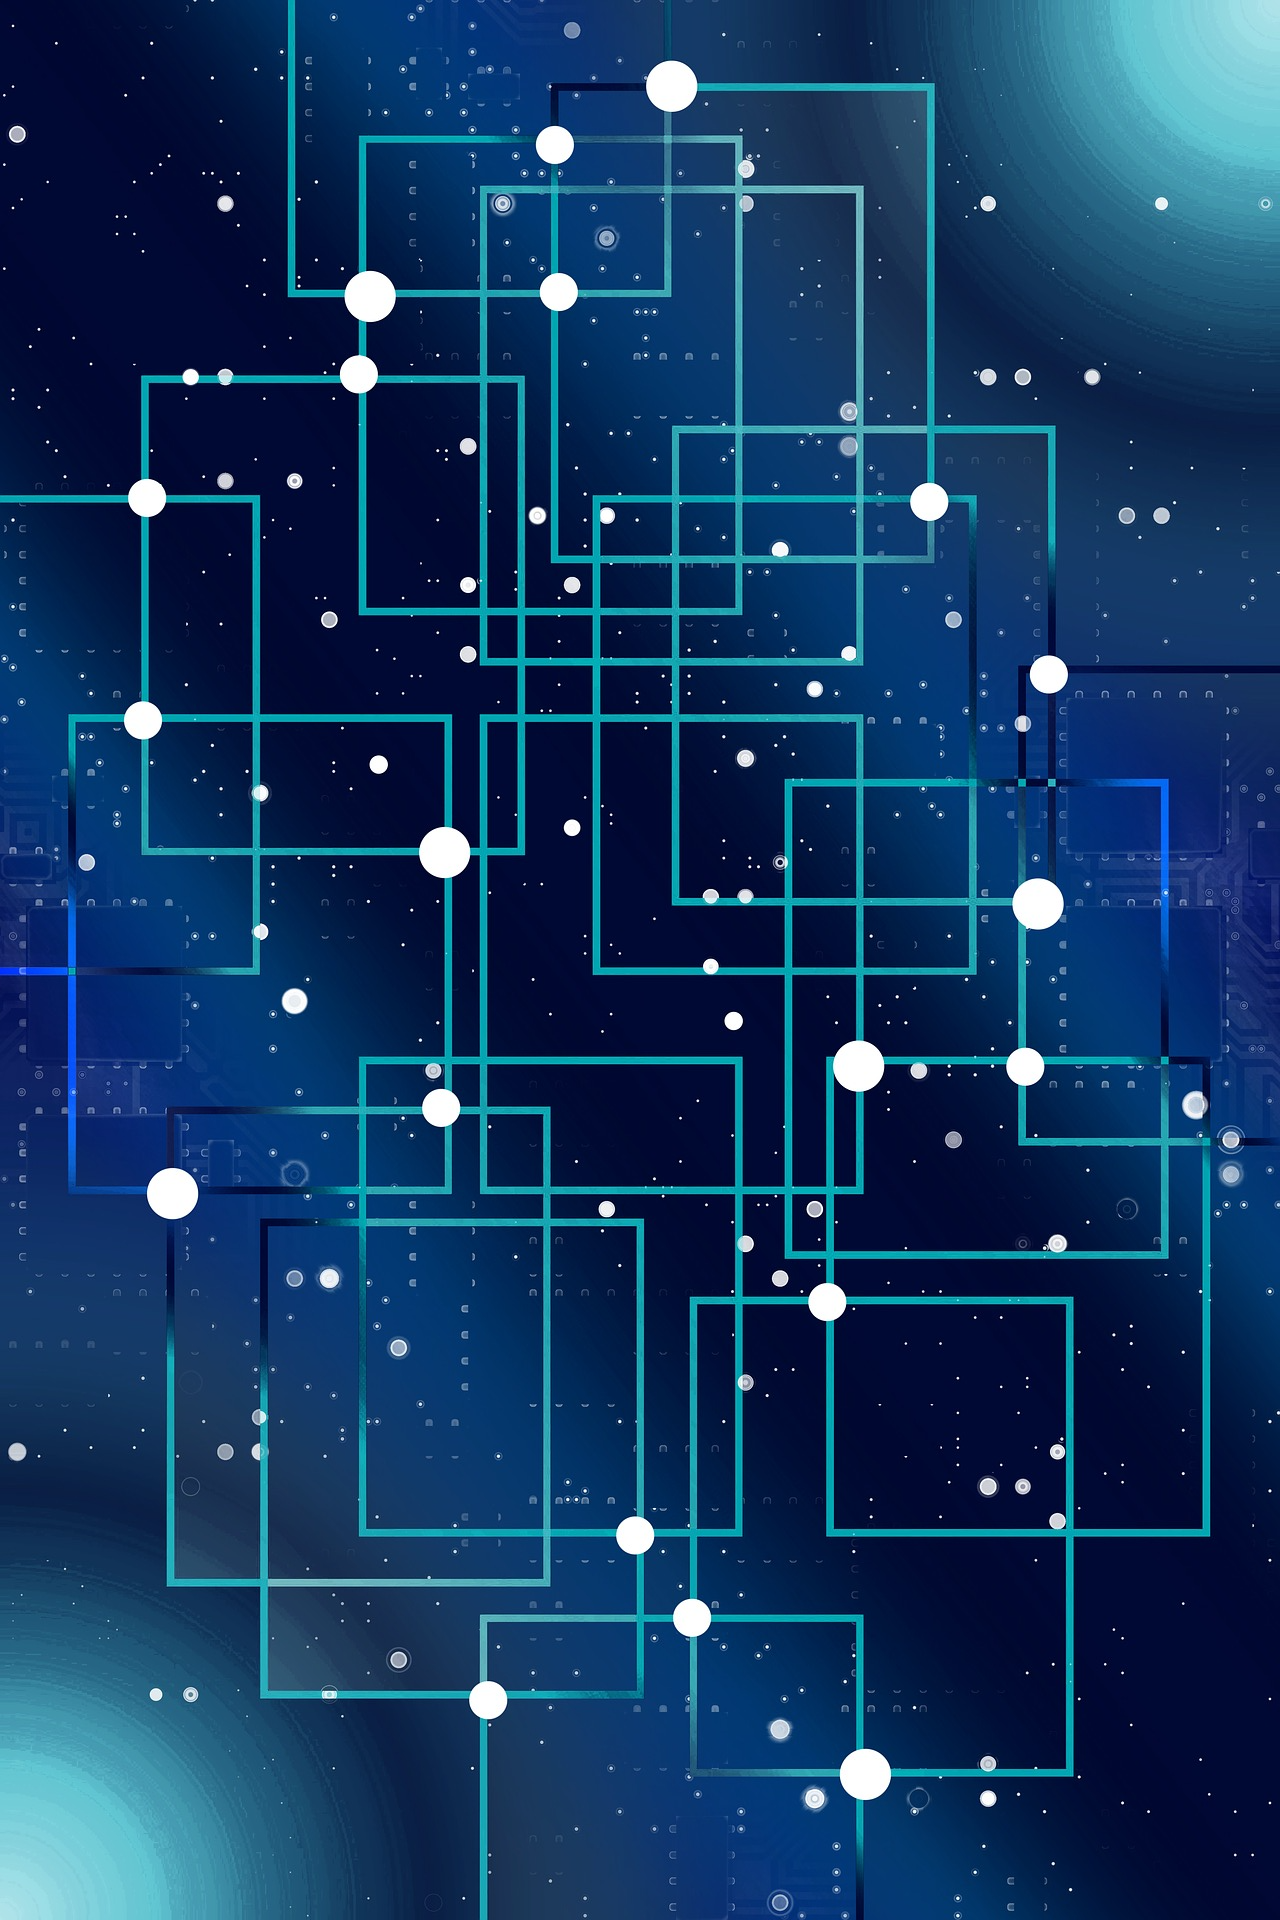
\includegraphics[width=\paperwidth]{background.png}};
\draw (current page.center) node [fill=blue!2!white,fill
opacity=0.9,text opacity=1,inner
sep=1cm]{\Huge\centering\bfseries\sffamily\parbox[c][][t]{\paperwidth}{\centering
    \TITLE \\[15pt] % Book title
{\Large \SUBTITLE}\\[20pt] % Subtitle
{\huge \AUTHOR \\ \Large \EMAIL }}}; % Author name
\end{tikzpicture}
\vfill
\endgroup

%----------------------------------------------------------------------------------------
%	COPYRIGHT PAGE
%----------------------------------------------------------------------------------------

\newpage
~\vfill
\thispagestyle{empty}

\noindent Copyright \copyright\ 2017 \AUTHOR \\

\noindent \EMAIL \\ % Copyright notice

% \noindent \textsc{Indiana University}\\ % Publisher

\noindent \textsc{https://github.com/cloudmesh/classes}\\ % URL

\begin{comment}
\noindent Licensed under the Creative Commons
Attribution-NonCommercial 3.0 Unported License (the ``License''). You
may not use this file except in compliance with the License. You may
obtain a copy of the License at
\url{http://creativecommons.org/licenses/by-nc/3.0}. Unless required
by applicable law or agreed to in writing, software distributed under
the License is distributed on an \textsc{``as is'' basis, without
  warranties or conditions of any kind}, either express or
implied. See the License for the specific language governing
permissions and limitations under the License.\\ % License information

\end{comment}

\noindent \textit{First printing, October 2017} % Printing/edition date

%----------------------------------------------------------------------------------------
%	TABLE OF CONTENTS
%----------------------------------------------------------------------------------------

%\usechapterimagefalse % If you don't want to include a chapter image, use this to toggle images off - it can be enabled later with \usechapterimagetrue

\chapterimage{TOC.png} % Table of contents heading image

\pagestyle{empty} % No headers

\tableofcontents % Print the table of contents itself

\cleardoublepage % Forces the first chapter to start on an odd page so it's on the right

\pagestyle{fancy} % Print headers again



\newcommand{\FILENAME}{\begin{fileremark}\currfiledir
    \currfilename\end{fileremark}}
\newcommand{\CHANGE}{\begin{changeremark}THIS WILL CHANGE
    \currfilename\end{changeremark}}
\newcommand{\TODO}[1]{\todo[inline]{#1}}
\newcommand{\DONE}[1]{DONE: \todo[inline,color=green!30]{#1}}

\newcommand{\FIGURE}[5]{
\begin{figure}[#1] 
  \centering 
    \includegraphics[width=#2\columnwidth]{#3} 
  \caption{#4}\label{#5} 
\end{figure} 
}

\newcommand{\URL}[1]{ \begin{footnotesize} \begin{itemize} \item \url{#1} \end{itemize} \end{footnotesize}}
\newcommand{\HREF}[2]{ \begin{itemize} \item \href{#1}{#2} \end{itemize} }

\newcommand{\video}[4]{%
{\em \hfill \href{#4}{#3 (#2)~
\includegraphics[width=\baselineskip]{images/video.png} }}    \index{Video!#1!#3 (#2)}
}

\newcommand{\slides}[4]{%
  {\em  \hfill \href{#4}{#3 (#2)~
\includegraphics[width=\baselineskip]{images/slide.png}}} \index{Slides!#1!#3 (#2)}
}

\DefineVerbatimEnvironment{verbatim}{Verbatim}{fontsize=\footnotesize,xleftmargin=.5in}


\definecolor{codegreen}{rgb}{0,0.6,0}
\definecolor{codegray}{rgb}{0.5,0.5,0.5}
\definecolor{codepurple}{rgb}{0.58,0,0.82}
\definecolor{backcolour}{rgb}{0.97, 0.97, 0.97}
 
\lstdefinestyle{code}{
    backgroundcolor=\color{backcolour},   
    commentstyle=\color{codegreen},
    keywordstyle=\color{magenta},
    numberstyle=\tiny\color{codegray},
    stringstyle=\color{codepurple},
    basicstyle=\footnotesize,
    breakatwhitespace=false,         
    breaklines=true,                 
    captionpos=b,                    
    keepspaces=true,                 
    numbers=left,                    
    numbersep=5pt,                  
    showspaces=false,                
    showstringspaces=false,
    showtabs=false,                  
    tabsize=2
}
 
\lstset{style=code}

\newcommand{\WHERE}[2]{$\square$~ \ref{#1}. \nameref{#1} \hfill ~ #2 ~ \pageref{#1}\\}

\newenvironment{NOTE2}[1]
    {\begin{tcolorbox}[colback=blue!5!white,colframe=blue!75!black,%
                       fonttitle=\bfseries,size=small,%
                       lefthand width=2cm,sidebyside,%
                       sidebyside gap=6mm,%
                       lower separated=false,title=#1]%
    {\begin{tikzpicture}[overlay]
\node[draw=ocre!60,line
width=1pt,circle,fill=ocre!25,font=\sffamily\bfseries,inner
sep=2pt,outer sep=0pt] at (25pt,0pt){\textcolor{ocre}{\LARGE Note}};\end{tikzpicture}}
    \tcblower}
    {\end{tcolorbox}}

\newenvironment{COLORNOTE}[2]
    {\begin{tcolorbox}[%
        coltitle=#2!70!black,
        colback=#2!3!white,colframe=#2!20!white,%
        fonttitle=\bfseries,size=small,%
        title=#1]}
    {\end{tcolorbox}}

\newenvironment{NOTE}
    {\begin{COLORNOTE}{Note}{blue}}
    {\end{COLORNOTE}}

\newenvironment{WARNING}
    {\begin{COLORNOTE}{Warning}{red}}
    {\end{COLORNOTE}}

\newenvironment{IU}
    {\begin{COLORNOTE}{Indiana University}{red}}
    {\end{COLORNOTE}}


\newcommand{\TODAY}{
\begin{itemize}
\item \today~\currenttime 
\end{itemize} 
}






\graphicspath{{./}{images/}{notebooks/opencv/}{notebooks/}}

\chapterimage{water.png} % Chapter heading image

%
%	END CONFIGURATION
%--------------------------------------------------------------------------------------



%--------------------------------------------------------------------------------------
%	EXAMPE FOR INCLUDING FIGURES

%\FIGURE{htb} 
%    {1.0}
%    {images/kubernetes.jpeg}
%    {The Architecture of the Framework}
%    {F:tas-arch} 

%
%	END EXAMPLES
%--------------------------------------------------------------------------------------





%----------------------------------------------------------------------------------------
%	INTRODUCTION
%----------------------------------------------------------------------------------------

%----------------------------------------------------------------------------------------
%	PART
%----------------------------------------------------------------------------------------

\part{Preface}



%----------------------------------------------------------------------------------------
%	CHAPTER
%----------------------------------------------------------------------------------------

\chapterimage{water.png} % Chapter heading image

\chapter{Introduction}

\FILENAME

\section{Authors}

\FILENAME

\begin{description}

\item[Gregor von Laszewski] Gregor von Laszewski is an Assistant
  Director DSC in the School of Informatics and Computing and
  Engeneering at Indiana University. He holds also a position as
  Adjunct Professor in the Intelligent Systems Engineering
  Department. Previously he held Adjunct Professor positions at the
  Computer Science Department at Indiana University and University of
  North Texas. He received a Ph.D. from Syracuse University in
  computer science.

  He served as the architect of the the FutureGrid project. He held a
  position at Argonne National Laboratory where he was last a
  scientist and a fellow of the Computationand part of the initial
  team working on Grid computing.

  At IU He served as the architect of the the FutureGrid project. His
  current interest and projects include cloud computing, big data, and
  scientific impact metrics, and edge computing.  He initiated the
  Cloudmesh project which is a toolkit to enable cloud computing
  across various Cloud and Container IaaS such as OpenStack, AWS,
  Azure, docker, docker swarm, and kubernetes.


\item[Geoffrey C. Fox] Fox received a Ph.D. in Theoretical Physics
  from Cambridge University and is now distinguished professor of
  Informatics and Computing, and Physics at Indiana University where
  he is director of the Digital Science Center, Chair of Department of
  Intelligent Systems Engineering and Director of the Data Science
  program at the School of Informatics, Computing, and Engineering.

  He currently works in applying computer science from infrastructure
  to analytics in Biology, Pathology, Sensor Clouds, Earthquake and
  Ice-sheet Science, Image processing, Deep Learning, Manufacturing,
  Network Science and Particle Physics. The infrastructure work is
  built around Software Defined Systems on Clouds and Clusters. The
  analytics focuses on scalable parallelism.

\item [Dr. Judy Qiu] is an Associate Professor in the School of
  Informatics and Computing at Indiana University. Her research
  interests focus on data-intensive computing at the intersection of
  cloud and multicore technologies, with an emphasis on life science
  applications using MapReduce as well as traditional parallel and
  distributed computing approaches. Her contributions are focused on
  Hadoop and Introdcution into Cloud Computing. 

\end{description}

\section{Acknowledgements}

Part \ref{P:chameleon} focussing on Chameleon Cloud was contributed by
Kate Kaheay the lead of the Chameleon Cloud project sponsored by NSF
grant 1743358, Collaborative Research: Chameleon: A Large-Scale,
Reconfigurable Experimental Environment for Cloud Research. Some
content has been modified and added by Gregor von Laszewski to target
specifically classes and education material targeted for Indiana
University.

\FILENAME

\section{About}\label{about}

This document is managed on \verb|github.com| at 

\URL{https://github.com/cloudmesh/book/}

The current release version is held in the master branch.
Development versions will be held under a number of branches:

\begin{description}
\item[e516] Branch with contributions from students of the e616
  class. Merges to and from the {\em latex} branch will be conducted
  on a daily bases by TA's.
\item[e616] Branch with contributions from students of the e616
  class. Merges to and from the {\em latex} branch will be conducted
  on a daily bases by TA's.
\item[latex] Branch managed by Gregor and the TA's
\item[master] Branch that contains the current released version. This
  version is updated once a week from the branch {\em latex}.
\end{description}

Contributions are to be conducted as pull requests. It is important to
keep the pull requests small and on a section or even paragraph
base. This helps avoiding conflicts at time of checkin and is a common
practice in large communities. It is not a good practice to work for
weeks on improvements and than issue the pull request. For sure things
will have changed and it will take you a long time to catch up.

The document is based on selected material published at the following
Web page

\URL{https://cloudmesh.github.io/classes/}


It is part of a classes taught at Indiana University. The class
communication takes place in piazza and you need to enroll in it via
CANVAS where you will find a panel for it.

The PDF version will be made in future available at 

\URL{https://github.com/laszewski/laszewski.github.io/raw/master/papers/vonLaszewski-bigdata.pdf}

This PDF document will be updated based on feedback from the students
and once we have now material available. 

\section{Citation}

The bibtex entry for this document is

\begin{verbatim}
@TechReport{las17handbook,
  author =       {Gregor von Laszewski and Geoffrey C. Fox and Judy Qui},
  title =        {Handbook of Clouds and Big Data -- Theory and Practice},
  institution =  {Indiana University},
  year =         {2018},
  OPTtype =      {Draft},
  address =      {Smith Research Center, Bloomington, IN 47408},
  month =        jan,
  url={https://github.com/laszewski/laszewski.github.io/raw/master/papers/vonLaszewski-bigdata.pdf},
}
\end{verbatim}

\section{Contributing}
\index{Contributing}

\subsection{Pull requests}

It is easy to contribute to this document and we invite everyone to
improve the material. To do so you need to fork the repository from 

\URL{https://github.com/cloudmesh/book/}

and clone it. Then you can modify information in the different files
or add new sections. It is important that you make changes based on
sections and than for them create a new pull request. This simplifies
the review process. We will typically want only one file to be
changed. Aslo before you issue your pull request make sure that no one
else has already made changes. In that case we ask you to integrate
them into your document.


\section{Results}\label{S:results}

In this section we list documents about BigData technologies and
Projects that have been delivered by students of past classes. As we
can not post any grades it is importan that you yourself identify good
examples from the published list. It is important not to make the
mistake to work towards minimal fulfillment of the class requirements,
but instead work towards achieving your best. All documents produced
by this class will be made available on github.com and through this
document. This helps other students to learn from your experience and
to counteract plagiarism. 

\begin{NOTE}
  Examples provided here may not necessarily meet the requirements for
  your current class as the content and requirements have changed
  since the other classes were thought. This includes format of the
  paper, paper length, as well as the topic for projects.
\end{NOTE}

\subsection{Introduction to Big Data Applications and Analytics}

This class was known under the name I523.

% this document needs to be deleted as it is temporary
% \URL{https://github.com/laszewski/laszewski.github.io/raw/master/papers/vonLaszewski-i523.pdf}

Application and Technologies (Vol.1):
\URL{https://github.com/laszewski/laszewski.github.io/raw/master/papers/vonLaszewski-i523-v1.pdf}

Application and Technologies (Vol. 2):
\URL{https://github.com/laszewski/laszewski.github.io/raw/master/papers/vonLaszewski-i523-v2.pdf}

Project: First 500 pages:
\URL{https://github.com/laszewski/laszewski.github.io/raw/master/papers/vonLaszewski-i523-v3-1.pdf}

Project: Second part, starting past page number501:
\URL{https://github.com/laszewski/laszewski.github.io/raw/master/papers/vonLaszewski-i523-v3-2.pdf}

\subsection{Big Data Applications and Open Source Software}

This class was known under the name I524

Big Data Software Vol 1.:
\URL{https://github.com/cloudmesh/sp17-i524/blob/master/paper1/proceedings.pdf}

Big Data Software Vol 2.:
\URL{https://github.com/cloudmesh/sp17-i524/blob/master/paper2/proceedings.pdf}

Big Data Projects:
\URL{https://github.com/cloudmesh/sp17-i524/blob/master/project/projects.pdf}


\subsection{Contributors}

We like to acknowledge the following contributors that helped on this
document. Please notify us with your name and a brief commend on what
you contributed:

Descriptions provided in Section \ref{s:} were contributed by the
following people that are either listed by full name or their
github.com id:

\begin{quotation}{\em
Abhijit Thakre, Abhishek Gupta, Abhishek Naik, Ajit Balaga, Anurag
Kumar Jain, Avadhoot Agasti, Badi' Abdul-Wahid, Cmbays, DIKSHA,
Dimitar Nikolov, Govind, Govind Mishra, Grace Li, Gregor von
Laszewski, Harshit Krishnakumar, Hyungro Lee, Jerome Mitchell, Jimmy
Ardiansyah, Jon, Jon Montgomery, Jordan Simmons, Juliette Zerick,
Karthik, Kumar Satyam, Mark McCombe, Matthew Lawson, Methkupalli
Vasanth, Miao Jiang, Miao Zhang, Milind Suryawanshi,
MilindSuryawanshi, Nandita Sathe, Naveen, Niteesh01, Piyush Rai,
Piyush Shinde, Prashanth, Pratik Jain, Rahul Raghatate, Rahul Singh,
Ribka Rufael, Ronak Parekh, Saber Sheybani, Sabyasachi Roy Choudhury,
Sagar Vora, Sahiti Korrapati, Scott McClary, Sean Shiverick,
SilviaKarim14, Sivaprasad Sushmita, Snehal Chemburkar, Sowmya Ravi,
Srikanth Ramanam, Sunanda Unni, SushmitaSivaprasad, Tony Liu, Vasanth
Methkupalli, Veera Marni, Vibhatha Abeykoon, Vibhatha Lakmal Abeykoon,
Vishwanath Kodre, William H Knapp III, acastrob, ak.15, alyez,
anveling, argetlam115, athakre, bhavesh37, cacoulte, cglmoocs,
elenadesigner, eunosm3, harkrish1, jemitchell, justbbusy, jzerick,
kartanba, karthick, karthick venkatesan, karthik-anba, kpvenkat,
ksrivatsav, lmundia, miaozhan, michaelsmith1983, mmccombe, nsathe,
piyurai, pratik11jain, ronak1182, sabyasachi087,
shah0112, sriramsitharaman, suunni, tifabi, tonythomascn, vasanth,
vibhatha, vkodre, vlabeyko, xl41, yatinsharma7
}\end{quotation}


\section{Conventions}
\index{Convention}

\subsection{Videos}

Videos to the class are referred to with embedded links into the PDF
document as follows: 

\video{About}{25:36}{Test Video}{https://www.youtube.com/watch?v=yC3PNkb_9mI}

An index will also be available in the index page
that lists on which page the video has been added.

\subsection{Slides}

Sides
\slides{About}{10}{Test slides}{PUT URL HERE}

\subsection{Images}

The video icon was copied from \url{http://www.freeiconspng.com/img/8039}.

\subsection{URLs}

The online version of this document contains a significant number of
links. The links are either embedded or are directly visible. The
color of the links is blue.

\begin{description}
\item[Direct URL:] This is an example for a
  \url{https://github.com/cloudmesh/book/}
\item[Embedded URL:] This is an example for an embedded URL that
  points to the \href{https://github.com/cloudmesh/book/}{source on github}

\end{description}

\section{Exercise}

\begin{description}
\item[Exercise.1:] Inspect the PDF documents produced by previous
classes. Note the differences between technology and application
reviews and projects. 
\end{description}
\section{About the Document}\label{about-the-document}

The material in this document is covering material that is used in the
following classes at Indiana University.

Undergraduate couses:

\begin{itemize}
\tightlist
\item E222 Intelligent systems II
\end{itemize}

Graduate courses:

\begin{itemize}
\tightlist
\item E516 Introduction to Cloud Computing
\item E616 Advanced Cloud Computing
\item E534 Big Data Applications
\end{itemize}

Material from earlier classes known under the numbers I523 and I524 and
Introduction to cloud computing have havily influenced this material.
The collection of this material is updated continiously and new versions
will be made available throughout the semester.

We encourage students of the classes to contribute to this material,
provide corrections, and additions.

\subsection{New chapters under
development}\label{new-chapters-under-development}

The following new chapters are under cdevelopment:

\begin{itemize}
\item Building a Cloud Cluster
\item Introduction to Containers
\item Docker
\item Docker Swarm
\item Introduction to Kubernetes
\item Kubernetes
\item Minikube
\item Pi Kubernetes cluster
\end{itemize}

More will be added here.

\subsection{Preliminary Outline}\label{preliminary-outline}

\begin{itemize}
\item About the Document
\item Scientific Writing

  \begin{itemize}
  \tightlist
  \item   Plagiarizm
  \item   LaTeX
  \item   BibTeX
  \end{itemize}
\item Essential Technologies

  \begin{itemize}
  \item   Linux
  \item   SSH
  \item   Programming Languages

    \begin{itemize}
    \tightlist
    \item     Python
    \item     Go
    \item     Java
    \end{itemize}
  \item   Code Management
  \item   Git
  \item   Github
  \item   Gitlab
  \end{itemize}
\item Cloud Computing

  \begin{itemize}
  \item   IaaS

    \begin{itemize}
    \item     OpenStack
    \item     Chameleon Cloud
    \end{itemize}
  \item   PaaS
  \item   SaaS
  \item   MapReduce

    \begin{itemize}
    \tightlist
    \item     Word Count
    \item     K-Means
    \end{itemize}
  \item   Containers

    \begin{itemize}
    \tightlist
    \item     LXD
    \item     Docker
    \item     Docker Swarm
    \item     Kubernetes
    \item     PI Cluster
    \item     Echo
    \end{itemize}
  \end{itemize}
\item Big Data

  \begin{itemize}
  \tightlist
  \item   integrate i523 and i524
  \end{itemize}
\item Edge Computing
\item Internet of Things
\end{itemize}





\part{Syllabus}


%%%%%%%%%%%%%%%%%%%%%%%%%%%%%%%%%%%%%%%%%%%%%%%%%%%%%%%%%%%%%%%%%%%%%%
\chapter{E516: Introduction to Cloud Computing}
%%%%%%%%%%%%%%%%%%%%%%%%%%%%%%%%%%%%%%%%%%%%%%%%%%%%%%%%%%%%%%%%%%%%%%

We present the syllabus for the introduction to Cloud Computing course
taught at Indiana University that uses in part the material presented
in this document. The information includes the section or chapter
number, the name of the chapter or section, and the timeframe when it
is recommended to work through the material and the page number where
to find the material in this document. Please note that we will update
the document throughout the semester thus, pagenumbers will change. 

\section{Course Description}

This course describes the emerging cloud and big data technologies
within the world of distributed intelligent systems where each system
component has internal, and external sources of intelligence that are
subject to collective control. Examples are given from a wide variety
of applications. A project will allow students to dive into practical
issues after they have obtained a theoretical background.

\section{Course pre-requisites}

Python will be used as a Programming Languages. In some cases Java may
also be useful however it's use in class will be marginal. The class
will be using Linux commandline tools. Prior knowledge of Linux is of
advantage but not required.  Studnets are expected to have access to a
computer on which they can execute Linux easily. As the OS
requirements have recently increased we recommend a computer with 8GB
main memory and the ability to run virtualbox and/or containers. If it
turns out your machine is not capable enough we attempt to provide
access to IU linux machines.

\section{Registration Information}

\begin{verbatim}
ENGR-E 516  ENGINEERING CLOUD COMPUTING (3 CR)
       33699 RSTR     11:15A-12:30P   F      I2 150    Von Laszewski G
          Above class taught online
          Above class open to graduates only
          Discussion (DIS)


ENGR-E 516  ENGINEERING CLOUD COMPUTING (3 CR)
       33909 RSTR     ARR             ARR    WB WEB    Von Laszewski G
          This is a 100% online class taught by IU Bloomington. No
          on-campus class meetings are required. A distance education
          fee may apply; check your campus bursar website for more
          information
          Above class open to graduates only
\end{verbatim}


\section{Teaching and learning methods}


\begin{itemize}
\item Lectures
\item Assignments including specific lab activities
\item Final project 
\end{itemize}

\section{Covered Topics}

The class will cover a number of topics as part of tracks that are
executed in parallel throughout the class. Although we assume that at
a graduate course level the communication track has already been
covered elsewhere, we made sure we also include it here in case you dod
not yet have such experiences.

\begin{itemize}

\item {\bf Week 1: Course Overview:} Overview and status of cloud
\item {\bf Week 2-3: Introduction:} Overview and status of cloud
  computing. This includes the creation of REST services for Big Data
\item {\bf Week 4-5: Cloud Computing:} Basics of Cloud Computing 
\item {\bf Week 6-7: Virtual Machines:} Introduction to OpenStack
\item {\bf Week 8-9: Cloud 3.0:} Microservices, Events, Functions  
\item {\bf Week 10-13: Hadoop:} Introduction to Hadoop
\item {\bf Week 13-15: Project:} Delivery of a reproducible
  substantial student project
 
\end{itemize}

\section{Student learning outcomes}

When students complete this course, they should be able to:

\begin{itemize}
\item Have an elementary understanding of issues involved in designing
  and Software Defined Systems.
\item Understand the concepts of Cloud Computing
\item Gain hands-on laboratory experience with several examples.
\item Apply knowledge of mathematics, science, and engineering
\item	Have advanced skills in teamwork with peers.
\end{itemize}

\section{Grading}

\begin{tabular}{lr}
Grade Item	  & Percentage\\
\hline
Assignments	  & 40\% \\
Final Project	& 50\% \\
Participation	& 10\% \\
\hline
\end{tabular}




\section{Representative bibliography}

\begin{enumerate}
\item Cloud Computing for Science and Engineering By Ian Foster and
  Dennis
  B. Gannon\URL{https://mitpress.mit.edu/books/cloud-computing-science-and-engineering}
\item Ansible Tutorials
\item	\url{http://bigdataopensourceprojects.soic.indiana.edu/}
\item The backdrop for course is the ~350 software subsystems
  illustrated at \url{http://hpc-abds.org/kaleidoscope/}
\item	\url{http://cloudmesh.github.io/introduction_to_cloud_computing/}
\item	There are a huge number of web resources

\item (This document) {\bf Handbook of Clouds and Big Data}, Gregor von Laszewski,
  Geoffrey C. Fox, and Judy Qiu, Fall 2017,
  \url{https://tinyurl.com/vonLaszewski-handbook}

\item {\bf Use Cases in Big Data Software and
  Analytics Vol. 1}, Gregor von Laszewski, Fall 2017,
  \url{https://tinyurl.com/cloudmesh/vonLaszewski-i523-v1.pdf}

\item {\bf Use Cases in Big Data Software and
  Analytics Vol. 2}, Gregor von Laszewski, Fall 2017, \url{https://tinyurl.com/cloudmesh/vonLaszewski-i523-v2.pdf}

\item  {\bf Use Cases in Big Data Software and
  Analytics Vol. 3}, Gregor von Laszewski, Fall 2017, 
  \url{https://tinyurl.com/vonLaszewski-projects-v3}

\item (Draft) {\bf Big Data Software Vol 1.}, Gregor von Laszewski, Spring 2017,
\url{https://github.com/cloudmesh/sp17-i524/blob/master/paper1/proceedings.pdf}

\item (Draft) {\bf Big Data Software Vol 2.}, Gregor von Laszewski, Spring 2017,
\URL{https://github.com/cloudmesh/sp17-i524/blob/master/paper2/proceedings.pdf}

\item (Draft) {\bf Big Data Projects}, Gregor von Laszewski, Spring 2017,
\URL{https://github.com/cloudmesh/sp17-i524/blob/master/project/projects.pdf}

\end{enumerate}

\section{Lectures and Lecture Material}\label{S:lectures-516}

\begin{WARNING}
This section will change and be updated throughout the semester
\end{WARNING}


\begin{IU}

To start the class at IU, we require you to watch the following video:

% \slides{Overview}{45}{TBD}{https://drive.google.com/open?id=yyy}
\video{Class Management}{39:54}{Class Management -
  Overview}{https://youtu.be/azCXscVSZQc}

\video{Teaching Cloud and Big Data}{39:54}{Teaching Cloud and Big Data - Overview}{https://youtu.be/sJRMAbFz4hs}
\end{IU}

\subsection{Assignments}

All assignments are summarized in the Section \ref{s:616-assignments}

The current released assignments include:

\WHERE{\YES}{a:616-bio}{Due: Jan 22, 2018}
\WHERE{\YES}{E:616-bigdata-collab}{Due: Jan 29, 2018}
\WHERE{\YES}{E:616-new-tech}{Due: Jan 29, 2018}
\WHERE{\YES}{E:616-new-tech-abstract}{Due: Jan 29, 2018}


\subsection{Communication Track}

\WHERE{\YES}{S:lectures-516}{Week 1}
\WHERE{\YES}{C:doc}{Month 1}
\WHERE{\YES}{S:plagiarism}{Week 1}
\WHERE{\YES}{S:results}{Week 1}

\WHERE{\YES}{S:markdown}{Week 1}
\WHERE{\YES}{C:emacs}{Week 2}

\WHERE{\YES}{S:writing}{Week 3}
\WHERE{\YES}{C:latex}{Week 3}
\WHERE{\YES}{C:bibtex}{Week 4}

\begin{description}
\item[Evaluation Paper1:] Create a paper about a cloud technology with
  our give class template in the git repository. If a paper is
  plagiarized you will receive an ``F'' and it is reported based on
  University policies.
\end{description}


\subsection{Theory Track}

\begin{itemize}
\item IaaS - OpenStack
\item PaaS - Hadoop
\item SaaS - SaaS with REST
\end{itemize}

\begin{description}
\item[Evaluation Paper1:] Create a paper about a cloud technology with
  our give class template in the git repository. If a paper is
  plagiarized you will receive an ``F'' and it is reported based on
  University policies. The paper is in a directory called paper1. All
  images are in the directory paper1/images, the report is in
  report.tex, the content is in content.tex. It follows the template
  we provided. Submission of report.pdf is not allowed. We will create
  the report and check completness that way.
\end{description}

\subsection{Programming Track}

\subsubsection{Development Environment}

\WHERE{\YES}{S:virtual-box}{Week 2}
\WHERE{\YES}{C:linux}{Week 2}
\WHERE{\NO}{C:ssh}{Week 2}
\WHERE{\NO}{C:github}{Week 3}


\begin{description}
\item[Evaluation Experiment 1:] Create a virtual machine and take a
  photo with your laptop or computer and the virtual box running on
  the screen. Showcase the virtual box interface and in non full
  screen mode at the same time the operating system you run. We
v  recommend yo use Ubuntu.
\end{description}

\subsubsection{Python}

\WHERE{\YES}{C:python}{Week 3 - 4}
\WHERE{\YES}{C:python-install}{Week ?}
\WHERE{\YES}{C:python-language}{Week ?}
\WHERE{\YES}{C:python-lib}{Week ?}
\WHERE{\NO}{C:python-cmd5}{Week ?}

\subsubsection{Cloud}

\WHERE{\YES}{s:rest-intro}{Week 2}
\WHERE{\YES}{s:eve-intro}{Week 2}
\WHERE{\YES}{c:swagger-codegen}{Week 3}


\paragraph{Assignments}

Develop a Big Data related REST service with swagger.

Chose two of them so you can see the difference between the APIs:

\begin{itemize}
\item Build a Multi cloud interface to OpenStack
\item Build a Multi cloud interface to AWS
\item Build a Multi cloud interface to Azure
\item Build a Multi cloud interface to Docker/Kubernetes
\end{itemize}


\begin{description}
\item[Evaluation Experiment 1:] Create a program in python that
  identifies a termination criteria for the Secchi disk
  problem. E.g. at what image can we no longer see the disk?
  Describe your solution in md and submit to the git repository in a
  directory called {\em secchi}. The program is called secchi.py, the
  description is in README.md. It uses cmd5 for creating a command
  shell that can load the data and analyze it. 
\item[Evaluation Assignment 1:] Create two a REST service for Big Data
  with swagger and provide a python implementation from the exported
  python code to provide real functionality.
\item[Evaluation Assignment 2:] Develop cloudmesh extensions to access
  cloud services from 2 different providers.
\end{description}

\subsubsection{Chameleon Cloud and OpenStack}

\WHERE{\YES}{C:chameleon}{Week 4}
\WHERE{\YES}{C:cc-charge}{Week 4}
\WHERE{\YES}{C:cc-hardware}{Week 4}
\WHERE{\YES}{C:cc-start}{Week 4}
\WHERE{\YES}{C:cc-horizon}{Week 5}
\WHERE{\YES}{C:cc-guide}{Week 4}
\WHERE{\NO}{C:cc-heat}{Optional}
\WHERE{\NO}{C:cc-baremetal}{Optional}


%%%%%%%%%%%%%%%%%%%%%%%%%%%%%%%%%%%%%%%%%%%%%%%%%%%%%%%%%%%%%%%%%%%%%%
\chapter{E616/I524: Advanced Cloud Computing}
%%%%%%%%%%%%%%%%%%%%%%%%%%%%%%%%%%%%%%%%%%%%%%%%%%%%%%%%%%%%%%%%%%%%%%

This class is also known under the name {\em I524 Big Data
Applications and Open Source Software.}
 

We present the syllabus for the E616 course taught at Indiana
University that uses in part the material presented in this
document. The information includes the section or chapter number, the
name of the chapter or section, and the timeframe when it is
recommended to work through the material and the page number where to
find the material in this document. Please note that we will update
the document throughout the semester thus, page numbers will change.

\section{Course Description }

This course describes Cloud 3.0 in which DevOps, Microservices, and
Function as a Service is added to basic cloud computing. The
discussion is centered around the Apache Big Data Stack and a major
student project aimed at demonstrating integration of cloud
capabilities.

\section{Course pre-requisites}

Python will be used as a Programming Languages. It is expected that
you know a programming language. ENGR-E516 or an introduction to cloud
computing is recommended. Studnets are expected to have access to a
computer on which they can execute Linux easily. As the OS
requirements have recently increased we recommend a computer with 8GB
main memory and the ability to run virtualbox and/or containers. If it
turns out your machine is not capable enough we attempt to provide
access to IU linux machines.

\section{Course Registration}

I524 and E616 are identical. In this courses we will be focussing on
Advanced Cloud COmputing and Big Data Applications and Analytics. 

Intelligent Systems Engeneering Residential:

\begin{verbatim}
	ENGR-E 616  ADVANCED CLOUD COMPUTING (3 CR)
              ***** RSTR     ARR             ARR    ARR       Von Laszewski G
                 Above class taught online
                 Above class open to graduates only
                 Discussion (DIS)
              33697 RSTR     09:30A-10:45A   F      I2 150    Von Laszewski G
\end{verbatim}

Info Residential:

\begin{verbatim}
INFO-I 524  BIG DATA SOFTWARE AND PROJECTS (3 CR) 
              ***** RSTR     ARR             ARR    ARR       Von Laszewski G          
                 Above class open to graduates only
                 Above class taught online
                 Discussion (DIS)
              13053 RSTR     09:30A-10:45A   F      I2 150    Von Laszewski G  
\end{verbatim}

Info Online:

\begin{verbatim}        
        INFO-I 524  BIG DATA SOFTWARE AND PROJECTS (3 CR)
              13054 RSTR     ARR             ARR    ARR       Von Laszewski G          
                 Above class open to graduates only
                 This is a 100% online class taught by IU Bloomington. No
                 on-campus class meetings are required. A distance education
                 fee may apply; check your campus bursar website for more
                 information
\end{verbatim}


\section{Teaching and learning methods}

\begin{itemize}
\item	Lectures
\item	Assignments including specific lab activities
\item	Final project
\item Class will use software mainly written in Python
  and Linux Shell.
\end{itemize}


\section{Covered Topics}

The class will cover a number of topics as part of tracks that are
executed in parallel throughout the class. Although we assume that at
a graduate course level the communication track has already been
covered elsewhere, we made sure we also include it here in case you did
not yet have such experiences.

Please note that we may change the order of the lectures. This is our
current plan

\begin{itemize}

\item {\bf Week 1-2: Introduction} Overview and status of cloud
  computing
\item {\bf Week 2: Cloud REST Services} Introduction to REST services
  to develop cloud services.
\item {\bf Weeb 3: Big Data Reference Architecture:} Using REST
  services to implement Big Data Services.
\item {\bf Week 4: Cloud and Big Data Applications:} Introduction to
  the Apache Big Data Stack. Selective presentation of the members of
  the Big Data Application set
\item {\bf 5: New Cloud Big Data Application Technologies:} Students will
  explore the Apache Web page and report on them. Continuation of
  earlier assigned homwework, including paper.
\item {\bf Week 6: DevOps:} Introduction to DevOps with Dokerfile and
  ansible
\item {\bf Week 7-14: Building a Kubernetes Cluster:} Residential
  students will be building a kubernetes cluster with 5
  servers. Online students could do that also, but need to simulate
  the cluster instead of using real hardware as it requires physical
  access to the hardware.

\item {\bf Week 7: Virtual Machines:} Introduction to OpenStack
\item {\bf Week 8-9: Containers:} Introduction to Container technology
\item {\bf Week 10: Advanced Containers:} Building clusters with containers.
\item {\bf Week 11: Cloud 3.0:} Microservices, Events, Functions  
\item {\bf Week 12-14: Project:} Delivery of a reproducible substantial
  student project (you are allowed to substantially enhance a project
  that you started from other cloud classes you took with us. Please ask.)
\end{itemize}

\section{Student learning outcomes}

When students complete this course, they should be able to:

\begin{itemize}
\item Have an advanced understanding of issues involved in designing
  and applying modern cloud technologies using the latest
  developments.
\item	Gain hands-on laboratory experience.
\item	Understand the Apache Big Data Software Stack.
\item	Apply knowledge of mathematics, science, and engineering.
\item Understand research challenges and important application areas
  of clouds
\item	Have advanced skills in teamwork with peers.
\item Be able to use DevOps technologies.
\end{itemize}

\section{Grading}


\begin{tabular}{lr}
Grade Item	  & Percentage\\
\hline
Assignments	  & 40\% \\
Final Project	& 50\% \\
Participation	& 10\% \\
\hline
\end{tabular}



\section{Representative bibliography}

\begin{enumerate}
\item Cloud Computing for Science and Engineering By Ian Foster and
  Dennis
  B. Gannon\URL{https://mitpress.mit.edu/books/cloud-computing-science-and-engineering}
\item	Machine to machine protocols \url{https://en.wikipedia.org/wiki/MQTT}
\item	Cloud software systems \url{http://hpc-abds.org/kaleidoscope/}
\item	Software Defined Networks \url{https://en.wikipedia.org/wiki/Software-defined_networking}
\item	There are a huge number of other web resources

\item (This document) {\bf Handbook of Clouds and Big Data}, Gregor von Laszewski,
  Geoffrey C. Fox, and Judy Qiu, Fall 2017,
  \url{https://tinyurl.com/vonLaszewski-handbook}

\item {\bf Use Cases in Big Data Software and
  Analytics Vol. 1}, Gregor von Laszewski, Fall 2017,
  \url{https://tinyurl.com/cloudmesh/vonLaszewski-i523-v1.pdf}

\item {\bf Use Cases in Big Data Software and
  Analytics Vol. 2}, Gregor von Laszewski, Fall 2017, \url{https://tinyurl.com/cloudmesh/vonLaszewski-i523-v2.pdf}

\item  {\bf Use Cases in Big Data Software and
  Analytics Vol. 3}, Gregor von Laszewski, Fall 2017,   
  \url{https://tinyurl.com/vonLaszewski-projects-v3}

\item (Draft) {\bf Big Data Software Vol 1.}, Gregor von Laszewski, Spring 2017,
\url{https://github.com/cloudmesh/sp17-i524/blob/master/paper1/proceedings.pdf}

\item (Draft) {\bf Big Data Software Vol 2.}, Gregor von Laszewski, Spring 2017,
\URL{https://github.com/cloudmesh/sp17-i524/blob/master/paper2/proceedings.pdf}

\item (Draft) {\bf Big Data Projects}, Gregor von Laszewski, Spring 2017,
\URL{https://github.com/cloudmesh/sp17-i524/blob/master/project/projects.pdf}

\end{enumerate}


\section{Lectures and Lecture Material}\label{S:lectures-616}

\begin{WARNING}
This section will change and be <updated throughout the semester
\end{WARNING}

\begin{IU}

To start the class at IU, we require you to watch the following video:

% \slides{Overview}{45}{TBD}{https://drive.google.com/open?id=yyy}
\video{Class Management}{39:54}{Class Management -
  Overview}{https://youtu.be/azCXscVSZQc}

\video{Teaching Cloud and Big Data}{39:54}{Teaching Cloud and Big Data - Overview}{https://youtu.be/sJRMAbFz4hs}

\end{IU}

\subsection{Assignments}

All assignments are summarized in the Section \ref{s:616-assignments}

The current released assignments include:

\WHERE{\YES}{a:616-bio}{Exercise \ref{E:616-bio-piazza},
  \ref{E:616-bio-googledocs}, \ref{E:616-iu-google} Due: Jan
  22, 2018}
\WHERE{\YES}{E:616-bigdata-collab}{Due: Jan 29, 2018}
\WHERE{\YES}{E:616-new-tech}{Due: Jan 29, 2018}
\WHERE{\YES}{E:616-new-tech-abstract}{Due: Jan 29, 2018}

\subsection{Communication Track}

\WHERE{\YES}{S:lectures-616}{Week 1}
\WHERE{\YES}{C:doc}{Month 1}
\WHERE{\YES}{S:plagiarism}{Week 1}
\WHERE{\YES}{S:results}{Week 1}

\WHERE{\YES}{S:markdown}{Week 1}
\WHERE{\YES}{C:emacs}{Week 2}

\WHERE{\YES}{S:writing}{Week 3}
\WHERE{\YES}{C:latex}{Week 3}
\WHERE{\YES}{C:bibtex}{Week 4}

\begin{description}
\item[Evaluation Paper1:] Create a paper about a cloud technology with
  our give class template in the git repository. If a paper is
  plagiarised you will receive an ``F'' and it is reported based on
  University policies.
\end{description}


\subsection{Theory Track}

\WHERE{\NO}{S:o-workflow}{Week 1}
\WHERE{\NO}{S:o-application}{Week 2}
\WHERE{\NO}{S:o-programming}{Week 3}
\WHERE{\NO}{S:o-streams}{Week 4}
\WHERE{\NO}{S:o-prg-model}{Week 5}
\WHERE{\NO}{S:o-process-communication}{Week 5}
\WHERE{\NO}{S:o-db-memory}{Week 6}
\WHERE{\NO}{S:o-db-object}{Week 6}
\WHERE{\NO}{S:o-Tools}{Week 7}
\WHERE{\NO}{S:o-sql}{Week 6}
\WHERE{\NO}{S:o-NoSQL}{Week 6}
\WHERE{\NO}{S:o-file-management}{Week 8}
\WHERE{\NO}{S:o-data-transport}{Week 8}
\WHERE{\NO}{S:o-cluster}{Week 9}
\WHERE{\NO}{S:o-file-systems}{Week 8}
\WHERE{\NO}{S:o-interoperability}{Week 3}
\WHERE{\NO}{S:o-DevOps}{Week 10}
\WHERE{\NO}{S:o-hypervisors}{Week 11}
\WHERE{\NO}{S:o-cross-cutting-functions}{Week 12}
\WHERE{\NO}{S:o-protocols}{Week 13}
\WHERE{\NO}{S:o-todo}{Week 4}


\begin{description}
\item[Evaluation Paper1:] Create a paper about a cloud technology with
  our give class template in the git repository. If a paper is
  plagiarized you will receive an ``F'' and it is reported based on
  University policies. The paper is in a directory called paper1. All
  images are in the directory paper1/images, the report is in
  report.tex, the content is in content.tex. It follows the template
  we provided. Submission of report.pdf is not allowed. We will create
  the report and check completness that way.
\end{description}

\subsection{Programming Track}

\subsubsection{Development Environment}

\WHERE{\YES}{S:virtual-box}{Week 2}
\WHERE{\YES}{C:linux}{Week 2}
\WHERE{\NO}{C:ssh}{Week 3}
\WHERE{\NO}{C:github}{Week 3}


\begin{description}
\item[Evaluation Experiment 1:] Create a virtual machine and take a
  photo with your laptop or computer and the virtual box running on
  the screen. Showcase the virtual box interface and in non full
  screen mode at the same time the operating system you run. We
  recommend yo use Ubuntu.
\end{description}

\subsubsection{Python}

\WHERE{\YES}{C:python}{Week 3 - 4}
\WHERE{\YES}{C:python-install}{Week ?}
\WHERE{\YES}{C:python-language}{Week ?}
\WHERE{\YES}{C:python-lib}{Week ?}
\WHERE{\NO}{C:python-cmd5}{Week ?}

\WHERE{\NO}{c:numpy}{}
\WHERE{\NO}{c:scipy}{} 
\WHERE{\NO}{c:opencv}{}
\WHERE{\NO}{c:secchi-disk}{}

\begin{description}
\item[Evaluation Experiment 1:] Create a program in python that
  identifies a termination criteria for the Secchi disk
  problem. E.g. at what image can we no longer see the disk?
  Describe your solution in md and submit to the git repository in a
  directory called {\em secchi}. The program is called secchi.py, the
  description is in README.md. It uses cmd5 for creating a command
  shell that can load the data and analyze it. 
\end{description}

\subsection{DevOps}

\begin{itemize}
\item ssh for DevOps
\item Ansible
\item Dokerfile
\end{itemize}

\subsection{Cloud}

\WHERE{\YES}{s:rest-intro}{Week 2}
\WHERE{\YES}{s:eve-intro}{Week 2}
\WHERE{\YES}{c:swagger-codegen}{Week 3}

\begin{itemize}
\item OpenAPI REST Service
\item OpenAPI Big Data Services
\item Deploy cloud services with Ansible
\end{itemize}

\subsubsection{Chameleon Cloud and OpenStack}

\WHERE{\YES}{C:chameleon}{Week 4}
\WHERE{\YES}{C:cc-charge}{Week 4}
\WHERE{\YES}{C:cc-hardware}{Week 4}
\WHERE{\YES}{C:cc-start}{Week 4}
\WHERE{\YES}{C:cc-horizon}{Week 5}
\WHERE{\YES}{C:cc-guide}{Week 4}
\WHERE{\NO}{C:cc-heat}{Optional}
\WHERE{\NO}{C:cc-baremetal}{Optional}


\section{Containers}

\begin{itemize}
\item Introduction to Docker - Docker File
\item Advanced Docker - Doker Swarm -  Kubernetes
\item Deploy cloud services with Doker/Kubernetes
\item Build a Raspberry Pi based Kubernetes cluster with 5 nodes
  (residential student can work on this in teams up to 5 students, we
  have 50 Raspberry Pi's)
\item Benchmark a 144 node Raspberry PI kubernetes cluster after
  deploying it (open class work)
\end{itemize}

%%%%%%%%%%%%%%%%%%%%%%%%%%%%%%%%%%%%%%%%%%%%%%%%%%%%%%%%%%%%%%%%%%%%%%
\chapter{E222: Intelligent Systems Engineering II}
%%%%%%%%%%%%%%%%%%%%%%%%%%%%%%%%%%%%%%%%%%%%%%%%%%%%%%%%%%%%%%%%%%%%%%

\section{Course Description}

In this undergraduate course students will be familiarized with
different specific applications and implementations of intelligent
systems and their use in desktop and cloud solutions.

\section{Course pre-requisites}

One programming language, Intelligent Systems Engineering I or equivalent

\section{Course Registration}


\begin{verbatim}
ENGR-E 222  INTELLIGENT SYSTEMS II (3 CR)
              ***** RSTR     02:30P-03:45P   TR     GY 436  Fox
                 Laboratory (LAB)
        E 222 : P - ENGR-E 221
              31434 RSTR     05:45P-06:35P   R      GY 447  Fox
                 Above class for  Intelligent Systems Engineering students

\end{verbatim}        


\section{Teaching and learning methods}


\begin{itemize}
\item Lectures
\item Assignments including specific lab activities
\item Final project 
\end{itemize}

\section{Covered Topics}

The topics covered in thie class include.

\begin{itemize}
\item Introduction to REST: Theory and Practice - develop a REST service
\item Introduction to Clouds: Theory and Practice - create via a
  program virtual machines and start on them the REST service
\item Introduction to Kubernetes: Theory and Practice - create a
  container that runs a REST service
\item Introduction to Advanced AI: Integrate your AI engine into a
  REST service and run on a cloud and in Kubernetes 
\item Introduction to Hadoop: Theory and Practice - Run Hadoop in a
  container; run hadoop on a futuresystems cluster
\item Edge Computing: Theory and Practice - Integrate Sensordata into
  Cloud Services via REST and MQTT
\end{itemize}


\section{Student learning outcomes}

When students complete this course, they should be able to:

\begin{itemize}
\item Have an elementary understanding of issues involved in Cloud
  Computing as part of the intelligent systems effort.
\item Gain hands-on laboratory experience with several examples.
\item Apply knowledge of mathematics, science, and engineering
\item Understand research challenges and important issues with
  Software Defined Systems.
\item	Have advanced skills in teamwork with peers.
\item Have theoretical and practical knowledge about REST, Clouds,
  Containers, and Edge Computing.
\end{itemize}


\section{Grading}

\begin{tabular}{lr}
  Grade Item	  & Percentage\\
  \hline
  Assignments	  & 60\%\\
  Final Project	& 30\%\\
  Participation	& 10\%\\
  \hline
\end{tabular}


\section{Representative bibliography}

\begin{enumerate}

\item Cloud Computing for Science and Engineering By Ian Foster and
  Dennis
  B. Gannon\URL{https://mitpress.mit.edu/books/cloud-computing-science-and-engineering}


\item (This document) {\bf Handbook of Clouds and Big Data}, Gregor von Laszewski,
  Geoffrey C. Fox, and Judy Qiu, Fall 2017,
  \url{https://tinyurl.com/vonLaszewski-handbook}

\item {\bf Use Cases in Big Data Software and
  Analytics Vol. 1}, Gregor von Laszewski, Fall 2017,
  \url{https://tinyurl.com/cloudmesh/vonLaszewski-i523-v1.pdf}

\item {\bf Use Cases in Big Data Software and
  Analytics Vol. 2}, Gregor von Laszewski, Fall 2017, \url{https://tinyurl.com/cloudmesh/vonLaszewski-i523-v2.pdf}

\item  {\bf Use Cases in Big Data Software and
  Analytics Vol. 3}, Gregor von Laszewski, Fall 2017, 
  \url{https://tinyurl.com/vonLaszewski-projects-v3}


\item (Draft) {\bf Big Data Software Vol 1.}, Gregor von Laszewski, Spring 2017,
\url{https://github.com/cloudmesh/sp17-i524/blob/master/paper1/proceedings.pdf}

\item (Draft) {\bf Big Data Software Vol 2.}, Gregor von Laszewski, Spring 2017,
\URL{https://github.com/cloudmesh/sp17-i524/blob/master/paper2/proceedings.pdf}

\item (Draft) {\bf Big Data Projects}, Gregor von Laszewski, Spring 2017,
\URL{https://github.com/cloudmesh/sp17-i524/blob/master/project/projects.pdf}

\end{enumerate}

\section{Lectures and Lecture Material}


\subsection{Proposed Weekly Agenda}

\begin{WARNING}

The following information is related to our initial plans of
presenting material for E222 by Week. Please note that this could
change. These are proposed topics and we will update the Handbook
accordingly from week to week.

\end{WARNING}


\subsubsection{Week 2. REST for Cloud computing}

\begin{itemize}
\item Introduction to rest
\item Practical programming of a rest service in eve
\item Exercise: develop a rest service that returns some real
  information, such as memory of the computer, cpu type and so
  on. This is not read from a text file but life queried.
\item Exercise: show the process list in a RESET service
\item Exersise (Week 2): A+ projects develop REST services for big
  data while proposing a useful schema so it can be contributed to
  NIST
\end{itemize}

\subsubsection{Week 2-3. Setting up your development environment}

In this week we will work with you to complete the set up of your
development environment. We will introduce you to lectures about
Python programmig and the use pf PyCharm as editor.

Technologies covered:	piazza,	git,	pycharm,	virtualbox,	pyenv,	python

Exersise: Continue to work on REST service.

\subsubsection{Week 3. Overview of Cloud Services}

We will be introducing you how to use Cloud services offored via a
number of Cloud providers. Topics covered include: overview of AWS,
overview of Openstack, libcloud, and boto

\subsubsection{Week 4. Introduction to simple Containers}

We will be providing an introduction to containers and container
technologies. Excercises will include to run the REST services that we
developed earlier to start in containers and utilize them.

\subsubsection{Week 5. Introduction to Container Clusters}

We will be providing you with an introduction on how to not use one
server, but multiple servers to run containers on. This includes
docker swarm, kubernetes, (maybe mesos if time allows).
Exercises include the deployment of minikube that enables you to run
kubernetes on your computers. Alternatively access to a docker swarm
cluster may be provided.

\subsubsection{Week 6. Map Reduce}

In this section we will introduce you to the concept of Map reduce. We
will discuss systems such as Hadoop and Spark and how they differ. You
will be deploying via a container hadoop on your machine and use it to
gain hands on experience.

\subsubsection{Week 7. Multi cloud environments}

We will teach you how to create a multi cloud shell while leveraging
an abstract programming interface to easily switch betwen multiple
clouds. You can practically participate in helping to develop
interfaces to AWS, Azure, and OpenStack. As you have also worked with
containers, you can develop such interfaces also for containers
including frameworks such as kubernetes. We will be using libcloud to
simplify the abstraction.
	
\subsubsection{Week 8. Cloud Data and Applications}

We will cover a number of Application examples for Cloud computing. In
the second part we will focus on CLoud Data Services and how we access
data on the cloud. Exercises will include moving data between data
services. THis includes your own computer, box and google which both
are offered at IU.


\subsubsection{Other weeks}

All excersises in these weeks will develop REST services that {\em
  expose} machine leraning algorithms as service. Data will be either
passed along directly through parameters to the call, or on case of
large data a URL to the data source. The lessons from the previous
weeks will be helping you to achive this. It is not sufficient to just
run the algorithms, but you must be integrating them into a REST service.

Other weeks are not yet included here but will cover Artificial
Intelligence.

\subsection{Assignments}

All assignments are summarized in the Section \ref{s:e222-assignments}.

The current released assignments include:

\WHERE{\YES}{E:e222-bio}{Due date: Jan 22, 2018}
% \WHERE{\YES}{E:e222-bigdata-collab}{Due date: Jan 29, 2018}
%\WHERE{\YES}{E:e222-new-tech}{Due date: Jan 29, 2018}
%\WHERE{\YES}{E:e222-new-tech-abstract}{Due date: Jan 29, 2018}



\subsection{Communication Track}

\WHERE{\YES}{C:doc}{Month 1}
\WHERE{\YES}{S:plagiarism}{Week 1}
\WHERE{\YES}{S:results}{Week 1}

\WHERE{\YES}{S:markdown}{Week 1}
\WHERE{\YES}{C:emacs}{Week 2}

\WHERE{\YES}{S:writing}{Week 3}
\WHERE{\YES}{C:latex}{Week 3}
\WHERE{\YES}{C:bibtex}{Week 4}

\begin{description}
\item[Evaluation Paper1:] Create a paper about a cloud technology with
  our give class template in the git repository. If a paper is
  plagiarised you will receive an ``F'' and it is reported based on
  University policies.
\end{description}

\subsection{Theory Track}

\begin{itemize}
\item IaaS - OpenStack
\item PaaS - Hadoop
\item SaaS - SaaS with REST
\end{itemize}

\begin{description}
\item[Evaluation Paper1:] Create a paper about a cloud technology with
  our give class template in the git repository. If a paper is
  plagiarized you will receive an ``F'' and it is reported based on
  University policies. The paper is in a directory called paper1. All
  images are in the directory paper1/images, the report is in
  report.tex, the content is in content.tex. It follows the template
  we provided. Submission of report.pdf is not allowed. We will create
  the report and check completness that way.
\end{description}

\subsection{Programming Track}

\subsubsection{Development Environment}

\WHERE{\YES}{S:virtual-box}{Week 2}
\WHERE{\YES}{C:linux}{Week 2}
\WHERE{\NO}{C:ssh}{Week 3}
\WHERE{\NO}{C:github}{Week 3}

\begin{comment}
\begin{description}
\item[Evaluation Experiment 1:] Create a virtual machine and take a
  photo with your laptop or computer and the virtual box running on
  the screen. Showcase the virtual box interface and in non full
  screen mode at the same time the operating system you run. We
  recommend yo use Ubuntu.
\end{description}
\end{comment}


\subsubsection{Python}

\WHERE{\YES}{C:python}{Week 3 - 4}
\WHERE{\YES}{C:python-install}{Week 2}
\WHERE{\YES}{C:python-language}{Week 2}
\WHERE{\YES}{C:python-lib}{Week 3}
\WHERE{\NO}{C:python-cmd5}{Week 4}

\subsubsection{Cloud}

\WHERE{\YES}{s:rest-intro}{Week 2}
\WHERE{\YES}{s:eve-intro}{Week 2}
\WHERE{\YES}{c:swagger-codegen}{Week 3}

\begin{itemize}
\item Build a Rest Service
\item Build a program to create VMs on an OpenStack cloud.
\end{itemize}



\subsection{Containers}

\begin{itemize}
\item Docker 
\item Docker File
\item Doker Swarm
\item Kubernetes
\end{itemize}





\begin{comment}

\begin{longtable}{p{3cm}p{11cm}}
  \caption{Calendar} \\   
  \toprule
  Date & Activity \\
  \midrule
  \endfirsthead
  \toprule
  Date & Activity \\
  \endhead
  \hline
  \multicolumn{2}{c}{Continued}\\   \bottomrule
  \endfoot
  \bottomrule
  \endlastfoot

  Jan 8, Mon & Class Begins\\
  
  Jan 15, Mon 9am & Setup communication pathways for the class. (1)
  You must have created a github repository in our class repository.
  (2) You must be in the class Piazza.  (3) Motivation: if we can not
  communicate with you we can not conduct the class. Everyone must be
  in piazza and github timely.  \\

  Weekly & contribution to notebook.md \\
  Weekly & contribution to piazza and/or the Handbook \\

  Jan 15, Mon & MLK Jr. Day. Good day to work on projects, computer setup \\
  Jan 22, Mon 9am & Tutorial 1 \\
  Feb 5,  Mon 9am & Tutorial 2 \\
  Feb 26, Mon 9am & Paper 1 \\
  Mar 5, Mon 9am & Project draft paper due without panelty \\
  \hline
  Spring Break &\\
  Mar 11 - Mar 18.  & This is a good time to work ahead or catch up
  with things. We strongly advise to use this time wisely. \\
  \hline
  Mar 16, Mon 9am & Project reports due without penalty \\
  Mar 23, Mon 9am & Improvments to Projects and documents possible,
  but substential work must have been done before to not encounter a
  grade reduction \\
  May 1 & Any paper submitted after May 1st will get an
  incomplete and a grade reduction. \\
\end{longtable}
\end{comment}

%----------------------------------------------------------------------------------------
%	SCIENTIFIC WRITING
%----------------------------------------------------------------------------------------

%%%%%%%%%%%%%%%%%%%%%%%%%%%%%%%%%%%%%%%%%%%%%%%%%%%%%%%%%%%%%%%%%%%%%%
\part{Documenting Scientific Research}
%%%%%%%%%%%%%%%%%%%%%%%%%%%%%%%%%%%%%%%%%%%%%%%%%%%%%%%%%%%%%%%%%%%%%%

\chapterimage{writing.png} % Chapter heading image

%============================================================
\chapter{Documenting Scientific Research}
\label{C:doc}
%============================================================

\FILENAME\

\section{Overview}\label{C:overview-doc}

\FILENAME\

Using a paper as part of your project planing is an important learning
outcome. Instead of starting with a project we recommend that you
start with a paper to direct your research.

This argument is made also by the following presentation.

\video{Writing}{57:39}{How to write a paper by Simon Peyton Jones}{https://www.youtube.com/watch?v=VK51E3gHENc}

We do recommend that you read the secitions in this part carefully as they will introduce you to important tools that make writing a paper relatively simple while allowing professional paper format and bibliography management tools.

To get a first impression we have also prepared a number of videos that may help you. However, note that the format for papers used in these videos is diffferent from the class and you must use the written documentation instead and use that format. Papaer not using our format will be returned without review. I suggest you start right from the beginning.

\begin{WARNING}
The videos that show you the ACM paper template that we do not use

\video{i524}{8:49}{ShareLaTeX }{https://youtu.be/PfhSOjuQk8Y}

\video{i524}{14:41}{jabref}{https://youtu.be/cMtYOHCHZ3k}

\end{WARNING}

\begin{exercise}\label{E:Documentation.1}
Watch the three lectures about How to write a paper, ShareLaTeX, and jabref.
\end{exercise}
\FILENAME

\section{Plagiarism}\label{S:plagiarism}

We start with the review of a most important topic.

\subsection{Plagiarism Definition}

In academic life it is important to understand and avoid plagiarism.
The dictionary defines plagiarism as follows \url{dictionary.com}:

% \textipa{['pl\=aj@""riz@m]}

\begin{description}
\item[pla·gia·rism] ``the practice of taking someone else's work or ideas and passing them
off as one's own.''
\end{description}



\subsection{Plagiarism Policies}
Organizations and universities will have policies in place do address
plagiarism. An example is provided for Indiana University
\cite{www-iu-plagiarism}. We quote:

\begin{quotation}
``Honesty requires that any ideas or materials taken from
another source for either written or oral use must be fully
acknowledged. Offering the work of someone else as one’s own is
plagiarism. The language or ideas thus taken from another may range
from isolated formulas, sentences, or paragraphs to entire articles
copied from books, periodicals, speeches, or the writings of other
students. The offering of materials assembled or collected by others
in the form of projects or collections without acknowledgment also is
considered plagiarism. Any student who fails to give credit for ideas
or materials taken from another source is guilty of plagiarism. 

(Faculty Council, May 2, 1961; University Faculty Council, March 11,
1975; Board of Trustees, July 11, 1975)''
\end{quotation}

Faculty members at Universitys are also bound by policies that mandate
reporting. At Indiana University the following policy applies (for a
complete policy see the Web page):

\begin{quotation}
``Should
the faculty member detect signs of plagiarism or cheating, it is his
or her most serious obligation to investigate these thoroughly, to
take appropriate action with respect to the grades of students, and
{\em in any event} to report the matter to the Dean for Student Services [or
equivalent administrator]. The necessity to report every case of
cheating, whether or not further action is desirable, arises
particularly because of the possibility that this is not the student’s
first offense, or that other offenses may follow it. Equity also
demands that a uniform reporting practice be enforced; otherwise, some
students will be penalized while others guilty of the same actions
will go free.

(Faculty Council, May 2, 1961)''
\end{quotation}

Naturally if a student has any questions about understanding
plagiarism the University can provide assistance. If a student is in
doubt and asks for help this is not considered at that time
plagiarism. 

As you can see from the previous policies, the faculty do not have any
choice but reporting real cases of plagiarism to the university
administration.  Thus you must not hold them personally responsible as
this is part of the tasks they are required to do if they like it or
not. Instead, it is {\bf the responsibility of the authors of the
  document} to assure no plagiarism occurs. If you are a student of a
class that writes a paper or project report this naturally also all
applies to you. In addition, if you work in a team you need to assure
the entire team addresses plagiarism appropriately.

In practice this means that the teachers of a course expect yo know
plagiarism and you need to be informed about it. This is typically
done in other courses. However, as it is often overlooked by the
student we are pointing it out here so we can make sure you contribute
to courses that require you to write papers and reports. This also
means you can not claim you did not know what plagiarism is. You are
required to know what it is, know how to detect it and know how to
avoid it. The resources provided next will give you the necessary
tools and background.

\subsection{Plagiarism Resources}

The \href{http://education.indiana.edu/}{School of Education at Indiana
University} has a significant set of resources to get educated about
plagiarism. These resources are intended to ``preparing educators,
advancing knowledge, and improving education'' \cite{}
\url{https://www.indiana.edu/~istd/patterns.html}

The content here is copied from the Web Page

  \URL{https://www.indiana.edu/~istd/patterns.html}

As such we have not included quotes but refer to their Web page for the
original source which may also include updates. Naturally we do not want
to be accused of plagiarize in a chapter about plagiarism.  Thus assume
the content for the rest ov this chapter are copied from that Web page.

\subsection{Pattern}\label{pattern}

\begin{itemize}
\item
  \href{https://www.indiana.edu/~istd/definition.html}{IU Definition} of
  Plagiarism from Student Code of Conduct
\item
  \href{https://www.indiana.edu/~istd/overview.html}{Overview} How to
  give proper credit, steps.
\item
  \href{https://www.indiana.edu/~istd/cases.html}{Cases} of Plagiarism
  in the US, in the news, and elsewhere
\item
  \href{https://www.indiana.edu/~istd/examples.html}{Examples} Word for
  word, paraphrasing
\item
  \href{https://www.indiana.edu/~istd/practice.html}{Practice} with
  feedback on word-for-word and paraphrasing plagiarism
\item
  \href{https://www.indiana.edu/~istd/test.html}{Test} 10 questions on
  recognizing plagiarism
\item
  \href{https://www.indiana.edu/~istd/sitemap.html}{Tutorial Site Map}
  Expanded table of contents
\item
  \href{https://www.indiana.edu/~istd/resources.html}{Resources}
  Websites, books, dictionary links, references for learning more about
  plagiarism
\end{itemize}

\subsection{Tutorials}\label{S:ptutorial}

A number of tutorials are offerd by Indiana University \href{http://education.indiana.edu/graduate/programs/instructional-systems/index.html}{Instructional
  Systems Technology Department}
 Web pages ealing with plagiarism. Thes include:

\begin{itemize}
\item
  \href{https://www.indiana.edu/~academy/firstPrinciples/choice.html}{Plagiarsim
    Tutorial}
\item
  \href{https://www.indiana.edu/~tedfrick/plagiarism/}{Understanding
  Plagiarism}
\end{itemize}

\subsection{How to Recognize Plagiarism}

We are listing fifteen patterns of plagiarism that are defined on the Web
pages itedntified in Section \ref{S:ptutorial}:

\begin{tabular}{p{4cm}p{3cm}p{8cm}}
Name & Plagiarism Type & Reason \\
\hline
  \href{patternCluelessQuote.html}{Clueless Quote} &  word-for-word & no
  quotes, no citation, no reference 
\\
  \href{patternCraftyCoverUp.html}{Crafty Cover-up} &  proper paraphrase
  but word-for-word  &  also present
\\
  \href{patternCunningCoverUp.html}{Cunning Cover-up} &  paraphrasing & no
  citation, no reference
\\
  \href{patternDeceptiveDupe.html}{Deceptive Dupe} &  word-for-word  &  no
  quotes, no citation, but has reference
\\
  \href{patternDisconnectedDupe.html}{Delinked Dupe} &  word-for-word  &  no
  reference, even though quotes and citation
\\
  \href{patternDeviousDupe.html}{Devious Dupe} &  correct quote but word-for-word  & 
  also present
\\
  \href{patternDippyDupe.html}{Dippy Dupe} &  word-for-word  &  quotes
  missing, even though full citation and reference
\\
  \href{patternDisguisedDupe.html}{Disguised Dupe} &  looks like proper
  para, but actually word-for-word  &  no quotes, no locator
\\
  \href{patternDoubleTrouble.html}{Double Trouble} & word-for-word  and
  paraphrasing  & although has reference
\\
  \href{patternLostLoser.html}{Linkless Loser} &  word-for-word  &  citation
  and reference lacking, although has quotes and locator
\\
  \href{patternLostLocator.html}{Lost Locator} &  word-for-word  &  missing
  locator, although has quotes, citation, and reference
\\
  \href{patternPointlessParaphrase.html}{Placeless Paraphrase} &  paraphrasing  & 
  no reference, although citation present
\\
  \href{patternSeveredCite.html}{Severed Cite} &  paraphrasing  &  reference
  but no citation
\\
  \href{patternShirkingCite.html}{Shirking Cite} &  word-for-word  &  lacks
  locator and reference, although quotes and citation present
\\
  \href{patternTripleD.html}{Triple D--Disguised Disconnected Dupe} & 
  word-for-word  & looks like proper para, but no quotes, no reference, no locator
\end{tabular}

In addition they do specify  three patterns of
non-plagiarism:

\begin{tabular}{p{2cm}p{4cm}p{8cm}}
Name & Type & Description \\
\hline
\\
  \href{patternCorrectQuote.html}{Correct Quote} &  non-plagiarizm & takes another's words
  verbatim and acknowledges with quotation marks, full in-text citation
  with locator, and reference
\\
  \href{patternProperParaphrase.html}{Proper Paraphrase} &  non-plagiarizm & summarizes
  another's words and acknowledges with in-text citation and reference
\\
  \href{patternMindlessParaphrase.html}{Parroted Paraphrase} &  non-plagiarizm & appears to
  be paraphrasing, and technically may not be plagiarism, but \ldots{}
  ???
\end{tabular}


\FILENAME\

\section{Acknowledgements}
\label{S:acknowledgements}

In many cases you not only want but must to include an acknowledgement
section. In some cases you may be tempted to eliminate this section as
you think you are out of space and the acknowledgement section may
give you some additional space. This however is the wrong strategy and
you should not do this. Instead you should shorten your paper
elsewhere and leave enough space for acknowledgements.

In some cases where you get financial support from a university or a
funding agency for a project such as from NIH or NSF specific
information {\bf must} be included. The best way is to verify with
your coauthors. Additional acknowledgements may have to be added and
you need te evaluate if for example significant help on the paper or
the work that lead up to the paper warrants co-authorship.

An issue that we have seen often is for example when a professor has
helped significantly on the paper but is not properly acknowledged.
This can even lead to the professor asking you to remove him from the
acknowledgement. A bad acknowledgement example is the following:

\begin{quote} 

  We like to thank Professor Zweistein for his help in
  compiling the \LaTeX~paper. 

\end{quote}

We do not think that the professor will be happy with this
acknowledgement as it sounds like the only thing that was provided was
the help on \LaTeX that you should have done anyways without the help
of the professor. Ask yourself, if he introduced you to the field, has
helped you with preparing the text, has given you insights, has
corrected things in your paper, made suggestions. So instead of the
above maybe a more general term such as \textit{helped with the paper}
would be more appropriate. If not leaving it off is more appropriate.
In some cases you may wan to invite your professor to become a
co-author. In some cases you may want to even include this handbook as
a citation.


\FILENAME

\section{Writing a Scientific Article or Conference Paper}
\label{S:writing}
\index{Writing}

An important part of any scientific research is to document it. This is
often done through scientific conferences or journal articles. Hence it
is important to learn how to prepare and submit such papers. Most
conferences accept typically the papers in PDF format but require the
papers to be prepared on MSWord or in \LaTeX. While working with many
students in the past we noticed however that those students using Word
often spend unnecessarily countless hours on trying to make there papers
beautiful while actually violating the template provided by the
conference. Furthermore, we noticed that the same students had issues
with bibliography management. Instead of Word helping the student it
provided the illusion to be easier than \LaTeX~but when adding up the
time spend on the paper we found that \LaTeX~actually saved time. This
has been especially true with the advent of collaborative editing
services such as sharelatex \cite{www-sharelatex} and overleaf
\cite{www-overleaf}. 

In this section we provide you with a professional template that is used
for either system based on the ACM standard that you can use to write
papers. Naturally this will be extremely useful if the quality of your
research is strong enough to be submitted to a conference. We structure
this section as follows. Although we do not recommend that you use
MSWord for your editing of a scientific paper, we have included a short
section about it and outline some of its pitfalls that initially you may
not think is problematic, but has proven to be an issue with students.
Next we will focus on introducing you to \LaTeX~and showcasing you the
advantages and disadvantages. We will dedicate an entire section on
bibliography management and teach you jhow to use jabref which clearly
has advantages for us.

Having a uniform report format not only helps the students but allow
allows the comparison of paper length and effort as part of teaching a
course. We have added an entire section to this chapter that discusses
how we can manage a \emph{Class Proceedings} form papers that are
contributed by teams in the class.

\subsection{Professional Paper Format}\label{professional-paper-format}

The report format we suggest here is based on the standard ACM
proccedings format. It is of very high quality and can be adapted for
your own activities. Moreover, it is possible to use most of teh text to
adapt to other formats in case the conference you intend to submit your
paper to has a different format. The ACM format is always a good start.

Important is that you do not need to change the template but you can
change some parameters in case you are not submitting the paper to a
conference but use it for class papers. Certainly you should not change
the spacing or the layout and instead focus on writing content. As for
bibliography management we recommend you use jabref which we will
introduce in Section~\ref{S:bibliographies}.

We recommend that you carefully study the requirements for the report
format. We would nat want that your paper gets rejected by a journal,
conference or the class just because you try to modify the format or
do not follow the established publication guidlines. The template we
are providing is available from:

\URL{https://github.com/bigdata-i523/sample-hid000/tree/master/paper1}

You will find in it a modified ACM proceedings templates that you must
use. 

\subsection{Submission Requirements}\label{submission-requirements}

Although the initial requirement for some conferences or journals is the
document PDF, in many cases you must be prepared to provide the source
when submitting to the conference. This includes the submission of the
original images in an images foder. You may be asked to package the
document into a folder with all of its sources and submit to the
conference for professional publication.

\subsection{Microsoft Word vs. \LaTeX}\label{microsoft-word}

Microsoft word will provide you with the initial impression that you
will safe lots of time writing in it while you see the layout of the
document. This will be initially true, but once you progress to the
more challenging parts and later pages such as image menagement and
bibliography management you will see some issues. Thes include that
figure placement in Word need sto be done just right in order for images
to be where they need. We have seen students spending hours with the
placement of figures in a paper but when they did additional changes the
images jumped around and were not at the place where teh students
expected them to be. So if you work with images, make sure you
understand how to place them. Also always use relative caption counters
so that if an image gets placed elsewhere the counter stays consistent.
So nefer use just the number, but a reference to the figure when referring
to it. Recently a new bibliography management system was added to Word.
However, however it is not well documented and the references are placed
in the system bibliography rather than a local managed bibliography.
This mah have severe consequences when working with many authors on a
paper. The same is true when using Endnote. We have heard in many
occasions that the combination of endnote and Word destroyed documents.
You certainly do not want that to happen the day before your deadline.
Also in classes we observed that those using LaTeX deliver better
structured and written papers as the focus is on text and not beautiful
layout.

For all these reasons we do not recommend that you use Word.

In LaTeX where we have an easier time with this as we can just ignore
all of these issues due to relative good image placement and excellent
support for academic reference management. Hence, it is in your best
interest to use LaTeX. The information we provide here will make it easy
for you to get started and write a paper in no time as it is just like
filling out a form.

\subsection{Working in a Team}\label{working-in-a-team}

Today research is done in potentially large research teams. This also
include the writing of a document. There are multiple ways this is done
these days and depends on the system you chose.

In MSWord you can use skydrive, while for LaTeX you can use sharelatex
and overleaf. However, in many cases the use of github is possible as
the same groups that develop the code are also familiar with github.
Thus we provide you here also with the introduction on how to write a
document in github while group members can contribute.

Here are the options:

\begin{description}

\item [LaTeX and git:] This option will likely safe you time as you can use
  jabref also for managing collaborative bibliographies and
\item [sharelatex:] an online tool to write latex documents
\item [overleaf:] an online tool to write latex documents
\item [MS onedrive:] It allows you to edit a word document in collaboration.
  We recommend that you use a local installed version of Word and do the
  editing with that, rather than using the online version. The online
  editor has some bugs. See also (untested):
  \url{http://www.paulkiddie.com/2009/07/jabref-exports-to-word-2007-xml/},
  \url{http://usefulcodes.blogspot.com/2015/01/using-jabref-to-import-bib-to-microsoft.html}
\item [Google Drive:] google drive could be used to collaborate on text that
  is than pasted into document. However it is just a starting point as
  it does not support typically the format required by the publisher.
  Hence at one point you need to swithc to one of the other systems.
\end{description}

\subsection{Time Management}\label{timemanagement}

Obviously writing a paper takes time and you need to car-fully make sure
you devote enough time to it. The important part is that the paper
should not be an after thought but should be the initial activity to
conduct and execute your research. Remember that

\begin{enumerate}

\item  It takes time to read the information
\item  It takes time understand the information
\item  It takes time to do the research

\end{enumerate}

For deadlines the following will get you in trouble:

\begin{enumerate}

\item
  \emph{There are still 10 weeks left till the deadline, so let me start
  in 4 week \ldots{}}. Procrastination is your worst enemy.
\item
  If you work in a team that has time management issues address them
  immediately
\item
  Do not underestimate the time it takes to prepare the final submission
  into the submission system. Prepare automated scripts that can deliver
  the package for submission in minutes rather than hours by hand.
\end{enumerate}

\subsection{Paper and Report Checklist}\label{paper-checklist}
\index{Writing!Checklist}

In this section we summarize a number of checks that you may perform to
make sure your paper is properly formatted and in excellent shape.
Naturally this list is just a partial list and if you find things we
should add here, let us know.

A checklist with a subset of these issues that you can add to your draft is available at

\URL{https://github.com/bigdata-i523/sample-hid000/blob/master/paper1/issues.tex}

\subsection{Content}

\begin{itemize}[label=$\Box$]
    \item Is the paper formal paper and not an experience report? 
    \item Do not include phrases such as ``In week 1 we did this''
    \item When writing the \textit{proposal} do not use the word ``proposal''
      write the document as if it would be teh final paper. We see too
      many reports at the end forgetting to remove the word proposal
      in the final paper, so we can not tell if you did it or if it is
      still a proposal. As the final paper is not a proposal we reject
      such papers and you get a 1/3 grade reduction. To avoid this,
      just do not use the word proposal.
    \item When writing the abstract do not make it a
      proposal. Abstracts are no proposals, e.g We propose to do, We
      intend to show .... If the paper intends to show you are still
      in the draft phase of the paper. However, if you say We show
      ... That would be good. Let us just assume you intended to show
      something but did not achieve then you can say ``We intended to
      show this but we it was not possible to verify. We have provided
      reasosn for this in the paper''. As you can see not only the
      intention is communicated, but the result. If you just focuss on
      the intent that is just a proposal and is not a proper abstract.
    \item Add keywords to the paper, where the first two are your HID,
      and your class number.
    \item If your paper is an introduction or overview paper, please
      do not assume the reader to be an expert. Provide enough
      material for the paper to be useful for an introduction into the
      topic.
    \item If your paper limit is x number of pages but you want to
      hand in x plus 100 pages. If however you page limit is 2 pages
      and you hand in 4 or 6 pages that is no issue.
\end{itemize}

\subsection{Submission}

\begin{itemize}[label=$\Box$]
    \item Do not make changes to your paper during grading, when your
      repository should be frozen.
     \item Do not use filenames and directory names that have spaces
       in them only use [a-z0-9]*
     \item Make all file names lower case other than Makefile and
       README.yml
     \item You are required to run yamllint README.yml on all team
       members README.yml including your own. All of them must pass. Do this
       on the first day you start writing the paper. Only push and
       commit the files when they pass this test. If you do not have
       yamllint you can write one in python. Its 3 lines of code.
     \item Have you included the paper in the submission system (In
       our case git). This includes all images, bibliography files and
       other material that is needed to build the paper from scratch?
     \item Have you made sure your paper compiles with \textit{make} and
       the provided Makefile before you committed?
     \item Are all images checked in?
     \item Did you submit the rebort.bib file?
\end{itemize}

\subsection{Bibliography}

\begin{itemize}[label=$\Box$]
  \item Are you managing your references in jabref and endnote (we need
    both)
  \item In the author field, authors are separated with an \textit{and}
    and not a comma.
  \item The filename for the bibliography is report.bib.
  \item Bibtex labels must have any spaces, \_ or \& in it
  \item Fix citations in text that show as [?]. This means either your
    report.bib is not up-to-date or there is a spelling error in the
    label of the item you want to cite, either in report.bib or in
    report.tex
  \item Urls in citations are never placed in howpublished, instead we
    use url = \{ \}. howpublished is just used for a text sting such
    as Web Page, Blog, ...
  \item Do not use the \verb|\url={ ]| in teh text, instead use a
      citation.
    \item Are you refernces correct? References to a paper are no
      afterthought, they should be properly cited. Use jabref and make
      sure the citation type of the refernce is correct and fill out
      as many fields as you can. Some jouranls and conferences have
      for example special requirements that go beyond the requirements
      of for example jabref. One example is that maky conferences
      require you that wne you cite papers form another conference to
      augment the conferences not only with the location where the
      conference took place, but also with the dates the conference
      took place. Unfortunately, this is information that is often
      only available through additional google quesies and many
      refernce entries you find in the internet do not have this
      information readily available.
\end{itemize}

\subsection{Writing}

\begin{itemize}[label=$\Box$]
    \item Have you spellchecked the paper?
    \item Have you grammar chacked the paper?
    \item Use proper capitaliztion in the title, see: \url{https://capitalizemytitle.com/}
     \item Are you using \textit{a} and \textit{the} properly?
    \item Short form of verbs is for spoken language. Do not use them
      in scientific writing. Example: can't is incorrect, cannot is correct.
    \item Do not use phrases such as \textit{shown in the Figure
        below}. Instead, use \textit{as shown in Figure 3}, when
      referring to the 3rd figure, but use the \textit{ref} \textit{label}
      macros.
    \item Do not use the word \textit{I} instead use \textit{we} even if you
      are the sole author. In many cases you may want to avoid using
      the word \textit{we} also.
    \item Do not use the phrase \textit{In this paper/report we show}
      instead use \textit{We show}. It is not important if this is a
      paper or a report and does not need to be mentioned. 
    \item If you want to say \textit{and} do not use \textit{\&} but use the
      word \textit{and}.
    \item Use a space after . , :
    \item When using a section command, the section title is not
      written in all-caps as the \LaTeX template will do this
      automatically for you. Thus it is \verb|\section{Introduction}|
      and NOT \verb|\section{INTRODUCTION}|.

\end{itemize}

\subsection{Citation Issues and Plagiarism}

\begin{itemize}[label=$\Box$]
   \item It is your responsibility to make sure no plagiarism occurs. 
   \item When stating claims you added the proper citations. 
   \item Do avoid paraphrasing long quotations (whole sentences or
     longer) form other papers.
   \item Double check your paper if you have quote from other papers
     and included the citation.
   \item The \verb|\cite{}| command must not be in the beginning of
     the sentence or paragraph, but in the end, before the period
     mark. example: ... a library called Message Passing
     Interface(MPI) [7]. 
   \item Put a space between the citation mark and the previous word
     or better use  \verb|~|.
   \item There must not be any citation in the abstract or conclusion.
   \item Citations cannot be included in section headings they need to be
     included in the text. 
\end{itemize}

\subsection{Character Errors}

The following errors are very often found and must be avoided.

\begin{itemize}[label=$\Box$]
    \item To emphasize a word, use \textit{emphasize} and not
      ``quote''. Quotes are reserved for quotes from other papers and
      must not be used to emphasize words or phrases.
      to put around a word that you like to emphasize.
    \item Generally we do not us {\bf bold fett} text. Instead use
      \textit{em}.
    \item Erroneous use of quotation marks, i.e. use \verb|``quotes''| ,
       but not the double quote that you find on your keyboard such as
       \verb|" "|.
    \item When using the characters \& \# \% \_ put a backslash before
      them so that they show up correctly.
    \item Pasting and copying from the Web often results in non-ASCII
      characters to be used in your text, please remove them and
      replace accordingly. This is the case for quotes, dashes and all
      the other special characters.
    \item If you see a f\hspace{-0.05cm}igure and not a figure in text
      you copied from a text that has the fi combined as a single
      character. It happens often with combinations of f such as fi fl
      ff
\end{itemize}

\subsection{Structural Issues}

\begin{itemize}[label=$\Box$]
    \item Does your paper include an Acknowledgement section.
    \item Is the acknowledgment including all the people apropriately
      that helped you in your activity. 
    \item In case of a class and if you do a multi-author paper, you
      need to add an appendix called \textit{Workbreak Down} describing
      who did what in the paper,after the bibliography
    \item Do you fullfill the minimum page length such as defined in
      the submission guideline. Remember that 
      images, tables and figures do not count towards the page length.
    \item Do not artificially inflate your paper if you are below the
      page limit.
    \item In case you have an appenix it is included after the
      bibliography
\end{itemize}

\subsection{Figures and Tables}

\begin{itemize}[label=$\Box$]
  \item Images must be at least 300dpi if they are not in a scalable
    format such as PDF which you can generate from Powerpoint and
    other drawing programs. 
  \item If you use Microsoft products, use ppt 4:3 ratio for drawing
    concet images. In case there is a powerpoint in the submission,
    the image must be exported as PDF.
  \item If you have OSX, you are allowed to use omnigraffle.
  \item Make sure you capitalize Figure 1, Table 2 when used in a
    sentence.
  \item Do use \verb|\label{}| and \verb|\ref{}| to automatically create
    figure numbers.
  \item Figure caption must be bellow the image.
  \item Table captions must be above the image.
  \item Do not include the titles of the figures in the figure itself
    but instead use the caption or that information.
  \item All images must be in native format, e.g. .graffle, .pptx,
    .png, .jpg in the images directory
  \item Do not submit eps images. Instead, convert them to PDF
  \item The image files must be in a single directory named {\em
      images}
  \item Make the figures large enough so we can read the details. If
    needed make the figure over two columns
  \item Do not worry about the figure placement if they are at a
    different location than you think. Figures are allowed to
    float. To illustrate this case we force all images to be placed at
    the end of the paper, although you may have included it at a
    special location in the paper. This forces you to avoid the
    phrases as seen in teh following image, but you need to use the
    ref and label featurs in LaTeX.
  \item In case you copied a figure from another paper you need to ask
    for copyright permission. In case of a class paper, you must
    include a reference to the original in the caption. In general we
    like to avoid this for the reports and like that you produce
    original pictures.
  \item Remove any figure that is not referred to explicitly in the
    text with a ref command. Agian just putting in the number will not
    be good enough. This allows you to place the figure in the final
    submission at a location without needing to fix the numbers.
  \item Do not use textwidth as a parameter for includegraphics, but
    instead use \verb|\columnwidth| as demonstrated in our template. 
  \item Figures should be reasonably sized and often you just need to
    add columnwidth e.g.

       \verb|/includegraphics[width=1.0\columnwidth]{images/myimage.pdf}|

    Do not play with the size, just leave it with 1.0.

\end{itemize}


If you observe something missing let us know.

\subsection{Example Paper}\label{example-paper}

An example report in PDF format is available:

\begin{itemize}

\item
  \href{https://github.com/cloudmesh/classes/blob/master/docs/source/format/report/latex/report.pdf}{report.pdf}
\end{itemize}

\subsection{Creating the PDF from LaTeX on your
Computer}\label{creating-the-pdf-from-latex-on-your-computer}

Latex can be easily installed on any computer as long as you have
enough space. Furthermore if your machine can execute the make command
we have provided in the standard report format a simple
\href{https://github.com/cloudmesh/classes/blob/master/docs/source/format/report/latex/Makefile}{Makefile}
that allows you to do editing with immediate preview as documented in
the LaTeX lesson.

\subsection{Class Specific README.md}\label{class-specific-readme.md}

For the class we will manage all papers via github.com. You will be
added to our github at

\URL{https://github.com/bigdata-i523}

and assigned an hid (homework index directory) directory with a unique
hid number for you. In addition, once you decide for a project, you will
aslso get a project id (pid) and a directory in which you place the
projects. Projects must not be placed in hid directories as they are
treated differently and a class proceedings is automatically created
based on your submission.

As part of the hid directory, you will need to create a README.md file
in it, that \textbf{must} follow a specific format. The good news is
that we have developed an easy template that with common sense you can
modify easily. The template is located at

\URL{https://raw.githubusercontent.com/bigdata-i523/sample-hid000/master/README.md}

As the format may have been updated over time it does not hurt to
revisit it and compare with your README.md and make corrections. It is
important that you follow the format and not eliminate the lines with
the three quotes. The text in the quotes is actually yaml. yaml is a
data format the any data scientist must know. If you do not, you can
look it up. However, if you follow our rules you should be good. If you
find a rule missing for our purpose, let us know. We like to keep it
simple and want you to fill out the \emph{template} with your
information.

Simple rules:

\begin{itemize}

\item
  replace the hid nimber with your hid number.
\item naturally if you see sample- in the directory name you need to

  delete that as your directory name does not have sample- in it.
\item do not ignore where the author is to be placed, it is in a list

  starting with a -
\item there is always a space after a -

\item do not introduce empty lines

\item do not use TAB and make sure your editor does not bay accident

  automatically creates tabs. This is probably the most frequent error
  we see.
\item do not use any : \& \_ in the attribute text including titles

\item an object defined in the README.md must have on a single type

  field.  for example in the project section. Make sure you select
  only one type and delete the other
\item in case you have long paragraphs you can use the \textgreater{}

  after the abstract
\item Once you understood how the README.md works, please delete the

  comment section.
\item Add a chapter topic that your paper belongs to

\end{itemize}

\subsection{Exercises} \bigskip


\begin{exercise}
\label{E:Report.1}
Install latex and jabref on your system
\end{exercise}

\begin{exercise}
\label{E:Report.2}
Check out the report example directory. Create a PDF and view it. Modify
and recompile.
\end{exercise}

\begin{exercise}
\label{E:Report.4}
Learn about the different bibliographic entry formats in bibtex
\end{exercise}

\begin{exercise}
\label{E:Report.5}
What is an article in a magazine? Is it really an Article or a Misc?
\end{exercise}

\begin{exercise}
\label{E:Report.6}
What is an InProceedings and how does it differ from Conference?
\end{exercise}

\begin{exercise}
\label{E:Report.7}
What is a Misc?
\end{exercise}

\begin{exercise}
\label{E:Report.8}
Why are spaces, underscores in directory names problematic and why should you avoid using them for your projects
\end{exercise}

\begin{exercise}
\label{E:Report.9}
Write an objective report about the advantages and disadvantages of programs to write reports.
\end{exercise}

\begin{exercise} 
\label{E:Report.10}
Why is it advantageous that directories are lowercase have no underscore or space in the name?
\end{exercise}


% \FILENAME\

\section{Report Format}\label{report-format}

Although we provide \textbf{trivial} but detailed report format
requirements, we observed over the years that some students still asked
us can I make my report shorter, or can i use a different format? The
answer to these questions is \textbf{no}. Furthermore, we observed that
the same students than went ahead and played with the formating and
introduced empty lines, increased tables or figures, or worse modified
the fontsize to circumvent the page limit requirement.

Thus we have adopted a much simpler approach that is easy to summarize

\begin{enumerate}
\def\labelenumi{\arabic{enumi}.}

\item
  We provide you with a \textbf{high quality} report template format
  that you must not change and is used by millions of researchers.
\item
  All references must be managed with jabref as reference management
  tool and must be provided in addition to the document.
\item
  If your document does not follow the format or we find that you have
  modified the style of the template we provide will return the document
  without review.
\item
  It is in the students responsibility to use the template format from
  the beginning on. In fact, our assignments will use the template for
  all assignments and not just your term paper or term report.
\end{enumerate}

The template for the report is available from:

\begin{itemize}

\item
  \url{https://github.com/cloudmesh/classes/tree/master/docs/source/format/report}
\end{itemize}

Convenient compressed files are available at

\begin{itemize}

\item
  \url{https://github.com/cloudmesh/classes/tree/master/docs/source/format/report.tar.gz}
\item
  \url{https://github.com/cloudmesh/classes/tree/master/docs/source/format/report.zip}
\end{itemize}

You have two choices. A good one and a bad one.

The good choice is to use the LaTeX template and write your document in
LaTeX. The bad one is to use the Word template and write the document in
Word. Both templates are included in our git repository.

Hence, it is in your best interest to use LaTeX. The good news is that
we have made it simple for you to use it. Furthermore, you are allowed
to use online services. An example report in PDF format is available:

\begin{itemize}

\item
  \href{https://github.com/cloudmesh/classes/blob/master/docs/source/format/report/latex/report.pdf}{report.pdf}
\end{itemize}

We provide a very simple
\href{https://github.com/cloudmesh/classes/blob/master/docs/source/format/report/latex/Makefile}{Makefile}
that allows you to do editing with immediate preview as documented in
the LaTeX lesson. Due to LaTeX being a \textbf{trivial} ASCII based
format and having a superior bibliography management you will save
yourself many hours of work that you will face while fighting with Word.
We got feedback from those that tried it and they thanked us later.
Furthermore, in case you are in a team, you can use either git while
collaboratively developing the LaTeX document, use sharelatex, or
overleaf.

However, we allow you to use word under the following conditions:

\begin{enumerate}
\def\labelenumi{\arabic{enumi}.}

\item
  You accept the risk that Word may crash and you may find yourself in
  last minute in the situation that you lost your work and your document
  is broken. We will not be sympathetic to this situation as we
  recommended that you use LaTeX.
\item
  You must use not only Endnote, but also jabref when managing your
  references, so you have to do the management of references twice. This
  is so that your document could be converted to LaTeX in case we think
  it suitable for publication in a conference or workshop.
\item
  You do not modify the theme.
\item
  All images and tables are placed at the end of the paper.
\item
  Git wil be used to submit all documents with regular updates.
\end{enumerate}

For LaTeX you will encounter a much more smooth experience.

\begin{enumerate}
\def\labelenumi{\arabic{enumi}.}

\item
  Your final document must be committed in git and as LaTeX is ASCII
  based you can do thous throughout the semester and have backups via
  git.
\item
  You will be using jabref to manage your bibliography and as LaTeX has
  build in support for bibliography management there is not much you
  need to pay attention to, all Format of the references is done for you
  in case you entered them correctly
\item
  You do not modify our theme.
\item
  All images and tables are placed at the end of the paper.
\item
  Git wil be used to submit all documents.
\item
  You are allowed to use sharelatex or overleave so you do not have to
  install LaTeX on your computer, but see 5. and the next paragraph.
\end{enumerate}

Whatever format you use, your final submission must be in \textbf{the
class} git. We will not review any documents stored on sharelatex or
overleaf or in any git repository not belonging to the class. Your final
submission will include the bibliography file(s) as a separate
document(s). All images must be placed in an images folder and submitted
in your repository with the originals. When using sharelatex or overleaf
you must replicate the directory layout carefully from our template and
include your final documents in git with a Makefile that can recreate
the document. It is in your responsibility that this works. We will
regenerate the document from source before we grade it. Thus it is not
sufficient to just check in the final PDF. The report must be spell
checked.

\begin{description}
\item[There will be \textbf{NO EXCEPTION} to this. We will not]
review your report if its submission is incomplete.
\end{description}

\subsection{Leverage parallel editing}\label{leverage-parallel-editing}

In most cases you will be able to work in groups on class projects. This
allows you to develop the report collaboratively. Here are some options:

\begin{enumerate}

\item
  LaTeX and git: THis option will likely safe you time as you can use
  jabref also for manageing collaborative bibliographies and
\item
  MS onedrive: It allows you to edit a word document in collaboration.
  We recommend that you use a local installed version of Word and do the
  editiong with that, rather than useing the online verison. The online
  editor has some bugs. See also (untested):
  \url{http://www.paulkiddie.com/2009/07/jabref-exports-to-word-2007-xml/},
  \url{http://usefulcodes.blogspot.com/2015/01/using-jabref-to-import-bib-to-microsoft.html}
\item
  Google Drive: google drive could be used to collaborate on text that
  is than pasted into document. he final document will not accept as
  google document. You must use the 2 column ACM template. We observed
  that students that use google docs lack structure and we no longer
  allow it as final document format. It also does not allow us to
  uniformly compare the documents between each other. It is easy to
  transfer it to LaTeX.
\end{enumerate}

\subsection{Timemanagement Tips}\label{timemanagement-tips}

Obviously taking a class takes time

\begin{enumerate}

\item
  It takes time to read the information
\item
  It takes time understand the information
\item
  It takes time to do the project
\item
  This will get you in trouble: \emph{There are still 10 weeks left till
  the project is due so let me start in 4 weeks \ldots{}}. Postponing
  the project till the last moment
\item
  Do not spend significant time on unimportant documentation and setup.
  Instead spend time to develop cmd5 comamnds and scripts that do these
  things automatically
\end{enumerate}

\subsection{Report Checklist}\label{report-checklist}

This partiald list may serve as a way to check if you follow the rules

\begin{enumerate}

\item
  Have you written the report in the specified format?
\item
  Have you included an acknowledgement section?
\item
  Have you included the report in git?
\item
  Have you specified the HID, names, and e-mails of all team members in
  your report. E.g. the Real Names that are registered in Canvas?
\item
  Have you included the project number in the report?
\item
  Have you included all images in native and PDF format in git in the
  images folder?
\item
  Have you added the bibliography file that you managed with jabref
\item
  In case you used word have you also provided the endnote file
\item
  Have you added an appendix describing who did what in the project or
  report?
\item
  Have you spellchecked the paper?
\item
  Are you useing \textbf{a} and \textbf{the} properly?
\item
  Have you made sure you do not plagiarize?
\item
  Have you not used phrases such as shown in the Figure below, but
  instead used as shown in Figure 3 when referring to the 3rd figure?
\item
  Have you capitalized ``Figure 3'', ``Table 1'', \ldots{} ?
\item
  Any figure that is not referred to explicitly in the text must be
  removed.
\item
  Are the figure captions bellow the figures and not on top. (Do not
  include the titles of the figures in the figure itself but instead use
  the caption or that information?
\item
  When using tables have you put the table caption on top?
\item
  Make the figures large enough so we can read the details. If needed
  make the figure over two columns?
\item
  Do not worry about the figure placement if they are at a different
  location than you think. Figures are allowed to float. If you want you
  can place all figures at the end of the report?
\item
  Are all figures and tables at the end?
\item
  Do not use the word ``I'' instead use we even if you are the sole
  author?
\item
  Do not use the phrase ``In this paper/report we show'' instead use
  ``We show''. It is not important if this is a paper or a report and
  does not need to be mentioned.
\item
  Do not artificially inflate your report if you are bellow the page
  limit and have nothing to say anymore.
\item
  If your paper limit is 12 pages but you want to hand in 120 pages,
  please check first with an instructor ;-)
\item
  Check in your current work of the report on a weekly basis to show
  consistent progress.
\item
  Please use the dedicated report format for class. It may not be the
  ACM or IEEE format, but may have some additions that make management
  of bibliographies easier. Do follow our instructions for
  bibliographies.
\item
  Do not use the characters \& \# \% in the paper if you use LaTeX. If
  you use them you prabably need a in front of them.
\item
  If you want to say and do not use \& but use the word and.
\item
  (I524) Is in your report directory a README.rst file in it as shown in
  the example project that we introduced you to?
\item
  (I523) you do not have to place a readme in your report or paper
  directories. Instead create a README.md in your hid or pid
  directories.
\end{enumerate}

If you observe something missing let us know.

In case you are allowed to use word The following applies in addition

\begin{enumerate}

\item
  Are you manageing your refernces in jabref and endnote (we need both)
\item
  Are you using the right template we have a special 2 column template
  for the class that is a modified version from the 2 column ACM
  template
\item
  Are you using build in numbered section management? MSWord has
  Sections that must be used
\item
  Are you using real bulleted lists in Word and not just a ``*'' or a
  ``-''?
\item
  Have you carelessly pasted and copied into the document without using
  proper formats. E.g. in MSWord this is a problem. You need to fix the
  format and use the build in format. Not that if you paste wrong you
  effect the format styles.
\item
  Have you created not only a docx document but also the PDF.
\item
  Make sure you use .docx and not .doc
\end{enumerate}

If you have other things to add, send them via piazza and we will add
them here.

\subsection{README.md}\label{readme.md}

For I523, Fall 2017, we will manage all papers via github.com. You will
be added to our github at

\begin{itemize}

\item
  \url{https://github.com/bigdata-i523}
\end{itemize}

and assigned an hid (homework index directory) directory with a unique
hid number for you. In addition, once you decide for a project, you will
aslso get a project id (pid) and a directory in which you place the
projects. Projects must not be placed in hid directories as they are
treated differently and a class proceedings is automatically created
based on your submission.

As part of the hid directory, you will need to create a README.md file
in it, that \textbf{must} follow a specific format. The good news is
that we have developed an easy template that with common sense you can
modify easily. The template is located at

\begin{itemize}

\item
  \url{https://raw.githubusercontent.com/bigdata-i523/sample-hid000/master/README.md}
\end{itemize}

As the format may have been updated over time it does not hurt to
revisit it and compare with your README.md and make corrections. It is
important that you follow the format and not eliminate the lines with
the three quotes. The text in the quotes is actually yaml. yaml is a
data format the any data scientist must know. If you do not, you can
look it up. However, if you follow our rules you should be good. If you
find a rule missing for our purpose, let us know. We like to keep it
simple and want you to fill out the \emph{template} with your
information.

Simple rules:

\begin{itemize}

\item
  replace the hid nimber with your hid number.
\item
  naturally if you see sample- in the directory name you need to delete
  that as your directory name does not have sample- in it.
\item
  do not ignore where the author is to be placed, it is in a list
  starting with a -
\item
  there is always a space after a -
\item
  do not introduce empty lines
\item
  do not use TAB and make sure your editor does not bay accident
  automatically creates tabs. This is probably the most frequent error
  we see.
\item
  do not use any : \& \_ in the attribute text including titles
\item
  an object defined in the README.md must have on a single type field.
  for example in the project section. Make sure you select only one type
  and delete the other
\item
  in case you have long paragraphs you can use the \textgreater{} after
  the abstract
\item
  Once you understood how the README.md works, please delete the comment
  section.
\end{itemize}

\subsection{README.rst (for I524, Spring
2017)}\label{readme.rst-for-i524-spring-2017}

In the directory that containes the report, please include the following
README.rst file. Without this file we will not review your document:

\begin{verbatim}
Title: The title of your paper (one line)

Author: The author s of the paper (one line)

HID: The HID of the authors in the order as specified in authors (one line)

PID: The PID of the paper (there will be exactly one)

E-mail: The e-mails of the authors in the order of the author list (one line)

Format: latex or word (specify one)
\end{verbatim}

Please note that all information has an empty line between them and all
information is stored in one line

This information is used to autogenerate the class proceedings.

\subsection{Exercise}\label{exercise}

\begin{description}
\item[Report.1:]
Install latex and jabref on your system
\item[Report.2:]
Check out the report example directory. Create a PDF and view it. Modify
and recompile.
\item[Report.4:]
Learn about the different bibliographic entry formats in bibtex
\item[Report.5:]
What is an article in a magazine? Is it really an Article or a Misc?
\item[Report.6:]
What is an InProceedings and how does it differ from Conference?
\item[Report.7:]
What is a Misc?
\item[Report.8:]
Why are spaces, underscores in directory names problematic and why
should you avoid using them for your projects
\item[Report.9:]
Write an objective report about the advantages and disadvantages of
programs to write reports.
\item[Report.10:]
Why is it advantageous that directories are lowercase have no underscore
or space in the name?
\end{description}


%============================================================
\chapter{Introduction to \LaTeX}
\label{C:latex}
%============================================================

\FILENAME

Mastering a text processing system is an essential part of a
researcher's life. Not knowing how to use a text processing system can
slow down the productivity of research drastically.

\section{Installation}
\label{installation}
\index{Latex!installation}

LaTeX is available on all modern computer systems. A very good
installation for OSX is available at:

\begin{itemize}
\tightlist
\item
  \url{https://tug.org/mactex/}
\end{itemize}

However, if you have older versions on your systems you may have to
first completely uninstall them.

\subsection{Local Install}\label{local-install}

Installing LaTeX is trivial, and is documented on the internet very
well. However, it requires sufficient space and time as it is a large
environment. A system such as TeX Live takes in full install about 5.5
GB. In addition to LaTeX we recommend that you install jabref and use it
for bibliography management.

Thus you will have the most of them on your system.

\begin{itemize}
\tightlist
\item
  pdflatex: the latex program producing pdf
\item
  bibtex: to create bibliographies
\item
  jabref: GUI application to bibtex files (\url{http://www.jabref.org/})
\end{itemize}

Make sure you check that these programs are there, for example with the
Linux commands:

\begin{verbatim}
which pdflatex
which bibtex
which jabref (on OSX you may have an icon for it)
\end{verbatim}

If these commands are missing, please install them. For the newest
documentation on installation of LaTeX we recommend you look up the
installation for your specific OS.

\subsubsection{Install on Ubuntu 16.04}\label{install-on-ubuntu-16.04}
\index{Latex!installation!ubuntu}

The easiest way to install it on ubuntu is to use the terminal and type
in (make sure you have enough space):

\begin{verbatim}
sudo apt-get install texlive-full
\end{verbatim}

One of the best editors for LaTeX is emacs as you can also do
bibliography management with it and not just LaTeX. However, other
editors are available including:

\begin{itemize}
\tightlist
\item
  Kile, TeXworks, JLatexEditor, Gedit LaTeX Plugin, TeXMaker
\end{itemize}

Please look up how to install them if you like to use them. TeXMaker is
popular, However I find the combination of emacs and latexmk superior.
TeXmaker is installed with:

\begin{verbatim}
sudo apt-get install texmaker
\end{verbatim}

Other installations:

\begin{itemize}
\tightlist
\item
  kile is installed by default
\item
  \url{https://www.tug.org/texworks/} (Works on ubuntu, Windows, OSX)
\end{itemize}

\subsubsection{LaTeX for OSX}\label{latex-for-osx}
\index{Latex!installation!OSX}

\begin{itemize}
\tightlist
\item
  \url{https://www.latex-project.org/get/}
\end{itemize}

\subsubsection{LaTeX for Windows}\label{latex-for-windows}
\index{Latex!installation!Windows}

\begin{itemize}
\tightlist
\item
  \url{https://www.latex-project.org/get/}
\end{itemize}

\subsection{Online Services}\label{online-services}

\subsubsection{Sharelatex}\label{sharelatex}
\index{Latex!Sharelatex}

ShareLaTeX is an online, collaborative LaTeX editor that makes the
creation, preview, and sharing of LaTeX documents easy through a
web-based interface.  Those that like to use latex, but do not have it
installed on their computers may want to look at the following video:

Video: \url{https://youtu.be/PfhSOjuQk8Y}

Video with cc: \url{https://www.youtube.com/watch?v=8IDCGTFXoBs}

ShareLaTeX not only allows you to edit online, but allows you to share
your documents in a group of up to three. Licenses are available if you
need more than three people in a team.

\paragraph{IU Licensed ShareLaTeX}

At IU we has a license for the ShareLaTeX service available to School
of Informatics and Computing and Engeneering students, faculty, and
staff only on the Bloomington campus.  

You can create a free ShareLaTeX account but the free accounts have
limitations.  Adding your account to the IU license will give you access
to advanced features, including unlimited sharing.  
It will also allow GitHub integration. THis however only works with
the commercial github.com and not the IU Enterprise GitHub at
github.iu.edu. As we require in our courses github.com you will be
able to use it.

{\em Please note that this license is only available to School of
Informatics and Computing students, faculty, and staff on the
Bloomington campus.  Students must be enrolled in one of the SoIC
degree programs on the Bloomington campus to be eligible.  Students in
other degree programs (even those taking SoIC classes) are not
eligible.}


If you want to use this service, please do and be aware of the following: 

\begin{enumerate}

\item Go to the ShareLaTeX site and register.  Please note that you
  {\bf must} use either an \verb|@indiana.edu| or \verb|@iu.edu| email
  address when you register. If you use any other email address, we
  will not be able to add you to our site license.  You are also
  required to use your IU passphrase as your ShareLaTeX password.
  Once you have registered, send an email to
  \verb|soichelp@indiana.edu| asking to have your sharelatex account 
  added to the IU license.  

\item
  In your request, you must include the following: The IU email
  address you used when you registered (which must be in either the
  \verb|@indiana.edu| or \verb|@iu.edu| domain) A statement indicating
  that you understand that the ShareLaTeX service cannot be used for
  any sensitive data

\item Note that the ShareLaTeX service is {\bf not} qualified for any
  sensitive data. This includes all data in the Critical, Restricted,
  and University-Internal categories as defined in the Data
  Classifications Page.

\end{enumerate}


\subsubsection{Overleaf}\label{overleaf}
\index{Latex!overleaf}

Overleaf.com is a collaborative latex editor. In its free version it has
a very limited disk space. However it comes with a Rich text mode that
allows you to edit the document in a preview mode. The free templates
provided do not include ACM template, put you are allowed to use the OSA
template.

Features of overleaf are documented at:
\url{https://www.overleaf.com/benefits}

\subsubsection{Paperia}\label{paperia}

We do not know where this service is located. However it offers similar
services as ShareLatex and Overleaf.

\begin{itemize}
\tightlist
\item
  \url{https://papeeria.com/}
\end{itemize}


\section{Basic LaTeX Elements}\label{latex}
\index{Latex!Elements}

Often researchers may be initially overwhelmed with all the features
that \LaTeX provides. However, it is much simpler than you initially
believe. In Chapter ?? we introduced you towards using an article
template. As a template is provided you can just look at the elements
in that article and modify or copy them while adapting the
content. Thus, it is more like filling out a form. You do not have to
learn much and you can learn as you go. We are providing in this
chapter some basic \LaTeX elements that will help you getting started
quickly while serving you as a reminder what how to do certain things
in \LaTeX.

\subsection{Characters}\label{characters}

LaTeX is a command language and as such uses some special characters as
part of the language. Thus if you want to use these characters either in
your text or bibliography you need to be especially carful about. These
characters include \% \$ \# \_

Other than in hypreref links and urls you need to put a backslash in
front of them. For example to print a \% in the text you need to use:

\begin{verbatim}
\%
\end{verbatim}

Furthermore tthe character " is not at all used as discussed in the next
section.

\subsection{Highlighting Text}\label{highlighting-text}
\index{Latex!Elements!highlight text}

Quotes are not written with the " character, but are embedded in two
left single quotes and two right single quotes:

\begin{verbatim}
``This is a quote''
\end{verbatim}

which will result in:

``This is a quote''

In many papers we see that the quote is misused while putting quotes
around a word. However quotes are often just used to quote a text from
another paper. Instead of using quotes authors may actually emphasize a
word. LaTeX has a special command for that using:

\begin{verbatim}
{\em this is emphasized}
\end{verbatim}

resulting in

\emph{this is emphasized}

To write a text as bold (which should also be avoided as bold is
typically used in section headers), you can use:

\begin{verbatim}
{\em this is bold fett}
\end{verbatim}

resulting in

\textbf{this is bold fett}

\subsection{Sections}\label{sections}
\index{Latex!Elements!sections}

LaTeX provides a convenient mechanism to structure a paper with sections
and subsections THis is achieved with the following commands:

\begin{verbatim}
\section{This is a Section}
\subsection{This is a Subsection}
\subsubsection{This is a Subsubsection}  
\end{verbatim}

Once you use one of these commands the next paragraph will start bellow
the section command.

In addition you have the command:

\begin{verbatim}
\paragraph{This is a paragraph.}

The line is behind the paragraph heading
\end{verbatim}

The command is special as it does not introduce a new line between the
Heading and the next line even if you include empty lines

\subsection{Empty Lines}\label{empty-lines}

Multiple empty lines will be reduced to a single empty line.

\subsection{Itemize}\label{itemize}
\index{Latex!Elements!itemiz}

Itemized lists can be written as:

\begin{verbatim}
\begin{itemize}
   \item First item
   \item Second item
\begin{itemize}
\end{verbatim}

resulting in

\begin{itemize}
\tightlist
\item
  First item
\item
  Second item
\end{itemize}

\subsection{Enumerate}\label{enumerate}
\index{Latex!Elements!enumerate}

Enumerations can be written as:

\begin{verbatim}
\begin{enumerate}
   \item First item
   \item Second item
\begin{enumerate}
\end{verbatim}

resulting in

\begin{enumerate}
\tightlist
\item
  First item
\item
  Second item
\end{enumerate}

\subsection{Descriptions}\label{descriptions}
\index{Latex!Elements!description}

Description lists can be written as:

\begin{verbatim}
\begin{itemize}
   \item[Cloud] My definition of a Cloud.
   \item[Big Data] My definition of Big Data
\begin{itemize}
\end{verbatim}

\begin{description}
\item[Cloud:]
My definition of a Cloud
\item[Big Data:]
My definition of Big Data
\end{description}

\subsection{Images}\label{images}
\index{Latex!Elements!images}

Figures are extremely easy to handle by including them from source. We
never worry about the placement as LaTeX does typically a very
good job of doing this.:

\begin{verbatim}
In Figure \ref{F:graph} we show a black and white graph about ... .

\begin{figure}
  \includegraphics[width=\columnwidth]{images/graph.pdf}
  \caption{A sample black and white graphic. \cite{las17graph}}
  \label{F:graph}
\end{figure}
\end{verbatim}

Note that las17graph must be a label of a valid bibtex entry. This is
needed if you have copied the image from elsewhere to avoid plagiarism.
However, if you came up with the graph yourself than you do not need a
citation.

We recommend that you place in your paper drafts all images at the which
can be done with the endfloat package

This can be enabled if you include the following lines before begin
document command:

\begin{verbatim}
\usepackage{endfloat}
\renewcommand{\efloatseparator}{\mbox{}} 

\begin{document}
\end{verbatim}

\subsection{Tables}\label{tables}
\index{Latex!Elements!tables}

tables from csv tables by hand

\subsection{Labels}\label{labels}
\index{Latex!Elements!labels}

As we saw already for figures and tables it is recommended to use the
label and ref commands to refer to figure or table numbers. This applies
also to sections. Thus I can place a label after a section:

\begin{verbatim}
\section{Introduction}\label{S:introduction}
\end{verbatim}

and write elsewhere in the paper:

\begin{verbatim}
As we showcased in Section \ref{S:introduction}
\end{verbatim}

Furthermore to conveniently distinguish sections tables and figures, we
use the prefix S T F followed by a colon for the label. This helps
organizing your paper in case you have many labels.

\subsection{Mathematics}\label{math}
\index{Latex!Elements!mathematics}

One of the strength of LaTeX thi the ability to write easily
sophisticated mathematical expressions on paper with high quality. A
good online resouce is provided by the following online resource from
which we have copied some examples:

\begin{itemize}
\tightlist
\item
  \url{https://en.wikibooks.org/wiki/LaTeX/Mathematics}
\end{itemize}

To activate them use 

\begin{verbatim}
\usepackage{amsmath}
\end{verbatim}

at the beginnning of the document after the document class

Exponents are using the \^{} character:

\begin{verbatim}
$ (a + b)^2 = a^2 + 2ab + b^{c+2} $
\end{verbatim}

\[(a - b)^2 = a^2 - 2ab + b^2\]

Greek letters are referred to by their name proceeded by the slash:

\begin{verbatim}
$$ \alpha \beta \gamma \Gamma \pi \Pi \phi $$
\end{verbatim}

$$ \alpha \beta \gamma \Gamma \pi \Pi \phi $$


Limits can be written as follows:

\begin{verbatim}
$$ \lim_{x \to \infty} \exp(-x) = 0 $$
\end{verbatim}

$$\lim_{x \to \infty} \exp(-x) = 0$$

Fractions are indicated by the frac command, and binomials by binom:

\begin{verbatim}
$ \frac{n!}{k!(n-k)!} = \binom{n}{k} $   
\end{verbatim}

$$\frac{n!}{k!(n-k)!} = \binom{n}{k}$$

Matricies can be created as follows:

\begin{verbatim}
A_{m,n} = 
\begin{pmatrix}
  a_{1,1} & a_{1,2} & \cdots & a_{1,n} \\
  a_{2,1} & a_{2,2} & \cdots & a_{2,n} \\
  \vdots  & \vdots  & \ddots & \vdots  \\
  a_{m,1} & a_{m,2} & \cdots & a_{m,n} 
\end{pmatrix}
\end{verbatim}

$$A_{m,n} = 
\begin{pmatrix}
  a_{1,1} & a_{1,2} & \cdots & a_{1,n} \\
  a_{2,1} & a_{2,2} & \cdots & a_{2,n} \\
  \vdots  & \vdots  & \ddots & \vdots  \\
  a_{m,1} & a_{m,2} & \cdots & a_{m,n} 
\end{pmatrix}$$

\section{Advanced topics}

\subsection{ACM and IEEE Proceedings Format}\label{acm-proceedings-format}
\index{Latex!proceedings!acm}
\index{Latex!proceedings!ieee}

\begin{figure}[!h]
  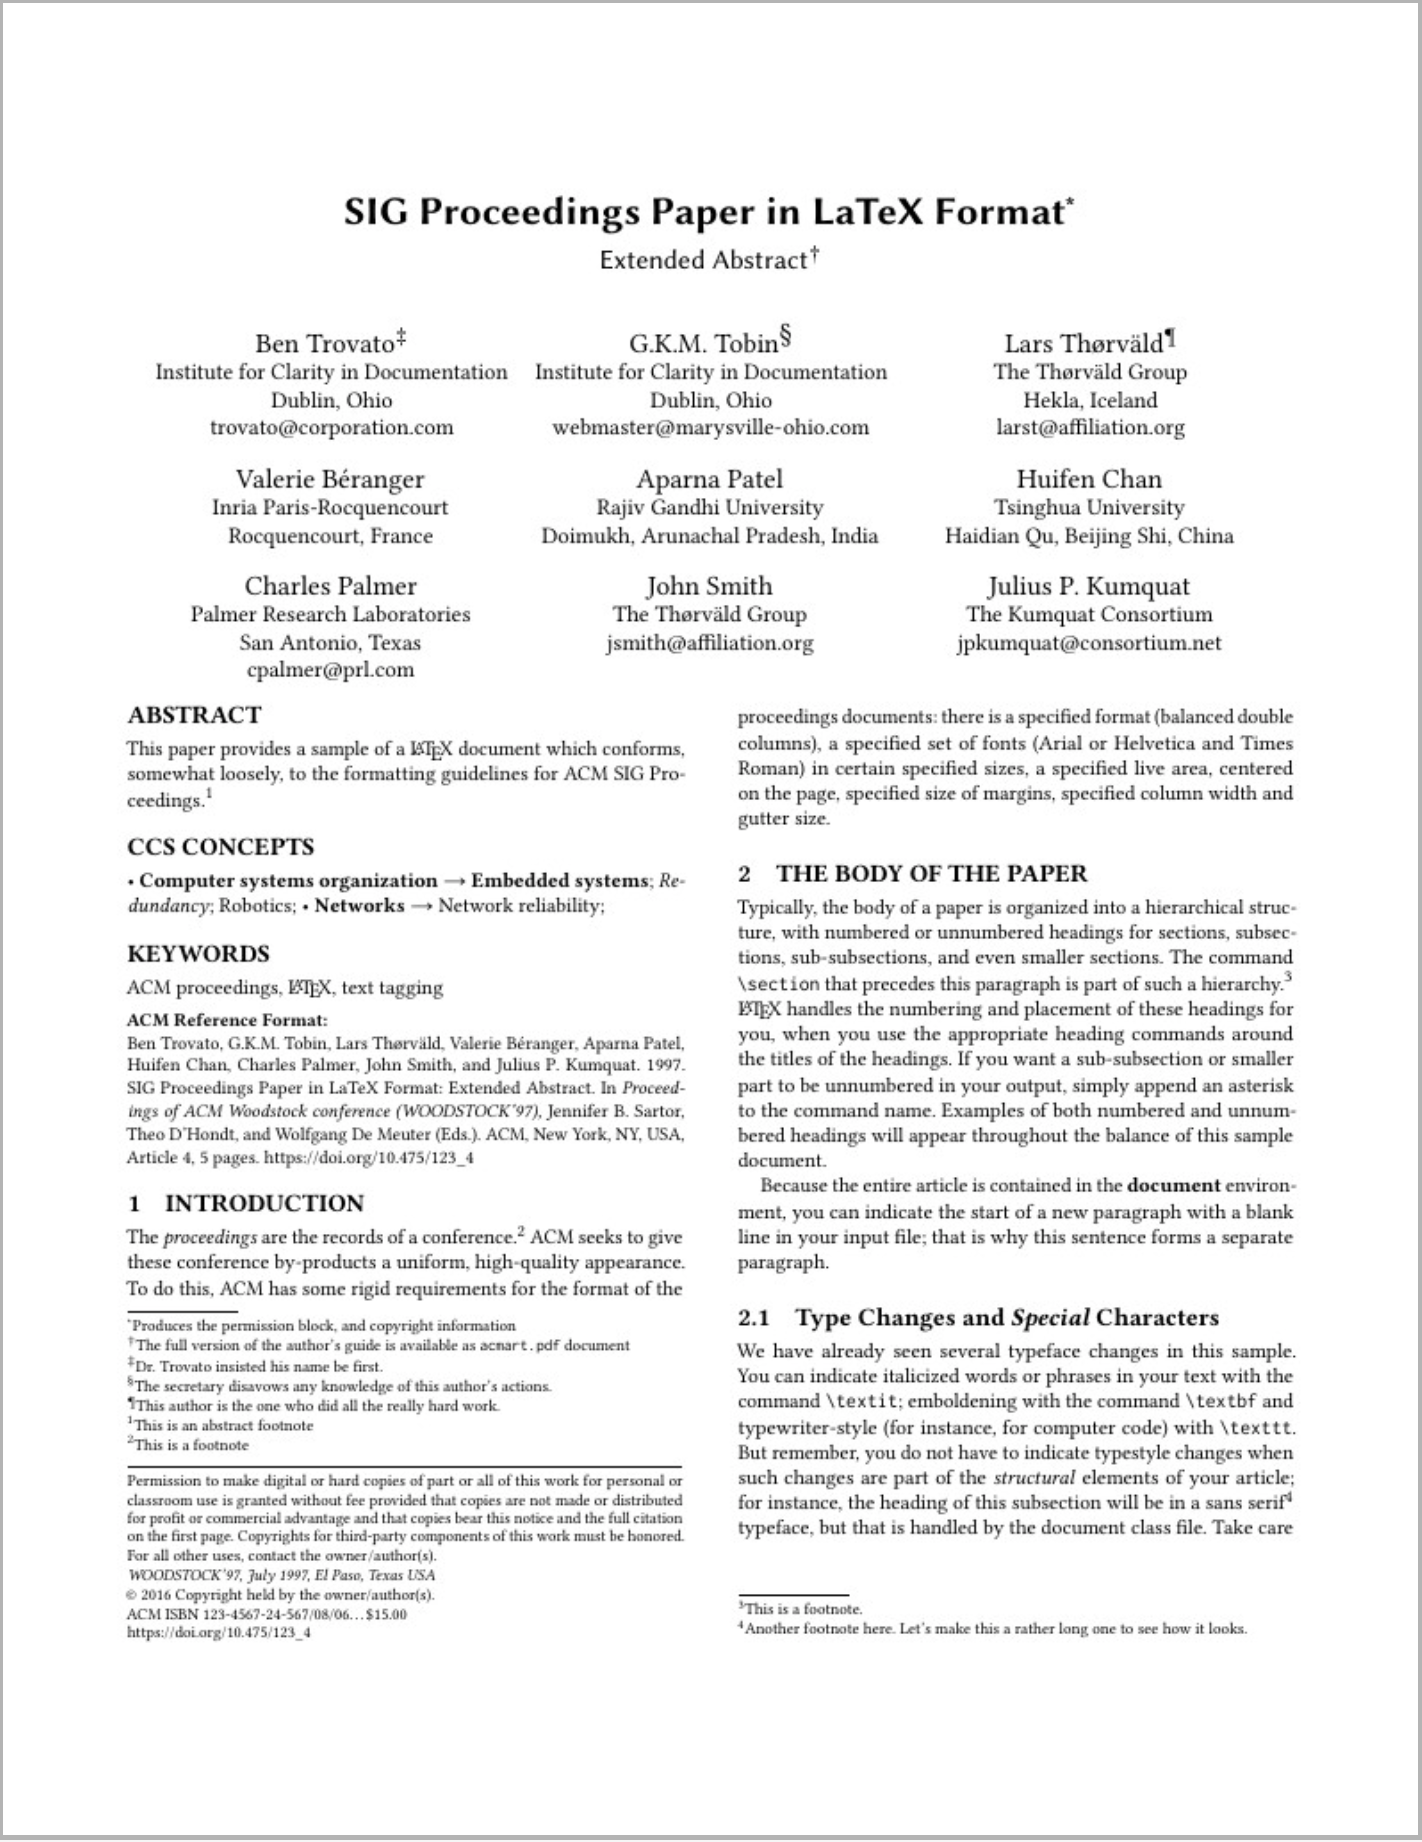
\includegraphics[width=6cm]{images/doc/acm.png}
  \hfill
  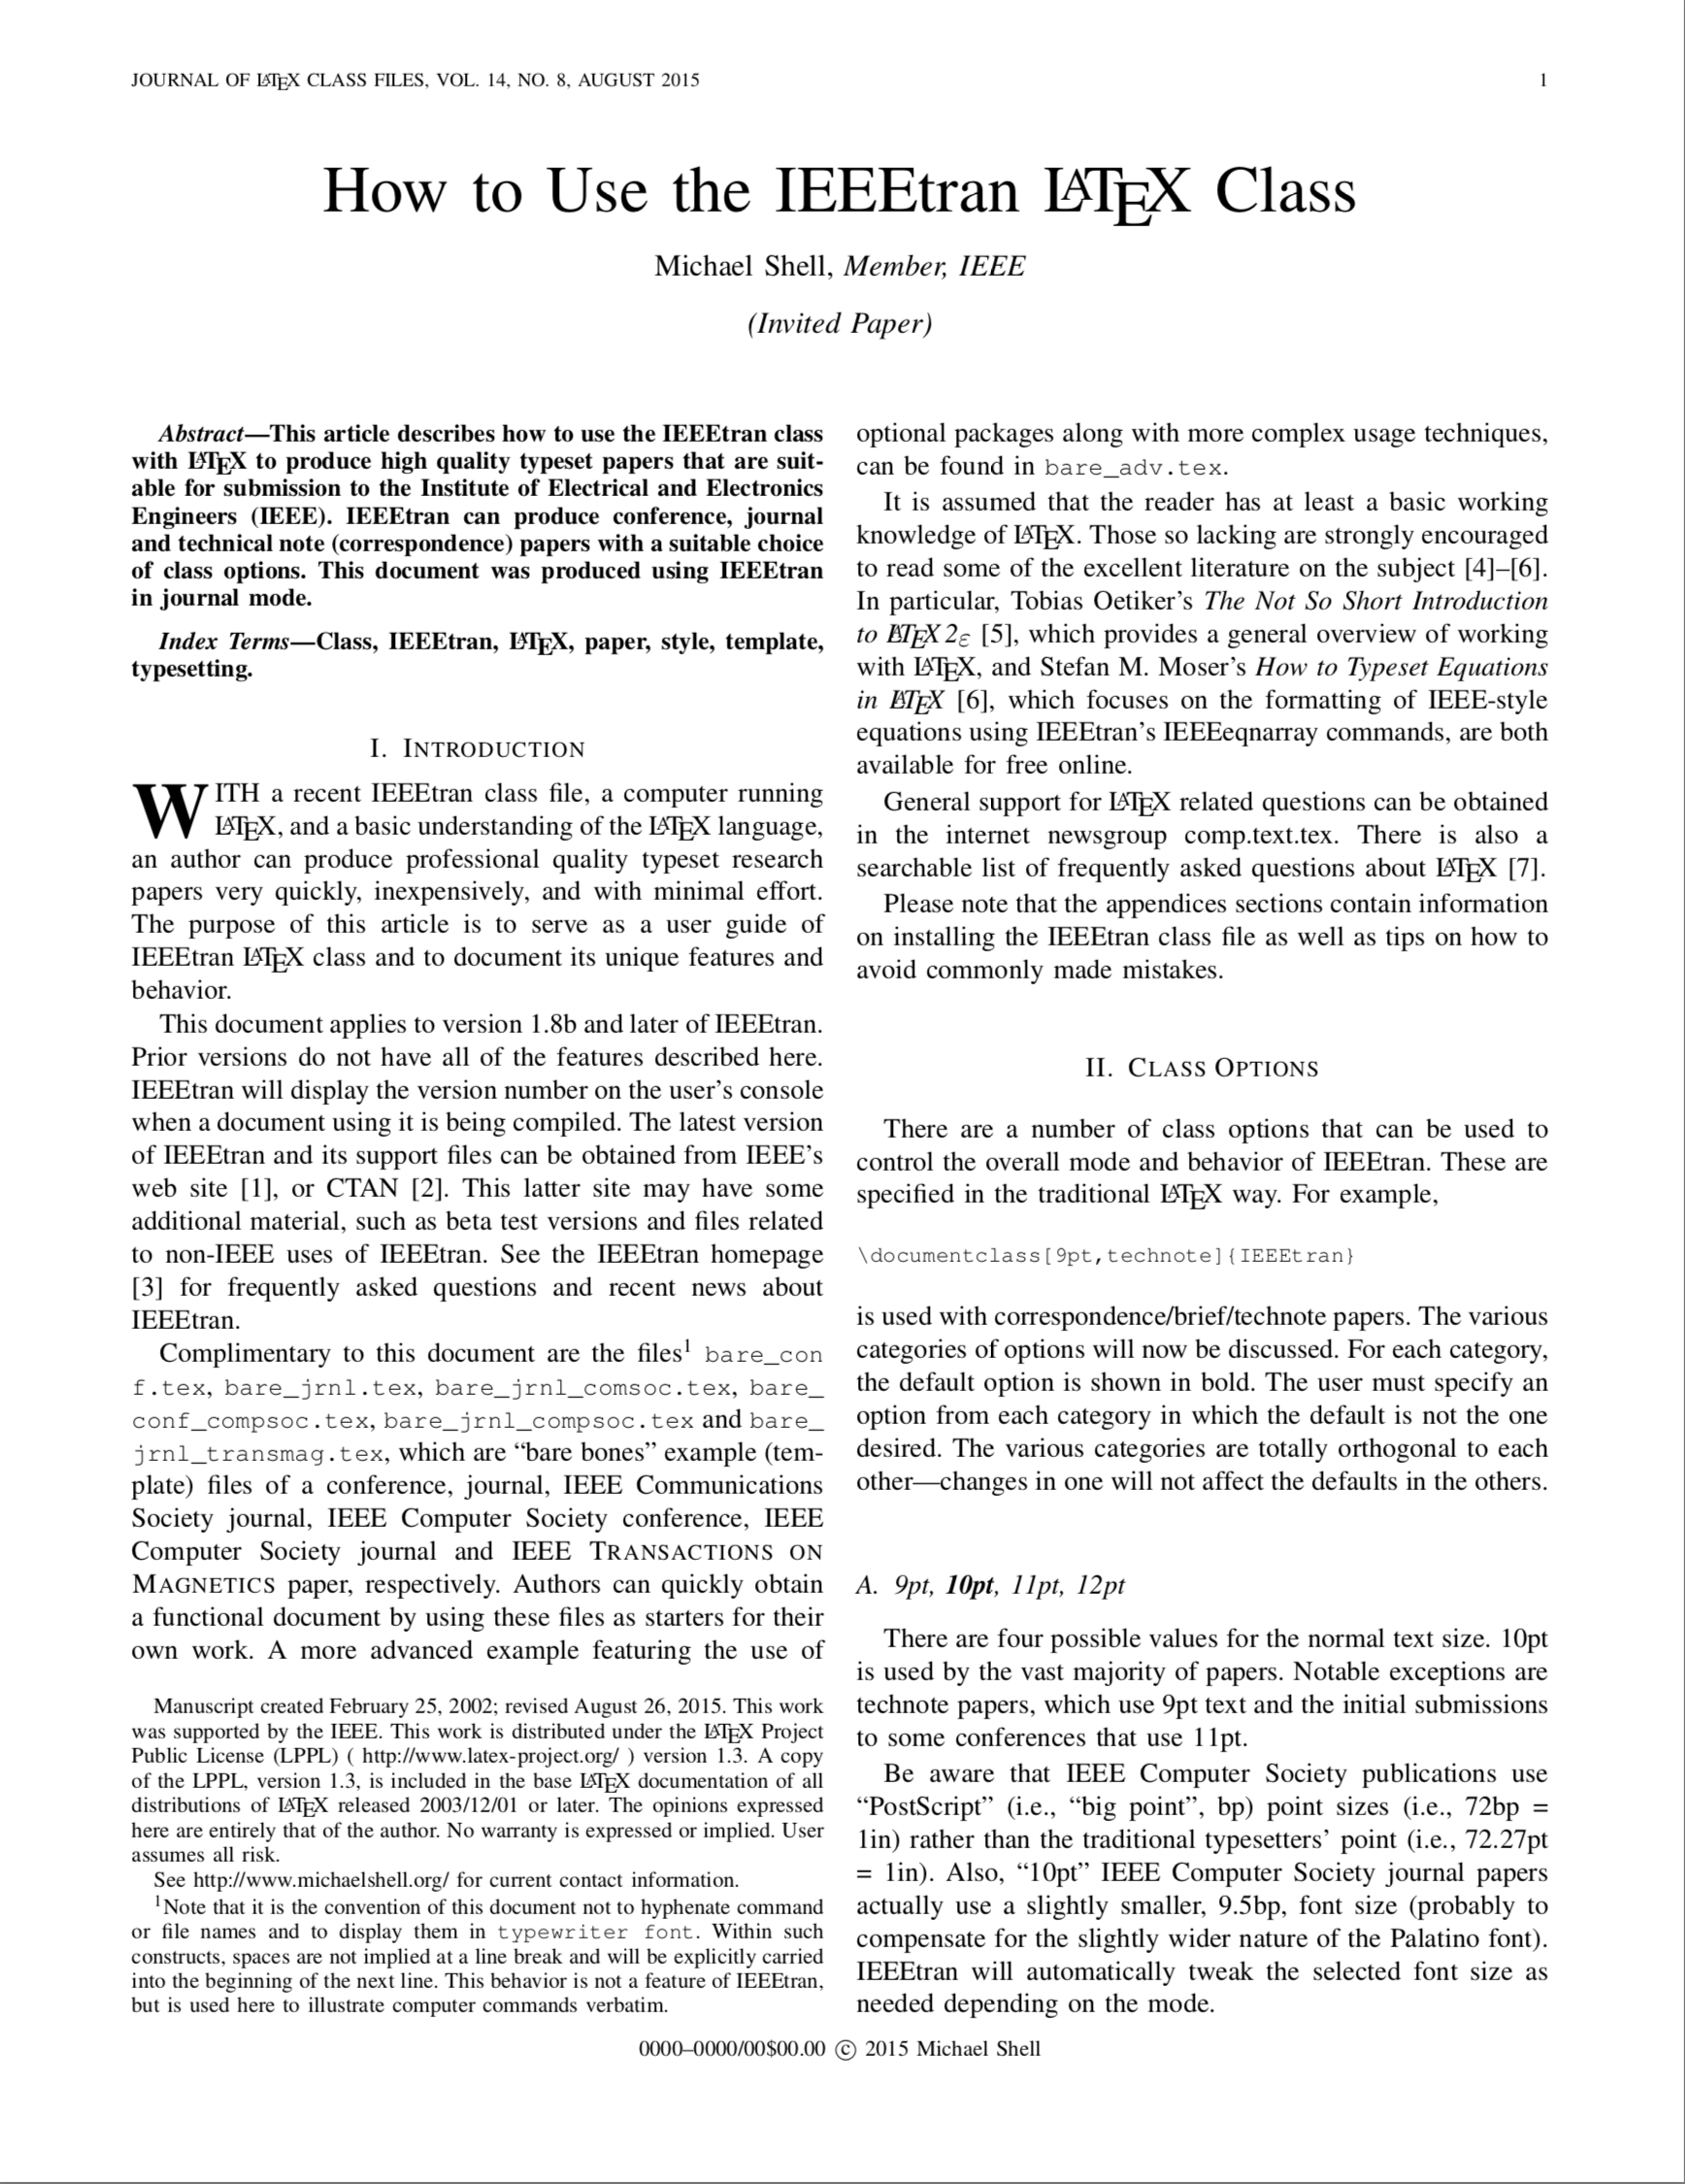
\includegraphics[width=6cm]{images/doc/ieee.png}
\caption{The look of the ACM and IEEE format templates}
\end{figure}

\begin{itemize}

\item
  \url{http://www.acm.org/publications/proceedings-template}
\item
  \url{https://www.ieee.org/conferences_events/conferences/publishing/templates.html}
\end{itemize}

\subsection{Generating and Managing Images}\label{generating-images}

To produce high quality images the programs PowerPoint and omnigraffle
on OSX are recommended. When using powerpoint please keep the image
ratio to 4x3 as they produce nice size graphics which you also can use
in your presentations. When using other rations they may not fit in
presentations and thus you may increase unnecessarily your work. We do
not recommend vizio as it is not universally available and produces
images that in case you have to present them in a slide presentation
does not easily reformat if you do not use 4x3 aspect ratio.

Naturally, graphics should be provided in SVG or PDF format so they can
scale well when we look at the final PDF. Including PNG, gif, or jpeg
files often do not result in the necessary resolution or the files
become real big. For this reason we for example can also not recommend
tools such as tablaeu as they do not provide proper exports to high
quality publication formats. For interactive display such tool may be
good, but for publications it produces inferior formatted images.

We recommend that all images be stored into a folder called images in
the same directory where your \LaTeX main document resides.


\subsection{Slides}\label{slides}
\index{Latex!slides}

Slides are best produced with the seminar package:

\begin{verbatim}
\documentclass{seminar}

\begin{slide}

    Hello World on slide 1

\end{slide}

The text between slides is ignored

\begin{slide}

    Hello World on slide 2

\end{slide}
\end{verbatim}

However, in case you need to have a slide presentation we recommend you
use ppt. Just paste and copy content from your PDF or your LaTeX source
file into the ppt.


\subsection{Useful Online Information about \LaTeX }
\index{Latex!other documentation}

\begin{description}


\item[Latex Sheet:]    \url{https://wch.github.io/latexsheet/latexsheet.pdf}

\item[Latex Short:]    \url{http://tug.ctan.org/info/lshort/english/lshort.pdf}

\item[Wikibook:]       \url{https://en.wikibooks.org/wiki/LaTeX}
\item[Wikibook (PDF)]: \url{https://upload.wikimedia.org/wikipedia/commons/2/2d/LaTeX.pdf}

\item [Links to books:] \url{https://latexforhumans.wordpress.com/2008/10/11/the-best-guides-to-latex/}
\item [Links to books:] \url{https://www.latex-project.org/help/books/}
\item [LaTeX2e:]
  The
  \href{http://texdoc.net/texmf-dist/doc/latex/latex2e-help-texinfo/latex2e.pdf}{LaTeX
  Reference Manual} provides a good introduction to Latex.

\end{description}


\begin{itemize}

\item
  LaTeX Users and Reference Guide, by Leslie Lamport
  \url{https://www.amazon.com/LaTeX-Document-Preparation-System-2nd/dp/0201529831/ref=sr_1_2?s=books\&ie=UTF8\&qid=1507114870\&sr=1-2\&keywords=lamport}
\item
  LaTeX an Introduction, by Helmut Kopka
  \url{https://www.amazon.com/Guide-LaTeX-4th-Helmut-Kopka/dp/0321173856/ref=pd_lpo_sbs_14_t_0?_encoding=UTF8\&psc=1\&refRID=2BB4APDFEX34A4JM65ZB}
\item
  The LaTeX Companion, by Frank Mittelbach
  \url{https://www.amazon.com/LaTeX-Companion-Techniques-Computer-Typesetting/dp/0201362996}
\end{itemize}



\subsection{LaTeX vs. X}\label{latex-vs.-x}

We will refrain from providing a detailed analysis on why we use LaTeX
in many cases versus other technologies. In general, we find that LaTeX:

\begin{itemize}
\tightlist
\item
  is incredibly stable
\item
  produces high-quality output
\item
  is platform independent
\item
  has lots of templates
\item
  has been around for many years so it works well
\item
  removes you from the pain of figure placements
\item
  focusses you on content rather tan the appearance of the paper
\item
  integrates well with code repositories such as git to write
  collaborative papers.
\item
  has superior bibliography integration
\item
  has a rich set of tools that make using LaTeX easier
\item
  authors do not play with layouts much so papers in a format are
  uniform
\end{itemize}

In case you need a graphical view to edit LaTeX or LateX exportable
files you also find AucTeX and Lyx.

\subsubsection{Word}\label{word}

Word is arguably available to many, but if you work on Linux you may be
out of luck. Also Word often focusses not on structure of the text but
on its appearance. Many students abuse Word and the documents in Word
become a pain to edit with multiple users. Recently Microsoft has
offered online services to collaborate on writing documents in groups
which work well. Integration with bibliography managers such as endnote
or Mendeley is possible.

However, we ran into issues whenever we use word:

\begin{itemize}
\tightlist
\item
  Word tends sometimes to crash for unknown reasons and we lost a lot of
  work
\item
  Word has some issues with the bibliography managers and tends to crash
  sometimes for unknown reasons.
\item
  Word is slow with integration to large bibliographies.
\item
  Figure placement in Word in some formats is a disaster and you will
  spend many hours to correct things just to find out that if you make
  small changes you have to spend additional many hours to get used to
  the new placement. We have not yet experienced a word version where we
  have not lost images. Maybe that has changed, so let us know
\end{itemize}

However, we highly recommend the collaborative editing features of Word
that work on a paragraph and not letter level. Thus saving is essential
so you do not block other people from editing the paragraph.

\subsubsection{Google Docs}\label{google-docs}

Unfortunately, many useful features got lost in the new google docs.
However, it is great to collaborate quickly online, share thoughts and
even write your latex documents together if you like (just copy your
work in a file offline and use latex to compile it ;-) )

The biggest issue we have with Google Docs is that it does not allow the
support of 2 column formats, that the bibliography integration is
non-existent and that paste and copy from web pages and images
encourages unintended plagiarism when collecting information without
annotations (LaTeX and Word are prone to this too, but we found from
experience that it tends to happen more with Google docs users.

\subsubsection{A Place for Each}\label{a-place-for-each}

When looking at the tools we find a place for each:

\begin{description}
\item[Google docs:]
Short meeting notes, small documents, quick online collaborations to
develop documents collaboratively at the same time.
\item[Word:]
Available to many, supports 2 column format, supports paragraph based
collaborative editing, Integrates with bibliography managers.
\item[LaTeX:]
Reduces failures, great offline editing, superior bibliography
management, superior image placement, runs everywhere. Great
collaborative editing with sharelatex, allows easy generation of
proceedings written by hundreds of people with shared index.
\item[The best choice for your class:]
LaTeX
\end{description}

\section{Editing}\label{editing}

\subsection{Emacs}\label{emacs}

The text editor emacs provides a great basis for editing TeX and LaTeX
documents. Both modes are supported. In addition there exists a color
highlight module enabling the color display of LaTeX and TeX commands.
On OSX aquaemacs and carbon emacs have build in support for LaTeX. Spell
checking is done with flyspell in emacs.

\subsubsection{Aquamacs}

Aquamacs is an editor based on GNU Emacs that runs on OSX and
integrates with the OSX desktop. This is for many the preferred editor
on OSX for \LaTeX.

\url{http://aquamacs.org}

\begin{figure}[!h]
  \centering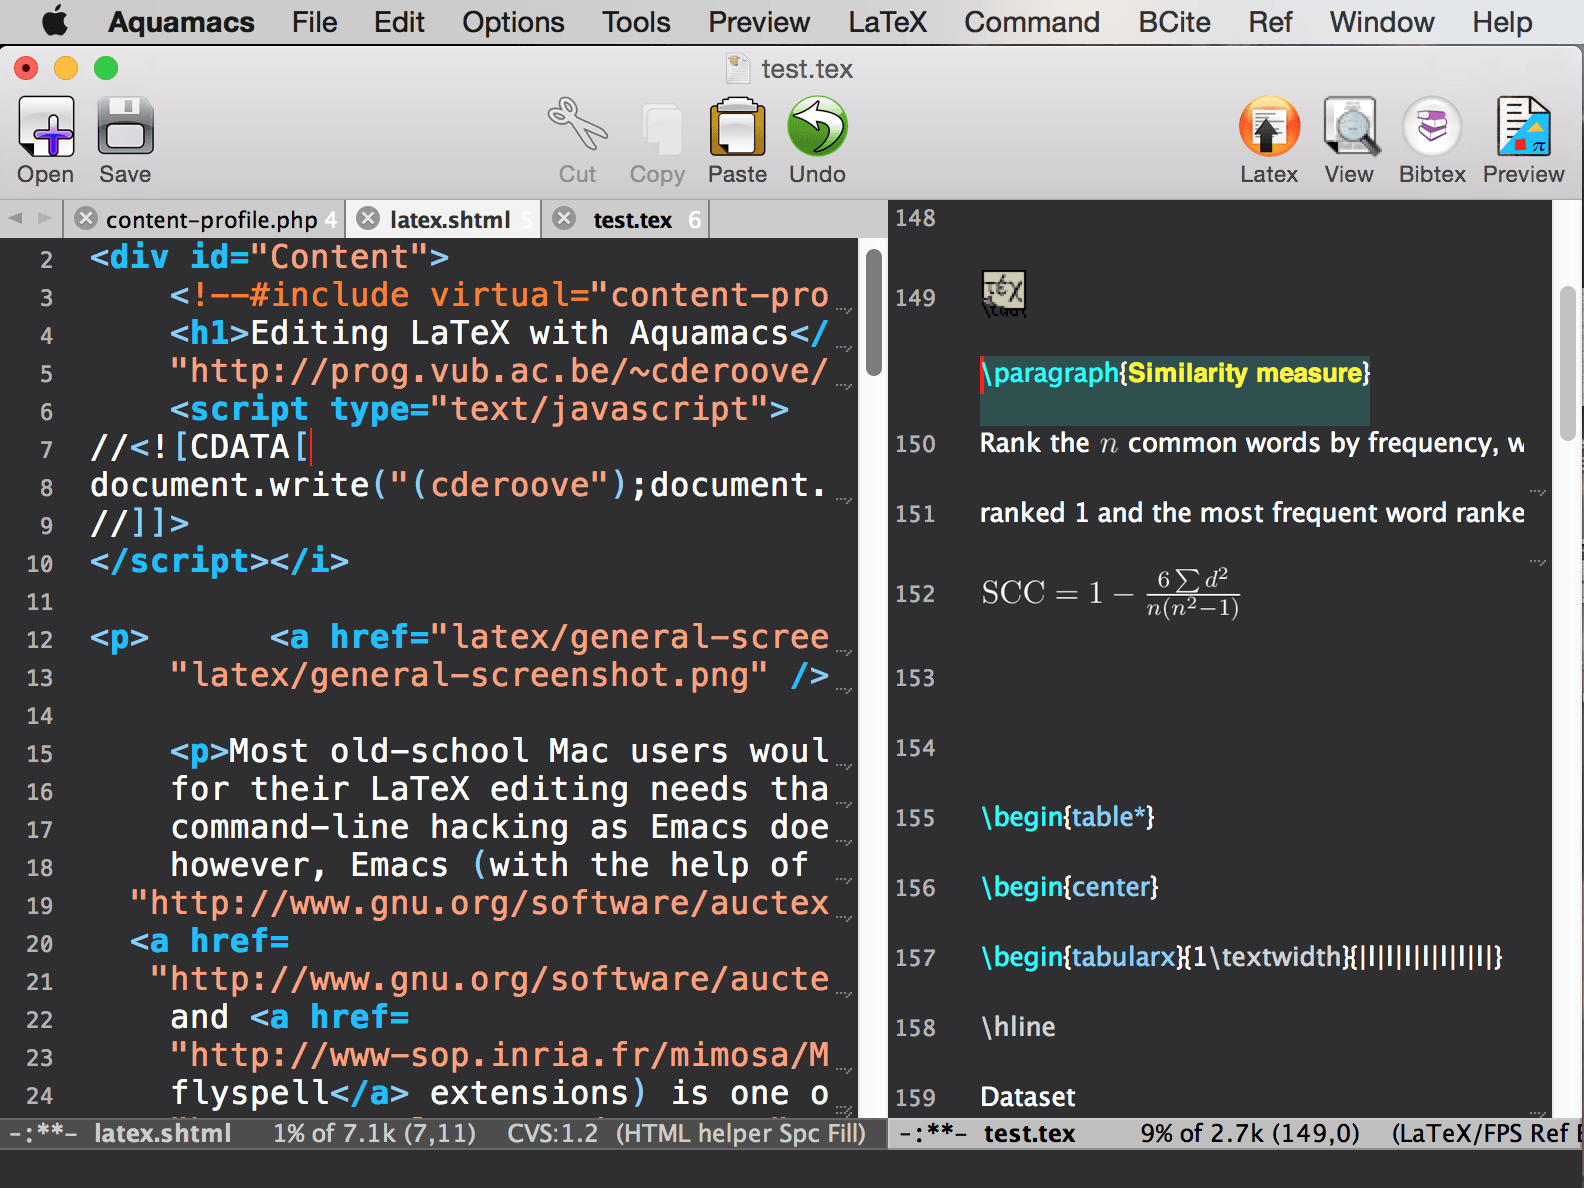
\includegraphics[width=8cm]{images/aquamacs.png}
  \caption{Aquamacs}
  \label{F:aquamacs}
\end{figure}


\subsection{Vi/Vim}\label{vivim}

Another popular editor is vi or vim. It is less feature rich but many
programmers ar using it. As it can edit ASCII text you can edit LaTeX.
With the LaTeX add-ons to vim, vim becomes similar powerful while
offering help and syntax highlighting for LaTeX as emacs does. (The
authors still prefer emacs)

\subsection{TeXshop}\label{texshop}

Other editors such as TeXshop are available which provide a more
integrated experience. However, we find them at times to stringent and
prefer editors such as emacs.

\subsection{LyX}\label{lyx}

We have made very good experiences with Lyx. You must assure that the
team you work with uses it consistently and that you all use the same
version.

\begin{figure}[!h]
  \centering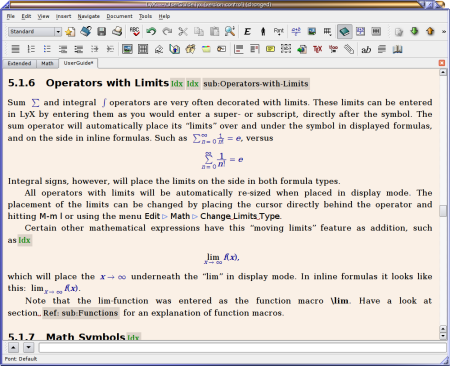
\includegraphics[width=8cm]{images/lyx.png}
  \caption{Lyx}
  \label{F:lyx}
\end{figure}

Using the ACM templates is documented here:

\begin{itemize}
\tightlist
\item
  \url{https://wiki.lyx.org/Examples/AcmSiggraph}
\end{itemize}

On OSX it is important that you have a new version of LaTeX and Lyx
installed. As it takes up quite some space, you ma want to delete older
versions. The new version of LyX comes with the acmsigplan template
included. However on OSX and other platforms the .cls file is not
included by default. However the above link clearly documents how to fix
this.

\subsection{WYSIWYG locally}\label{wysiwyg-locally}

We have found that editors such as Lyx and Auctex provide very good
WYSIWYG alike features. However, we found an even easier way while using
skim, a pdf previewer, in conjunction with emacs and latexmk. This can
be achieved while using the following command assuming your latex file
is called `report.tex`:

\begin{verbatim}
latexmk -pvc -view=pdf report
\end{verbatim}

This command will update your pdf previewer (make sure to use skim)
whenever you edit the file report.tex and save it. It will maintain via
skim the current position, thus you have a real great way of editing in
one window, while seeing the results in the other.

Skim can be found at: \url{http://skim-app.sourceforge.net/}

\subsection{Markdown and \LaTeX}
\index{Latex!markdown}

It may come as a surprise to many that one can actually write simple
LaTeX documents also in markdown Syntax or mix section written in
markdown while others are written in LaTeX. To do so all you ahve to
do is place the markdown text in a separate file. Let us call the file 
\verb|content.md| which has the following lines included in it:

\begin{verbatim}
# Section

* item a
* item b
\end{verbatim}

Obviously, we would have to convert this to LaTeX. Luckily there is a
very useful program called {\em pandoc} that does this for you. YOu
could make the translation in the shell, but you could also make the
translation locally on your computer while allowing \LaTeX to start up
external programs. This is achieved with the {\em write18} command and
allowing LaTeX explicitly to call external programs. Please inspect
the following latex file that includes a template on how to do
this. We assume the file is called markdown.tex for our example.

\begin{verbatim}
\documentclass{article}

\include{graphicx}
\newcommand{\tightlist}{}

\begin{document}
\immediate\write18{pandoc content.md -o content.tex}

\input{content}

\end{document}
\end{verbatim}

Now to generate the PDF we simply have to call the following command
that include the {\em -shell-escape} flag to allow the execution of
write18 embedded commands:

\begin{verbatim}
pdflatex -shell-escape markdown-test
\end{verbatim}

The output will be {\em markdown.pdf} with the content from the
markdown file translated. Doing this naturally allows you to write
large portions in markdown and automatically include them in your
LaTeX document. Hence, you can use editors such as Macdown to initially
work in semi WYSIWYG mode and do fairly straight forward
edition. Naturally the same can be done in RST. Naturally the most
elementary features are supported. For more sophisticated features,
please use LaTeX directly.


\subsection{Including RST into LaTeX}

content.rst:

\begin{verbatim}
Section
-------

* item a
* item b
\end{verbatim}

sample.tex:

\begin{verbatim}
\documentclass{article}

\include{graphicx}
\newcommand{\tightlist}{}

\begin{document}
\immediate\write18{pandoc content.rst -o content.tex}

\input{content}

\end{document}
\end{verbatim}


\subsection{pyCharm}

TODO: comment on how we can use pycharm for editing and what the
limitations are.

\subsection{MSWord}

it is possible to use Word.

be careful with 

\section{The LaTeX Cycle}\label{the-latex-cycle}
\index{Latex!cycle}

To create a PDF file from latex yo need to generate it following a
simple development and improvement cycle.

First, Create/edit ASCII source file with \texttt{file.tex} file:

\begin{verbatim}
emacs file.tex
\end{verbatim}

Create/edit bibliography file:

\begin{verbatim}
jabref refs.bib
\end{verbatim}

Create the PDF:

\begin{verbatim}
pdflatex file
bibtex file
pdflatex file
pdflatex file
\end{verbatim}

View the PDF:

\begin{verbatim}
open file
\end{verbatim}

It not only showcases you an example file in ACM 2 column format, but
also integrates with a bibliography. Furthermore, it provides a sample
Makefile that you can use to generate view and recompile, or even
autogenerate. A compilation would look like:

\begin{verbatim}
make
make view
\end{verbatim}

If however you want to do things on change in the tex file you can do
this automatically simply with:

\begin{verbatim}
make watch
\end{verbatim}

for make watch its best to use skim as pdf previewer


\section{Tips}\label{tips}

Including figures over two columns:

\begin{itemize}
\item
  \url{http://tex.stackexchange.com/questions/30985/displaying-a-wide-figure-in-a-two-column-document}
\item
  positioning figures with textwidth and columnwidth
  \url{https://www.sharelatex.com/learn/Positioning_images_and_tables}
\item
  An organization as the author. Assume the author is National Institute
  of Health and want to have the author show up, please do:

\begin{verbatim}
key= {National Institute of Health},
author= {{National Institute of Health}},
\end{verbatim}

  Please note the \{\{ \}\}
\item
  words containing `fi' or `ffi' showing blank places like below after
  recompiling it: find as nd efficiency as e ciency

  You copied from word or PDF ff which is actually not an ff, but a
  condensed character, change it to ff and ffi, you may find other such
  examples such as any non ASCII character. A degree is for example
  another common issue in data science.
\item
  do not use \textbar{} \& and other latex characters in bibtex
  references, instead use , and the word and
\item
  If you need to use \_ it is \_ but if you use urls leave them as is
\item
  We do recommend that you use sharelatex and jabref for writing papers.
  This is the easiest solution and beats in many cases MSWord as you can
  focus on writing and not on formatting.
\end{itemize}

\subsection{Colorful Output}

Instead of using pdflatex, you can also install \verb|pydflatex| that
provides a convenient wrapper and colorizes the output while
eliminating a lot of warnings that you may initially not want to deal
with. To install it please use:

\begin{verbatim}
pip install blessings
pip install -e "git+https://github.com/olivierverdier/pydflatex#egg=pydflatex"
\end{verbatim}

You can see the manula page with 

\begin{verbatim}
pydflatex --help

usage: usage: pydflatex [options] texfile1

Compile a tex file with pdflatex and make the auxiliary files invisible. Note
that the '.tex' extension may be omitted

positional arguments:
  tex path            path to tex file

optional arguments:
  -h, --help          show this help message and exit
  -o, --open          view the pdf file(s) in a pdf viewer.
  -k, --continue      continue on error
  -w, --with-warning  do not suppress common warnings
  -v, --verbose       Verbose output for debugging
  -p, --plain         No coloured output
  -x, --xetex         Use XeLaTeX engine
  -l, --log-parsing   Only parse log
  -t, --typesetting   Only typeset
\end{verbatim}

%============================================================
\chapter{Managing Bibliographies}
\label{C:bibtex}
%============================================================

\FILENAME

\section{Integrating Bibliographies}
\label{S:bibliographies}
\index{Bibliography}
\index{bibtex}
\index{biber}

Bibliography management in \LaTeX\ is one of the many features that
motivate many researchers to make \LaTeX the tool of choice to write
academic papers. There are numerous bibliography styles available that
allow easy adaptation to differen journal and proceedings style. As
such, it includes styles for bibliographies formated in ACM and IEEE
style.

\subsection{biber}

\TODO{Describe use of biber instead of bibtex}

\subsection{bibtex}

This section assumes we use the standard bibtex program to integrate
citations into a \LaTeX\ paper.

An example to use the IEEE style for a paper includes to set
the style to IEEEtran before you add the reference:

\begin{verbatim}
\bibliographystyle{IEEEtran}
\bibliography{references.bib}
\end{verbatim}

To properly create PDF papers which using bibtex, we have to make sure
that all indexes, citations, references and labels are updated. This
is done with the help of the following commands assuming your file is
called \verb|file.tex|

\begin{verbatim}
pdflatex  file
bibtex file
pdflatex  file
pdflatex  file
\end{verbatim}


\begin{IU}
At IU you are required to use our template. which includes a Makefile
and either calls the above three commands or used latexmk
\end{IU}

The reason for the multiple execution of the latex program is to update
all cross-references correctly. In case you are not interested in
updating the library every time in the writing progress just postpone it
till the end. Missing citations are viewed as {[}?{]}.

Two programs stand out when managing bibliographies: emacs and jabref:

  \URL{http://www.jabref.org/}

Other programs such as Mendeley, Zotero, and even endnote integrate with
bibtex. However their support is limited, so we recommend that you just
use jabref as it is free and runs on all platforms.

\subsection{jabref}\label{jabref}

\TODO{Tyler: include cite for jabref, bibtex, biber at appropriate
  location in this section. Add them to the bib file.}

Practical experience with many generations of students shows that
\textit{jabref} is a very simple to use bibliography manager for LaTeX and
other systems. It can create a multitude of bibliography file formats
and allows upload in other online bibliography managers.

For information on how to install and use jabref please go to 
\url{http://www.jabref.org/}. There you will find the appropriate
download link.

We provide also a convenient video on how to use jabref and show
several methods on how to add entries easily to your bibliography database.

\video{Bibliography}{1:41}{jabref}{https://youtu.be/QVbifcLgMic}



\section{Entry types}

In this section we will explain how to find and properly generate
bibliographic entries. We are using bibtex for this as it is easy to
use and generates reasonable entries that can be included in
papers. What we like to achieve in this section is not to just show
you a final entry, but to document the process on how that entry was
derived. This will allow you to replicate or learn from the process to
apply to your own entries. As part of this we copy and paste
information found via Web searches.

We will address a number of important reference types which includes:

\begin{itemize}

\item
  wikipedia entries
\item
  github (see Section~\ref{s:e:source-code-references})
\item
  books
\item
  articles in a scientific journal (see Section~\ref{s:e:article-in-a-journal})
\item
  articles in a conference (see Section~\ref{s:e:article-in-a-conference-proceedings})
\item
  articles in magazines (non scientific)
\item
  blogs
\end{itemize}

\subsection{Source Code References}
\label{s:e:source-code-references}
\index{Bibtex!Source code}

Often, we need to cite a source code from a publicly hosted
repository. Such repositories are frequently used and include, for
example github, bitbucket, sourceforge, or your Universities code
repository as long as it is publicly reachable. As changes can occur on
these repositories, it is important that the date of access is listed in
the entry or even the release version of the source code.

Let us without bias chose a random source dode entry that has been
contributed by a student as follows:

\begin{verbatim}
@Misc{gonzalez_2015,
  Title =  {Buildstep},
  Author =     {Gonzalez, Jose and Lindsay, Jeff},
  HowPublished = {Web Page},
  Month =  {Jul},
  Note =   {Accessed: 2017-1-24},
  Year =   2015,
  Key =        {www-buildstep},
  Url =        {https://github.com/progrium/buildstep}
}
\end{verbatim}

Is this entry correct? Let us analyse. But first we need to undersrand
the semantics of the fields.

\subsubsection{What are the Different entry Types and Fields}

You see that the entry contains a number of fields. An extensive
explanation of these fields can be found at 

Please see \url{https://en.wikipedia.org/wiki/BibTeX}

We provide for this example a comprehensive discussions of the fields
used. For other examples we suggest you refer to the document to
identify what needs to be filled out.

\subsubsection{Entry type Misc}\label{s:e:entry-type-misc}
\index{Bibtex!Field!Misc}

First, it seems appropriate to use a \emph{@misc} entry. We correctly
identify this is a misc entry as it is online available. More recent
version of bibtex include also the type \emph{@online} for it. However,
in order to maintain compatibility to older formats we chose simply Misc
here and if we really would need to we could replace it easily.

\subsubsection{Label}\label{s:e:label}
\index{Bibtex!Field!Label}

Typically the bibliography label should contain 3 letters from an
author name, short year and the short name of the publication to
provide maximum information regarding the publication. However in this
case the project is hosted on github, so creating the label based on
just the github location seems more logical. Thus our label that we
propose is given by 

\verb|github-progrium-buildstep|


Under no circumstances should you use underscores as they can have unintended
consequences in programs we use to create papers for our classes. Just
use a minus sign instead. As it is hosted on github we also want the
githubname and the projectname. As you can see we just derived it from
the URL.

\begin{IU}
When managing bibliography entries with large numbers of collaborators
it is advisable that all bibliography labels be initially be prefixed
with an id for the collaborator. In our case we use the HID. Thus in
our case we will have the following label.

\verb|hid-sp18-000-github-progrium-buildstep|

\end{IU}


\subsubsection{Author}\label{s:e:author}
\index{Bibtex!Field!Author}

Normally we can write in the author fiels the names of the authors
separated by the work and. IT is important tu use the word \verb|and|
but not use a comma. However, this only works if the lastname does not
contain a space in it. In order to avoid confusing the system, we
recommend therefore to write all names in the form
\verb|Lastname, Firstname Middle Initials|

Thus we find in our example

\verb|  Author =     {Gonzalez, Jose and Lindsay, Jeff},|

\begin{WARNING}
Please note the word and between authors. and not a comma, commas are
only used to distinguish between lastname and firstname.
\end{WARNING}


\subsubsection{Key}\label{s:e:key}
\index{Bibtex!Field!Key}

In this case the key field can be removed as the entry has an author
field entry. If there was no author field, we use the key to specify
the alphabetical ordering based on the specified key. Note that a key is
not the label. In fact in our original entry the key field was wrongly
used and the student did not understand that the key is used for
sorting.

\subsubsection{Howpublished}\label{s:e:howpublished}
\index{Bibtex!Field!Howpublished}

Since the source is a github project repository, the howpublished field
shall hold the value \verb|{Code Repository}|. If the
url specified was a normal webpage, the \verb|{Web Page}| entry would be
valid.

\subsubsection{Month}\label{s:e:month}
\index{Bibtex!Field!Month}

To allow internationalization of the month we use the first 3 letters
in the english language for the month. Thus it is 
\verb|month = jul|. Note that there are no brackets around the month.

\subsubsection{Owner}\label{s:e:owner}
\index{Bibtex!Field!Owner}

In class we introduced the convention to put the student HID in it. If
multiple students contributed, add them with space separation.

\subsubsection{Accessed}\label{s:e:accessed}
\index{Bibtex!Field!Accessed}

As some styles do not support the accessed field, we simply include it in
the note field. This is absolutely essential as code can change and when
we read the code we looked at a particular snapshot in time. In addition
it is often necessary to record the actual version of the code or the branch.
Typically for github entries, it is best to just use the month and
year field as some styles check for it.

\subsubsection{Final Entry}

Filling out as many fields as possible with information for this entry
we get:

\begin{verbatim}
@Misc{github-progrium-buildstep,
  Title =  {Buildstep},
  Author =     {Jose Gonzalez and Jeff Lindsay},
  HowPublished = {Code Repository},
  Year =   {2015},
  Month =  jul,
  Note =   {Accessed: 2017-1-24, master branch},
  Url =    {https://github.com/progrium/buildstep},
  Owner =  {S17-IO-3025},
}
\end{verbatim}

We are using the release date in the year and month field as this
project uses this for organizing releases. However, other project may
have release versions so you would have in addition to using the data
also to include the version in the note field such as:

\begin{verbatim}
Note =     {Version: 1.2.3, Accessed: 2017-1-24},
\end{verbatim}


\subsection{Pedigree}

Often it is advantageous to document the pedigree of the bibtex
entries. Eg, how did you derive the final entry? To do so you can
simply add a field such as \verb|bibsource| and include in it all
links you used to gather the final entry. However, we believe that the
effort to curate an entry is sufficient to manage your own
bibliography which you should freely distribute and constitute an own
contribution. 

\subsection{Article in a Journal}
\label{s:e:article-in-a-journal}
\index{Bibtex!Article}

Many online bibtex entries that you will find are wrong or
incomplete. Often you may find via google a bibtex entry that may need
some more research. Let us assume your first google query returns a
publication and you cite it such as this:

\begin{verbatim}
@Unpublished{unpublished-google-sawzall,
    Title = {{Interpreting the Data: Parallel Analysis with Sawzall}},
    Author = {{Rob Pike, Sean Dorward, Robert Griesemer, Sean Quinlan}},
    Note = {accessed 2017-01-28},
    Month = {October},
    Year = {2005},
    Owner = {for the purpose of this discussion removed},
    Timestamp = {2017.01.31}
}
\end{verbatim}

Could we improve this entry to achieve your best? We observe:

\begin{enumerate}
\item
  The author field has a wrong entry as the \verb|,| is to be replaced by an
  \verb|and|.
\item
  The author field has authors and thus must not have a \{\{ \}\}
\item
  The url is missing, as the simple google search actually finds a PDF
  document.
\end{enumerate}

Let us investigate a bit more while searching for the title. We find

\begin{enumerate}
\def\labelenumi{\Alph{enumi}}
\item
  \url{https://www.google.com/url?sa=t\&rct=j\&q}=\&esrc=s\&source=web\&cd=1\&ved=0ahUKEwj\_ytSA-PDRAhUH8IMKHaomC-oQFggaMAA\&url=https\%3A\%2F\%2Fresearch.google.com\%2Farchive\%2Fsawzall-sciprog.pdf\&usg=AFQjCNHSSfKBwbxVAVPQ0td4rTjitKucpA\&sig2=vbiVzi36B3gGFjIzlUKBDA\&bvm=bv.146073913,d.amc
\item
  \url{https://research.google.com/pubs/pub61.html}
\item
  \url{http://dl.acm.org/citation.cfm?id=1239658}
\end{enumerate}

Let us look at (A)

As you can see from the url this is actually some redirection to a google
web page which probably is replaced by B as its from google research. So
let us look at (B)

Now when you look at the link we find the url
\url{https://research.google.com/archive/sawzall-sciprog.pdf} which
redirects you to the PDF paper.

When we go to (B) we find surprisingly a bibtex entry as follows:

\begin{verbatim}
@article{61,
  title = {Interpreting the Data: Parallel Analysis with Sawzall},
  author = {Rob Pike and Sean Dorward and Robert Griesemer and Sean Quinlan},
  year = 2005,
  URL = {https://research.google.com/archive/sawzall.html},
  journal = {Scientific Programming Journal},
  pages = {277--298},
  volume = {13}
}
\end{verbatim}

Now we could say let us be satisfied, but (C) seems to be even more
interesting as its from a major publisher. So lats just make sure we
look at (C)

If you go to (C), you find under the colored box entitled Tools and
Resources a link called \textbf{bibtex}. Thus it seems a good idea to
click on it. This will give you:

\begin{verbatim}
@article{Pike:2005:IDP:1239655.1239658,
    author = {Pike, Rob and Dorward, Sean and Griesemer, Robert and Quinlan, Sean},
    title = {Interpreting the Data: Parallel Analysis with Sawzall},
    journal = {Sci. Program.},
    issue_date = {October 2005},
    volume = {13},
    number = {4},
    month = oct,
    year = {2005},
    issn = {1058-9244},
    pages = {277--298},
    numpages = {22},
    url = {http://dx.doi.org/10.1155/2005/962135},
    doi = {10.1155/2005/962135},
    acmid = {1239658},
    publisher = {IOS Press},
    address = {Amsterdam, The Netherlands, The Netherlands},
}
\end{verbatim}

Now we seem to be at a position to combine our search result as neither
entry is sufficient. As the doi number properly specifies a paper (look
up what a doi is) we can replace the url with one that we find online,
such as the one we found in (A) Next we see that all field sin B are
already covered in C, so we take (C) and add the url. Now as the label is
great and uniform for ACM, but for us a bit less convenient as its
difficult to remember, we just change it while for example using
authors, title, and year information. let us also make sure to do mostly
lowercase in the label just as a convention. Thus our entry looks like:

\begin{verbatim}
@article{pike05swazall,
    author = {Pike, Rob and Dorward, Sean and Griesemer, Robert and Quinlan, Sean},
    title = {Interpreting the Data: Parallel Analysis with Sawzall},
    journal = {Sci. Program.},
    issue_date = {October 2005},
    volume = {13},
    number = {4},
    month = oct,
    year = {2005},
    issn = {1058-9244},
    pages = {277--298},
    numpages = {22},
    url = {https://research.google.com/archive/sawzall-sciprog.pdf},
    doi = {10.1155/2005/962135},
    acmid = {1239658},
    publisher = {IOS Press},
    address = {Amsterdam, The Netherlands, The Netherlands},
}
\end{verbatim}

As you can see properly specifying a reference takes multiple google
queries and merging of the results you find from various returns. As
you still have time to correct things I advise that you check your
references and correct them. If the original reference would have been
graded it would have been graded with a ``fail'' instead of a ``pass''.

Naturally you need to judge if you can integrate the URL or not, often
papers exist in a prepublication and you must make sure to cite the
version you used. IN fact if you have the prepublicAtion, you should
obtain the final manuscript as it could contain significant
corrections to the previous draft. In other cases the prepublication
may just be fine and you could for your own references keep the
url. FOr the final publication you probably want to make sure that the
doi is used. FOr the collection of your references, adding the url
could be useful.

\subsection{Article in a Conference Proceedings}
\label{s:e:article-in-a-conference-proceedings}
\index{Bibtex!InProceedings}

Now let us look at another obvious example that needs improvement:

\begin{verbatim}
@InProceedings{wettinger-any2api,
  Title      = {Any2API - Automated APIfication},
  Author     = {Wettinger, Johannes and
                Uwe Breitenb{\"u}cher
                and Frank Leymann},
  Booktitle  = {Proceedings of the 5th International
                Conference on Cloud Computing and
                Services Science},
  Year       = {2015},
  Pages      = {475­486},
  Publisher  = {SciTePress},
  ISSN       = {2326-7550},
  Owner      = {S17-IO-3005},
  Url        = {https://pdfs.semanticscholar.org/1cd4/4b87be8cf68ea5c4c642d38678a7b40a86de.pdf}
}
\end{verbatim}

As you can see this entry seems to define all required fields, so we
could be tempted to stop here. But its good to double check. Let us do
some queries against ACM and google scholar. Let us just type in the
title, and if this is in a proceedings they should return hopefully a
predefined bibtex record for us.

Let us query:

\begin{verbatim}
google: googlescholar Any2API Automated APIfication
\end{verbatim}

We get:

\begin{itemize}

\item
  \url{https://scholar.google.de/citations?view_op=view_citation\&hl=en\&user=j6lIXt0AAAAJ\&citation_for_view=j6lIXt0AAAAJ:8k81kl-MbHgC}
\end{itemize}

On that page we see
\href{https://scholar.google.com/scholar_lookup?title=Automated+drug+dispensing+system+reduces+medication+errors+in+an+intensive+care+setting\&author=Chapuis\&publication_year=2010\#}{Cite}

So we find a PDF at
\url{https://pdfs.semanticscholar.org/1cd4/4b87be8cf68ea5c4c642d38678a7b40a86de.pdf}

Let us click on this and the document includes a bibtex entry such as:

\begin{verbatim}
@inproceedings{Wettinger2015, 
  author= {Johannes Wettinger and Uwe Breitenb{\"u}cher and Frank
       Leymann},
  title = {Any2API - Automated APIfication},
  booktitle = {Proceedings of the 5th International Conference on Cloud
       Computing and Service Science (CLOSER)},
  year = {2015},
  pages = {475--486},
  publisher = {SciTePress}
} 
\end{verbatim}

Now let us add the URL and owner:

\begin{verbatim}
@inproceedings{Wettinger2015, 
  author= {Johannes Wettinger and Uwe Breitenb{\"u}cher and Frank
       Leymann},
  title = {Any2API - Automated APIfication},
  booktitle = {Proceedings of the 5th International Conference on Cloud
       Computing and Service Science (CLOSER)},
  year = {2015},
  pages = {475--486},
  publisher = {SciTePress},
  url ={https://pdfs.semanticscholar.org/1cd4/4b87be8cf68ea5c4c642d38678a7b40a86de.pdf},
  owner = {S17-IO-3005},
} 
\end{verbatim}

Should we be satisfied? No, even our original information we gathered
provided more information. So let us continue. Let us issue additional
google searches with ACM or IEEE and the title. When doing the IEEE in the
example we find an entry called

\href{http://dblp.uni-trier.de\%2Fpers\%2Fl\%2FLeymann\%3AFrank\&usg=AFQjCNHCu-66qxWH0zRlPLr4DA8jIo5V-g\&sig2=1vYdnGOEiMcLBEMpbeBA7g}{dlp:
Frank Leyman}

Let us look at it and we find two entries:

\begin{verbatim}
@inproceedings{DBLP:conf/closer/WettingerBL15,
  author    = {Johannes Wettinger and
       Uwe Breitenb{\"{u}}cher and
       Frank Leymann},
  title     = {{ANY2API} - Automated APIfication - Generating APIs for Executables
       to Ease their Integration and Orchestration for Cloud Application
       Deployment Automation},
  booktitle = {{CLOSER} 2015 - Proceedings of the 5th International Conference on
       Cloud Computing and Services Science, Lisbon, Portugal, 20-22 May,
       2015.},
  pages     = {475--486},
  year      = {2015},
  crossref  = {DBLP:conf/closer/2015},
  url       = {http://dx.doi.org/10.5220/0005472704750486},
  doi       = {10.5220/0005472704750486},
  timestamp = {Tue, 04 Aug 2015 09:28:21 +0200},
  biburl    = {http://dblp.uni-trier.de/rec/bib/conf/closer/WettingerBL15},
  bibsource = {dblp computer science bibliography, http://dblp.org}
}

@proceedings{DBLP:conf/closer/2015,
  editor    = {Markus Helfert and
       Donald Ferguson and
       V{\'{\i}}ctor M{\'{e}}ndez Mu{\-{n}}oz},
  title     = {{CLOSER 2015 - Proceedings of the 5th International Conference on
       Cloud Computing and Services Science, Lisbon, Portugal, 20-22 May,
       2015}},
  publisher = {SciTePress},
  year      = {2015},
  isbn      = {978-989-758-104-5},
  timestamp = {Tue, 04 Aug 2015 09:17:34 +0200},
  biburl    = {http://dblp.uni-trier.de/rec/bib/conf/closer/2015},
  bibsource = {dblp computer science bibliography, http://dblp.org}
}
\end{verbatim}

So let us look at the entry and see how to get a better one for our
purpose and combine them. When using jabref, you see optional and
required fields, we want to add as many as possible, regardless if
optional or required, so Let us do that (We write it here in ASCII as it
is easier to document and can also be done in emacs:

\begin{verbatim}
@InProceedings{,
  author =   {},
  title =    {},
  OPTcrossref =  {},
  OPTkey =   {},
  OPTbooktitle = {},
  OPTyear =      {},
  OPTeditor =    {},
  OPTvolume =    {},
  OPTnumber =    {},
  OPTseries =    {},
  OPTpages =     {},
  OPTmonth =     {},
  OPTaddress =   {},
  OPTorganization = {},
  OPTpublisher = {},
  OPTnote =      {},
  OPTannote =    {},
  url = {}
}
\end{verbatim}

Now we copy and fill out the \textbf{form} from our various searches:

\begin{verbatim}
@InProceedings{Wettinger2015any2api,    
  author    = {Johannes Wettinger and
     Uwe Breitenb{\"{u}}cher and
     Frank Leymann},
  title     = {{ANY2API - Automated APIfication - Generating APIs for Executables
     to Ease their Integration and Orchestration for Cloud Application
     Deployment Automation}},
  booktitle = {{CLOSER 2015 - Proceedings of the 5th International Conference on
       Cloud Computing and Services Science}},
  year =     {2015},
  editor    = {Markus Helfert and
       Donald Ferguson and
       V{\'{\i}}ctor M{\'{e}}ndez Mu{\-{n}}oz},
  publisher = {SciTePress},
  isbn      = {978-989-758-104-5},
  pages = {475--486},
  month = {20-22 May},
  address =      {Lisbon, Portugal},
  doi       = {10.5220/0005472704750486},
  url ={https://pdfs.semanticscholar.org/1cd4/4b87be8cf68ea5c4c642d38678a7b40a86de.pdf},
  owner = {S17-IO-3005},
}
\end{verbatim}


For the rest of the section we provide just some simple examples.

\subsection{InProceedings}\label{s:e:inproceedings}
\index{Bibtex!InProceedings}

Please fill out

\begin{verbatim}
@InProceedings{,
  author =       {},
  title =        {},
  OPTcrossref =  {},
  OPTkey =       {},
  OPTbooktitle = {},
  OPTyear =      {},
  OPTeditor =    {},
  OPTvolume =    {},
  OPTnumber =    {},
  OPTseries =    {},
  OPTpages =     {},
  OPTmonth =     {},
  OPTaddress =   {},
  OPTorganization = {},
  OPTpublisher = {},
  OPTnote =      {},
  OPTannote =    {},
  url = {}
}
\end{verbatim}

\begin{verbatim}
@inproceedings{vonLaszewski15tas,
  author =     {DeLeon, Robert L. and Furlani, Thomas R. and Gallo,
                  Steven M. and White, Joseph P. and Jones, Matthew
                  D. and Patra, Abani and Innus, Martins and Yearke,
                  Thomas and Palmer, Jeffrey T. and Sperhac, Jeanette
                  M. and Rathsam, Ryan and Simakov, Nikolay and von
                  Laszewski, Gregor and Wang, Fugang},
  title =  {{TAS View of XSEDE Users and Usage}},
  booktitle =  {Proceedings of the 2015 XSEDE Conference: Scientific
                  Advancements Enabled by Enhanced
                  Cyberinfrastructure},
  series =     {XSEDE '15},
  year =   2015,
  isbn =   {978-1-4503-3720-5},
  location =   {St. Louis, Missouri},
  pages =  {21:1--21:8},
  articleno =  21,
  numpages =   8,
  url =        {http://doi.acm.org/10.1145/2792745.2792766},
  doi =        {10.1145/2792745.2792766},
  acmid =  2792766,
  publisher =  {ACM},
  address =    {New York, NY, USA},
  keywords =   {HPC, SUPReMM, TAS, XDMoD, XSEDE usage, XSEDE users},
}
\end{verbatim}

\subsection{TechReport}\label{s:e:techreport}
\index{Bibtex!TechReport}

Please fill out

\begin{verbatim}
@TechReport{,
  author =       {},
  title =        {},
  institution =  {},
  year =         {},
  OPTkey =       {},
  OPTtype =      {},
  OPTnumber =    {},
  OPTaddress =   {},
  OPTmonth =     {},
  OPTnote =      {},
  OPTannote =    {},
  url = {}    
}
\end{verbatim}

\begin{verbatim}
@TechReport{las05exp,
  title =  {{The Java CoG Kit Experiment Manager}},
  Author =     {von Laszewski, Gregor},
  Institution =    {Argonne National Laboratory},
  Year =   2005,
  Month =  jun,
  Number =     {P1259},
  url = {https://laszewski.github.io/papers/vonLaszewski-exp.pdf}
}
\end{verbatim}

\subsection{Article}
\index{Bibtex!Article}

Please fill out

\begin{verbatim}
@Article{,
  author =       {},
  title =        {},
  journal =      {},
  year =         {},
  OPTkey =       {},
  OPTvolume =    {},
  OPTnumber =    {},
  OPTpages =     {},
  OPTmonth =     {},
  OPTnote =      {},
  OPTannote =    {},,
  url = {}
}
\end{verbatim}

\begin{verbatim}
@Article{las05gridhistory,
  title =  {{The Grid-Idea and Its Evolution}},
  author =     {von Laszewski, Gregor},
  journal =    {Journal of Information Technology},
  year =   2005,
  month =  jun,
  number =     6,
  pages =  {319-329},
  volume =     47,
  doi =        {10.1524/itit.2005.47.6.319},
  url = {https://laszewski.github.io/papers/vonLaszewski-grid-idea.pdf}
}
\end{verbatim}

\subsection{Proceedings}\label{s:e:proceedings}
\index{Bibtex!Proceedings}

Please fill out

\begin{verbatim}
@Proceedings{,
  title =        {},
  year =         {},
  OPTkey =       {},
  OPTbooktitle = {},
  OPTeditor =    {},
  OPTvolume =    {},
  OPTnumber =    {},
  OPTseries =    {},
  OPTaddress =   {},
  OPTmonth =     {},
  OPTorganization = {},
  OPTpublisher = {},
  OPTnote =      {},
  OPTannote =    {},
  url = {}
}
\end{verbatim}

\begin{verbatim}
@Proceedings{las12fedcloud-proc,
  title =  {{FederatedClouds '12: Proceedings of the 2012
                  Workshop on Cloud Services, Federation, and the 8th
                  Open Cirrus Summit}},
  year =   2012,
  address =    {New York, NY, USA},
  editor =     {vonLaszewski, Gregor and Robert Grossman and Michael
                  Kozuchand Rick McGeerand Dejan Milojicic},
  publisher =  {ACM},
  iSBN =   {978-1-4503-1754-2},
  location =   {San Jose, California, USA},
  url =
                  {http://dl.acm.org/citation.cfm?id=2378975&picked=prox&cfid=389635474&cftoken=32712991}
}
\end{verbatim}

\subsection{Wikipedia Entry}\label{s:e:wikipedia-entry}
\index{Bibtex!Wikipedia Entry}

Please fill out

\begin{verbatim}
@Misc{,
  OPTkey =       {},
  OPTauthor =    {},
  OPTtitle =     {},
  OPThowpublished = {},
  OPTmonth =     {},
  OPTyear =      {},
  OPTnote =      {},
  OPTannote =    {},
  url = {}
}
\end{verbatim}

\begin{verbatim}
@Misc{www-ode-wikipedia,
  Title =  {Apache ODE},
  HowPublished = {Web Page},
  Note =   {Accessed: 2017-2-11},
  Key =        {Apache ODE},
  Url =        {https://en.wikipedia.org/wiki/Apache_ODE}
}
\end{verbatim}

\subsection{Blogs}\label{blogs}
\index{Bibtex!Blog}

Please fill out

\begin{verbatim}
@Misc{,
  OPTkey =       {},
  OPTauthor =    {},
  OPTtitle =     {},
  OPThowpublished = {},
  OPTmonth =     {},
  OPTyear =      {},
  OPTnote =      {},
  OPTannote =    {},
  OPTurl = {}
}
\end{verbatim}

\begin{verbatim}
@Misc{www-clarridge-discoproject-blog,
  title =  {Disco - A Powerful Erlang and Python Map/Reduce
                  Framework},
  uthor =  {Clarridge, Tait},
  howpublished = {Blog},
  month =  may,
  note =   {Accessed: 25-feb-2017},
  year =   2014,
  url =  {http://www.taitclarridge.com/techlog/2014/05/disco-a-powerful-erlang-and-python-mapreduce-framework.html}
}
\end{verbatim}

\subsection{Web Page}\label{s:e:web-page}
\index{Bibtex!Web Page}

Please fill out

\begin{verbatim}
@Misc{, 
  OPTkey =       {}, 
  OPTauthor =    {}, 
  OPTtitle =     {}, 
  OPThowpublished = {}, 
  OPTmonth =     {}, 
  OPTyear =      {}, 
  OPTnote =      {},
  OPTannote =    {},
  url = {}
}
\end{verbatim}

\begin{verbatim}
@Misc{www-cloudmesh-classes,
  OPTkey =       {},
  author =    {von Laszewski, Gregor},
  title =     {Cloudmesh Classes},
  howpublished = {Web Page},
  OPTmonth =     {},
  OPTyear =      {},
  OPTnote =      {},
  OPTannote =    {},
  url = {https://cloudmesh.github.io/classes/}
}
\end{verbatim}

\begin{verbatim}
@Misc{www-awslambda,
  title =  {AWS Lambda},
  author =     {{Amazon}},
  key =        {AWS Lambda},
  howpublished = {Web Page},
  url =        {https://aws.amazon.com/lambda/faqs/}
}
\end{verbatim}

\subsection{Book}\label{s:e:book}
\index{Bibtex!book}

Given the following entry. What is the proper entry for this book.
Provide rationale:

\begin{verbatim}
@Book{netty-book,
    Title = {Netty in Action},
    Author = {Maurer, Norman and Wolfthal, Marvin},
    Publisher = {Manning Publications},
    Year = {2016},
}
\end{verbatim}

To obtain the record of a book you can look at many information sources.
The can include:

\begin{itemize}

\item
  \url{https://www.manning.com/books/netty-in-action}
\item
  \url{https://www.amazon.com/Netty-Action-Norman-Maurer/dp/1617291471}
\item
  \url{http://www.barnesandnoble.com/w/netty-in-action-norman-maurer/1117342155?ean=9781617291470\#productInfoTabs}
\item
  \url{http://www.powells.com/book/netty-in-action-9781617291470/1-0}
\end{itemize}

Furthermore, we need to consider the entry of a book, we simply look it
up in emacs where we find the following but add the owner and the url
field:

\begin{verbatim}
@Book{,
  ALTauthor =      {},
  ALTeditor =      {},
  title =      {},
  publisher =      {},
  year =   {},
  OPTkey =     {},
  OPTvolume =      {},
  OPTnumber =      {},
  OPTseries =      {},
  OPTaddress =     {},
  OPTedition =     {},
  OPTmonth =   {},
  OPTnote =    {},
  OPTannote =      {},
  ownwer =       {},
  url = {}
}
\end{verbatim}

In summary we find the following fields:

\begin{description}
\item[Required fields:]
author/editor, title, publisher, year
\item[Optional fields:]
volume/number, series, address, edition, month, note, key
\end{description}

We apply the following to fill out the fields which is the standard
definition as defined by \LaTeX.

\begin{description}
\item[address:]
The address is the Publisher's address. Usually just the city, but can
be the full address for lesser-known publishers.
\item[author:]
The name(s) of the author(s) (in the case of more than one author,
separated by and) Names can be written in one of two forms: Donald E.
Knuth or Knuth, Donald E. or van Halen, Eddie. Please note that Eddie
van Halen would result in a wrong name. For our purpose we keep nobelity
titles part of the last name.
\item[edition:]
The edition of a book, long form (such as ``First'' or ``Second'')
\item[editor:]
The name(s) of the editor(s)
\item[key:]
A hidden field used for specifying or overriding the alphabetical order
of entries (when the ``author'' and ``editor'' fields are missing). Note
that this is very different from the key that is used to cite or
cross-reference the entry.
\item[label:]
The label field should contain three letters from the auth field, a
short year reference and a short name of the publication to provide the
maximum information regarding the publication. Underscores should be
replaced with dashes or removed completely.
\item[month:]
The month of publication or, if unpublished, the month of creation. Use
three-letter abbreviations for this field in order to account for
languages that do not capitalize month names. Additional information for
the day can be included as follows: \verb|aug#~``10,''|
\item[publisher:]
The publisher's name
\item[series:]
The series of books the book was published in (e.g. ``The Hardy Boys''
or ``Lecture Notes in Computer Science'')
\item[title:]
The title of the work. As the capitalization depends on the bibliography
style and the language used we typically use camel case. To force
capitalization of a word or its first letter you can use the curly
braces, `\{ \}'. To keep the title in camel case simple use title =
\{\{My Title\}\}
\item[type:]
The field overriding the default type of publication (e.g. ``Research
Note'' for techreport, ``\{PhD\} dissertation'' for phdthesis,
``Section'' for inbook/incollection) volume The volume of a journal or
multi-volume book year The year of publication (or, if unpublished, the
year of creation)
\end{description}

While applying the above rules and tips we summarize what we have done
for this entry:

\begin{enumerate}
\def\labelenumi{\arabic{enumi}.}
\item
  Search for the book by title/Author on ACM (\url{http://dl.acm.org/})
  or Amazon or barnesandnoble or upcitemdb (\url{http://upcitemdb.com}).
  These services return bibtex entrie that you can improve.
\item
  Hence one option is t get the ISBN of the book. For ``Mesos in
  action'' from upcitemdb we got the ISBN as ``9781617 292927''. This is
  the 13 digit ISBN. The first 3 digits (GS1 code) can be skipped. Using
  the rest of 10 digits ``1617 292927'', Add in JabRef in Optional
  Fields-\textgreater{}ISBN.

  However it is fine to youst specify the full number.

  We can also return a bibtex entry generated while using Click on the
  ``Get BibTex from ISBN''.

  Now we get more information on this book entry from ISBN. We can opt
  either the original or newly searched entry for the below bibtex
  fields or merge as appropriate. URL may not match from where we
  initially read the book, however there is option to put your original
  url or newly searched url. EAN, Edition, Pages,url,published date etc.
  Do a search on amazon for ``ASIN''. Can skip if not available.
  Sometime we get ASIN for a different publication, maybe a paperback
  ASIN=\{B01MT311CU\} We can add it as it becomes easier to search
\end{enumerate}

\begin{description}
\item[doi:]
If you can find a doi numer you should also add it. IN this case we
could not locate one.
\end{description}

As a result we obtain the entry:

\begin{verbatim}
@Book{netty-book,
  title = {Netty in Action},
  publisher = {Manning Publications Co.},
  year = {2015},
  author = {Maurer, Norman and Wolfthal, Marvin Allen},
  address = {Greenwich, CT, USA},
  edition = {1st},
  isbn = {1617291471},
  asin = {1617291471},
  date = {2015-12-23},
  ean = {9781617291470},
  owner = {S17-IO-3022 S17-IO-3010 S17-IO-3012},
  pages = {296},
  url = {http://www.ebook.de/de/product/21687528/norman_maurer_netty_in_action.html},
}
\end{verbatim}

\section{Integrating Bibtex entries into Other Systems}

We have not tested any of this

\subsection{jabref and MSWord}
\index{Bibtex!MSWord}

According to others it is possible to integrate jabref references
directly into MSWord. 
For more information please see:
\URL{https://www.paulkiddie.com/2009/07/jabref-exports-to-word-2007-xml/}


\subsection{Bibtex import to MSWord}\label{bibtex-import-to-msword}

\subsubsection{XML import}
\index{Bibtex!MSWord}

Please give feedback if you used this.

see:
\URL{http://blog.pengyifan.com/using-bibtex-in-ms-word-2015-mac-os/}

\begin{enumerate}

\item  In JabRef, export the bibliography in MS Word 2008 xml format

\item  Name the file Sources.xml (case sensitive)
\item   In OSX with MS Word 2015: Go to
  \verb|/Library/Containers/com.microsoft.word/Data/Library/Application Support/Microsoft/Office.|
\item  Rename the original Sources.xml file to Sources.xml.bak
\item  Copy the generated Sources.xml in this folder
\item  Restart MS Word.

\end{enumerate}

We do not know what needs to be done in case you need to make changes to
the references. Please report back your experiences. To avoid issues we
recommend that you use \LaTeX~and not MSWord.

\subsubsection{BibTex4Word}
\index{bibtex4word}

We have not tried this:

\URL{http://www.ee.ic.ac.uk/hp/staff/dmb/perl/index.html}


You are highly recommended to use Jabref for bibliography management in
this class. Here is an introductory video on Jabref:
\url{https://youtu.be/roi7vezNmfo?t=8m6s}

\section{Other Reference Managers}

Please note that you should first decide which reference manager you
like to use. In case you for example install zotero and mendeley, that
may not work with word or other programs.

\subsection{Endnote}
\index{Endnote}

Endnote os a reference manager that works with Windows. Many people use
Endnote. However, in the past, Endnote has caused complications when
dealing with collaborative management of references. Its price is
considerable. We have lost many hours of work because of instability of
Endnote in some cases. As a student, you may be able to use Endnote for
free at Indiana University.

\URL{http://endnote.com/}


\subsection{Mendeley}
\index{Mendeley}

Mendeley is a free reference manager compatible with Windows Word 2013,
Mac Word 2011, LibreOffice, BibTeX. Videos on how to use it are
available at:

\URL{https://community.mendeley.com/guides/videos}


Installation instructions are available at

\URL{https://www.mendeley.com/features/reference-manager/}


When dealing with large databases, we found the integration of Mendeley
into word slow.

\subsection{Zotero}
\index{Zotero}

Zotero is a free tool to help you collect, organize, cite, and share
your research sources. Documentation is available at

\URL{https://www.zotero.org/support/}

The download link is available from

\URL{https://www.zotero.org/}


We have limited experience with Zotero

\subsection{Paperpile}
\index{Paperpile}

Paper pile is a Web based reference management tool that integrates
with Google docs. It can export the database as bibtex. Paperpile is a
commercial tool costing about \$36 a year for academic users. For
others it is about 3 times as expensive.

\URL{https://paperpile.com}

%============================================================
\chapter{Editors}
% chktex-file 1

\FILENAME\

\section{Basic Emacs}
\label{C:emacs}

One of the most useful short manuals for emacs is the following refrence
card. It takes some time to use this card efficiently, but the most
important commands are written on it. Generations of students have
litterally been just presented with this card and they learned emacs
from it.

\URL{https://www.gnu.org/software/emacs/refcards/pdf/refcard.pdf}


There is naturally also additional material available and a great
manual. You could also look at

\URL{https://www.gnu.org/software/emacs/tour/}


From the last page we have summarized the most useful and
\textbf{simple} features. And present them here. One of the hidden gems
of emacs is the ability to recreate replay able macros which we include
here also. You ought to try it and you will find that for data science
and the cleanup of data emacs (applied to smaller datasets) is a gem.

Notation

\begin{longtable}[]{@{}ll@{}}
\toprule
Key & Description\tabularnewline
\midrule
\endhead
C & Control\tabularnewline
M & Esc (meta character)\tabularnewline
\bottomrule
\end{longtable}

Here are some other ways on what to do if you have accidentally
pressed a wrong key:

\begin{itemize}
\item \verb|C-g| If you pressed a prefix key (e.g. \verb|C-x|) or you invoked
a command which is now prompting you for input (e.g. Find file:
\ldots{}), type \verb|C-g|, repeatedly if necessary, to cancel. \verb|C-g| also
cancels a long-running operation if it appears that Emacs has frozen.

\item \verb|C-/| If you executed a command and Emacs has modified your buffer, use \verb|C-/| to
undo that change. 
\end{itemize}

To save the current file say 

\begin{longtable}[]{ll}
\toprule
Key & Description\tabularnewline
\midrule
\endhead
\verb|C-x C-w| & Write the buffer to file \tabularnewline
\verb|C-x C-s| & Write the buffer to file and quit Emacs \tabularnewline
\bottomrule
\end{longtable}


Moving around in buffers can be done with cursor keys, or with the
following key combinations:

\begin{longtable}[]{ll}
\toprule
Key & Description\tabularnewline
\midrule
\endhead
\verb|C-f| & Forward one character\tabularnewline
\verb|C-n| & Next line\tabularnewline
\verb|C-b| & Back one character\tabularnewline
\verb|C-p| & Previous line\tabularnewline
\bottomrule
\end{longtable}

Here are some ways to move around in larger increments:

\begin{longtable}[]{ll}
\toprule
Key & Description\tabularnewline
\midrule
\endhead
\verb|C-a| & Beginning of line\tabularnewline
\verb|M-f| & Forward one word\tabularnewline
\verb|M-a| & Previous sentence\tabularnewline
\verb|M-v| & Previous screen\tabularnewline
\verb|M-<| & Beginning of buffer\tabularnewline
\verb|C-e| & End of line\tabularnewline
\verb|M-b| & Back one word\tabularnewline
\verb|M-e| & Next sentence\tabularnewline
\verb|C-v| & Next screen\tabularnewline
\verb|M->| & End of buffer\tabularnewline
\bottomrule
\end{longtable}

You can jump directly to a particular line number in a buffer:

\begin{longtable}[]{ll}
\toprule
Key & Description\tabularnewline
\midrule
\endhead
\verb|M-g| g & Jump to specified line\tabularnewline
\bottomrule
\end{longtable}

Searching is easy with the following commands

\begin{longtable}[]{ll}
\toprule
Key & Description\tabularnewline
\midrule
\endhead
\verb|C-s| & Incremental search forward\tabularnewline
\verb|C-r| & Incremental search backward\tabularnewline
\bottomrule
\end{longtable}

Replace

\begin{longtable}[]{ll}
\toprule
Key & Description\tabularnewline
\midrule
\endhead
\verb|M-|\% & Query replace\tabularnewline
\bottomrule
\end{longtable}

Killing (``cutting'') text

\begin{longtable}[]{ll}
\toprule
Key & Description\tabularnewline
\midrule
\endhead
\verb|C-k| & Kill line\tabularnewline
\bottomrule
\end{longtable}

Yanking

\begin{longtable}[]{ll}
\toprule
Key & Description\tabularnewline
\midrule
\endhead
\verb|C-y| & Yanks last killed text\tabularnewline
\bottomrule
\end{longtable}

Macros

Keyboard Macros

Keyboard macros are a way to remember a fixed sequence of keys for later
repetition. They're handy for automating some boring editing tasks.

\begin{longtable}[]{ll}
\toprule
Key & Description\tabularnewline
\midrule
\endhead
\verb|M-x (| & Start recording macro\tabularnewline
\verb|M-x )| & Stop recording macro\tabularnewline
\verb|M-x e| & Play back macro once\tabularnewline
\verb|M-5 C-x-e| & Play back macro 5 times\tabularnewline
\bottomrule
\end{longtable}

Modes

``Every buffer has an associated major mode, which alters certain
behaviors, key bindings, and text display in that buffer. The idea is to
customize the appearance and features available based on the contents of
the buffer.'' modes are typically activated by ending such as \verb|.py|,
\verb|.java|, \verb|.rst|, \ldots{}

\begin{longtable}[]{ll}
\toprule
Key & Description\tabularnewline
\midrule
\endhead
\verb|M-x python-mode| & Mode for editing Python files\tabularnewline
\verb|M-x auto-fill-mode| & Wraps your lines automatically when they get longer
than 70 characters.\tabularnewline
\verb|M-x flyspell-mode| & Highlights misspelled words as you type.\tabularnewline
\bottomrule
\end{longtable}


\subsection{Org Mode}

Emacs has some very advanced fetures that you can activate via a
mode. One such feature is to organize a TODO list via org-mode.

Instead of us designing our own video, we point to a community
tutorial such as

\video{Cloud}{18:04}{Emacs org-mode}{https://www.youtube.com/watch?v=Kde5YVUwDTQ}{Youtube}


\subsection{Programming Python with Emacs}

Emacs comes by default with syntax hughl lighting for python when you
edit a \verb|.py| file. This is realy all you need. It also comes with a
python ide that you can use and customize.

Python auto-completion for Emacs:

  \URL{https://github.com/tkf/emacs-jedi}


Some more information is available at

\URL{https://realpython.com/blog/python/emacs-the-best-python-editor/}
\URL{https://www.emacswiki.org/emacs/PythonProgrammingInEmacs}

\subsection{Emacs Keys in a Terminal}

One of the real great features of knowing emacs is that you can set
all your editors to emacs shortcuts. This includes pyCharm, but also
bash. IN bash you simply say 

\begin{verbatim}
set -o emacs
\end{verbatim}

in your bash prompt. Additionally, if you do not have a window systems
configured, you can run emacs directly in the terminal with 

\begin{verbatim}
emacs -nw
\end{verbatim}

This you can log in to a remote computer and if it has emacs
installed. Use it in the terminal. This would replace editors such as
vi, vim, nano, pico or others that work in a terminal.

\subsection{\LaTeX~and Emacs}

LaTeX is directly supported by emacs and nothinghas to be
changed. However, a collection of information about additional
\LaTeX~features for emacs is avalable at

\URL{https://www.emacswiki.org/emacs/LaTeX}

Of interest are for example also 

* \verb|M-x flyspell-mode|: allowing to do spell checking in the window
* predictive mode: https://www.emacswiki.org/emacs/PredictiveMode
* preview latex
* whizzy tex

However instead of previes and whizzy tex we recommend to use
\url{https://www.emacswiki.org/emacs/LatexMk} which comes preinstalled
and allows you to do editing in one terminal, while previewing the
update on change in another window.

LatexMk is all integrated in our report Makefiles and the Book format,
so you will be able to use this immediately. This is similar to share
latex, but much faster and without collaborators editing the same file.
%============================================================

%============================================================
\chapter{Other Formats}
%============================================================
\FILENAME

\section{reStructuredText}\label{restructuredtext}

reStructuredText (RST) pur{[}pose is to provide an easy-to-read,
what-you-see-is-what-you-get plaintext markup syntax and parser system.
With its help you can develop documentation not only for stand aone
documentation, simple web pages, an in-line program documentation (such
as Python). RST is extensible and new features can be added. It is used
in sphinx as one of its supported formats.

\subsection{Links}\label{links}

\begin{itemize}

\item
  RST Sphinx documentation:
  \url{http://www.sphinx-doc.org/en/stable/rest.html}
\item
  RST Syntax: \url{http://docutils.sourceforge.net/rst.html}
\item
  Important extensions: \url{http://sphinx-doc.org/ext/todo.html}
\end{itemize}

Cheatcheat:
\smallskip

  \URL{http://github.com/ralsina/rst-cheatsheet/raw/master/rst-cheatsheet.pdf}
  \URL{http://docutils.sourceforge.net/docs/ref/rst/directives.html}

\subsection{Source}\label{source}

The source for this page is located at

  \URL{https://raw.githubusercontent.com/cloudmesh/classes/master/docs/source/lesson/doc/rst.rst}

This way you can look at the source on how we create this page.

\subsection{Sections}\label{sections}

\# with overline, for parts * with overline, for chapters =, for
sections -, for subsections \^{}, for subsubsections ", for paragraphs

RST allows to specify a number of sections. You can do this with the
various underlines:

\begin{verbatim}
*********************
Chapter
*********************
Section
=====================
Subsection
---------------------
Subsubsection
^^^^^^^^^^^^^^^^^^^^^
Paragraph
~~~~~~~~~~~~~~~~~~~~~
\end{verbatim}

\subsection{Listtable}\label{listtable}

\begin{verbatim}
.. csv-table:: Eye colors
   :header: "Name", "Firstname", "eyes"
   :widths: 20, 20, 10

   "von Laszewski", "Gregor", "gray"
\end{verbatim}

\subsection{Exceltable}\label{exceltable}

we have integrated Excel table from
\url{http://pythonhosted.org//sphinxcontrib-exceltable/} intou our
sphinx allowing the definition of more elaborate tables specified in
excel. Howere the most convenient way may be to use list-tables. The
documentation to list tables can be found at
\url{http://docutils.sourceforge.net/docs/ref/rst/directives.html\#list-table}

\subsection{Boxes}\label{boxes}

\subsubsection{Seealso}\label{seealso}

\begin{verbatim}
.. seealso:: This is a simple **seealso** note. 
\end{verbatim}

\subsubsection{Note}\label{note}

This is a \textbf{note} box.

\begin{verbatim}
.. note::  This is a **note** box.
\end{verbatim}

\subsubsection{Warning}\label{warning}

note the space between the directive and the text

\begin{verbatim}
.. warning:: note the space between the directive and the text
\end{verbatim}

\subsubsection{Others}\label{others}

This is an \textbf{attention} box.

\begin{verbatim}
.. attention:: This is an **attention** box.
\end{verbatim}

This is a \textbf{caution} box.

\begin{verbatim}
.. caution:: This is a **caution** box.
\end{verbatim}

This is a \textbf{danger} box.

\begin{verbatim}
.. danger:: This is a **danger** box.
\end{verbatim}

This is a \textbf{error} box.

\begin{verbatim}
.. error:: This is a **error** box.
\end{verbatim}

This is a \textbf{hint} box.

\begin{verbatim}
.. hint:: This is a **hint** box.
\end{verbatim}

This is an \textbf{important} box.

\begin{verbatim}
.. important:: This is an **important** box.
\end{verbatim}

This is a \textbf{tip} box.

\begin{verbatim}
.. tip:: This is a **tip** box.
\end{verbatim}

\subsection{Sidebar directive}\label{sidebar-directive}

It is possible to create sidebar using the following code:

\begin{verbatim}
.. sidebar:: Sidebar Title
    :subtitle: Optional Sidebar Subtitle

    Subsequent indented lines comprise
    the body of the sidebar, and are
    interpreted as body elements.
\end{verbatim}

\textbf{Sidebar Title: Optional Sidebar Subtitle}

Subsequent indented lines comprise the body of the sidebar, and are
interpreted as body elements.

\subsection{Sphinx Prompt}\label{sphinx-prompt}

\begin{verbatim}
.. prompt:: bash, cloudmesh$

   wget -O cm-setup.sh http://bit.ly/cloudmesh-client-xenial
   sh cm-setup.sh
\end{verbatim}

\subsection{Programm examples}\label{programm-examples}

You can include code examples and bash commands with two colons.

This is an example for python:

\begin{verbatim}
print ("Hallo World")
\end{verbatim}

This is an example for a shell command:

\begin{verbatim}
$ ls -lisa
\end{verbatim}

\subsection{Hyperlinks}\label{hyperlinks}

Direct links to html pages can ve done with:

\begin{verbatim}
`This is a link to an html page <hadoop.html>`_
\end{verbatim}

Note that this page could be generated from an rst page

Links to the FG portal need to be formulated with the portal tag:

\begin{verbatim}
:portal:`List to FG projects </projects/all>`
\end{verbatim}

In case a subsection has a link declared you can use :ref: (this is the
prefered way as it can be used to point even to subsections:

\begin{verbatim}
:ref:`Connecting private network VMs  clusters <_s_vpn>` 
\end{verbatim}

A html link can be created anywhere in the document but must be unique.
for example if you place:

\begin{verbatim}
.. _s_vpn:
\end{verbatim}

in the text it will create a target to which the above link points when
you click on it

\subsection{Todo}\label{todo}

\begin{verbatim}
.. todo:: an example
\end{verbatim}

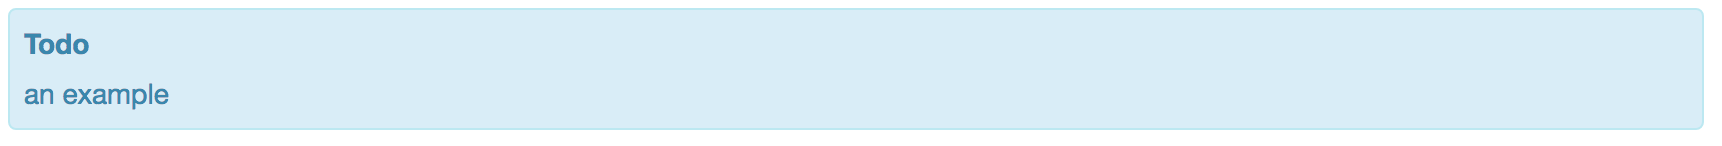
\includegraphics[width=\columnwidth]{images/todo.png}

\FILENAME

\section{Markdown}\label{S:markdown}

The content form this section originates from see:
\url{https://en.wikipedia.org/wiki/Markdown}.

Markdown is a simple markup language, however there is no precise
standard defined for it and implementations may have features not
supported by other implementations. Nevertheless, it provieds as imple
and easy way to quicly develop clean looking documents.

There are severla tools that make markdown attractive allowing to
write the text in one window while at the same time seeing the
rendered out put in another.

This includes

\begin{description}

\item[Macdown] An editor for mardown targeted on OSX

\end{description}

To convert the markdown to other formats with \verb|pandoc|

\begin{verbatim}
# Heading

## Sub-heading

### Another deeper heading
 
Paragraphs are separated
by a blank line.

Two spaces at the end of a line leave a  
line break.

Text attributes _italic_, *italic*, __bold__, **bold**, `monospace`.

Horizontal rule:

---

Bullet list:

  * apples
  * oranges
  * pears

Numbered list:

  1. apples
  2. oranges
  3. pears

A [link](http://example.com).

\end{verbatim}

\subsection{Tools}

\begin{description}
\item [Dilinger] \URL{https://dillinger.io/}. A HTML5 based cloud
  enabled editor. It allows to download the created Markdown.
\item[Macdown] \URL{https://macdown.uranusjr.com/} ``MacDown is an
  open source Markdown editor for macOS''
\end{description}

\subsection{Presentations in Markdown}

Please find some links on hwo to use markdown to create slides

\url{https://yhatt.github.io/marp/}

\url{http://slidify.org/}

\url{https://rmarkdown.rstudio.com/lesson-11.html}


GitPitch
\url{https://github.com/gitpitch/gitpitch/wiki/Slide-Markdown}
\FILENAME\

\section{Communicating Research in Other Ways}\label{communicating-research}

Naturally, writing papers is not the only way to communicate your
research with others. We find that today we see additional pathways
for cumminication includine blogs, twitter, facebook, e-mail, Web
pages, and electronic notebooks. Let us refisit some of them and
identify when they are helpful.

\subsection{Blogs}\label{blogs}

\begin{description}
\item[blog:]
noun, a regularly updated website or web page, typically one run by an
individual or small group, that is written in an informal or
conversational style.
\end{description}

Advantages:

\begin{itemize}

\item
  encourages spontaneous posts
\item
  encourages small short contributions
\item
  chronologically ordered
\item
  standard software exists to set up blogs
\item
  online services exists to set up blogs
\end{itemize}

Disadvantages:

\begin{itemize}

\item
  structuring data is difficult (some blog software support it)
\item
  not suitable for formal development of a paper
\item
  often lack of sophisticated track change features
\item
  no collaborative editing features
\end{itemize}

\subsection{Sphinx}\label{sphinx}

Sphinx (\url{http://www.sphinx-doc.org/}) is a tool that to create
integrated documentation from a markup language whlie.

Advantages:

\begin{itemize}

\item
  output formats: html, LaTeX, PDF, ePub
\item
  integrates well with directory structure
\item
  powerful markup language (reStructuredText)
\item
  can be hosted on github via github pages
\item
  can integare other renderers such as Markdown
\item
  automatic table of content, tebale of index
\item
  code documentation integration
\item
  search
\item
  written in python and using bash, so extensions and custom automation
  are possible
\end{itemize}

Disadvantage:

\begin{itemize}

\item
  requires compile step
\item
  When using markdown github can render individual page
\end{itemize}

Others:

\begin{itemize}

\item
  Read the Docs (\url{https://readthedocs.org/})
\item
  Doxygen (\url{http://www.stack.nl/~dimitri/doxygen/})
\item
  MkDocs (\url{http://www.mkdocs.org/})
\end{itemize}

\subsection{Notebooks}\label{notebooks}

\subsubsection{Jupyter}\label{jupyter}

The Jupyter Notebook (\url{http://jupyter.org/}) is an open-source web
application allowing users to create and share documents that contain
live code, equations, visualizations and explanatory text. Use cases
include data cleaning and transformation, numerical simulation,
statistical modeling, machine learning.

Advantages:

\begin{itemize}

\item
  Integrates with python
\item
  Recently other programming languages have been integrated
\item
  Allows experimenting with settings
\item
  Allows a form of literate programming while mixing documentation with
  code
\item
  automatically renders on github
\item
  comes with web service that allows hosting
\end{itemize}

Disadvantage:

\begin{itemize}

\item
  mostly encourages short documents
\item
  mark up language is limited
\item
  editing in ASCII is complex and Web editing is prefered
\end{itemize}

\subsubsection{Apache Zeppilin}\label{apache-zeppilin}

A Web-based notebook that enables data-driven, interactive data
analytics and collaborative documents with SQL, Scala and hadoop. It
integrates a web-based notebook with data ingestion, data exploration,
visualization, sharing and collaboration features to Hadoop and Spark.

Advantages:

\begin{itemize}

\item
  integration to various framework
\item
  Web framework
\item
  integration with spark, hadoop
\end{itemize}

Disadvantages:

\begin{itemize}

\item
  larger framework
\item
  must leverages existing deployments of spak, hadoop
\end{itemize}


\begin{comment}
\subsection{References}\label{references}

Collaboratories:

\begin{itemize}

\item
  Myers JD, TC Allison, SJ Bittner, BT Didier, M Frenklach, WH Green, YL
  Ho, J Hewson, WS Koegler, CS Lansing, D Leahy, M Lee, R McCoy, M
  Minkoff, S Nijsure, G von Laszewski, D Montoya, L Oluwole, CM
  Pancerella, R Pinzon, W Pitz, LA Rahn, B Ruscic, KL Schuchardt, EG
  Stephan, A Wagner, TL Windus, and C Yang. 2005. ``A Collaborative
  Informatics Infrastructure for Multi-scale Science.'' Cluster
  Computing 8(4):243-253.
\item
  Metadata in the Collaboratory for Multi-Scale Chemical Science Carmen
  Pancerella, John Hewson, Wendy Koegler, David Leahy, Michael Lee,
  Larry Rahn, Christine Yang, James D. Myers, Brett Didier, Renata
  McCoy, Karen Schuchardt, Eric Stephan, Theresa Windus, Kaizar Amin,
  Sandra Bittner, Carina Lansing, Michael Minkoff, Sandeep Nijsure,
  Gregor von Laszewski, Reinhardt Pinzon, Branko Ruscic, Al Wagner,
  Baoshan Wang, William Pitz, Yen-Ling Ho, David Montoya, Lili Xu,
  Thomas C. Allison, William H. Green, Jr., Michael Frenklach
  \url{http://dcpapers.dublincore.org/pubs/article/view/740/736}
\end{itemize}
\end{comment}

%%%%%%%%%%%%%%%%%%%%%%%%%%%%%%%%%%%%%%%%%%%%%%%%%%%%%%%%%%%%%%%%%%%%%%
%	FORMAT
%%%%%%%%%%%%%%%%%%%%%%%%%%%%%%%%%%%%%%%%%%%%%%%%%%%%%%%%%%%%%%%%%%%%%%

%
\chapterimage{water.png} % Chapter heading image

\chapter{Book Format}

\FILENAME

This document is prepared using a special enhanced \LaTeX book format to allow
easy integration for section and index references, as well as
citations and other straight forward enhancements that makes it easy
for students to obtain a document with much of the Lecture material
included. We provide some examples so that if you like to contribute
you can do so easily and can use the correct way of doing so.


\section{Paragraphs of Text}\index{\LaTeX!Book!Paragraphs of Text}

\lipsum[1] % Dummy text

%------------------------------------------------

\section{Citation}\index{\LaTeX!Book!Citation}

\begin{tcblisting}{colback=blue!5!white,colframe=gray!50!blue,listing side text,
  title=Numbered List,fonttitle=\bfseries}
This statement requires citation \cite{article_key}; 
this one is more specific \cite[162]{book_key}.
\end{tcblisting}

%------------------------------------------------

\section{Lists}\index{\LaTeX!Book!Lists}

Lists are useful to present information in a concise and/or ordered way\footnote{Footnote example...}.

\subsection{Numbered List}\index{\LaTeX!Book!Lists!Numbered List}

\begin{tcblisting}{colback=blue!5!white,colframe=gray!50!blue,listing side text,
  title=Numbered List,fonttitle=\bfseries}
\begin{enumerate}
\item The first item
\item The second item
\item The third item
\end{enumerate}
\end{tcblisting}

\subsection{Bullet Points}\index{\LaTeX!Book!Lists!Bullet Points}

\begin{tcblisting}{colback=blue!5!white,colframe=gray!50!blue,listing side text,
  title=Bullet Points,fonttitle=\bfseries}
\begin{itemize}
\item The first item
\item The second item
\item The third item
\end{itemize}
\end{tcblisting}

\subsection{Descriptions and Definitions}\index{\LaTeX!Book!Lists!Descriptions and Definitions}

\begin{tcblisting}{colback=blue!5!white,colframe=gray!50!blue,listing side text,
  title=Enumerations,fonttitle=\bfseries}
\begin{description}
\item[Name] Description
\item[Word] Definition
\item[Comment] Elaboration
\end{description}
\end{tcblisting}

%-------------------------------------------------------------------------------
%	CHAPTER 2
%-------------------------------------------------------------------------------


\section{Theorems}\index{\LaTeX!Book!Theorems}

This is an example of theorems.

\subsection{Several equations}\index{\LaTeX!Book!Theorems!Several Equations}
This is a theorem consisting of several equations.

\begin{lstlisting}
\begin{theorem}[Name of the theorem]
In $E=\mathbb{R}^n$ all norms are equivalent. It has the properties:
\begin{align}
& \big| ||\mathbf{x}|| - ||\mathbf{y}|| \big|\leq || \mathbf{x}- \mathbf{y}||\\
&  ||\sum_{i=1}^n\mathbf{x}_i||\leq \sum_{i=1}^n||\mathbf{x}_i||\quad\text{where $n$ is a finite integer}
\end{align}
\end{theorem}
\end{lstlisting}

\begin{theorem}[Name of the theorem]
In $E=\mathbb{R}^n$ all norms are equivalent. It has the properties:
\begin{align}
& \big| ||\mathbf{x}|| - ||\mathbf{y}|| \big|\leq || \mathbf{x}- \mathbf{y}||\\
&  ||\sum_{i=1}^n\mathbf{x}_i||\leq \sum_{i=1}^n||\mathbf{x}_i||\quad\text{where $n$ is a finite integer}
\end{align}
\end{theorem}

\subsection{Single Line}\index{\LaTeX!Book!Theorems!Single Line}
This is a theorem consisting of just one line.

\begin{verbatim}
\begin{theorem}
A set $\mathcal{D}(G)$ in dense in $L^2(G)$, $|\cdot|_0$. 
\end{theorem}
\end{verbatim}

\begin{theorem}
A set $\mathcal{D}(G)$ in dense in $L^2(G)$, $|\cdot|_0$. 
\end{theorem}

%------------------------------------------------

\section{Definitions}\index{\LaTeX!Book!Definitions}

This is an example of a definition. A definition could be mathematical or it could define a concept.

\begin{definition}[Definition name]
Given a vector space $E$, a norm on $E$ is an application, denoted $||\cdot||$, $E$ in $\mathbb{R}^+=[0,+\infty[$ such that:
\begin{align}
& ||\mathbf{x}||=0\ \Rightarrow\ \mathbf{x}=\mathbf{0}\\
& ||\lambda \mathbf{x}||=|\lambda|\cdot ||\mathbf{x}||\\
& ||\mathbf{x}+\mathbf{y}||\leq ||\mathbf{x}||+||\mathbf{y}||
\end{align}
\end{definition}

%------------------------------------------------

\section{Notations}\index{\LaTeX!Book!Notations}

\begin{tcblisting}{colback=blue!5!white,colframe=gray!50!blue,listing side text,  title=Exercise,fonttitle=\bfseries}
\begin{notation}
Given an open subset $G$ of $\mathbb{R}^n$, the set of functions $\varphi$ are:
\begin{enumerate}
\item Bounded support $G$;
\item Infinitely differentiable;
\end{enumerate}
a vector space is denoted by $\mathcal{D}(G)$. 
\end{notation}
\end{tcblisting}

%------------------------------------------------

\section{Remarks}\index{\LaTeX!Book!Remarks}

This is an example of a remark.

\begin{tcblisting}{colback=blue!5!white,colframe=gray!50!blue,listing side text,  title=Exercise,fonttitle=\bfseries}
\begin{remark}
The concepts presented here are now in conventional employment in mathematics. Vector spaces are taken over the field $\mathbb{K}=\mathbb{R}$, however, established properties are easily extended to $\mathbb{K}=\mathbb{C}$.
\end{remark}
\end{tcblisting}

%------------------------------------------------

\section{Corollaries}\index{\LaTeX!Book!Corollaries}

This is an example of a corollary.
\begin{tcblisting}{colback=blue!5!white,colframe=gray!50!blue,listing
    side text,  title=Exercise,fonttitle=\bfseries}
\begin{corollary}[Corollary name]
The concepts presented here are now in conventional employment in mathematics. Vector spaces are taken over the field $\mathbb{K}=\mathbb{R}$, however, established properties are easily extended to $\mathbb{K}=\mathbb{C}$.
\end{corollary}
\end{tcblisting}
%------------------------------------------------

\section{Propositions}\index{\LaTeX!Book!Propositions}

These are examples of propositions.

\subsection{Several equations}\index{\LaTeX!Book!Propositions!Several Equations}


\begin{proposition}[Proposition name]
It has the properties:
\begin{align}
& \big| ||\mathbf{x}|| - ||\mathbf{y}|| \big|\leq || \mathbf{x}- \mathbf{y}||\\
&  ||\sum_{i=1}^n\mathbf{x}_i||\leq \sum_{i=1}^n||\mathbf{x}_i||\quad\text{where $n$ is a finite integer}
\end{align}
\end{proposition}

\subsection{Single Line}\index{\LaTeX!Book!Propositions!Single Line}

\begin{proposition} 
Let $f,g\in L^2(G)$; if $\forall \varphi\in\mathcal{D}(G)$, $(f,\varphi)_0=(g,\varphi)_0$ then $f = g$. 
\end{proposition}

%------------------------------------------------

\section{Examples}\index{\LaTeX!Book!Examples}

This is an example of examples.

\subsection{Equation and Text}\index{\LaTeX!Book!Examples!Equation and Text}

\begin{example}
Let $G=\{x\in\mathbb{R}^2:|x|<3\}$ and denoted by: $x^0=(1,1)$; consider the function:
\begin{equation}
f(x)=\left\{\begin{aligned} & \mathrm{e}^{|x|} & & \text{si $|x-x^0|\leq 1/2$}\\
& 0 & & \text{si $|x-x^0|> 1/2$}\end{aligned}\right.
\end{equation}
The function $f$ has bounded support, we can take $A=\{x\in\mathbb{R}^2:|x-x^0|\leq 1/2+\epsilon\}$ for all $\epsilon\in\intoo{0}{5/2-\sqrt{2}}$.
\end{example}

\subsection{Paragraph of Text}\index{\LaTeX!Book!Examples!Paragraph of Text}

\begin{tcblisting}{colback=blue!5!white,colframe=gray!50!blue,listing side text,  title=Example,fonttitle=\bfseries}
\begin{example}[Example name]
\lipsum[1]
\end{example}
\end{tcblisting}

%------------------------------------------------

\section{Exercises}\index{\LaTeX!Book!Exercises}

This is an example of an exercise.

\begin{tcblisting}{colback=blue!5!white,colframe=gray!50!blue,listing side text,  title=Exercise,fonttitle=\bfseries}
\begin{exercise}
This is a good place to ask a question to test learning progress or further cement ideas into students' minds.
\end{exercise}
\end{tcblisting}

%------------------------------------------------

\section{Problems}\index{\LaTeX!Book!Problems}

\begin{tcblisting}{colback=blue!5!white,colframe=gray!50!blue,listing side text,  title=Exercise,fonttitle=\bfseries}
\begin{problem}
What is the average airspeed velocity of an unladen swallow?
\end{problem}
\end{tcblisting}

%------------------------------------------------

\section{Vocabulary}\index{\LaTeX!Book!Vocabulary}

Define a word to improve a students' vocabulary.

\begin{tcblisting}{colback=blue!5!white,colframe=gray!50!blue,listing side text,  title=Exercise,fonttitle=\bfseries}
\begin{vocabulary}[Word]
Definition of word.
\end{vocabulary}
\end{tcblisting}

\section{Tables}\index{\LaTeX!Book!Table}

\begin{table}[h]
\centering
\begin{tabular}{l l l}
\toprule
\textbf{Treatments} & \textbf{Response 1} & \textbf{Response 2}\\
\midrule
Treatment 1 & 0.0003262 & 0.562 \\
Treatment 2 & 0.0015681 & 0.910 \\
Treatment 3 & 0.0009271 & 0.296 \\
\bottomrule
\end{tabular}
\caption{Table caption}
\end{table}

%------------------------------------------------

\section{Figures}\index{\LaTeX!Book!Figure}

\begin{figure}[h]
\centering
\includegraphics[scale=0.5]{placeholder}
\caption{Figure caption}
\end{figure}

\subsection{Colored Boxes}
\index{\LaTeX!Book!Boxes}
\index{\LaTeX!Book!NOTE}
\index{\LaTeX!Book!WARNING}
\index{\LaTeX!Book!IU}

The package \verb|tcolorbox| provides sophisticated support to include
color boxes. Together with the new environment we can create nice add
ons to for example include notes.

\URL{http://osl.ugr.es/CTAN/macros/latex/contrib/tcolorbox/tcolorbox.pdf}

We have provided in this document notes as follows


\begin{tcblisting}{colback=blue!5!white,colframe=gray!50!blue,listing side text,  title=Note,fonttitle=\bfseries}
\begin{NOTE}
This is a note
\end{NOTE}
\end{tcblisting}

\begin{tcblisting}{colback=blue!5!white,colframe=gray!50!blue,listing side text,  title=Warning,fonttitle=\bfseries}
\begin{WARNING}
This is a note
\end{WARNING}
\end{tcblisting}

\begin{tcblisting}{colback=blue!5!white,colframe=gray!50!blue,listing side text,  title=Warning,fonttitle=\bfseries}
\begin{IU}
This is a note
\end{IU}
\end{tcblisting}

\subsection{Section References}

Section references with the Where command are used to refer to a
section by label, but be presented with the section number, the title,
and the page number. It can be augmented with a text, such as in which
week the section is best to be studied. This is useful for creating a
customized Syllabus

\begin{tcblisting}{colback=blue!5!white,colframe=gray!50!blue,
    listing side text, title=Warning,fonttitle=\bfseries}
\WHERE{\YES}{C:linux}{Week 2}
\end{tcblisting}

\begin{tcblisting}{colback=blue!5!white,colframe=gray!50!blue,
    listing side text, title=Warning,fonttitle=\bfseries}
\WHERE{\NO}{C:linux}{Week 2}
\end{tcblisting}

The checkmark indicate if the lecture has been released for the
ongoing semester.



 
%----------------------------------------------------------------------------------------
%	LINUX
%----------------------------------------------------------------------------------------


\part{Development Tools and Services}

% chktex-file 44
% chktex-file 8
% chktex-file 1

\chapter{Linux}
\label{C:linux}
\index{Linux}

\FILENAME\

\section{History}

LINUX is a reimplementation by the community of UNIX which was
developed in 1969 by Ken Thompson and Dennis Ritchie of Bell
Laboratories and rewritten in C. An important part of UNIX is what is
called the \textit{kernel} which allows the software to talk to
the hardware and utilize it. 

In 1991 Linus Trovalds started developing a Linux Kernel that was
initially targeted for PC's. This made it possible to run it on
Laptops and was later on further developed by making it a full
Operating system replacement for UNIX. 

\section{Shell}
\label{c:linux-commands}
\index{Shell}
\index{Terminal}

One of the most important features for us will be to access the
computer with the help of a \textit{shell}. The shell is typically run in
what is called a terminal and allows interaction to the computer with
commandline programs. 

There are many good tutorials out there that explain why one needs a
linux shell and not just a GUI. Randomly we picked the first one that
came up with a google query. This is not an endorsement for the material
we point to, but could be a worth while read for someone that has no
experience in Shell programming:

\URL{http://linuxcommand.org/lc3_learning_the_shell.php}

Certainly you are welcome to use other resources that may suite you
best. We will however summarize in table form a number of useful
commands that you may als find even as a RefCard.

\URL{http://www.cheat-sheets.org/\#Linux}

We provide in Table~\ref{T:shell-commands} a number of useful commands
that you want to explore. For more information simply type man and the
name of the command.


\begin{center}
\begin{longtable}{|p{4cm}|p{8cm}|}
\caption{Common commands}\label{T:shell-commands}\\

\hline
\multicolumn{1}{|p{4cm}|}{\textbf{Example}} & \multicolumn{1}{p{8cm}|}{\textbf{Description}} \\ 
\hline 
\endfirsthead

\multicolumn{2}{p{12cm}}%
{{\bfseries \tablename\ \thetable{} -- continued from previous page}} \\
\hline 
\hline \multicolumn{1}{|p{4cm}|}{\textbf{Example}} & \multicolumn{1}{p{8cm}|}{\textbf{Description}} \\ 
\hline 
\endhead

\hline 
\multicolumn{2}{|r|}{{Continued on next page}} \\
\hline
\endfoot

%\hline 
\hline
\endlastfoot

  \multicolumn{2}{|l|}{\cellcolor{blue!15} Help Commands}\\
  \hline
  man \emph{command} & manual page for the \emph{command} \\
  apropos \textit{text} & list all commands that have text in it\\
  & \\

  \hline
  \multicolumn{2}{|l|}{\cellcolor{blue!15} File Commands}\\
  \hline
  ls & Directory listing\\
  ls -lisa & list details \\
  tree & list the directories in graphical form \\
  cd \emph{dirname} & Change directory to \emph{dirname} \\
  mkdir \emph{dirname} & create the directory \\
  rmdir \emph{dirname} & delete the directory \\
  pwd & print working directory \\
  rm \emph{file} & remove the file \\
  cp \emph{a} \emph{b} & copy file \emph{a} to \emph{b} \\
  mv \emph{a} \emph{b} & move/rename file \emph{a} to \emph{b}\\
  cat \emph{a} & print content of file\emph{a}\\
  cat -n &  (assignment) \\
  less \emph{a} & print paged content of file \emph{a}\\
  head -5 \emph{a} & Display first 5 lines of file \emph{a}\\
  tail -5 \emph{a} & Display last 5 lines of file \emph{a}\\
  \verb|du -hs .| & show in human readable form the space used by the current
             directory\\
  \verb|df -h| & show the details of the disk file system \\
  wc \textit{filename}&  counts the word in a file \\
  sort \textit{filename} &  sorts the file \\
  uniq \textit{filename} &  displays only uniq entries in the file \\
  tar -xvf \textit{dir} &  tars up a compressed version of the directory \\
  rsync &  (assignment) \\
  gzip &  (assignment) \\
  gunzip &  (assignment) \\
  bzip2 &  (assignment) \\
  bunzip2 &  (assignment) \\
  clear & \\
  touch & \\
  who & \\
  whoami & \\
  echo & \\
  data & \\
  logout & \\
  exit & \\
  kill & \\
  ps & \\
  sleep & \\
  uptime & \\
  time & \\
  date & \\
  find & \\
  diff & \\
  hostname & \\
  which & \\
  tail & \\
  head & \\
  top & \\
  locate \textit{filename} & \\
  grep & \\
  chmod ug+rw \textit{filename} & \\
  chown & \\
  history & \\
  sudo & \\
  su & \\
  uname & \\
  set -o emacs & \\
  & \\
  
  %\hline
  %\multicolumn{2}{|l|}{\cellcolor{blue!15} Search Commands}\\
  %\hline
  chmod go-rwx \textit{file} & changes the permission of the file \\
  chown \textit{username} \textit{file} & changes the ownership of the file \\
  chgrp \textit{group} \textit{file} & changes the group of a file\\
  & \\

  \hline
  \multicolumn{2}{|l|}{\cellcolor{blue!15} Search Commands}\\
  \hline
  \verb|fgrep "text" filename| &  searches the text in the given file \\
  \verb|grep -R "xyz" .| & recursively searches for xyz in all files \\
  \verb|find . -name "*.py"| &  find all files with \verb|.py| at the end \\
  & \\

  %\hline
  %\multicolumn{2}{|l|}{\cellcolor{blue!15} Process Commands}\\
  %\hline
  ps & list the running processes \\
  kill -9 1234 & kill the process with the id 1234 \\
  at &  (assignment) \\
  cron &  (assignment) \\
  crontab &  (assignment) \\
  & \\

  \hline
  \multicolumn{2}{|l|}{\cellcolor{blue!15} Device Commands}\\
  \hline
  mount /dev/cdrom /mnt/cdrom & mount a filesystem from a cd rom to /mnt/cdrom\\
  & \\

  \hline
  \multicolumn{2}{|l|}{\cellcolor{blue!15} System Commands}\\
  \hline
  users &  (assignment) \\
  who &  (assignment) \\
  whoami &  (assignment) \\
  dmesg &  (assignment) \\
  last &  (assignment) \\
  free -tm &  (assignment) \\
  uname &  (assignment) \\
  date &  prints the current date and time \\
  time \textit{command} &  prints the sys, real and user time \\
  shutdown -h ``shut down'' & (assignment) \\
  & \\

  \hline
  \multicolumn{2}{|l|}{\cellcolor{blue!15} Networking Commands}\\
  \hline
  ping &  (assignment) \\
  netstat &  (assignment) \\
  hostname &  (assignment) \\
  traceroute &  (assignment) \\
  ifconfig &  (assignment) \\
  & \\

  \hline
  \multicolumn{2}{|l|}{\cellcolor{blue!15} Internet Commands}\\
  \hline
  host &  (assignment) \\
  whois &  (assignment) \\
  dig &  (assignment) \\
  wget &  (assignment) \\
  curl &  (assignment) \\
  & \\

  \hline
  \multicolumn{2}{|l|}{\cellcolor{blue!15} Remote Access Commands}\\
  \hline
  ssh &  (assignment) \\
  scp &  (assignment) \\
  sftp &  (assignment) \\
  & \\


\end{longtable}
\end{center}

\section{Multi-command execution}

One of the important features is that one can execute multiple
commands in the shell.

To execute command 2 once command 1 has finished use

\begin{verbatim}
command1; command2
\end{verbatim}

To execute command 2 as soon as command 1 forwards output to stdout use

\begin{verbatim}
command1; command2
\end{verbatim}

To execute command 1 in the background use

\begin{verbatim}
command1 &
\end{verbatim}



\section{Keyboard Shortcuts}\label{keyboard-shortcuts}

These shortcuts will come in handy. Note that many overlap with emacs
short cuts.

\begin{tabular}{ll}
Keys     & Description  \\
\hline
Up Arrow & Show the previous command\\
Ctrl + z & Stops the current command  \\
         & Resume with fg in the foreground \\
         & Resume with bg in the background \\
Ctrl + c & Halts the current command\\
Ctrl + l & Clear the screen\\
Ctrl + a & Return to the start of the line\\
Ctrl + e & Go to the end of the line\\
Ctrl + k & Cut everything after the cursor to a special clipboard\\
Ctrl + y & Paste from the special clipboard \\
Ctrl + d & Logout of current session, similar to exit \\
\end{tabular}

\section{bashrc and bash\_profile}
\index{.bashrc}

Usage of a particular command and all the attributes associated with it,
use `man' command. Avoid using \verb|rm -r| command to delete files
recursively. A good way to avoid accidental deletion is to include the
following in your \verb|.bash_profile| file:

\begin{verbatim}
alias e=open_emacs
alias rm='rm -i'
alias mv='mv -i' 
alias h='history'
\end{verbatim}

More Information

\url{https://cloudmesh.github.io/classes/lesson/linux/refcards.html}

\section{Makefile}
\label{s:makefile}
\index{Makefile}

Makefiles allow developers to coordinate the execution of code
compilations. This not only includes C or C++ code, but any
translation from source to a final format. For us this could include
the creation of PDF files from latex sources, creation of docker
images, and the creation of cloud services and their deployment
through simple workflows represented in makefiles, or the coordination
of execution targets.

As makefiles include a simple syntax allowing structural dependencies
they can easily adapted to fulfill simple activities to be executed in
repeated fashion by developers.

An example of how to use Makefiles for docker is provided at
\url{http://jmkhael.io/makefiles-for-your-dockerfiles/}.

An example on how to use Makefiles for \LaTeX~is provided at
\url{https://github.com/cloudmesh/book/blob/master/Makefile}.

Makefiles include a number of rules that are defined by a target
name. Let us define a target called hello that prints out the string
``Hello World''.

\begin{lstlisting} 
hello:
    @echo "Hello World"
\end{lstlisting} 

Important to remember is that the commands after a target are not
indented just by spaces, but actually by a single TAB
character. Editors such as emacs will be ideal to edit such Makefiles,
while allowing syntax highlighting and easy manipulation of
TABs. Naturally other editros will do that also. Please chose your
editor of choice. One of the best features of targets is that they can
depend on other targets. Thus, iw we define

\begin{lstlisting} 
hallo: hello
    @echo "Hallo World"
\end{lstlisting} 

our makefile will first execute hello and than all commands in hallo.
As you can see this can be very useful for defining simple
dependencies. 

In addition we can define variables in a makefile such as 

\begin{lstlisting} 
HELLO="Hello World"

hello: 
    @echo $(HELLO)
\end{lstlisting} 
%$

and can use them in our text with \$ invocations.

Moreover, in sophisticated Makefiles, we could even make the targets
dependent on files and a target rouls could be defined that only
compiles those files that have changed since our last invokation of
the Makefile, saving potentially a lot of time. However, for our work
here we just use the most elementary makefiles.

For more information we recommend you to find out about it on the internet.
A convenient refrence card sis available at~\url{http://www.cs.jhu.edu/~joanne/unixRC.pdf}.


\subsubsection{Makefiles on Windows}
\index{Makefile!Windows}

Makefiles can easily be accessed also on windows while installing
gitbash. Please reer to the internet or search in this handbook for
more information about gitbash.



\section{Exercises}

\begin{exercise}
\label{E:Linux.1}
Familiarize yourself with the commands
\end{exercise}

\begin{exercise}
\label{E:Linux.2}
Find more commands that you find useful and add them to this page.
\end{exercise}

\begin{exercise}
\label{E:Linux.3}
Use the sort command to sort all lines of a file while removing
duplicates.
\end{exercise}

\begin{exercise}
\label{E:Linux.4} In Table~\ref{T:shell-commands} you will find a number
  of commands with (assignment). Develop descriptions that you will
  contribute and add to the manual with a pull request. Work in a team
  so that only one pull request is issued. Do not only provide the
  description, but also a real example as showcased within the table.
\end{exercise}

\begin{exercise}
\label{E:Linux.4} Should there be other commands listed in the table. If
  so which? Create a pull request for them. 
\end{exercise}


\


\chapter{Github}
\label{C:github}

\FILENAME

In some classes the material may be openly shared in code
repositories. This includes class material, papers and project.
Hence, we need some mechanism to share content with a large number of
students. For this reason we use \URL{github.com}.

First, we like to introduce you to git and github.com (Section
\ref{s:github}).  Next, we provide you with the basic commands to
interact with git from the commandline (Section
\ref{s:git-commands}). Than we will introduce you how you can
contribute to this set of documentations with pull requests.

\section{Obverview}\label{s:github}

Github is a code repository that allows the development of code and
documents with many contributors in a distributed fashion. There are
many good tutorials about github.  Some of them can be found on the
github Web page. An interactive tutorial is for example available at

\URL{https://try.github.io/}

However, although these tutorials are helpful in many cases they do
not address some cases. For example, you have already a repository set
up by yoru organization and you do not have to completely initialize
it. Thus do not just replicate the commands in the tutorial, or the
once we present here before not evaluating their consequences. In
general make sure you verify if the command does what you expect {\bf
  before} you execute it.

A more extensive list of tutorials can be found at

\URL{https://help.github.com/articles/what-are-other-good-resources-for-learning-git-and-github}

The github foundation has a number of excellent videos about git. If you
are unfamiliar with git and you like to watch videos in addition to
reading the documentation we recommend these videos

\URL{https://www.youtube.com/user/GitHubGuides/videos}

Next, we introduce some important concepts used in github.

\section{Upload Key}\label{upload-key}

Before you can work with a repository in an easy fashion you need to
upload a public key in order to access your repository. Naturally, you
need to generate a key first which is explained in 

\TODO{lessons-ssh-generate-key}

before you upload one. Copy the contents of your
\verb|.ssh/id_rsa.pub| file and add them to
\href{https://github.com/settings/keys}{your github keys}.

More information on this topic can be found on the
\href{https://help.github.com/articles/adding-a-new-ssh-key-to-your-github-account/}{github
  Web page}.

\section{Fork}\label{fork}

Forking is the first step to contributing to projects on GitHub. Forking
allows you to copy a repository and work on it under your own account.
Next, creating a branch, making some changes, and offering a pull
request to the original repository, rounds out your contribution to the
open source project.

\video{Git}{1:41}{Fork}{https://www.youtube.com/watch?v=5oJHRbqEofs}

\section{Rebase}\label{rebase}

When you start editing your project, you diverge from the original
version. During your developing, the original version may be updated, or
other developers may have some of their branches implementing good
features that you would like to include in your current work. That is
when {\em Rebase} becomes useful. When you {\em Rebase} to certain points, could
be a newer Master or other custom branch, consider you graft all your
on-going work right to that point.

Rebase may fail, because some times it is impossible to achieve what we
just described as conflicts may exist. For example, you and the to-be-rebased copy
both edited some common text section. Once this happens, human
intervention needs to take place to resolve the conflict.

\video{Git}{4:20}{Rebase}{https://www.youtube.com/watch?v=SxzjZtJwOgo}

\section{Remote}\label{remote}

Collaborating with others involves managing the remote repositories
and pushing and pulling data to and from them when you need to share
work. Managing remote repositories includes knowing how to add remote
repositories, remove remotes that are no longer valid, manage various
remote branches and define them as being tracked or not, and more.

Though out this semester, you will typically work on two {\em remote} repos.
One is the office class repo, and another is the repo you forked from
the class repo. The class repo is used as the centralized, authority and
final version of all student submissions. The repo under your own Github
account is for your personal storage. To show progress on a weekly
basis you need to commit your changes on a weekly basis. However make
sure that things in the master branch are working. If not, just use
another branch to conduct your changes and merge at a later
time. we like you to call your development branch {\ dev}.

\URL{https://git-scm.com/book/en/v2/Git-Basics-Working-with-Remotes}

\section{Pull Request}\label{pull-request}

Pull requests are a means of starting a conversation about a proposed
change back into a project. We will be taking a look at the strength of
conversation, integration options for fuller information about a change,
and cleanup strategy for when a pull request is finished.

\video{Git}{4:26}{Pull Request}{https://www.youtube.com/watch?v=d5wpJ5VimSU}

\section{Branch}\label{branch}

Branches are an excellent way to not only work safely on features or
experiments, but they are also the key element in creating Pull Requests
on GitHub. Lets take a look at why we want branches, how to create and
delete branches, and how to switch branches in this episode.

\video{Git}{2:25}{Branch}{https://www.youtube.com/watch?v=H5GJfcp3p4Q}

\section{Checkout}\label{checkout}

Change where and what you are working on with the checkout command.
Whether we are switching branches, wanting to look at the working tree at
a specific commit in history, or discarding edits we want to throw away,
all of these can be done with the checkout command.

\video{Git}{3:11}{Checkout}{https://www.youtube.com/watch?v=HwrPhOp6-aM}


\section{Merge}\label{merge}

Once you know branches, merging that work into master is the natural
next step. Find out how to merge branches, identify and clean up merge
conflicts or avoid conflicts until a later date. Lastly, we will look at
combining the merged feature branch into a single commit and cleaning up
your feature branch after merges.

\video{Git}{3:11}{Merge}{https://www.youtube.com/watch?v=yyLiplDQtf0}

\section{GUI}\label{gui}

Using Graphical User Interfaces can supplement your use of the command
line to get the best of both worlds. GitHub for Windows and GitHub for
Mac allow for switching to command line, ease of grabbing repositories
from GitHub, and participating in a particular pull request. We will also
see the auto-updating functionality helps us stay up to date with stable
versions of Git on the command line.

\video{Git}{3:47}{GUI}{https://www.youtube.com/watch?v=BMYOs5jflGE}

There are many other git GUI tools available that directly integrate into your
operating system finders, windows, \ldots{}, or PyCharm. It is up to you
to identify such tools and see if they are useful for you. Most of the
people we work with us git from the command line, even if they use
PyCharm, eclipse, or other tools that have build in git support. You can
identify a tool that works best for you.

\section{Windows}\label{windows}

This is a quick tour of GitHub for Windows. It offers GitHub newcomers a
brief overview of what this feature-loaded version control tool and an
equally powerful web application can do for developers, designers, and
managers using Windows in both the open source and commercial software
worlds. More: \url{http://windows.github.com}

\video{Git}{1:25}{Windows}{https://www.youtube.com/watch?v=YBbkvCrfDSo}


\section{Git from the Commandline}\label{s:git-commands}

Although github.com provides a powerful GUI and other GUI tools are
available to interface with github.com, the use of git from the
commandline can often be faster and in many cases may be simpler. 

Git commandline tools can be easily installed on a variety of
operating systems including Linux, OSX, and Windows. Many great
tutorials exist that will allow you to complete this task easily. We
found the following two tutorials sufficient to get the task
accomplished:

\URL{https://git-scm.com/book/en/v2/Getting-Started-Installing-Git}

\URL{https://www.atlassian.com/git/tutorials/install-git}

Although the later is provided by an alternate repository to
github. The installation instructions are very nice and are not
impacted by it. Once you have installed git you need to configure it.

\section{Configuration}\label{config}

Once you installed Git, you can need to configure it properly.  This
includes setting up your username, email address, line endings, and
color, along with the settings' associated configuration scopes.

\video{Git}{2:47}{Configuration}{https://www.youtube.com/watch?v=ZChtKFLiaNw}

It is important that make sure that use the \verb|git config| command
to initialize git for the first time on each new computer system or
virtual machine you use. This will ensure that you use on all
resources the same name and e-mail so that git history and log will
show consistently your checkins across all devices and computers you
use.  If you do not do this, your checkins in git do not show up in a
consistent fashion as a single user. Thus on each computer execute the
following commands:

\begin{verbatim}
$ git config --global user.name "Albert Zweistein"
$ git config --global user.email albert.zweistein@gmail.com
\end{verbatim}

where you replace the information with the information related to you.
You can set the editor to emacs with:

\begin{verbatim}
$ git config --global core.editor emacs
\end{verbatim}

Naturally if you happen to want to use other editors you can configure
them by specifying the command that starts them up. You will also need
to decide if you want to push branches individually or all branches at
the same time. It will be up to you to make what whill work for you
best. We found that the following seems to work best:

\begin{verbatim}
git config --global push.default matching
\end{verbatim}

More information about a first time setup is documented at:

\begin{verbatim}
* http://git-scm.com/book/en/Getting-Started-First-Time-Git-Setup
\end{verbatim}

To check your setup you can say:

\begin{verbatim}
$ git config --list
\end{verbatim}

One problem we observed is that students often simply copy and paste
instructions, but do not read carefully the error that is reported
back and do not fix it. Overlooking the proper set of the push.default
is often overlooked. Thus we remind you: {\bf Please read the
  information on the screen when you set up}.

\section{Upload your public key}\label{upload-your-public-key}

Please upload your public key to the repository as documented in
github, while going to your account and find it in settings. There you
will find a panel SSH key that you can click on which brings you to
the window allowing you to add a new key. If you have difficulties
with this find a video from the github foundation that explains this.

\section{Working with a directory that was provided for you}

In case your course provided you with a github directory, starting and
working in it is going to be real simple. If you are the only student
working on this you still need to make sure that papers or programs
you manage in the repository work and do not interfere with scripts
that instructors may use to check your assignments. Thus it is god to
still create a branch, work in the branch and than merge the branch
into the master once you verified things work. After you merged you
can push the content to the github repository.

Tip: Please use only \textbf{lowercase} characters in the directory
names and no special characters such as @ ; / \_ and spaces. In general
we recommend that you avoid using directoru names with capital letters
spaces and \_ in them. This will simplify your documentation efforts and
make the URLs from git more readable. Also while on some OS's the
directories {\em MyDirectory} is different from {\em mydirectory} on OSX
it is considered the same and thus renaming from capital to lower case
can not be done without first renaming it to another directory. 


Your homework for submission should be organized according to folders in
your clone repository. To submit a particular assignment, you must first
add it using:

\begin{verbatim}
git add <name of the file you are adding>
\end{verbatim}

Afterwards, commit it using:

\begin{verbatim}
git commit -m "message describing your submission"
\end{verbatim}

Then push it to your remote repository using:

\begin{verbatim}
git push
\end{verbatim}

If you want to modify your submission, you only need to:

\begin{verbatim}
git commit -m "message relating to updated file"
\end{verbatim}

afterwards:

\begin{verbatim}
git push
\end{verbatim}

If you lose any documents locally, you can retrieve them from your
remote repository using:

\begin{verbatim}
git pull
\end{verbatim}

\section{README.yml and notebook.md}

In case you take classes e516 and e616 with us you will have to create
a README.yaml and notebook.md file in the top most directory of your
repository. It serves the purpose of identifying your submission for
homework and information about yourself.

It is important to follow the format precisely. As it is yaml it is an
easy homework to write a 4 line python script that validates if the
README.yaml file is valid. In addition you can use programs such as
\verb|yamllint| which is documented at 

\URL{https://yamllint.readthedocs.io/en/latest/}

This file is used to integrate your assignments into a proceedings. An
example is provided at 

\URL{https://github.com/bigdata-i523/sample-hid000/blob/master/README.yml}

Any derivation from this format will not allow us to see your homework
as our automated scripts will use the README.yml to detect
them. Make sure the file does not
contain ay TABs.  Please also mind that all filenames of all homework
and the main directory must be \textbf{lowercase} and do not include
spaces. This will simplify your task of managing the files across
different operating systems.

In case you work in a team, on a submission, the document will only be
submitted in the author and hid that is listed first. All other
readmes, will have for that particular artifact a
\verb|duplicate: yes| entry to indicate that this submission is
managed elswhere. The team will be responsible to manage their own
pull requests, but if the team desires we can grant access for all
memebers to a repository by a user. Please be aware that you must make
sure you coordinate with your team.

We will not accept submission of homework as pdf documents or tar
files. All assignments must be submitted as code and the reports in
native latex and in github. We have a script that will automatically
create the PDF and include it in a proceedings. There is no exception
from this rule and all reports not compilable will be returned without
review and if not submitted within the deadline receive a panelty.

Please check with your instructor on the format of the README.yaml
file as it could be different for your class. 

\section{Contributing to the Document}

\TODO{This section has to be redone as we use class specific clones
  and not the master}


\subsection{Clone}

\begin{verbatim}
$ git remote add upstream https://github.com/cloudmesh/book
\end{verbatim}


\subsection{Merge}

As we are allowing contribution by the community, they are best managed
through a merge with our upstream repository so you can update to the
newest status before you issue a pul request.

Make sure you have upstream repo defined:

\begin{verbatim}
$ git remote add upstream https://github.com/cloudmesh/book
\end{verbatim}

Now Get latest from upstream:

\begin{verbatim}
$ git rebase upstream/master
\end{verbatim}

In this step, the conflicting file shows up (in my case it was
refs.bib):

\begin{verbatim}
$ git status
\end{verbatim}

should show the name of the conflicting file:

\begin{verbatim}
$ git diff <file name>
\end{verbatim}

should show the actual differences. May be in some cases, It is easy to
simply take latest version from upstream and reapply your changes.

So you can decide to checkout one version earlier of the specific file.
At this stage, the re-base should be complete. So, you need to commit
and push the changes to your fork:

\begin{verbatim}
$ git commit
$ git rebase origin/master
$ git push
\end{verbatim}

Then reapply your changes to refs.bib - simply use the backedup version
and use the editor to redo the changes.

At this stage, only refs.bib is changed:

\begin{verbatim}
$ git status
\end{verbatim}

should show the changes only in refs.bib. Commit this change using:

\begin{verbatim}
$ git commit -a -m "new:usr: <message>"
\end{verbatim}

And finally push the last commited change:

\begin{verbatim}
$ git push
\end{verbatim}

The changes in the file to resolve merge conflict automatically goes to
the original pull request and the pull request can be merged
automatically.

You still have to issue the pull request from the Github Web page so it
is registered with the upstream repository.

\subsection{Resources}

\begin{itemize}
\item
  \href{https://git-scm.com/book/en/v2}{Pro Git book}
\item
  \href{https://git-scm.com/docs/gittutorial}{Official tutorial}
\item
  \href{https://git-scm.com/doc}{Official documentation}
\item
  \href{http://www.tutorialspoint.com/git/}{TutorialsPoint on git}
\item
  \href{https://try.github.io}{Try git online}
\item
  \href{https://help.github.com/articles/good-resources-for-learning-git-and-github/}{GitHub
  resources for learning git} Note: this is for github and not for
  gitlab. However as it is for gt the only thing you have to do is
  replace hihub, for gitlab.
\item
  \href{https://www.atlassian.com/git/tutorials/}{Atlassian tutorials
  for git}
\end{itemize}

In addition the tutorials from atlasian are a good source. However
remember that you may not use bitbucket as the repository, so ignore
those tutorials. We found the following useful

\begin{itemize}
\item
  What is git: \url{https://www.atlassian.com/git/tutorials/what-is-git}
\item
  Installing git:
  \url{https://www.atlassian.com/git/tutorials/install-git}
\item
  git config:
  \url{https://www.atlassian.com/git/tutorials/setting-up-a-repository\#git-config}
\item
  git clone:
  \url{https://www.atlassian.com/git/tutorials/setting-up-a-repository\#git-clone}
\item
  saving changes:
  \url{https://www.atlassian.com/git/tutorials/saving-changes}
\item
  collaborating with git:
  \url{https://www.atlassian.com/git/tutorials/syncing}
\end{itemize}


\section{Exercise}

\begin{description}
\item[Github.1:] How do you set your favorite editor as a default with
  github config
\item[Github.2:] What is the difference between merge and rebase?
\item[Github.3:] Assume you have made a change in your local fork,
  however other users have since committed to the master branch, how
  can you make sure your commit works off from the latest information
  in the master branch?
\item[Github.4:] Find a spelling error in the Web page or a
  contribution and create a pull request for it.
\item[Gitlab.5:] Create a README.yml in your github account directory
  provided for you for class.  information

\end{description}

\chapterimage{box.jpg} 
\chapter{Virtual Box}
\label{S:virtual-box}

\FILENAME

For development purposes we recommend tha you use for this class an
Ubuntu virtual machine that you set up with the help of virtualbox. We
recommend that you use the current version of ubuntu and do not
install or reuse a version that you have set up years ago.

As access to cloud resources requires some basic knowledge of linux
and security we will restrict access to our cloud services to thopse
that have demonstrated responsible use on their own
computers. Naturally as it is your own computer you must make sure you
follwo proper security. We have seen in the past students carelessly
working with virtual machines and introducing security vulnerabilities
on our clouds just becasue ``it was not their computer.'' Hence, we
will allow using of cloud resources only if you have demonstrated that
you responsibly use a linux virtual machine on your own computer.
Only after you have successfully used ubuntu in a virtual machine you
will be allowed to use virtual machines on clouds.

A ``cloud drivers license test'' will be conducted. Only after you
pass it we wil let you gain access to the cloud infrastructure. We
will announce this test. Before you have not passed the test, you will
not be able to use the clouds.  Furthermore, you do not have to ask us
for join requests to cloud projects before you have not passed the
test. Please be patient. Only students enrolled in the class can get
access to the cloud. 

If you however have access to other clouds yourself you are welcome to
use the, However, be reminded that projects need to be reproducable,
on our cloud. This will require you to make sure a TA can replicate it.

Let us now focus on using virtual box.

\section{Instalation}\label{creation}

First you will need to install virtualbox. It is easy to install and
details can be found at

  \URL{https://www.virtualbox.org/wiki/Downloads}

After you have installed virtualbox you also need to use an image. For
this class we will be using ubuntu Desktop 16.04 which you can find at:

  \URL{http://www.ubuntu.com/download/desktop}


Please note some hardware you may have may be too old or has too
little resources to be useful. We have heard from students that the
following is a minimal setup for the desktop machine:

\begin{itemize}
\item  multi core processor or better allowing to run hypervisors
\item  8 GB system memory
\item  50 GB of free hard drive space
\end{itemize}

For virtual machines you may need multiple, while the minimal
configuration may not work for all cases.

As configuration we often use

\begin{description}
\item[minimal] 1 core, 2GB Memory, 5 GB disk 
\item[latex] 2 core, 4GB Memory, 25 GB disk 
\end{description}

A video to showcase such an install is available at:

\video{Virtualbox}{seconds}{Video}{https://youtu.be/NWibDntN2M4}

\begin{NOTE}
  If you specify your machine too small you will not be able to
  install the development environment. Gregor used on his machine 8GB
  RAM and 25GB diskspace.
\end{NOTE}

Please let us know the smalest configuration that works.

\section{Guest additions}\label{guest-additions}

The virtual guest additions allow you to easily do the following tasks:

\begin{itemize}
\item  Resize the windows of the vm
\item  Copy and paste content between the Guest operating system and
  the host operating system windows.
\end{itemize}

This way you can use many native programs on you host and copy contents
easily into for example a terminal or an editor that you run in the Vm.

A video is located at

\video{Virtualbox}{4:46}{Video}{https://youtu.be/wdCoiNdn2jA}


Please reboot the machine after installation and configuration.

On OSX you can once you have enabled bidirectional copying in the Device
tab with

\begin{description}
\item[OSX to Vbox:] command c shift CONTRL v
\item[Vbox to OSX:] shift CONTRL v shift CONTRL v
\end{description}

\begin{NOTE}
  On Windows the key combination is naturally different. Please
  consult your windows manual. If you let us know TAs will add the
  information here.
\end{NOTE}




\section{Exercise}

\begin{description}
\item[Virtualbox.1:] Install ubuntu desktop on your computer with
  guest additions.
\item[Virtualbox.2:] Make sure you know how to paste and copy between
  your host and guest operating system.
\item[Virtualbox.3:] Install the programs defined by the development
  configuration.
\item[Virtualbox.4:] Provide us with the key combination to copy and
  paste between Windows and Vbox.
\end{description}


\chapterimage{images/chameleon.jpeg} % Chapter heading image

\chapter{Chameleon Cloud}
\label{C:chameleon}
\index{Chameleon}
/FILENAME/

\section{Overview}

\FILENAME

This chapter is copied from the Chameleon Web page. However we have
included where appropriate some updates. 

Chameleon is an experimental testbed for Computer Science funded by the
NSF FutureCloud program. Chameleon is built over two sites, University
of Chicago and TACC, offering a total of over 550 nodes and 5 PB of
space in twelve
\href{https://www.chameleoncloud.org/about/hardware-description/}{Standard
Cloud Unit (SCU) racks}. To effectively support Computer Science
experiments Chameleon offers bare metal reconfigurability on most of the
hardware. To provide easy access to educational users, three SCUs at
TACC (a quarter of the testbed) are configured with OpenStack KVM. You
can read more about
Chameleon~\href{https://www.chameleoncloud.org/about/chameleon/}{here}.

Chameleon is broadly available to members of the US Computer Science
research community and its international collaborators working in the
open community on cloud research. The expectation is that any research
performed on Chameleon will result in publication in a broadly
available journal or conference.

In order to promote fairness to all users, we have~the following set of
Best Practices for using Chameleon~bare metal partitions:

\begin{description}
\item
  \item[Think Small for Development and class use:] If you are just developing or
  prototyping a system, and not yet running experiments at scale, use
  only as many nodes as you actually need (e.g., many projects can be
  developed and tested on 3-4 nodes), and try to take short
  reservations. Start with hours first and do not let your VMs
  unnecessarily run for long unused periods. 
\item
  \item[Automate deployments:] You can always snapshot your work/images
  between sessions using the
  \href{https://www.chameleoncloud.org/docs/user-guides/ironic/\#snapshotting_an_instance}{snapshotting
  instructions} to simplify the redeployment of your environment during
  the next work session. You can also use scripting and environment
  customization to make it easier to redeploy images. An additional
  benefit of automation is that it makes it easier for you to reproduce
  your work and eventually~share it~with colleagues within your lab and
  other collaborators.
\item [Think Big for Experimentation:] Once you are ready to experiment you
  will want to test your experimental setup on increasingly larger
  scales. This is possible by taking an advance reservation for many
  resources for a relatively short time. The more resources you need,
  the more likely it is that you will need to run experiments at a less
  attractive time (e.g., during the weekend) --- here's where automation
  will also help. In justified cases, we will support reserving even the
  whole bare metal testbed.
\end{description}



\FILENAME

\section{Resources}

In any case please visit the Chameleon Web page as there is also more
information about other topics that we may not care about. Furthermore
we do not use Advanced Appliences, but use ansible instead as it is
independent from OpenStack and can be used with other frameworks.

If you prefer you can also go to the Chameleon Web site using the
following links. However we have improved some of the documentation
found in this document. We would like to get your feedback in case you
find errors or like to contribute tho this documentation.

\begin{WARNING}
  Chameleon cloud promotes insecure use of ssh while suggesting
  passphrase less keys. This is {\bf very dangerous} due to the fact
  that somone could gain access to your computer and if a password
  less key is stolen easy access to other systems can be
  achieved. INstead you must use whenever possible passphrases and use
  ssh agend and ssh add!

  Hence do not use their advise that is mantioned multiple times in
  their documentation. Follow ours!
\end{WARNING}

The links to Chameleons Documentation 

\begin{itemize}
\item
  \href{https://www.chameleoncloud.org/}{Home}
\item
  \href{openstack-kvm-user-guide.html\#}{Documentation }

  \begin{itemize}
    \item
    \href{https://www.chameleoncloud.org/docs/getting-started/}{Getting
    Started}
  \item
    \href{https://www.chameleoncloud.org/docs/bare-metal-user-guide/}{Bare
    Metal}
  \item
    \href{https://www.chameleoncloud.org/docs/complex-appliances/}{Complex
    Appliances}
  \item
    \href{https://www.chameleoncloud.org/docs/openstack-kvm-cloud/}{OpenStack
    KVM Cloud}
  \item
    \href{https://www.chameleoncloud.org/docs/user-faq/}{User FAQ}
  \item
    \href{https://www.chameleoncloud.org/docs/community/}{Community}
  \end{itemize}
\item
  \href{https://www.chameleoncloud.org/appliances/}{Appliances}
\item
  \href{https://www.chameleoncloud.org/hardware/}{Hardware}
\item
  \href{https://www.chameleoncloud.org/news/}{News}
\item
  \href{openstack-kvm-user-guide.html\#}{About }

  \begin{itemize}
    \item
    \href{https://www.chameleoncloud.org/about/chameleon/}{About
    Chameleon}
  \item
    \href{https://www.chameleoncloud.org/about/hardware-description/}{Hardware
    Description}
  \item
    \href{https://www.chameleoncloud.org/talks/}{Talks}
  \item
    \href{https://www.chameleoncloud.org/about/newsletter/}{Stay in
    Touch}
  \item
    \href{https://www.chameleoncloud.org/about/media-resources/}{Media
    Resources}
  \end{itemize}
\end{itemize}

\begin{itemize}
\item
  \href{https://www.chameleoncloud.org/login/}{Log in}
\item
  \href{openstack-kvm-user-guide.html\#}{Users}

  \begin{itemize}
    \item
    \href{https://www.chameleoncloud.org/user/register/}{Register}
  \item
    \href{https://www.chameleoncloud.org/docs/getting-started/experiment-quickstart/}{Experiment}
  \item
    \href{https://www.chameleoncloud.org/user/help/ticket/new/guest/}{Help}
  \end{itemize}
\end{itemize}



\section{Hardware}\label{C:cc-hardware}

\FILENAME\

The Chameleon architecture consists of a set of standard cloud units
(SCUs), each of which is a single rack with 42 compute nodes, 4 storage
nodes attached to 128TB of local storage in configurable arrays, and an
OpenFlow compliant network switch. In addition to the homogeneous SCUs,
a variety of heterogeneous hardware types is available to experiment
with alternative technologies. The testbed also includes a shared
infrastructure with a persistent storage system accessible across the
testbed, a top-level network gateway to allow access to public networks,
and a set of management and provisioning servers to support user access,
control, monitoring and configuration of the testbed. Chameleon is
physically distributed between the Texas Advanced Computing Center
(TACC) and the University of Chicago (UC) through 100Gbps Internet2
links, to allow users to examine the effects of a distributed cloud.

\textbf{Hardware Summary}

\begin{tabular}{ll}
Standard Cloud Units (SCUs) & Homogeneous Hardware Types\\
Number of Nodes per Rack: & \vtop{\hbox{\strut 42 Compute
Nodes}\hbox{\strut 4 Storage Nodes}}\\
Local Storage per homogeneous SCU: & 128TB (configurable)\\
Network Switch: & OpenFlow Compliant\\
TACC/UC Distributed Cloud & 100Gbps Internet2 links\\
\end{tabular}

\href{https://www.chameleoncloud.org/user/discovery/}{Detailed information in our Resource Discovery Portal}


\subsection{Standard Cloud Units}\label{standard-cloud-units}

The homogeneous~standard cloud unit is a self-contained rack with all
the components necessary to run a complete cloud infrastructure, and the
capability to combine with other units to form a larger experiment. The
rack consists of 42 Dell R630 servers; each with 24 cores delivered in
dual socket Intel Xeon E5-2670 v3 ``Haswell'' processors (each with 12
cores @ 2.3GHz) and 128 GiB of RAM. In addition to the compute servers,
each unit contains storage hosted in two FX2 chassis, each containing
two Dell FC430 servers attached to two Dell PowerEdge FD332 storage
blocks containing 16 2TB hard drives, for a total of 128TB of raw disk
storage per unit. These FC430 storage nodes contain dual socket Intel
Xeon E5-2650 v3 ``Haswell'' processors (each with 10 cores @ 2.3 GHz),
64 GiB of RAM, and can be combined across SCUs to create a Big Data
infrastructure with more than a PB of storage. Each node in the SCU
connects to a Dell switch at 10Gbps, with 40Gbps of bandwidth to the
core network from each SCU. The total system contains 12 SCUs (10 at
TACC and 2 at UC) for a total of 13,056 cores, 66 TiB of RAM, and 1.5PB
of configurable storage in the SCU subsystem.

\begin{figure}[htb]
\centering 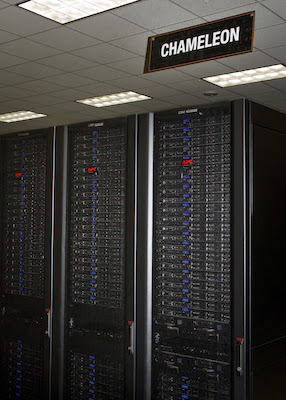
\includegraphics[width=0.5\columnwidth]{images/chameleon/Chameleon2.jpeg}
\caption{Chameleon Cloud Racks}
\end{figure}

\subsection{Network}\label{network}

Networking is changing rapidly, and the network fabric is as much a part
of the research focus of Chameleon as the compute or storage. For the
Chameleon network, every switch in the research network is a fully
OpenFlow compliant programmable Dell S6000-ON switch. Each node connects
to this network at 10 Gbps, and each unit~uplinks with 40Gbps per rack
to the Chameleon core network. The core switches (Dell S6000-ON) are
connected by~40 Gbps Ethernet links, which connect to the backbone
100Gbps services at both UC and TACC.~A Fourteen Data Rate (FDR)
Infiniband network (56Gbps) is also deployed on one SCU to allow
exploration of alternate networks.


\subsection{Shared Storage}\label{shared-storage}

While storage is dynamically provisioned to researchers to be used as an
experiment needs within the SCUs, Chameleon also provides a shared
storage system. The shared storage provides more than 3.6PB of raw disk
in the initial configuration, which is partitioned between a file system
and an object store that is persistent between experiments. The shared
storage is comprised of four Dell R630 servers with 128 GiB of RAM, four
MD3260 external drive arrays, and six MD3060e drive expansion chassis,
populated by 600 6TB near line SAS drives. The system also includes a
dozen PowerEdge R630 servers as management nodes to provide for login
access to the resource, data staging, system monitoring, and hosting
various OpenStack services.


\subsection{Heterogeneous Compute
Hardware}\label{heterogeneous-compute-hardware}

The heterogeneous hardware includes various technologies: GPU and FPGA
accelerators, SSD and NVMe storage, low-power ARM, Atom, and Xeon
systems-on-a-chip. With the exception of the low-power
systems-on-a-chip, each of the additional nodes is a Dell PowerEdge R730
server with the same CPUs as the R630 servers in our SCUs.

The two storage hierarchy nodes have been designed to enable experiments
using multiple layers of caching: they are configured with 512 GiB of
memory, two Intel P3700 NVMe of 2~TB each, four Intel S3610 SSDs of 1.6
TB each, and four 15K SAS HDDs of 600 GB each.

The GPU offering consists of two K80 GPU nodes, two M40 GPU nodes,
sixteen P100 GPU nodes. These nodes target experiments using
accelerators to improve the performance of some algorithms, experiments
with new visualization systems, and deep machine learning. Each K80 GPU
node is upgraded with an NVIDIA Tesla K80 accelerator, consisting of two
GK210 chips with 2496 cores each (4992 cores in total) and 24 GiB of
GDDR5 memory. Each M40 node is upgraded with an NVIDIA Tesla M40
accelerator, consisting of a GM200 chip with 3072 cores and 12 GiB of
GDDR5 memory. The P100 nodes have two GPU cards installed each,
providing 32 P100 GPUs in total. The P100 GPUs utilize GP100 chips
providing 3584 cores, with 16 GiB GDDR5 RAM in each card.~In order to
make it easy for users to get started with the GPU nodes, we have
developed a~\href{https://www.chameleoncloud.org/appliances/21/}{CUDA
appliance} that includes NVIDIA drivers as well as the CUDA framework.

\begin{longtable}[]{@{}llllll@{}}
\toprule
GPU & Chip & Cores per GPU & RAM per GPU & GPU per node & \# of
nodes\tabularnewline
Tesla K80 & GK 210 & 2496 $\times$ 2 & 24 GiB GDDR5 & 1 & 2\tabularnewline
Tesla M40 & GM 200 & 3072 & 12 GiB GDDR5 & 1 & 2\tabularnewline
Tesla P100 & GP100 & 3584 & 16 GiB GDDR5 & 2 & 16\tabularnewline
\bottomrule
\end{longtable}

The four FPGA nodes have a~Nallatech 385A board with an Altera Arria 10
1150 GX FPGA (up to 1.5 TFlops), 8 GiB DDR3 on-card memory, and dual
QSFP 10/40 GbE support. The Chameleon
\href{https://www.chameleoncloud.org/docs/bare-metal-user-guide/fpga/}{FPGA
User Guide}~provides details for conducting experiments on this
hardware.

The low-power systems are comprised of 8 low power Xeon servers (HP
ProLiant m710p with one 4-core Intel Xeon E3-1284L v4 processor), 8 Atom
servers (HP ProLiant m300 with one 8-core Intel Avoton-based System on a
Chip), and 24 ARM servers (HP ProLiant m400 with one 8-core AppliedMicro
X-gene System on a Chip). These are all delivered in a single HP
Moonshot 1500 chassis.

For more information on how you can reserve these nodes, see the
\href{https://www.chameleoncloud.org/docs/bare-metal-user-guide/\#heterogeneous_hardware}{heterogeneous
hardware section} of the bare metal user's guide.


\subsection{Live updates}
You can browse detailed information about the resources
offered~for bare metal reconfiguration in our
\href{https://www.chameleoncloud.org/user/discovery/}{Resource Discovery
Portal}.


\chapter{Getting Started}
\label{C:cc-start}

\FILENAME

We describe how you can get access to chameleon cloud under the
assumption that you are a student or a researcher that joins an
existing project on Chameleon cloud. You will need to follow the
following steps:

\section*{Step 1: Create~a Chameleon~account}

To get started using Chameleon you will need to
\href{https://www.chameleoncloud.org/register}{create a user account}.

You will be asked to agree to the
\href{https://www.chameleoncloud.org/terms/view/chameleon-user-terms/}{Chameleon
  terms and conditions} which, among others, ask you to acknowledge
the use of Chameleon in your publications. 

Acknowledgement of support from the Chameleon project and the
National Science Foundation should appear in any publication of
material, whether copyrighted or not, that describes work which
benefited from access to Chameleon cyberinfrastructure resources. The
suggested acknowledgement is as follows: ``Results presented in this
paper were obtained using the Chameleon testbed supported by the
National Science Foundation''.

\begin{IU}
  As part of creating an account you may request PI status. However
  you are not a PI as you will be joining a project.
\end{IU}

\section*{Step 2: Create or join a project}

To use Chameleon, you will need to be associated with a
\href{https://www.chameleoncloud.org/docs/user-faq/\#toc-how-do-i-apply-for-a-chameleon-project-}{project}
that is assigned an
\href{https://www.chameleoncloud.org/docs/user-faq/\#toc-what-are-the-project-allocation-sizes-and-limits-}{allocation}.
This means that you either need to

\begin{enumerate}

\item \textbf{\href{https://www.chameleoncloud.org/user/projects/new/}{apply
for a new project}} or 

\item
\textbf{\href{https://www.chameleoncloud.org/docs/user-faq/\#toc-my-pi-professor-colleague-already-has-a-chameleon-project-how-do-i-get-added-as-a-user-on-the-project-}{ask
the PI of an existing Chameleon project to add you}.}

\end{enumerate}

A project is headed by a project PI, typically
\href{https://www.chameleoncloud.org/docs/user-faq/\#toc-who-is-eligible-to-be-chameleon-pi-and-how-do-i-make-sure-that-my-pi-status-is-reflected-in-my-profile-}{a
faculty member or researcher scientist at a scientific institution}. If
you are a student we recommend that you ask your professor to work with
you on creating a project. Please note that you must not create a
project by yourself and that you indeed need to work with your
professor. 

In case you need to do a project application typically consists of
about one paragraph description of the intended research and takes one
business day to process.

Enrolling you into an existing research or class project depends on
the time availability of the project lead or professor of your
class. It is important that you communicate your chameleon cloud
account name to the project lead so they can easily add you. Make sure
you really give them only your chameleon account name and potentially
your organizational e-mail, Firstname, and Lastname so they can check
you are eligible to get access. 

\begin{IU}
Indiana University students that take the e516 and e616 classes will
have to fill out a google form in which they communicate the chameleon
cloud name. You can already apply for an account name, but do not
apply for a project. If you nevertheless apply for a project, we will
hear from the administrators and you will receive a point deduction.
\end{IU}

\section*{Step 3: Start using Chameleon!}\label{using-chameleon}

Now that you have enrolled and once you are added to the project by your
project lead you can start using chameleon cloud. However be reminded
that you ought to shut down the resources/VMs whenever they are not in
use to avoid unnecessary charging. Remember the project has imited
time on chameleon and any unused time will be charged against the project.

Chameleon provides two types of resources with links to their respective
users guides below:

\textbf{\href{https://www.chameleoncloud.org/docs/bare-metal-user-guide-old/}{Bare
Metal User Guide}} will tell you how to use Chameleon bare metal
resources which provide strong isolation and allow you maximum control
(reboot to new operating system, reboot the kernel, etc.)

\textbf{\href{https://www.chameleoncloud.org/docs/user-guides/openstack-kvm-user-guide/}{OpenStack
KVM User Guide}} will tell you how to get started with Chameleon's
OpenStack KVM cloud which is a multi-tenant environment providing weak
performance isolation. 

If you have any questions or encounter any problems, you can check out
our \href{https://www.chameleoncloud.org/docs/user-faq/}{User FAQ},
or \href{https://www.chameleoncloud.org/user/help/}{submit a ticket}.

\begin{IU}
As part of the classes you will need to first pass a cloud {\em security}
drivers licence test.  The test is designed so that you think about
gaining access to a VM securely and how to properly secure the
VM. Once passed, access is typically provided by midterm time. You are
not allowed to constantly run VM's and must shut them down if not in
use. You will get point deductions if we detect you do not obey by
this rule. We have access to log files about your VM usage.
\end{IU}


\section{Charge Rates}
\label{C:cc-charge}

It is important to fully understand the charge rates of your VM and storage use.

Chameleon has two types of limitations, introduced to promote fair resource
usage to all:

\begin{description}

\item  [Allocation:] Chameleon projects are limited to a per-project allocation
  currently set to~20,000 service units for 6 months. Allocations can be
  renewed or extended (see
  \href{index.html\#toc-project-and-allocation-management}{Project and
  Allocation Management} section for more details on Chameleon
allocations.)

  \item [Lease:] To ensure fairness to all users, resource reservations (leases)
  are limited to a duration of 7 days. However, an active lease within
  48 hours of its end time can be prolonged by up to 7 days from the
  moment of request if resources are available. To prolong a lease,
  click on the ``Update Lease'' button in the Reservations panel of the
  CHI OpenStack dashboard, and enter the additional duration requested
  in the ``Prolong for'' box including the unit suffix, e.g. ``5d'' for
  5 days or ``30m'' for 30 minutes. If there is an advance reservation
  blocking your lease prolongation that could potentially be moved,
  you can interact through the users mailing list to coordinate with
  others  users.~Additionally, if you know from the start that your
  lease will  require longer than a week and can justify it, you can
  \href{https://www.chameleoncloud.org/user/help/ticket/new/}{contact
    Chameleon staff via the ticketing system} to request a one-time
  exception to create a longer lease. The lease must be requested by
  the PI.

\end{description}

\subsection{Service Units}

Chameleon allocations can consist of several components of the system.
Users can request allocation of individual compute nodes, storage
servers, or complete Scalable Compute Units (SCUs) which contain compute
servers, storage nodes, and an open flow switch.

Compute servers are allocated in Service Units (SUs), which equates to
one hour of wall clock time on a single server (for virtual machines, an
SU is 24 cores with up to 128GB of RAM). Note this unit differs from
traditional HPC or cloud service units that are charged in core-hours; a
Chameleon SU is a full server, as the type of experiments and
performance measurements users may wish to do may be contaminated by
sharing nodes.

Storage servers are also charged in SUs, at 2x the rate of compute
servers (i.e., 1 hour allocation of 1 storage server == 2 SUs). SCUs are
charged at the rate of 50 SUs per wall clock hour (42 compute servers, 4
storage nodes, plus one OpenFlow switch).

An allocation may make use of multiple SCUs, up to the size of the full
testbed.

For example, a user wishing to provision a 10 node cluster +1 storage
server for a 1 week experiment should budget
\texttt{{[}(10\ +\ 2)\ SUs\ per\ hour{]}\ *\ {[}7\ days\ *\ 24\ hours/day{]}\ =\ 2,016\ SUs}
for that experiment.

SUs are charged the same regardless of use case. Hence, whether asking
for bare metal access, virtual machine access, or use of default images,
the charge is the same --- you are charged for the fraction of the
resource your experiment occupies, regardless of the type of the
experiment.

The basic principle for charging service units for Chameleon resources
is to evaluate the amount of time a fraction of the resource is
unavailable to other users. If a reservation is made through the portal
for a particular date/time in the future, the user will be charged for
this time regardless of whether the reservation is actually used, as the
Chameleon scheduling system will have to drain the appropriate part of
the system to satisfy the reservation, even if the nodes requested are
not actually used. A reservation request may be cancelled in which case
no charges will apply.

\subsection{Project Allocation Size}

CUrrently Chameleon is operating on a ``soft allocation
model'' where each project, if approved, will receive a startup
allocation of 20,000 SUs for six months that can be both recharged
(i.e., more SUs can be added) and renewed (i.e., the duration can be
extended) via submitting a renew/recharge request. This startup
allocation value has been designed to respond to both PI needs (i.e.,
cover an amount of experimentation needed to obtain a significant
result) and balance fairness to other users (it represents roughly 1\%
of testbed six months' capacity). Requests for these startup projects
will receive a fast track internal review (i.e., users can expect them
to be approved within a few days).

A PI can apply for multiple projects/allocations; however, the number of
held allocations will be taken into account during review.

As our understanding of user need grows we expect the Chameleon
allocation model to evolve towards closer reflection of those needs in
the form of more differentiated allocations that will allow us to give
larger allocations to users for longer time.

\begin{IU}
  Please be mindful to shutting down your VMS when not in use as even VMs 
  that do not do any calculations get charged. In past classes we had students 
  that did not shut down their VMs and within 2 weeks used up all SUs 
  for the entire class of 70 students. We like to avoid this. In future cases 
  we will assign the grade ``F'' to such students, as is customary also 
  in other universities.
\end{IU}


\section{OpenStack Virtual Machines}
\label{C:cc-guide}

\FILENAME\

OpenStack is an Infrastructure as a Service (IaaS) platform that allows
you to create and manage virtual environments. Chameleon provides an
installation of OpenStack version 2015.1~(Kilo)~using the~KVM
virtualization technology.

Since the KVM hypervisor is used on this cloud, any virtual machines you
upload must be compatible with KVM.

This tutorial provide basic information about how to use the OpenStack
web interface and provides some information specific to using OpenStack
KVM on Chameleon.

\subsection{Web Interface}\label{web-interface-horizon}

An easy way to use OpenStack KVM on Chameleon~is via
the~\href{https://openstack.tacc.chameleoncloud.org/dashboard}{OpenStack
  web interface} also known as Horizon. You log into the web interface
using your Chameleon username and password. If you change your
Chameleon password in the portal, that change will propagate to the
OpenStack KVM interface~in about 5 minutes.

The initial log in page appears as:

\begin{center}
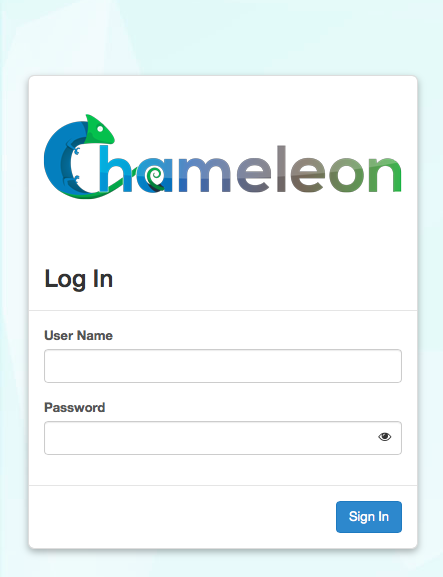
\includegraphics[width=0.3\columnwidth]{images/chameleon/chameleon-login.png}
\end{center}

After a successful log in, you will see the Overview page as shown
below. This page provides a summary of your current and recent usage and
provides links to various other pages. Most of the tasks you will
perform are done via the menu on the lower left and will be described
below. One thing to note is that on the left, your current project is
displayed. If you have multiple Chameleon projects, you can change which
of them is your current project. All of the information displayed and
actions that you take apply to your current project. So in the screen
shot below, the quota and usage apply to the current project you have
selected and no information about your other projects is shown.

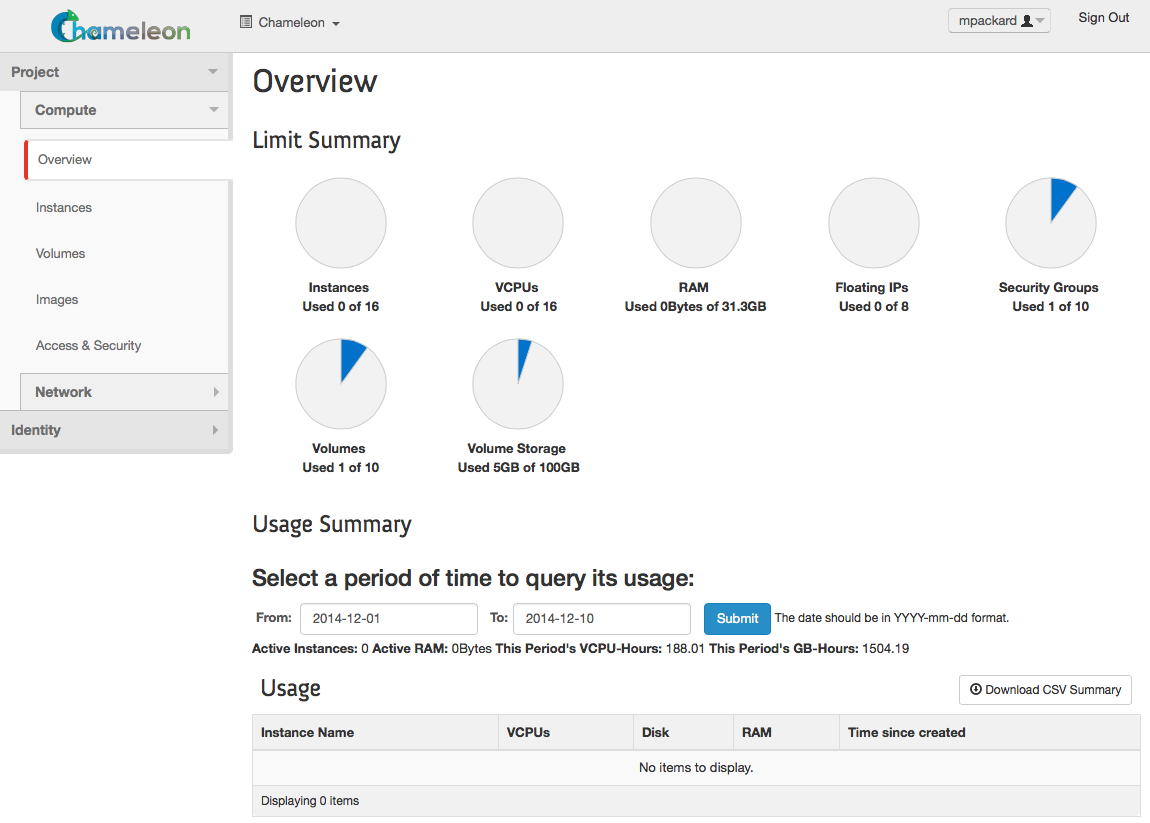
\includegraphics[width=0.8\columnwidth]{images/chameleon/openstack_alamo_overview.png}

\subsubsection{Managing Virtual Machine Instances}\label{managing-virtual-machine-instances}

One of the main activities you'll be performing in this web interface is
the management of virtual machines, or instances. You do this via the
Instances page that is reachable from the menu in the lower left of the
Overview page. An example Instances page is shown below. For instances
that you have running, you can click on the name of the instance to get
more information about it and to access the VNC interface to the
console. The dropdown menu to the left of the instance lets you perform
a variety of tasks such as suspending, terminating, or rebooting the
instance.

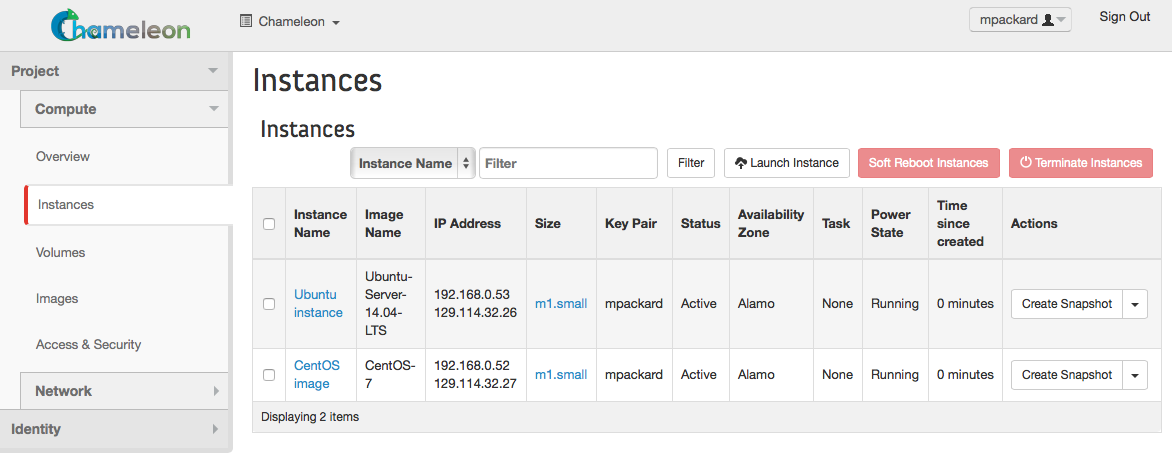
\includegraphics[width=0.8\columnwidth]{images/chameleon/openstack_alamo_instances.png}

The Instances page also lets you create new virtual machines by using
the `Launch Instance' button in the upper-right. When you click this
button, a dialog window pops up. In the first `Details' tab, you select
the `Instance Boot Source' of the instance, which is either an `Image',
a `Snapshot' (an image created from a running virtual machine), or a
`Volume' (a persistent virtual disk that can be attached to a virtual
machine). If you select `Boot from image', the Image Name dropdown
presents a list of virtual machine images that we have provided, that
other Chameleon users have uploaded and made public, or images that you
have uploaded for yourself. If you select `Boot from snapshot', the
Instance Snapshot dropdown presents a list of virtual machine images
that you have created from your running virtual machines.

On the Details tab, you also provide a name for this instance (to help
you identify instances that you are running), and select the amount of
resources (Flavor) to allocate to the instance. If you select different
flavors from the Flavor dropdown, their characteristics are displayed on
the right.

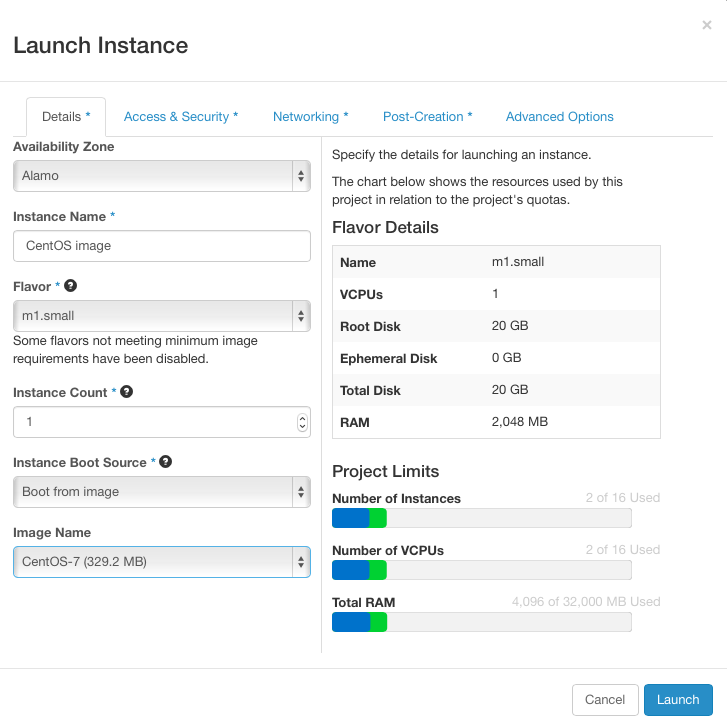
\includegraphics[width=0.8\columnwidth]{images/chameleon/openstack_alamo_launch_details.png}

The next tab is `Access \& Security', where you select an SSH keypair
that will be inserted into your virtual machine. These keypairs can be
uploaded via the main `Access \& Security' section. You will need to
select a keypair here to be able to access an instance created from one
of the public images Chameleon provides. These images are not configured
with a default root password and you will not be able to log in to them
without configuring an SSH key.

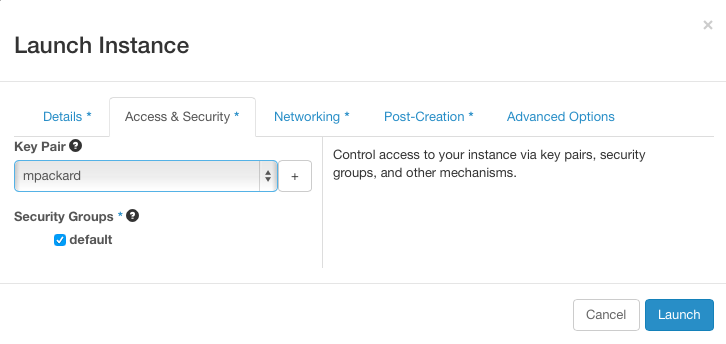
\includegraphics[width=0.8\columnwidth]{images/chameleon/openstack_alamo_launch_access.png}

Next is `Networking', where you select which network should be
associated with the instance. Click the + next to your your project's
private network (PROJECT\_NAME-net), not ext-net.

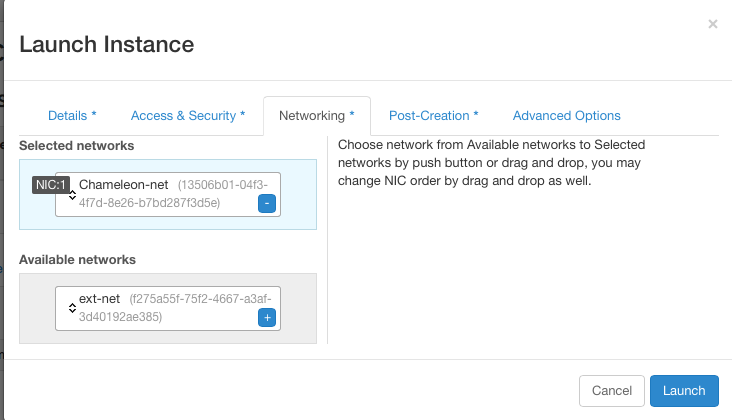
\includegraphics[width=0.8\columnwidth]{images/chameleon/openstack_alamo_networking.png}

Once you do this, you can Launch your instance and the Instances page
will show progress as it starts.

If you would like to assign a public IP address to your VM, you can do
that while it is booting up. Click on the dropdown under \emph{Actions}
and choose \emph{Associate Floating IP}. Choose an IP from the \emph{IP
Address} menu and click \emph{Associate}. If there are no addresses
available, click the + and follow the prompts to add one.

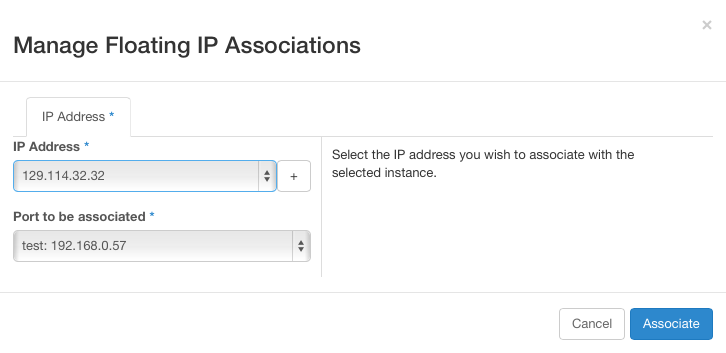
\includegraphics[width=0.8\columnwidth]{images/chameleon/openstack_alamo_floating.png}

OpenStack injects your SSH key into the VM and you can use the
corresponding private SSH key to log in to the VM. You will need to use
the public IP assigned to your VM to connect from outside of Chameleon,
or connect through an existing instance that both a public and private
IP.

\textbf{Note that the images we provide do not allow SSH into the root
account. For root access, SSH into the instance as user `cc' and then
use the \emph{sudo} command to become root.}

We have enabled auto-login for the cc user on the console of our
supported images. This should aid in debugging if you are unable to
reach the instane via ssh for some reason.

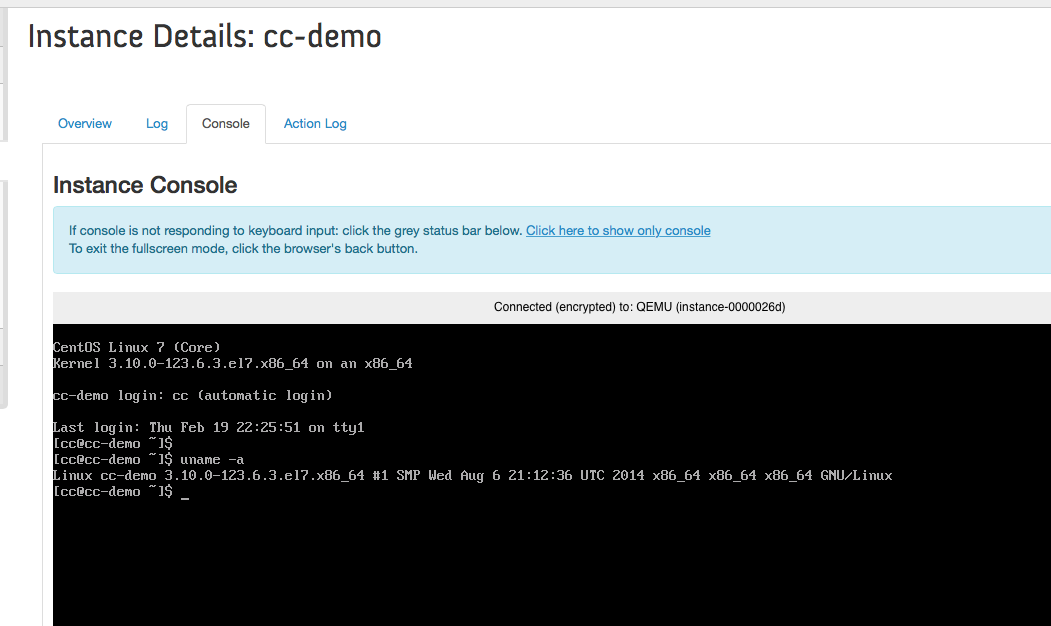
\includegraphics[width=0.8\columnwidth]{images/chameleon/openstack_alamo_console.png}

\subsubsection{Snapshots}\label{snapshots}

The instance list page shown above has an option `Create Snapshot' that
allows you to save a copy of the disk contents of a running virtual
machine. This allows you to start new virtual machines in the future
that are identical to this one and is an easy way to save any changes
you make to a running virtual machine.

\subsubsection{Firewall (Access Security)}\label{firewall-access-security}

Each project has control over their own firewall settings for their
instances. At minimum you'll probably want to allow SSH access so you
can reach your instances.

To enable this traffic, you need to configure the security group used by
your virtual machine. You can see a list of your security groups using
the ``Access \& Security'' link on the left.

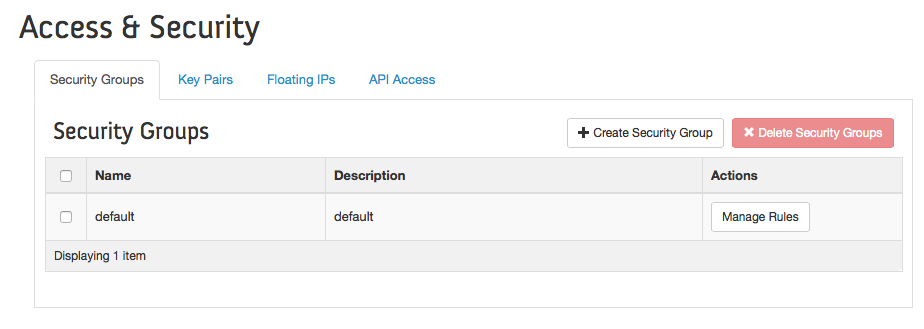
\includegraphics[width=0.8\columnwidth]{images/chameleon/openstack_alamo_security_groups.png}

To edit a security group, click on ``Edit Rules''. This opens a page
showing the existing rules in the security group.

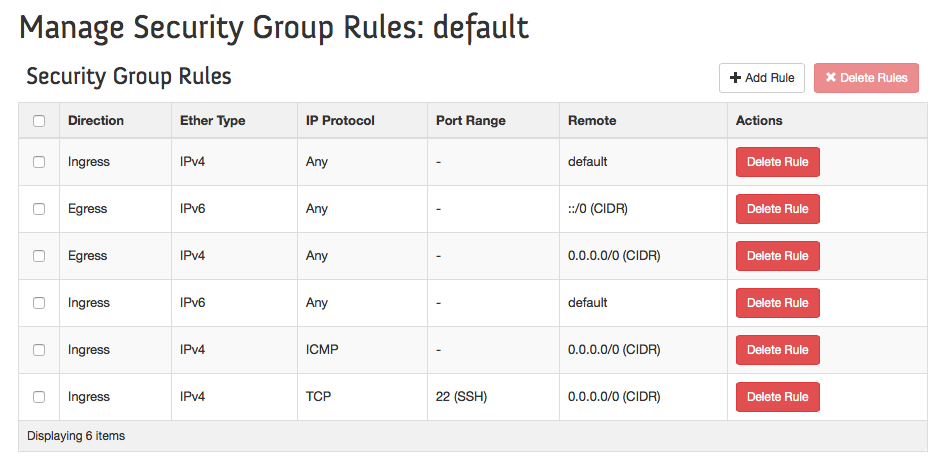
\includegraphics[width=0.8\columnwidth]{images/chameleon/openstack_alamo_edit_rules.png}

Click on ``Add Rule'' and choose the \emph{SSH} rule from the list, and
click \emph{Add}. Modifications are automatically propagated to the
OpenStack cloud. Feel free to add other rules as necessary.

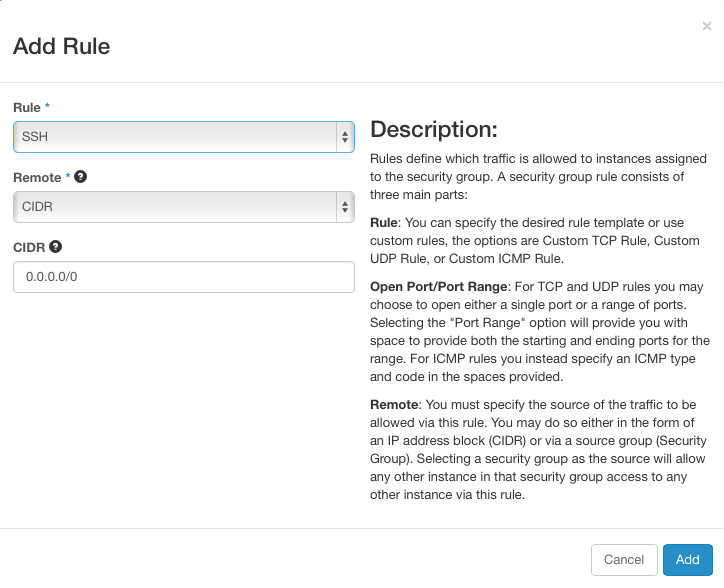
\includegraphics[width=0.8\columnwidth]{images/chameleon/openstack_alamo_add_secgroup_rule.png}

\subsection{OpenStack REST Interfaces}\label{openstack-rest-interfaces}

The OpenStack REST Interfaces are supported on Chameleon over secure
HTTP connections. You can download your OpenStack credentials file from
the web interface via the ``Access \& Security'' link in the left of any
page and then click on the ``API Access'' link on the top.

You can then install the OpenStack command line clients following
\href{http://docs.openstack.org/user-guide/common/cli_install_openstack_command_line_clients.html}{these
instructions}. If using pip, we recommend setting up a virtualenv.

The SSL certificate used by Chameleon~is trusted by most operating
systems, so you shouldn't have to provide any extra options to OpenStack
commands, i.e. ``nova list'' should work.~If your command-line tool
complains about the certificate,
\href{http://curl.haxx.se/docs/caextract.html}{download the Mozilla CA
bundle from the cURL website} and run the OpenStack client tools with
the --os-cacert cacert.pem arguments.

\begin{comment}

 
\subsection{EC2 Interface}\label{ec2-interface}

\begin{IU}
Last time we used the EC2 interface it was broken, thus we no longer
recommend using it
\end{IU}

OpenStack KVM on Chameleon~supports the EC2 interface for programmatic
access. You can download your EC2 credentials from the web interface via
the ``Access \& Security'' link in the left of any page and then click
on the ``API Access'' link on the top. You should see a `Download EC2
Credentials' button on the top-right. Note that you have different EC2
credentials for each Chameleon project you participate in. If you are a
member of multiple Chameleon projects, we request that you use the
corresponding EC2 credentials when starting virtual machines for a
project.

\end{comment}

\subsection{Downloading and uploading data}\label{downloading-and-uploading-data}

You can use the OpenStack command line clients to download data from and
upload data to Chameleon clouds. Configure your environment by following
the ``OpenStack REST Interfaces'' section above, then use the following
commands:

\begin{itemize}
\item
  \verb|glance image-download| to download images and snapshots from
  Glance
\item
  \verb|glance\ image-create| to upload images and snapshots to Glance
\item
  \verb|cinder upload-to-image| to convert a Cinder volume to a
  Glance~image
\item
  \verb|cinder create [--image-id <image-id>] [--image <image>]|
  to create a Cinder volume from a Glance image
\end{itemize}



\FILENAME

\chapter{Horizon Graphical User Interface}

\section{Configure~resources}\label{configureresources}

Once your lease is started, you are almost ready to start an instance.
But first, you need to make sure that you will be able to connect to it
by setting up a key pair. This only has to be done once per user per
project.

Go to Project \textgreater{} Compute \textgreater{} Access \& Security,
then select the Key Pairs tab.

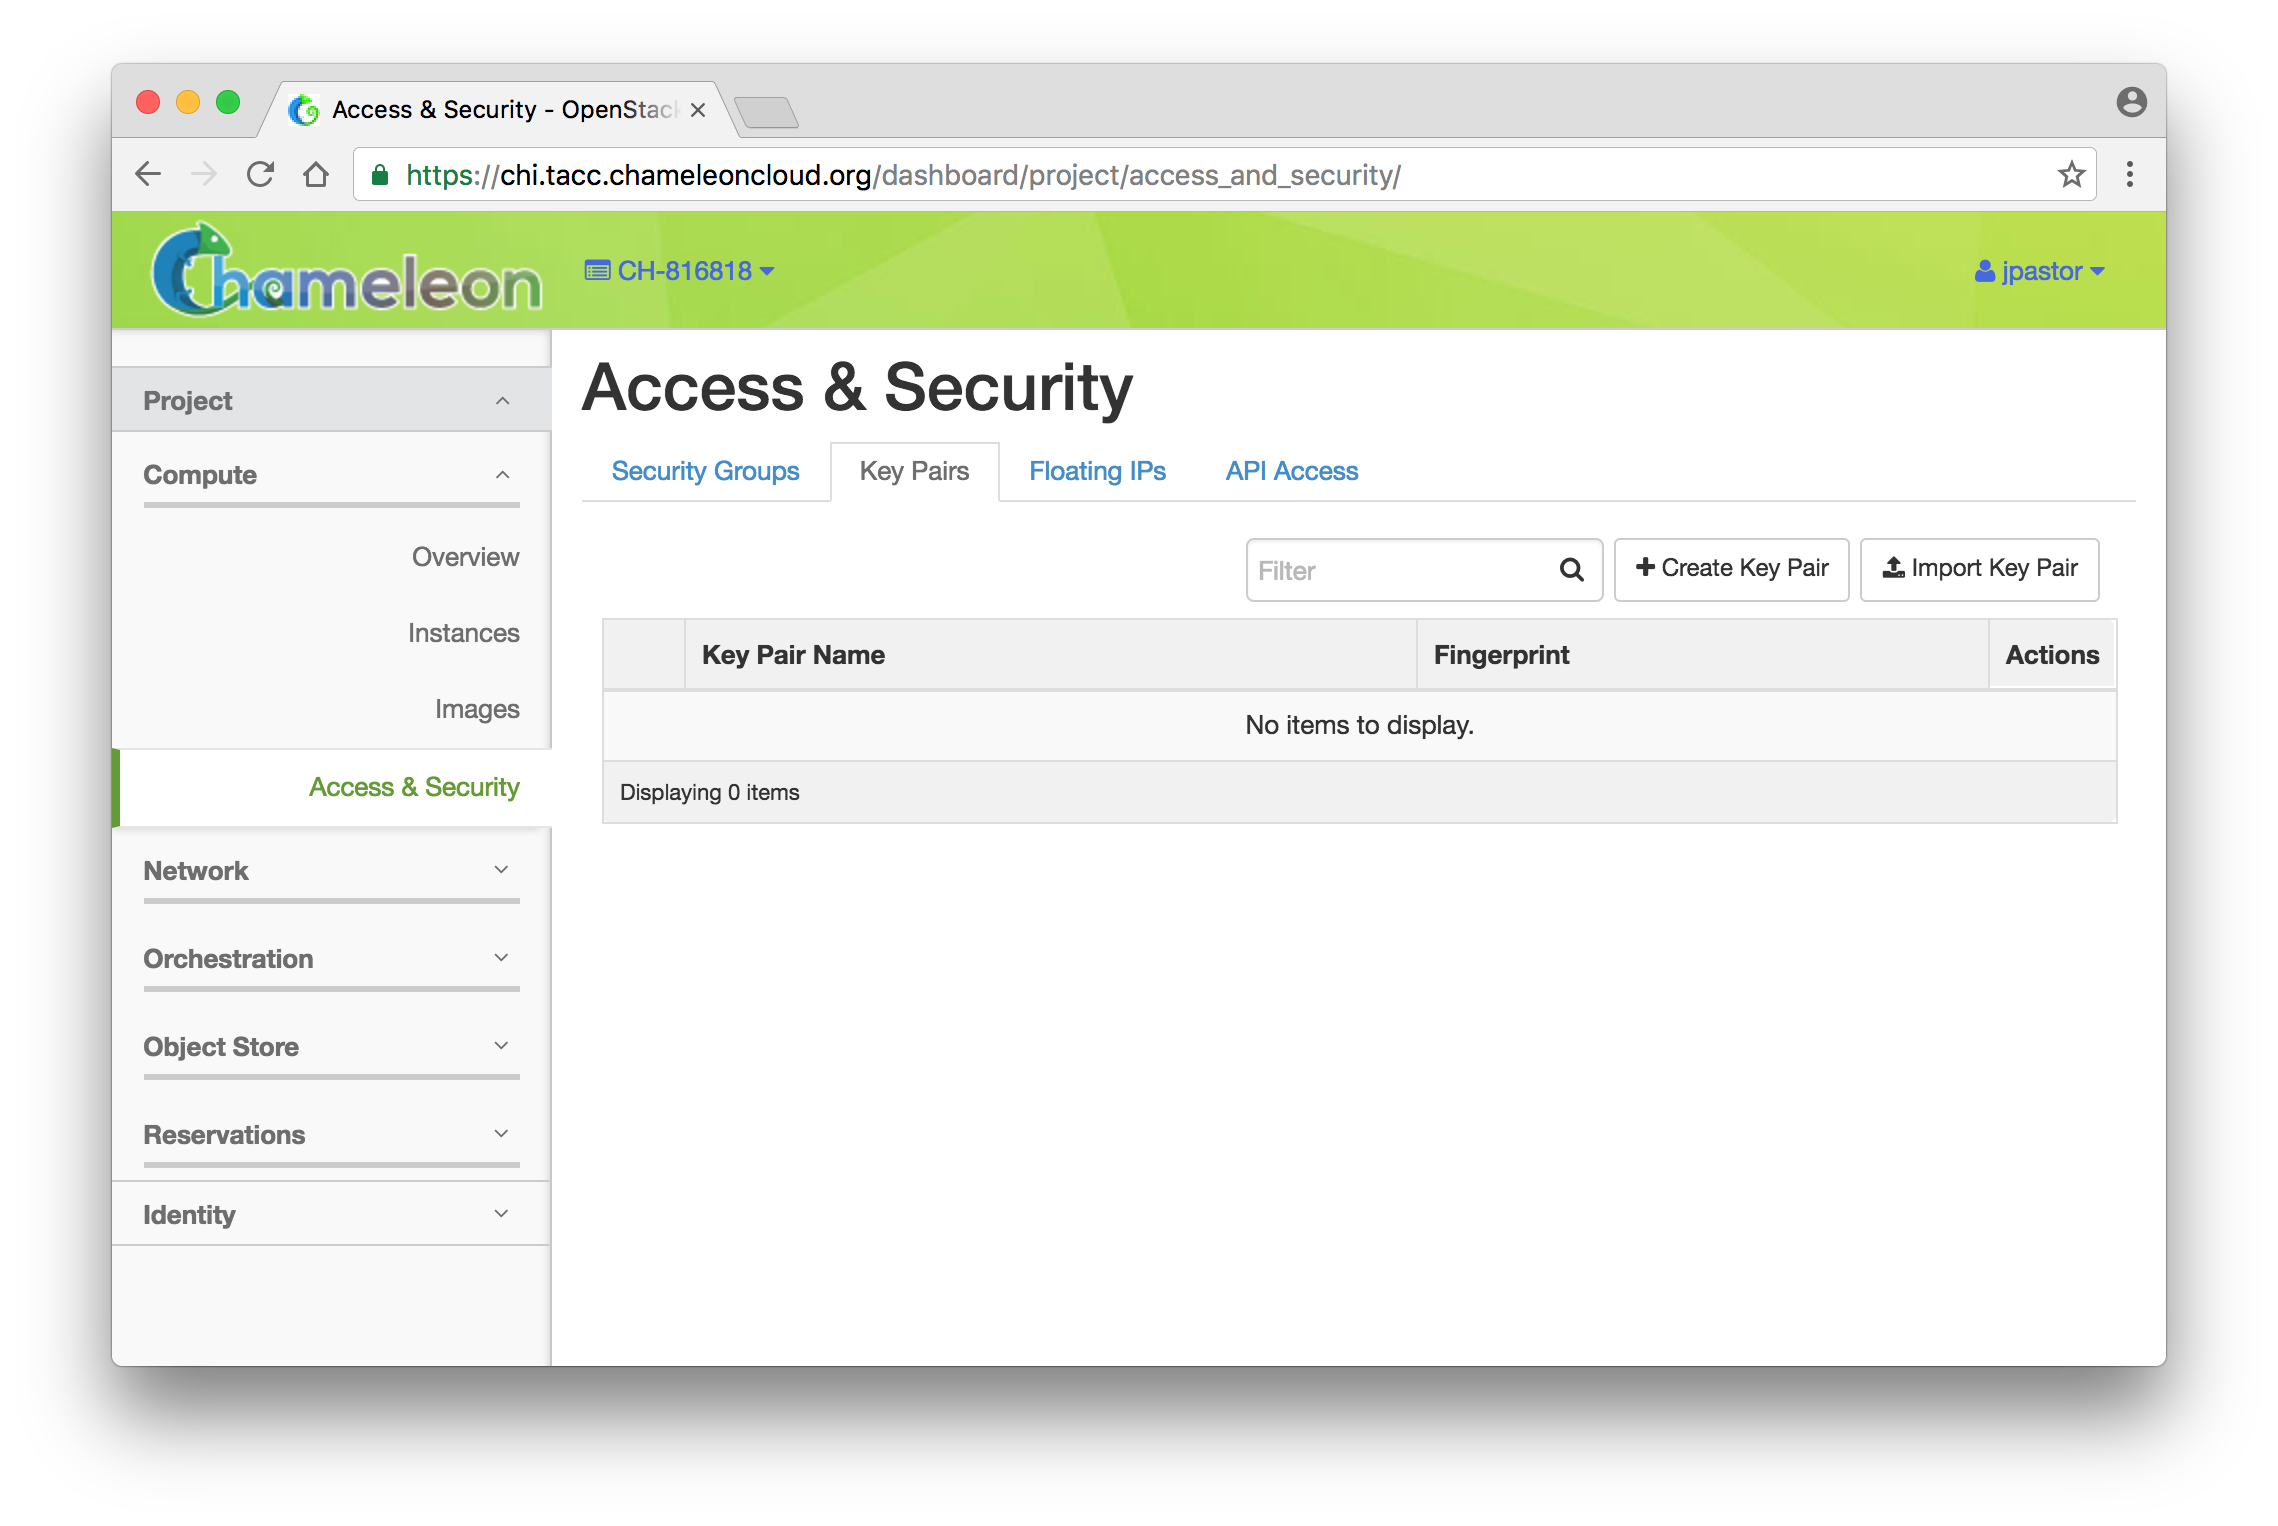
\includegraphics[width=\columnwidth]{images/chameleon/Screen-Shot-2016-10-26-at-14-37-00.png}

Here you can either ask OpenStack to create an SSH key pair for you (via
the ``Create Key'' Pair~button), or, if you already have an SSH key pair
on your machine and are happy to use it, click on ``Import Key Pair''.

If you chose to import a key pair, you will be asked to enter a name for
the key pair, for example laptop. In the ``Public Key'' box, copy the
content of your SSH public key. Typically it will be at
\textasciitilde{}/.ssh/id\_rsa.pub. On Mac OS X, you can run in a
terminal:
~\texttt{cat\ \textasciitilde{}/.ssh/id\_rsa.pub\ \textbar{}\ pbcopy}\\
It copies the content of the public key to your copy/paste buffer. Then
you can simply paste in the ``Public Key'' box.

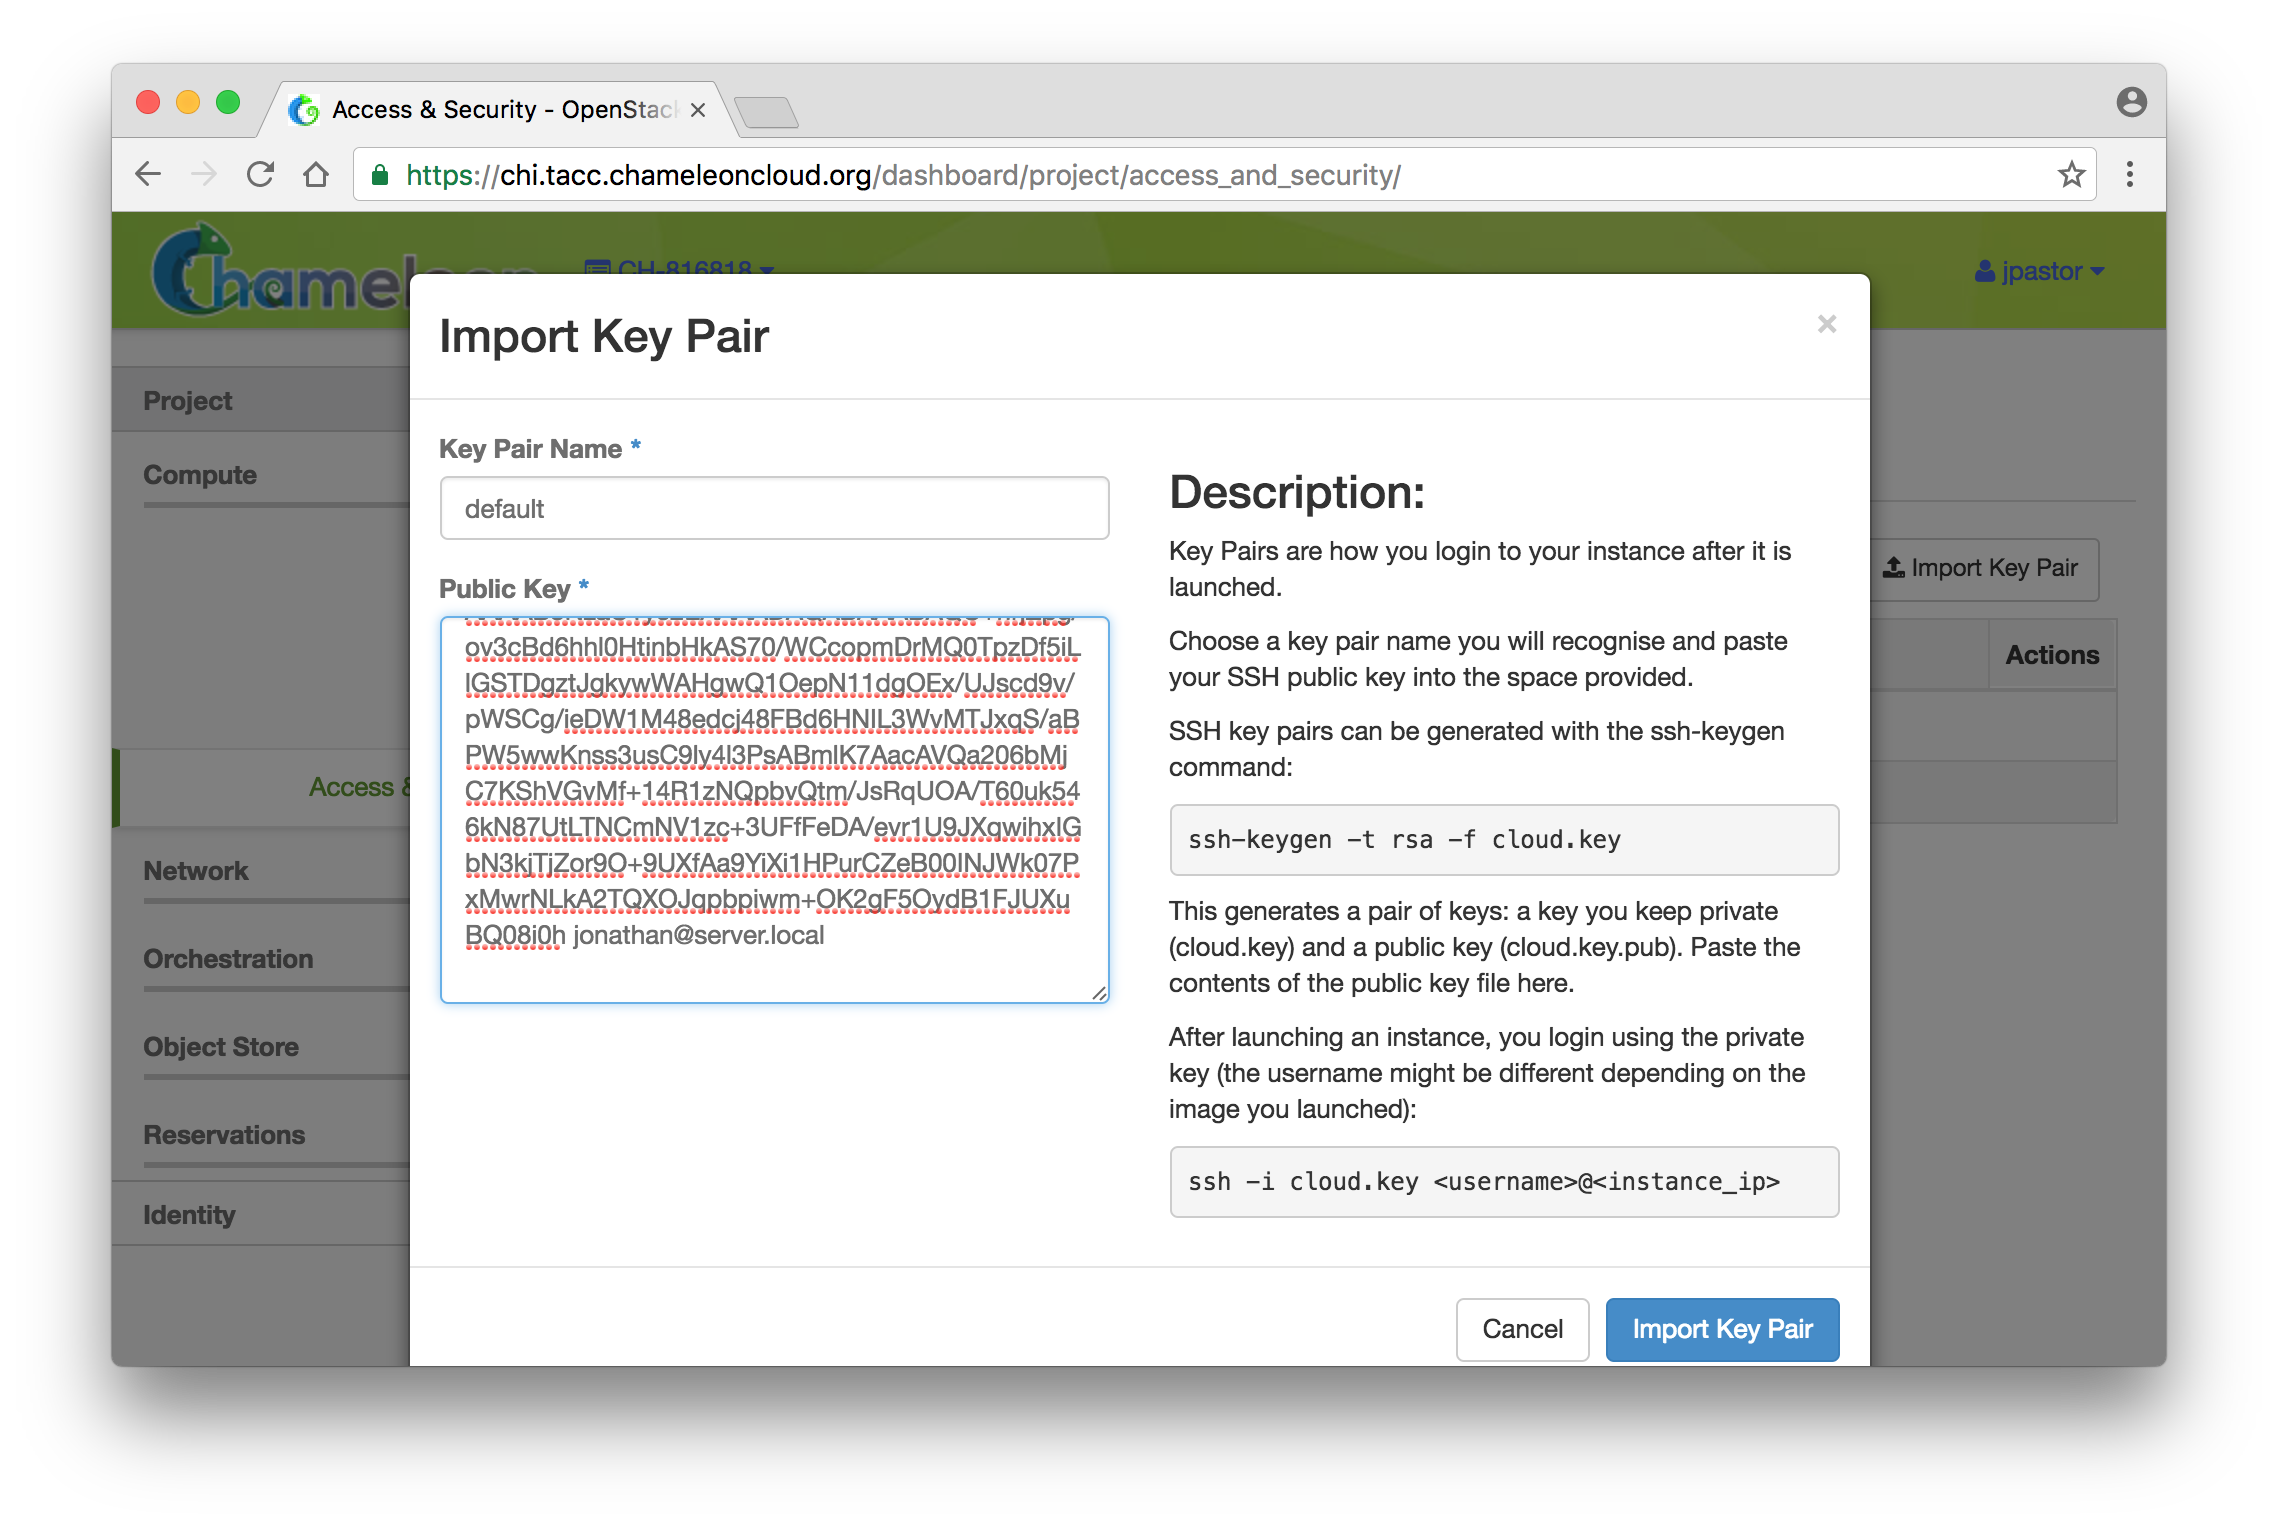
\includegraphics[width=\columnwidth]{images/chameleon/Screen-Shot-2016-10-26-at-14-37-18.png}

Then, click on the blue ``Import Key~Pair'' button. This should show you
the list of key pairs, with the one you just added.

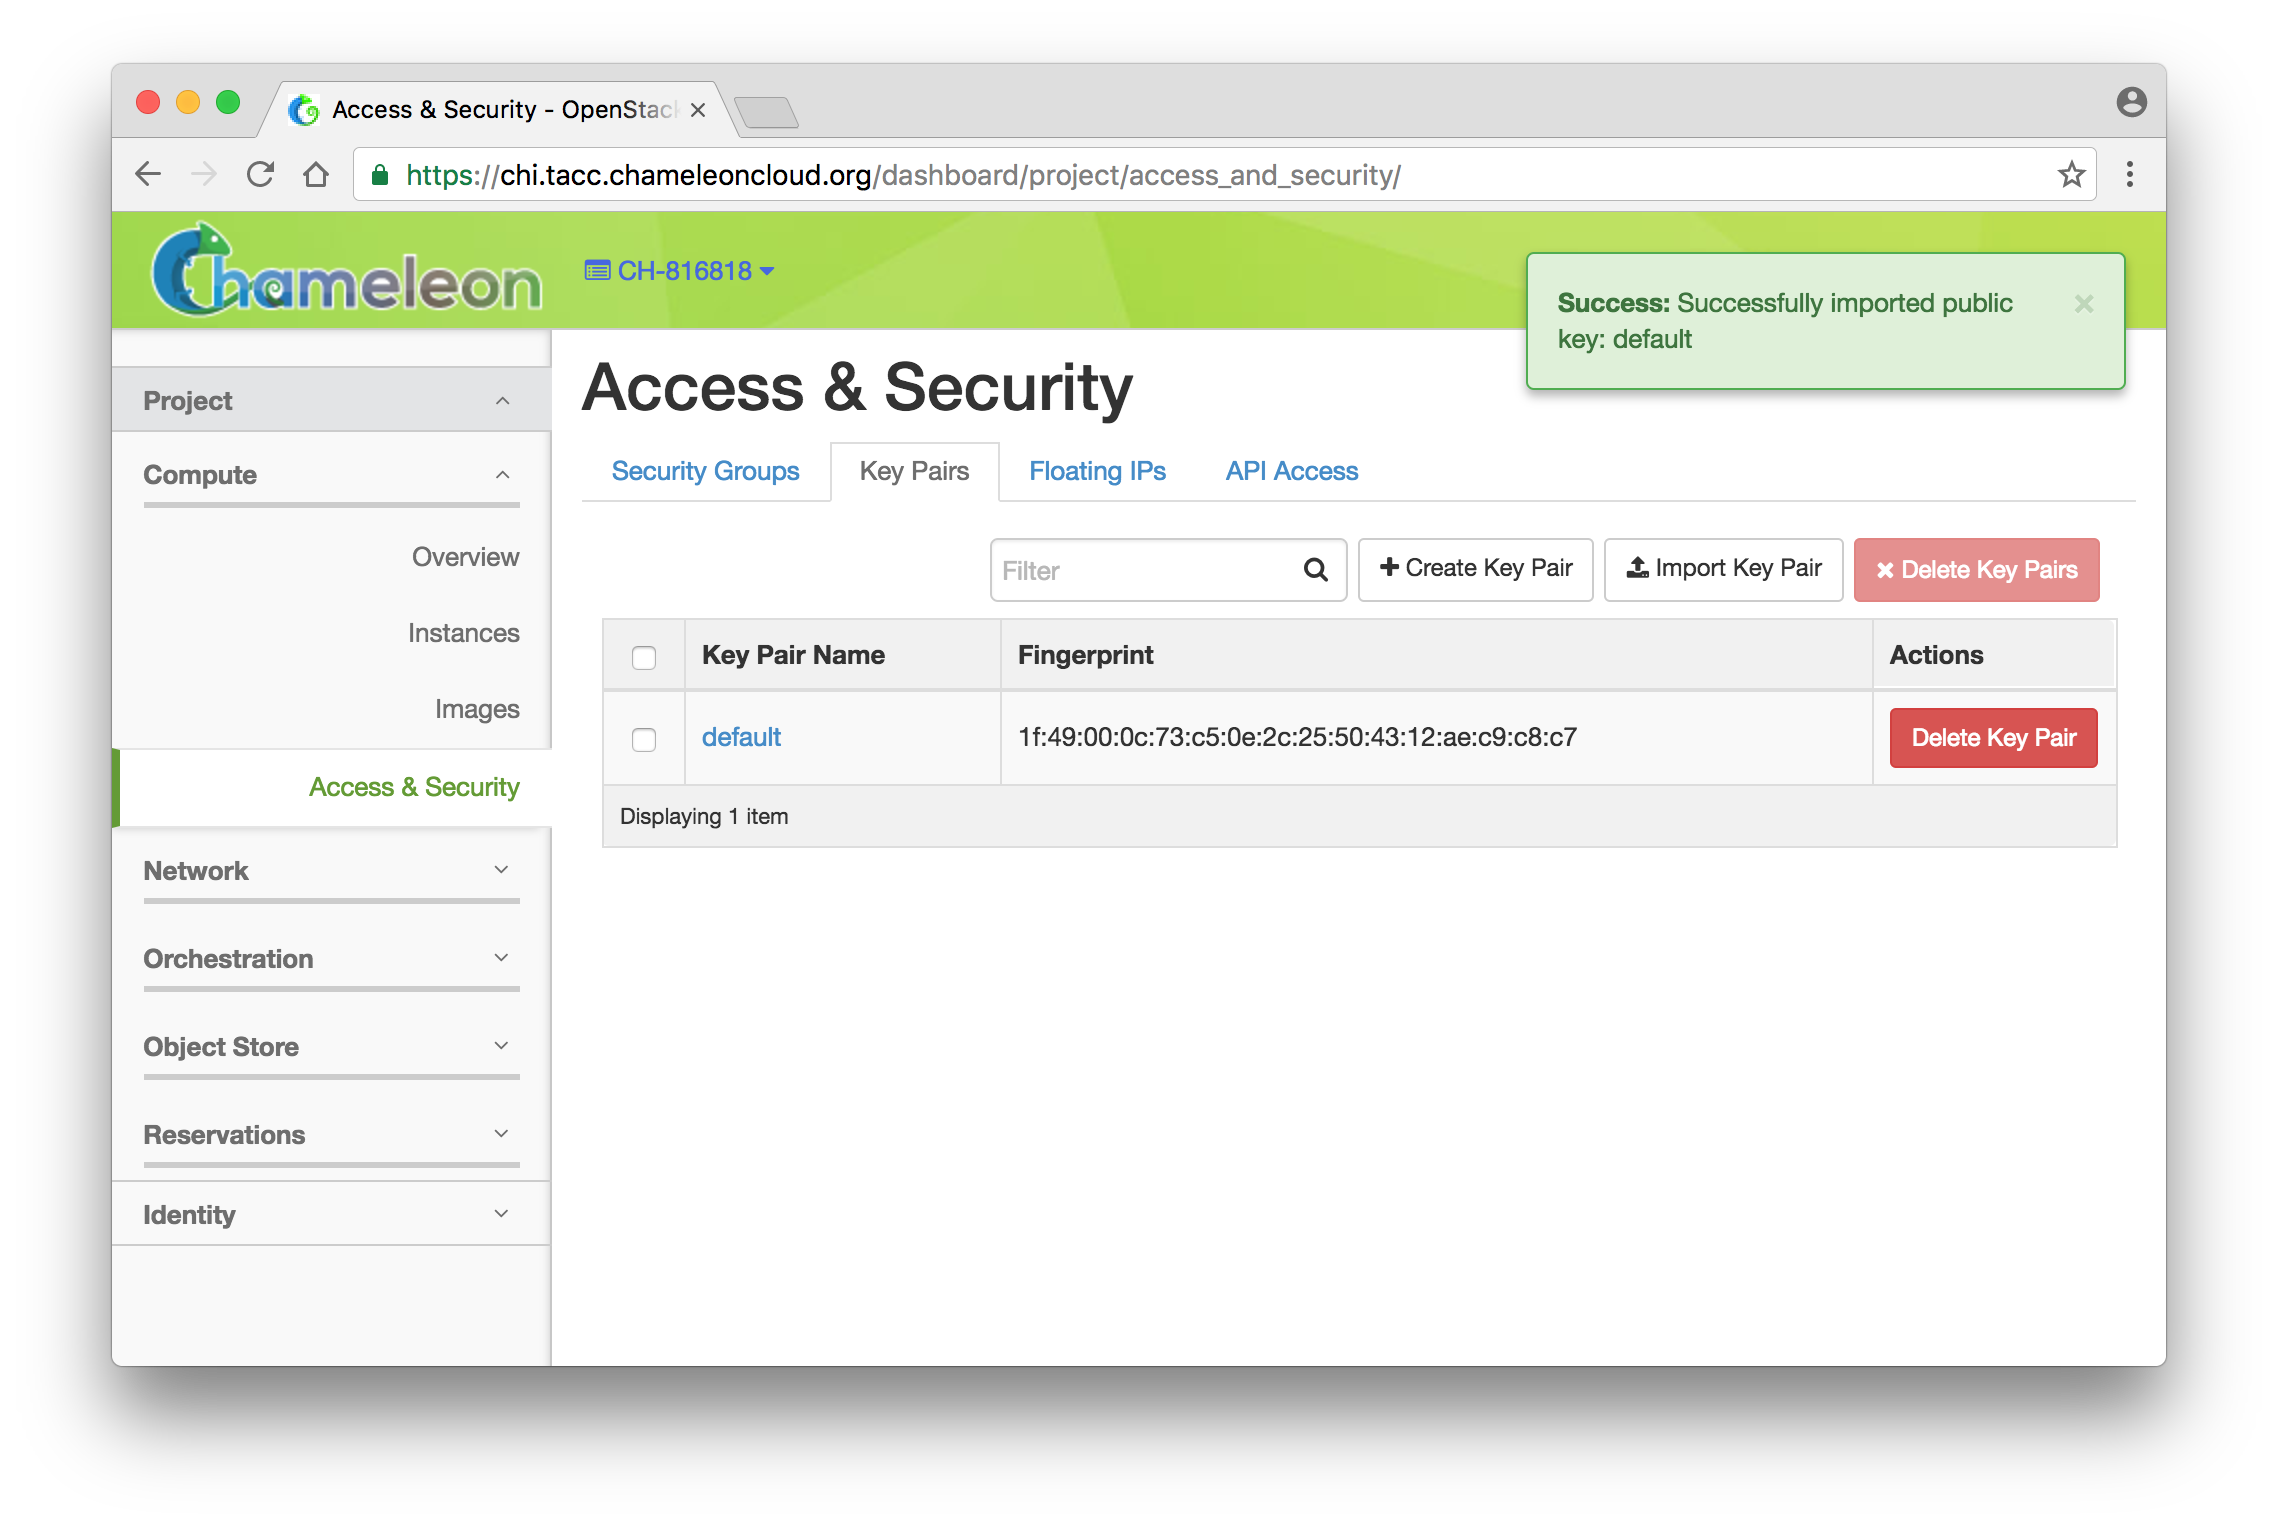
\includegraphics[width=\columnwidth]{images/chameleon/Screen-Shot-2016-10-26-at-14-37-52.png}

For those already familiar with OpenStack, note that Security Groups are
not functional on bare-metal. All instances ports are open to the
Internet and any security group rule you add will not be~respected.

~

Now, go to the ``Instances'' panel.

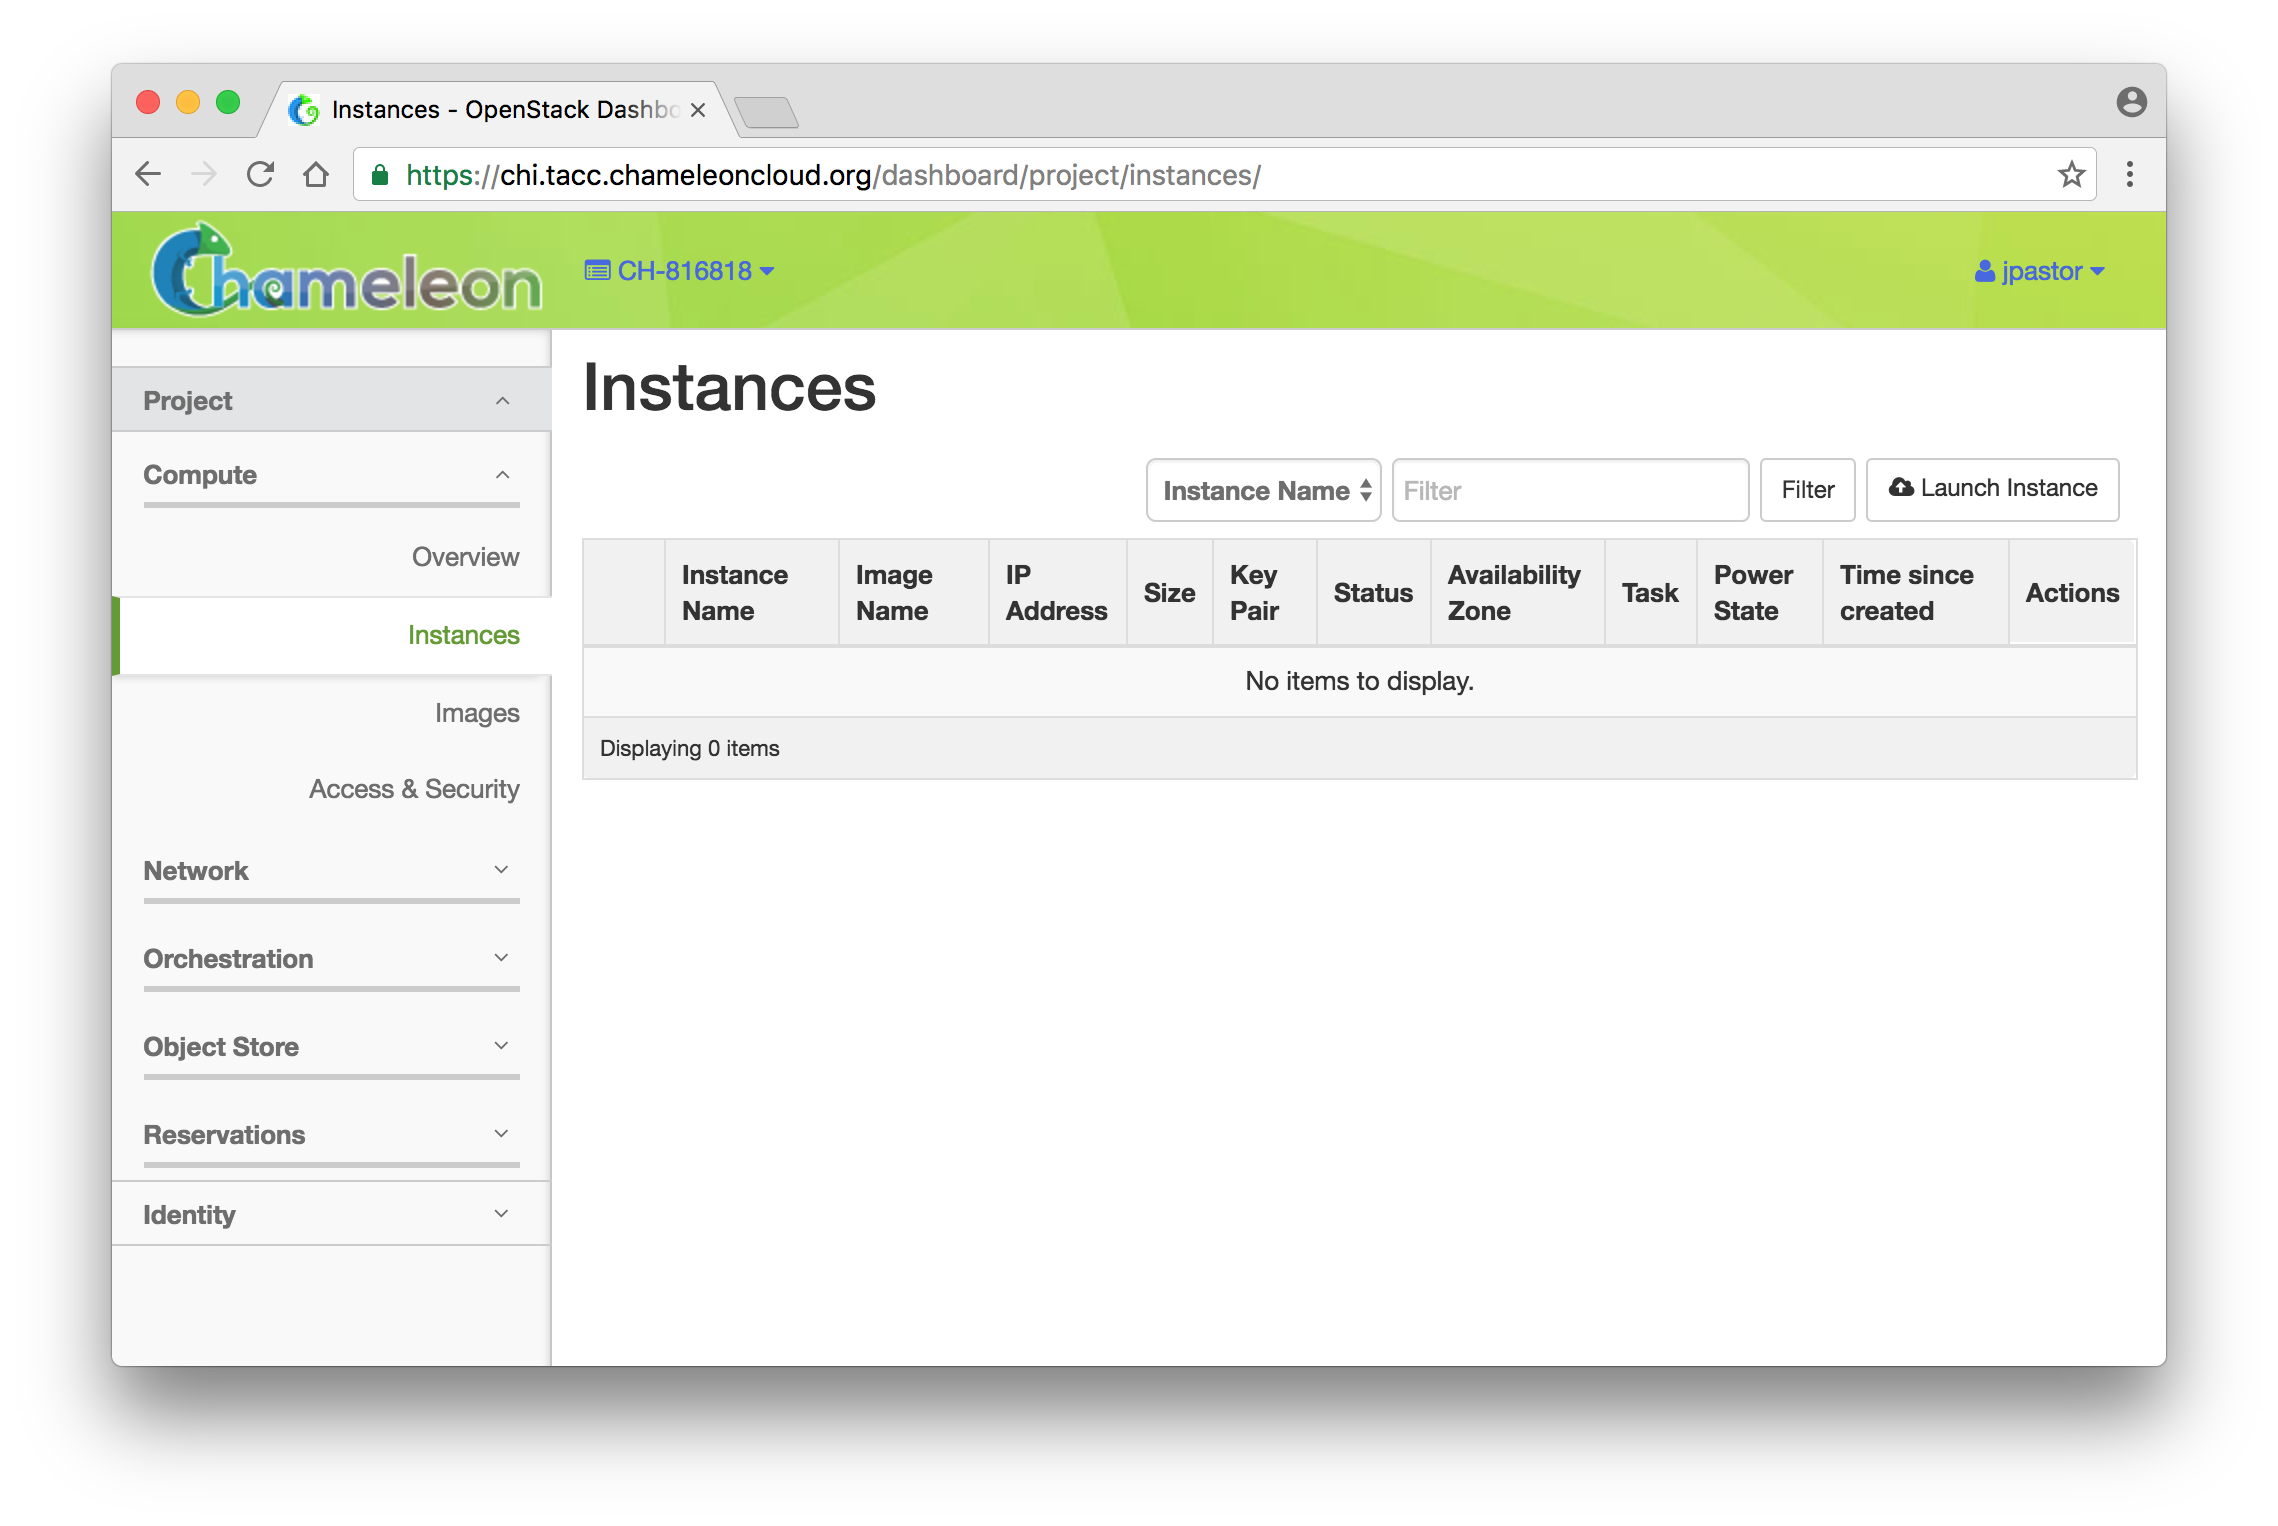
\includegraphics[width=\columnwidth]{images/chameleon/Screen-Shot-2016-10-26-at-14-39-56.png}

Click on the ``Launch Instance'' button in the top right corner. Select
a reservation in the Reservation box, pick an instance name (in this
example my-first-instance) and in~the Image Name list select our default
environment named CC-CentOS7. If you have multiple key pairs registered,
you need to select one in the ``Access \& Security''~tab. Finally, click
on the blue ``Launch'' button.

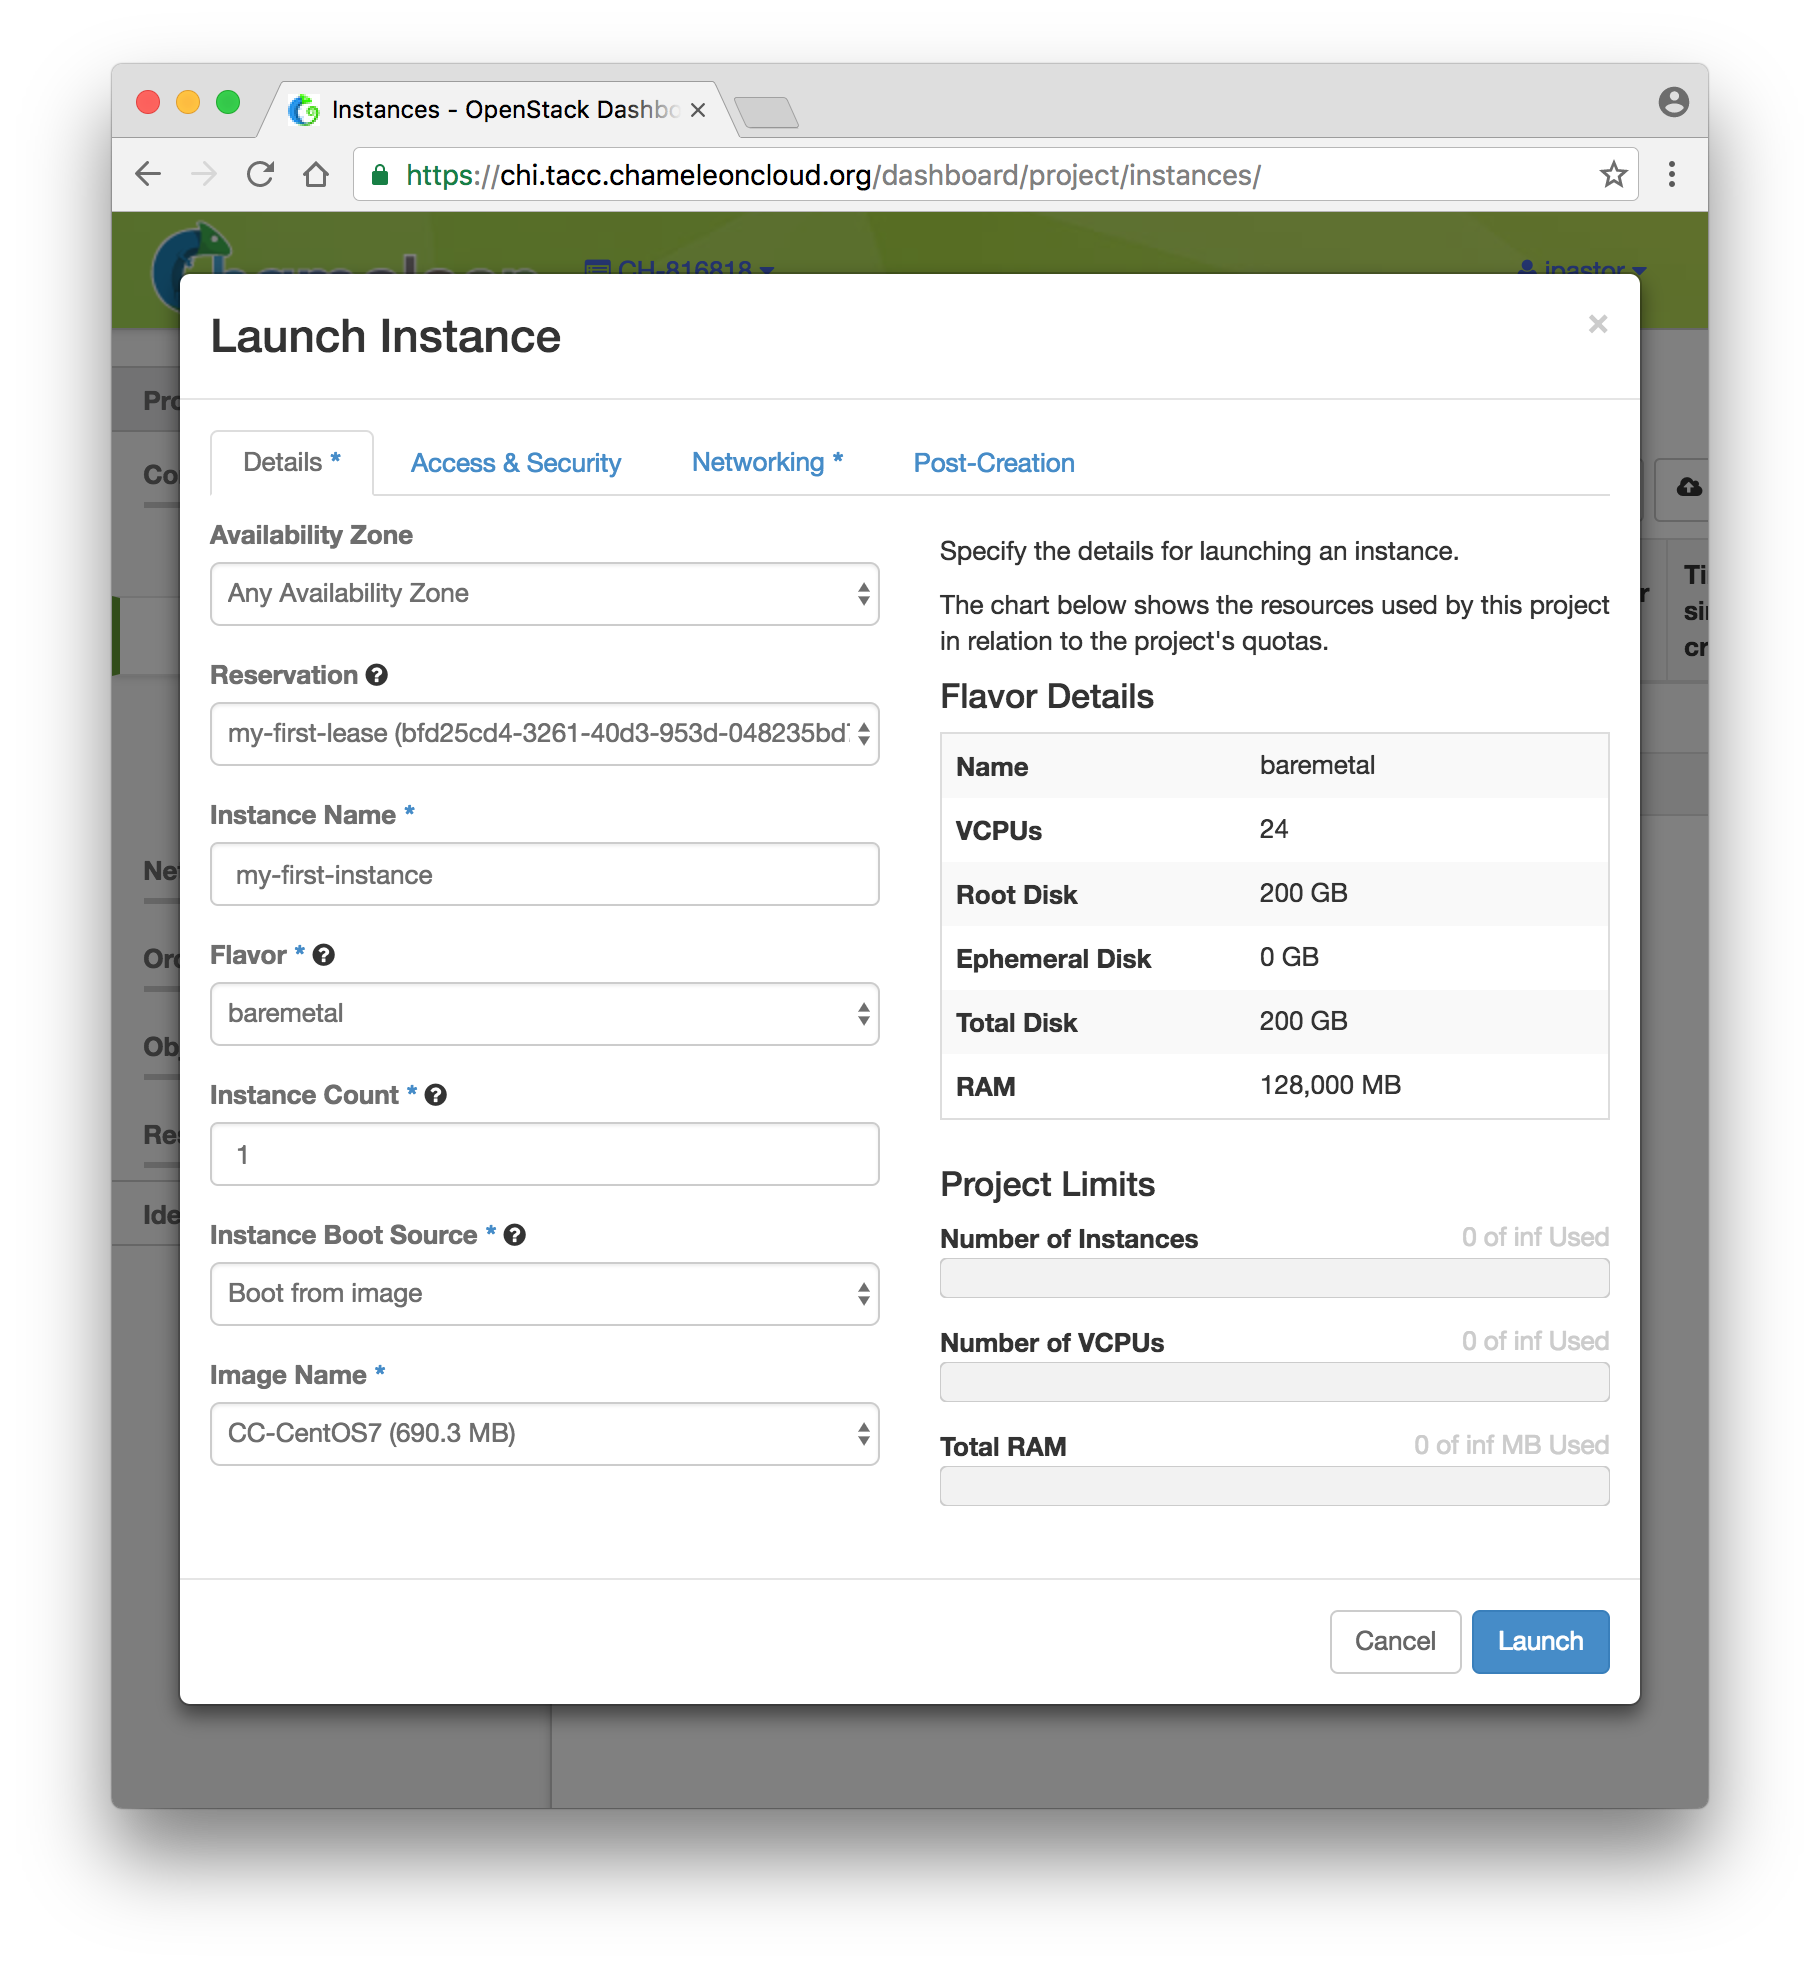
\includegraphics[width=\columnwidth]{images/chameleon/Screen-Shot-2016-10-26-at-14-41-08.png}

The instance will show up in the instance list, at first in Build
status. It takes a few minutes to deploy the instance on bare-metal
hardware and reboot the machine.

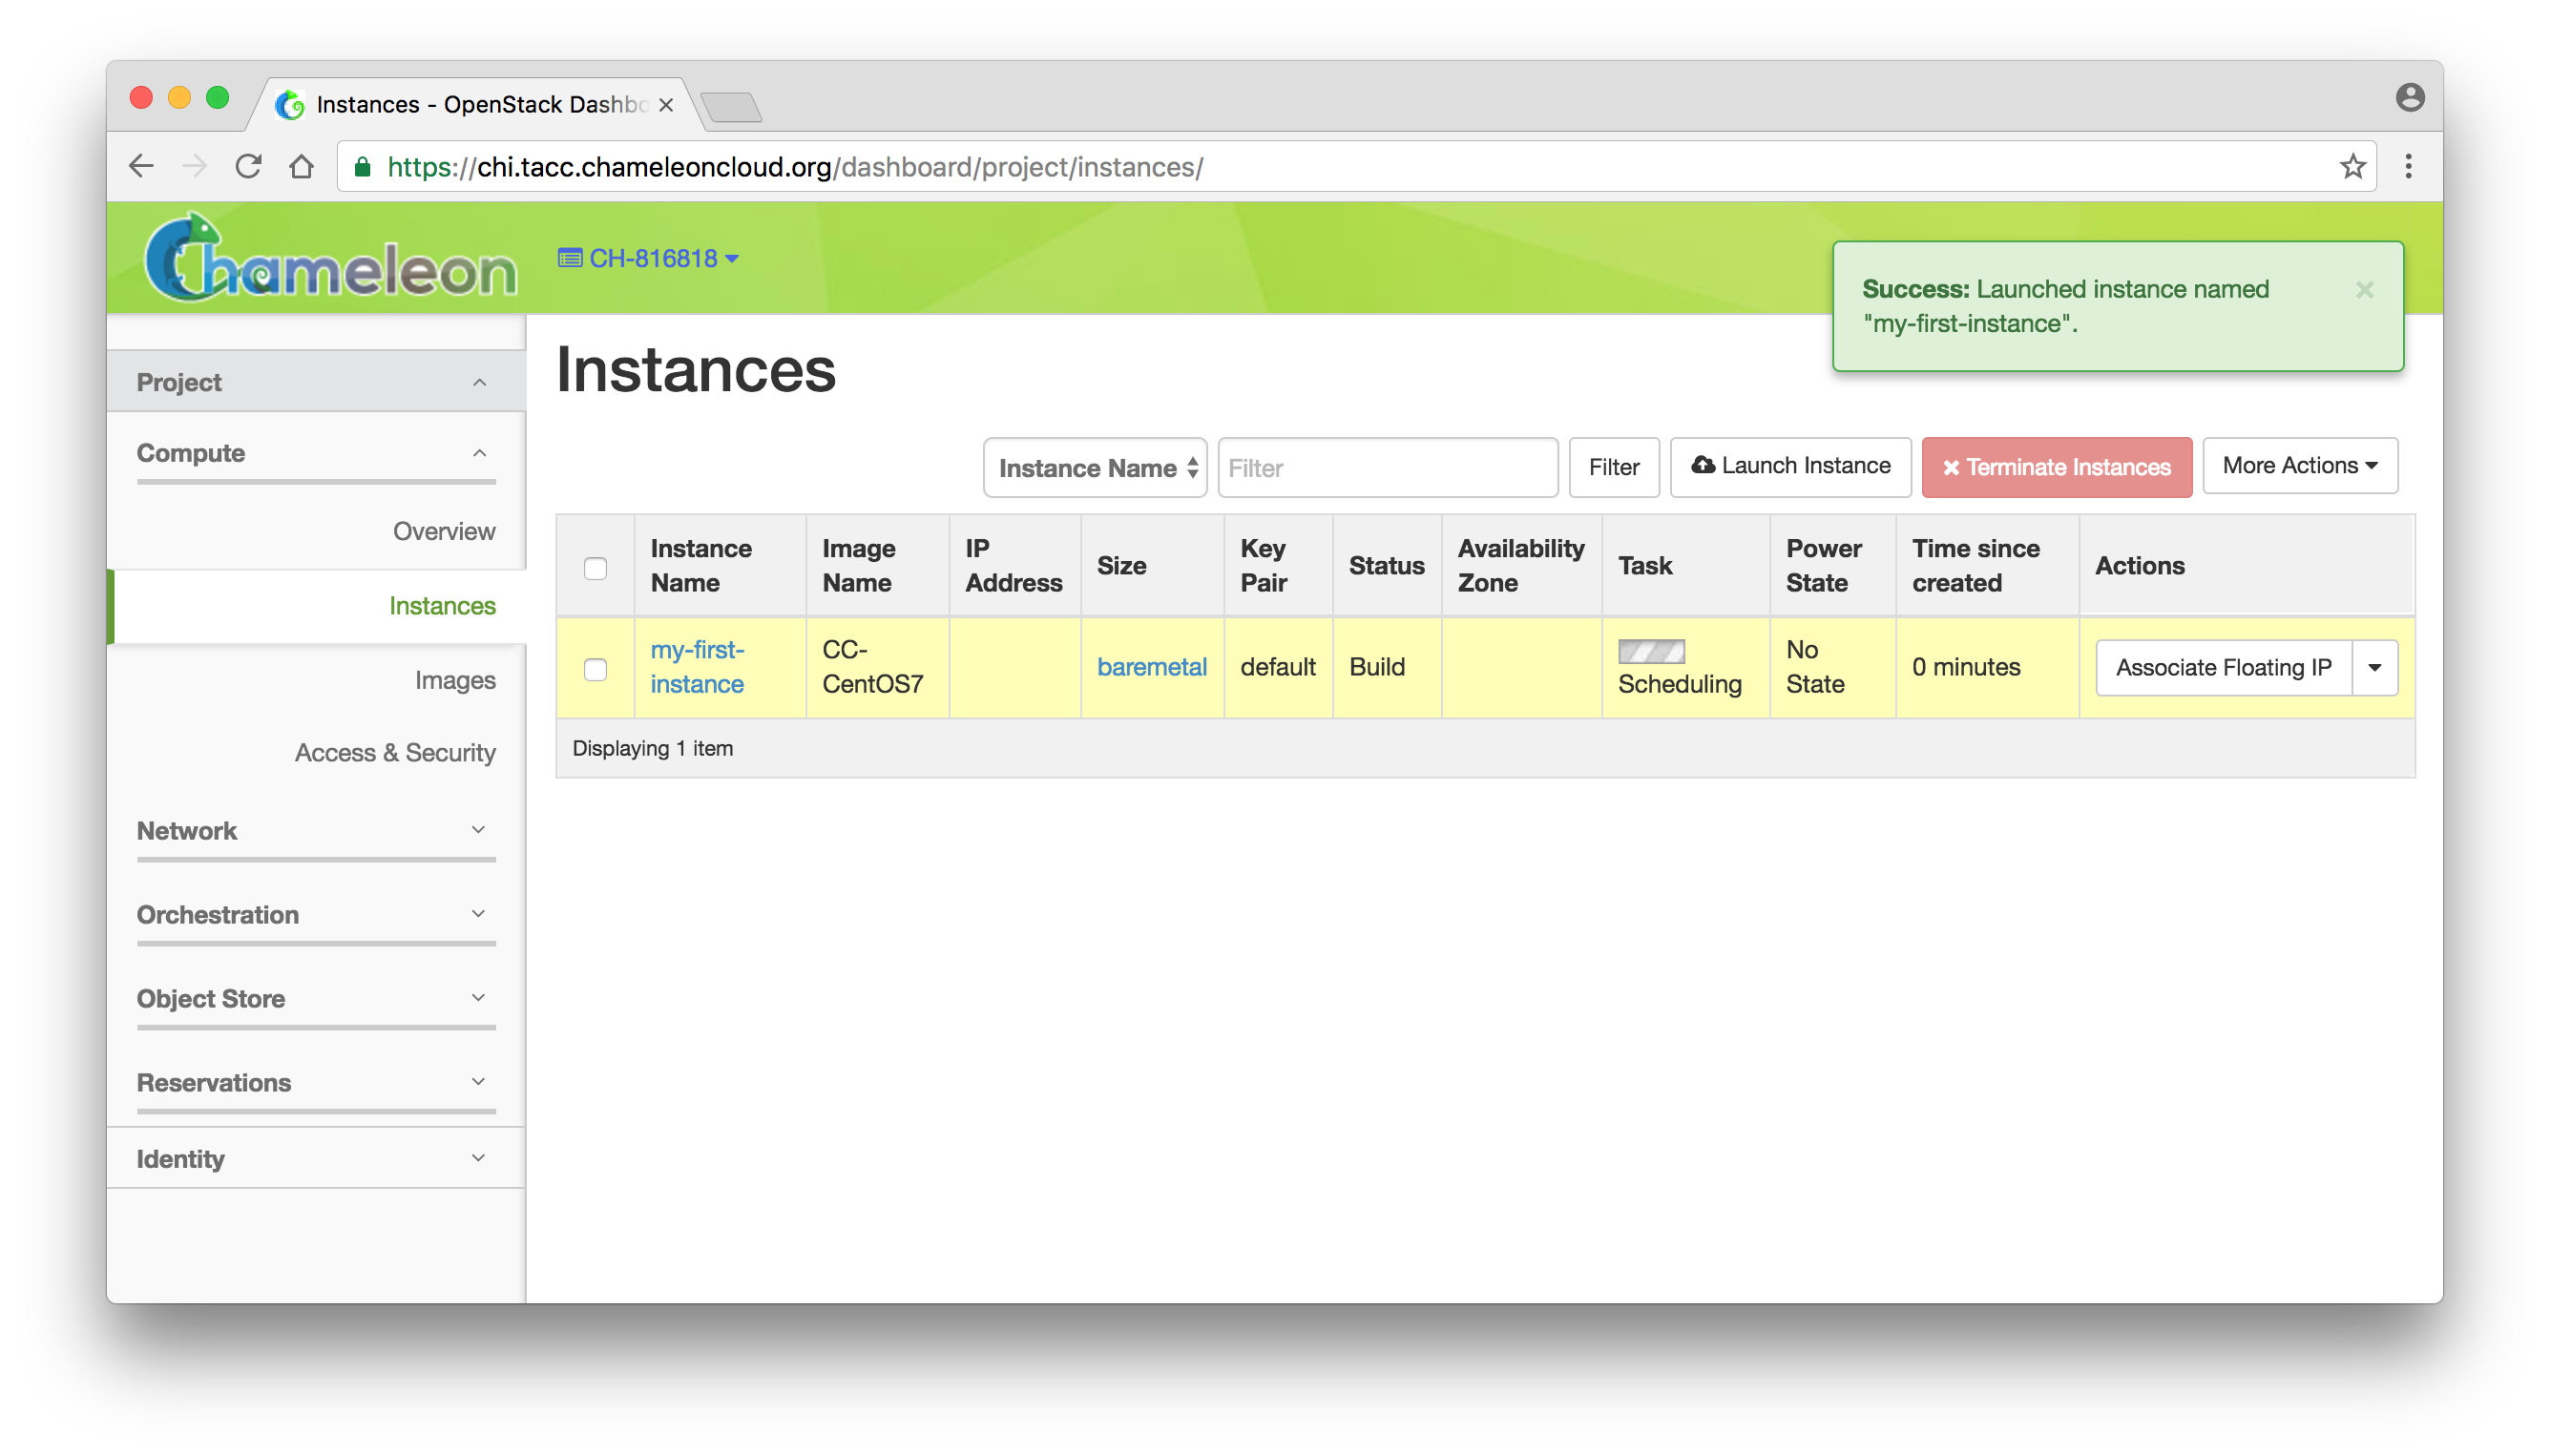
\includegraphics[width=\columnwidth]{images/chameleon/Screen-Shot-2016-10-26-at-15-53-31.png}

After a few minutes the instance should become in Active status and the
Power State should be Running.

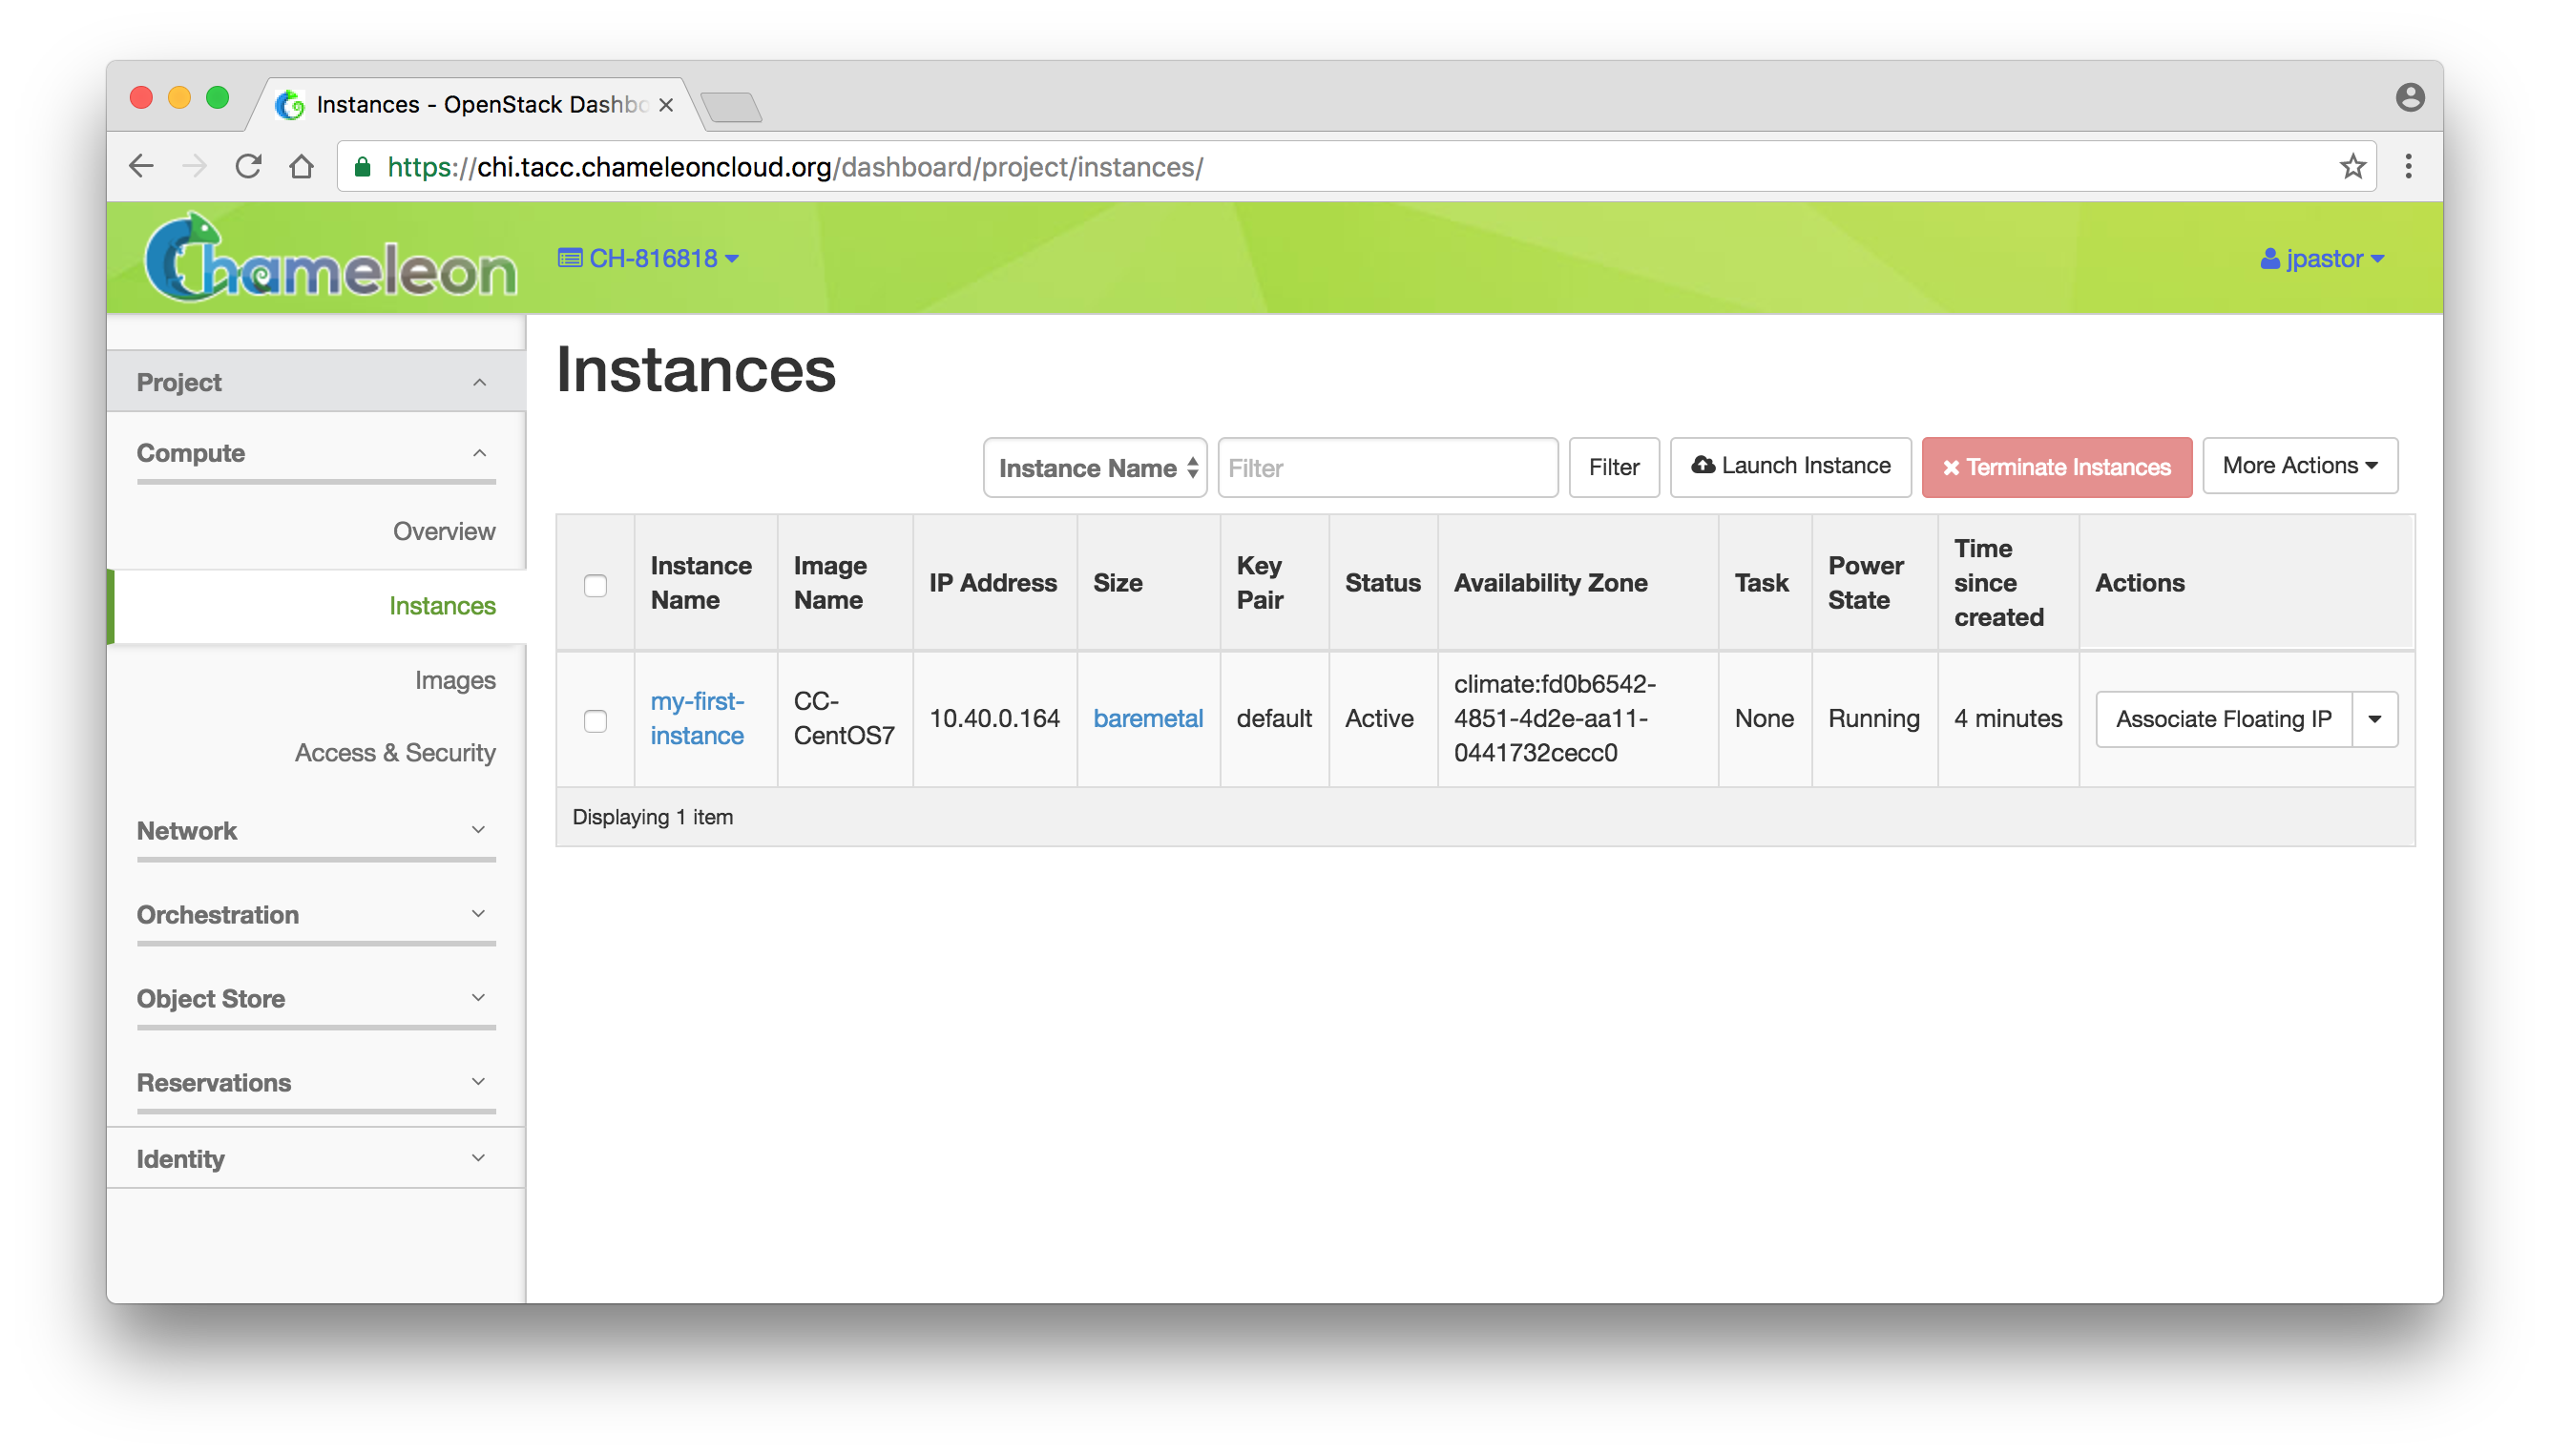
\includegraphics[width=\columnwidth]{images/chameleon/Screen-Shot-2016-10-26-at-16-22-38.png}

At this point the instance might still be booting: it might take a
minute or two to actually be accessible on the network and accept SSH
connections.~In the meantime, you can attach a floating IP to the
instance. Click on the~``Associate Floating IP'' button.~You should get
a screen like the one below:

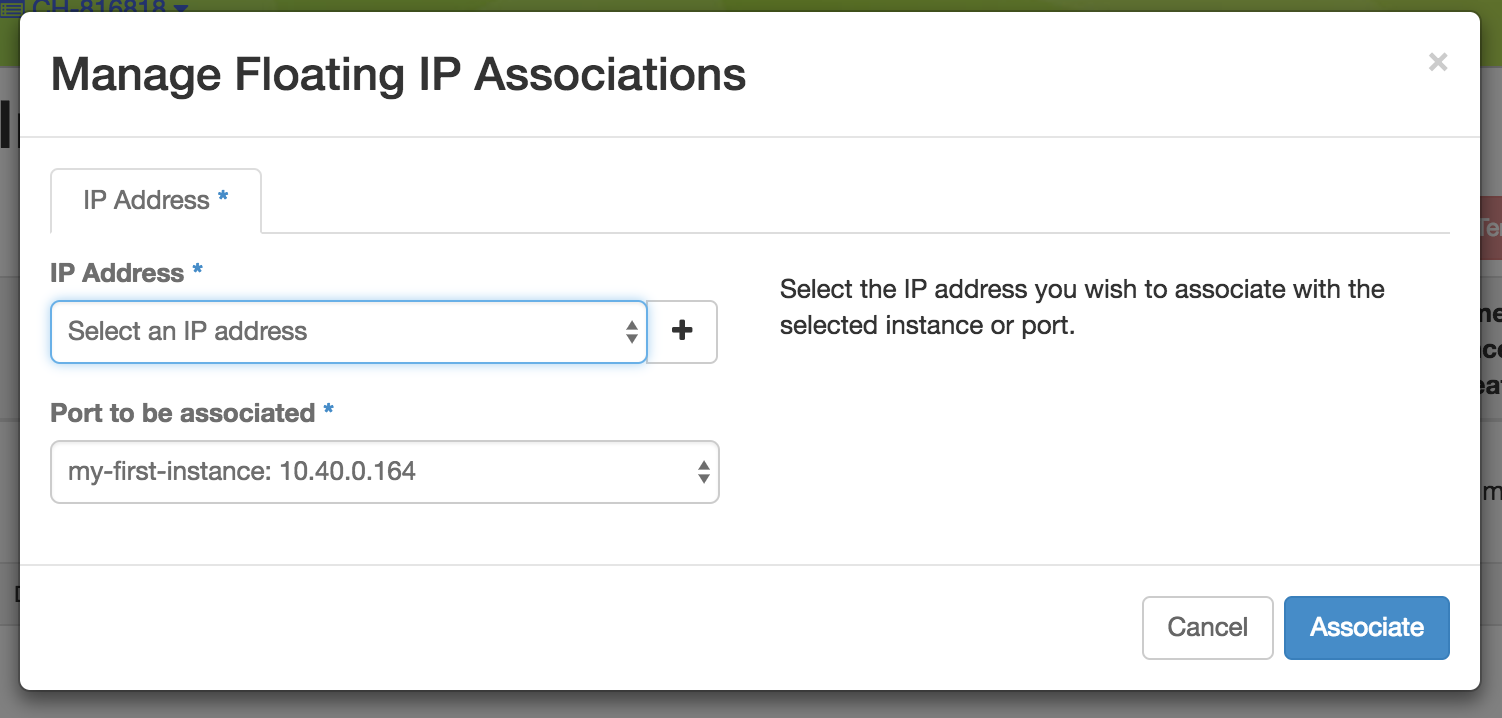
\includegraphics[width=\columnwidth]{images/chameleon/Screen-Shot-2016-10-26-at-16-25-04.png}

If there are no unused floating IP already allocated to your project,
click on the + button. In the window that opens, select the ext-net pool
if not already selected by default and click on the blue Allocate IP
button.

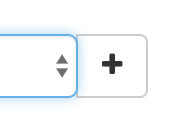
\includegraphics[width=\columnwidth]{images/chameleon/Screen-Shot-2016-10-26-at-16-33-45-W05kOLQ.png}

You will be returned to the previous window. The correct value for
``Port to be associated'' should already be selected, so you only have
to click on ``Associate''.

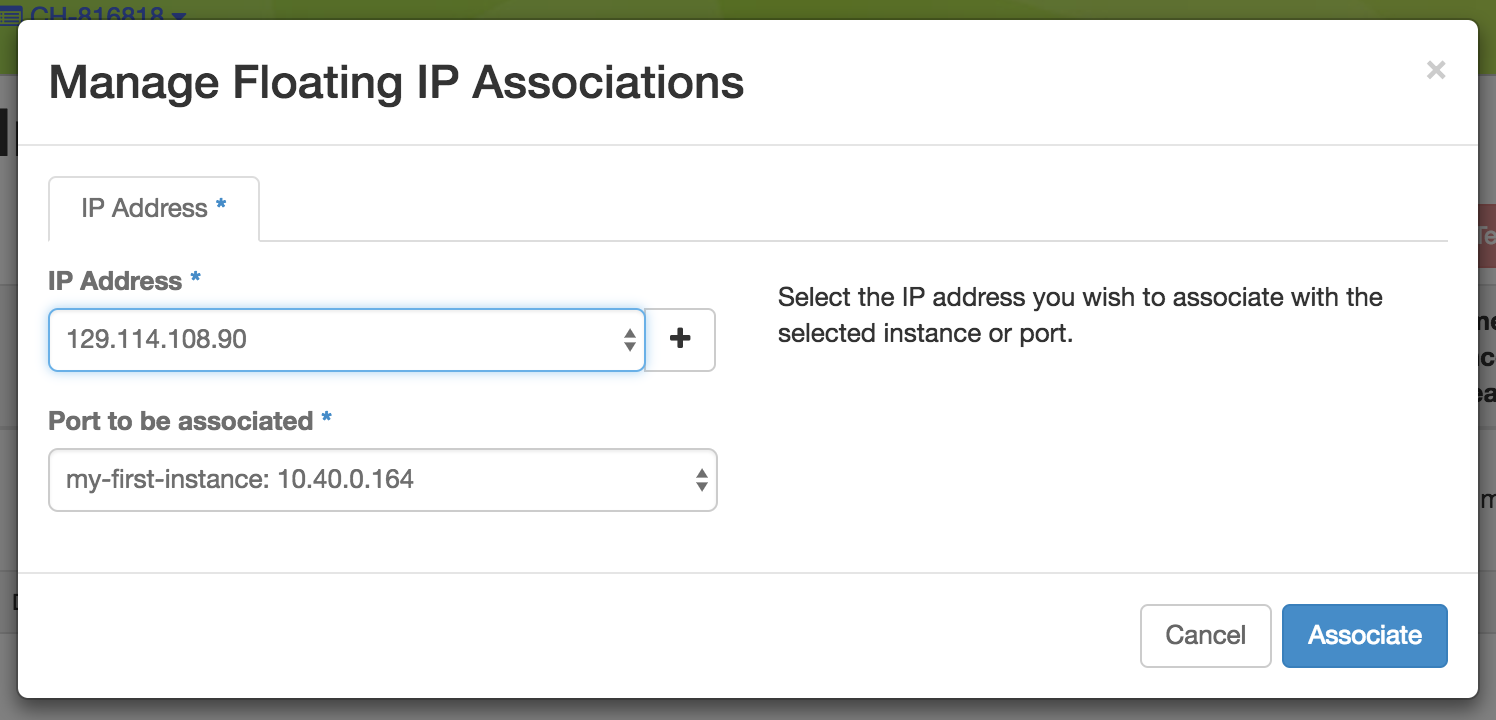
\includegraphics[width=\columnwidth]{images/chameleon/Screen-Shot-2016-10-26-at-16-25-10.png}

This should send you back to the instance list, where you can see the
floating IP attached to the instance (you may need to refresh your
browser to see the floating IP).

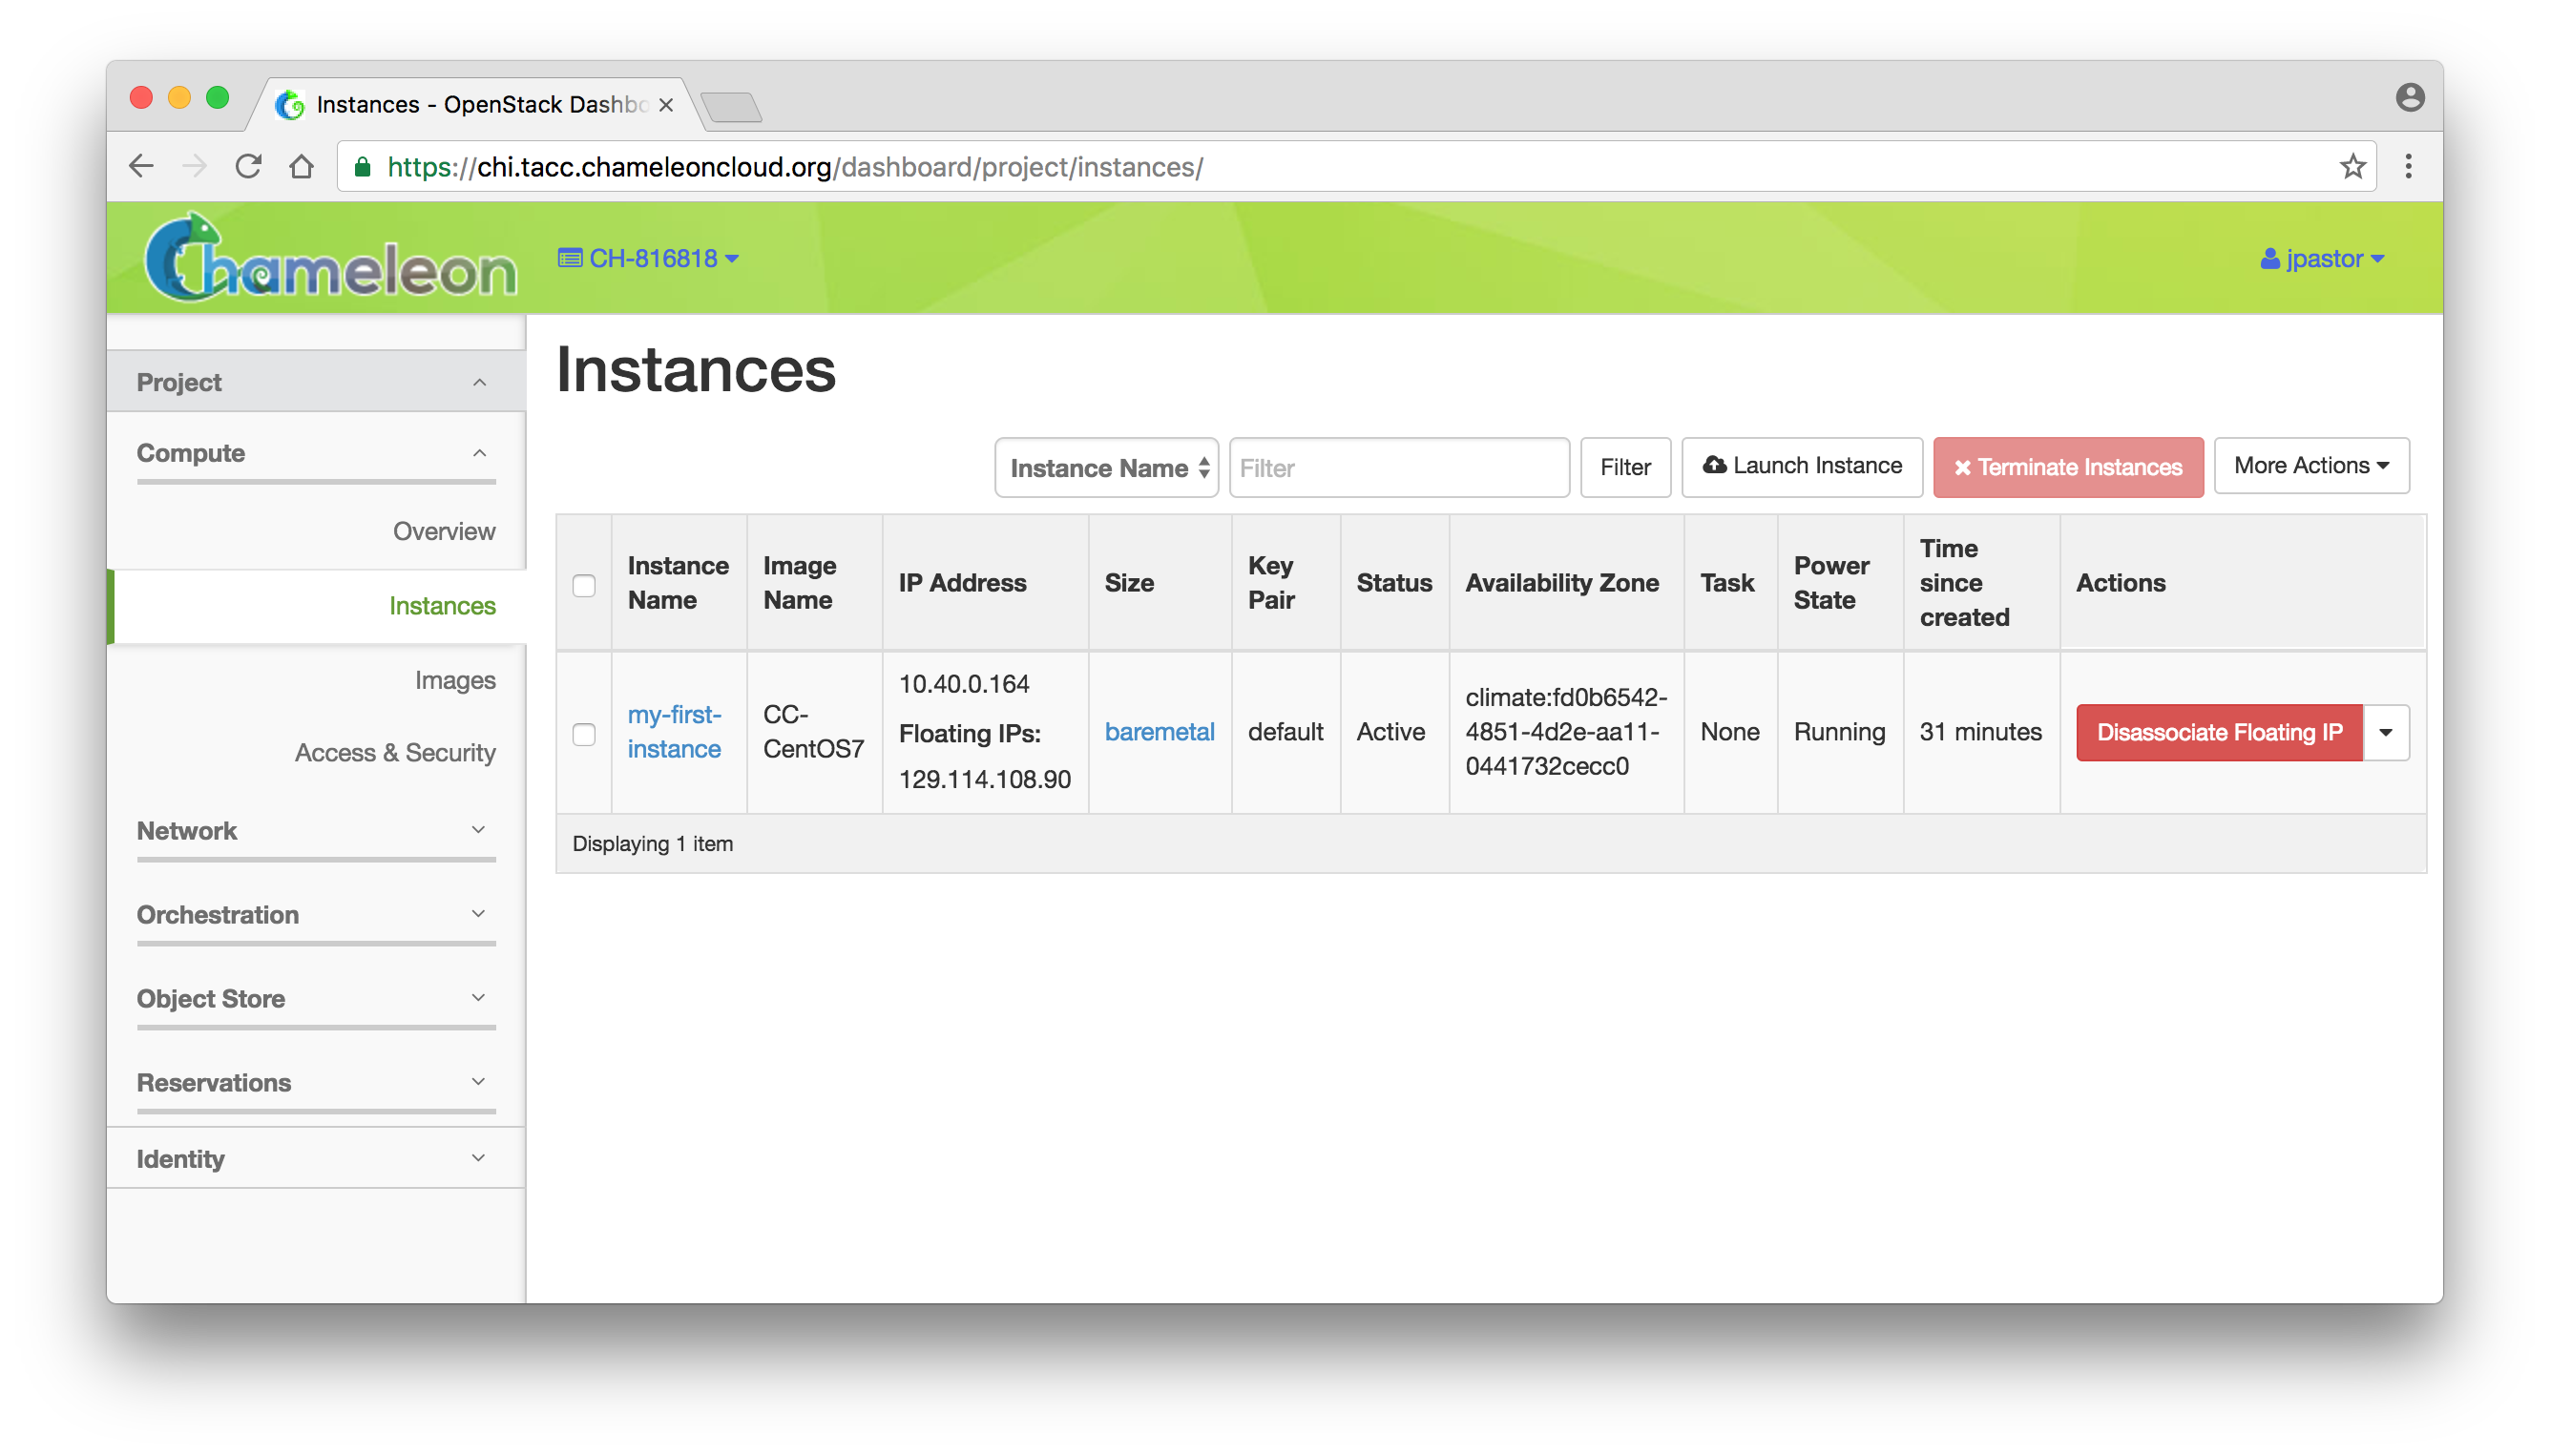
\includegraphics[width=\columnwidth]{images/chameleon/Screen-Shot-2016-10-26-at-16-26-54.png}

\section{Interact with resources}\label{interact-with-resources}

Now you should be able to connect to the instance via SSH using the cc
account. In a terminal, type ssh
cc@\textless{}floating\_ip\textgreater{}, in our example this would
be~\texttt{ssh\ cc@130.202.88.241}

SSH will probably tell you:

\begin{verbatim}
The authenticity of host \textquotesingle{}130.202.88.241
(130.202.88.241) can't be established. RSA key fingerprint 
is 5b:ca:f0:63:6f:22:c6:96:9f:c0:4a:d8:5e:dd:fd:eb. 
Are you sure you want to continue connecting (yes/no)?

\end{verbatim}

Type yes and press Enter. You should arrive to a prompt like this one:

\texttt{{[}cc@my-first-instance\ \textasciitilde{}{]}\$}

If you notice SSH errors such as connection refused, password requests,
or failures to accept your key, it is likely that the physical node is
still going through the boot process. In that case, please wait before
retrying. Also make sure that you use the~\textbf{cc}~account. If after
10 minutes you still cannot connect to the machine,
please~\href{https://www.chameleoncloud.org/user/help/}{open a ticket
with our help desk}.

You can now check whether the resource matches its known description in
the resource registry. For this, simply
run:~\texttt{sudo\ cc-checks\ -v}

{\centering 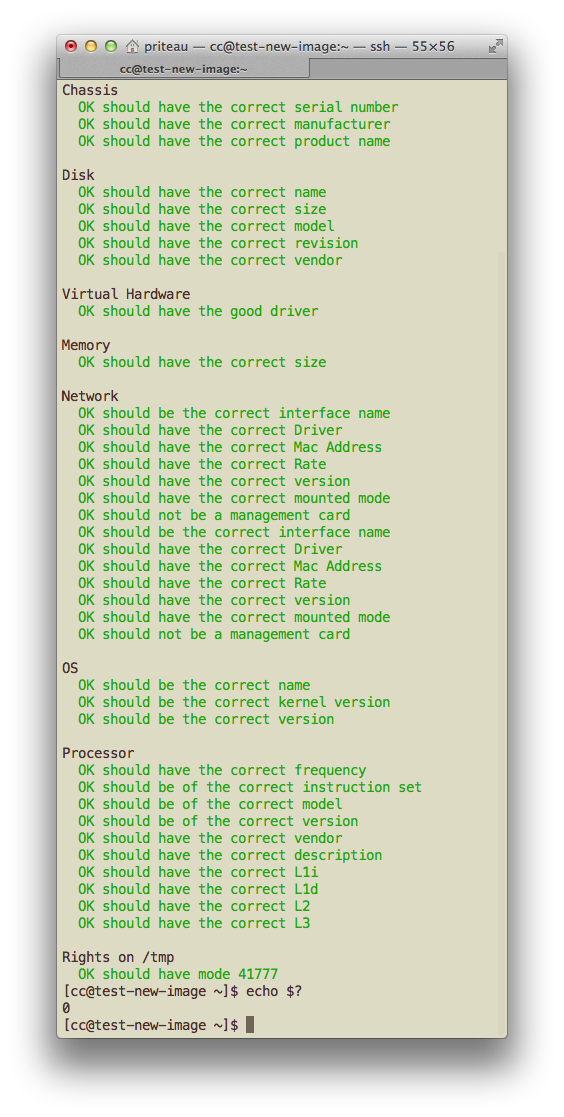
\includegraphics[width=0.5\columnwidth]{images/chameleon/cc-checks.png}}

The cc-checks program prints the result of each check in green if it is
successful and~red if it failed.

You can now run your experiment directly on the machine via SSH. You can
run commands with root privileges by prefixing them with~\texttt{sudo}.
To completely~switch~user and become root, use
the~\texttt{sudo\ su\ -\ root}~command.

\subsection{\texorpdfstring{{Snapshot an
instance}}{Snapshot an instance}}\label{snapshot-an-instance}

All instances in Chameleon, whether KVM or bare-metal, are running off
disk images. The content of these disk images can be snapshotted at any
point in time, which allows you to save your work and launch new
instances from updated images later.

While OpenStack KVM has built-in support for snapshotting in the Horizon
web interface and via the command line, bare-metal instances require a
more complex process. To make this process easier,{ we developed the
\href{https://github.com/ChameleonCloud/ChameleonSnapshotting}{cc-snapshot}
tool, which implements snapshotting a bare-metal instance from command
line and uploads it to Glance, so that it can be immediately used to
boot a new bare-metal instance. The snapshot images created with this
tool are whole disk images.}

{For ease of use, \emph{cc-snapshot} has been installed in all the
appliances supported by the Chameleon project. If you would like to use
it in a different setting, it can be downloaded and installed from the
\href{https://github.com/ChameleonCloud/ChameleonSnapshotting}{github
repository}.}

{Once cc-snapshot is installed, to make a snapshot of a bare-metal
instance, run the following command from inside the instance:}

{\texttt{sudo\ cc-snapshot\ \textless{}snapshot\_name\textgreater{}}}

{You can verify that it has been uploaded to Glance by running the
following command:}

{\texttt{glance\ image-list}}

{If you prefer to use a series of standard Unix commands, or are
generally interested in more detail about image management, please refer
to our
\href{https://www.chameleoncloud.org/docs/user-guides/ironic/\#snapshotting_an_instance}{image
management guide}.}

\section{Use FPGAs}\label{use-fpgas}

Consult the
\href{https://www.chameleoncloud.org/docs/bare-metal-user-guide/fpga/}{dedicated
page}~if you would like to use the FPGAs available on Chameleon.

\section{Next Step}\label{next-step}

Now that you have created some resources, it is time to interact with
them! You will find instructions to the next step by visiting the
following link:

\begin{itemize}
\tightlist
\item
  \href{https://www.chameleoncloud.org/monitor-and-collect/}{Monitor
  resources and collect results}
\end{itemize}


\FILENAME

\chapter{HEAT}\label{complex-appliances}

\section{What are complex~appliances?}\label{what-are-complexappliances}

Deploying an MPI cluster, an OpenStack installation, or any other type
of cluster in which nodes can take on multiple roles can be complex: you
have to provision potentially hundreds of nodes, configure them to take
on various roles, and make them share information that is generated or
assigned only at deployment time, such as hostnames, IP addresses, or
security keys. When you want to run a different experiment later you
have to redo all this work. When you want to reproduce the experiment,
or allow somebody else to reproduce it, you have to take very precise
notes and pay great attention to their execution.

To help solve this problem and facilitate reproducibility and sharing,
the Chameleon team configured a tool that allows you to deploy complex
clusters with ``one click''. This tool requires not just a simple image
(i.e., appliance) but also a document, called a template, that contains
the information needed to orchestrate the deployment and configuration
of such clusters. We call this image + template combination
complex~appliance because it consists of more than just the image (i.e.,
appliance).

\section{How are complex appliances
supported?}\label{how-are-complex-appliances-supported}

In a nutshell, complex appliances allow you to specify not only what
image you want to deploy but also on how many nodes you want to deploy
that image, what roles the deployed instances should boot into (such as
e.g., head node and worker node in a cluster), what information from a
specific instance should be passed to another instance in that complex
appliance, and what scripts should be executed on boot so that this
information is properly used for configuring the ``one click'' cluster.
For example, a Network File System (NFS) appliance that we will use as
an example in this guide, might specify deployment on three nodes, out
of which one will be configured as head node and others as worker nodes,
the information passed between the images will be hostname of the head
node, and the scripts executed on the worker nodes on boot will put that
hostname in the fstab file. As you can tell from this description,
images used for complex appliances are typically configured such that
they can be booted into any role required on the one-click cluster we
are booting; in this case the image will have both the software for NFS
server node and client~node.

Since complex appliances in Chameleon are currently implemented using
the \href{https://wiki.openstack.org/wiki/Heat}{OpenStack Heat}
orchestration service, we will be using OpenStack terminology and
features to work with them. The templates described above are YAML files
using the
\href{http://docs.openstack.org/developer/heat/template_guide/hot_spec.html}{Heat
Orchestration Template (HOT) format} (Heat also supports the AWS
CloudFormation template format, but this is not covered here). A
deployed complex appliance is referred to as a ``stack'' -- just as a
deployed single appliance is typically referred to as an ``instance''.
This guide will tell you all you need to know in order to use and
configure complex appliances on Chameleon; if you would like to know
more about Heat, please refer to its
\href{http://docs.openstack.org/developer/heat/}{official
documentation}.

\section{Where can I find Chameleon complex
appliances?}\label{where-can-i-find-chameleon-complex-appliances}

Our \href{https://www.chameleoncloud.org/appliances/}{Appliance Catalog}
has several complex appliances for popular technologies that people want
to deploy such as OpenStack or MPI or even more advanced deployments
such as efficient SR-IOV enabled MPI in KVM virtual machines. We also
provide common building blocks for cluster architectures, such as an NFS
share. Complex appliances are identified by a badge in their top-right
corner representing a group of machines, as shown in the screenshot:

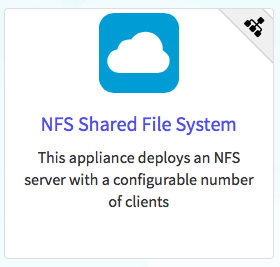
\includegraphics[width=0.5\columnwidth]{images/chameleon/NFS.png}

\section{How do I deploy a complex
appliance?}\label{how-do-i-deploy-a-complex-appliance}

We will explain how to launch a complex appliance based on our
\href{https://www.chameleoncloud.org/appliances/25/}{NFS share
appliance}. To launch a complex appliance, you only need to follow these
steps:

\begin{enumerate}
\item
  Create a lease: use the OpenStack web interface (choose between CHI@UC
  or CHI@TACC) to create a lease. To launch our NFS appliance, reserve
  at least three compute nodes (the strict minimum is two nodes but we
  will use three in this example and later ones).
\item
  Go to the \href{https://www.chameleoncloud.org/appliances/}{Appliance
  Catalog} and identify the appliance you want to launch. In our case
  you can go straight to the
  \href{https://www.chameleoncloud.org/appliances/25/}{NFS
  share~appliance}; click on it to open its details page. You will see a
  ``Launch'' button and a ``Get Template'' button. Follow the ``Get
  Template'' link and copy its url to the clipboard --~you will need it
  in the following steps.
\item
  Click on the ``Launch Complex Appliance at CHI@TACC'' or ``Launch
  Complex Appliance at CHI@UC'' button depending on where your
  reservation was created.
\end{enumerate}

This will take you to the Stacks page within the Orchestration menu.
This page will show the current list of stacks, with controls to manage
them and create new ones. Since we haven't launched any yet, this list
will be empty for now.

We will now create a new stack, which corresponds to the launch of a
template. Click on Launch Stack on the top right. A window will pop up
like below:

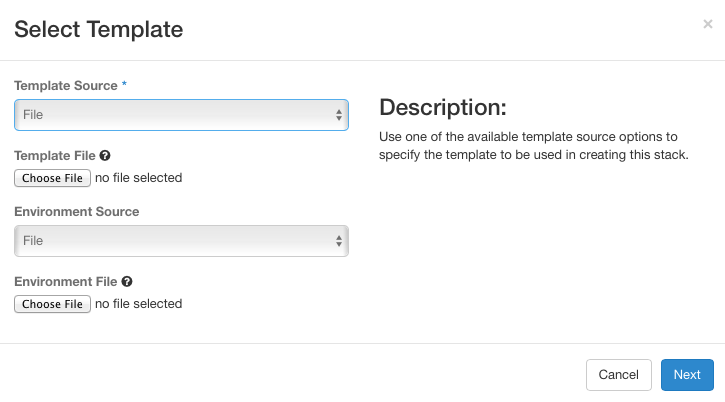
\includegraphics[width=\columnwidth]{images/chameleon/Launch-Stack.png}

We will deploy the NFS appliance described earlier; it will consist of a
server node and two client nodes. Change the template source field to
URL, and paste the URL of the
\href{https://www.chameleoncloud.org/appliances/api/appliances/25/template}{NFS
share~template} (if you don't have it in your clipboard anymore you will
need to go back to the appliance and get it by clicking on ``Get
template'' again).

Don't change the environment source settings, and click ``Next''.

The next screen allows your to enter input values to your Heat template.
Choose a name for your stack (e.g. my-nfs-cluster). Ignore the
``Creation Timeout'' and ``Rollback On Failure'' settings. You also need
to enter your Chameleon password. Then, you need to select a value for
the three parameters of the template: for key\_name, choose your SSH key
pair (this key pair will authorize access on each deployed instances,
both server and client). For nfs\_client\_count, change the default
value of 1 to 2. For reservation\_id, choose your reservation created
earlier. Finally, click ``Launch''.

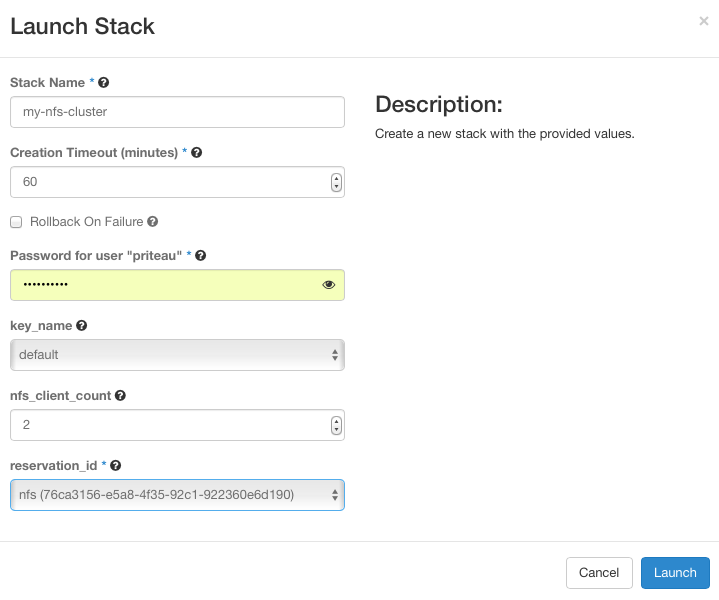
\includegraphics[width=\columnwidth]{images/chameleon/Launch-NFS-Stack.png}

Your stack should be in status ``Create In Progress'' for several
minutes while it first launches the NFS server instance, followed by the
NFS client instances.

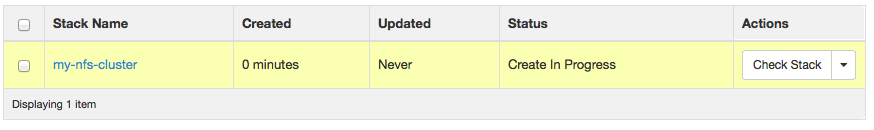
\includegraphics[width=\columnwidth]{images/chameleon/Create-In-Progress_zPgOjo4.png}

It will then move to the status ``Create Complete''.

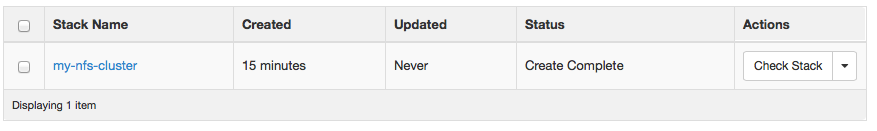
\includegraphics[width=\columnwidth]{images/chameleon/Create-Complete_XkoWhlj.png}

You can click on the stack name to get more details, including a
visualization of the deployed resources, as pictured below. The single
machine inside a circle represents the NFS server instance. The rack of
machine represents the group of NFS client instances (in this case, a
group composed of two instances). The server's floating IP (the public
IP assigned to a resource) is represented by an IP in a circle; an~IP in
a circle is also used to represent the association of the IP with~the
NFS server instance (not the greatest idea to use the same symbol for
both the IP and the association -- we agree but can't do much about it
at the moment). Blow off some steam by dragging the visualization across
the screen, it can be rather fun!

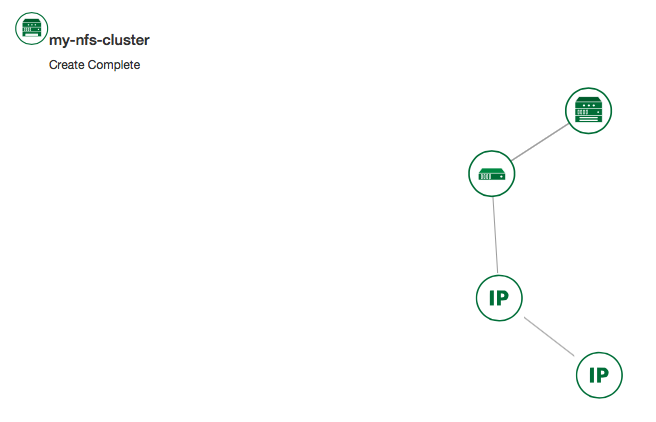
\includegraphics[width=\columnwidth]{images/chameleon/Stack-visualization.png}

You can now ssh to the server using the floating IP just as you do with
regular instances (use the cc account). The client does not have a
floating IP attached to it (as per the visualization above) but you can
connect to it via the server node with the client's private IP (connect
to the server with \texttt{ssh\ -A}~to enable the SSH agent forwarding
after loading your key to your SSH agent
with~\texttt{ssh-add\ \textless{}path-to-your-key\textgreater{}}).

You can find out the information about the IPs and other things if you
click the ``Overview'' tab and look in the ``Outputs'' section. Under
the ``Resources'' tab you will see the resources described above (the
server, clients, server's public/floating IP, and its the association)
and information about them. In the ``Events'' tab you will see
information about the history of the deployment so far. In Template you
will see the template that was used to deploy this stack.

\section{What is inside a Heat
template?}\label{what-is-inside-a-heat-template}

The NFS share appliance deploys:

\begin{itemize}
\item
  an NFS server instance, that exports the directory /exports/example to
  any instance running on Chameleon bare-metal,
\item
  one or several NFS client instances, which configure /etc/fstab to
  mount this NFS share to /mnt (and can subsequently read from and write
  to it).
\end{itemize}

This template is reproduced further below, and includes inline comments
starting with the \# character. There are three main sections:

\begin{itemize}
\item
  resources,
\item
  parameters,
\item
  outputs.
\end{itemize}

The resources section is the most important part of the template: it
defines which OpenStack resources to create and configure. Inside this
section you can see four resources defined:

\begin{itemize}
\item
  nfs\_server\_floating\_ip
\item
  nfs\_server~
\item
  nfs\_server\_ip\_association
\item
  nfs\_clients
\end{itemize}

The first resource, nfs\_server\_floating\_ip, creates a floating IP on
the ext-net public network. It is not attached to any instance yet.

The second resource, nfs\_server, creates the NFS server instance (an
instance is defined with the type \texttt{OS::Nova::Server} in Heat). It
is a bare-metal instance (\texttt{flavor:\ baremetal}) using the
CC-CentOS7 image and connected to the private network named sharednet1.
We set the keypair to use the value of the parameter defined earlier,
using the \texttt{get\_param} function. Similarly, the reservation to
use is passed to the scheduler. Finally, a user-data script is given to
the instance, which configures it as an NFS server exporting
/exports/example to Chameleon instances.

The nfs\_server\_ip\_association resource associates the floating IP
created earlier with the NFS server instance.

Finally, the nfs\_clients resource defines a resource group containing
instance configured to be NFS clients and mount the directory exported
by the NFS server defined earlier. The IP of the NFS server is gathered
using the \texttt{get\_attr} function, and placed into user-data using
the \texttt{str\_replace} function.

Parameters all have the same data structure: each one has a name
(\texttt{key\_name} or \texttt{reservation\_id} in this case), a data
type (number or string), a comment field called description, optionally
a default value, and a list of constraints (in this case only one per
parameter). Constraints tell Heat to match a parameter to a specific
type of OpenStack resource. Complex appliances on Chameleon require
users to customize at least the key pair name and reservation ID, and
will generally provide additional parameters to customize other
properties of the cluster, such as its size, as in this example.

Outputs are declared similarly to parameters: they each have a name, an
optional~description, and a value. They allow to return information from
the~stack to the user.

\begin{footnotesize}
\begin{verbatim}
# This describes what is deployed by this template.
description: NFS server and clients deployed with Heat on Chameleon

# This defines the minimum Heat version required by this template.
heat_template_version: 2015-10-15

# The resources section defines what OpenStack resources are to be deployed and
# how they should be configured.
resources:
  nfs_server_floating_ip:
    type: OS::Nova::FloatingIP
    properties:
      pool: ext-net

  nfs_server:
    type: OS::Nova::Server
    properties:
      flavor: baremetal
      image: CC-CentOS7
      key_name: { get_param: key_name }
      networks:
         - network: sharednet1
      scheduler_hints: { reservation: { get_param: reservation_id } }
      user_data: |
        #!/bin/bash
        yum install -y nfs-utils
        mkdir -p /exports/example
        chown -R cc:cc /exports
        echo '/exports/example 10.140.80.0/22(rw,async) 10.40.0.0/23(rw,async)' >> /etc/exports
        systemctl enable rpcbind && systemctl start rpcbind
        systemctl enable nfs-server && systemctl start nfs-server

  nfs_server_ip_association:
    type: OS::Nova::FloatingIPAssociation
    properties:
      floating_ip: { get_resource: nfs_server_floating_ip }
      server_id: { get_resource: nfs_server }

  nfs_clients:
    type: OS::Heat::ResourceGroup
    properties:
      count: { get_param: nfs_client_count }
      resource_def:
        type: OS::Nova::Server
        properties:
          flavor: baremetal
          image: CC-CentOS7
          key_name: { get_param: key_name }
          networks:
             - network: sharednet1
          scheduler_hints: { reservation: { get_param: reservation_id } }
          user_data:
            str_replace:
              template: |
                #!/bin/bash
                yum install -y nfs-utils
                echo "$nfs_server_ip:/exports/example    /mnt/    nfs" > /etc/fstab
                mount -a
              params:
                $nfs_server_ip: { get_attr: [nfs_server, first_address] }

# The parameters section gathers configuration from the user.
parameters:
  nfs_client_count:
    type: number
    description: Number of NFS client instances
    default: 1
    constraints:
      - range: { min: 1 }
        description: There must be at least one client.
  key_name:
    type: string
    description: Name of a KeyPair to enable SSH access to the instance
    default: default
    constraints:
    - custom_constraint: nova.keypair
  reservation_id:
    type: string
    description: ID of the Blazar reservation to use for launching instances.
    constraints:
    - custom_constraint: blazar.reservation

outputs:
  server_ip:
    description: Public IP address of the NFS server
    value: { get_attr: [nfs_server_floating_ip, ip] }
  client_ips:
    description: Private IP addresses of the NFS clients
    value: { get_attr: [nfs_clients, first_address] }
\end{verbatim}
\end{footnotesize}

\section{Customizing an existing
template}\label{customizing-an-existing-template}

Customizing an existing template is a good way to start developing your
own. We will use a simpler template than the previous example to start
with: it is
the~\href{https://www.chameleoncloud.org/appliances/26/}{Hello World
complex appliance}.

First, delete the stack you launched, because we will need all three
nodes to be free. To do this, go back to the Project \textgreater{}
Orchestration \textgreater{} Stacks page, select your stack, and then
click on the red ``Delete Stacks'' button. You will be asked to confirm,
so click on the blue~``Delete Stacks'' button.

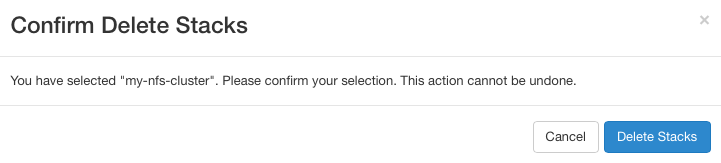
\includegraphics[width=\columnwidth]{images/chameleon/Delete-Stacks.png}

The template for the
\href{https://www.chameleoncloud.org/appliances/26/}{Hello World complex
appliance}~is~reproduced below. It is similar to the NFS share
appliance, except that it deploys only a single client. You can see that
it has four resources defined:

\begin{itemize}
\item
  nfs\_server\_floating\_ip
\item
  nfs\_server
\item
  nfs\_server\_ip\_association
\item
  nfs\_client
\end{itemize}

The nfs\_client instance mounts the NFS directory shared by the
nfs\_server instance, just like in our earlier example.

\begin{footnotesize}
\begin{verbatim}
# This describes what is deployed by this template.
description: NFS server and client deployed with Heat on Chameleon

# This defines the minimum Heat version required by this template.
heat_template_version: 2015-10-15

# The resources section defines what OpenStack resources are to be deployed and
# how they should be configured.
resources:
  nfs_server_floating_ip:
    type: OS::Nova::FloatingIP
    properties:
      pool: ext-net

  nfs_server:
    type: OS::Nova::Server
    properties:
      flavor: baremetal
      image: CC-CentOS7
      key_name: { get_param: key_name }
      networks:
         - network: sharednet1
      scheduler_hints: { reservation: { get_param: reservation_id } }
      user_data: |
        #!/bin/bash
        yum install -y nfs-utils
        mkdir -p /exports/example
        chown -R cc:cc /exports
        echo '/exports/example 10.140.80.0/22(rw,async) 10.40.0.0/23(rw,async)' >> /etc/exports
        systemctl enable rpcbind && systemctl start rpcbind
        systemctl enable nfs-server && systemctl start nfs-server

  nfs_server_ip_association:
    type: OS::Nova::FloatingIPAssociation
    properties:
      floating_ip: { get_resource: nfs_server_floating_ip }
      server_id: { get_resource: nfs_server }

  nfs_client:
    type: OS::Nova::Server
    properties:
      flavor: baremetal
      image: CC-CentOS7
      key_name: { get_param: key_name }
      networks:
         - network: sharednet1
      scheduler_hints: { reservation: { get_param: reservation_id } }
      user_data:
        str_replace:
          template: |
            #!/bin/bash
            yum install -y nfs-utils
            echo "$nfs_server_ip:/exports/example    /mnt/    nfs" > /etc/fstab
            mount -a
          params:
            $nfs_server_ip: { get_attr: [nfs_server, first_address] }

# The parameters section gathers configuration from the user.
parameters:
  key_name:
    type: string
    description: Name of a KeyPair to enable SSH access to the instance
    default: default
    constraints:
    - custom_constraint: nova.keypair
  reservation_id:
    type: string
    description: ID of the Blazar reservation to use for launching instances.
    constraints:
    - custom_constraint: blazar.reservation
\end{verbatim}
\end{footnotesize}

Download this template from the
\href{https://www.chameleoncloud.org/appliances/26/}{Hello World complex
appliance details page} to your local machine, and open it in your
favorite text editor.

We will customize~the template to add a second NFS~client by creating a
new resource called another\_nfs\_client. Add the following text to your
template inside the resources section.~Make sure to respect the level of
indentation, which is important in YAML.

\begin{footnotesize}
\begin{verbatim}
  another_nfs_client:
    type: OS::Nova::Server
    properties:
      flavor: baremetal
      image: CC-CentOS7
      key_name: { get_param: key_name }
      networks:
         - network: sharednet1
      scheduler_hints: { reservation: { get_param: reservation_id } }
      user_data:
        str_replace:
          template: |
            #!/bin/bash
            yum install -y nfs-utils
            echo "$nfs_server_ip:/exports/example    /mnt/    nfs" > /etc/fstab
            mount -a
          params:
            $nfs_server_ip: { get_attr: [nfs_server, first_address] }
\end{verbatim}
\end{footnotesize}

Now, launch a new~stack~with this~template. Since the customized
template is only on your computer and cannot be addressed by a URL, use
the ``Direct Input'' method instead and copy/paste the content of the
customized template.~The resulting topology view is shown below:~as you
can see, the two client instances are shown separately since each one is
defined as a separate resource in the template.

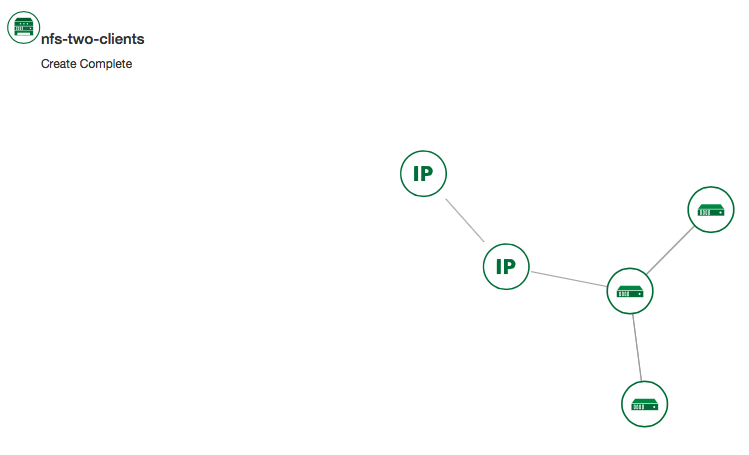
\includegraphics[width=\columnwidth]{images/chameleon/NFS-Two-Clients_lFGgizN.png}

You may have realized~already that while adding just one additional
client instance~was easy, launching more of them would require to copy /
paste blocks of YAML many times while ensuring that the total count is
correct. This would be easy to get wrong, especially when dealing with
tens or hundreds of instances.

So instead, we leverage another construct from Heat: resource groups.
Resource groups allow to define one kind of resource and request it to
be created any~number of times.

Remove the nfs\_client and another\_client resources from your
customized template, and replace them with the following:

\begin{footnotesize}
\begin{verbatim}
  nfs_clients:
    type: OS::Heat::ResourceGroup
    properties:
      count: 2
      resource_def:
        type: OS::Nova::Server
        properties:
          flavor: baremetal
          image: CC-CentOS7
          key_name: { get_param: key_name }
          networks:
             - network: sharednet1
          scheduler_hints: { reservation: { get_param: reservation_id } }
          user_data:
            str_replace:
              template: |
                #!/bin/bash
                yum install -y nfs-utils
                echo "$nfs_server_ip:/exports/example    /mnt/    nfs" > /etc/fstab
                mount -a
              params:
                $nfs_server_ip: { get_attr: [nfs_server, first_address] }
\end{verbatim}
\end{footnotesize}

A resource group is configured with a properties field, containing the
definition of the resource to launch (\texttt{resource\_def}) and the
number of resources to launch (\texttt{count}). Once launched, you will
notice that the topology view groups all client instances under a single
Resource Group icon. We use the same \texttt{resource\_def} than when
defining separate instances earlier.

Another way we can customize this template is by adding outputs to the
template. Outputs allow a Heat template to return data to the user. This
can be useful to return values like IP addresses or credentials that the
user must know to use the system.

We will create an output returning the floating IP address used by the
NFS server. We define an outputs section, and one output with the name
\texttt{server\_ip} and a description. The value of the output is
gathered using the \texttt{get\_attr} function which obtains the IP
address of the server instance.

\begin{footnotesize}
\begin{verbatim}
outputs:
  server_ip:
    description: Public IP address of the NFS server
    value: { get_attr: [nfs_server_floating_ip, ip] }
\end{verbatim}
\end{footnotesize}

You can get outputs in the ``Overview'' tab of the Stack~Details page.
If you want to use~the command line, install \texttt{python-heatclient}
and use~the \texttt{heat\ output-list} and \texttt{heat\ output-show}
commands, or get a full list in the information returned by
\texttt{heat\ stack-show}.

Multiple outputs can be defined in the outputs section. Each of them
needs to have a unique name. For example, we can add another output to
list the private IPs assigned to client instances:

\begin{footnotesize}
\begin{verbatim}
  client_ips:
    description: Private IP addresses of the NFS clients
    value: { get_attr: [nfs_clients, first_address] }
\end{verbatim}
\end{footnotesize}

The image below shows the resulting outputs as viewed from the web
interface. Of course IP addresses will be specific to each deployment.

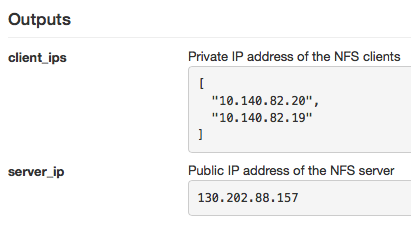
\includegraphics[width=0.5\columnwidth]{images/chameleon/Outputs.png}

Finally, we can add a new parameter to replace the hardcoded number of
client instances by a value passed to the template. Add the following
text to the parameters section:

\begin{footnotesize}
\begin{verbatim}
  nfs_client_count:
    type: number
    description: Number of NFS client instances
    default: 1
    constraints:
      - range: { min: 1 }
        description: There must be at least one client.
\end{verbatim}
\end{footnotesize}

Inside the resource group definition,
change~\texttt{count:\ 2}~to~\texttt{count:\ \{\ get\_param:\ nfs\_client\_count\ \}}~to
retrieve and use the parameter we just defined. When you launch this
template, you will see that an additional parameter allows you to define
the number of client instances, like in the NFS share~appliance.

At this stage, we have fully recreated the NFS share appliance starting
from the Hello World one! The next section will explain how to write a
new template from scratch.

\section{Writing a new template}\label{writing-a-new-template}

You may want to write a whole new template, rather than customizing an
existing one. Each template should follow the same layout and be
composed of the following sections:

\begin{itemize}
\item
  Heat template version
\item
  Description
\item
  Resources
\item
  Parameters
\item
  Outputs
\end{itemize}

\subsection{Heat template version}\label{heat-template-version}

Each Heat template has to include the heat\_template\_version key with a
valid version of HOT (Heat Orchestration Template). Chameleon bare-metal
supports any HOT version up to 2015-10-15, which corresponds to
OpenStack Liberty. The
\href{http://docs.openstack.org/developer/heat/template_guide/hot_spec.html\#hot-spec-template-version}{Heat
documentation}~lists~all available~versions and their features.~We
recommended that you always use the latest supported~version to have
access to all supported features:

\texttt{heat\_template\_version:\ 2015-10-15}

\subsection{Description}\label{description}

While not mandatory, it is good practice to describe what ~is deployed
and configured by your template. It can be on a single line:

\begin{footnotesize}
\begin{verbatim}
description: This describes what this Heat template deploys on Chameleon.
\end{verbatim}
\end{footnotesize}

If a longer description is needed, you can provide multi-line text in
YAML, for example:

\begin{footnotesize}
\begin{verbatim}
description: >
  This describes what this Heat
  template deploys on Chameleon.
\end{verbatim}
\end{footnotesize}

\subsection{Resources}\label{resources}

The resources section is required and must contain at least one resource
definition. A
\href{http://docs.openstack.org/developer/heat/template_guide/openstack.html}{complete
list of resources types known to Heat} is available.

However, only a subset of them are supported by Chameleon, and some are
limited to administrative use. We recommend that you only use:

\begin{itemize}
\item
  OS::Glance::Image
\item
  OS::Heat::ResourceGroup
\item
  OS::Heat::SoftwareConfig
\item
  OS::Heat::SoftwareDeployment
\item
  OS::Heat::SoftwareDeploymentGroup
\item
  OS::Neutron::FloatingIP
\item
  OS::Neutron::FloatingIPAssociation
\item
  OS::Neutron::Port (advanced users only)
\item
  OS::Nova::Keypair
\item
  OS::Nova::Server
\end{itemize}

If you know of another resource that you would like to use and think it
should be supported by the OpenStack services on Chameleon bare-metal,
please let us know via our help desk.

\subsection{Parameters}\label{parameters}

Parameters allow users to customize the template with necessary or
optional values. For example, they can customize which Chameleon
appliance they want to deploy, or which key pair to install. Default
values can be provided with the \texttt{default} key, as well as
constraints to ensure that only valid OpenStack resources can be
selected. For example, \texttt{custom\_constraint:\ glance.image}
restricts the image selection to an available OpenStack image, while
providing a pre-filled selection box in the web interface.
\href{http://docs.openstack.org/developer/heat/template_guide/hot_spec.html\#parameter-constraints}{More
details about constraints}~are available in the Heat documentation.

\subsection{Outputs}\label{outputs}

Outputs allow template to give information from the deployment to users.
This can include usernames, passwords, IP addresses, hostnames, paths,
etc. The outputs declaration is using the following format:

\begin{footnotesize}
\begin{verbatim}
outputs:
  first_output_name:
    description: Description of the first output
    value: first_output_value
  second_output_name:
    description: Description of the second output
    value: second_output_value
\end{verbatim}
\end{footnotesize}

Generally values will be calls to get\_attr, get\_param, or some other
function to get information from parameters or resources deployed by the
template and return them in the proper format to the user.

\section{Sharing new complex
appliances}\label{sharing-new-complex-appliances}

If you have written your own complex appliances
or~substantially~customized an existing one, we would love if you shared
them with our user community!

The process is very similar to regular appliances: log into the
Chameleon portal, go to the
\href{https://www.chameleoncloud.org/appliances/}{appliance catalog},
and click on the button in the top-right corner: ``Add an appliance''
(you need to be logged in to see it).

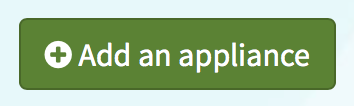
\includegraphics[width=0.25\columnwidth]{images/chameleon/Add-an-appliance.png}

You will be prompted to enter a name, description, and documentation.
Instead of providing appliance IDs, copy your template to the dedicated
field. Finally, share your contact information and assign a version
string to your appliance. Once submitted, your appliance will be
reviewed. We will get in touch if a change is needed, but if it's all
good we will publish it right away!

\section{Advanced topics}\label{advanced-topics}

\subsection{All-to-all information
exchange}\label{all-to-all-information-exchange}

The previous examples have all used user-data scripts to provide
instances with contextualization information. While it is easy to use,
this contextualization method has a major drawback: because it is given
to the instance as part of its launch request, it cannot use any context
information that is not yet known at this time.

In practice, this means that in a client-server deployment, only one of
these pattern will be possible:

\begin{itemize}
\item
  The server has to be deployed first, and once it is deployed, the
  clients can be launched and contextualized with information from the
  server. The server won't know about the clients unless there is a
  mechanism (not managed by Heat) for the client to contact the server.
\item
  The clients have to be deployed first, and once they are deployed, the
  server can be launched and contextualized with information from the
  clients. The clients won't know about the server unless there is a
  mechanism (not managed by Heat) for the server to contact the clients.
\end{itemize}

This limitation was already apparent in our NFS share~appliance: this is
why the server instance exports the file system to all bare-metal
instances on Chameleon, because it doesn't know which specific IP
addresses are allocated to the clients.

This limitation is even more important if the deployment is not
hierarchical, i.e. all instances need to know about all others. For
example, a cluster with IP and hostnames populated in /etc/hosts
required each instance to be known by every other instance.

This section presents a more advanced form of contextualization that can
perform this kind of information exchange. This is implemented by Heat
agents running inside instances and communicating with the Heat service
to send and receive information. This means you will need to use an
image bundling these agents. Currently, our CC-CentOS7 appliance and its
CUDA version are the only ones supporting this mode of
contextualization. If you build your own images using the
\href{https://github.com/ChameleonCloud/CC-CentOS7}{CC-CentOS7 appliance
builder}, you will automatically have these agents installed.

This contextualization is performed with several Heat resources:

\begin{itemize}
\item
  \texttt{OS::Heat::SoftwareConfig}.~This resource describes code to run
  on an instance. It can be configured with inputs and provide outputs.
\item
  \texttt{OS::Heat::SoftwareDeployment}. This resource applies a
  SoftwareConfig to a specific instance.
\item
  \texttt{OS::Heat::SoftwareDeploymentGroup}. This resource applies a
  SoftwareConfig to a specific group of instances.
\end{itemize}

The template below illustrates how it works. It launches a group of
instances that will automatically populates their /etc/hosts file with
IP and hostnames from other instances in the deployment.

\begin{footnotesize}
\begin{verbatim}
heat_template_version: 2015-10-15

description: >
  This template demonstrates how to exchange hostnames and IP addresses to populate /etc/hosts.

parameters:
  flavor:
    type: string
    default: baremetal
    constraints:
    - custom_constraint: nova.flavor
  image:
    type: string
    default: CC-CentOS7
    constraints:
    - custom_constraint: glance.image
  key_name:
    type: string
    default: default
    constraints:
    - custom_constraint: nova.keypair
  instance_count:
    type: number
    default: 2
  reservation_id:
    type: string
    description: ID of the Blazar reservation to use for launching instances.
    constraints:
    - custom_constraint: blazar.reservation

resources:
  export_hosts:
    type: OS::Heat::SoftwareConfig
    properties:
      outputs:
        - name: hosts
      group: script
      config: |
        #!/bin/sh
        (echo -n $(facter ipaddress); echo -n ' '; echo $(facter hostname)) > ${heat_outputs_path}.hosts

  export_hosts_sdg:
    type: OS::Heat::SoftwareDeploymentGroup
    properties:
      config: { get_resource: export_hosts }
      servers: { get_attr: [server_group, refs_map] }
      signal_transport: HEAT_SIGNAL

  populate_hosts:
    type: OS::Heat::SoftwareConfig
    properties:
      inputs:
        - name: hosts
      group: script
      config: |
        #!/usr/bin/env python
        import ast
        import os
        import string
        import subprocess
        hosts = os.getenv('hosts')
        if hosts is not None:
            hosts = ast.literal_eval(string.replace(hosts, '\n', '\\n'))
        with open('/etc/hosts', 'a') as hosts_file:
          for ip_host in hosts.values():
              hosts_file.write(ip_host.rstrip() + '\n')

  populate_hosts_sdg:
    type: OS::Heat::SoftwareDeploymentGroup
    depends_on: export_hosts_sdg
    properties:
      config: { get_resource: populate_hosts }
      servers: { get_attr: [server_group, refs_map] }
      signal_transport: HEAT_SIGNAL
      input_values:
        hosts: { get_attr: [ export_hosts_sdg, hosts ] }

  server_group:
    type: OS::Heat::ResourceGroup
    properties:
      count: { get_param: instance_count }
      resource_def:
        type: OS::Nova::Server
        properties:
          flavor: { get_param: flavor }
          image: { get_param: image }
          key_name: { get_param: key_name }
          networks:
             - network: sharednet1
          scheduler_hints: { reservation: { get_param: reservation_id } }
          user_data_format: SOFTWARE_CONFIG
          software_config_transport: POLL_SERVER_HEAT

outputs:
  deployment_results:
    value: { get_attr: [export_hosts_sdg, hosts] }
\end{verbatim}
\end{footnotesize}

There are two SoftwareConfig resources.

The first SoftwareConfig, export\_hosts, uses the facter tool to extract
IP address and hostname into a single line (in the format expected for
/etc/hosts) and writes it to a special path
(\$\{heat\_outputs\_path\}.hosts). This prompts Heat to assign the
content of this file to the output with the name hosts.

The second SoftwareConfig, populate\_hosts, takes as input a variable
named hosts, and applies a script that reads the variable from the
environment, parses it with ast.literal\_eval (as it is formatted as a
Python dict), and writes each value of the dictionary to /etc/hosts.

The SoftwareDeploymentGroup resources export\_hosts\_sdg and
populate\_hosts\_sdg apply each SoftwareConfig to the instance
ResourceGroup with the correct configuration.

Finally, the instance ResourceGroup is configured so that each instance
uses the following contextualization method instead of a user-data
script:

\begin{footnotesize}
\begin{verbatim}
          user_data_format: SOFTWARE_CONFIG
          software_config_transport: POLL_SERVER_HEAT
\end{verbatim}
\end{footnotesize}

You can follow the same template pattern to configure your own
deployment requiring all-to-all information exchange.



\FILENAME

\section{Bare Metal}\label{C:cc-baremetal}

In this page you will find documentation guiding you through the
bare-metal deployment features available in~Chameleon. Chameleon gives
users administrative access to bare-metal compute resources to
run~{cloud computing~}experiments with a high degree of customization
and repeatability. Typically, an experiment will go through several
phases, as illustrated in the figure below:


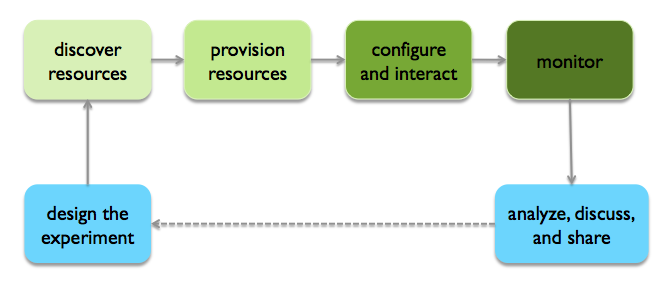
\includegraphics[width=\columnwidth]{images/chameleon/baremetal.png}


The bare-metal user guide comes in two editions. The first is how to use
Chameleon resources~via the web interface, the recommended choice for
new users to quickly learn how to use our testbed:

\textbf{\href{https://www.chameleoncloud.org/discover-resources}{Get
started with Chamelon using the web interface}}

\begin{enumerate}
\item
  \href{https://www.chameleoncloud.org/discover-resources/}{Discover
  Resources}
\item
  \href{https://www.chameleoncloud.org/provision-resources/}{Provision
  Resources}~
\item
  \href{https://www.chameleoncloud.org/configure-and-interact/}{Configure
  and Interact}
\item
  \href{https://www.chameleoncloud.org/monitor-and-collect/}{Monitor and
  Collect Results}
\end{enumerate}

The second targets~advanced users who are already familiar with
Chameleon~and would like to learn how to use Chameleon from the~command
line or with scripts.

\href{https://www.chameleoncloud.org/discover-resources-command-lines}{Get
started with Chameleon using the command line~(advanced)}

\begin{enumerate}
\item
  \href{https://www.chameleoncloud.org/discover-resources-command-lines/}{Discover
  Resources}
\item
  \href{https://www.chameleoncloud.org/advanced-provision-resources/}{Provision
  Resources}
\item
  \href{https://www.chameleoncloud.org/advanced-configure-and-interact/}{Configure
  and Interact}
\item
  \href{https://www.chameleoncloud.org/monitor-and-collect/}{Monitor and
  Collect Results}
\end{enumerate}

You do not need to strictly follow the documentation~sequentially.
However, note that some steps assume that~previous ones have been
successfully performed.

You can also consult~documentation~describing how to use advanced
features of Chameleon not covered by the guides above:

\begin{itemize}
\item
  the
  \href{https://www.chameleoncloud.org/docs/bare-metal-user-guide/chameleon-object-store/}{Chameleon
  Object Store},
\item
  \href{https://www.chameleoncloud.org/docs/bare-metal-user-guide/network-isolation-bare-metal/}{network
  isolation for bare metal}.
\end{itemize}





\section{Frequently Asked Questions}\label{frequently-asked-questions}

\FILENAME

\subsection{Appliances}\label{appliances}

\subsubsection{What is an appliance?}\label{what-is-an-appliance}

An appliance is an application packaged together with the environment
that this application requires. For example, an appliance can consists
of the operating system, libraries and tools used by the application,
configuration features such as environment variable settings, and the
installation of the application itself. Examples of appliances might
include a KVM virtual machine image, a Docker image, or a bare metal
image. Chameleon appliance refers to bare metal images that can be
deployed on the Chameleon testbed. Since an appliance captures the
experimental environment exactly, it is a key element of
reproducibility; publishing an appliance used to obtain experimental
results will go a long way to allowing others to reproduce and build on
your research easily.

To deploy distributed applications on several Chameleon instances,
complex appliances combine an image and a template describing how the
cluster should be configured and contextualized. You can read more about
them in the
\href{https://www.chameleoncloud.org/docs/complex-appliances/}{Complex
Appliances documentation}.

\subsubsection{What is the Appliance Catalog?}\label{what-is-the-chameleon-appliance-catalog}

\href{https://www.chameleoncloud.org/appliances/}{The Chameleon
Appliance Catalog} is a repository that allows users to discover,
publish, and share appliances. The appliance catalog contains useful
images of both bare metal and virtual machine appliances supported by
the Chameleon team as well appliances contributed by users.

\subsubsection{How do I publish an appliance in the Appliance Catalog?}\label{how-do-i-publish-an-appliance-in-the-chameleon-appliance-catalog}

The new Appliance Catalog allows you to easily publish and share your
own appliances so that others can discover them and use them either to
reproduce the research of others or as a basis for their own research.
 Before creating your own appliance it is advisable to review other
appliances on
the \href{https://www.chameleoncloud.org/appliances/}{Chameleon
Appliance Catalog} in order to get an idea of the categories you will
want to contribute and what others have done. 

Once you are ready to proceed, an appliance can be contributed to
Chameleon in the following steps:

\begin{enumerate}

\item
  Create the appliance itself. You may want to test it as well as give
  some thought to what support you are willing to provide for the
  appliance (e.g., if your group developed and supports a software
  package, the appliance may be just a new way of packaging the software
  and making it available, in which case your standard support channels
  may be appropriate for the appliance as well).
\item
  Upload the appliance to the Chameleon Image Repository (Glance) and
  make the image public. In order to enter the appliance into the
  Catalog you will be asked to provide the Glance ID for the image.
  These IDs are per-cloud, so that there are three options right now:
  bare metal/CHI at University of Chicago, bare metal/CHI at TACC, and
  OpenStack/KVM at TACC. You will need to provide at least one
  appliance, but may want to provide all three.
\item
  Go to
  the \href{https://www.chameleoncloud.org/appliances/create/}{Appliance
  Catalog Create Appliance web form}, fill out, and submit the form. Be
  prepared to provide the following information: a descriptive name
  (this sometimes requires some thought!), author and support contact,
  version, and an informative description. The description is a very
  important part of the appliance record; others will use it to evaluate
  if the appliance contains tools they need for their research so it
  makes sense to prepare it carefully. To make your description
  effective you may want to think of the following questions: what does
  the appliance contain? what are the specific packages and their
  versions? what is it useful for? where can it be deployed and/or what
  restrictions/limitations does it have? how should users connect to it
  / what accounts are enabled?
\end{enumerate}

If you are adding a complex appliance, skip the image ID fields and
enter your template instead in the dedicated text box.

As always, if you encounter any problems or want to share with us
additional improvements we should do to the process, please don't
hesitate to \href{https://www.chameleoncloud.org/help/}{submit a
ticket}. 

\subsubsection{How can I manage an appliance on Appliance
Catalog?}\label{how-can-i-manage-an-appliance-on-chameleon-appliance-catalog}

If you are the owner of the appliance, you can edit the appliance
data, such as the description or the support information. Browse to the
appliance that you want to edit and view its Details page. At the top
right of the page is an Edit button. You will be presented with the same
web form as when creating the appliance, pre-filled with the appliances
current information. Make changes as necessary and click Save at the
bottom of the page.

And finally, you can delete appliances you had made available. {Browse
to the appliance that you want to delete and click Edit on the
Appliance Details page. At the bottom of the page is a Delete button.
You will be asked to confirm once more that you do want to delete this
appliance}. After confirming, the appliance will be removed and no
longer listed on the Appliance Catalog.

\subsubsection{Why are there different image IDs  for the same
appliance?}\label{why-are-there-different-image-ids-for-kvmtacc-chitacc-and-chiuc-for-the-same-appliance}

The three clouds forming the Chameleon testbed are fully separated, each
having its own Glance image repository. The same appliance
image uploaded to the three clouds will produce three different image
IDs.

In addition, it is sometimes needed to customize an appliance image for
each site, resulting in slightly different image files.

\subsubsection{Can I use another operating system on bare-metal?}\label{can-i-useubuntudebian-oranother-operating-system-rather-than-centos-on-bare-metal}

The recommended appliance for Chameleon is CentOS 7 (supported by
Chameleon staff), or appliances built on top of it.\\
These appliances provide Chameleon-specific customizations, such as
login using the cc account, the cc-checks utility to verify hardware
against our resource registry, gathering of metrics, etc.

Since 2016, we also provide and support Ubuntu 14.04 and
16.04 appliances with the same functionality.

\subsection{Bare Metal Troubleshooting}\label{bare-metal-troubleshooting}

\subsubsection{Why are my Bare Metal instances failing to
launch?}\label{why-are-my-bare-metal-instances-failing-to-launch}

The Chameleon Bare Metal clouds require users to reserve resources
before allowing them to launch instances. Please follow the
\href{https://www.chameleoncloud.org/docs/bare-metal/}{documentation}
and make sure that:

\begin{enumerate}
\item
  You have created a lease and it has started (the associated
  reservation is shown as \textbf{Active})
\item
  You have selected your reservation in the \textbf{Launch Instance}
  panel
\end{enumerate}

If you still cannot start instances, please
\href{https://www.chameleoncloud.org/user/help/}{open a ticket with our
help desk}.

\subsection{OpenStack KVM Troubleshooting}\label{openstack-kvm-troubleshooting}

\subsubsection{Why are my OpenStack KVM instances failing to
launch?}\label{why-are-my-openstack-kvm-instances-failing-to-launch}

If you get an error stating that \textbf{No valid host was found}, it
might be caused by a lack of resources in the cloud. The Chameleon staff
continuously monitors the utilization of the testbed, but there might be
times when no more resources are available. If the error persists,
please \href{https://www.chameleoncloud.org/user/help/}{open a ticket
with our help desk}.

\subsubsection{Why can't I ping or SSH to my
instance?}\label{why-cant-i-ping-or-ssh-to-my-instance}

While the possibility that the system is being taking over by nanites
should not be discounted too easily, it is always prudent to first
check for the following issues:

\begin{itemize}
\item
  Do you have a floating IP associated with your instance? By default,
  instances do not have publicly-accessible IP addresses assigned. See
  the \textbf{Managing Virtual Machine Instances} section in the
  \href{https://www.chameleoncloud.org/docs/user-guides/openstack-kvm-user-guide/}{User
  Guide}.
\item
  Does your security group allow incoming ICMP (e.g. ping) traffic? By
  default, firewall rules do not allow ping to your instances. If you
  wish to enable it, see the \textbf{Firewall (Access Security)} section
  in the
  \href{https://www.chameleoncloud.org/docs/user-guides/openstack-kvm-user-guide/}{User
  Guide}.
\item
  Does your security group allow incoming SSH (TCP port 22) traffic? By
  default, firewall rules do not allow SSH to your instances. If you
  wish to enable it, see the \textbf{Firewall (Access Security)} section
  in the
  \href{https://www.chameleoncloud.org/docs/user-guides/openstack-kvm-user-guide/}{User
  Guide}.
\end{itemize}

 If none of these solve your problem,
please \href{https://www.chameleoncloud.org/user/help/}{open a ticket
with our help desk}, and send us the results of the above (and any
evidence of nanites you find as well).





\begin{comment}



%\section{How to use Git in this class}\label{how-to-use-git-in-this-class}

Let us use the first homework `TechList 1' as an example to illstrate
why and how we choose Git as a essential tool in this class.

In the `Technologies' section on the class website, we will
collaboratively edit the web page contents. Each student shall add their
paragraphs about certain tech topics. This leads to a question: multiple
authors are working on a same document, whose version should be used as
the final version? After all, there can only be one version published
online.

Git can largely (not completely) help use sort it out. And here is our
Git workflow:

\subsection{Step 1}\label{step-1}

In the class official repo, we start from an empty TechList file. Here
is the file we start from in our class repo:
\url{https://github.com/cloudmesh/classes/blob/master/docs/source/i524/technologies.rst}

\subsection{Step 2}\label{step-2}

Each student is going to create a repository exactly the same as the
official repo. This step is called to `fork' the repo. You do so by
click the `fork' button on the top right corner of the page. Once done,
you have your own copy of the class repo.

\subsection{Step 3}\label{step-3}

You create this repo in your Github account. This means you still store
everything online remotely.

\subsection{Step 4}\label{step-4}

To conveniently edit the files, you need a copy on your laptop. This is
to `clone' your personal repo to your local disk. Look at your Github
repo and find a green button saying `clone or download'. Click this
button and you will have a pulldown menu where you should copy the URL.
In your terminal/commandline, run `git clone \textless{}the URL you just
copied\textgreater{}'. This step copies the project to your own disk for
editing.

\subsection{Step 5}\label{step-5}

Your local copy is a `live' version, since you are going to keep editing
it. Put your contents in the `technologies.rst' file in the
corresponding sections.

\subsection{Step 6}\label{step-6}

At any point during your editing, if you want to secure the changes you
made to the file, you can always `commit'. Refer to the `git commit'
instruction. Obviously, when you finish all the typing, a `commit'
operation must be performed. Consider a `commit' operation a fancy
`save' operation you may always do during file editing. A major
advantage is, `commit' will keep a history of all the versions you
committed. All the committed texts will not be lost. This reduces a lot
of risks during long term, large scale development.

\subsection{Step 7}\label{step-7}

When you complete your work, it is the time to submit your homework back
to the graders. Do this in two steps. First, you have to `push' your
local disk copy to the repo you created under your acount in step 4).
Follow closely after this link
\url{https://github.com/cloudmesh/classes\#submitting-changes} to get
your local disk and your personal remote a.k.a. the `origin'
synchronized. Second step is done via your browser. At the very top of
your repo web page, switch to the `Pull requests' tab, and submit a pull
request to the class repo. This way, the instructor will get notified
and merge your repo into the class official repo. After this merge being
performed, all your contributions will be included into the public site.


\part{Python}

%----------------------------------------------------------------------------------------
%	PART
%----------------------------------------------------------------------------------------
\chapterimage{python-logo-generic.pdf} % Chapter heading image


\part{Python}
\label{P:python}


%----------------------------------------------------------------------------------------
%	CHAPTER 1
%----------------------------------------------------------------------------------------

\chapter{Introduction}
\FILENAME

\FILENAME

\section{Introduction to Python}\label{introduction-to-python}
\index{Python}

Portions of this lesson have been adapted from the
\href{https://docs.python.org/2/tutorial/}{official Python Tutorial}
copyright \href{http://www.python.org/}{Python Software Foundation}.

Python is an easy to learn programming language. It has efficient
high-level data structures and a simple but effective approach to
object-oriented programming. Python's simple syntax and dynamic typing,
together with its interpreted nature, make it an ideal language for
scripting and rapid application development in many areas on most
platforms. The Python interpreter and the extensive standard library are
freely available in source or binary form for all major platforms from
the Python Web site, \url{https://www.python.org/}, and may be freely
distributed. The same site also contains distributions of and pointers
to many free third party Python modules, programs and tools, and
additional documentation. The Python interpreter can be extended with
new functions and data types implemented in C or C++ (or other languages
callable from C). Python is also suitable as an extension language for
customizable applications.

Python is an interpreted, dynamic, high-level programming language
suitable for a wide range of applications.

The philosophy of python is summarized in
\href{https://www.python.org/dev/peps/pep-0020/}{The Zen of Python} as
follows:

\begin{itemize}

\item
  Explicit is better than implicit
\item
  Simple is better than complex
\item
  Complex is better than complicated
\item
  Readability counts
\end{itemize}

The main features of Python are:

\begin{itemize}

\item
  Use of indentation whitespace to indicate blocks
\item
  Object orient paradigm
\item
  Dynamic typing
\item
  Interpreted runtime
\item
  Garbage collected memory management
\item
  a large standard library
\item
  a large repository of third-party libraries
\end{itemize}

Python is used by many companies (such as Google, Yahoo!, CERN, NASA)
and is applied for web development, scientific computing, embedded
applications, artificial intelligence, software development, and
information security, to name a few.

The material collected here introduces the reader to the basic concepts and
features of the Python language and system. After you have worked
tthrough the material you will be able to:

\begin{itemize}

\item
  use Python
\item
  use the interactive Python interface
\item
  understand the basic syntax of Python
\item
  write and run Python programs stored in a file
\item
  have an overview of the standard library
\item
  install Python libraries using pyenv or if it is not available
  virtualenv
\end{itemize}

This tutorial does not attempt to be comprehensive and cover every
single feature, or even every commonly used feature. Instead, it
introduces many of Python's most noteworthy features, and will give you
a good idea of the language's flavor and style. After reading it, you
will be able to read and write Python modules and programs, and you will
be ready to learn more about the various Python library modules.

In order to conduct this lesson you need

\begin{itemize}

\item
  A computer with Python 2.7.13 or 3.6.2
\item
  Familiarity with command line usage
\item
  A text editor such as
  \href{https://www.jetbrains.com/pycharm/}{PyCharm}, emacs, vi or
  others. You should identity which works best for you and set it up.
\end{itemize}

\section{Refernces}
\index{Python!Refernces}

Some important additional information can be found on the following
Web pages.

\begin{itemize}
\item \href{https://www.python.org/}{Python}
\item \href{https://pip.pypa.io/en/stable/}{Pip}
\item \href{https://virtualenv.pypa.io/en/stable/}{Virtualenv}
\item \href{http://www.numpy.org/}{NumPy}
\item \href{https://scipy.org/}{SciPy}
\item \href{http://matplotlib.org/}{Matplotlib}
\item \href{http://pandas.pydata.org/}{Pandas}
\item \href{https://github.com/pyenv/pyenv}{pyenv}
\item \href{https://github.com/pyenv/pyenv}{PyCharm}
\end{itemize}

Python module of the week is a Web site that provides a number of short
examples on how to use some elementary python modules. Not all modules
are equally useful and you should decide if there are better
alternatives. However for beginners this site provides a number of good
examples

\begin{itemize}

\item
  Python 2: \url{https://pymotw.com/2/}
\item
  Python 3: \url{https://pymotw.com/3/}
\end{itemize}


\chapter{Install}

\FILENAME\

\section{Python Installation}\label{python-installation}
\index{Python!Install}

Python is easy to install and very good instructions for most platforms
can be found on the python.org Web page. We will be using Python 2.7.13
and/or Python 3 in our activities.

To manage python modules, it is useful to have
\href{https://pypi.python.org/pypi/pip}{pip} package installation tool
on your system.

In the tutorial, we assume that you have a computer with python
installed. However, we also recommend that for the class you use
Python's virtualenv (see below) to isolate your development Python from
the system installed Python.

\subsection{Managing custom Python
installs}\label{managing-custom-python-installs}

Often you have your own computer and you do not like to change its
environment to keep it in pristine condition. Python comes with many
libraries that could for example conflict with libraries that you have
installed. To avoid this it is bets to work in an isolated python we can
use tools such as virtualenv, pyenv or pyvenv for 3.6.4\footnote{check
  for the newest version}. Which you use
depends on you, but we highly recommend pyenv if you can.

\subsubsection{Managing Multiple Python Versions with
Pyenv}
\label{S:managing-multiple-python-versions-with-pyenv}
\index{pyenv}

Python has several versions that are used by the community. This
includes Python 2 and Python 3, but alls different management of the
python libraries. As each OS may have their own version of python
installed. It is not recommended that you modify that version. Instead
you may want to create a localized python installation that you as a
user can modify. To do that we recommend \emph{pyenv}. Pyenv allows
users to switch between multiple versions of Python
(\url{https://github.com/yyuu/pyenv}). To summarize:

\begin{itemize}

\item
  users to change the global Python version on a per-user basis;
\item
  users to enable support for per-project Python versions;
\item
  easy version changes without complex environment variable management;
\item
  to search installed commands across different python versions;
\item
  integrate with tox (\url{https://tox.readthedocs.io/}).
\end{itemize}

\paragraph{Instalation without pyenv}\label{instalation-without-pyenv}

If you need to have more than one python version installed and do not
want or can use pyenv, we recommend you download and install python
2.7.13 and 3.6.4\footnote{check
  for the newest version} from python.org
(\url{https://www.python.org/downloads/})

\paragraph{Disabeling wrong python installs on
OSX}\label{disabeling-wrong-python-installs-on-osx}

While working with students we have seen at times that they take other
classes either at universities or online that teach them how to program
in python. Unfortunately, although they seem to do that they often
ignore to teach you how to properly install python. I just recently had
a students that had installed python 7 times on his OSX machine, while
another student had 3 different installations, all of which confliced
with each other as they were not set up properly.

We recommend that you inspect if you have a files such as
\verb|~/.bashrc| or \verb|~/.bashrc_profile| in your
home directory and identify if it activates various versions of python
on your computer. If so you could try to deactivate them while
out-commenting the various versions with the \# character at the
beginning of the line, start a new terminal and see if the terminal
shell still works. Than you can follow our instructions here while using
an install on pyenv.

\paragraph{Install pyenv on OSX from
git}\label{install-pyenv-on-osx-from-git}

This is our recommended way to install pyenv on OSX:

\begin{verbatim}
$ git clone https://github.com/pyenv/pyenv.git ~/.pyenv
$ git clone https://github.com/pyenv/pyenv-virtualenv.git ~/.pyenv/plugins/pyenv-virtualenv
$ git clone https://github.com/yyuu/pyenv-virtualenvwrapper.git ~/.pyenv/plugins/pyenv-virtualenvwrapper
$ echo 'export PYENV_ROOT="$HOME/.pyenv"' >> ~/.bash_profile
$ echo 'export PATH="$PYENV_ROOT/bin:$PATH"' >> ~/.bash_profile
\end{verbatim}

\paragraph{Installation of Homebrew}\label{instalation-of-homebrew}

Before installing anything on your computer make sure you have enough
space. Use in the terminal the command:

\begin{verbatim}
$ df -h
\end{verbatim}

which gives your an overview of your file system. If you do not have
enough space, please make sure you free up unused files from your drive.

In many occasions it is beneficial to use readline as it provides nice
editing features for the terminal and xz for completion. First, make
sure you have xcode installed:

\begin{verbatim}
$ xcode-select --install
\end{verbatim}

Next install homebrew, pyenv, pyenv-virtualenv and pyenv-virtualwrapper.
Additionally install readline and some compression tools:

\begin{verbatim}
/usr/bin/ruby -e "$(curl -fsSL https://raw.githubusercontent.com/Homebrew/install/master/install)"
brew update
brew install readline xz
\end{verbatim}

\paragraph{Install pyenv on OSX with
Homebrew}\label{install-pyenv-on-osx-with-homebrew}

We describe here a mechanism of installing pyenv with homebrew. Other
mechanisms can be found on the pyenv documentation page
(\url{https://github.com/yyuu/pyenv-installer}). You must have homebrew
installed as discussed in the previous section.

To install pyenv with homebrew execute in the terminal:

\begin{verbatim}
brew install pyenv pyenv-virtualenv pyenv-virtualenvwrapper
\end{verbatim}

\paragraph{Install pyenv on Ubuntu}\label{install-pyenv-on-ubuntu}

The following steps will install pyenv in a new ubuntu 16.04
distribution.

Start up a terminal and execute in the terminal the following commands.
We recommend that you do it one command at a time so you can observe if
the command succeeds:

\begin{verbatim}
$ sudo apt-get update
$ sudo apt-get install git python-pip make build-essential libssl-dev
$ sudo apt-get install zlib1g-dev libbz2-dev libreadline-dev libsqlite3-dev
$ sudo pip install virtualenvwrapper

$ git clone https://github.com/yyuu/pyenv.git ~/.pyenv
$ git clone https://github.com/pyenv/pyenv-virtualenv.git ~/.pyenv/plugins/pyenv-virtualenv   
$ git clone https://github.com/yyuu/pyenv-virtualenvwrapper.git ~/.pyenv/plugins/pyenv-virtualenvwrapper

$ echo 'export PYENV_ROOT="$HOME/.pyenv"' >> ~/.bashrc
$ echo 'export PATH="$PYENV_ROOT/bin:$PATH"' >> ~/.bashrc
\end{verbatim}

Now that you have installed pyenv it is not yet activated in your
current terminal. The easiest thing to do is to start a new terminal and
typ in:

\begin{verbatim}
which pyenv
\end{verbatim}

If you see a response pyenv is installed and you can proceed with the
next steps.

Please remember whenever you modify \verb|.bashrc| or
\verb|.bash_profile| you need to start a new terminal.

\paragraph{Install Different Python
Versions}\label{install-different-python-versions}

Pyenv provides a large list of different python versions. To see the
entire list please use the command:

\begin{verbatim}
$ pyenv install -l
\end{verbatim}

However, for us we only need to worry about python 2.7.13 and python
3.6.4\footnote{check
  for the newest version}. You can now
install different versions of python into your local environment with
the following commands:

\begin{verbatim}
$ pyenv install 2.7.13
$ pyenv install 3.6.4
\end{verbatim}

You can set the global python default version with:

\begin{verbatim}
$ pyenv global 2.7.13
\end{verbatim}

Type the following to determine which version you activated:

\begin{verbatim}
$ pyenv version
\end{verbatim}

Type the following to determine which versions you have available:

\begin{verbatim}
$ pyenv versions
\end{verbatim}

Associate a specific environment name with a certain python version, use
the following commands:

\begin{verbatim}
$ pyenv virtualenv 2.7.13 ENV2
$ pyenv virtualenv 3.6.4 ENV3
\end{verbatim}

In the example above, ENV2 would represent python 2.7.13 while ENV3
would represent python 3.6.4. Often it is easier to type the alias
rather than the explicit version.

\paragraph{Set up the Shell}\label{s:set-up-the-shell}

To make all work smoothly from your terminal, you can include the
following in your \verb|.bashrc| files:

\begin{verbatim}
export PYENV_VIRTUALENV_DISABLE_PROMPT=1
eval "$(pyenv init -)"
eval "$(pyenv virtualenv-init -)"

__pyenv_version_ps1() {
  local ret=$?;
  output=$(pyenv version-name)
  if [[ ! -z $output ]]; then
    echo -n "($output)"
  fi
  return $ret;
}

PS1="\$(__pyenv_version_ps1) ${PS1}"
\end{verbatim}

We recommend that you do this towards the end of your file.

\paragraph{Switching Environments}\label{switching-environments}

After setting up the different environments, switching between them is
now easy. Simply use the following commands:

\begin{verbatim}
(2.7.13) $ pyenv activate ENV2
(ENV2) $ pyenv activate ENV3
(ENV3) $ pyenv activate ENV2
(ENV2) $ pyenv deactivate ENV2
(2.7.13) $ 
\end{verbatim}

To make it even easier, you can add the following lines to your
\verb|.bash_profile| file:

\begin{verbatim}
alias ENV2="pyenv activate ENV2"
alias ENV3="pyenv activate ENV3"
\end{verbatim}

If you start a new terminal, you can switch between the different
versions of python simply by typing:

\begin{verbatim}
$ ENV2
$ ENV3
\end{verbatim}

\subsection{Updating Python Version List}

Pyenv maintains locally a list of available python versions. To see
the list use the command

\begin{lstlisting}
pyenv install -l
\end{lstlisting}

To obtain the newest list please use the command

\begin{lstlisting}
cd ~/.pyenv/plugins/python-build/../.. && git pull
\end{lstlisting}

Now when you call 

\begin{lstlisting}
pyenv install -l
\end{lstlisting}

You will see the updated list.

\subsection{Updating to a new version of Python with pyenv}

Naturally pyyhon itself evolves and new versions will become available
via pyenv. To facilitate such a new version you need to first install
it. into pyenv. Let us assume you had an old version of python
installed onto the ENV3 environment. Than you need to execute the
following steps:

\begin{lstlisting}
pyenv deactivate
pyenv uninstall ENV3
pyenv install 3.6.4
pyenv virtualenv 3.6.4 ENV3
\begin{lstlisting}

In case you get an error, you may have to update xcode as follows and
try again:

\begin{lstlisting}
xcode-select --install
\end{lstlisting}


After you installed it you can activate it by typing
\verb|ENV3|. Naturally this requires that you added it to your bash
environment as discussed in Section~\ref{s:set-up-the-shell}.

\subsection{Installation without pyenv}

If you need to have more than one python version installed and do not
want or can use pyenv, we recommend you download and install python
2.7.13 and 3.6.4 from python.org
(\url{https://www.python.org/downloads/})

\subsubsection{Make sure pip is up to date}

As you will want to install other packages, make sure pip is up to date:

\begin{verbatim}
pip install pip -U
\end{verbatim}

pyenv virtualenv anaconda3-4.3.1 ANA3 pyenv activate ANA3

\subsection{Anaconda and Miniconda}\label{anaconda-and-miniconda}

\begin{description}
\item[We do not recommend that you use anaconda or miniconda as it may]
interfere with your default python interpreters and setup.
\end{description}

Please note that beginners to pyton should always use anaconda or
miniconda only afterthey have installed pyenv and use it. For this class
neither anaconda nor miniconda is required. In fact we do not recommend
it. We keep this section as we know that other classes at IU may use
anaconda. We are not aware if these classes teach you the right way to
install it, with \emph{pyenv}.

\subsubsection{Miniconda}\label{miniconda}

\begin{description}
\item[This section about miniconda is experimental and has not]
been tested. We are looking for contributors that help completing it. If
you use anaconda or miniconda we recommend to manage it via pyenv.
\end{description}

To install mini conda you can use the following commands:

\begin{verbatim}
$ mkdir ana
$ cd ana
$ pyenv install miniconda3-latest
$ pyenv local miniconda3-latest
$ pyenv activate miniconda3-latest
$ conda create -n ana anaconda
\end{verbatim}

To activate use:

\begin{verbatim}
$ source activate ana
\end{verbatim}

To deactivate use:

\begin{verbatim}
$ source deactivate
\end{verbatim}

To install cloudmesh cmd5 please use:

\begin{verbatim}
$ pip install cloudmesh.cmd5
$ pip install cloudmesh.sys
\end{verbatim}

\subsubsection{Anaconda}\label{anaconda}

\begin{description}
\item[This section about anaconda is experimental and has not]
been tested. We are looking for contributors that help completing it.
\end{description}

You can add anaconda to your pyenv with the following commands:

\begin{verbatim}
pyenv install anaconda3-4.3.1
\end{verbatim}

To switch more easily we recommend that you use the following in your
\verb|.bash_profile| file:

\begin{verbatim}
alias ANA="pyenv activate anaconda3-4.3.1"
\end{verbatim}

Once you have done this you can easily switch to anaconda with the
command:

\begin{verbatim}
$ ANA
\end{verbatim}

Terminology in annaconda could lead to confusion. Thus we like to point
out that the version number of anaconda is unrelated to the python
version. Furthermore, anaconda uses the term root not for the root user,
but for the originating directory in which the anaconda program is
installed.

In case you like to build your own conda packages at a later time we
recommend that you install the conda-build package:

\begin{verbatim}
$ conda install conda-build
\end{verbatim}

When executing:

\begin{verbatim}
pyenv versions
\end{verbatim}

you will see after the install completed the anaconda versions
installed:

\begin{verbatim}
pyenv versions
system
2.7.13
2.7.13/envs/ENV2
3.6.4
3.6.4/envs/ENV3
ENV2 
ENV3
* anaconda3-4.3.1 (set by PYENV_VERSION environment variable)
\end{verbatim}

Let us now create virtualenv for anaconda:

\begin{verbatim}
$ pyenv virtualenv anaconda3-4.3.1 ANA
\end{verbatim}

To activate it you can now use:

\begin{verbatim}
$ pyenv ANA
\end{verbatim}

However, anaconda may modify your \verb|.bashrc| or \verb|.bash_profile| files and
may result in incompatibilities with other python versions. For this
reason we recommend not to use it. If you find ways to get it to work
reliably with other versions, please let us know and we update this
tutorial.

To install cloudmesh cmd5 please use:

\begin{verbatim}
$ pip install cloudmesh.cmd5
$ pip install cloudmesh.sys
\end{verbatim}

\paragraph{Exercise}

\begin{exercise}
Write installation instructions for an operating system of your choice
and add to this documentation.
\end{exercise}

\begin{exercise}
Replicate the steps above, so you can type in ENV2 and ENV3 in your
terminals to switch between python 2 and 3.
\end{exercise}

\subsubsection{virtualenv}\label{virtualenv}
\index{virtualenv}

environment while using virtualenv,. Documentation about it can be found
at:

\begin{verbatim}
* https://virtualenv.pypa.io
\end{verbatim}

The installation is simple once you have pip installed. If it is not
installed you can say:

\begin{verbatim}
$ easy_install pip
\end{verbatim}

After that you can install the virtual env with:

\begin{verbatim}
$ pip install virtualenv
\end{verbatim}

To setup an isolated environment for example in the directory
\textasciitilde{}/ENV please use:

\begin{verbatim}
$ virtualenv ~/ENV
\end{verbatim}

To activate it you can use the command:

\begin{verbatim}
$ source ~/ENV/bin/activate
\end{verbatim}

you can put this command in your \verb|.bashrc| or \verb|.bash_profile| files so you
do not forget to activate it. Instructions for this can be
found in our lesson on Linux \verb|bashrc|.


\FILENAME

\section{Interactive Python}\label{interactive-python}
\index{Python!REPL}
\index{Python!interactive}

Python can be used interactively. You can enter the interactive mode
by entering the interactive loop by executing the command:

\begin{lstlisting}
$ python
\end{lstlisting}
% $

You will see something like the following:

\begin{lstlisting}
Python 2.7.13 (default, Nov 19 2016, 06:48:10)
[GCC 5.4.0 20160609] on linux2
Type "help", "copyright", "credits" or "license" for more information.
>>>
\end{lstlisting}

The \verb|>>>| is the prompt used by the interpreter. This is similar to
bash where commonly \verb|$| is used.

Sometimes it is convenient to show the prompt when illustrating an
example. This is to provide some context for what we are doing. If you
are following along you will not need to type in the prompt.

This interactive python process does the following:

\begin{itemize}
\item
  \emph{read} your input commands
\item
  \emph{evaluate} your command
\item
  \emph{print} the result of evaluation
\item
  \emph{loop} back to the beginning.
\end{itemize}

This is why you may see the interactive loop referred to as a
\textbf{REPL}:
\textbf{R}ead-\textbf{E}valuate-\textbf{P}rint-\textbf{L}oop.

\section{REPL (Read Eval Print Loop)}\label{repl-read-eval-print-loop}
\index{Python!REPL}

There are many different types beyond what we have seen so far, such as
\textbf{dictionaries}s, \textbf{list}s, \textbf{set}s. One handy way of
using the interactive python is to get the type of a value using
type():

\begin{lstlisting}
>>> type(42)
<type 'int'>
>>> type(hello)
<type 'str'>
>>> type(3.14)
<type 'float'>
\end{lstlisting}


You can also ask for help about something using help():

\begin{lstlisting}
>>> help(int)
>>> help(list)
>>> help(str)
\end{lstlisting}

Using help() opens up a help message within a pager. To navigate you
can use the spacebar to go down a page w to go up a page, the arrow
keys to go up/down line-by-line, or q to exit.

\section{Python 3 Features in Python 2}\label{python-3-features-in-python-2}
\index{Python!2 and 3}

In this course we want to be able to seamlessly switch between python 2
and python 3. Thus it is convenient from the start to use python 3
syntax when it is supported also in python 2. One of the most used
functions is the print statement that has in python 3 parentheses. To
enable it in python 2 you just need to import this function:

\begin{lstlisting}
>>> from __future__ import print_function, division
\end{lstlisting}

The first of these imports allows us to use the print function to output
text to the screen, instead of the print statement, which Python 2 uses.
This is simply a \href{https://www.python.org/dev/peps/pep-3105/}{design
decision} that better reflects Python's underlying philosophy.


Other functions such as the division also behave differently. Thus we use

\begin{lstlisting}
>>> from __future__ import division
\end{lstlisting}

This import makes sure that the
\href{https://www.python.org/dev/peps/pep-0238/}{division operator}
behaves in a way a newcomer to the language might find more
intuitive.  In Python 2, division / is \emph{floor division} when the
arguments are integers, meaning that the following 

\begin{lstlisting}
(5 / 2 == 2) is True
\end{lstlisting}

In Python 3, division / is a floating point division, thus 

\begin{lstlisting}
(5 / 2 == 2.5) is True
\end{lstlisting}

\chapter{Language}

\FILENAME\

\TODO{TA: some of the python examples assume REPL, but its better to use a
  print statement instead as more general, please fix}


\section{Statements and Strings}\label{statements-and-strings}
\index{Python!statements}
\index{Python!strings}


Let us explore the syntax of Python. Type into the interactive loop and
press Enter:

\begin{lstlisting}{python}
print("Hello world from Python!")
# Hello world from Python! 
\end{lstlisting}

What happened: the print function was given a \textbf{string} to
process. A string is a sequence of characters. A \textbf{character} can
be a alphabetic (A through Z, lower and upper case), numeric (any of the
digits), white space (spaces, tabs, newlines, etc), syntactic directives
(comma, colon, quotation, exclamation, etc), and so forth. A string is
just a sequence of the character and typically indicated by surrounding
the characters in double quotes.

Standard output is discussed in the \verb|../../lesson/linux/shell| lesson.

So, what happened when you pressed Enter? The interactive Python program
read the line \verb|print ("Hello world from Python!")|, split it into the print
statement and the \verb|"Hello world from Python!"| string, and then executed
the line, showing you the output.

\section{Variables}\label{variables}
\index{Python!variables}

You can store data into a \textbf{variable} to access it later. For
instance, instead of:

\begin{lstlisting}{python}
print('Hello world from Python!')
\end{lstlisting}

which is a lot to type if you need to do it multiple times, you can
store the string in a variable for convenient access:

\begin{lstlisting}{python}
hello = 'Hello world from Python!'
print(hello)
# Hello world from Python!
\end{lstlisting}

\section{Data Types}\label{data-types}
\index{Python!data types}

\subsection{Booleans}\label{booleans}
\index{Python!boolean}

A \textbf{boolean} is a value that indicates \emph{truthness} of
something. You can think of it as a toggle: either ``on'' or ``off'',
``one'' or ``zero'', ``true'' or ``false''. In fact, the only possible
values of the \textbf{boolean} (or bool) type in Python are:

\begin{itemize}

\item
  True
\item
  False
\end{itemize}

You can combine booleans with \textbf{boolean operators}:

\begin{itemize}

\item
  and
\item
  or
\end{itemize}

\begin{lstlisting}{python}
print(True and True)
# True

print(True and False)
# False

print(False and False)
# False

print(True or True)
# True

print(True or False)
# True

print(False or False)
# False
\end{lstlisting}

\subsection{Numbers}\label{numbers}
\index{Python!numbers}

The interactive interpreter can also be used as a calculator. For
instance, say we wanted to compute a multiple of 21:

\begin{lstlisting}{python}
print(21 * 2)
# 42
\end{lstlisting}

We saw here the print statement again. We passed in the result of the
operation 21 * 2. An \textbf{integer} (or \textbf{int}) in Python is a
numeric value without a fractional component (those are called
\textbf{floating point} numbers, or \textbf{float} for short).

The mathematical operators compute the related mathematical operation to
the provided numbers. Some operators are:

\begin{description}
  \item[*] --- multiplication
  \item[/] --- division
  \item[+] --- addition
  \item[-] --- subtraction
  \item[**] --- exponent
\end{description}

Exponentiation $x^y$ is written as x**y is x to the yth power.

You can combine \textbf{float}s and \textbf{int}s:

\begin{lstlisting}{python}
print(3.14 * 42 / 11 + 4 - 2)
# 13.9890909091

print(2**3)
# 8
\end{lstlisting}

Note that \textbf{operator precedence} is important. Using parenthesis
to indicate affect the order of operations gives a difference results,
as expected:

\begin{lstlisting}{python}
print(3.14 * (42 / 11) + 4 - 2)
# 11.42

print(1 + 2 * 3 - 4 / 5.0)
# 6.2

print( (1 + 2) * (3 - 4) / 5.0 )
# -0.6
\end{lstlisting}



\section{Module Management}\label{module-management}

A module allows you to logically organize your Python code. Grouping
related code into a module makes the code easier to understand and use.
A module is a Python object with arbitrarily named attributes that you
can bind and reference. A module is a file consisting of Python code. A
module can define functions, classes and variables. A module can also
include runnable code.

\subsection{Import Statement}\label{import-statement}
\index{Python!import}

When the interpreter encounters an import statement, it imports the
module if the module is present in the search path. A search path is a
list of directories that the interpreter searches before importing a
module. The from\ldots{}import Statement Python's from statement lets
you import specific attributes from a module into the current namespace.
It is preferred to use for each import its own line such as:

\begin{lstlisting}{python}
import numpy
import matplotlib
\end{lstlisting}

When the interpreter encounters an import statement, it imports the
module if the module is present in the search path. A search path is a
list of directories that the interpreter searches before importing a
module.

\subsection{The from \ldots{} import
Statement}\label{the-from-import-statement}
\index{Python!import!from}

Python's from statement lets you import specific attributes from a
module into the current namespace. The from \ldots{} import has the
following syntax:

\begin{lstlisting}{python}
from datetime import datetime   
\end{lstlisting}

\section{Date Time in Python}\label{date-time-in-python}
\index{Python!date}
\index{Python!time}

The datetime module supplies classes for manipulating dates and times in
both simple and complex ways. While date and time arithmetic is
supported, the focus of the implementation is on efficient attribute
extraction for output formatting and manipulation. For related
functionality, see also the time and calendar modules.

The import Statement You can use any Python source file as a module by
executing an import statement in some other Python source file.

\begin{lstlisting}{python}
from datetime import datetime
\end{lstlisting}

This module offers a generic date/time string parser which is able to
parse most known formats to represent a date and/or time.

\begin{lstlisting}{python}
from dateutil.parser import parse
\end{lstlisting}

pandas is an open source Python library for data analysis that needs to
be imported.

\begin{lstlisting}{python}
import pandas as pd
\end{lstlisting}

Create a string variable with the class start time

\begin{lstlisting}{python}
fall_start = '08-21-2017'
\end{lstlisting}

Convert the string to datetime format

\begin{lstlisting}{python}
datetime.strptime(fall_start, '%m-%d-%Y')
# datetime.datetime(2017, 8, 21, 0, 0)
\end{lstlisting}

Creating a list of strings as dates

\begin{lstlisting}{python}
class_dates = ['8/25/2017', '9/1/2017', '9/8/2017', '9/15/2017', '9/22/2017', '9/29/2017']
\end{lstlisting}

Convert Class\_dates strings into datetime format and save the list into
variable a

\begin{lstlisting}{python}
a = [datetime.strptime(x, '%m/%d/%Y') for x in class_dates]
\end{lstlisting}

Use parse() to attempt to auto-convert common string formats. Parser
must be a string or character stream, not list.

\begin{lstlisting}{python}
parse(fall_start)
# datetime.datetime(2017, 8, 21, 0, 0)
\end{lstlisting}

Use parse() on every element of the Class\_dates string.

\begin{lstlisting}{python}
[parse(x) for x in class_dates] 
# [datetime.datetime(2017, 8, 25, 0, 0),
#   datetime.datetime(2017, 9, 1, 0, 0),
#   datetime.datetime(2017, 9, 8, 0, 0),
#   datetime.datetime(2017, 9, 15, 0, 0),
#   datetime.datetime(2017, 9, 22, 0, 0),
#   datetime.datetime(2017, 9, 29, 0, 0)]  
\end{lstlisting}

Use parse, but designate that the day is first.

\begin{lstlisting}{python}
parse (fall_start, dayfirst=True)
# datetime.datetime(2017, 8, 21, 0, 0)
\end{lstlisting}

Create a dataframe.A DataFrame is a tabular data structure comprised of
rows and columns, akin to a spreadsheet, database table. DataFrame as a
group of Series objects that share an index (the column names).

\begin{lstlisting}{python}
import pandas as pd
data = {'class_dates': ['8/25/2017 18:47:05.069722', 
                        '9/1/2017 18:47:05.119994', 
                        '9/8/2017 18:47:05.178768', 
                        '9/15/2017 18:47:05.230071', 
                        '9/22/2017 18:47:05.230071', 
                        '9/29/2017 18:47:05.280592'], 
        'complete': [1, 0, 1, 1, 0, 1]} 
df = pd.DataFrame(data, columns = ['class_dates', 'complete'])
print(df)
#                  class_dates  complete
#  0  8/25/2017 18:47:05.069722         1
#  1   9/1/2017 18:47:05.119994         0
#  2   9/8/2017 18:47:05.178768         1
#  3  9/15/2017 18:47:05.230071         1
#  4  9/22/2017 18:47:05.230071         0
#  5  9/29/2017 18:47:05.280592         1
\end{lstlisting}

Convert \verb|df[`date`]| from string to datetime

\begin{lstlisting}{python}
import pandas as pd
pd.to_datetime(df['class_dates'])
# 0   2017-08-25 18:47:05.069722
# 1   2017-09-01 18:47:05.119994
# 2   2017-09-08 18:47:05.178768
# 3   2017-09-15 18:47:05.230071
# 4   2017-09-22 18:47:05.230071
# 5   2017-09-29 18:47:05.280592
# Name: class_dates, dtype: datetime64[ns]
\end{lstlisting}

\section{Control Statements}\label{control-statements}

\subsection{Comparison}\label{comparision}
\index{Python!if}

Computer programs do not only execute instructions. Occasionally, a
choice needs to be made. Such as a choice is based on a condition.
Python has several conditional operators:

\begin{description}
\item[>]   greater than
\item[<]   smaller than
\item[==]  equals
\item[!=]  is not
\end{description}

Conditions are always combined with variables. A program can make a
choice using the if keyword. For example:

\begin{lstlisting}{python}
x = int(input("Guess x:"))
if x == 4:
   print('You guessed correctly!')
\end{lstlisting}

In this example, \emph{You guessed correctly!} will only be printed if
the variable x equals to four (see table above). Python can also execute
multiple conditions using the elif and else keywords.

\begin{lstlisting}{python}
x = int(input("Guess x:"))
if x == 4:
    print('You guessed correctly!')
elif abs(4 - x) == 1:
    print('Wrong guess, but you are close!')
else:
    print('Wrong guess')
\end{lstlisting}

\subsection{Iteration}\label{iteration}
\index{Python!for}

To repeat code, the for keyword can be used. For example, to display the
numbers from 1 to 10, we could write something like this:

\begin{lstlisting}{python}
for i in range(1, 11):
   print('Hello!')
\end{lstlisting}

The second argument to range, \emph{11}, is not inclusive, meaning that
the loop will only get to \emph{10} before it finishes. Python itself
starts counting from 0, so this code will also work:

\begin{lstlisting}{python}
for i in range(0, 10):
   print(i + 1)
\end{lstlisting}

In fact, the range function defaults to starting value of \emph{0}, so
the above is equivalent to:

\begin{lstlisting}{python}
for i in range(10):
   print(i + 1)
\end{lstlisting}

We can also nest loops inside each other:

\begin{lstlisting}{python}
for i in range(0,10):
    for j in range(0,10):
        print(i,' ',j)
\end{lstlisting}

In this case we have two nested loops. The code will iterate over the
entire coordinate range (0,0) to (9,9)

\section{Datatypes}\label{datatypes}

\subsection{Lists}\label{lists}
\index{Python!list}

see: \url{https://www.tutorialspoint.com/python/python_lists.htm}

Lists in Python are ordered sequences of elements, where each element
can be accessed using a 0-based index.

To define a list, you simply list its elements between square brackets
`{[}{]}`:

\begin{lstlisting}{python}
names = ['Albert', 'Jane', 'Liz', 'John', 'Abby']
names[0] # access the first element of the list
# 'Albert'
names[2] # access the third element of the list
# 'Liz'
\end{lstlisting}

You can also use a negative index if you want to start counting elements
from the end of the list. Thus, the last element has index \emph{-1},
the second before last element has index \emph{-2} and so on:

\begin{lstlisting}{python}
names[-1] # access the last element of the list
# 'Abby'
names[-2] # access the second last element of the list
# 'John'
\end{lstlisting}

Python also allows you to take whole slices of the list by specifying a
beginning and end of the slice separated by a colon


\begin{lstlisting}{python}
names[1:-1] # the middle elements, excluding first and last
# ['Jane', 'Liz', 'John']
\end{lstlisting}

As you can see from the example above, the starting index in the slice
is inclusive and the ending one, exclusive.

Python provides a variety of methods for manipulating the members of a
list.

You can add elements with append`:

\begin{lstlisting}{python}
names.append('Liz')
names
# ['Albert', 'Jane', 'Liz', 'John', 'Abby', 'Liz']
\end{lstlisting}

As you can see, the elements in a list need not be unique.

Merge two lists with `extend`:

\begin{lstlisting}{python}
names.extend(['Lindsay', 'Connor'])
names
# ['Albert', 'Jane', 'Liz', 'John', 'Abby', 'Liz', 'Lindsay', 'Connor']
\end{lstlisting}

Find the index of the first occurrence of an element with `index`:

\begin{lstlisting}{python}
names.index('Liz')
# 2
\end{lstlisting}

Remove elements by value with `remove`:

\begin{lstlisting}{python}
names.remove('Abby')
names
# ['Albert', 'Jane', 'Liz', 'John', 'Liz', 'Lindsay', 'Connor']
\end{lstlisting}

Remove elements by index with `pop`:

\begin{lstlisting}{python}
names.pop(1)
# 'Jane'
names
# ['Albert', 'Liz', 'John', 'Liz', 'Lindsay', 'Connor']
\end{lstlisting}

Notice that pop returns the element being removed, while remove does
not.

If you are familiar with stacks from other programming languages, you
can use insert and `pop`:

\begin{lstlisting}{python}
names.insert(0, 'Lincoln')
names
# ['Lincoln', 'Albert', 'Liz', 'John', 'Liz', 'Lindsay', 'Connor']
names.pop()
# 'Connor'
names
# ['Lincoln', 'Albert', 'Liz', 'John', 'Liz', 'Lindsay']
\end{lstlisting}

The Python documentation contains a \href{}{full list of list
operations}.

To go back to the range function you used earlier, it simply creates a
list of numbers:

\begin{lstlisting}{python}
range(10)
# [0, 1, 2, 3, 4, 5, 6, 7, 8, 9]
range(2, 10, 2)
# [2, 4, 6, 8]
\end{lstlisting}

\subsection{Sets}\label{sets}
\index{Python!set}

Python lists can contain duplicates as you saw above:

\begin{lstlisting}{python}
names = ['Albert', 'Jane', 'Liz', 'John', 'Abby', 'Liz']
\end{lstlisting}

When we don't want this to be the case, we can use a
\href{https://docs.python.org/2/library/stdtypes.html\#set}{set}:

\begin{lstlisting}{python}
unique_names = set(names)
unique_names
# set(['Lincoln', 'John', 'Albert', 'Liz', 'Lindsay'])
\end{lstlisting}

Keep in mind that the \emph{set} is an unordered collection of objects,
thus we can not access them by index:

\begin{lstlisting}{python}
unique_names[0]
# Traceback (most recent call last):
#   File "<stdin>", line 1, in <module>
#   TypeError: 'set' object does not support indexing
\end{lstlisting}

However, we can convert a set to a list easily:

\begin{lstlisting}{python}
unique_names = list(unique_names) 
unique_names [`Lincoln', `John', `Albert', `Liz', `Lindsay']
unique_names[0]
# `Lincoln'
\end{lstlisting}

Notice that in this case, the order of elements in the new list
matches the order in which the elements were displayed when we create
the set. We had

\verb|set(['Lincoln', 'John', 'Albert', 'Liz', 'Lindsay'])| 

and now we have 

\verb|['Lincoln', 'John', 'Albert', 'Liz', 'Lindsay'])|

You should not assume this is the case in general. That is, don't make
any assumptions about the order of elements in a set when it is
converted to any type of sequential data structure.

You can change a set's contents using the add, remove and update methods
which correspond to the append, remove and extend methods in a list. In
addition to these, \emph{set} objects support the operations you may be
familiar with from mathematical sets: \emph{union}, \emph{intersection},
\emph{difference}, as well as operations to check containment. You can
read about this in the
\href{https://docs.python.org/2/library/stdtypes.html\#set}{Python
documentation for sets}.

\subsection{Removal and Testing for Membership in
Sets}\label{removal-and-testing-for-membership-in-sets}

One important advantage of a \verb|set| over a \verb|list| is that
\textbf{access to elements is fast}. If you are familiar with different
data structures from a Computer Science class, the Python list is
implemented by an array, while the set is implemented by a hash table.

We will demonstrate this with an example. Let's say we have a list and a
set of the same number of elements (approximately 100 thousand):

\begin{lstlisting}{python}
import sys, random, timeit
nums_set = set([random.randint(0, sys.maxint) for _ in range(10**5)])
nums_list = list(nums_set)
len(nums_set)
# 100000
\end{lstlisting}

We will use the
\href{https://docs.python.org/2/library/timeit.html}{timeit} Python
module to time 100 operations that test for the existence of a member in
either the list or set:

\begin{lstlisting}{python}
timeit.timeit('random.randint(0, sys.maxint) in nums', 
              setup='import random; nums=%s' % str(nums_set), number=100)
# 0.0004038810729980469
timeit.timeit('random.randint(0, sys.maxint) in nums', 
              setup='import random; nums=%s' % str(nums_list), number=100)
# 0.3980541229248047
\end{lstlisting}

The exact duration of the operations on your system will be different,
but the take away will be the same: searching for an element in a set is
orders of magnitude faster than in a list. This is important to keep in
mind when you work with large amounts of data.

\subsection{Dictionaries}\label{dictionaries}
\index{Python!dict}

One of the very important data structures in python is a dictionary also
referred to as \emph{dict}.

A dictionary represents a key value store:

\begin{lstlisting}{python}
person = {'Name': 'Albert', 'Age': 100, 'Class': 'Scientist'}
print("person['Name']: ", person['Name'])
# person['Name']:  Albert
print("person['Age']: ", person['Age'])
# person['Age']:  100
\end{lstlisting}

You can delete elements with the following commands:

\begin{lstlisting}{python}
del person['Name'] # remove entry with key 'Name'
person
# {'Age': 100, 'Class': 'Scientist'}
person.clear()     # remove all entries in dict
# person
# {}
del person         # delete entire dictionary
person
# Traceback (most recent call last):
#  File "<stdin>", line 1, in <module>
#  NameError: name 'person' is not defined
\end{lstlisting}

You can iterate over a dict:

\begin{lstlisting}{python}
person = {'Name': 'Albert', 'Age': 100, 'Class': 'Scientist'}
for item in person:
  print(item, person[item])

# Age 100
# Name Albert
# Class Scientist
\end{lstlisting}

\subsection{Dictionary Keys and Values}\label{dictionary-keys-and-values}
\index{Python!keys}

You can retrieve both the keys and values of a dictionary using the
keys() and values() methods of the dictionary, respectively:

\begin{lstlisting}{python}
person.keys()
# ['Age', 'Name', 'Class']
person.values()
# [100, 'Albert', 'Scientist']
\end{lstlisting}

Both methods return lists. Notice, however, that the order in which the
elements appear in the returned lists (Age, Name, Class) is different
from the order in which we listed the elements when we declared the
dictionary initially (Name, Age, Class). It is important to keep this in
mind: \textbf{you can't make any assumptions about the order in which
the elements of a dictionary will be returned by the keys() and values()
methods}.

However, you can assume that if you call keys() and values() in
sequence, the order of elements will at least correspond in both
methods. In the above example Age corresponds to 100, Name to \verb|Albert|,
and Class to Scientist, and you will observe the same correspondence in
general as long as \textit{keys() and values() are called one right
after the other}.

\subsection{Counting with
Dictionaries}\label{counting-with-dictionaries}

One application of dictionaries that frequently comes up is counting the
elements in a sequence. For example, say we have a sequence of coin
flips:

\begin{lstlisting}{python}
import random
die_rolls = [random.choice(['heads', 'tails']) for _ in range(10)]
# die_rolls
# ['heads', 'tails', 'heads', 'tails', 'heads', 'heads', 
   'tails', 'heads', 'heads', 'heads']
\end{lstlisting}

The actual list die\_rolls will likely be different when you execute
this on your computer since the outcomes of the die rolls are random.

To compute the probabilities of heads and tails, we could count how many
heads and tails we have in the list:

\begin{lstlisting}{python}
counts = {'heads': 0, 'tails': 0}
for outcome in coin_flips:
   assert outcome in counts
   counts[outcome] += 1
print('Probability of heads: %.2f' % (counts['heads'] / len(coin_flips)))
# Probability of heads: 0.70

print('Probability of tails: %.2f' % (counts['tails'] / sum(counts.values())))
# Probability of tails: 0.30
\end{lstlisting}

In addition to how we use the dictionary counts to count the elements of
coin\_flips, notice a couple things about this example:

\begin{enumerate}
\item
  We used the assert outcome in counts statement. The assert statement
  in Python allows you to easily insert debugging statements in your
  code to help you discover errors more quickly. assert statements are
  executed whenever the internal Python \_\_debug\_\_ variable is set to
  True, which is always the case unless you start Python with the -O
  option which allows you to run \emph{optimized} Python.
\item
  When we computed the probability of tails, we used the built-in sum
  function, which allowed us to quickly find the total number of coin
  flips. sum is one of many built-in function you can
  \href{https://docs.python.org/2/library/functions.html}{read about
  here}.
\end{enumerate}

\section{Functions}\label{functions}
\index{Python!function}

You can reuse code by putting it inside a function that you can call in
other parts of your programs. Functions are also a good way of grouping
code that logically belongs together in one coherent whole. A function
has a unique name in the program. Once you call a function, it will
execute its body which consists of one or more lines of code:

\begin{lstlisting}{python}
def check_triangle(a, b, c):
return \
    a < b + c and a > abs(b - c) and \
    b < a + c and b > abs(a - c) and \
    c < a + b and c > abs(a - b)

print(check_triangle(4, 5, 6))
\end{lstlisting}

The def keyword tells Python we are defining a function. As part of the
definition, we have the function name, check\_triangle, and the
parameters of the function -- variables that will be populated when the
function is called.

We call the function with arguments 4, 5 and 6, which are passed in
order into the parameters a, b and c. A function can be called several
times with varying parameters. There is no limit to the number of
function calls.

It is also possible to store the output of a function in a variable, so
it can be reused.

\begin{lstlisting}{python}
def check_triangle(a, b, c):
  return \
     a < b + c and a > abs(b - c) and \
     b < a + c and b > abs(a - c) and \
     c < a + b and c > abs(a - b)

result = check_triangle(4, 5, 6)
print(result)
\end{lstlisting}

\section{Classes}\label{classes}
\index{Python!classes}

A class is an encapsulation of data and the processes that work on them.
The data is represented in member variables, and the processes are
defined in the methods of the class (methods are functions inside the
class). For example, let's see how to define a Triangle class:

\begin{lstlisting}{python}
class Triangle(object):

 def __init__(self, length, width, height, angle1, angle2, angle3):
     if not self._sides_ok(length, width, height):
         print('The sides of the triangle are invalid.')
     elif not self._angles_ok(angle1, angle2, angle3):
         print('The angles of the triangle are invalid.')

     self._length = length
     self._width = width
     self._height = height

     self._angle1 = angle1
     self._angle2 = angle2
     self._angle3 = angle3

 def _sides_ok(self, a, b, c):
     return \
         a < b + c and a > abs(b - c) and \
         b < a + c and b > abs(a - c) and \
         c < a + b and c > abs(a - b)

 def _angles_ok(self, a, b, c):
     return a + b + c == 180

triangle = Triangle(4, 5, 6, 35, 65, 80)
\end{lstlisting}

Python has full Aobject-oriented programming (OOP) capabilities, however
we can not cover all of them in a quick tutorial, so please refer to the
\href{https://docs.python.org/2.7/tutorial/classes.html}{Python docs on
classes and OOP}.

\section{Modules}\label{modules}

Now write this simple program and save it:

\begin{lstlisting}
from __future__ import print_statement, division
print("Hello world!")
\end{lstlisting}

As a check, make sure the file contains the expected contents on the
command line:

\begin{lstlisting}
$ cat hello.py
from __future__ import print_statement, division
print("Hello world!")
\end{lstlisting}

To execute your program pass the file as a parameter to the python
command:

\begin{lstlisting}
$ python hello.py
Hello world!
\end{lstlisting}

Files in which Python code is stored are called \textbf{module}s. You
can execute a Python module form the command line like you just did, or
you can import it in other Python code using the import statement.

Let's write a more involved Python program that will receive as input
the lengths of the three sides of a triangle, and will output whether
they define a valid triangle. A triangle is valid if the length of each
side is less than the sum of the lengths of the other two sides and
greater than the difference of the lengths of the other two sides.:

\begin{lstlisting}
"""Usage: check_triangle.py [-h] LENGTH WIDTH HEIGHT

Check if a triangle is valid.

Arguments:
  LENGTH     The length of the triangle.
  WIDTH      The width of the traingle.
  HEIGHT     The height of the triangle.

Options:
-h --help
"""
from __future__ import print_function, division
from docopt import docopt

if __name__ == '__main__':
  args = docopt(__doc__)
  a, b, c = int(args['LENGTH']), int(args['WIDTH']), int(args['HEIGHT'])
  valid_triangle = \
      a < b + c and a > abs(b - c) and \
      b < a + c and b > abs(a - c) and \
      c < a + b and c > abs(a - b)
  print('Triangle with sides %d, %d and %d is valid: %r' % (
      a, b, c, valid_triangle
  ))
\end{lstlisting}

Assuming we save the program in a file called check\_triangle.py, we can
run it like so:

\begin{lstlisting}
$ python check_triangle.py 4 5 6
Triangle with sides 4, 5 and 6 is valid: True
\end{lstlisting}
% $

Let us break this down a bit.

\begin{enumerate}

\item
  We are importing the print\_function and division modules from Python
  3 like we did earlier in this tutorial. It's a good idea to always
  include these in your programs.
\item
  We've defined a boolean expression that tells us if the sides that
  were input define a valid triangle. The result of the expression is
  stored in the valid\_triangle variable. inside are true, and False
  otherwise.
\item
  We've used the backslash symbol \textbackslash{} to format are code
  nicely. The backslash simply indicates that the current line is being
  continued on the next line.
\item
  When we run the program, we do the check if \_\_name\_\_ ==
  '\_\_main\_\_'. \_\_name\_\_ is an internal Python variable that
  allows us to tell whether the current file is being run from the
  command line (value \_\_name\_\_), or is being imported by a module
  (the value will be the name of the module). Thus, with this statement
  we're just making sure the program is being run by the command line.
\item
  We are using the docopt module to handle command line arguments. The
  advantage of using this module is that it generates a usage help
  statement for the program and enforces command line arguments
  automatically. All of this is done by parsing the docstring at the top
  of the file.
\item
  In the print function, we are using
  \href{https://docs.python.org/2/library/string.html\#format-string-syntax}{Python's
  string formatting capabilities} to insert values into the string we
  are displaying.
\end{enumerate}

\section{Lambda Expressions}

\TODO{contribute}

\section{Generators}

\TODO{contribute}

\section{Non Blocking Threads}

\TODO{contribute}




\chapter{Data Management}

\FILENAME

Obviously when dealing with big data we may not only be dealing with
data in one format but in many different formats. It is important that
you will be able to master such formats and seamlessly integrate in
your analysis. Thus we provide some simple examples on which different
data formats exist and how to use them.

\section{Formats}

\subsection{Pickle}

Python pickle allows you to save data in a python native format into a file
that can later be read in by other programs. However, the data format
may not be portable among different python versions thus the format is
often not suitable to store information. Instead we recommend for
standrad data to use either json or yaml.

\begin{verbatim}
import pickle

flavor = { "small": 100, 
           "medium": 1000,
           "large": 10000 }

pickle.dump( flavor, open( "data.p", "wb" ) )

\end{verbatim}

To read it back in use

\begin{verbatim}
flavor = pickle.load( open( "data.p", "rb" ) )
\end{verbatim}

\subsection{Text Files}

To read text files into a variable called content  you can use 

\begin{verbatim}
content = open(“filename.txt”, “r”).read() 
\end{verbatim}

You can also use the following code while using the convenient
\verb|with| statement

\begin{verbatim}
with open('filename.txt','r') as file:
    content = file.read()
\end{verbatim}

To split up the lines of the file into an array you can do

\begin{verbatim}
with open('filename.txt','r') as file:
    lines = file.read().splitlines()
\end{verbatim}


This cam aslo be done with the build in \verb|readlines| function
\begin{verbatim}
lines = open('filename.txt','r').readlines()
\end{verbatim}

In case the file is too big you will want to read the file line by
line:

\begin{verbatim}
with open('filename.txt','r') as file:
    line = file.readline()
    print (line)
\end{verbatim}


\subsection{CSV Files}

Often data is contained in comma separated values (CSV) within a
file. To read such files you can use the csv package.

\begin{verbatim}
import csv
with open(‘data.csv’, ‘rb’) as f:
   contents = csv.reader(f)
for row in content:
    print row
\end{verbatim}

Using pandas you can read them as follows.

\begin{verbatim}
import pandas as pd
df = pd.read_csv("example.csv") 
\end{verbatim}

There are many other modules and libraries that include CSV read
functions. IN case you need to split a single line by comma, you may
also use the \verb|split| function. However, remember it swill split
at every comma, including those contained in quotes. SO this method
although looking originally convenient has limitations.

\subsection{Excel spread sheets}

Pandas contains a method to read Excel files

\begin{verbatim}
import pandas as pd
filename = 'data.xlsx'
data = pd.ExcelFile(file)
df = data.parse('Sheet1')
\end{verbatim}

\subsection{YAML}

YAML is a very important format as it allows you easily to structure
data in hierarchical fileds It is frequently used to coordinate
programs while using yaml as the specification for configuration fils,
but also data files. To read in a yaml file the following code can be
used

\begin{verbatim}
import yaml
with open('data.yaml', 'r') as f:
    content = yaml.load(f)
\end{verbatim}

The nice part is that this code can also be used to verify if a file
is valid yaml. To write data out we can use

\begin{verbatim}
with open('data.yml', 'w') as f:
    yaml.dump(data, f, default_flow_style=False)
\end{verbatim}

The flow style set to false formats the data in a nice readable
fashion with indentations.


\subsection{JSON}

\begin{verbatim}
import json
with open('strings.json') as f:
    content = json.load(f)
\end{verbatim}

\subsection{XML}

\TODO{Tutorial: Please contribute a XML python tutorial.}

\subsection{RDF}

To read RDF files you will need to install RDFlib with 

\begin{verbatim}
pip install rdflib
\end{verbatim}

This will than allow you to read RDF files

\begin{verbatim}
from rdflib.graph import Graph
g = Graph()
g.parse("filename.rdf", format="format")
for entry in g:
   print(entry)
\end{verbatim}

Good examples on using RDF are provided on the RDFlib Web page
at~\url{https://github.com/RDFLib/rdflib}

From the Web page we showcase also how to directly process RDF data
from the Web

\begin{verbatim}
import rdflib
g=rdflib.Graph()
g.load('http://dbpedia.org/resource/Semantic_Web')

for s,p,o in g:
    print s,p,o
\end{verbatim}

\subsection{PDF}

The Portable Document Format (PDF) has been made available by Adobe
Inc. royalty free. This has enabled PDF to become a world wide adopted
format that also has been standardized in 2008 (ISO/IEC 32000-1:2008,
\url{https://www.iso.org/standard/51502.html}).  A lot of research is
published in papers making PDF one of the de-facto standards for
publishing. However, PDF is difficult to parse and is focused on high
quality output instead of data representation. Nevertheless,
tools to manipulate PDF exist:

\begin{description}
\item[PDFMiner] \url{https://pypi.python.org/pypi/pdfminer/} allows
  the simple translation of PDF into text that than can be further
  mined. The manual page helps to demonstrate some examples
  \url{http://euske.github.io/pdfminer/index.html}.

\item[pdf-parser.py]
  \url{https://blog.didierstevens.com/programs/pdf-tools/} parses pdf
  documents and identifies some structural elements that can than be
  further processed.

\end{description}

If you know about other tools, let us know.


\subsection{HTML}

A very powerful library to parse HTML Web pages is provided
with~\url{https://www.crummy.com/software/BeautifulSoup/}

More details about it are provided in the documentation page
\url{https://www.crummy.com/software/BeautifulSoup/bs4/doc/}

\TODO{Students: beautiful soup contribute tutorial}

\subsection{ConfigParser}

\URL{https://pymotw.com/2/ConfigParser/}

\subsection{ConfigDict}

\URL{https://github.com/cloudmesh/cloudmesh.common/blob/master/cloudmesh/common/ConfigDict.py}

\section{Encryption}

Often we need to protect the information stored in a file. This is
achieved with encryption. There are many methods of supporting
encryption and even if a file is encrypted it may be target to
attacks. Thus it is not only important to encrypt data that you do not
want others to se but also to make sure that the system on which the
data is hosted is secure. This is especially important if we talk
about big data having a potential large effect if it gets into the
wrong hands. 

To illustrate one type of encryption that is non trivial we have
chosen to demonstrate how to encrypt a file with an ssh key. In case
you have openssl installed on your system, this can be achieved as follows.


\begin{verbatim}
#! /bin/sh

# Step 1. Creating a file with data
echo "Big Data is the future." > file.txt

# Step 2. Create the pem 
openssl rsa -in ~/.ssh/id_rsa -pubout  > ~/.ssh/id_rsa.pub.pem

# Step 3. look at the pem file to illustrate how it looks like (optional)
cat ~/.ssh/id_rsa.pub.pem

# Step 4. encrypt the file into secret.txt
openssl rsautl -encrypt -pubin -inkey ~/.ssh/id_rsa.pub.pem -in file.txt -out secret.txt

# Step 5. decrypt the file and print the contents to stdout
openssl rsautl -decrypt -inkey ~/.ssh/id_rsa -in secret.txt
\end{verbatim}

Most important here are Step 4 that encrypts the file and Step 5 that
decrypts the file. Using the Python os module it is straight forward
to implement this. However, we are providing in cloudmesh a convenient
class that makes the use in python very simple.

\begin{verbatim}
from cloudmesh.common.ssh.encrypt import EncryptFile

e = EncryptFile('file.txt', 'secret.txt')
e.encrypt()
e.decrypt()
\end{verbatim}

In our class we initialize it with the locations of the file that is
to be encrypted and decrypted. To initiate that action just call the
methods \verb|encrypt| and \verb|decrypt|.

\section{Database Access}\label{database-access}

\TODO{Students: define conventional database access tutorial}

see: \url{https://www.tutorialspoint.com/python/python_database_access.htm}

\section{SQLite}

\TODO{Students: defineSQLite database access tutorial}

\url{https://www.sqlite.org/index.html}

\url{https://docs.python.org/3/library/sqlite3.html}

\subsection{Exercises}

\begin{exercise}
\label{E:Encryption.1} Test out the shell script to replicate how this
  example works
\end{exercise}

\begin{exercise}
  \label{E:Encryption.2} Test out the cloudmesh encryption class
\end{exercise}

\begin{exercise}
  \label{E:Encryption.3} What other encryption methods exist. Can you
  provide an example and contribute to the section?
\end{exercise}

\begin{exercise}
  \label{E:Encryption.4} What is the issue of encryption that make it
  challenging for Big Data
\end{exercise}

\begin{exercise}
  \label{E:Encryption.5} Given a test dataset with many files text
  files, how long will it take to encrypt and decrypt them on various
  machines. Write a benchmark that you test. Develop this benchmark as
  a group, test out the time it takes to execute it on a variety of
  platforms.
\end{exercise}


\chapter{Other Libraries}


\section{Installing Libraries}\label{installing-libraries}
\index{Python!Libraries}

Often you may need functionality that is not present in Python's
standard library. In this case you have two option:

\begin{itemize}
\item  implement the features yourself
\item  use a third-party library that has the desired features.
\end{itemize}

Often you can find a previous implementation of what you need. Since
this is a common situation, there is a service supporting it: the
\href{https://pypi.python.org/pypi}{Python Package Index} (or PyPi for
short).

Our task here is to install the \href{}{autopep8} tool from PyPi. This
will allow us to illustrate the use if virtual environments using the
pyenv or virtualenv command, and installing and uninstalling PyPi
packages using pip.

\section{Using pip to Install
Packages}\label{using-pip-to-install-packages}
\index{pip}
\index{Python!pip}

Let's now look at another important tool for Python development: the
Python Package Index, or PyPI for short. PyPI provides a large set of
third-party python packages. If you want to do something in python,
first check pypi, as odd are someone already ran into the problem and
created a package solving it.

In order to install package from PyPI, use the pip command. We can
search for PyPI for packages:

\begin{verbatim}
$ pip search --trusted-host pypi.python.org autopep8 pylint
\end{verbatim}

It appears that the top two results are what we want so install them:

\begin{verbatim}
$ pip install --trusted-host pypi.python.org autopep8 pylint
\end{verbatim}

This will cause pip to download the packages from PyPI, extract them,
check their dependencies and install those as needed, then install the
requested packages.

\begin{description}
\item[You can skip `--trusted-host pypi.python.org' option if you have]
patched urllib3 on Python 2.7.9.
\end{description}

\section{GUI}\label{gui}

\subsection{GUIZero}\label{guizero}
\index{guizero}

Install guizero with the following command:

\begin{verbatim}
sudo pip3 install guizero
\end{verbatim}

For a comprehensive tutorial on guizero,
\href{https://lawsie.github.io/guizero/howto/}{click here}.

\subsection{Kivy}\label{kivy}
\index{kivy}

You can install Kivy on OSX as followes:

\begin{verbatim}
brew install pkg-config sdl2 sdl2_image sdl2_ttf sdl2_mixer gstreamer
pip install -U Cython
pip install kivy
pip install pygame
\end{verbatim}

A hello world program for kivy is included in the cloudmesh.robot
repository. Which you can fine here

\begin{itemize}

\item
  \url{https://github.com/cloudmesh/cloudmesh.robot/tree/master/projects/kivy}
\end{itemize}

To run the program, please download it or execute it in cloudmesh.robot
as follows:

\begin{verbatim}
cd cloudmesh.robot/projects/kivy
python swim.py
\end{verbatim}

To create stand alone packages with kivy, please see:

\begin{verbatim}
-  https://kivy.org/docs/guide/packaging-osx.html
\end{verbatim}

\section{Formatting and Checking Python
Code}\label{formatting-and-checking-python-code}

First, get the bad code:

\begin{verbatim}
$ wget --no-check-certificate http://git.io/pXqb -O bad_code_example.py
\end{verbatim}

Examine the code:

\begin{verbatim}
$ emacs bad_code_example.py
\end{verbatim}

As you can see, this is very dense and hard to read. Cleaning it up by
hand would be a time-consuming and error-prone process. Luckily, this is
a common problem so there exist a couple packages to help in this
situation.

\section{Using autopep8}\label{using-autopep8}
\index{autopep8}

We can now run the bad code through autopep8 to fix formatting problems:

\begin{verbatim}
$ autopep8 bad_code_example.py >code_example_autopep8.py
\end{verbatim}

Let us look at the result. This is considerably better than before. It
is easy to tell what the example1 and example2 functions are doing.

It is a good idea to develop a habit of using autopep8 in your
python-development workflow. For instance: use autopep8 to check a file,
and if it passes, make any changes in place using the -i flag:

\begin{verbatim}
$ autopep8 file.py    # check output to see of passes
$ autopep8 -i file.py # update in place
\end{verbatim}

If you use pyCharm you have the ability to use a similar function while
p;ressing on Inspect Code.

\section{Writing Python 3 Compatible
Code}\label{writing-python-3-compatible-code}

To write python 2 and 3 compatib;e code we recommend that you take a
look at: \url{http://python-future.org/compatible_idioms.html}

\section{Using Python on
FutureSystems}\label{using-python-on-futuresystems}

This is only important if you use Futuresystems resources.

In order to use Python you must log into your FutureSystems account.
Then at the shell prompt execute the following command:

\begin{verbatim}
$ module load python
\end{verbatim}

This will make the python and virtualenv commands available to you.

The details of what the module load command does are described in the
future lesson modules.

\section{Ecosystem}\label{ecosystem}

\subsection{pypi}\label{pypi}
\index{pypi}

Link: \href{https://pypi.python.org/pypi}{pypi}

The Python Package Index is a large repository of software for the
Python programming language containing a large number of packages
{[}link{]}. The nice think about pipy is that many packages can be
installed with the program `pip'.

To do so you have to locate the \textless{}package\_name\textgreater{}
for example with the search function in pypi and say on the commandline:

\begin{verbatim}
pip install <package_name>
\end{verbatim}

where pagage\_name is the string name of the package. an example would
be the package called cloudmesh\_client which you can install with:

\begin{verbatim}
pip install cloudmesh_client
\end{verbatim}

If all goes well the package will be installed.

\subsection{Alternative Installations}\label{alternative-installations}

The basic installation of python is provided by python.org. However
others claim to have alternative environments that allow you to install
python. This includes

\begin{itemize}

\item
  \href{https://store.enthought.com/downloads/\#default}{Canopy}
\item
  \href{https://www.continuum.io/downloads}{Anaconda}
\item
  \href{http://ironpython.net/}{IronPython}
\end{itemize}

Typically they include not only the python compiler but also several
useful packages. It is fine to use such environments for the class, but
it should be noted that in both cases not every python library may be
available for install in the given environment. For example if you need
to use cloudmesh client, it may not be available as conda or Canopy
package. This is also the case for many other cloud related and useful
python libraries. Hence, we do recommend that if you are new to python
to use the distribution form python.org, and use pip and virtualenv.

Additionally some python version have platform specific libraries or
dependencies. For example coca libraries, .NET or other frameworks are
examples. For the assignments and the projects such platform dependent
libraries are not to be used.

If however you can write a platform independent code that works on
Linux, OSX and Windows while using the python.org version but develop it
with any of the other tools that is just fine. However it is up to you
to guarantee that this independence is maintained and implemented. You
do have to write requirements.txt files that will install the necessary
python libraries in a platform independent fashion. The homework
assignment PRG1 has even a requirement to do so.

In order to provide platform independence we have given in the class a
``minimal'' python version that we have tested with hundreds of
students: python.org. If you use any other version, that is your
decision. Additionally some students not only use python.org but have
used iPython which is fine too. However this class is not only about
python, but also about how to have your code run on any platform. The
homework is designed so that you can identify a setup that works for
you.

However we have concerns if you for example wanted to use chameleon
cloud which we require you to access with cloudmesh. cloudmesh is not
available as conda, canopy, or other framework package. Cloudmesh client
is available form pypi which is standard and should be supported by the
frameworks. We have not tested cloudmesh on any other python version
then python.org which is the open source community standard. None of the
other versions are standard.

In fact we had students over the summer using canopy on their machines
and they got confused as they now had multiple python versions and did
not know how to switch between them and activate the correct version.
Certainly if you know how to do that, than feel free to use canopy, and
if you want to use canopy all this is up to you. However the homework
and project requires you to make your program portable to python.org. If
you know how to do that even if you use canopy, anaconda, or any other
python version that is fine. Graders will test your programs on a
python.org installation and not canpoy, anaconda, ironpython while using
virtualenv. It is obvious why. If you do not know that answer you may
want to think about that every time they test a program they need to do
a new virtualenv and run vanilla python in it. If we were to run two
instals in the same system, this will not work as we do not know if one
student will cause a side effect for another. Thus we as instructors do
not just have to look at your code but code of hundreds of students with
different setups. This is a non scalable solution as every time we test
out code from a student we would have to wipe out the OS, install it
new, install an new version of whatever python you have elected, become
familiar with that version and so on and on. This is the reason why the
open source community is using python.org. We follow best practices.
Using other versions is not a community best practice, but may work for
an individual.

We have however in regards to using other python version additional
bonus projects such as

\begin{itemize}

\item
  deploy run and document cloudmesh on ironpython
\item
  deploy run and document cloudmesh on anaconda, develop script to
  generate a conda packge form github
\item
  deploy run and document cloudmesh on canopy, develop script to
  generate a conda packge form github
\item
  deploy run and document cloudmesh on ironpython
\item
  other documentation that would be useful
\end{itemize}


\section{Resources}\label{resources}

If you are unfamiliar with programming in Python, we also refer you to
some of the numerous online resources. You may wish to start with
\href{https://www.learnpython.org}{Learn Python} or the book
\href{http://learnpythonthehardway.org/book/}{Learn Python the Hard
Way}. Other options include
\href{http://www.tutorialspoint.com/python/}{Tutorials Point} or
\href{http://www.codecademy.com/en/tracks/python}{Code Academy}, and the
Python wiki page contains a long list of
\href{https://wiki.python.org/moin/BeginnersGuide/Programmers}{references
for learning} as well. Additional resources include:

\begin{itemize}
\item
  \url{https://virtualenvwrapper.readthedocs.io}
\item
  \url{https://github.com/yyuu/pyenv}
\item
  \url{https://amaral.northwestern.edu/resources/guides/pyenv-tutorial}
\item
  \url{https://godjango.com/96-django-and-python-3-how-to-setup-pyenv-for-multiple-pythons/}
\item
  \url{https://www.accelebrate.com/blog/the-many-faces-of-python-and-how-to-manage-them/}
\item
  \url{http://ivory.idyll.org/articles/advanced-swc/}
\item
  \url{http://python.net/~goodger/projects/pycon/2007/idiomatic/handout.html}
\item
  \url{http://www.youtube.com/watch?v=0vJJlVBVTFg}
\item
  \url{http://www.korokithakis.net/tutorials/python/}
\item
  \url{http://www.afterhoursprogramming.com/tutorial/Python/Introduction/}
\item
  \url{http://www.greenteapress.com/thinkpython/thinkCSpy.pdf}
\item
  \url{https://docs.python.org/3.3/tutorial/modules.html}
\item
  \url{https://www.learnpython.org/en/Modules/_and/_Packages}
\item
  \url{https://docs.python.org/2/library/datetime.html}
\item
  \url{https://chrisalbon.com/python/strings/_to/_datetime.html}
\end{itemize}

A very long list of useful information are also available from

\begin{itemize}
\item
  \url{https://github.com/vinta/awesome-python}
\item
  \url{https://github.com/rasbt/python_reference}
\end{itemize}

This list may be useful as it also contains links to data visualization
and manipulation libraries, and AI tools and libraries. Please note that
for this class you can reuse such libraries if not otherwise stated.

\subsection{Jupyter Notebook Tutorials}\label{jupyter-notebook-tutorials}
\index{jupyter}

A Short Introduction to Jupyter Notebooks and NumPy To view the
notebook, open this link in a background tab
\url{https://nbviewer.jupyter.org/} and copy and paste the following
link in the URL input area
\url{https://cloudmesh.github.io/classes/lesson/prg/Jupyter-NumPy-tutorial-I523-F2017.ipynb}
Then hit Go.


\section{Exercises}\label{exercises}

\begin{exercise}\label{E:Python.1}
Write a python program called iterate.py that accepts an integer n from
the command line. Pass this integer to a function called iterate.

The iterate function should then iterate from 1 to n. If the ith number
is a multiple of three, print ``multiple of 3'', if a multiple of 5
print ``multiple of 5'', if a multiple of both print ``multiple of 3 and
5'', else print the value.
\end{exercise}

\begin{exercise}\label{E:Python.2}
  \begin{enumerate}
  \item
    Create a pyenv or virtualenv \textasciitilde{}/ENV
  \item
    Modify your \textasciitilde{}/.bashrc shell file to activate your
    environment upon login.
  \item
    Install the docopt python package using pip
  \item
    Write a program that uses docopt to define a commandline program.
    Hint: modify the iterate program.
  \item
    Demonstrate the program works and submit the code and output.
  \end{enumerate}
\end{exercise}




\chapter{Cloudmesh Command Shell}

\chapter{Cloudmesh Command Shell}
\label{C:python-cmd5}

\FILENAME

\section{CMD5}\label{cmd5}

Python's CMD (\url{https://docs.python.org/2/library/cmd.html}) is a
very useful package to create command line shells. However it does not
allow the dynamic integration of newly defined commands. Furthermore,
additions to CMD need to be done within the same source tree. To
simplify developing commands by a number of people and to have a
dynamic plugin mechanism, we developed cmd5. It is a rewrite on our
earlier efforts in cloudmesh client and cmd3.

\subsection{Resources}

The source code for cmd5 is located in github:

\begin{itemize}

\item
  \url{https://github.com/cloudmesh/cmd5}
\end{itemize}

\subsection{Creating a Python Development
Environment}\label{creating-a-python-development-environment}

We recommend that you use a virtualenv either with virtualenv or
pyenv.  This is in detail documented in the
Section~\ref{S:managing-multiple-python-versions-with-pyenv}.

\subsection{Installation from source}\label{installation-from-source}

Cmd5 can be easily deployed with pip:

\begin{verbatim}
pip install cloudmesh.cmd5
\end{verbatim}

In case you would like to generate easily new cmd5 commands we also recommend
you install the cloudmesh sys command with:

\begin{verbatim}
pip install cloudmesh.sys
\end{verbatim}

In case you like to work with the source please clone the following
directories from github:

\begin{verbatim}
mkdir -p ~/github
cd ~/github

git clone https://github.com/cloudmesh/cloudmesh.common.git
git clone https://github.com/cloudmesh/cloudmesh.cmd5.git
git clone https://github.com/cloudmesh/cloudmesh.sys.git  

cd ~/github/cloudmesh.common
python setup.py install
pip install .

cd ~/github/cloudmesh.cmd5
python setup.py install
pip install .

cd ~/github/cloudmesh.sys
python setup.py install
pip install .
\end{verbatim}

The common directory contains some useful libraries, the cmd5 repository
contains the shell, while the sys directory contains a command to
generate extensions to cloudmesh.

\subsection{Execution}\label{execution}

To run the shell you can activate it with the cms command. cms stands
for cloudmesh shell:

\begin{verbatim}
(ENV2) $ cms
\end{verbatim}

It will print the banner and enter the shell:

\begin{verbatim}
+-------------------------------------------------------+
|   ____ _                 _                     _      |
|  / ___| | ___  _   _  __| |_ __ ___   ___  ___| |__   |
| | |   | |/ _ \| | | |/ _` | '_ ` _ \ / _ \/ __| '_ \  |
| | |___| | (_) | |_| | (_| | | | | | |  __/\__ \ | | | |
|  \____|_|\___/ \__,_|\__,_|_| |_| |_|\___||___/_| |_| |
+-------------------------------------------------------+
|                  Cloudmesh CMD5 Shell                 |
+-------------------------------------------------------+

cms>
\end{verbatim}

To see the list of commands you can say:

\begin{verbatim}
cms> help
\end{verbatim}

To see the manual page for a specific command, please use:

\begin{verbatim}
help COMMANDNAME
\end{verbatim}

\subsection{Create your own Extension}\label{create-your-own-extension}

One of the most important features of CMD5 is its ability to extend it
with new commands. This is done via packaged name spaces. We recommend
you name is cloudmesh.mycommand, where mycommand is the name of the
command that you like to create. This can easily be done while using the
\emph{sys} command:

\begin{verbatim}
cms sys command generate mycommand
\end{verbatim}

It will download a template from cloudmesh called cloudmesh.bar and
generate a new directory cloudmesh.mycommand with all the needed files
to create your own command and register it dynamically with cloudmesh.
All you have to do is to cd into the directory and install the code:

\begin{verbatim}
cd cloudmesh.mycommand
python setup.py install
pip install .
\end{verbatim}

Adding your own command is easy. It is important that all objects are
defined in the command itself and that no global variables be use in
order to allow each shell command to stand alone. Naturally you should
develop API libraries outside of the cloudmesh shell command and reuse
them in order to keep the command code as small as possible. We place
the command in:

\begin{verbatim}
cloudmsesh/mycommand/command/mycommand.py
\end{verbatim}

An example for the bar command is presented at:

\begin{itemize}

\item
  \url{https://github.com/cloudmesh/cloudmesh.bar/blob/master/cloudmesh/bar/command/bar.py}
\end{itemize}

It shows how simple the command definition is (bar.py):

\begin{verbatim}
from __future__ import print_function
from cloudmesh.shell.command import command
from cloudmesh.shell.command import PluginCommand

class BarCommand(PluginCommand):

    @command
    def do_bar(self, args, arguments):
        """
        ::
          Usage:
                command -f FILE
                command FILE
                command list
          This command does some useful things.
          Arguments:
              FILE   a file name
          Options:
              -f      specify the file
        """
        print(arguments)
\end{verbatim}

An important difference to other CMD solutions is that our commands can
leverage (besides the standard definition), docopts as a way to define
the manual page. This allows us to use arguments as dict and use simple
if conditions to interpret the command. Using docopts has the advantage
that contributors are forced to think about the command and its options
and document them from the start. Previously we did not use but argparse
and click. However we noticed that for our contributors both systems
lead to commands that were either not properly documented or the
developers delivered ambiguous commands that resulted in confusion and
wrong usage by subsequent users. Hence, we do recommend that you use
docopts for documenting cmd5 commands. The transformation is enabled by
the @command decorator that generates a manual page and creates a proper
help message for the shell automatically. Thus there is no need to
introduce a separate help method as would normally be needed in CMD
while reducing the effort it takes to contribute new commands in a
dynamic fashion.

\subsection{Exercises}

\begin{exercise}
\label{E:CMD5.1:}
Install cmd5 on your computer.
\end{exercise}

\begin{exercise}
\label{E:CMD5.2:}
Write a new command with your firstname as the command name.
\end{exercise}

\begin{exercise}
\label{E:CMD5.3:}
Write a new command and experiment with docopt syntax and argument
interpretation of the dict with if conditions.
\end{exercise}

\begin{exercise}
\label{E:CMD5.4:}
If you have useful extensions that you like us to add by default, please
work with us.
\end{exercise}

\begin{exercise}
\label{E:CMD5.5}
At this time one needs to quote in some commands the \verb|"| in the shell command
line. Develop and test code that fixes this.
\end{exercise}






%----------------------------------------------------------------------------------------
%	PART
%----------------------------------------------------------------------------------------
\chapterimage{python-logo-generic.pdf} % Chapter heading image


\part{Python - Advanced}
\label{P:python-advanced}
\FILENAME

%----------------------------------------------------------------------------------------
%	CHAPTER 1
%----------------------------------------------------------------------------------------

\chapter{OpenCV}\label{c:opencv}

OpenCV (Open Source Computer Vision Library) is a library of thousands
of algorithms for various applications in computer vision and machine
learning. It has C++, C, Python, Java and MATLAB interfaces and supports
Windows, Linux, Android and Mac OS. In this tutorial, we will explain
basic features of this library, including the implementation of a simple
example.

\section{Overview}\label{overview}

OpenCV has countless functions for image and videos processing. The
pipeline starts with reading the images, low-level operations on pixel
values, preprocessing e.g.~denoising, and then multiple steps of
higher-level operations which vary depending on the application. OpenCV
covers the whole pipeline, especially providing a large set of library
functions for high-level operations. A simpler library for image
processing in Python is Scipy's multi-dimensional image processing
package (scipy.ndimage).

\section{Installation}\label{installation}

OpenCV for Python can be installeed on Linux in multiple ways, namely
PyPI(Python Package Index), Linux package manager (apt-get for Ubuntu),
Conda package manager, and also building from source. You are
recommended to use PyPI. Here's the command that you need to run:

\begin{verbatim}
pip install opencv-python
\end{verbatim}

This was tested on Ubuntu 16.04 with a fresh Python 3.6 virtual
environment. In order to test, import the module in Python command line:

\begin{verbatim}
>>> import cv2
\end{verbatim}

If it does not raise an error, it is installed correctly. Otherwise, try
to solve the error.

For installation on Windows, see:

  \url{https://docs.opencv.org/3.0-beta/doc/py_tutorials/py_setup/py_setup_in_windows/py_setup_in_windows.html#install-opencv-python-in-windows}

Note that building from source can take a long time and may not be
feasible for deploying to limited platforms such as Raspberry Pi.

\section{A Simple Example}\label{a-simple-example}

In this example, an image is loaded. A simple processing is performed,
and the result is written to a new image.

\subsection{Loading an image}\label{loading-an-image}

\begin{verbatim}
%matplotlib inline
import cv2

img = cv2.imread('opencv_files/4.2.01.tiff') 
\end{verbatim}

The image was downloaded from USC standard database:

  \URL{http://sipi.usc.edu/database/database.php?volume=misc&image=9}

\subsection{Displaying the image}\label{displaying-the-image}

The image is saved in a numpy array. Each pixel is represented with 3
values (R,G,B). This provides you with access to manipulate the image at
the level of single pixels. You can display the image using imshow
function as well as Matplotlib's imshow function.

You can display the image using imshow function:

\begin{verbatim}
cv2.imshow('Original',img)
cv2.waitKey(0)
cv2.destroyAllWindows()
\end{verbatim}

or you can use Matplotlib. If you have not installed Matplotlib before,
install it using:

\begin{verbatim}
pip install matplotlib
\end{verbatim}

Now you can use:

\begin{verbatim}
import matplotlib.pyplot as plt
plt.imshow(img)
\end{verbatim}

which resuts in 

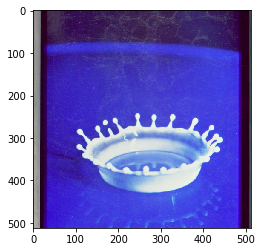
\includegraphics[width=0.15\textwidth]{opencv_files/output_5_1.png}


\subsection{Scaling and Rotation}\label{scaling-and-rotation}

Scaling (resizing) the image relative to different axis

\begin{verbatim}
res = cv2.resize(img,
                 None,
                 fx=1.2, 
                 fy=0.7, 
                 interpolation=cv2.INTER_CUBIC)
plt.imshow(res)
\end{verbatim}

which results in 

\includegraphics[width=0.15\textwidth]{opencv_files/output_7_1.png}


Rotation of the image for an angle of t

\begin{verbatim}
rows,cols,_ = img.shape
t = 45
M = cv2.getRotationMatrix2D((cols/2,rows/2),t,1)
dst = cv2.warpAffine(img,M,(cols,rows))

plt.imshow(dst)
\end{verbatim}

which results in 

\includegraphics[width=0.15\textwidth]{opencv_files/output_9_1.png}

\subsection{Gray-scaling}\label{gray-scaling}

\begin{verbatim}
img2 = cv2.cvtColor(img, cv2.COLOR_BGR2GRAY)
plt.imshow(img2, cmap='gray')
\end{verbatim}

which results in 

\includegraphics[width=0.15\textwidth]{opencv_files/output_11_1.png}


\subsection{Image Thresholding}\label{image-thresholding}

\begin{verbatim}
ret,thresh =    cv2.threshold(img2,127,255,cv2.THRESH_BINARY)
plt.subplot(1,2,1), plt.imshow(img2, cmap='gray')
plt.subplot(1,2,2), plt.imshow(thresh, cmap='gray')
\end{verbatim}

which results in 

\includegraphics[width=0.3\textwidth]{opencv_files/output_13_1.png}


\subsection{Edge Detection}\label{edge-detection}

Edge detection using Canny edge detection algorithm

\begin{verbatim}
edges = cv2.Canny(img2,100,200)

plt.subplot(121),plt.imshow(img2,cmap = 'gray')
plt.subplot(122),plt.imshow(edges,cmap = 'gray')
\end{verbatim}

which results in 

\includegraphics[width=0.3\textwidth]{opencv_files/output_15_1.png}


\section{Additional Features}

OpenCV has implementations of many machine learning techniques such as
KMeans and Support Vector Machines, that can be put into use with only
a few lines of code. It also has functions especially for video
analysis, feature detection, object recognition and many more. You can
find out more about them in their website

\URL{https://docs.opencv.org/3.0-beta/index.html}

OpenCV was initially developed for C++ and still has a focus on that
language, but it is still one of the most valuable image processing
libraries in Python.

\newpage
\section{Secchi Disk}\label{c:secchi-disk}

\subsection{Overview}\label{overview}

More information about Secchi DIsk can be found at:

  \URL{https://en.wikipedia.org/wiki/Secchi/_disk}

\begin{figure}[htb]
\centering
\includegraphics[height=0.25\textheight]{secchi/disk.png}
\caption{secchi}
\end{figure}

Figure: Different kinds of Secchi disks. A marine style on the left and
the freshwater version on the right {[}wikipedia{]}

\section{Setup for OSX}\label{setup-for-osx}

First lest setup the environment for OSX

\begin{verbatim}
import os, sys
from os.path import expanduser
os.path
home = expanduser("~")
sys.path.append('/usr/local/Cellar/opencv/3.3.1_1/lib/python3.6/site-packages/')
sys.path.append(home + '/.pyenv/versions/OPENCV/lib/python3.6/site-packages/')
import cv2
cv2.__version__
! pip install numpy > tmp.log
! pip install matplotlib >> tmp.log
%matplotlib inline
\end{verbatim}

\subsection{Step 1: Record the video}\label{step-1-record-the-video}

Record the video on the robot

\subsection{Step 2: Analyse the images from the
Video}\label{step-2-analyse-the-images-from-the-video}

For now we just selected 4 images from the video

\begin{verbatim}
import cv2
import matplotlib.pyplot as plt

img1 = cv2.imread('secchi/secchi1.png') 
img2 = cv2.imread('secchi/secchi2.png') 
img3 = cv2.imread('secchi/secchi3.png') 
img4 = cv2.imread('secchi/secchi4.png') 
\end{verbatim}

\begin{verbatim}
figures = []
fig = plt.figure(figsize=(18, 16))
for i in range(1,13):
    figures.append(fig.add_subplot(4,3,i))
count = 0
for img in [img1,img2,img3,img4]:
    figures[count].imshow(img)

    color = ('b','g','r')
    for i,col in enumerate(color):
        histr = cv2.calcHist([img],[i],None,[256],[0,256])
        figures[count+1].plot(histr,color = col)

    figures[count+2].hist(img.ravel(),256,[0,256])

    count += 3

print("Legend")
print("First column = image of Secchi disk")
print("Second column = histogram of colors in image")
print("Third column = histogram of all values")

plt.show() 
\end{verbatim}

\includegraphics[width=1.0\textwidth]{secchi-a/output_9_1.png}

Rotation of the image for an angle of t

\subsubsection{Image Thresholding}\label{image-thresholding}

\begin{verbatim}
def threshold(img):
    ret,thresh = cv2.threshold(img,150,255,cv2.THRESH_BINARY)
    plt.subplot(1,2,1), plt.imshow(img, cmap='gray')
    plt.subplot(1,2,2), plt.imshow(thresh, cmap='gray')
\end{verbatim}

\begin{verbatim}
threshold(img1)
\end{verbatim}

\includegraphics{secchi-a/output_13_0.png}


\begin{verbatim}
threshold(img2)
\end{verbatim}

\includegraphics{secchi-a/output_14_0.png}

\begin{verbatim}
threshold(img3)
\end{verbatim}

\includegraphics{secchi-a/output_15_0.png}

\begin{verbatim}
threshold(img4)
\end{verbatim}

\includegraphics{secchi-a/output_16_0.png}

\subsubsection{Edge Detection}\label{edge-detection}

Edge detection using Canny edge detection algorithm

\begin{verbatim}
def find_edge(img):
    edges = cv2.Canny(img,50,200)
    plt.subplot(121),plt.imshow(img,cmap = 'gray')
    plt.subplot(122),plt.imshow(edges,cmap = 'gray')
\end{verbatim}

\begin{verbatim}
find_edge(img1)
\end{verbatim}

\includegraphics{secchi-a/output_19_0.png}

\begin{verbatim}
find_edge(img2)
\end{verbatim}

\includegraphics{secchi-a/output_20_0.png}

\begin{verbatim}
find_edge(img3)
\end{verbatim}

\includegraphics{secchi-a/output_21_0.png}

\begin{verbatim}
find_edge(img4)
\end{verbatim}

\includegraphics{secchi-a/output_22_0.png}

\section{Black and white}\label{black-and-white}

\begin{verbatim}
bw1 = cv2.cvtColor(img1, cv2.COLOR_BGR2GRAY)
plt.imshow(bw1, cmap='gray')
\end{verbatim}

\includegraphics[width=0.5\textwidth]{secchi-a/output_26_1.png}

\chapter{Scipy}
\label{c:scipy}

SciPy is a library built above numpy and has a number of off the shelf
algorithms and operations implemented. These include algorithms from
calculus (such as integration), statistics, linear algebra,
image-processing, signal processing, machine learning.

To achieve this, SciPy bundels a number of useful open-source software
for mathematics, science, and engineering. It includes the follwoing
packages:

\begin{description}

\item[NumPy,] for managin N-dimensional arrays
\item[SciPy library,] to access fundamental scientific computing capabilities
\iten[Matplotlib,] to conduct 2D plotting
\item[IPython,] for an Interactive console (see jupyter)
\item[Sympy,] for symbolic mathematics
\item[pandas,] for providing data structures and analysis

\end{description}


\section{Introduction}

First we add the usual scientific computing modules with the typical
abbreviations, including sp for scipy. We could invoke scipy's
statistical package as sp.stats, but for the sake of laziness we
abbreviate that too.

\begin{verbatim}
import numpy as np # import numpy
import scipy as sp # import scipy
from scipy import stats # refer directly to stats rather than sp.stats
import matplotlib as mpl # for visualization
from matplotlib import pyplot as plt # refer directly to pyplot 
                                     # rather than mpl.pyplot
\end{verbatim}

Now we create some random data to play with. We generate 100 samples
from a Gaussian distribution centered at zero.

\begin{verbatim}
s = sp.randn(100)
\end{verbatim}

How many elements are in the set?

\begin{verbatim}
print ('There are',len(s),'elements in the set')
\end{verbatim}

What is the mean (average) of the set?

\begin{verbatim}
print ('The mean of the set is',s.mean())
\end{verbatim}

What is the minimum of the set?

\begin{verbatim}
print ('The minimum of the set is',s.min())
\end{verbatim}

What is the maximum of the set?

\begin{verbatim}
print ('The maximum of the set is',s.max())
\end{verbatim}

We can use the scipy functions too. What's the median?

\begin{verbatim}
print ('The median of the set is',sp.median(s))
\end{verbatim}

What about the standard deviation and variance?

\begin{verbatim}
print ('The standard deviation is',sp.std(s),
       'and the variance is',sp.var(s))
\end{verbatim}

Isn't the variance the square of the standard deviation?

\begin{verbatim}
print ('The square of the standard deviation is',sp.std(s)**2)
\end{verbatim}

How close are the measures? The differences are close as the following
calculation shows

\begin{verbatim}
print ('The difference is',abs(sp.std(s)**2 - sp.var(s)))
\end{verbatim}

\begin{verbatim}
print ('And in decimal form, the difference is %0.16f' % 
       (abs(sp.std(s)**2 - sp.var(s))))
\end{verbatim}

How does this look as a histogram?

\begin{verbatim}
plt.hist(s) # yes, one line of code for a histogram
plt.show()
\end{verbatim}

\begin{center}
\includegraphics[width=0.5\textwidth]{scipy/output_23_0.png}
\end{center}

Let's add some titles.

\begin{verbatim}
plt.clf() # clear out the previous plot

plt.hist(s)
plt.title("Histogram Example")
plt.xlabel("Value")
plt.ylabel("Frequency")

plt.show()
\end{verbatim}

\begin{center}
\includegraphics[width=0.5\textwidth]{scipy/output_25_0.png}
\end{center}

Typically we do not include titles when we prepare images for inclusion
in LaTeX. There we use the caption to describe what the figure is about.

\begin{verbatim}
plt.clf() # clear out the previous plot

plt.hist(s)
plt.xlabel("Value")
plt.ylabel("Frequency")

plt.show()
\end{verbatim}

\begin{center}
\includegraphics[width=0.5\textwidth]{scipy/output_27_0.png}
\end{center}

Let's try out some linear regression, or curve fitting.

\begin{verbatim}
import random

def F(x):
    return 2*x - 2

def add_noise(x):
    return x + random.uniform(-1,1) 
\end{verbatim}

\begin{verbatim}
X = range(0,10,1)

Y = []
for i in range(len(X)):
    Y.append(add_noise(X[i]))

plt.clf() # clear out the old figure
plt.plot(X,Y,'.')
plt.show()
\end{verbatim}

\begin{center}
\includegraphics[width=0.5\textwidth]{scipy/output_30_0.png}
\end{center}

Now let's try linear regression to fit the curve.

\begin{verbatim}
m, b, r, p, est_std_err = stats.linregress(X,Y)
\end{verbatim}

What is the slope and y-intercept of the fitted curve?

\begin{verbatim}
print ('The slope is',m,'and the y-intercept is', b)
\end{verbatim}

\begin{verbatim}
def Fprime(x): # the fitted curve
    return m*x + b
\end{verbatim}

Now let's see how well the curve fits the data. We'll call the fitted
curve F'.

\begin{verbatim}
X = range(0,10,1)

Yprime = []
for i in range(len(X)):
    Yprime.append(Fprime(X[i]))
\end{verbatim}

\begin{verbatim}
plt.clf() # clear out the old figure

# the observed points, blue dots
plt.plot(X, Y, '.', label='observed points') 

# the interpolated curve, connected red line
plt.plot(X, Yprime, 'r-', label='estimated points')  

plt.title("Linear Regression Example") # title
plt.xlabel("x") # horizontal axis title
plt.ylabel("y") # vertical axis title
# legend labels to plot
plt.legend(['obsered points', 'estimated points']) 

# comment out so that you can save the figure
#plt.show()
\end{verbatim}

To save images into a PDF file for inclusion into \LaTeX documents you
can save the images as follows. Other formats such as png are also
possible, but the quality is naturally not sufficient for inclusion in
papers and documents. For that you certainly want to use PDF. The save
of the figure has to occure before you use the \verb|show()| command.

\begin{verbatim}
plt.savefig("regression.pdf", bbox_inches='tight')
\end{verbatim}

\begin{verbatim}
plt.savefig('regression.png') 
\end{verbatim}

\begin{verbatim}
plt.show()
\end{verbatim}

\begin{center}
\includegraphics[width=0.5\textwidth]{scipy/output_40_0.png}
\end{center}


\section{References}\label{references}

For more information about SciPy we recommend that you visit the following link

\URL{https://www.scipy.org/getting-started.html#learning-to-work-with-scipy}

Additional material and inspiration for this section are from

\begin{itemize}
\item ``Getting Started guide'' \url{https://www.scipy.org/getting-started.html}
\item
  Prasanth. ``Simple statistics with SciPy.'' Comfort at 1 AU. 
  February 28, 2011.   \url{https://oneau.wordpress.com/2011/02/28/simple-statistics-with-scipy/}.
\item
  SciPy Cookbook. Lasted updated: 2015. 
  \url{http://scipy-cookbook.readthedocs.io/}. 
\end{itemize}

\chapter{Numpy}\label{c:numpy}

NumPy is a popular library on that is used by many other python
librariessuch as pandas, and SciPy. It provides simple to use array
operations for data. This helps to accass arrays in a more intuitive
fashion and introduces various matrix operations.

We provide a short introduction to Numpy.

First we import the modules needed for this introduction and abreviate
them with the \texttt{as} feature of the import statement

\begin{verbatim}
import numpy as np
import matplotlib as mpl
import matplotlib.pyplot as plt
\end{verbatim}

Now we showcase some features of Numpy.

\section{Float Range}\label{float-range}

\texttt{arange()} is like \texttt{range()}, but for floating-point
numbers.

\begin{verbatim}
X = np.arange(0.2,1,.1)
\end{verbatim}

\begin{verbatim}
print (X)
\end{verbatim}

We use this function to generate parameter space that can then be
iterated on.

\begin{verbatim}
P = 10.0 ** np.arange(-7,1,1)

print (P)
\end{verbatim}

\begin{verbatim}
for x,p in zip(X,P):
    print ('%f, %f' % (x, p))
\end{verbatim}

\section{Arrays}\label{arrays}

To create one dimensional arrays you use

\begin{verbatim}
a = np.array([1, 2, 3])   
\end{verbatim}

To check some properties you can use the following

\begin{verbatim}
print(type(a))            # Prints "<class 'numpy.ndarray'>"
\end{verbatim}

\begin{verbatim}
print(a.shape)            # Prints "(3,)"
\end{verbatim}

The shape indicates that in the first dimension, there are 3 elements.
To print the actual values you can use

\begin{verbatim}
print(a)                  # Prints the values of the array
print(a[0], a[1], a[2])   # Prints "1 2 3"
\end{verbatim}

To change values you can use the index of the element or use any other
python method to do so. IN our example we change the first element to
\texttt{42}

\begin{verbatim}
a[0] = 42                 
print(a)                  
\end{verbatim}

To create more dimensional arrays you use

\begin{verbatim}
b = np.array([[1,2,3],[4,5,6]])    # Create a 2 dimensional array
print(b.shape)                     # Prints "(2, 3)"
print(b[0, 0], b[0, 1], b[1, 0])   # Prints "1 2 4"
\end{verbatim}

\section{Array Operations}\label{array-operations}

Let us first create some arrays with a predefined datatype

\begin{verbatim}
x = np.array([[1,2],[3,4]], dtype=np.float64)
y = np.array([[5,6],[7,8]], dtype=np.float64)
\end{verbatim}

\begin{verbatim}
print (x)
\end{verbatim}

\begin{verbatim}
print(y)
\end{verbatim}

To add the numbers use

\begin{verbatim}
print(x+y)
\end{verbatim}

Other functions such as \texttt{-}, \texttt{*}, \texttt{/} behave as
expected using elementwise oerations:

\begin{verbatim}
print(x-y)
\end{verbatim}

\begin{verbatim}
print(x*y)
\end{verbatim}

\begin{verbatim}
print(x/y)
\end{verbatim}

To apply functions such as `sin' make sure you use the function provided
by the numpy package such as \texttt{np.sin}. The list of functions is
included in the manual at *
\url{https://docs.scipy.org/doc/numpy/reference/routines.math.html}

\begin{verbatim}
print (np.sin(x))
\end{verbatim}

\begin{verbatim}
print (np.sum(x))
\end{verbatim}

Computations can also be applied to columns and rows

\begin{verbatim}
print(np.sum(x, axis=0)) # sum of each column
print(np.sum(x, axis=1)) # sum of each row
\end{verbatim}

\section{Linear Algebra}\label{linear-algebra}

Linear algebra methods are also provided.

\begin{verbatim}
from numpy import linalg 

A = np.diag((1,2,3))

w,v = linalg.eig(A)

print ('w =', w)
print ('v =', v)
\end{verbatim}

\section{Resources}\label{resources}

\begin{itemize}
\tightlist
\item
  \url{https://docs.scipy.org/doc/numpy/}
\item
  \url{http://cs231n.github.io/python-numpy-tutorial/\#numpy}
\end{itemize}




\part{Python Cloudmesh}

\chapter{Cloudmesh}

In this chapter we will be using some advanced Python features to
enhance Cloudmesh that is supposed to easily manage multiple
clouds. We will be explicitly using python 3 and do
not worry about backwards compatibility.

We will be developing it as community so that new features can be
integrated and loaded on demand while adding an extensible package
management system based on pythons shared namespace. To do so we will
rely on \verb|cmd5| that includes a generate command to add new
papackes on demand. We will not use all features of cmd5.

We are trying to develop the following:

\begin{description}

\item[Configuration] so that we can easily configure and add various
  clouds to our multi-cloud environment.

\item[Database] of virtual machines and clouds so that they can be
  managed across different clouds in a multi cloud environment

\item[API Classes] so that we can use python as a convenient
  programming environment.

\item[Context] libraries so taht in python we can easily apply context
  for clouds and virtual machines on a block of statements

\item[Command Shell] so that we can similar to matlab
  and other shells execute multiple commands

\item[REST Services]  so that we can access the features
form other programming environments and different programming
languages.

\item[Parallel Services] so that we can issue commands in parallel and
  manage virtual machines in a multi cloud environment.

\end{description}



\section{Configuration}

As we are developing a multi-cloud environment, we need some mechanism
to define the clouds easily. To make our development effort simpler,
we like to point out that the configuration file must be stored in a
particular location relative to the home directory. We store the file
in \verb|~/.cloudmesh/class.yaml|. Additionally we store our cloud
passwords in this file in cleartext and thus we must make sure our
machine is not compromized and that we properly protect the file. On a
unix system you do this with:

\begin{verbatim}
mkdir ~/.cloudmesh
touch ~/.cloudmesh/class.yaml
chmod go-rw ~/.cloudmesh
chmod go-rw ~/.cloudmesh/class.yaml
\end{verbatim}

In that directory we store a file similar to the following file:

\begin{verbatim}
version: 5.0
profile:
  firstname: Gregor
  lastname: von Laszewski
  email: laszewski@gmail.com
cloudmesh:
  default:
  - chameleon 
  active:
  - chameleon
clouds:
  uc:
    name: Chameleon UC
    host: chameleoncloud.org
    type: openstack
    version: liberty
    credentials:
      OS_AUTH_URL: https://openstack.uc.chameleoncloud.org:5000/v3
      OS_PASSWORD: TBD
      OS_TENANT_NAME: CH-818664
      OS_TENANT_ID: CH-818664
      OS_PROJECT_NAME: CH-818664
      OS_PROJECT_DOMAIN_ID: default
      OS_USER_DOMAIN_ID: default
      OS_USERNAME: TBD
      OS_VERSION: liberty
      OS_REGION_NAME: RegionOne
    default:
      flavor: m1.small
      image: Ubuntu-Server-14.04-LTS
  tacc:
    name: Chameleon TACC
    host: chameleoncloud.org
    type: openstack
    version: liberty
    credentials:
      OS_AUTH_URL: https://openstack.tacc.chameleoncloud.org:5000/v3
      OS_PASSWORD: TBD
      OS_TENANT_NAME: CH-818664
      OS_TENANT_ID: CH-818664
      OS_PROJECT_NAME: CH-818664
      OS_PROJECT_DOMAIN_ID: default
      OS_USER_DOMAIN_ID: default
      OS_USERNAME: TBD
      OS_VERSION: liberty
      OS_REGION_NAME: RegionOne
    default:
      flavor: m1.small
      image: Ubuntu-Server-14.04-LTS
\end{verbatim}

Important to note is that this file defines multiple clouds and uses
the attribute value TBD for password and username which you may want
to change. However, we also would like to support a mode that when the
password is defined to be TBD that it is asked from the terminal. This
way we do not necessarily have to store the password here. In future
we will enhance this file to be encrypted and decrypted with a
password protected ssh key.

The file is ayaml file as the typical configuration in python is not
suitable to easily store hierarchical data. YAML is also more readable
than json so it provides a really good way of defining the
configuration data. Problematic with yaml readers however are that
they typically do not preserver the read order. Your task will be to
write a \textit{short} yaml configuration reader that preserves the
order. You are encouraged to reuse methods. What your are not supposed
to do is to reimplement yaml.

There are some special properties of this file that we need to
discuss. 

\begin{itemize}

\item clouds are listed in the clouds section
\item the credentials section to each cloud defines how to connect to
  the cloud with python libraries such as libcloud. Each cloud type will
  have different parameters.
\item 


\end{itemize}



\section{Storage}

As we need to store some of the data we must identify a suitable
database for storing information about virtual machines and other
information related to the clouds. Although shelve comes in mind, we
found out that it is not compatible between python 2 and 3 which may
be an issue in future. Also when considering services such as mongodb
they have to be started and properly secured. THis naturally can be
done with containers. We also do not want to use large frameworks such
as django which come with build in object models as they are not
lightwight. Hence, we start we just use a file based sql
database as provided with sqlite3.

\subsection{sqlite3}

While we keep the configuration in the configuration yaml file we
intend to create a database entry for virtual machines we start in the
cloud. In order to store hierarchical information that we may obtain
in dict format from a virtual machine we can easily create flattened
out data structures, by simple connecting the attribute names and
separate them by \verb|_|.

Let us assome we want to store an object of the following form:

\begin{verbatim}
element = {
   'id': 1,
   'cloud': 'chameleon',
   'name': 'vm1',
   'data': {
       "image": 'ubuntu',
       "flavor": "small"
    }
}
\end{verbatim}

A table that could store such an object could be

\begin{verbatim}
create table element (
    id           integer primary key,
    name         text
    cloud        text,
    data_image:  text,
    data_flavor: text
);
\end{verbatim}

Obviously, we could create the table automatically from recursively
iterating through the dict to make our approach generalized for any
dict. As for the primary key, we simply assume it is always the id
which is an integer that always increases and is stored in the database.
as a separate element.

Thus we probably want a table generator such as

\begin{lstlisting}{python}
class Database (object):
   @staticmethod
   def generate (dictionary):
      # implement me
\end{lstlisting}

Additionally we want to create convenience methods for adding,
deleting, and searching information


\subsection{Context}

Python provides the feature of a context that we are well familiar
with from file management. An example is:

\begin{lstlisting}{python}
with open('/tmp/gregor.txt', 'wt') as f:
    f.write('Hello Gregor')
# after this, the file is automatically closed
\end{lstlisting}

If we look at this example it is desirable to develop at least two
context for multicloud envireonments. The first is to manage virtual
machines on named clouds and issue action on it, such as \textit{start, stop,
  suspend, resume, delete}. In the other context we like to issue
such asction on named virtual machines.

To illustrate what we have in mind, please take a look at our initial
examples.

\subsubsection{Cloud Context}

When defining the following cloud context 

\begin{lstlisting}{python}
class Cloud (object):
    
    def __init__(self, name):
        self.name = name

    def __enter__(self):
        print ('Running on:', self.name)
        return self

    def __exit__(self, exc_type, exc_val, exc_tb):
        print('__exit__()')

    def machine(self, name, action):
        print (name, action)
\end{lstlisting}

we can issue conveniently commands such as the following 

\begin{lstlisting}{python}
cloud = 'chameleon'
with Cloud(cloud) as c:
    vm = c.machine('vm1', 'start')
\end{lstlisting}

It is obvious that through this abstraction we can formulate a
tempalted bahavior such as starting a virtual machine and through the
switch of a ingle variable (\verb|cloud|) issue the command on other
clouds.






%\part{Python Notebooks}

%\section{NIST Pedestrian and Face
Detection}\label{nist-pedestrian-and-face-detection}

Pedestrian and Face Detection uses OpenCV to identify people standing in
a picture or a video and NIST use case in this document is built with
Apache Spark and Mesos clusters on multiple compute nodes.

The example in this tutorial deploys software packages on OpenStack
using Ansible with its roles.

\begin{longtable}[]{@{}ll@{}}
\toprule
\begin{minipage}[b]{0.20\columnwidth}\raggedright\strut
Original\strut
\end{minipage} & \begin{minipage}[b]{0.31\columnwidth}\raggedright\strut
Pedestrian Detected\strut
\end{minipage}\tabularnewline
\midrule
\endhead
\begin{minipage}[t]{0.20\columnwidth}\raggedright\strut
\includegraphics{https://raw.githubusercontent.com/cloudmesh/classes/master/docs/source/notebooks/files/image03.png}\strut
\end{minipage} & \begin{minipage}[t]{0.31\columnwidth}\raggedright\strut
\includegraphics{https://raw.githubusercontent.com/cloudmesh/classes/master/docs/source/notebooks/files/image05.png}\strut
\end{minipage}\tabularnewline
\bottomrule
\end{longtable}

\begin{longtable}[]{@{}ll@{}}
\toprule
\begin{minipage}[b]{0.22\columnwidth}\raggedright\strut
Original\strut
\end{minipage} & \begin{minipage}[b]{0.50\columnwidth}\raggedright\strut
Pedestrian and Face/eyes Detected\strut
\end{minipage}\tabularnewline
\midrule
\endhead
\begin{minipage}[t]{0.22\columnwidth}\raggedright\strut
\includegraphics{https://raw.githubusercontent.com/cloudmesh/classes/master/docs/source/notebooks/files/image06.png}\strut
\end{minipage} & \begin{minipage}[t]{0.50\columnwidth}\raggedright\strut
\includegraphics{https://raw.githubusercontent.com/cloudmesh/classes/master/docs/source/notebooks/files/image04.png}\strut
\end{minipage}\tabularnewline
\bottomrule
\end{longtable}

\subsection{Introduction}\label{introduction}

Human (pedestrian) detection and face detection have been studied during
the last several years and models for them have improved along with
Histograms of Oriented Gradients (HOG) for Human Detection {[}1{]}.
OpenCV is a Computer Vision library including the SVM classifier and the
HOG object detector for pedestrian detection and INRIA Person Dataset
{[}2{]} is one of popular samples for both training and testing
purposes. In this document, we deploy Apache Spark on Mesos clusters to
train and apply detection models from OpenCV using Python API.

\subsubsection{INRIA Person Dataset}\label{inria-person-dataset}

This dataset contains positive and negative images for training and test
purposes with annotation files for upright persons in each image. 288
positive test images, 453 negative test images, 614 positive training
images and 1218 negative training images are included along with
normalized 64x128 pixel formats. 970MB dataset is available to download
{[}3{]}.

\subsubsection{HOG with SVM model}\label{hog-with-svm-model}

Histogram of Oriented Gradient (HOG) and Support Vector Machine (SVM)
are used as object detectors and classifiers and built-in python
libraries from OpenCV provide these models for human detection.

\subsubsection{Ansible Automation Tool}\label{ansible-automation-tool}

Ansible is a python tool to install/configure/manage software on
multiple machines with JSON files where system descriptions are defined.
There are reasons why we use Ansible:

\begin{itemize}
\tightlist
\item
  Expandable: Leverages Python (default) but modules can be written in
  any language
\item
  Agentless: no setup required on managed node
\item
  Security: Allows deployment from user space; uses ssh for
  authentication
\item
  Flexibility: only requires ssh access to privileged user
\item
  Transparency: YAML Based script files express the steps of installing
  and configuring software
\item
  Modularity: Single Ansible Role (should) contain all required commands
  and variables to deploy software package independently
\item
  Sharing and portability: roles are available from source (github,
  bitbucket, gitlab, etc) or the Ansible Galaxy portal
\end{itemize}

We use Ansible roles to install software packages for Humand and Face
Detection which requires to run OpenCV Python libraries on Apache Mesos
with a cluster configuration. Dataset is also downloaded from the web
using an ansible role.

\subsection{Deployment by Ansible}\label{deployment-by-ansible}

Ansible is to deploy applications and build clusters for
batch-processing large datasets towards target machines e.g. VM
instances on OpenStack and we use ansible roles with \emph{include}
directive to organize layers of big data software stacks (BDSS). Ansible
provides abstractions by Playbook Roles and reusability by Include
statements. We define X application in X Ansible Role, for example, and
use include statements to combine with other applications e.g. Y or Z.
The layers exist in sub directories (see below) to add modularity to
your Ansible deployment. For example, there are five roles used in this
example that are Apache Mesos in a scheduler layer, Apache Spark in a
processing layer, a OpenCV library in an application layer, INRIA Person
Dataset in a dataset layer and a python script for human and face
detection in an analytics layer. If you have an additional software
package to add, you can simply add a new role in a main ansible playbook
with \emph{include} directive. With this, your Ansible playbook
maintains simple but flexible to add more roles without having a large
single file which is getting difficult to read when it deploys more
applications on multiple layers. The main Ansible playbook runs Ansible
roles in order which look like:

\begin{verbatim}
---
include: sched/00-mesos.yml
include: proc/01-spark.yml
include: apps/02-opencv.yml
include: data/03-inria-dataset.yml
Include: anlys/04-human-face-detection.yml
\end{verbatim}

Directory names e.g. sched, proc, data, or anlys indicate BDSS layers
like: - sched: scheduler layer - proc: data processing layer - apps:
application layer - data: dataset layer - anlys: analytics layer and two
digits in the filename indicate an order of roles to be run.

\subsection{Cloudmesh for
Provisioning}\label{cloudmesh-for-provisioning}

It is assumed that virtual machines are created by cloudmesh, the cloud
management software. For example on OpenStack,

\texttt{cm\ cluster\ create\ -N=6}

command starts a set of virtual machine instances. The number of
machines and groups for clusters e.g. namenodes and datanodes are
defined in the Ansible inventory file, a list of target machines with
groups, which will be generated once machines are ready to use by
cloudmesh. Ansible roles install software and dataset on virtual
clusters after that stage.

\subsection{Roles Explained for
Installation}\label{roles-explained-for-installation}

Mesos role is installed first as a scheduler layer for masters and
slaves where mesos-master runs on the masters group and mesos-slave runs
on the slaves group. Apache Zookeeper is included in the mesos role
therefore mesos slaves find an elected mesos leader for the
coordination. Spark, as a data processing layer, provides two options
for distributed job processing, batch job processing via a cluster mode
and real-time processing via a client mode. The Mesos dispatcher runs on
a masters group to accept a batch job submission and Spark interactive
shell, which is the client mode, provides real-time processing on any
node in the cluster. Either way, Spark is installed later to detect a
master (leader) host for a job submission. Other roles for OpenCV, INRIA
Person Dataset and Human and Face Detection Python applications are
followed by.

The following software are expected in the stacks according to the
\href{https://github.com/futuresystems/pedestrian-and-face-detection}{github}:

\begin{itemize}
\tightlist
\item
  mesos cluster (master, worker)
\item
  spark (with dispatcher for mesos cluster mode)
\item
  openCV
\item
  zookeeper
\item
  INRIA Person Dataset
\item
  Detection Analytics in Python
\item
  {[}1{]} Dalal, Navneet, and Bill Triggs. ``Histograms of oriented
  gradients for human detection.'' 2005 IEEE Computer Society Conference
  on Computer Vision and Pattern Recognition (CVPR'05). Vol. 1. IEEE,

  2005. {[}pdf{]}
\item
  {[}2{]} \url{http://pascal.inrialpes.fr/data/human/}
\item
  {[}3{]}
  \url{ftp://ftp.inrialpes.fr/pub/lear/douze/data/INRIAPerson.tar}
\item
  {[}4{]} \url{https://docs.python.org/2/library/configparser.html}
\end{itemize}

\subsubsection{Server groups for Masters/Slaves by Ansible
inventory}\label{server-groups-for-mastersslaves-by-ansible-inventory}

We may separate compute nodes in two groups: masters and workers
therefore Mesos masters and zookeeper quorums manage job requests and
leaders and workers run actual tasks. Ansible needs group definitions in
their inventory therefore software installation associated with a proper
part can be completed.

Example of Ansible Inventory file (inventory.txt)

\begin{verbatim}
[masters]
10.0.5.67
10.0.5.68
10.0.5.69
[slaves]
10.0.5.70
10.0.5.71
10.0.5.72
\end{verbatim}

\subsection{Instructions for
Deployment}\label{instructions-for-deployment}

The following commands complete NIST Pedestrian and Face Detection
deployment on OpenStack.

\subsubsection{Cloning Pedestrian Detection Repository from
Github}\label{cloning-pedestrian-detection-repository-from-github}

Roles are included as submodules which require \texttt{-\/-recursive}
option to checkout them all.

\begin{verbatim}
!git clone --recursive https://github.com/futuresystems/pedestrian-and-face-detection.git
\end{verbatim}

Change the following variable with actual ip addresses:

\begin{verbatim}
sample_inventory="""[masters]
10.0.5.67
10.0.5.68
10.0.5.69
[slaves]
10.0.5.70
10.0.5.71
10.0.5.72"""
\end{verbatim}

Create a \texttt{inventory.txt} file with the variable in your local
directory.

\begin{verbatim}
!printf "$sample_inventory" > inventory.txt
!cat inventory.txt
\end{verbatim}

Add \texttt{ansible.cfg} file with options for ssh host key checking and
login name.

\begin{verbatim}
ansible_config="""[defaults]
host_key_checking=false
remote_user=ubuntu"""
!printf "$ansible_config" > ansible.cfg
!cat ansible.cfg
\end{verbatim}

Check accessibility by ansible ping like:

\begin{verbatim}
!ansible -m ping -i inventory.txt all
\end{verbatim}

Make sure that you have a correct ssh key in your account otherwise you
may encounter `FAILURE' in the ping test above.

\subsubsection{Ansible Playbook}\label{ansible-playbook}

We use a main ansible playbook to deploy software packages for NIST
Pedestrian and Face detection which includes: - mesos - spark -zookeeper
- opencv - INRIA Person dataset - Python script for the detection

\begin{verbatim}
!cd pedestrian-and-face-detection/ && ansible-playbook -i ../inventory.txt site.yml
\end{verbatim}

The installation may take 30 minutes or an hour to complete.

\subsection{OpenCV in Python}\label{opencv-in-python}

Before we run our code for this project, let's try OpenCV first to see
how it works.

\subsubsection{Import cv2}\label{import-cv2}

Let's import opencv python module and we will use images from the online
database image-net.org to test OpenCV image recognition.

\begin{verbatim}
import cv2
\end{verbatim}

Let's download a mailbox image with a red color to see if opencv
identifies the shape with a color. The example file in this tutorial is:

\begin{verbatim}
!curl http://farm4.static.flickr.com/3061/2739199963_ee78af76ef.jpg > mailbox.jpg
\end{verbatim}

\begin{quote}
100 167k 100 167k 0 0 686k 0 --:--:-- --:--:-- --:--:-- 684k
\end{quote}

\begin{verbatim}
%matplotlib inline
\end{verbatim}

\begin{verbatim}
from IPython.display import Image
mailbox_image = "mailbox.jpg"
Image(filename=mailbox_image)
\end{verbatim}

\includegraphics{facedetection_files/facedetection_46_0.jpeg}

You can try other images. Check out the image-net.org for mailbox
images: \url{http://image-net.org/synset?wnid=n03710193}

\subsubsection{Image Detection}\label{image-detection}

Just for a test, let's try to detect a red color shaped mailbox using
opencv python functions.

There are key functions that we use: * cvtColor: to convert a color
space of an image * inRange: to detect a mailbox based on the range of
red color pixel values * np.array: to define the range of red color
using a Numpy library for better calculation * findContours: to find a
outline of the object * bitwise\_and: to black-out the area of contours
found

\begin{verbatim}
import numpy as np
import matplotlib.pyplot as plt

# imread for loading an image
img = cv2.imread(mailbox_image)
# cvtColor for color conversion
hsv = cv2.cvtColor(img,cv2.COLOR_BGR2HSV)

# define range of red color in hsv
lower_red1 = np.array([0, 50, 50])
upper_red1 = np.array([10, 255, 255])
lower_red2 = np.array([170, 50, 50])
upper_red2 = np.array([180, 255, 255])

# threshold the hsv image to get only red colors
mask1 = cv2.inRange(hsv, lower_red1, upper_red1)
mask2 = cv2.inRange(hsv, lower_red2, upper_red2)
mask = mask1 + mask2

# find a red color mailbox from the image
im2, contours,hierarchy = cv2.findContours(mask, cv2.RETR_TREE, cv2.CHAIN_APPROX_SIMPLE)

# bitwise_and to remove other areas in the image except the detected object
res = cv2.bitwise_and(img, img, mask = mask)

# turn off - x, y axis bar
plt.axis("off")
# text for the masked image
cv2.putText(res, "masked image", (20,300), cv2.FONT_HERSHEY_SIMPLEX, 2, (255,255,255))
# display
plt.imshow(cv2.cvtColor(res, cv2.COLOR_BGR2RGB))
plt.show()
\end{verbatim}

\includegraphics{facedetection_files/facedetection_49_0.png}

The red color mailbox is left alone in the image which we wanted to find
in this example by opencv functions. You can try other images with
different colors to detect the different shape of objects using
findContours and inRange from opencv.

For more information, see the useful links below.

\begin{itemize}
\tightlist
\item
  contours features:
  \url{http://docs.opencv.org/3.1.0/dd/d49/tutorial/_py/_contour/_features.html}
\item
  contours:
  \url{http://docs.opencv.org/3.1.0/d4/d73/tutorial/_py/_contours/_begin.html}
\item
  red color in hsv:
  \url{http://stackoverflow.com/questions/30331944/finding-red-color-using-python-opencv}
\item
  inrange:
  \url{http://docs.opencv.org/master/da/d97/tutorial/_threshold/_inRange.html}
\item
  inrange:
  \url{http://docs.opencv.org/3.0-beta/doc/py/_tutorials/py/_imgproc/py/_colorspaces/py/_colorspaces.html}
\item
  numpy:
  \url{http://docs.opencv.org/3.0-beta/doc/py/_tutorials/py/_core/py/_basic/_ops/py/_basic/_ops.html}
\end{itemize}

\subsection{Human and Face Detection in
OpenCV}\label{human-and-face-detection-in-opencv}

\subsubsection{INRIA Person Dataset}\label{inria-person-dataset-1}

We use INRIA Person dataset to detect upright people and faces in images
in this example. Let's download it first.

\begin{verbatim}
!curl ftp://ftp.inrialpes.fr/pub/lear/douze/data/INRIAPerson.tar > INRIAPerson.tar
\end{verbatim}

\begin{quote}
100 969M 100 969M 0 0 8480k 0 0:01:57 0:01:57 --:--:-- 12.4M
\end{quote}

\begin{verbatim}
!tar xvf INRIAPerson.tar > logfile && tail logfile
\end{verbatim}

\subsubsection{Face Detection using Haar
Cascades}\label{face-detection-using-haar-cascades}

This section is prepared based on the opencv-python tutorial:
\url{http://docs.opencv.org/3.1.0/d7/d8b/tutorial/_py/_face/_detection.html\#gsc.tab=0}

There is a pre-trained classifier for face detection, download it from
here:

\begin{verbatim}
!curl https://raw.githubusercontent.com/opencv/opencv/master/data/haarcascades/haarcascade_frontalface_default.xml > haarcascade_frontalface_default.xml
\end{verbatim}

\begin{quote}
100 908k 100 908k 0 0 2225k 0 --:--:-- --:--:-- --:--:-- 2259k
\end{quote}

This classifier XML file will be used to detect faces in images. If you
like to create a new classifier, find out more information about
training from here:
\url{http://docs.opencv.org/3.1.0/dc/d88/tutorial/_traincascade.html}

\subsubsection{Face Detection Python Code
Snippet}\label{face-detection-python-code-snippet}

Now, we detect faces from the first five images using the classifier.

\begin{verbatim}
# import the necessary packages
from __future__ import print_function
import numpy as np
import cv2
from os import listdir
from os.path import isfile, join
import matplotlib.pyplot as plt

mypath = "INRIAPerson/Test/pos/"
face_cascade = cv2.CascadeClassifier('haarcascade_frontalface_default.xml')

onlyfiles = [join(mypath, f) for f in listdir(mypath) if isfile(join(mypath, f))]

cnt = 0
for filename in onlyfiles:
    image = cv2.imread(filename)
    image_grayscale = cv2.cvtColor(image, cv2.COLOR_BGR2GRAY)
    faces = face_cascade.detectMultiScale(image_grayscale, 1.3, 5)
    if len(faces) == 0:
        continue

    cnt_faces = 1
    for (x,y,w,h) in faces:
        cv2.rectangle(image,(x,y),(x+w,y+h),(255,0,0),2)
        cv2.putText(image, "face" + str(cnt_faces), (x,y-10), cv2.FONT_HERSHEY_SIMPLEX, 1, (0,0,0), 2)
        plt.figure()
        plt.axis("off")
        plt.imshow(cv2.cvtColor(image[y:y+h, x:x+w], cv2.COLOR_BGR2RGB))
        cnt_faces += 1
    plt.figure()
    plt.axis("off")
    plt.imshow(cv2.cvtColor(image, cv2.COLOR_BGR2RGB))        
    cnt = cnt + 1
    if cnt == 5:
        break
\end{verbatim}

\includegraphics{facedetection_files/facedetection_59_0.png}

\includegraphics{facedetection_files/facedetection_59_1.png}

\includegraphics{facedetection_files/facedetection_59_2.png}

\includegraphics{facedetection_files/facedetection_59_3.png}

\includegraphics{facedetection_files/facedetection_59_4.png}

\includegraphics{facedetection_files/facedetection_59_5.png}

\includegraphics{facedetection_files/facedetection_59_6.png}

\includegraphics{facedetection_files/facedetection_59_7.png}

\includegraphics{facedetection_files/facedetection_59_8.png}

\includegraphics{facedetection_files/facedetection_59_9.png}

\includegraphics{facedetection_files/facedetection_59_10.png}

\subsection{Pedestrian Detection using HOG
Descriptor}\label{pedestrian-detection-using-hog-descriptor}

We will use Histogram of Oriented Gradients (HOG) to detect a upright
person from images.

\subsubsection{Python Code Snippet}\label{python-code-snippet}

\begin{verbatim}
# initialize the HOG descriptor/person detector
hog = cv2.HOGDescriptor()
hog.setSVMDetector(cv2.HOGDescriptor_getDefaultPeopleDetector())

cnt = 0
for filename in onlyfiles:
    img = cv2.imread(filename)
    orig = img.copy()
    gray = cv2.cvtColor(img, cv2.COLOR_BGR2GRAY)

    # detect people in the image
    (rects, weights) = hog.detectMultiScale(img, winStride=(8, 8),
    padding=(16, 16), scale=1.05)

    # draw the final bounding boxes
    for (x, y, w, h) in rects:
        cv2.rectangle(img, (x, y), (x + w, y + h), (0, 255, 0), 2)

    plt.figure()
    plt.axis("off")
    plt.imshow(cv2.cvtColor(orig, cv2.COLOR_BGR2RGB))
    plt.figure()
    plt.axis("off")
    plt.imshow(cv2.cvtColor(img, cv2.COLOR_BGR2RGB))
    cnt = cnt + 1
    if cnt == 5:
        break
\end{verbatim}

\includegraphics{facedetection_files/facedetection_62_0.png}

\includegraphics{facedetection_files/facedetection_62_1.png}

\includegraphics{facedetection_files/facedetection_62_2.png}

\includegraphics{facedetection_files/facedetection_62_3.png}

\includegraphics{facedetection_files/facedetection_62_4.png}

\includegraphics{facedetection_files/facedetection_62_5.png}

\includegraphics{facedetection_files/facedetection_62_6.png}

\includegraphics{facedetection_files/facedetection_62_7.png}

\includegraphics{facedetection_files/facedetection_62_8.png}

\includegraphics{facedetection_files/facedetection_62_9.png}

\subsection{Processing by Apache
Spark}\label{processing-by-apache-spark}

INRIA Person dataset provides 100+ images and Spark can be used for
image processing in parallel. We load 288 images from ``Test/pos''
directory.

Spark provides a special object `sc' to connect between a spark cluster
and functions in python code. Therefore, we can run python functions in
parallel to detet objects in this example.

\begin{itemize}
\tightlist
\item
  \emph{map} function is used to process pedestrian and face detection
  per image from the parallelize() function of `sc' spark context.
\item
  \emph{collect} fonction merges results in an array.
\end{itemize}

\begin{verbatim}
def apply_batch(imagePath):
        import cv2
        import numpy as np
        # initialize the HOG descriptor/person detector
        hog = cv2.HOGDescriptor()
        hog.setSVMDetector(cv2.HOGDescriptor_getDefaultPeopleDetector())
        image = cv2.imread(imagePath)
        # detect people in the image
        (rects, weights) = hog.detectMultiScale(image, winStride=(8, 8),
            padding=(16, 16), scale=1.05)
        # draw the final bounding boxes
        for (x, y, w, h) in rects:
            cv2.rectangle(image, (x, y), (x + w, y + h), (0, 255, 0), 2)
        return image
\end{verbatim}

\subsubsection{Parallelize in Spark
Context}\label{parallelize-in-spark-context}

The list of image files is given to parallelize.

\begin{verbatim}
pd = sc.parallelize(onlyfiles)
\end{verbatim}

\subsubsection{Map Function
(apply\_batch)}\label{map-function-apply_batch}

The `apply\_batch' function that we created above is given to map
function to process in a spark cluster.

\begin{verbatim}
pdc = pd.map(apply_batch)
\end{verbatim}

\subsubsection{Collect Function}\label{collect-function}

The result of each map process is merged to an array.

\begin{verbatim}
result = pdc.collect()
\end{verbatim}

\subsection{Results for 100+ images by Spark
Cluster}\label{results-for-100-images-by-spark-cluster}

\begin{verbatim}
for image in result:
    plt.figure()
    plt.axis("off")
    plt.imshow(cv2.cvtColor(image, cv2.COLOR_BGR2RGB))
\end{verbatim}

%\section{Instalation}\label{instalation}

Scikit-learn requires:

\begin{verbatim}
Python (>= 2.6 or >= 3.3),
NumPy (>= 1.6.1),
SciPy (>= 0.9).
\end{verbatim}

If you already have a working installation of numpy and scipy, the
easiest way to install scikit-learn is using pip

\begin{verbatim}
! pip install numpy
\end{verbatim}

\begin{verbatim}
! pip install scipy -U
\end{verbatim}

\begin{verbatim}
! pip install -U scikit-learn
\end{verbatim}

\subsection{Import}\label{import}

\begin{verbatim}
from time import time
import numpy as np
import matplotlib.pyplot as plt

from sklearn import metrics
from sklearn.cluster import KMeans
from sklearn.datasets import load_digits
from sklearn.decomposition import PCA
from sklearn.preprocessing import scale
\end{verbatim}

\subsection{Create samples}\label{create-samples}

\begin{verbatim}
np.random.seed(42)

digits = load_digits()
data = scale(digits.data)

n_samples, n_features = data.shape
n_digits = len(np.unique(digits.target))
labels = digits.target

sample_size = 300

print("n_digits: %d, \t n_samples %d, \t n_features %d"
      % (n_digits, n_samples, n_features))


print(79 * '_')
print('% 9s' % 'init'
      '    time  inertia    homo   compl  v-meas     ARI AMI  silhouette')


def bench_k_means(estimator, name, data):
    t0 = time()
    estimator.fit(data)
    print('% 9s   %.2fs    %i   %.3f   %.3f   %.3f   %.3f   %.3f    %.3f'
          % (name, (time() - t0), estimator.inertia_,
             metrics.homogeneity_score(labels, estimator.labels_),
             metrics.completeness_score(labels, estimator.labels_),
             metrics.v_measure_score(labels, estimator.labels_),
             metrics.adjusted_rand_score(labels, estimator.labels_),
             metrics.adjusted_mutual_info_score(labels,  estimator.labels_),
             metrics.silhouette_score(data, estimator.labels_,
                                      metric='euclidean',
                                      sample_size=sample_size)))

bench_k_means(KMeans(init='k-means++', n_clusters=n_digits, n_init=10),
              name="k-means++", data=data)

bench_k_means(KMeans(init='random', n_clusters=n_digits, n_init=10),
              name="random", data=data)

# in this case the seeding of the centers is deterministic, hence we run the
# kmeans algorithm only once with n_init=1
pca = PCA(n_components=n_digits).fit(data)
bench_k_means(KMeans(init=pca.components_, 
                     n_clusters=n_digits, n_init=1),
              name="PCA-based",
              data=data)
print(79 * '_')
\end{verbatim}

\section{Visualize}\label{visualize}

\begin{verbatim}
reduced_data = PCA(n_components=2).fit_transform(data)
kmeans = KMeans(init='k-means++', n_clusters=n_digits, n_init=10)
kmeans.fit(reduced_data)

# Step size of the mesh. Decrease to increase the quality of the VQ.
h = .02     # point in the mesh [x_min, x_max]x[y_min, y_max].

# Plot the decision boundary. For that, we will assign a color to each
x_min, x_max = reduced_data[:, 0].min() - 1, reduced_data[:, 0].max() + 1
y_min, y_max = reduced_data[:, 1].min() - 1, reduced_data[:, 1].max() + 1
xx, yy = np.meshgrid(np.arange(x_min, x_max, h), np.arange(y_min, y_max, h))

# Obtain labels for each point in mesh. Use last trained model.
Z = kmeans.predict(np.c_[xx.ravel(), yy.ravel()])

# Put the result into a color plot
Z = Z.reshape(xx.shape)
plt.figure(1)
plt.clf()
plt.imshow(Z, interpolation='nearest',
           extent=(xx.min(), xx.max(), yy.min(), yy.max()),
           cmap=plt.cm.Paired,
           aspect='auto', origin='lower')

plt.plot(reduced_data[:, 0], reduced_data[:, 1], 'k.', markersize=2)
# Plot the centroids as a white X
centroids = kmeans.cluster_centers_
plt.scatter(centroids[:, 0], centroids[:, 1],
            marker='x', s=169, linewidths=3,
            color='w', zorder=10)
plt.title('K-means clustering on the digits dataset (PCA-reduced data)\n'
          'Centroids are marked with white cross')
plt.xlim(x_min, x_max)
plt.ylim(y_min, y_max)
plt.xticks(())
plt.yticks(())
plt.show()
\end{verbatim}

\includegraphics{scikit-learn-k-means_files/scikit-learn-k-means_10_0.png}

%\section{Python Fingerprint Example}\label{python-fingerprint-example}

Python is a flexible and popular language for running data analysis
pipelines. In this tutorial we will implement a solution for a
fingerprint matching.

\subsection{Overview}\label{overview}

Fingerprint recognition refers to the automated method for verifying a
match between two fingerprints and that is used to identify individuals
and verify their identity. Fingerprints (Figure 1) are the most widely
used form of biometric used to identify individuals.

\begin{figure}
\centering
\includegraphics{./fingerprints.png}
\caption{Fingerprints}
\end{figure}

The automated fingerprint matching generally required the detection of
different fingerprint features (aggregate characteristics of ridges, and
minutia points) and then the use of fingerprint matching algorithm,
which can do both one-to- one and one-to- many matching operations.
Based on the number of matches a proximity score (distance or
similarity) can be calculated.

We use the following NIST dataset for the study:

Special Database 14 - NIST Mated Fingerprint Card Pairs 2.
(\url{http://www.nist.gov/itl/iad/ig/special/_dbases.cfm})

\subsection{Objectives}\label{objectives}

Match the fingerprint images from a probe set to a gallery set and
report the match scores.

\subsection{Prerequisites}\label{prerequisites}

For this work we will use the following algorithms:

\begin{itemize}
\tightlist
\item
  MINDTCT: The NIST minutiae detector, which automatically locates and
  records ridge ending and bifurcations in a fingerprint image.
  (\url{http://www.nist.gov/itl/iad/ig/nbis.cfm})
\item
  BOZORTH3: A NIST fingerprint matching algorithm, which is a minutiae
  based fingerprint-matching algorithm. It can do both one-to- one and
  one-to- many matching operations.
  (\url{http://www.nist.gov/itl/iad/ig/nbis.cfm})
\end{itemize}

In order to follow along, you must have the NBIS tools which provide
\texttt{mindtct} and \texttt{bozorth3} installed. If you are on Ubuntu
16.04 Xenial, the following steps will accomplish this:

\begin{verbatim}
$ sudo apt-get update -qq
$ sudo apt-get install -y build-essential cmake unzip
$ wget "http://nigos.nist.gov:8080/nist/nbis/nbis_v5_0_0.zip"
$ unzip -d nbis nbis_v5_0_0.zip
$ cd nbis/Rel_5.0.0
$ ./setup.sh /usr/local --without-X11
$ sudo make
\end{verbatim}

\subsection{Implementation}\label{implementation}

\begin{enumerate}
\def\labelenumi{\arabic{enumi}.}
\tightlist
\item
  Fetch the fingerprint images from the web
\item
  Call out to external programs to prepare and compute the match scoreds
\item
  Store the results in a database
\item
  Generate a plot to identify likely matches.
\end{enumerate}

\begin{verbatim}
from __future__ import print_function
\end{verbatim}

\begin{verbatim}
import urllib
import zipfile
import hashlib
\end{verbatim}

We'll be interacting with the operating system and manipulating files
and their pathnames.

\begin{verbatim}
import os.path
import os
import sys
import shutil
import tempfile
\end{verbatim}

Some general usefull utilities

\begin{verbatim}
import itertools
import functools
import types
from pprint import pprint
\end{verbatim}

Using the \texttt{attrs} library provides some nice shortcuts to
defining objects

\begin{verbatim}
import attr
\end{verbatim}

\begin{verbatim}
import sys
\end{verbatim}

We'll be randomly dividing the entire dataset, based on user input, into
the probe and gallery stets

\begin{verbatim}
import random
\end{verbatim}

We'll need to call out to the NBIS software. We'll also be using
multiple processes to take advantage of all the cores on our machine

\begin{verbatim}
import subprocess
import multiprocessing
\end{verbatim}

As for plotting, we'll use \texttt{matplotlib}, though there are many
alternatives.

\begin{verbatim}
import matplotlib.pyplot as plt
import pandas as pd
import numpy as np
\end{verbatim}

Finally, we'll write the results to a database.

\begin{verbatim}
import sqlite3
\end{verbatim}

\subsection{Utility functions}\label{utility-functions}

Next, we'll define some utility functions:

\begin{verbatim}
def take(n, iterable):
    "Returns a generator of the first **n** elements of an iterable"
    return itertools.islice(iterable, n )


def zipWith(function, *iterables):
    "Zip a set of **iterables** together and apply **function** to each tuple"
    for group in itertools.izip(*iterables):
        yield function(*group)


def uncurry(function):
    "Transforms an N-arry **function** so that it accepts a single parameter of an N-tuple"
    @functools.wraps(function)
    def wrapper(args):
        return function(*args)
    return wrapper


def fetch_url(url, sha256, prefix='.', checksum_blocksize=2**20, dryRun=False):
    """Download a url.

    :param url: the url to the file on the web
    :param sha256: the SHA-256 checksum. Used to determine if the file was previously downloaded.
    :param prefix: directory to save the file
    :param checksum_blocksize: blocksize to used when computing the checksum
    :param dryRun: boolean indicating that calling this function should do nothing
    :returns: the local path to the downloaded file
    :rtype:

    """

    if not os.path.exists(prefix):
        os.makedirs(prefix)

    local = os.path.join(prefix, os.path.basename(url))

    if dryRun: return local

    if os.path.exists(local):
        print ('Verifying checksum')
        chk = hashlib.sha256()
        with open(local, 'rb') as fd:
            while True:
                bits = fd.read(checksum_blocksize)
                if not bits: break
                chk.update(bits)
        if sha256 == chk.hexdigest():
            return local

    print ('Downloading', url)

    def report(sofar, blocksize, totalsize):
        msg = '{}%\r'.format(100 * sofar * blocksize / totalsize, 100)
        sys.stderr.write(msg)

    urllib.urlretrieve(url, local, report)

    return local
\end{verbatim}

\subsection{Dataset}\label{dataset}

We'll now define some global parameters

First, the fingerprint dataset

\begin{verbatim}
DATASET_URL = 'https://s3.amazonaws.com/nist-srd/SD4/NISTSpecialDatabase4GrayScaleImagesofFIGS.zip'
DATASET_SHA256 = '4db6a8f3f9dc14c504180cbf67cdf35167a109280f121c901be37a80ac13c449'
\end{verbatim}

We'll define how to download the dataset. This function is general
enough that it could be used to retrieve most files, but we'll default
it to use the values from above.

\begin{verbatim}
def prepare_dataset(url=None, sha256=None, prefix='.', skip=False):
    url = url or DATASET_URL
    sha256 = sha256 or DATASET_SHA256
    local = fetch_url(url, sha256=sha256, prefix=prefix, dryRun=skip)

    if not skip:
        print ('Extracting', local, 'to', prefix)
        with zipfile.ZipFile(local, 'r') as zip:
            zip.extractall(prefix)

    name, _ = os.path.splitext(local)
    return name


def locate_paths(path_md5list, prefix):
    with open(path_md5list) as fd:
        for line in itertools.imap(str.strip, fd):
            parts = line.split()
            if not len(parts) == 2: continue
            md5sum, path = parts
            chksum = Checksum(value=md5sum, kind='md5')
            filepath = os.path.join(prefix, path)
            yield Path(checksum=chksum, filepath=filepath)


def locate_images(paths):

    def predicate(path):
        _, ext = os.path.splitext(path.filepath)
        return ext in ['.png']

    for path in itertools.ifilter(predicate, paths):
        yield image(id=path.checksum.value, path=path)
\end{verbatim}

\subsection{Data Model}\label{data-model}

We'll define some classes so we have a nice API for working with the
dataflow. We set \texttt{slots=True} so that the resulting objects will
be more space-efficient.

\subsubsection{Utilities}\label{utilities}

\paragraph{Checksum}\label{checksum}

The checksum consists of the actual hash value (\texttt{value}) as well
as a string representing the hashing algorithm. The validator enforces
that the algorith can only be one of the listed acceptable methods

\begin{verbatim}
@attr.s(slots=True)
class Checksum(object):
  value = attr.ib()
  kind = attr.ib(validator=lambda o, a, v: v in 'md5 sha1 sha224 sha256 sha384 sha512'.split())
\end{verbatim}

\paragraph{Path}\label{path}

\texttt{Path}s refer to an image's filepath and associated
\texttt{Checksum}. We get the checksum ``for''free" since the MD5 hash
is provided for each image in the dataset.

\begin{verbatim}
@attr.s(slots=True)
class Path(object):
    checksum = attr.ib()
    filepath = attr.ib()
\end{verbatim}

\paragraph{Image}\label{image}

The start of the data pipeline is the image. An \texttt{image} has an
\texttt{id} (the md5 hash) and the path to the image.

\begin{verbatim}
@attr.s(slots=True)
class image(object):
    id = attr.ib()
    path = attr.ib()
\end{verbatim}

\subsubsection{Mindtct}\label{mindtct}

The next step in the pipeline is to apply the \texttt{mindtct} program
from NBIS. A \texttt{mindtct} object therefore represents the results of
applying \texttt{mindtct} on an \texttt{image}. The \texttt{xyt} output
is needed fo r the next step, and the \texttt{image} attribute
represents the image id.

\begin{verbatim}
@attr.s(slots=True)
class mindtct(object):
    image = attr.ib()
    xyt = attr.ib()

    def pretty(self):
        d = dict(id=self.image.id, path=self.image.path)
        return pprint(d)
\end{verbatim}

We need a way to construct a \texttt{mindtct} object from an
\texttt{image} object. A straightforward way of doing this would be to
have a \texttt{from\_image} \texttt{@staticmethod} or
\texttt{@classmethod}, but that doesn't work well with
\texttt{multiprocessing} as top-level functions work best as they need
to be serialized.

\begin{verbatim}
def mindtct_from_image(image):
    imgpath = os.path.abspath(image.path.filepath)
    tempdir = tempfile.mkdtemp()
    oroot = os.path.join(tempdir, 'result')

    cmd = ['mindtct', imgpath, oroot]

    try:
        subprocess.check_call(cmd)

        with open(oroot + '.xyt') as fd:
            xyt = fd.read()

        result = mindtct(image=image.id, xyt=xyt)
        return result

    finally:
        shutil.rmtree(tempdir)
\end{verbatim}

\subsubsection{Bozorth3}\label{bozorth3}

The final step in the pipeline is running the \texttt{bozorth3} from
NBIS. The \texttt{bozorth3} class represents the match being done:
tracking the ids of the probe and gallery images as well as the match
score.

Since we'll be writing these instance out to a database, we provide some
static methods for SQL statements. While there are many
Object-Relational-Model (ORM) libraries available for Python, this
approach keeps the current implementation simple.

\begin{verbatim}
@attr.s(slots=True)
class bozorth3(object):
    probe = attr.ib()
    gallery = attr.ib()
    score = attr.ib()

    @staticmethod
    def sql_stmt_create_table():
        return 'CREATE TABLE IF NOT EXISTS bozorth3' \
             + '(probe TEXT, gallery TEXT, score NUMERIC)'

    @staticmethod
    def sql_prepared_stmt_insert():
        return 'INSERT INTO bozorth3 VALUES (?, ?, ?)'

    def sql_prepared_stmt_insert_values(self):
        return self.probe, self.gallery, self.score
\end{verbatim}

In order to work well with \texttt{multiprocessing}, we define a class
representuing the input paramaters to \texttt{bozorth3} and a helper
function to run \texttt{bozorth3}. This way the pipeline definition can
be kept simple to a \texttt{map} to create the input and then a
\texttt{map} to run the program.

As NBIS \texttt{bozorth3} can be called to compare one-to-one or
one-to-many, we'll also dynamically choose between these approaches
depending on if the gallery attribute is a list or a single object.

\begin{verbatim}
@attr.s(slots=True)
class bozorth3_input(object):
    probe = attr.ib()
    gallery = attr.ib()

    def run(self):
        if isinstance(self.gallery, mindtct):
            return bozorth3_from_one_to_one(self.probe, self.gallery)
        elif isinstance(self.gallery, types.ListType):
            return bozorth3_from_one_to_many(self.probe, self.gallery)
        else:
            raise ValueError('Unhandled type for gallery: {}'.format(type(gallery)))
\end{verbatim}

The next is the top-level function to running \texttt{bozorth3}. It
accepts an instance of \texttt{bozorth3\_input}. The is implemented as a
simple top-level wrapper so that it can be easily passed to the
\texttt{multiprocessing} library.

\begin{verbatim}
def run_bozorth3(input):
    return input.run()
\end{verbatim}

\paragraph{Running Bozorth3}\label{running-bozorth3}

There are two cases to handle: 1. One-to-one probe to gallery sets 1.
One-to-many probe to gallery sets

Both approaches are implemented below. The implementations follow the
same pattern: 1. Create a temporary directory within with to work 1.
Write the probe and gallery images to files in the temporary directory
1. Call the \texttt{bozorth3} executable 1. The match score is written
to \texttt{stdout} which is captured and then parsed. 1. Return a
\texttt{bozorth3} instance for each match 1. Make sure to clean up the
temporary directory

\subparagraph{One-to-one}\label{one-to-one}

\begin{verbatim}
def bozorth3_from_one_to_one(probe, gallery):
    tempdir = tempfile.mkdtemp()
    probeFile = os.path.join(tempdir, 'probe.xyt')
    galleryFile = os.path.join(tempdir, 'gallery.xyt')

    with open(probeFile,   'wb') as fd: fd.write(probe.xyt)
    with open(galleryFile, 'wb') as fd: fd.write(gallery.xyt)

    cmd = ['bozorth3', probeFile, galleryFile]

    try:
        result = subprocess.check_output(cmd)
        score = int(result.strip())
        return bozorth3(probe=probe.image, gallery=gallery.image, score=score)
    finally:
        shutil.rmtree(tempdir)
\end{verbatim}

\subparagraph{One-to-many}\label{one-to-many}

\begin{verbatim}
def bozorth3_from_one_to_many(probe, galleryset):
    tempdir = tempfile.mkdtemp()
    probeFile = os.path.join(tempdir, 'probe.xyt')
    galleryFiles = [os.path.join(tempdir, 'gallery%d.xyt' % i)
                    for i,_ in enumerate(galleryset)]

    with open(probeFile, 'wb') as fd: fd.write(probe.xyt)
    for galleryFile, gallery in itertools.izip(galleryFiles, galleryset):
        with open(galleryFile, 'wb') as fd: fd.write(gallery.xyt)

    cmd = ['bozorth3', '-p', probeFile] + galleryFiles

    try:
        result = subprocess.check_output(cmd).strip()
        scores = map(int, result.split('\n'))
        return [bozorth3(probe=probe.image, gallery=gallery.image, score=score)
               for score, gallery in zip(scores, galleryset)]
    finally:
        shutil.rmtree(tempdir)
\end{verbatim}

\section{Plotting}\label{plotting}

For plotting we'll operate only on the database. We'll select a small
number of probe images and plot the score between them and the rest of
the gallery images.

The \texttt{mk\_short\_labels} helper function will be defined below.

\begin{verbatim}
def plot(dbfile, nprobes=10):
    conn = sqlite3.connect(dbfile)
    results = pd.read_sql(
        "SELECT DISTINCT probe FROM bozorth3 ORDER BY score LIMIT '%s'" % nprobes,
        con=conn
    )
    shortlabels = mk_short_labels(results.probe)
    plt.figure()

    for i, probe in results.probe.iteritems():
        stmt = 'SELECT gallery, score FROM bozorth3 WHERE probe = ? ORDER BY gallery DESC'
        matches = pd.read_sql(stmt, params=(probe,), con=conn)
        xs = np.arange(len(matches), dtype=np.int)
        plt.plot(xs, matches.score, label='probe %s' % shortlabels[i])

    plt.ylabel('Score')
    plt.xlabel('Gallery')
    plt.legend(bbox_to_anchor=(0, 0, 1, -0.2))
    plt.show()
\end{verbatim}

The image ids are long hash strings. In ordere to minimize the amount of
space on the figure the labels occupy, we provide a helper function to
create a short label that still uniquely identifies each probe image in
the selected sample

\begin{verbatim}
def mk_short_labels(series, start=7):
    for size in xrange(start, len(series[0])):
        if len(series) == len(set(map(lambda s: s[:size], series))):
            break
    return map(lambda s: s[:size], series)
\end{verbatim}

\section{Putting it all Together}\label{putting-it-all-together}

First, set up a temporary directory in which to work:

\begin{verbatim}
pool = multiprocessing.Pool()
prefix = '/tmp/fingerprint_example/'
if not os.path.exists(prefix):
    os.makedirs(prefix)
\end{verbatim}

Next we download and extract the fingerprint images from NIST:

\begin{verbatim}
%%time
dataprefix = prepare_dataset(prefix=prefix)
\end{verbatim}

Next we'll configure the location of of the MD5 checksum file that comes
with the download

\begin{verbatim}
md5listpath = os.path.join(prefix, 'NISTSpecialDatabase4GrayScaleImagesofFIGS/sd04/sd04_md5.lst')
\end{verbatim}

Load the images from the downloaded files to start the analysis pipeline

\begin{verbatim}
%%time
print('Loading images')
paths = locate_paths(md5listpath, dataprefix)
images = locate_images(paths)
mindtcts = pool.map(mindtct_from_image, images)
print('Done')
\end{verbatim}

We can examine one of the loaded image. Note that \texttt{image} is
refers to the MD5 checksum that came with the image and the \texttt{xyt}
attribute represents the raw image data.

\begin{verbatim}
print(mindtcts[0].image)
print(mindtcts[0].xyt[:50])
\end{verbatim}

For example purposes we'll only a use a small percentage of the
database, randomly selected, for pur probe and gallery datasets.

\begin{verbatim}
perc_probe = 0.001
perc_gallery = 0.1
\end{verbatim}

\begin{verbatim}
%%time
print('Generating samples')
probes  = random.sample(mindtcts, int(perc_probe   * len(mindtcts)))
gallery = random.sample(mindtcts, int(perc_gallery * len(mindtcts)))
print('|Probes| =', len(probes))
print('|Gallery|=', len(gallery))
\end{verbatim}

We can now compute the matching scores between the probe and gallery
sets. This will use all cores available on this workstation.

\begin{verbatim}
%%time
print('Matching')
input = [bozorth3_input(probe=probe, gallery=gallery)
         for probe in probes]
bozorth3s = pool.map(run_bozorth3, input)
\end{verbatim}

\texttt{bozorth3s} is now a \texttt{list} of \texttt{lists} of
\texttt{bozorth3} instances.

\begin{verbatim}
print('|Probes|  =', len(bozorth3s))
print('|Gallery| =', len(bozorth3s[0]))
print('Result:', bozorth3s[0][0])
\end{verbatim}

Now add the results to the database

\begin{verbatim}
dbfile = os.path.join(prefix, 'scores.db')
conn = sqlite3.connect(dbfile)
cursor = conn.cursor()
cursor.execute(bozorth3.sql_stmt_create_table())
\end{verbatim}

\begin{verbatim}
%%time
for group in bozorth3s:
    vals = map(bozorth3.sql_prepared_stmt_insert_values, group)
    cursor.executemany(bozorth3.sql_prepared_stmt_insert(), vals)
    conn.commit()
    print('Inserted results for probe', group[0].probe)
\end{verbatim}

We now plot the results.

\begin{verbatim}
plot(dbfile, nprobes=len(probes))
\end{verbatim}

\includegraphics{fingerprint_matching_files/fingerprint_matching_74_0.png}

\begin{verbatim}
cursor.close()
\end{verbatim}




%----------------------------------------------------------------------------------------
%	PART
%----------------------------------------------------------------------------------------
\chapterimage{container.png} 

\part{To Be released: Container}

\chapter{Running Docker on FutureSystems}\label{S:docker-fg}

\FILENAME

\section{Overview}\label{overview}

This documentation introduces how to run Docker container on
FutureSystems. Currently we have deployed Docker swarm on Echo.

\section{Getting Access}\label{getting-access}

You will need an account on FutureSystems. To verify, try to see if you
can log into india.futuresystems.org. You need to be a member of a valid
FutureSystems project, and had submitted an ssh public key via the
FutureSystems portal.

If your access to the india host has been verified, try to login to the
docker swarm head node with the same username and key:

\begin{quote}
ssh FS_USER@149.165.150.76
\end{quote}

\textbf{NOTE: If you have access to india but not the docker swarm
system, your project may not have been authorized to access the docker
swarm cluster. Send a ticket to FutureSystems ticket system to request
this.}

Once logged in to the docker swarm head node, try to run:

to verify `docker run' works.

\section{Creating a service and deploy to the swarm
cluster}\label{creating-a-service-and-deploy-to-the-swarm-cluster}

While `docker run' can start a container and you may even attach to its
console, the recommended way to use a docker swarm cluster is to create
a service and have it run on the swarm cluster. The service will be
scheduled to one or many number of the nodes of the swarm cluster, based
on the configuration. It's also easy to scale up the service when more
swarm nodes are available. Docker swarm really makes it easier for
service/application developers to focus on the functionality development
but not worrying about how and where to bind the service to some
resources/server. The deployment, access, and scaling up/down when
necessary, are all managed transparently. Thus achieving the new
paradigm of `serverless computing'.

As an example, the following command creates a service and deploy it to
the swarm cluster:

\begin{quote}
docker service create --name notebook\_test -p 9001:8888
jupyter/datascience-notebook start-notebook.sh
--NotebookApp.password=NOTEBOOK\_PASS
\end{quote}

It pulls a published image from docker cloud, starts a container and
runs a script to start the service inside the container with necessary
parameters. The option ``-p 9001:8888'' maps the service port inside the
container (8888) to an external port of the cluster node (9001) so the
service could be accessed from the Internet. In this example, you can
then visit the URL:

\begin{quote}
\url{http://149.165.150.76:9001}
\end{quote}

to access the Jupyter notebook. Using the specified password when you
create the service to login.

Please note the service will be dynamically deployed to a container
instance, which would be allocated to a swarm node based on the
allocation policy. Docker makes this process transparent to the user and
even created mesh routing so you can access the service using the IP
address of the management head node of the swarm cluster, no matter
which actual physical node the service was deployed to.

This also implies that the external port number used has to be free at
the time when the service was created.

Some useful related commands:


\begin{verbatim}
docker service ls
\end{verbatim}

lists the currently running services.

\begin{verbatim}
docker service ps notebook_test
\end{verbatim}

lists the detailed info of the container where the service is running.

\begin{verbatim}
docker node ps NODE
\end{verbatim}

lists all the running containers of a node.

\begin{verbatim}
docker node ls
\end{verbatim}

lists all the nodes in the swarm cluster.

To stop the service and the container:

\begin{verbatim}
docker service rm noteboot_test
\end{verbatim}


\subsection{Create your own service}\label{create-your-own-service}

You can create your own service and run it. To do so, start from a base
image, e.g., a ubuntu image from the docker cloud. Then you could:

\begin{itemize}

\item Run a container from the image and attach to its console to develop
the service, and create a new image from the changed instance using
command `docker commit'.

\item Create a dockerfile, which has the step by step building process of
the service, and then build an image from it.

\end{itemize}

In reality, the first approach is probably useful when you are in the
phase of develop and debug your application/service. Once you have the
step by step instructions developped the latter approach is the
recommended way.

Publish the image to the docker cloud by following this documentation:

\begin{quote}
\url{https://docs.docker.com/docker-cloud/builds/push-images/}
\end{quote}

Please make sure no sensitive information is included in the image to
be published. Alternatively you could publish the image internally to
the swarm cluster.

\paragraph{Publish an image privately within the swarm cluster}
\label{publish-an-image-privately-within-the-swarm-cluster}

\TODO{Fugang: create image for distribution}

Once the image is published and available to the swarm cluster, you
could start a new service from the image similar to the Jupyter Notebook
example.



% \part{Draft: Container}

%----------------------------------------------------------------------------------------
%	CHAPTERS
%----------------------------------------------------------------------------------------
\chapterimage{rest.png} % Chapter heading image

%

\chapter{REST}

REST stands for {\bf RE}presentational {\bf S}tate {\bf
  T}ransfer. REST is an architecture style for designing networked
applications. It is based on stateless, client-server, cacheable
communications protocol. Although not based on http, in most cases,
the HTTP protocol is used. In contrast to what some others write or
say, REST is not a \emph{standard}. RESTful applications use HTTP
requests to (a) post data while creating and/or updating it, (b) read
data while making queries, and (c) delete data.

\url{https://www.ics.uci.edu/~fielding/pubs/dissertation/top.htm}

Hence REST uses HTTP for the four CRUD operations:

\begin{itemize}
\item  {\bf C}reate
\item  {\bf R}ead
\item  {\bf U}pdate
\item  {\bf D}elete
\end{itemize}

As part of the HTTP protocol we have methods such as GET, PUT, POST, and
DELETE. These methods can than be used to implement a REST service. As
REST introduces collections and items we need to implement the CRUD
functions for them. The semantics is explained in the Table
illustrating how to implement them with HTTP methods.

\begin{description}

\item[http://.../resources/] ~\\

    \begin{description} 
    \item[GET] List the URIs and perhaps other details of the
      collection’s members
    \item[PUT] Replace the entire collection with another collection.
    \item[POST] Create a new entry in the collection. The new entry’s
      URI is assigned automatically and is usually returned by the
      operation.
    \item[DELETE] Delete the entire collection.
\end{description} 

\item[http://.../resources/item17] ~\\

    \begin{description} 

    \item[GET] Retrieve a representation of the addressed member of
      the collection, expressed in an appropriate Internet media type.

    \item[PUST] Replace the addressed member of the collection, or if
      it does not exist, create it.

    \item[POST] Not generally used. Treat the addressed member as a
      collection in its own right and create a new entry within it
                               
\item[DELETE] Delete the addressed member of the collection. 
\end{description} 
\end{description}

Source:
\url{https://en.wikipedia.org/wiki/Representational_state_transfer}


Du to the structure that REST provides a number of toools have been
created that manage the creation of the specification for rest
services and their programming. We distinguisch several different
categories:

(1) REST programming language support: the tools and services are
targeting a particular programming language.


(3) REST dcumentation based tools that are primarily oriented towards
documenting REST specifications.

(2) REST design support: When abstracting the programming language out
dfine reusable specifications that can be used to to create clients
and servers for particular technology targets.

\section{Swagger}

Swagger \url{https://swagger.io/} is a tool for developing API
specifications based on the OpenAPI Specification (OAS). It allows not
only the specification, but the generation of code based on the
specification in a variety of languages.

Swagger itself has a number of tools which together 


\subsection{Tools}

The major Swagger tools of interest are:

\begin{description}

\item[Swagger Core] includes Java libraries for working with Swagger
 specifications \url{https://github.com/swagger-api/swagger-core}.

\item[Swagger Codegen] allows to generate code from the specifications
 to develop Client SDKs, servers, and documentatio. \url{https://github.com/swagger-api/swagger-codegen}

\item[Swagger UI] is an HTML5 based UI for exploring and interacting
 with the specified APIs \url{https://github.com/swagger-api/swagger-ui}

\item[Swagger Editor] is a Web-browser based editor for composing 
 specifications using YAML \url{https://github.com/swagger-api/swagger-editor}

\end{description}

The developped APIs can be hosted and further developed on an
online repository named SwaggerHub \url{https://app.swaggerhub.com/home}
The convenient online editor is available which also can be installed
locally on a variety of operating systems including OSX, Linux, and
Windows. 



\section{FlaskRESTful}

``Flask-RESTful integrates a framework for craeting 
REST APIs within Flask. The abstraction provided by it work
with your existing ORM/libraries. Thorugh its minimalistic approach It encourages best
practices with minimal setup. If you are familiar with Flask,
Flask-RESTful should be easy to pick up.''
\url{https://flask-restful.readthedocs.io/en/latest/}

\section{Django REST Framework}

\url{http://www.django-rest-framework.org/}

\section{Eve}

\url{http://python-eve.org/}

Eve makes the creation of a REST implemenation in python easy.  We
will provide you with an implementation example that showcases that we
can create REST services without writing a single line of code. The
code for this is located at \url{https://github.com/cloudmesh/rest}

This code will have a master branch but will also have a dev branch in
which we will add gradually more objects. Objects in the dev branch will
include:

\begin{itemize}
\tightlist
\item
 virtual directories
\item
 virtual clusters
\item
 job sequences
\item
 inventories
\end{itemize}

;You may want to check our active development work in the dev branch.
However for the purpose of this class the master branch will be
sufficient.

\subsubsection{Installation}\label{installation}

First we havt to install mongodb. The instalation will depend on your
operating system. For the use of the rest service it is not important to
integrate mongodb into the system upon reboot, which is focus of many
online documents. However, for us it is better if we can start and stop
the services explicitly for now.

On ubuntu, you need to do the following steps:

\begin{verbatim}
TO BE CONTRIBUTED BY THE STUDENTS OF THE CLASS as homework
\end{verbatim}

On windows 10, you need to do the following steps:

\begin{verbatim}
TO BE CONTRIBUTED BY THE STUDENTS OF THE CLASS as homework, if you
elect Windows 10. YOu could be using the online documentation
provided by starting it on Windows, or rinning it in a docker container.
\end{verbatim}

On OSX you can use homebrew and install it with:

\begin{verbatim}
brew update
brew install mongodb
\end{verbatim}

\begin{description}
\item[In future we may want to add ssl authentication in which case you
may]
need to install it as follows:
\end{description}

brew install mongodb --with-openssl

\subsubsection{Starting the service}\label{starting-the-service}

We have provided a convenient Makefile that currently only works for
OSX. It will be easy for you to adapt it to Linux. Certainly you can
look at the targes in the makefile and replicate them one by one.
Improtaht targest are deploy and test.

When using the makefile you can start the services with:

\begin{verbatim}
make deploy
\end{verbatim}

IT will start two terminals. IN one you will see the mongo service, in
the other you will see the eve service. The eve service will take a file
called sample.settings.py that is base on sample.json for the start of
the eve service. The mongo servide is configured in suc a wahy that it
only accepts incimming connections from the local host which will be
suffiicent fpr our case. The mongo data is written into the
\$USER/.cloudmesh directory, so make sure it exists.

To test the services you can say:

\begin{verbatim}
make test
\end{verbatim}

YOu will se a number of json text been written to the screen.

\subsection{Creating your own objects}\label{creating-your-own-objects}

The example demonstrated how easy it is to create a mongodb and an eve
rest service. Now lets use this example to creat your own. FOr this we
have modified a tool called evegenie to install it onto your system.

The original documentation for evegenie is located at:

\begin{itemize}
\tightlist
\item
 \url{http://evegenie.readthedocs.io/en/latest/}
\end{itemize}

However, we have improved evegenie while providing a commandline tool
based on it. The improved code is located at:

\begin{itemize}
\tightlist
\item
 \url{https://github.com/cloudmesh/evegenie}
\end{itemize}

You clone it and install on your system as follows:

\begin{verbatim}
cd ~/github
git clone https://github.com/cloudmesh/evegenie
cd evegenie
python setup.py install
pip install .
\end{verbatim}

This shoudl install in your system evegenie. YOu can verify this by
typing:

\begin{verbatim}
which evegenie
\end{verbatim}

If you see the path evegenie is installed. With evegenie installed its
usaage is simple:

\begin{verbatim}
$ evegenie

Usage:
  evegenie --help
  evegenie FILENAME
\end{verbatim}

It takes a json file as input and writes out a settings file for the use
in eve. Lets assume the file is called sample.json, than the settings
file will be called sample.settings.py. Having the evegenie programm
will allow us to generate the settings files easily. You can include
them into your project and leverage the Makefile targets to start the
services in your project. In case you generate new objects, make sure
you rerun evegenie, kill all previous windows in whcih you run eve and
mongo and restart. In case of changes to objects that you have designed
and run previously, you need to also delete the mongod database.

\subsection{Towards cmd5 extensions to manage eve and
mongo}\label{towards-cmd5-extensions-to-manage-eve-and-mongo}

Naturally it is of advantage to have in cms administration commands to
manage mongo and eve from cmd instead of targets in the Makefile. Hence,
we \textbf{propose} that the class develops such an extension. We will
create in the repository the extension called admin and hobe that
students through collaborative work and pull requests complete such an
admin command.

The proposed command is located at:

\begin{itemize}
\tightlist
\item
 \url{https://github.com/cloudmesh/rest/blob/master/cloudmesh/ext/command/admin.py}
\end{itemize}

It will be up to the class to implement such a command. Please
coordinate with each other.

The implementation based on what we provided in the Make file seems
straight forward. A great extensinion is to load the objects definitions
or eve e.g. settings.py not from the class, but forma place in
.cloudmesh. I propose to place the file at:

\begin{verbatim}
.cloudmesh/db/settings.py
\end{verbatim}

the location of this file is used whne the Service class is initialized
with None. Prior to starting the service the file needs to be copied
there. This could be achived with a set commad.


\chapterimage{container.png} % Chapter heading image


% chktex-file 8
% chktex-file 1

\chapter{Introduction to Containers}
\label{c:container}

\FILENAME

This section covers an introduction to containers that is split up
into four parts. We discuss microservices, serverless computing,
Docker, and kubernetes.

\section{Motivation - Microservices}
\label{s:motivation-microservices}

We discuss the motivation for containers and contrast them to virtual
machines. Additionally we provide a motivation for containers as they
can be used to microservices.

\video{Container}{11:01}{Container A}{https://youtu.be/-HlB0eiwV10}

\section{Motivation - Serverless Computing}
\label{s:motivation-serverless}

We enhance our motivation while contrasting containers and
microservices while relating them to serverless computing. We
anticipate that serverless computing will increase in importance over
the next years

\video{Container}{15:08}{Container B}{https://youtu.be/fxDc5cL6MgQ}

\section{Docker}
\label{s:motivation-docker}

In order for us to use containers, we go beyond the historial
motivation that was introduced in a previous section and focus on
Docker a predominant technology for containers on Windows, Linux, and
OSX

\video{Container}{40:09}{Container C}{https://youtu.be/A2b-LrnoMqg}

\section{Docker and Kubernetes}
\label{s:motivation-docker-kubernetes}

We continue our discussion about docker and introduce kubernetes,
allowing us to run multiple containers on multiple servers building a
cluster of containers.

\video{Container}{50:14}{Container D}{https://youtu.be/V41oi2Bh8Cc}


\section{Resources}

\subsection{Container Orchestration Tools: Compare Kubernetes vs Docker Swarm}

\URL{https://platform9.com/blog/compare-kubernetes-vs-docker-swarm/}

\subsection{Gentle introduction to Containers}

\URL{https://www.slideshare.net/jpetazzo/introduction-docker-linux-containers-lxc}

\subsection{Tutorialspoint}

\URL{https://www.tutorialspoint.com/docker/index.htm}

\URL{https://www.tutorialspoint.com/docker/docker_tutorial.pdf}

\URL{https://www.tutorialspoint.com/docker/docker_pdf_version.htm}




% chktex-file 1
% chktex-file 29

\FILENAME

\section{Intorduction to Docker}
\label{Docker}
\index{Docker}

Docker is the company driving the container movement and the only
container platform provider to address every application across the
hybrid cloud. Today's businesses are under pressure to digitally
transform but are constrained by existing applications and
infrastructure while rationalizing an increasingly diverse portfolio of
clouds, datacenters and application architectures. Docker enables true
independence between applications and infrastructure and developers and
IT ops to unlock their potential and creates a model for better
collaboration and innovation.

\begin{figure}[htbp]
\centering
\includegraphics[width=0.7\textwidth]{docker-container.png}
\caption{Docker Containers}
\end{figure}

Image Source
\url{https://www.docker.com/sites/default/files/Package\%20software\%40x2.png}



% chktex-file 1
% chktex-file 13

\chapter{Running Docker Locally}
\label{S:docker-local}
\index{Docker!Local}

\FILENAME\

The official installation documentation for docker can be found by
visiting the following Web page:

\URL{https://www.docker.com/community-edition}

Here you will find a variety of packages, one of which will hopefully
suitable for your operating system. The supported operating systems
currently include:

\begin{itemize}
\item  OSX, Windows, Centos, Debian, Fedora, Ubuntu, AWS, Azure
\end{itemize}

Please chose the one most suitable for you. For your convenience we
provide you with installation instructions for OSX
(Section~\ref{s:docker-osx}), Windows 10 (Section~\ref{s:docker-windows})
and Ubuntu (Section~\ref{s:docker-ubuntu}).

\section{Instillation for OSX}
\label{s:docker-osx}
\index{Docker!Install!OSX}

The docker community edition for OSX can be found at the following link

\URL{https://store.docker.com/editions/community/docker-ce-desktop-mac}

We recommend that at this time you get the version \textit{Docker CE for MAC (stable)}

\URL{https://download.docker.com/mac/stable/Docker.dmg}

Clicking on the link will download a dmg file to your machine, that
you than will need to install by double clicking and allowing access
to the dmg file. Upon installation a \texttt{whale} in the top status
bar shows that Docker is running, and you can access it via a terminal.

\begin{figure}[htb]
\centering
\includegraphics[width=0.5\textwidth]{whale-in-menu-bar.png}
\caption{Docker integrated in the menu bar on OSX}
\end{figure}

\section{Installation for Ubuntu}
\label{s:docker-ubuntu}
\index{Docker!Install!Ubuntu}

In order to instal Docker community edition for Ubuntu, you first have
to register the repository from where you can download it. This can be
achieved as follows:

\begin{lstlisting}[language=bash]
$ sudo apt-get update
$ sudo apt-get install \
    apt-transport-https \
    ca-certificates \
    curl \
    software-properties-common
$ curl -fsSL https://download.docker.com/linux/ubuntu/gpg | sudo apt-key add -
$ sudo apt-key fingerprint 0EBFCD88
$ sudo add-apt-repository \
   "deb [arch=amd64] https://download.docker.com/linux/ubuntu \
   $(lsb_release -cs) \
   stable"
\end{lstlisting}

Now that you have configured the repository location, you can install it
after you have updated the operating system. The update and install is
done as follows:

\begin{lstlisting}[language=bash]
$ sudo apt-get update
$ sudo apt-get install docker-ce
$ sudo apt-get update
\end{lstlisting}
%$


\section{Draft: Installation for Windows 10}
\label{s:docker-windows}
\index{Docker!Install!Windows}

\begin{WARNING}
The instructions for Windows have not passed our quality control. We
look for TAs and student that test out and improve this section.
\end{WARNING}

\TODO{TA: Docker on windows. Please improve and finalize the section}

Before we start we create the following directory:

\begin{lstlisting}[language=bash]
mkdir $HOME/cloudmesh
\end{lstlisting}
%$

We also assume you have installed gitbash and use the a git bash
terminal window for the next steps.

To install Docker on Windows, please download the following files

\URL{https://download.docker.com/win/stable/Docker\%20for\%20Windows\%20Installer.exe}

\URL{https://download.docker.com/win/stable/DockerToolbox.exe}

Move the downloaded files to a directory \verb|$HOME/cloudmesh|

Place the downloaded exe files in the cloudmesh directory we created
earlier. First conduct the Docker installation and then continue with
the Docker Toolbox installation. You can double click the exe files  and
run the installation.

When you are doing the installation, check on the selection in the
installation saying to create shortcuts in your desktop. This way you
can start all the programs from a desktop shortcut.

To run docker, you need to start the \textit{Docker Quickstart
  Terminal} application and it will load all docker and provide a
terminal window in which you can execute docker commands. Once the
terminal is loaded, it will show something like following:

\begin{lstlisting}[language=bash]
$ <username>@<yourpc> ~
\end{lstlisting}
%$



\section{Testing the Install}
\index{Docker!Install!Test}

To test if it works execute the following commands in a terminal:

\begin{lstlisting}[language=bash]
docker version
\end{lstlisting}

You should see an output similar to

\begin{lstlisting}
docker version

Client:
  Version:      17.03.1-ce
  API version:  1.27
  Go version:   go1.7.5
  Git commit:   c6d412e
  Built:        Tue Mar 28 00:40:02 2017
  OS/Arch:      darwin/amd64

Server:
  Version:      17.03.1-ce
  API version:  1.27 (minimum version 1.12)
  Go version:   go1.7.5
  Git commit:   c6d412e
  Built:        Fri Mar 24 00:00:50 2017
  OS/Arch:      linux/amd64
  Experimental: true
\end{lstlisting}

To see if you can run a container use

\begin{lstlisting}[language=bash]
docker run hello-world
\end{lstlisting}

Once executed you should see an output similar to

\begin{lstlisting}[language=bash]
Unable to find image 'hello-world:latest' locally
latest: Pulling from library/hello-world
78445dd45222: Pull complete 
Digest: sha256:c5515758d4c5e1e838e9cd307f6c6a .....
Status: Downloaded newer image for hello-world:latest

Hello from Docker!
This message shows that your installation appears to 
be working correctly.

To generate this message, Docker took the following steps:
1. The Docker client contacted the Docker daemon.
2. The Docker daemon pulled the "hello-world" image 
   from the Docker Hub.
3. The Docker daemon created a new container from that 
   image which runs the executable that produces the 
   output you are currently reading.
4. The Docker daemon streamed that output to the Docker 
   client, which sent it to your terminal.

To try something more ambitious, you can run an Ubuntu container 
with:

$ docker run -it ubuntu bash

Share images, automate workflows, and more with a free Docker ID:
https://cloud.docker.com/

For more examples and ideas, visit:
https://docs.docker.com/engine/userguide/
\end{lstlisting}
%$

\chapter{Running Docker on FutureSystems}\label{S:docker-fg}

\FILENAME

\section{Overview}\label{overview}

This documentation introduces how to run Docker container on
FutureSystems. Currently we have deployed Docker swarm on Echo.

\section{Getting Access}\label{getting-access}

You will need an account on FutureSystems. To verify, try to see if you
can log into india.futuresystems.org. You need to be a member of a valid
FutureSystems project, and had submitted an ssh public key via the
FutureSystems portal.

If your access to the india host has been verified, try to login to the
docker swarm head node with the same username and key:

\begin{quote}
ssh FS_USER@149.165.150.76
\end{quote}

\textbf{NOTE: If you have access to india but not the docker swarm
system, your project may not have been authorized to access the docker
swarm cluster. Send a ticket to FutureSystems ticket system to request
this.}

Once logged in to the docker swarm head node, try to run:

to verify `docker run' works.

\section{Creating a service and deploy to the swarm
cluster}\label{creating-a-service-and-deploy-to-the-swarm-cluster}

While `docker run' can start a container and you may even attach to its
console, the recommended way to use a docker swarm cluster is to create
a service and have it run on the swarm cluster. The service will be
scheduled to one or many number of the nodes of the swarm cluster, based
on the configuration. It's also easy to scale up the service when more
swarm nodes are available. Docker swarm really makes it easier for
service/application developers to focus on the functionality development
but not worrying about how and where to bind the service to some
resources/server. The deployment, access, and scaling up/down when
necessary, are all managed transparently. Thus achieving the new
paradigm of `serverless computing'.

As an example, the following command creates a service and deploy it to
the swarm cluster:

\begin{quote}
docker service create --name notebook\_test -p 9001:8888
jupyter/datascience-notebook start-notebook.sh
--NotebookApp.password=NOTEBOOK\_PASS
\end{quote}

It pulls a published image from docker cloud, starts a container and
runs a script to start the service inside the container with necessary
parameters. The option ``-p 9001:8888'' maps the service port inside the
container (8888) to an external port of the cluster node (9001) so the
service could be accessed from the Internet. In this example, you can
then visit the URL:

\begin{quote}
\url{http://149.165.150.76:9001}
\end{quote}

to access the Jupyter notebook. Using the specified password when you
create the service to login.

Please note the service will be dynamically deployed to a container
instance, which would be allocated to a swarm node based on the
allocation policy. Docker makes this process transparent to the user and
even created mesh routing so you can access the service using the IP
address of the management head node of the swarm cluster, no matter
which actual physical node the service was deployed to.

This also implies that the external port number used has to be free at
the time when the service was created.

Some useful related commands:


\begin{verbatim}
docker service ls
\end{verbatim}

lists the currently running services.

\begin{verbatim}
docker service ps notebook_test
\end{verbatim}

lists the detailed info of the container where the service is running.

\begin{verbatim}
docker node ps NODE
\end{verbatim}

lists all the running containers of a node.

\begin{verbatim}
docker node ls
\end{verbatim}

lists all the nodes in the swarm cluster.

To stop the service and the container:

\begin{verbatim}
docker service rm noteboot_test
\end{verbatim}


\subsection{Create your own service}\label{create-your-own-service}

You can create your own service and run it. To do so, start from a base
image, e.g., a ubuntu image from the docker cloud. Then you could:

\begin{itemize}

\item Run a container from the image and attach to its console to develop
the service, and create a new image from the changed instance using
command `docker commit'.

\item Create a dockerfile, which has the step by step building process of
the service, and then build an image from it.

\end{itemize}

In reality, the first approach is probably useful when you are in the
phase of develop and debug your application/service. Once you have the
step by step instructions developped the latter approach is the
recommended way.

Publish the image to the docker cloud by following this documentation:

\begin{quote}
\url{https://docs.docker.com/docker-cloud/builds/push-images/}
\end{quote}

Please make sure no sensitive information is included in the image to
be published. Alternatively you could publish the image internally to
the swarm cluster.

\paragraph{Publish an image privately within the swarm cluster}
\label{publish-an-image-privately-within-the-swarm-cluster}

\TODO{Fugang: create image for distribution}

Once the image is published and available to the swarm cluster, you
could start a new service from the image similar to the Jupyter Notebook
example.



\section{Dockerized Flask REST API Application}
\label{s:docker-flask-rest} 
\index{Docker!Flask REST API}
\FILENAME

We discuss how to use Docker to deploy a REST service designed using
Python Flask.

\subsection{Prerequisites}

In order to follow our discussion you will need a system on which you
can run docker. THis could either be OSX, LInux, or Windows.

\TODO{Q: WHICH VERSION OF PYTHON?}

\subsubsection{Ubuntu and OSX}

Please use our instructions on installying pyenv.

\subsubsection{Windows}

We start with download Python:

\href{https://www.python.org/ftp/python/2.7.14/python-2.7.14.msi}{Download
Python MSI}

After installing python add an environmental variable by pressing
Windows Key + Pause and Select Advanced system settings. Then add an
environment varible for system variables for the variable PATH which is
already there. And in that add the new variable

\begin{lstlisting}
C:\Python27
\end{lstlisting}

As older python versions do not come or come with an outdated version of
pip, we install it as follows:

\href{https://bootstrap.pypa.io/get-pip.py}{Download Pip Installer
Script}

Now copy this file to

\begin{lstlisting}
C:\Users\<your_username>\cloudmesh\bin
\end{lstlisting}

If you do not have this path please create it, because we will be using
this place to store all the tools we need. Within the bin folder run the
following commands using command line tool or cmd.exe in windows.

\begin{lstlisting}
$ python get-pip.py
\end{lstlisting}
%$

Now add this environmental variable to PATH in System variables the same
way we did earlier by putting the following value

\begin{lstlisting}
C:\Python27\lib\site-packages
C:\Python27\Scripts
\end{lstlisting}

After adding the variables make sure you use a new cmd.exe.

Now continue by installing a Virtualenv installation

\begin{lstlisting}
    $ pip install virtualenv 
\end{lstlisting}
%$

Turn on Hyper-V (Windows Features Turn On and In the list selectHyber V)

Turn on Containers (Windows Features Turn On and In the list select
Hyber V)

Install emacs via chocolatey

\subsection{Activate Virutal Environment}

\subsubsection{Ubuntu and OSX}

\begin{lstlisting}
$ mkdir -p ~/cloudmesh/containers/docker-flask
$ cd ~/cloudmesh/containers/docker-flask
$ virtualenv venv
$ source venv/bin/activate
\end{lstlisting}

\subsubsection{Windows}

Using cmd.exe Please replace with your username.

\begin{lstlisting}
$ mkdir -p C:\Users\<your_username>\cloudmesh\containers\docker-flask
$ cd C:\Users\<your_username>\cloudmesh\containers\docker-flask
$ virtualenv venv
$ venv/Script/activate
\end{lstlisting}

Now you are inside the created virtual environment. The terminal will
look something like

\begin{lstlisting}
(venv)neo$
\end{lstlisting}
%$

\subsection{File Structure}

The File structure takes the following look.

\begin{lstlisting}
docker-flask/[FOLDER]:[BASE PATH : ~/cloudmesh/containers/docker-flask]
    --|Dockerfile [FILE]
    --|requirements.txt [FILE]
    --|app/ [FOLDER]
        --|--|main.py [FILE]
        --|venv [FOLDER]
\end{lstlisting}

\subsubsection{Step 1}

Create requirements.txt file

\paragraph{Ubuntu and OSX}

\begin{lstlisting}
$ emacs requirements.txt
\end{lstlisting}
%$

\paragraph{Windows}

Install an editor such as emacs on Windows. YOu can use chocolatey for
that, or use pycharm. Do not use notepad++

\begin{lstlisting}
emacs requirements.txt
\end{lstlisting}

Include the folllowing content in the requirements.txt file.

\begin{lstlisting}
Flask==0.11.1
\end{lstlisting}

Now run the following command

\begin{lstlisting}
$ pip install -r requirements.txt
\end{lstlisting}
%$

\subsubsection{Step 2}

Then we are going to create thr Dockerfile which includes all the
instructions for the deployment of the REST API on docker.

\paragraph{Ubuntu and OSX}

\begin{lstlisting}
$ emacs Dockerfile
\end{lstlisting}
%$

\paragraph{Windows}

\begin{lstlisting}
emacs Dockerfile
\end{lstlisting}

Include the following content in the Dockerfile

\begin{lstlisting}
FROM tiangolo/uwsgi-nginx-flask:flask
COPY ./app /app
\end{lstlisting}

Here we have created a minimal Dockerfile.

FROM: command tells the image that has to be pulled from the Docker hub.
So in this case for the ease of the task and to keep it simple with
minimum packages we are going to select an image including nginx, flask
and uWSGI.

\begin{enumerate}
\def\labelenumi{\arabic{enumi}.}
\item
  Nginx: An open source software for web serving capability.
\item
  Flask: REST API package in Python
\item
  uWSGI: A server and one of the protocols implemented in WSGI which is
  a protocol used for pure HTTP communications and load balancing.
\end{enumerate}

So this image includes everything we need to work on this tutorial.

COPY: Here it will copy content from app folder created in local machine
to the Docker container.

Now the Dockerfile is completed and we have everything needed to build a
docker image.

\subsubsection{Step 3}

Then we need to creat the main.py file inside the app folder.

\paragraph{Ubuntu and OSX}

\begin{lstlisting}
emacs app/main.py
\end{lstlisting}

\paragraph{Windows}

\begin{lstlisting}
emacs app/main.py
\end{lstlisting}

Then add the following content.

\begin{lstlisting}
from flask import Flask

app = Flask(__name__)

@app.route("/")
def hello():
    return "Hey I am using Docker!"

@app.route("/api/cpu")
def get_cpu():
# ADD CODE TO GET CPU INFO
# USE psutil LIBRARY
    return "SHOW YOUR CPU INFO"

if __name__ == "__main__":
    app.run(host="127.0.0.1", debug=True, port=80)
\end{lstlisting}

After adding the content save and exit emacs.

\subsection{Build Docker Image}

\subsubsection{Ubuntu and OSX}

Now run the following commands.

\begin{lstlisting}
$ cd ~/cloudmesh/containers/docker-flask
$ docker build -t sample-flask-rest-app .
\end{lstlisting}

\subsubsection{Windows}

Run Powershell as administrator and replace with your username.

\begin{lstlisting}
cd C:\Users\<your_username>\cloudmesh\containers\docker-flask
docker build -t sample-flask-rest-app .
\end{lstlisting}

If it builds successfully, you will get the following response

\begin{lstlisting}
$ docker build -t sample-flask-rest-app .
Sending build context to Docker daemon  19.15MB
Step 1/2: FROM tiangolo/uwsgi-nginx-flask:python2.7
 ---> ec43f17def9a
Step 2/2: COPY ./app /app
 ---> e8eb1bff86b8
Successfully built e8eb1bff86b8
Successfully tagged sample-flask-rest-app:latest

Note: Changing any content inside the app folder must be
      updated in the container by rebuilding the image.
\end{lstlisting}
%$

\subsection{Run Docker Image}

Run the following commands to get the REST API hosted on
\url{http://127.0.0.1:80}

\subsubsection{Ubuntu and OSX}

\begin{lstlisting}
$ docker run -p 80:80 -t sample-flask-rest-app
\end{lstlisting}
%$

\subsubsection{Windows}

In Windows powershell Run as adminstrator (use the previous powershell
window)

\begin{lstlisting}
$ docker run -p 80:80 -t sample-flask-rest-app
\end{lstlisting}
%$

Here you may have to grant permission for using this port number. So
please allow that to run.

It will take sometime to load the server once it is loaded and if it
runs successfully you will see a response shown below.

\begin{lstlisting}[basicstyle=\footnotesize]
$ docker run -p 80:80 -t sample-flask-rest-app
Checking for script in /app/prestart.sh
Running script /app/prestart.sh
Running inside /app/prestart.sh, you could add migrations to this file, e.g.:

#! /usr/bin/env bash

# Let the DB start
sleep 10;
# Run migrations
alembic upgrade head

/usr/lib/python2.7/dist-packages/supervisor/options.py:296:
UserWarning: Supervisord is running as root and it is searching
for its configuration file in default locations (including its
current working directory); you probably want to specify a "-c"
argument specifying an absolute path to a configuration file for
improved security.

'Supervisord is running as root and it is searching '
2018-02-19 18:07:46,198 CRIT Supervisor running as root 
           (no user in config file)
2018-02-19 18:07:46,198 WARN Included extra file
           "/etc/supervisor/conf.d/supervisord.conf" during parsing
2018-02-19 18:07:46,204 INFO RPC interface 'supervisor' initialized
2018-02-19 18:07:46,204 CRIT Server 'unix_http_server' 
           running without any
           HTTP authentication checking
2018-02-19 18:07:46,204 INFO supervisord started with pid 7
2018-02-19 18:07:47,207 INFO spawned: 'nginx' with pid 10
2018-02-19 18:07:47,211 INFO spawned: 'uwsgi' with pid 11
[uWSGI] getting INI configuration from /app/uwsgi.ini
[uWSGI] getting INI configuration from /etc/uwsgi/uwsgi.ini
*** Starting uWSGI 2.0.15 (64bit) on [Mon Feb 19 18:07:47 2018] ***
compiled with version: 4.9.2 on 04 February 2018 16:11:35
os: Linux-4.4.0-112-generic #135-Ubuntu SMP 
    Fri Jan 19 11:48:36 UTC 2018
nodename: 7f9706084219
machine: x86_64
clock source: unix
pcre jit disabled
detected number of CPU cores: 8
current working directory: /app
detected binary path: /usr/local/bin/uwsgi
your memory page size is 4096 bytes
detected max file descriptor number: 1048576
lock engine: pthread robust mutexes
thunder lock: disabled (you can enable it with --thunder-lock)
uwsgi socket 0 bound to UNIX address /tmp/uwsgi.sock fd 3
uWSGI running as root, you can use --uid/--gid/--chroot options
*** WARNING: you are running uWSGI as root !!! 
    (use the --uid flag) *** 
Python version: 2.7.14 (default, Dec 12 2017, 16:55:09)  [GCC 4.9.2]
*** Python threads support is disabled. You can enable it 
    with --enable-threads ***
Python main interpreter initialized at 0x1eed1b0
your server socket listen backlog is limited to 100 connections
your mercy for graceful operations on workers is 60 seconds
mapped 1237056 bytes (1208 KB) for 16 cores
*** Operational MODE: preforking ***
WSGI app 0 (mountpoint='') ready in 0 seconds on interpreter 
     0x1eed1b0 pid: 11 (default app)
*** uWSGI is running in multiple interpreter mode ***
spawned uWSGI master process (pid: 11)
spawned uWSGI worker 1 (pid: 14, cores: 1)
spawned uWSGI worker 2 (pid: 15, cores: 1)
2018-02-19 18:07:48,357 INFO success: nginx entered RUNNING 
  state, process has stayed up for > than 1 seconds (startsecs)
2018-02-19 18:07:48,358 INFO success: uwsgi entered RUNNING 
  state, process has stayed up for > than 1 seconds (startsecs)

\end{lstlisting}
%$


Go to this URL: \url{http://127.0.0.1:80}

\paragraph{Additional INFO}


\begin{lstlisting}[basicstyle=\tiny]
$ docker ps -a
CONTAINER ID IMAGE                     COMMAND                  CREATED             STATUS                   PORTS                         NAMES
dc8cccf22216 35ffca69dcc3            "/entrypoint.sh /sta..." 4 minutes ago Up 4 minutes             0.0.0.0:80->80/tcp, 443/tcp   romantic_sammet
e7a45c81b237 sample-flask            "/entrypoint.sh /usr..." 2 days ago    Exited (0) 2 days ago                                  silly_kare
a4b6419016af sample-flask            "/entrypoint.sh /usr..." 2 days ago    Exited (0) 2 days ago                                  musing_lamport
6eb7102a514e prakhar1989/static-site "./wrapper.sh"           5 days ago    Exited (0) 5 days ago                                  competent_borg
f7c6a4710ad2 prakhar1989/static-site "./wrapper.sh"           5 days ago    Exited (0) 5 days ago                                  static-site
361c8812ba90 busybox                 "echo 'hello from bu..." 5 days ago    Exited (0) 5 days ago                                  blissful_wing
350ec9a2609f busybox                 "sh"                     5 days ago    Exited (0) 5 days ago                                  nifty_mahavira
893cb11019f9 hello-world             "/hello"                 5 days ago    Exited (0) 5 days ago                                  competent_spence
1f90a411c746 hello-world             "/hello"                 11 days ago   Exited (0) 11 days ago                                 reverent_raman

$ docker stop dc8cccf22216
dc8cccf22216

$ docker ps -a
CONTAINER ID IMAGE                     COMMAND                  CREATED             STATUS                     PORTS   NAMES
dc8cccf22216 35ffca69dcc3            "/entrypoint.sh /sta..."   4 minutes ago       Exited (137) 5 seconds ago      romantic_sammet
e7a45c81b237 sample-flask            "/entrypoint.sh /usr..."   2 days ago          Exited (0) 2 days ago           silly_kare
a4b6419016af sample-flask            "/entrypoint.sh /usr..."   2 days ago          Exited (0) 2 days ago           musing_lamport
6eb7102a514e prakhar1989/static-site "./wrapper.sh"           5 days ago          Exited (0) 5 days ago             ompetent_borg
f7c6a4710ad2 prakhar1989/static-site "./wrapper.sh"           5 days ago          Exited (0) 5 days ago             tatic-site
361c8812ba90 busybox                 "echo 'hello from bu..."   5 days ago          Exited (0) 5 days ago            blissful_wing
350ec9a2609f busybox                 "sh"                     5 days ago          Exited (0) 5 days ago             ifty_mahavira
893cb11019f9 hello-world             "/hello"                 5 days ago          Exited (0) 5 days ago             ompetent_spence
1f90a411c746 hello-world             "/hello"                 11 days ago         Exited (0) 11 days ago            everent_raman
\end{lstlisting}


\paragraph{Deleting Docker Conatiner first and then remove Docker Image}


\begin{lstlisting}[basicstyle=\tiny]
$ docker images
REPOSITORY                   TAG                 IMAGE ID            CREATED             SIZE
sample-flask-rest-app        latest              8b3246425402        8 minutes ago       697MB
<none>                       <none>              35ffca69dcc3        10 minutes ago      697MB
sample-flask                 latest              b763c65ae11b        2 days ago          709MB
my-awesome-nginx             v3                  56cb2d15e863        3 days ago          16.8MB
tiangolo/uwsgi-nginx-flask   flask               3ab637f17463        2 weeks ago         709MB
tiangolo/uwsgi-nginx-flask   python2.7           ec43f17def9a        2 weeks ago         697MB
ubuntu                       16.04               0458a4468cbc        3 weeks ago         112MB
ubuntu                       latest              0458a4468cbc        3 weeks ago         112MB
busybox                      latest              5b0d59026729        3 weeks ago         1.15MB
nginx                        alpine              bb00c21b4edf        5 weeks ago         16.8MB
hello-world                  latest              f2a91732366c        3 months ago        1.85kB
prakhar1989/static-site      latest              f01030e1dcf3        2 years ago         134MB


$ docker ps -a
CONTAINER ID IMAGE                     COMMAND                  CREATED             STATUS                   PORTS NAMES
74b9b994c9bd sample-flask-rest-app   "/entrypoint.sh /sta..." 2 minutes ago  Exited (137) About a minute ago       infallible_mahavira
dc8cccf22216 35ffca69dcc3            "/entrypoint.sh /sta..." 10 minutes ago Exited (137) 5 minutes ago            romantic_sammet
e7a45c81b237 sample-flask            "/entrypoint.sh /usr..." 2 days ago     Exited (0) 2 days ago                 silly_kare
a4b6419016af sample-flask            "/entrypoint.sh /usr..." 2 days ago     Exited (0) 2 days ago                 musing_lamport
6eb7102a514e prakhar1989/static-site "./wrapper.sh"           5 days ago     Exited (0) 5 days ago                 competent_borg
f7c6a4710ad2 prakhar1989/static-site "./wrapper.sh"           5 days ago     Exited (0) 5 days ago                 static-site
361c8812ba90 busybox                 "echo 'hello from bu..." 5 days ago     Exited (0) 5 days ago                 blissful_wing
350ec9a2609f busybox                 "sh"                     5 days ago     Exited (0) 5 days ago                 nifty_mahavira
893cb11019f9 hello-world             "/hello"                 5 days ago     Exited (0) 5 days ago                 competent_spence
1f90a411c746 hello-world             "/hello"                 11 days ago    Exited (0) 11 days ago                reverent_raman


$ docker rm 74b9b994c9bd
74b9b994c9bd


$ docker ps -a
CONTAINER ID IMAGE                     COMMAND                  CREATED             STATUS              PORTS NAMES
dc8cccf22216 35ffca69dcc3            "/entrypoint.sh /sta..." 10 minutes ago Exited (137) 5 minutes ago       romantic_sammet
e7a45c81b237 sample-flask            "/entrypoint.sh /usr..." 2 days ago     Exited (0) 2 days ago            silly_kare
a4b6419016af sample-flask            "/entrypoint.sh /usr..." 2 days ago     Exited (0) 2 days ago            musing_lamport
6eb7102a514e prakhar1989/static-site "./wrapper.sh"           5 days ago     Exited (0) 5 days ago            competent_borg
f7c6a4710ad2 prakhar1989/static-site "./wrapper.sh"           5 days ago     Exited (0) 5 days ago            static-site
361c8812ba90 busybox                 "echo 'hello from bu..." 5 days ago     Exited (0) 5 days ago            blissful_wing
350ec9a2609f busybox                 "sh"                     5 days ago     Exited (0) 5 days ago            nifty_mahavira
893cb11019f9 hello-world             "/hello"                 5 days ago     Exited (0) 5 days ago            competent_spence
1f90a411c746 hello-world             "/hello"                 11 days ago    Exited (0) 11 days ago           reverent_raman


$ docker images
REPOSITORY                 TAG       IMAGE ID     CREATED        SIZE
sample-flask-rest-app      latest    8b3246425402 8 minutes ago  697MB
<none>                     <none>    35ffca69dcc3 10 minutes ago 697MB
sample-flask               latest    b763c65ae11b 2 days ago     709MB
my-awesome-nginx           v3        56cb2d15e863 2 days ago     16.8MB
tiangolo/uwsgi-nginx-flask flask     3ab637f17463 2 weeks ago    709MB
tiangolo/uwsgi-nginx-flask python2.7 ec43f17def9a 2 weeks ago    697MB
ubuntu                     16.04     0458a4468cbc 3 weeks ago    112MB
ubuntu                     latest    0458a4468cbc 3 weeks ago    112MB
busybox                    latest    5b0d59026729 3 weeks ago    1.15MB
nginx                      alpine    bb00c21b4edf 5 weeks ago    16.8MB
hello-world                latest    f2a91732366c 3 months ago   1.85kB
prakhar1989/static-site    latest    f01030e1dcf3 2 years ago    134MB


$ docker rmi 8b3246425402
Untagged: sample-flask-rest-app:latest
Deleted: sha256:8b3246425402b55aa5c4cf02cc5ad9ebd880b9fef639529b81495e778e3b3246
Deleted: sha256:639497d8f8bfa7cf497dfc142c8cc9d9b0b6b8689c777b9daa185c618b33d03c
\end{lstlisting}

%$



% chktex-file 1
% chktex-file 29

\FILENAME

\chapter{Introduction to Kubernetes}
\index{Kubernetes}

\section{Topics Covered and Learning Outcome}

\begin{itemize}
\item What is Kubernetes?
\item What are containers?
\item Cluster components in Kubernetes
\item Basic Units in Kubernetes
\item Run an example with Minikube
\item Interactive online tutorial
\item Have a solid understanding of Containers and Kubernetes
\item Understand the CLuster components of Kubernetes
\item Understand the terminology of Kubernetes
\item Gain practical experience with kubernetes
\item With minikube
\item With an interactive online tutorial
\end{itemize}

\section{What is Kubernetes?}

Kubernetes is an open-source platform designed to automate deploying,
scaling, and operating application containers.
\url{https://kubernetes.io/docs/concepts/overview/what-is-kubernetes/}

With Kubernetes, you can:

\begin{itemize}

\item Deploy your applications quickly and predictably.
\item Scale your applications on the fly.
\item Roll out new features seamlessly.
\item Limit hardware usage to required resources only.
\item Run applications in public and private clouds.
\end{itemize}

Kubernetes is

\begin{itemize}

\item Portable: public, private, hybrid, multi-cloud
\item Extensible: modular, pluggable, hookable, composable
\item Self-healing: auto-placement, auto-restart, auto-replication,
  auto-scaling
\end{itemize}

\section{What are containers?}

\begin{figure}[htbp]
\centering
\includegraphics[width=0.8\textwidth]{why_containers.png}
\caption{Kubernetes Containers}
\end{figure}

Image source:

\URL{https://d33wubrfki0l68.cloudfront.net/e7b766e0175f30ae37f7e0e349b87cfe2034a1ae/3e391/images/docs/why_containers.svg}

\section{Terminology}

\begin{description}

\item[Pods:]\index{Pods} A pod (as in a pod of whales or pea pod) is a
  group of one or more containers (such as Docker containers), with
  shared storage/network, and a specification for how to run the
  containers. A pod's contents are always co-located and co-scheduled,
  and run in a shared context. A pod models an application-specific
  \textit{logical host}. It contains one or more application
  containers which are relatively tightly coupled. In a pre-container
  world, they would have executed on the same physical or virtual
  machine.

\item[Services:]\index{Kuberneted!Services} Service is an abstraction
  which defines a logical set of Pods and a policy by which to access
  them. Sometimes they are called a micro-service. The set of Pods
  targeted by a Service is (usually) determined by a Label Selector.

\item[Deployments:]\index{Kuberneted!Deplyments} A Deployment
  controller provides declarative updates for Pods and
  ReplicaSets. You describe a desired state in a Deployment object,
  and the Deployment controller changes the actual state to the
  desired state at a controlled rate. You can define Deployments to
  create new ReplicaSets, or to remove existing Deployments and adopt
  all their resources with new Deployments.

\end{description}

\section{Kubernetes Architecture}

\FIGURE{htb} 
    {1.0}
    {images/kubernetes.png}
    {Kubernetes (Source: Google)}
    {F:tas-arch} 

\section{Minikube}
\index{Kubernetes!Minikube}

\begin{enumerate}
\item minikube installation
\item minikube hello-minikube
\end{enumerate}

\subsection{Install minikube}

\paragraph{OSX}\label{osx}

\begin{lstlisting}[language=bash]
curl -Lo minikube https://storage.googleapis.com/minikube/releases/v0.25.0/minikube-darwin-amd64 && chmod +x minikube && sudo mv minikube /usr/local/bin/
\end{lstlisting}

\paragraph{Windows 10}\label{windows-10}

We assume that you have installed Oracle VirtualBox in your machine
which must be a version 5.x.x.

Initially, we need to download two executables.

\href{http://storage.googleapis.com/kubernetes-release/release/v1.4.0/bin/windows/amd64/kubectl.exe}{Download
Kubectl}

\href{https://storage.googleapis.com/minikube/releases/v0.25.0/minikube-windows-amd64.exe}{Download
Minikube}

After downloading these two executables place them in the cloudmesh
directory we earlier created. Rename the \verb|minikube-windows-amd64.exe|
to \verb|minikube.exe|. Makesure minikube.exe and kubectl.exe lie in the
same directory.

\paragraph{Linux}\label{linux}

\begin{lstlisting}[language=bash]
curl -Lo minikube https://storage.googleapis.com/minikube/releases/v0.25.0/minikube-linux-amd64 && chmod +x minikube && sudo mv minikube /usr/local/bin/
\end{lstlisting}

Installing KVM2 is important for Ubuntu distributions

\begin{lstlisting}[language=bash]
$ sudo apt install libvirt-bin qemu-kvm
$ sudo usermod -a -G libvirtd $(whoami)
$ newgrp libvirtd
\end{lstlisting}

We are going to run minikube using KVM2 libraries instead of virtualbox
libraries for windows installation.

Then install the drivers for KVM2,

\begin{lstlisting}[language=bash]
$ curl -LO https://storage.googleapis.com/minikube/releases/latest/docker-machine-driver-kvm2 && chmod +x docker-machine-driver-kvm2 && sudo mv docker-machine-driver-kvm2 /usr/bin/
\end{lstlisting}
%$

\subsection{Start a cluster using Minikube}

\paragraph{OSX Minikube Start}

\begin{lstlisting}[language=bash]
$ minikube start
\end{lstlisting}
%$

\paragraph{Ubuntu Minikube Start}

\begin{lstlisting}[language=bash]
minikube start --vm-driver=kvm2
\end{lstlisting}

\paragraph{Windows 10 Minikube Start}

In this case you must run Windows PowerShell as administrator. For
this search for the application in search and right click and click Run
as administrator. If you are an administrator it will run automatically
but if you are not please make sure you provide the admin login
information in the pop up.

\begin{lstlisting}[language=bash]
$ cd  C:\Users\<username>\Documents\cloudmesh
$ .\minikube.exe start --vm-driver="virtualbox"
\end{lstlisting}

\subsection{Create a deployment}

\begin{lstlisting}[language=bash]
$ kubectl run hello-minikube --image=k8s.gcr.io/echoserver:1.4 --port=8080
\end{lstlisting}

\subsection{Expose the service}

\begin{lstlisting}[language=bash]
$ kubectl expose deployment hello-minikube --type=NodePort
\end{lstlisting}

\subsection{Check running status}

This step is to make sure you have a pod up and running.

\begin{lstlisting}[language=bash]
$ kubectl get pod
\end{lstlisting}

\subsection{Call service api}

\begin{lstlisting}[language=bash]
$ curl $(minikube service hello-minikube --url)
\end{lstlisting}

\subsection{Take a look from Dashboard}

\begin{lstlisting}[language=bash]
$ minikube dashboard
\end{lstlisting}

If you want to get an interactive dashboard,

\begin{lstlisting}[language=bash]
$ .\minikube.exe dashboard --url=true
http://192.168.99.101:30000
\end{lstlisting}

Browse to http://192.168.99.101:30000 in your web browser and it will
provide a GUI dashboard regarding minikube.

\subsection{Delete the service and deployment}

\begin{lstlisting}[language=bash]
$ kubectl delete service hello-minikube
$ kubectl delete deployment hello-minikube
\end{lstlisting}

\subsection{Stop the cluster}

For all platforms we can use the following command.

\begin{lstlisting}[language=bash]
$ minikube stop
\end{lstlisting}

\section{Interactive Tutorial Online}

\begin{itemize}

\item
  Start cluster
  https://kubernetes.io/docs/tutorials/kubernetes-basics/cluster-interactive/
\item
  Deploy app
  https://kubernetes.io/docs/tutorials/kubernetes-basics/cluster-interactive
\item
  Explore
  https://kubernetes.io/docs/tutorials/kubernetes-basics/explore-intro/
\item
  Expose
  https://kubernetes.io/docs/tutorials/kubernetes-basics/expose-intro/
\item
  Scale
  https://kubernetes.io/docs/tutorials/kubernetes-basics/scale-intro/
\item
  Update
  https://kubernetes.io/docs/tutorials/kubernetes-basics/update-interactive/
\item
  MiniKube
  https://kubernetes.io/docs/tutorials/stateless-application/hello-minikube/
\end{itemize}

\MDNAME\
%%%%%%%%%%%%%%%%%%%%%%%%%%%%%%%%%%%%%%%%%%%%%%%%%%%%%%%%%%%%%%%%%%%%%%%%%%%%%%%
% DO NOT MODIFY THIS FILE
%%%%%%%%%%%%%%%%%%%%%%%%%%%%%%%%%%%%%%%%%%%%%%%%%%%%%%%%%%%%%%%%%%%%%%%%%%%%%%%

\section{Using Kubernetes on FutureSystems}

\label{s:kubernetes-fs}

\index{Kubernetes!Futuresystems} \index{Futuresystems!Kubernetes}

This section introduces you on how to use the Kubernetes cluster on
FutureSystems. Currently we have deployed kubernetes on our cluster
called \emph{echo}.

\subsection{Getting Access}

You will need an account on FutureSystems and upload the ssh key to the
FutureSystems portal from the computer from which you want to login to
echo. To verify, if you have access try to see if you can log into
india.futuresystems.org. You need to be a member of a valid
FutureSystems project.

If you have verified that you haveaccess to the india, you can now try
to login to the kubernetes cluster head node with the same username and
key:

At this time we ask you to use the following IP address to communicate
with echo via its head node:

\begin{lstlisting}
149.165.150.85
\end{lstlisting}

To login to echo use the command

\begin{lstlisting}
ssh FS_USERNAME@149.165.150.85
\end{lstlisting}

where FS\_USERUSER is the username you have on futureSystems.

\textbf{NOTE: If you have access to india but not the kubernetes
software, your project may not have been authorized to access the
kubernetes cluster. Send a ticket to FutureSystems ticket system to
request this.}

Once you are logged in to the kubernetes cluster head node, try to run:

\begin{lstlisting}
kubectl get pods
\end{lstlisting}

This will let you know if you have access to kubernetes and verifies if
the kubectl command works for you. Naturally it will also list the pods.

\subsection{Example Use}

The following command runs an image called nginx with two replicas:

\begin{lstlisting}
kubectl run nginx --replicas=2 --image=nginx --port=80
\end{lstlisting}

As a result of this one deployment was created, and two PODs are created
and started. To see the deployment, please use the command

\begin{lstlisting}
kubectl get deployment
\end{lstlisting}

This will result in the following output

\begin{lstlisting}
NAME      DESIRED   CURRENT   UP-TO-DATE   AVAILABLE   AGE
nginx     2         2         2            2           7m
\end{lstlisting}

To see the pods please use the command

\begin{lstlisting}
kubectl get pods
\end{lstlisting}

This will result in the following output

\begin{lstlisting}
NAME                   READY STATUS  RESTARTS AGE
nginx-7587c6fdb6-4jnh6 1/1   Running 0        7m
nginx-7587c6fdb6-pxpsz 1/1   Running 0        7m
\end{lstlisting}

If we want to see more detailed information we cn use the command

\begin{lstlisting}
kubectl get pods -o wide
\end{lstlisting}

\begin{lstlisting}
NAME                   READY STATUS  RESTARTS AGE IP        NODE
nginx-75...-4jnh6 1/1   Running 0        8m  192.168.56.2   e003
nginx-75...-pxpsz 1/1   Running 0        8m  192.168.255.66 e005
\end{lstlisting}

Please note the IP address field. Now if we try to access the nginx
homepage with wget (or curl)

\begin{lstlisting}
wget 192.168.56.2
\end{lstlisting}

we see the following output:

\begin{lstlisting}
--2018-02-20 14:05:59--  http://192.168.56.2/
Connecting to 192.168.56.2:80... connected.
HTTP request sent, awaiting response... 200 OK
Length: 612 [text/html]
Saving to: 'index.html'

index.html    100%[=========>]     612  --.-KB/s    in 0s

2018-02-20 14:05:59 (38.9 MB/s) - 'index.html' saved [612/612]
\end{lstlisting}

It verifies that the specified image was running, and it is accessible
from within the cluster.

Next we need to start thinking about how we access this web server from
outside the cluster. We can explicitly exposing the service with the
following command

\begin{lstlisting}
kubectl expose deployment nginx --type=NodePort --name=999-nginx-ext
\end{lstlisting}

We will see the response

\begin{lstlisting}
service "nginx-external" exposed
\end{lstlisting}

To find the exposed ip adresses, we simply issue the command

\begin{lstlisting}
kubectl get svc
\end{lstlisting}

We se somthing like this

\begin{lstlisting}
NAME          TYPE      CLUSTER-IP    EXTERN PORT(S)      AGE
                                      AL-IP
kubernetes    ClusterIP 10.96.0.1     <none> 443/TCP      8h
999-nginx-ext NodePort  10.96.183.189 <none> 80:30275/TCP 6s
\end{lstlisting}

please note that we have given a unique name.

\begin{IU}

You could use your username or if you use one of our classes your
hid. The number part will typically be suficient.  For class users
that do not use the hid in the name we will terminate all instances
without notification. In addition, we like you explicitly to add
"-ext" to every container that is exposed to the internet. Naturally
we want you to shut down such services if they are not in use. Failure
to do so may result in termination of the service without notice, and
in the worst case revocation of your priveledges to use *echo*.

\end{IU}

In our example you will find the port on which our service is exposed
and remaped to. We find the port \textbf{30275} in the value
\textbf{80:30275/TCP} in the ports column for the running container.

Now if we visit this URL, which is the public IP of the head node
followed by the exposed port number

\begin{lstlisting}
http://149.165.150.85:30275
\end{lstlisting}

you should see the `Welcome to nginx' page.

\subsection{Exercises}

\begin{exercise}
Explore more complex service examples.
\end{exercise}

\begin{exercise}
Explore constructing a complex web app with multiple services.
\end{exercise}

\begin{exercise}
Define a deployment with a yaml file declaratively.
\end{exercise}



% chktex-file 1
% chktex-file 36
% chktex-file 25
% chktex-file 13
% chktex-file 8
% chktex-file 26

\FILENAME

\chapter{Apache Hadoop using Docker}


In this section we will explore the 
Map/Reduce framework using Hadoop provided through a Docker
container. The example that we use in this session is similar to
WordCount but simple calculations are added e.g.\ minimum, maximum,
average and standard deviation values using several input files which
contain float numbers.

\section{Draft: Creating the Hadoop Container}

\section{Hadoop from Docker}

Build a docker image by Dockerfile from:

\begin{lstlisting}
mkdir hadoop
cd hadoop
wget https://raw.githubusercontent.com/cloudmesh/book/master/examples/docker/hadoop/Dockerfile
docker build -t cloudmesh/hadoop .
\end{lstlisting}

%We use a Docker image from Docker Hub:
%(\url{https://hub.docker.com/r/lee212/e222/}) The base image is from
%sequenceiq/hadoop and the example with input data is added for this
%tutorial.

\section{Start a Hadoop container}

\begin{lstlisting}
docker run -it cloudmesh/hadoop /etc/bootstrap.sh -bash
%docker run -it lee212/e222 /etc/bootstrap.sh -bash
\end{lstlisting}

It may take a few minutes at first to download image layers which are
about 847MB\@.

\section{Statistical Example with Hadoop}  

After a container is launched, the interactive shell prompt is given
to run hadoop application which we have an example to get
Min/Max/Avg/Std values by analyzing input text files.

\subsection{Description}

In a nutshell, this Hadoop program reads multiple files from HDFS and
provides calculated values. We walk through every step from compiling
Java source code to reading a output file from HDFS\@. The idea of this
exercise is to get you started with Hadoop and the MapReduce
concept. You may seen the WordCount from Hadoop official website or
documentation and this example has a same functions (Map/Reduce)
except that you will be computing the basic statistics such as min,
max, average, and standard deviation of a given data set.

The input to the program will be a text file(s) carrying exactly one
floating point number per line. The result file includes \textit{min,
 max, average, and standard deviation} of these numbers.


\begin{figure}[!htbp]
 \includegraphics[width=0.9\textwidth]{section/container/images/docker-hadoop-1.png}
 \centering
 \caption{Caption Missing}
\end{figure}

\subsection{Base Location}

The example is available at:

\begin{lstlisting}
cd /cloudmesh/exer1
\end{lstlisting}

\subsection{Input Files}

A test input files are available under
\verb|/cloudmesh/exer1/input_data}|
directory inside of the container. The statistics values for this
input are \textit{Min: 0.20 Max: 19.99 Avg: 9.51 StdDev: 5.55} for all
input files.

10 files contain 55000 lines to process and each line is a random
float point value ranging from 0.2 to 20.0.

\subsection{Compilation}

The source code file name is \textit{MinMaxAvgStd.java} which is
available at \textit{/cloudmesh/exer1/src/exercise/}.

There are three functions in the code \textit{Map, Reduce and Main}
where Map reads each line of a file and updates values to calculate
minimum, maximum values and Reduce collects mappers to produce average
and standard deviation values at last.

\begin{lstlisting}
export HADOOP_CLASSPATH=`$HADOOP_PREFIX/bin/hadoop classpath`
mkdir /cloudmesh/exer1/dest
javac -classpath $HADOOP_CLASSPATH -d /cloudmesh/exer1/dest /cloudmesh/exer1/src/exercise/MinMaxAvgStd.java
\end{lstlisting}

These commands simply prepare compiling the example code and the
compiled class files are generated at the \textit{dest} location.

\subsection{Archiving Class Files}

Jar command tool helps archiving classes in a single file which will be used
when Hadoop runs this example. This is useful because a jar file contains all
necessary files to run a program.

\begin{lstlisting}
jar -cvf exer1.jar -C /cloudmesh/exer1/dest/ /cloudmesh/exer1/
\end{lstlisting}

\subsection{HDFS for Input/Output}

The input files need to be uploaded to HDFS as Hadoop runs this example by
reading input files from HDFS.

\begin{lstlisting}
export PATH=$PATH:/$HADOOP_PREFIX/bin
hadoop fs -mkdir exer1_input
hadoop fs -put input_data/* exer1_input
hadoop fs -ls exer1_input/
\end{lstlisting}

If uploading is completed, you may see file listings like:

\begin{tiny}
\begin{lstlisting}
Found 10 items
-rw-r--r-- 1 root supergroup  13942 2018-02-28 23:16 exer1_input/data_1000.txt
-rw-r--r-- 1 root supergroup 139225 2018-02-28 23:16 exer1_input/data_10000.txt
-rw-r--r-- 1 root supergroup  27868 2018-02-28 23:16 exer1_input/data_2000.txt
-rw-r--r-- 1 root supergroup  41793 2018-02-28 23:16 exer1_input/data_3000.txt
-rw-r--r-- 1 root supergroup  55699 2018-02-28 23:16 exer1_input/data_4000.txt
-rw-r--r-- 1 root supergroup  69663 2018-02-28 23:16 exer1_input/data_5000.txt
-rw-r--r-- 1 root supergroup  83614 2018-02-28 23:16 exer1_input/data_6000.txt
-rw-r--r-- 1 root supergroup  97490 2018-02-28 23:16 exer1_input/data_7000.txt
-rw-r--r-- 1 root supergroup 111451 2018-02-28 23:16 exer1_input/data_8000.txt
-rw-r--r-- 1 root supergroup 125337 2018-02-28 23:16 exer1_input/data_9000.txt
\end{lstlisting}
\end{tiny}

\subsection{Run Program with a Single Input File}

We are ready to run the program to calculate values from text
files. First, we simply run the program with a single input file to
see how it works. \verb|data_1000.txt| contains 1000 lines of
floats, we use this file here.

\begin{lstlisting}
hadoop jar exer1.jar exercise.MinMaxAvgStd exer1_input/data_1000.txt exer1_output_1000
\end{lstlisting}

The command runs with input parameters which indicate a jar file (the
program, exer1.jar), exercise.MinMaxAvgStd (package name.class name),
input file path (\verb|exer1_input/data_1000.txt|) and output file path
(\verb|exer1_output_1000|).

The sample results that the program produces look like this:

\begin{lstlisting}
18/02/28 23:48:50 INFO client.RMProxy: Connecting to ResourceManager at /0.0.0.0:8032
18/02/28 23:48:50 INFO input.FileInputFormat: Total input paths to process: 1
18/02/28 23:48:50 INFO mapreduce.JobSubmitter: number of splits:1
18/02/28 23:48:50 INFO mapreduce.JobSubmitter: Submitting tokens for job: job_1519877569596_0002
18/02/28 23:48:51 INFO impl.YarnClientImpl: Submitted application application_1519877569596_0002
18/02/28 23:48:51 INFO mapreduce.Job: The url to track the job: http://f5e82d68ba4a:8088/proxy/application_1519877569596_0002/
18/02/28 23:48:51 INFO mapreduce.Job: Running job: job_1519877569596_0002
18/02/28 23:48:56 INFO mapreduce.Job: Job job_1519877569596_0002 running in uber mode: false
18/02/28 23:48:56 INFO mapreduce.Job: map 0% reduce 0%
18/02/28 23:49:00 INFO mapreduce.Job: map 100% reduce 0%
18/02/28 23:49:05 INFO mapreduce.Job: map 100% reduce 100%
18/02/28 23:49:05 INFO mapreduce.Job: Job job_1519877569596_0002 completed successfully
18/02/28 23:49:05 INFO mapreduce.Job: Counters: 49
  File System Counters
    FILE: Number of bytes read=81789
    FILE: Number of bytes written=394101
    FILE: Number of read operations=0
    FILE: Number of large read operations=0
    FILE: Number of write operations=0
    HDFS: Number of bytes read=14067
    HDFS: Number of bytes written=86
    HDFS: Number of read operations=6
    HDFS: Number of large read operations=0
    HDFS: Number of write operations=2
  Job Counters
    Launched map tasks=1
    Launched reduce tasks=1
    Data-local map tasks=1
    Total time spent by all maps in occupied slots (ms)=2107
    Total time spent by all reduces in occupied slots (ms)=2316
    Total time spent by all map tasks (ms)=2107
    Total time spent by all reduce tasks (ms)=2316
    Total vcore-seconds taken by all map tasks=2107
    Total vcore-seconds taken by all reduce tasks=2316
    Total megabyte-seconds taken by all map tasks=2157568
    Total megabyte-seconds taken by all reduce tasks=2371584
  Map-Reduce Framework
    Map input records=1000
    Map output records=3000
    Map output bytes=75783
    Map output materialized bytes=81789
    Input split bytes=125
    Combine input records=0
    Combine output records=0
    Reduce input groups=3
    Reduce shuffle bytes=81789
    Reduce input records=3000
    Reduce output records=4
    Spilled Records=6000
    Shuffled Maps =1
    Failed Shuffles=0
    Merged Map outputs=1
    GC time elapsed (ms)=31
    CPU time spent (ms)=1440
    Physical memory (bytes) snapshot=434913280
    Virtual memory (bytes) snapshot=1497260032
    Total committed heap usage (bytes)=402653184
  Shuffle Errors
    BAD_ID=0
    CONNECTION=0
    IO_ERROR=0
    WRONG_LENGTH=0
    WRONG_MAP=0
    WRONG_REDUCE=0
  File Input Format Counters
    Bytes Read=13942
  File Output Format Counters
    Bytes Written=86

\end{lstlisting}

The second line of the following logs indicates that the number of
input files is 1.

\subsection{Result for Single Input File}

We reads results from HDFS by:

\begin{lstlisting}
doop fs -cat exer1_output_1000/part-r-00000
\end{lstlisting}

The sample output looks like:

\begin{lstlisting}
Max: 19.9678704297
Min: 0.218880718983
Avg: 10.225467263249385
Std: 5.679809322880863
\end{lstlisting}

\subsection{Run Program with Multiple Input Files}

The first run was done pretty quickly (1440 milliseconds took
according to the sample result above) because the input file size was
small (1,000 lines) and it was a single file. We provides more input
files with a larger size (2,000 to 10,000 lines). Input files are
already uploaded to HDFS. We simply run the program again with a
slight change in the parameters.

\begin{lstlisting}
hadoop jar exer1.jar exercise.MinMaxAvgStd exer1_input/ exer1_output_all
\end{lstlisting}

The command is almost same except that an input path is a directory
and a new output directory. Note that every time that you run this
program, the output directory will be created which means that you
have to provide a new directory name unless you delete it.

The sample output messages look like the following which is almost
identical compared to the previous run except that this time the
number of input files to process is 10, see the line two below:

\begin{lstlisting}
18/02/28 23:17:18 INFO client.RMProxy: Connecting to ResourceManager at /0.0.0.0:8032
18/02/28 23:17:18 INFO input.FileInputFormat: Total input paths to process: 10
18/02/28 23:17:18 INFO mapreduce.JobSubmitter: number of splits:10
18/02/28 23:17:18 INFO mapreduce.JobSubmitter: Submitting tokens for job: job_1519877569596_0001
18/02/28 23:17:19 INFO impl.YarnClientImpl: Submitted application application_1519877569596_0001
18/02/28 23:17:19 INFO mapreduce.Job: The url to track the job: http://f5e82d68ba4a:8088/proxy/application_1519877569596_0001/
18/02/28 23:17:19 INFO mapreduce.Job: Running job: job_1519877569596_0001
18/02/28 23:17:24 INFO mapreduce.Job: Job job_1519877569596_0001 running in uber mode: false
18/02/28 23:17:24 INFO mapreduce.Job: map 0% reduce 0%
18/02/28 23:17:32 INFO mapreduce.Job: map 40% reduce 0%
18/02/28 23:17:33 INFO mapreduce.Job: map 60% reduce 0%
18/02/28 23:17:36 INFO mapreduce.Job: map 70% reduce 0%
18/02/28 23:17:37 INFO mapreduce.Job: map 100% reduce 0%
18/02/28 23:17:39 INFO mapreduce.Job: map 100% reduce 100%
18/02/28 23:17:39 INFO mapreduce.Job: Job job_1519877569596_0001 completed successfully
18/02/28 23:17:39 INFO mapreduce.Job: Counters: 49
  File System Counters
    FILE: Number of bytes read=4496318
    FILE: Number of bytes written=10260627
    FILE: Number of read operations=0
    FILE: Number of large read operations=0
    FILE: Number of write operations=0
    HDFS: Number of bytes read=767333
    HDFS: Number of bytes written=84
    HDFS: Number of read operations=33
    HDFS: Number of large read operations=0
    HDFS: Number of write operations=2
  Job Counters
    Launched map tasks=10
    Launched reduce tasks=1
    Data-local map tasks=10
    Total time spent by all maps in occupied slots (ms)=50866
    Total time spent by all reduces in occupied slots (ms)=4490
    Total time spent by all map tasks (ms)=50866
    Total time spent by all reduce tasks (ms)=4490
    Total vcore-seconds taken by all map tasks=50866
    Total vcore-seconds taken by all reduce tasks=4490
    Total megabyte-seconds taken by all map tasks=52086784
    Total megabyte-seconds taken by all reduce tasks=4597760
  Map-Reduce Framework
    Map input records=55000
    Map output records=165000
    Map output bytes=4166312
    Map output materialized bytes=4496372
    Input split bytes=1251
    Combine input records=0
    Combine output records=0
    Reduce input groups=3
    Reduce shuffle bytes=4496372
    Reduce input records=165000
    Reduce output records=4
    Spilled Records=330000
    Shuffled Maps =10
    Failed Shuffles=0
    Merged Map outputs=10
    GC time elapsed (ms)=555
    CPU time spent (ms)=16040
    Physical memory (bytes) snapshot=2837708800
    Virtual memory (bytes) snapshot=8200089600
    Total committed heap usage (bytes)=2213019648
  Shuffle Errors
    BAD_ID=0
    CONNECTION=0
    IO_ERROR=0
    WRONG_LENGTH=0
    WRONG_MAP=0
    WRONG_REDUCE=0
  File Input Format Counters
    Bytes Read=766082
  File Output Format Counters
    Bytes Written=84
\end{lstlisting}


\subsection{Result for Multiple Files}

\begin{lstlisting}
hadoop fs -cat exer1_output_all/part-r-00000
\end{lstlisting}

The expected result looks like:

\begin{lstlisting}
Max: 19.999191254
Min: 0.200268613863
Avg: 9.514884854468903
Std: 5.553921579413547
\end{lstlisting}

\section{Conclusion}

The example program of calculating some values by reading multiple
files shows how Map/Reduce is written by a Java programming language
and how Hadoop runs its program using HDFS. We also observed the one
of benefits using Docker container which is that the hassle of
configuration and installation of Hadoop is not necessary anymore.



% chktex-file 1
% chktex-file 18
% chktex-file 25

\FILENAME

\section{Apache Spark with Docker}\label{s:apache-spark-with-docker}

\subsection{Pull Image from Docker
Repository}

We use a Docker image from Docker Hub:
(https://hub.docker.com/r/sequenceiq/spark/) This repository contains a
Docker file to build a Docker image with Apache Spark and Hadoop Yarn.

\begin{lstlisting}
docker pull sequenceiq/spark:1.6.0
\end{lstlisting}

\subsection{Running the Image}

In this step, we will launch a Spark container.

\subsubsection{Running interactively}

\begin{lstlisting}
docker run -it -p 8088:8088 -p 8042:8042 -h sandbox sequenceiq/spark:1.6.0 bash
\end{lstlisting}

\subsubsection{Running in the
background}

\begin{lstlisting}
docker run -d -h sandbox sequenceiq/spark:1.6.0 -d
\end{lstlisting}

\subsection{Run Spark}

After a container is launched, we can run Spark in the following two
modes: (1) yarn-client and (2) yarn-cluster. The differences between the
two modes can be found here:
https://spark.apache.org/docs/latest/running-on-yarn.html

\subsubsection{Run Spark in Yarn-Client
Mode}

\begin{lstlisting}
spark-shell --master yarn-client --driver-memory 1g --executor-memory 1g --executor-cores 1
\end{lstlisting}

\subsubsection{Run Spark in Yarn-Cluster
Mode}

\begin{lstlisting}
spark-submit --class org.apache.spark.examples.SparkPi --master yarn-client --driver-memory 1g --executor-memory 1g --executor-cores 1 $SPARK_HOME/lib/spark-examples-1.6.0-hadoop2.6.0.jar
\end{lstlisting}

\subsection{Observe Task Execution from Running Logs of SparkPi}

Let us observe Spark task execution by adjusting the parameter of
SparkPi and the Pi result from the following two commands.

\begin{lstlisting}
spark-submit --class org.apache.spark.examples.SparkPi --master yarn-client --driver-memory 1g --executor-memory 1g --executor-cores 1 $SPARK_HOME/lib/spark-examples-1.6.0-hadoop2.6.0.jar 10
\end{lstlisting}

\begin{lstlisting}
spark-submit --class org.apache.spark.examples.SparkPi --master yarn-client --driver-memory 1g --executor-memory 1g --executor-cores 1 $SPARK_HOME/lib/spark-examples-1.6.0-hadoop2.6.0.jar 10000
\end{lstlisting}

\subsection{Write a Word-Count Application with Spark RDD}

Let us write our own word-count with Spark RDD. After the shell has been
started, copy and paste the following code in console line by line.

\subsubsection{Launch Spark Interactive Shell}

\begin{lstlisting}
spark-shell --master yarn-client --driver-memory 1g --executor-memory 1g --executor-cores 1
\end{lstlisting}

\subsubsection{Program in Scala}

\begin{lstlisting}
val textFile = sc.textFile("file:///etc/hosts")
val words = textFile.flatMap(line => line.split("\\s+"))
val counts = words.map(word => (word, 1)).reduceByKey(_ + _)
counts.values.sum()
\end{lstlisting}

\subsubsection{Launch PySpark Interactive Shell}

\begin{lstlisting}
pyspark --master yarn-client --driver-memory 1g --executor-memory 1g --executor-cores 1
\end{lstlisting}

\subsubsection{Program in Python}

\begin{lstlisting}
textFile = sc.textFile("file:///etc/hosts")
words = textFile.flatMap(lambda line:line.split())
counts = words.map(lambda word:(word, 1)).reduceByKey(lambda x,y: x+y)
counts.map(lambda x:x[1]).sum()
\end{lstlisting}

\subsection{Docker Spark Examples}

\subsubsection{K-Means Example}

First we need to pull the image from the Docker Hub :

\begin{lstlisting}
docker pull sequenceiq/spark-native-yarn
\end{lstlisting}

It will take sometime to download the image. Now we have to run docker
spark image interactively.

\begin{lstlisting}
docker run -i -t -h sandbox sequenceiq/spark-native-yarn /etc/bootstrap.sh -bash
\end{lstlisting}

This will take you to the interactive mode.

Let's run a sample KMeans example. This is already built with Spark.

Here we specify the data data set from a local folder inside the image
and we run the sample class KMeans in the sample package. The sample
data set used is inside the sample-data folder. Spark has it's own
format for machine learning datasets. Here the kmeans\_data.txt file
contains the KMeans dataset.

\begin{lstlisting}
./bin/spark-submit --class sample.KMeans --master execution-context:org.apache.spark.tez.TezJobExecutionContext --conf update-classpath=true ./lib/spark-native-yarn-samples-1.0.jar /sample-data/kmeans_data.txt
\end{lstlisting}

If you run this successfully, you can get an output as shown here.

\begin{lstlisting}
Finished iteration (delta = 0.0)
Final centers:
DenseVector(0.15000000000000002, 0.15000000000000002, 0.15000000000000002)
DenseVector(9.2, 9.2, 9.2)
DenseVector(0.0, 0.0, 0.0)
DenseVector(9.05, 9.05, 9.05)
\end{lstlisting}

\subsubsection{Join Example}

Run the following command to do a sample join operation on a given
dataset. Here we use two datasets, namely join1.txt and join2.txt. Then
we perform the join operation that we discussed in the theory section.

\begin{lstlisting}
./bin/spark-submit --class sample.Join --master execution-context:org.apache.spark.tez.TezJobExecutionContext --conf update-classpath=true ./lib/spark-native-yarn-samples-1.0.jar /sample-data/join1.txt /sample-data/join2.txt
\end{lstlisting}

\subsubsection{Word Count}

In this example the wordcount.txt will used to do the word count using
multiple reducers. Number 1 at the end of the command determines the
number of reducers. As spark can run multiple reducers, we can specify
the number as a parameter to the programme.

\begin{lstlisting}
./bin/spark-submit --class sample.WordCount --master execution-context:org.apache.spark.tez.TezJobExecutionContext --conf update-classpath=true ./lib/spark-native-yarn-samples-1.0.jar /sample-data/wordcount.txt 1
\end{lstlisting}

\subsection{Interactive Examples}

Here we need a new image to work on. Let's run the following command.
This will pull the necessary repositories from docker hub, as we don't
have most of the dependencies related to it. This can take a few minutes
to download everything.

\begin{lstlisting}
docker run -it-p 8888:8888 -v $PWD:/cloudmesh/spark --name spark jupyter/pyspark-notebook
\end{lstlisting}

Here you will get the following output in the terminal.

\begin{figure}[htbp]
\centering
\includegraphics[width=1.0\textwidth]{images/docker-spark-jupyter.png}
\caption{Terminal Output}
\end{figure}

Please copy the url shown at the end of the terminal output and go to
that url in the browser.

You will see the following output in the browser, (Use Google Chrome)

\begin{figure}[htbp]
\centering
\includegraphics[width=1.0\textwidth]{images/docker-spark-jup-1.png}
\caption{Jupyter Notebook in Browswer}
\end{figure}

First navigate to the work folder. Let us create a new python file here.
Click python3 in the new menu.

\begin{figure}[htbp]
\centering
\includegraphics[width=1.0\textwidth]{images/docker-spark-jup-2.png}
\caption{Create a new python file}
\end{figure}

Now add the following content in the new file. In Jupyter notebook, you
can enter a python command or python code and press

\begin{lstlisting}
SHIFT + ENTER
\end{lstlisting}

This will run the code interactively.

Now let's create the following content.

\begin{figure}[htbp]
\centering
\includegraphics[width=1.0\textwidth]{images/docker-spark-jup-3.png}
\caption{Create a new python file}
\end{figure}

Now let us do the following.

In the following stage we configure spark context and import the
necessary files.

\begin{figure}[htbp]
\centering
\includegraphics[width=0.7\textwidth]{images/docker-spark-tut-1.png}
\caption{Initial Spark Program}
\end{figure}

Next stage we use sample data set by creating them in form of an array
and we train the kmeans algorithm.

\begin{figure}[htbp]
\centering
\includegraphics[width=1.0\textwidth]{images/docker-spark-tut-4.png}
\caption{Train KMeans}
\end{figure}

In the final stage we put sample values and check the predictions on the
cluster. In addition to that feed the data using SparseVector format and
we add the kmeans initialization mode, the error margin and the
parallelization. We put the step size as 5 for this example. In the
previous one we didn't specify any parameters.

The predict term predicts the cluster id which it belongs to.

\begin{figure}[htbp]
\centering
\includegraphics[width=1.0\textwidth]{images/docker-spark-tut-5.png}
\caption{Predict KMeans Clusters-1}
\end{figure}

Then in the following way you can check whether two data points belong
to one cluster or not.

\begin{figure}[htbp]
\centering
\includegraphics[width=1.0\textwidth]{images/docker-spark-tut-2.png}
\caption{Predict KMeans Clusters-2}
\end{figure}
 
\begin{figure}[htbp]
\centering
\includegraphics[width=1.0\textwidth]{images/docker-spark-tut-3.png}
\caption{Predict KMeans Clusters-3}
\end{figure}

\subsubsection{Stop Docker Container}

\begin{lstlisting}
docker stop spark
\end{lstlisting}

\subsubsection{Start Docker Container
Again}

\begin{lstlisting}
docker start spark
\end{lstlisting}

\subsubsection{Remove Docker Container}

\begin{lstlisting}
docker rm spark
\end{lstlisting}



% chktex-file 1

\chapter{Draft: Container}

\FILENAME




\section{Container Orchestration Tools: Compare Kubernetes vs Docker Swarm}

\URL{https://platform9.com/blog/compare-kubernetes-vs-docker-swarm/}

\section{Gentle introduction to Containers}

\URL{https://www.slideshare.net/jpetazzo/introduction-docker-linux-containers-lxc}

\section{Tutorialspoint}

\URL{https://www.tutorialspoint.com/docker/index.htm}

\URL{https://www.tutorialspoint.com/docker/docker_tutorial.pdf}

\URL{https://www.tutorialspoint.com/docker/docker_pdf_version.htm}


\chapter{Exercises}

\section{Docker Swarm Tutorial}

\begin{exercise}

  Develop a tutorial that deploys a Docker Swarm cluster on a number
  of ubuntu machines. Note that this may actually be easier as docker
  and docker swarm are distributed with recent versions of
  ubuntu. Just in case we are providing a link to an effort we found
  to install docker swarm. However we have not checked it or
  identified if it is useful.
 
  \URL{https://rominirani.com/docker-swarm-tutorial-b67470cf8872}

\end{exercise}


\section{Docker Swarm on Google Compute Engine}

\begin{exercise}
  Develop a tutorial that deploys a Docker Swarm cluster on Google
  Compute Engine. Note that this may actually be easier as docker
  and docker swarm are distributed with recent versions of
  ubuntu. Just in case we are providing a link to an effort we found
  to install docker swarm. However we have not checked it or
  identified if it is useful.

  \URL{https://rominirani.com/docker-swarm-on-google-compute-engine-364765b400ed}

\end{exercise}

\section{Single Node Hadoop}

\begin{exercise}

At

\url{https://hadoop.apache.org/docs/current/hadoop-project-dist/hadoop-common/SingleCluster.html}

you will find a comprehensive installation instruction that sets up a
hadoop cluster on a single node. 

(a) Create a Dockerfile that deploys hadoop in a container

(b) Develop sample applications and tests to test your cluster. You
can use wordcount or similar.

\end{exercise}


\section{Single Node Hadoop}

\begin{exercise}

At

\url{https://hadoop.apache.org/docs/r3.0.0/hadoop-project-dist/hadoop-common/ClusterSetup.html}

you will find a comprehensive installation instruction that sets up a
hadoop cluster in a distributed environment, can you use this set of
instructions aor identify other resources on the internet that allow
the creation of a hadoop cluster on kubernetes. You can use docker
compose for this.


(a) Create docker compose and Dockerfiles that deploys hadoop in
kubernetes

(b) Develop sample applications and tests to test your cluster. You
can use wordcount or similar.

\end{exercise}



\section{Spark Cluster}

\begin{exercise}

Develop a high quality tutorial that installes a spark cluster in
kubernetes. Test your deployment on minikube but also Futuresystems
echo.

You may want to get inspired from the talk \textit{Scalable Spark
  Deployment using Kubernetes}:

\URL{http://blog.madhukaraphatak.com/scaling-spark-with-kubernetes-part-1/}
\URL{http://blog.madhukaraphatak.com/scaling-spark-with-kubernetes-part-2/}
\URL{http://blog.madhukaraphatak.com/scaling-spark-with-kubernetes-part-3/}
\URL{http://blog.madhukaraphatak.com/scaling-spark-with-kubernetes-part-4/}
\URL{http://blog.madhukaraphatak.com/scaling-spark-with-kubernetes-part-5/}
\URL{http://blog.madhukaraphatak.com/scaling-spark-with-kubernetes-part-6/}
\URL{http://blog.madhukaraphatak.com/scaling-spark-with-kubernetes-part-7/}
\URL{http://blog.madhukaraphatak.com/scaling-spark-with-kubernetes-part-8/}
\URL{http://blog.madhukaraphatak.com/scaling-spark-with-kubernetes-part-9/}

Make sure you do not plagiarize.

\end{exercise}
%----------------------------------------------------------------------------------------
%	PART
%----------------------------------------------------------------------------------------

\part{Developmet Tools}

\FILENAME



\chapter{Github}
\label{C:github}

\FILENAME

In some classes the material may be openly shared in code
repositories. This includes class material, papers and project.
Hence, we need some mechanism to share content with a large number of
students. For this reason we use \URL{github.com}.

First, we like to introduce you to git and github.com (Section
\ref{s:github}).  Next, we provide you with the basic commands to
interact with git from the commandline (Section
\ref{s:git-commands}). Than we will introduce you how you can
contribute to this set of documentations with pull requests.

\section{Obverview}\label{s:github}

Github is a code repository that allows the development of code and
documents with many contributors in a distributed fashion. There are
many good tutorials about github.  Some of them can be found on the
github Web page. An interactive tutorial is for example available at

\URL{https://try.github.io/}

However, although these tutorials are helpful in many cases they do
not address some cases. For example, you have already a repository set
up by yoru organization and you do not have to completely initialize
it. Thus do not just replicate the commands in the tutorial, or the
once we present here before not evaluating their consequences. In
general make sure you verify if the command does what you expect {\bf
  before} you execute it.

A more extensive list of tutorials can be found at

\URL{https://help.github.com/articles/what-are-other-good-resources-for-learning-git-and-github}

The github foundation has a number of excellent videos about git. If you
are unfamiliar with git and you like to watch videos in addition to
reading the documentation we recommend these videos

\URL{https://www.youtube.com/user/GitHubGuides/videos}

Next, we introduce some important concepts used in github.

\section{Upload Key}\label{upload-key}

Before you can work with a repository in an easy fashion you need to
upload a public key in order to access your repository. Naturally, you
need to generate a key first which is explained in 

\TODO{lessons-ssh-generate-key}

before you upload one. Copy the contents of your
\verb|.ssh/id_rsa.pub| file and add them to
\href{https://github.com/settings/keys}{your github keys}.

More information on this topic can be found on the
\href{https://help.github.com/articles/adding-a-new-ssh-key-to-your-github-account/}{github
  Web page}.

\section{Fork}\label{fork}

Forking is the first step to contributing to projects on GitHub. Forking
allows you to copy a repository and work on it under your own account.
Next, creating a branch, making some changes, and offering a pull
request to the original repository, rounds out your contribution to the
open source project.

\video{Git}{1:41}{Fork}{https://www.youtube.com/watch?v=5oJHRbqEofs}

\section{Rebase}\label{rebase}

When you start editing your project, you diverge from the original
version. During your developing, the original version may be updated, or
other developers may have some of their branches implementing good
features that you would like to include in your current work. That is
when {\em Rebase} becomes useful. When you {\em Rebase} to certain points, could
be a newer Master or other custom branch, consider you graft all your
on-going work right to that point.

Rebase may fail, because some times it is impossible to achieve what we
just described as conflicts may exist. For example, you and the to-be-rebased copy
both edited some common text section. Once this happens, human
intervention needs to take place to resolve the conflict.

\video{Git}{4:20}{Rebase}{https://www.youtube.com/watch?v=SxzjZtJwOgo}

\section{Remote}\label{remote}

Collaborating with others involves managing the remote repositories
and pushing and pulling data to and from them when you need to share
work. Managing remote repositories includes knowing how to add remote
repositories, remove remotes that are no longer valid, manage various
remote branches and define them as being tracked or not, and more.

Though out this semester, you will typically work on two {\em remote} repos.
One is the office class repo, and another is the repo you forked from
the class repo. The class repo is used as the centralized, authority and
final version of all student submissions. The repo under your own Github
account is for your personal storage. To show progress on a weekly
basis you need to commit your changes on a weekly basis. However make
sure that things in the master branch are working. If not, just use
another branch to conduct your changes and merge at a later
time. we like you to call your development branch {\ dev}.

\URL{https://git-scm.com/book/en/v2/Git-Basics-Working-with-Remotes}

\section{Pull Request}\label{pull-request}

Pull requests are a means of starting a conversation about a proposed
change back into a project. We will be taking a look at the strength of
conversation, integration options for fuller information about a change,
and cleanup strategy for when a pull request is finished.

\video{Git}{4:26}{Pull Request}{https://www.youtube.com/watch?v=d5wpJ5VimSU}

\section{Branch}\label{branch}

Branches are an excellent way to not only work safely on features or
experiments, but they are also the key element in creating Pull Requests
on GitHub. Lets take a look at why we want branches, how to create and
delete branches, and how to switch branches in this episode.

\video{Git}{2:25}{Branch}{https://www.youtube.com/watch?v=H5GJfcp3p4Q}

\section{Checkout}\label{checkout}

Change where and what you are working on with the checkout command.
Whether we are switching branches, wanting to look at the working tree at
a specific commit in history, or discarding edits we want to throw away,
all of these can be done with the checkout command.

\video{Git}{3:11}{Checkout}{https://www.youtube.com/watch?v=HwrPhOp6-aM}


\section{Merge}\label{merge}

Once you know branches, merging that work into master is the natural
next step. Find out how to merge branches, identify and clean up merge
conflicts or avoid conflicts until a later date. Lastly, we will look at
combining the merged feature branch into a single commit and cleaning up
your feature branch after merges.

\video{Git}{3:11}{Merge}{https://www.youtube.com/watch?v=yyLiplDQtf0}

\section{GUI}\label{gui}

Using Graphical User Interfaces can supplement your use of the command
line to get the best of both worlds. GitHub for Windows and GitHub for
Mac allow for switching to command line, ease of grabbing repositories
from GitHub, and participating in a particular pull request. We will also
see the auto-updating functionality helps us stay up to date with stable
versions of Git on the command line.

\video{Git}{3:47}{GUI}{https://www.youtube.com/watch?v=BMYOs5jflGE}

There are many other git GUI tools available that directly integrate into your
operating system finders, windows, \ldots{}, or PyCharm. It is up to you
to identify such tools and see if they are useful for you. Most of the
people we work with us git from the command line, even if they use
PyCharm, eclipse, or other tools that have build in git support. You can
identify a tool that works best for you.

\section{Windows}\label{windows}

This is a quick tour of GitHub for Windows. It offers GitHub newcomers a
brief overview of what this feature-loaded version control tool and an
equally powerful web application can do for developers, designers, and
managers using Windows in both the open source and commercial software
worlds. More: \url{http://windows.github.com}

\video{Git}{1:25}{Windows}{https://www.youtube.com/watch?v=YBbkvCrfDSo}


\section{Git from the Commandline}\label{s:git-commands}

Although github.com provides a powerful GUI and other GUI tools are
available to interface with github.com, the use of git from the
commandline can often be faster and in many cases may be simpler. 

Git commandline tools can be easily installed on a variety of
operating systems including Linux, OSX, and Windows. Many great
tutorials exist that will allow you to complete this task easily. We
found the following two tutorials sufficient to get the task
accomplished:

\URL{https://git-scm.com/book/en/v2/Getting-Started-Installing-Git}

\URL{https://www.atlassian.com/git/tutorials/install-git}

Although the later is provided by an alternate repository to
github. The installation instructions are very nice and are not
impacted by it. Once you have installed git you need to configure it.

\section{Configuration}\label{config}

Once you installed Git, you can need to configure it properly.  This
includes setting up your username, email address, line endings, and
color, along with the settings' associated configuration scopes.

\video{Git}{2:47}{Configuration}{https://www.youtube.com/watch?v=ZChtKFLiaNw}

It is important that make sure that use the \verb|git config| command
to initialize git for the first time on each new computer system or
virtual machine you use. This will ensure that you use on all
resources the same name and e-mail so that git history and log will
show consistently your checkins across all devices and computers you
use.  If you do not do this, your checkins in git do not show up in a
consistent fashion as a single user. Thus on each computer execute the
following commands:

\begin{verbatim}
$ git config --global user.name "Albert Zweistein"
$ git config --global user.email albert.zweistein@gmail.com
\end{verbatim}

where you replace the information with the information related to you.
You can set the editor to emacs with:

\begin{verbatim}
$ git config --global core.editor emacs
\end{verbatim}

Naturally if you happen to want to use other editors you can configure
them by specifying the command that starts them up. You will also need
to decide if you want to push branches individually or all branches at
the same time. It will be up to you to make what whill work for you
best. We found that the following seems to work best:

\begin{verbatim}
git config --global push.default matching
\end{verbatim}

More information about a first time setup is documented at:

\begin{verbatim}
* http://git-scm.com/book/en/Getting-Started-First-Time-Git-Setup
\end{verbatim}

To check your setup you can say:

\begin{verbatim}
$ git config --list
\end{verbatim}

One problem we observed is that students often simply copy and paste
instructions, but do not read carefully the error that is reported
back and do not fix it. Overlooking the proper set of the push.default
is often overlooked. Thus we remind you: {\bf Please read the
  information on the screen when you set up}.

\section{Upload your public key}\label{upload-your-public-key}

Please upload your public key to the repository as documented in
github, while going to your account and find it in settings. There you
will find a panel SSH key that you can click on which brings you to
the window allowing you to add a new key. If you have difficulties
with this find a video from the github foundation that explains this.

\section{Working with a directory that was provided for you}

In case your course provided you with a github directory, starting and
working in it is going to be real simple. If you are the only student
working on this you still need to make sure that papers or programs
you manage in the repository work and do not interfere with scripts
that instructors may use to check your assignments. Thus it is god to
still create a branch, work in the branch and than merge the branch
into the master once you verified things work. After you merged you
can push the content to the github repository.

Tip: Please use only \textbf{lowercase} characters in the directory
names and no special characters such as @ ; / \_ and spaces. In general
we recommend that you avoid using directoru names with capital letters
spaces and \_ in them. This will simplify your documentation efforts and
make the URLs from git more readable. Also while on some OS's the
directories {\em MyDirectory} is different from {\em mydirectory} on OSX
it is considered the same and thus renaming from capital to lower case
can not be done without first renaming it to another directory. 


Your homework for submission should be organized according to folders in
your clone repository. To submit a particular assignment, you must first
add it using:

\begin{verbatim}
git add <name of the file you are adding>
\end{verbatim}

Afterwards, commit it using:

\begin{verbatim}
git commit -m "message describing your submission"
\end{verbatim}

Then push it to your remote repository using:

\begin{verbatim}
git push
\end{verbatim}

If you want to modify your submission, you only need to:

\begin{verbatim}
git commit -m "message relating to updated file"
\end{verbatim}

afterwards:

\begin{verbatim}
git push
\end{verbatim}

If you lose any documents locally, you can retrieve them from your
remote repository using:

\begin{verbatim}
git pull
\end{verbatim}

\section{README.yml and notebook.md}

In case you take classes e516 and e616 with us you will have to create
a README.yaml and notebook.md file in the top most directory of your
repository. It serves the purpose of identifying your submission for
homework and information about yourself.

It is important to follow the format precisely. As it is yaml it is an
easy homework to write a 4 line python script that validates if the
README.yaml file is valid. In addition you can use programs such as
\verb|yamllint| which is documented at 

\URL{https://yamllint.readthedocs.io/en/latest/}

This file is used to integrate your assignments into a proceedings. An
example is provided at 

\URL{https://github.com/bigdata-i523/sample-hid000/blob/master/README.yml}

Any derivation from this format will not allow us to see your homework
as our automated scripts will use the README.yml to detect
them. Make sure the file does not
contain ay TABs.  Please also mind that all filenames of all homework
and the main directory must be \textbf{lowercase} and do not include
spaces. This will simplify your task of managing the files across
different operating systems.

In case you work in a team, on a submission, the document will only be
submitted in the author and hid that is listed first. All other
readmes, will have for that particular artifact a
\verb|duplicate: yes| entry to indicate that this submission is
managed elswhere. The team will be responsible to manage their own
pull requests, but if the team desires we can grant access for all
memebers to a repository by a user. Please be aware that you must make
sure you coordinate with your team.

We will not accept submission of homework as pdf documents or tar
files. All assignments must be submitted as code and the reports in
native latex and in github. We have a script that will automatically
create the PDF and include it in a proceedings. There is no exception
from this rule and all reports not compilable will be returned without
review and if not submitted within the deadline receive a panelty.

Please check with your instructor on the format of the README.yaml
file as it could be different for your class. 

\section{Contributing to the Document}

\TODO{This section has to be redone as we use class specific clones
  and not the master}


\subsection{Clone}

\begin{verbatim}
$ git remote add upstream https://github.com/cloudmesh/book
\end{verbatim}


\subsection{Merge}

As we are allowing contribution by the community, they are best managed
through a merge with our upstream repository so you can update to the
newest status before you issue a pul request.

Make sure you have upstream repo defined:

\begin{verbatim}
$ git remote add upstream https://github.com/cloudmesh/book
\end{verbatim}

Now Get latest from upstream:

\begin{verbatim}
$ git rebase upstream/master
\end{verbatim}

In this step, the conflicting file shows up (in my case it was
refs.bib):

\begin{verbatim}
$ git status
\end{verbatim}

should show the name of the conflicting file:

\begin{verbatim}
$ git diff <file name>
\end{verbatim}

should show the actual differences. May be in some cases, It is easy to
simply take latest version from upstream and reapply your changes.

So you can decide to checkout one version earlier of the specific file.
At this stage, the re-base should be complete. So, you need to commit
and push the changes to your fork:

\begin{verbatim}
$ git commit
$ git rebase origin/master
$ git push
\end{verbatim}

Then reapply your changes to refs.bib - simply use the backedup version
and use the editor to redo the changes.

At this stage, only refs.bib is changed:

\begin{verbatim}
$ git status
\end{verbatim}

should show the changes only in refs.bib. Commit this change using:

\begin{verbatim}
$ git commit -a -m "new:usr: <message>"
\end{verbatim}

And finally push the last commited change:

\begin{verbatim}
$ git push
\end{verbatim}

The changes in the file to resolve merge conflict automatically goes to
the original pull request and the pull request can be merged
automatically.

You still have to issue the pull request from the Github Web page so it
is registered with the upstream repository.

\subsection{Resources}

\begin{itemize}
\item
  \href{https://git-scm.com/book/en/v2}{Pro Git book}
\item
  \href{https://git-scm.com/docs/gittutorial}{Official tutorial}
\item
  \href{https://git-scm.com/doc}{Official documentation}
\item
  \href{http://www.tutorialspoint.com/git/}{TutorialsPoint on git}
\item
  \href{https://try.github.io}{Try git online}
\item
  \href{https://help.github.com/articles/good-resources-for-learning-git-and-github/}{GitHub
  resources for learning git} Note: this is for github and not for
  gitlab. However as it is for gt the only thing you have to do is
  replace hihub, for gitlab.
\item
  \href{https://www.atlassian.com/git/tutorials/}{Atlassian tutorials
  for git}
\end{itemize}

In addition the tutorials from atlasian are a good source. However
remember that you may not use bitbucket as the repository, so ignore
those tutorials. We found the following useful

\begin{itemize}
\item
  What is git: \url{https://www.atlassian.com/git/tutorials/what-is-git}
\item
  Installing git:
  \url{https://www.atlassian.com/git/tutorials/install-git}
\item
  git config:
  \url{https://www.atlassian.com/git/tutorials/setting-up-a-repository\#git-config}
\item
  git clone:
  \url{https://www.atlassian.com/git/tutorials/setting-up-a-repository\#git-clone}
\item
  saving changes:
  \url{https://www.atlassian.com/git/tutorials/saving-changes}
\item
  collaborating with git:
  \url{https://www.atlassian.com/git/tutorials/syncing}
\end{itemize}


\section{Exercise}

\begin{description}
\item[Github.1:] How do you set your favorite editor as a default with
  github config
\item[Github.2:] What is the difference between merge and rebase?
\item[Github.3:] Assume you have made a change in your local fork,
  however other users have since committed to the master branch, how
  can you make sure your commit works off from the latest information
  in the master branch?
\item[Github.4:] Find a spelling error in the Web page or a
  contribution and create a pull request for it.
\item[Gitlab.5:] Create a README.yml in your github account directory
  provided for you for class.  information

\end{description}

\FILENAME

\chapter{OUTDATED: FutureSystems}
\label{C:futuresystems}


This section gives an overview of the FutureSystems and how
to use for the Big Data Course. In addition to this creating
FutureSystems Account, Uploading OpenId and SSH Key and how to
instantiate and log into Virtual Machine and accessing Ipython are
covered. In the end we discuss about running Python and Java on Virtual
Machine.

\subsubsection{FutureSystems Overview}

In this video we introduce FutureSystems in terms of its services and
features.

\video{Python}{12:12}{FutureGid}{http://youtu.be/RibpNSyd4qg}

\subsubsection{Creating Portal Account}

This lesson explains how to create a portal account, which is the first
step in gaining access to FutureSystems.

See Lesson 4 and 7 for SSH key generation on Linux, OSX or Windows.

\video{Python}{11:50}{FutureGrid Introduction}{http://youtu.be/X6zeVEALzTk}

\subsubsection{SSH Key Generation using ssh-keygen command}
\label{ssh-key-generation-using-ssh-keygen-command}

SSH keys are used to identify user accounts in most systems including
FutureSystems. This lesson walks you through generating an SSH key via
ssh-keygen command line tool.

\video{Python}{4:06}{ssh-key gen}{http://youtu.be/pQb2VV1zNIc}

\subsubsection{Shell Access via SSH}

This lesson explains how to get access FutureSystems resources vis SSH
terminal with your registered SSH key.

\video{Python}{2:34}{Shell Access via SSH}{http://youtu.be/aJDXfvOrzRE}

\subsubsection{Advanced SSH}

This lesson shows you how to write SSH `config' file in advanced
settings.

\video{Python}{2:47}{Advanced SSH}{http://youtu.be/eYanElmtqMo}

\subsubsection{SSH Key Generation via putty (Windows user only)}

This lesson is for Windows users.

You will learn how to create an SSH key using PuTTYgen, add the public
key to you FutureSystems portal, and then login using the PuTTY SSH
client.

\video{Python}{3:51}{Windows users}{http://youtu.be/irmVJKwWQCU}

\subsubsection{Using FS - Creating VM using Cloudmesh and running IPython}

This lesson explains how to log into FutureSystems and our customized
shell and menu options that will simplify management of the VMs for this
upcoming lessons.

Instruction is at:
\url{http://cloudmesh.github.io/introduction_to_cloud_computing/class/cm-mooc/cm-mooc.html}

\video{Python}{19:28}{Using FS - Creating VM using Cloudmesh and running IPython}{http://youtu.be/nbZbJxheLwc}



%\FILENAME

\section{Cloud Computing (Outdated)}

We describe the central role of Parallel computing in Clouds and Big
Data which is decomposed into lots of `'Little data'`running in
individual cores. Many examples are given and it is stressed that issues
in parallel computing are seen in day to day life for communication,
synchronization, load balancing and decomposition. Cyberinfrastructure
for e-moreorlessanything or moreorlessanything-Informatics and the
basics of cloud computing are introduced. This includes virtualization
and the important'`as a Service'' components and we go through several
different definitions of cloud computing.

Gartner's Technology Landscape includes hype cycle and priority matrix
and covers clouds and Big Data. Two simple examples of the value of
clouds for enterprise applications are given with a review of different
views as to nature of Cloud Computing. This IaaS (Infrastructure as a
Service) discussion is followed by PaaS and SaaS (Platform and Software
as a Service). Features in Grid and cloud computing and data are
treated. We summarize the 21 layers and almost 300 software packages in
the HPC-ABDS Software Stack explaining how they are used.

Cloud (Data Center) Architectures with physical setup, Green Computing
issues and software models are discussed followed by the Cloud Industry
stakeholders with a 2014 Gartner analysis of Cloud computing providers.
This is followed by applications on the cloud including data intensive
problems, comparison with high performance computing, science clouds and
the Internet of Things. Remarks on Security, Fault Tolerance and
Synchronicity issues in cloud follow. We describe the way users and data
interact with a cloud system. The Big Data Processing from an
application perspective with commercial examples including eBay
concludes section after a discussion of data system architectures.

\subsection{Parallel Computing (Outdated)}

We describe the central role of Parallel computing in Clouds and Big
Data which is decomposed into lots of `'Little data'' running in
individual cores. Many examples are given and it is stressed that issues
in parallel computing are seen in day to day life for communication,
synchronization, load balancing and decomposition.

\slides{Cloud}{33}{Parallel Computing}{https://drive.google.com/file/d/0B8936_ytjfjmZDRqMldzSVhVem8/view?usp=sharing}

\subsubsection{Decomposition}\label{decomposition}

We describe why parallel computing is essential with Big Data and
distinguishes parallelism over users to that over the data in problem.
The general ideas behind data decomposition are given followed by a few
often whimsical examples dreamed up 30 years ago in the early heady days
of parallel computing. These include scientific simulations, defense
outside missile attack and computer chess. The basic problem of parallel
computing -- efficient coordination of separate tasks processing
different data parts -- is described with MPI and MapReduce as two
approaches. The challenges of data decomposition in irregular problems
is noted.

\video{Cloud}{ 8:51}{Decomposition:}{https://drive.google.com/file/d/0B1Of61fJF7WsWXgtNndQN0Jydkk/view?usp=sharing}

\video{Cloud}{ 13:22}{Examples of Application:}{https://drive.google.com/file/d/0B1Of61fJF7WsQ1pMLWhXQV92OXM/view?usp=sharing}

\video{Cloud}{ 9:22}{Decomposition Strategies:}{https://drive.google.com/file/d/0B1Of61fJF7WsaVZLOEUzc0VuWjQ/view?usp=sharing}

\subsubsection{Parallel Computing in Society}

This lesson from the past notes that one can view society as an approach
to parallel linkage of people. The largest example given is that of the
construction of a long wall such as that (Hadrian's wall) between
England and Scotland. Different approaches to parallelism are given with
formulae for the speed up and efficiency. The concepts of grain size
(size of problem tackled by an individual processor) and coordination
overhead are exemplified. This example also illustrates Amdahl's law and
the relation between data and processor topology. The lesson concludes
with other examples from nature including collections of neurons (the
brain) and ants.

\video{cloud}{8:24}{Parallel Computing in Society I}{https://drive.google.com/file/d/0B1Of61fJF7WsY3hEeTJvTFYtN2s/view?usp=sharing}

\video{cloud}{8:01}{Parallel Computing in Society II}{https://drive.google.com/file/d/0B1Of61fJF7WsU1ROMmpNNTlUTUU/view?usp=sharing}

\subsubsection{Parallel Processing for Hadrian's Wall}

This lesson returns to Hadrian's wall and uses it to illustrate advanced
issues in parallel computing. First We describe the basic SPMD -- Single
Program Multiple Data -- model. Then irregular but homogeneous and
heterogeneous problems are discussed. Static and dynamic load balancing
is needed. Inner parallelism (as in vector instruction or the multiple
fingers of masons) and outer parallelism (typical data parallelism) are
demonstrated. Parallel I/O for Hadrian's wall is followed by a slide
summarizing this quaint comparison between Big data parallelism and the
construction of a large wall.

\video{cloud}{9:24}{Processing for Hadrian's Wall}{https://drive.google.com/file/d/0B1Of61fJF7WsNEtLOTNNN3dlNjQ/view?usp=sharing}

\subsubsection{Resources}\label{resources}

\begin{itemize}
\item
  Solving Problems in Concurrent Processors-Volume 1, with M. Johnson,
  G. Lyzenga, S. Otto, J. Salmon, D. Walker, Prentice Hall, March 1988.
\item
  Parallel Computing Works!, with P. Messina, R. Williams, Morgan
  Kaufman (1994). \url{http://www.netlib.org/utk/lsi/pcwLSI/text/}
\item
  The Sourcebook of Parallel Computing book edited by Jack Dongarra, Ian
  Foster, Geoffrey Fox, William Gropp, Ken Kennedy, Linda Torczon, and
  Andy White, Morgan Kaufmann, November 2002.
\item
  Geoffrey Fox Computational Sciences and Parallelism to appear in
  Encyclopedia on Parallel Computing edited by David Padua and published
  by Springer.
  \url{http://grids.ucs.indiana.edu/ptliupages/publications/SpringerEncyclopedia_Fox.pdf}
\end{itemize}

\subsection{Introduction}

We discuss Cyberinfrastructure for e-moreorlessanything or
moreorlessanything-Informatics and the basics of cloud computing. This
includes virtualization and the important `as a Service' components and
we go through several different definitions of cloud computing.Gartner's
Technology Landscape includes hype cycle and priority matrix and covers
clouds and Big Data. The unit concludes with two simple examples of the
value of clouds for enterprise applications. Gartner also has specific
predictions for cloud computing growth areas.

\slides{Cloud}{45}{Introduction}{https://drive.google.com/file/d/0B8936_ytjfjmdmF2Uy1vWS0xTFU/view?usp=sharing}

\subsubsection{Cyberinfrastructure for E-Applications}

This introduction describes Cyberinfrastructure or e-infrastructure and
its role in solving the electronic implementation of any problem where
e-moreorlessanything is another term for moreorlessanything-Informatics
and generalizes early discussion of e-Science and e-Business.

\video{cloud}{13:34}{Cloud Computing Introduction Part1}{https://drive.google.com/file/d/0B1Of61fJF7WsbXpEdF8zWFh4aXc/view?usp=sharing}

\subsubsection{What is Cloud Computing: Introduction}

Cloud Computing is introduced with an operational definition involving
virtualization and efficient large data centers that can rent computers
in an elastic fashion. The role of services is essential -- it underlies
capabilities being offered in the cloud. The four basic aaS's --
Software (SaaS), Platform (Paas), Infrastructure (IaaS) and Network
(NaaS) -- are introduced with Research aaS and other capabilities (for
example Sensors aaS are discussed later) being built on top of these.

\video{cloud}{12:01}{What is Cloud Computing Intro}{https://drive.google.com/file/d/0B1Of61fJF7WsdDdsYkw0dXdHS1U/view?usp=sharing}

\subsubsection{What and Why is Cloud Computing: Other Views I}

This lesson contains 5 slides with diverse comments on `'what is cloud
computing'' from the web.


\video{cloud}{5:25}{Other Views I}{https://drive.google.com/file/d/0B1Of61fJF7WsNm1jVVJMUVpCUlU/view?usp=sharing}

\video{cloud}{6:41}{Other Views II}{https://drive.google.com/file/d/0B1Of61fJF7WsV1RJcldzRlctRlk/view?usp=sharing}

\video{cloud}{7:27}{Other Views III}{https://drive.google.com/file/d/0B1Of61fJF7WsOUlxVHZ4MlN0RXc/view?usp=sharing}


\subsubsection{Gartner's Emerging Technology Landscape for Clouds and
  Big Data}\label{gartners-emerging-technology-landscape-for-clouds-and-big-data}

This lesson gives Gartner's projections around futures of cloud and Big
data. We start with a review of hype charts and then go into detailed
Gartner analyses of the Cloud and Big data areas. Big data itself is at
the top of the hype and by definition predictions of doom are emerging.
Before too much excitement sets in, note that spinach is above clouds
and Big data in Google trends.


\video{cloud}{11:26}{Gartners Emerging Technology Landscape}{https://drive.google.com/file/d/0B1Of61fJF7WsaTg5aEZ0cHJuM0k/view?usp=sharing}

\subsubsection{Simple Examples of use of Cloud Computing}

This short lesson gives two examples of rather straightforward
commercial applications of cloud computing. One is server consolidation
for multiple Microsoft database applications and the second is the
benefits of scale comparing gmail to multiple smaller installations. It
ends with some fiscal comments.


\video{cloud}{3:26}{Examples}{https://drive.google.com/file/d/0B1Of61fJF7WsLTBoM0NpYzVxOHc/view?usp=sharing}

\subsubsection{Value of Cloud Computing}\label{value-of-cloud-computing}

Some comments on fiscal value of cloud computing.


\video{cloud}{4:20}{Value of Cloud Computing}{https://drive.google.com/file/d/0B1Of61fJF7WsSFdfZ0hodDlnUGM/view?usp=sharing}

\subsubsection{Resources}\label{resources-1}

\begin{itemize}
\item
  \url{http://www.slideshare.net/woorung/trend-and-future-of-cloud-computing}
\item
  \url{http://www.slideshare.net/JensNimis/cloud-computing-tutorial-jens-nimis}
\item
  \url{https://setandbma.wordpress.com/2012/08/10/hype-cycle-2012-emerging-technologies/}
\item
  \url{http://insights.dice.com/2013/01/23/big-data-hype-is-imploding-gartner-analyst-2/}
\item
  \url{http://research.microsoft.com/pubs/78813/AJ18_EN.pdf}
\item
  \url{http://static.googleusercontent.com/media/www.google.com/en//green/pdfs/google-green-computing.pdf}
\end{itemize}

\subsection{Software and Systems}

We cover different views as to nature of architecture and application
for Cloud Computing. Then we discuss cloud software for the cloud
starting at virtual machine management (IaaS) and the broad Platform
(middleware) capabilities with examples from Amazon and academic
studies. We summarize the 21 layers and almost 300 software packages in
the HPC-ABDS Software Stack explaining how they are used.


\slides{Cloud}{32}{Software and Systems}{https://drive.google.com/file/d/0B8936_ytjfjmUHlEVG1wSUhDNnM/view?usp=sharing}

\subsubsection{What is Cloud Computing}\label{what-is-cloud-computing}

This lesson gives some general remark of cloud systems from an
architecture and application perspective.

\video{cloud}{6:20}{What is Cloud Computing}{https://drive.google.com/file/d/0B1Of61fJF7WsYlRhOHU5ci1seXc/view?usp=sharing}

\subsubsection{Introduction to Cloud Software Architecture: IaaS and  PaaS I}

We discuss cloud software for the cloud starting at virtual machine
management (IaaS) and the broad Platform (middleware) capabilities with
examples from Amazon and academic studies. We cover different views as
to nature of architecture and application for Cloud Computing. Then we
discuss cloud software for the cloud starting at virtual machine
management (IaaS) and the broad Platform (middleware) capabilities with
examples from Amazon and academic studies. We summarize the 21 layers
and almost 300 software packages in the HPC-ABDS Software Stack
explaining how they are used.


\video{cloud}{7:42}{Intro to IaaS and PaaS I}{https://drive.google.com/file/d/0B1Of61fJF7WsUm1XanBaaWtpQWM/view?usp=sharing}

\video{cloud}{6:42}{Intro to IaaS and PaaS II}{https://drive.google.com/file/d/0B1Of61fJF7WsMXpfTTlvNDBkbTQ/view?usp=sharing}

We discuss cloud software for the cloud starting at virtual machine
management (IaaS) and the broad Platform (middleware) capabilities with
examples from Amazon and academic studies. We cover different views as
to nature of architecture and application for Cloud Computing. Then we
discuss cloud software for the cloud starting at virtual machine
management (IaaS) and the broad Platform (middleware) capabilities with
examples from Amazon and academic studies. We summarize the 21 layers
and almost 300 software packages in the HPC-ABDS Software Stack
explaining how they are used.



\video{cloud}{7:42}{Software Architecture: }{https://youtu.be/1AnyJYyh490}

\video{cloud}{6:43}{IaaS and PaaS II: }{https://youtu.be/hVpFAUHcAd4}


\subsubsection{Using the HPC-ABDS Software Stack}

Using the HPC-ABDS Software Stack.


\video{cloud}{27:50}{ABDS}{https://drive.google.com/file/d/0B1Of61fJF7WsUTdlNmlYWDUyTlE/view?usp=sharing}

\subsubsection{Resources}\label{resources-2}

\begin{itemize}
\item
  \url{http://www.slideshare.net/JensNimis/cloud-computing-tutorial-jens-nimis}
\item
  \url{http://research.microsoft.com/en-us/people/barga/sc09_cloudcomp_tutorial.pdf}
\item
  \url{http://research.microsoft.com/en-us/um/redmond/events/cloudfutures2012/tuesday/Keynote_OpportunitiesAndChallenges_Yousef_Khalidi.pdf}
\item
  \url{http://cloudonomic.blogspot.com/2009/02/cloud-taxonomy-and-ontology.html}
\end{itemize}

\subsection{Architectures,  Applications and Systems}

We start with a discussion of Cloud (Data Center) Architectures with
physical setup, Green Computing issues and software models. We summarize
a 2014 Gartner analysis of Cloud computing providers. This is followed
by applications on the cloud including data intensive problems,
comparison with high performance computing, science clouds and the
Internet of Things. Remarks on Security, Fault Tolerance and
Synchronicity issues in cloud follow.


\slides{Cloud}{64}{Architectures}{https://drive.google.com/file/d/0B8936_ytjfjmTHlzcGN3SzFNTTA/view?usp=sharing}

\subsubsection{Cloud (Data Center) Architectures}

Some remarks on what it takes to build (in software) a cloud ecosystem,
and why clouds are the data center of the future are followed by
pictures and discussions of several data centers from Microsoft (mainly)
and Google. The role of containers is stressed as part of modular data
centers that trade scalability for fault tolerance. Sizes of cloud
centers and supercomputers are discussed as is ``green'' computing.


\video{cloud}{8:38}{Coud Architecture}{https://drive.google.com/file/d/0B1Of61fJF7WsYkxKelV2bTlMZ1k/view?usp=sharing}

\video{cloud}{9:59}{Cloud Data Center Architecture}{https://drive.google.com/file/d/0B1Of61fJF7WsRHJhN3VMaDJLTG8/view?usp=sharing}

\subsubsection{Analysis of Major Cloud Providers}\label{analysis-of-major-cloud-providers}

Gartner 2014 Analysis of leading cloud providers.

\video{cloud}{21:40}{Analysis of Major Cloud Providers}{https://drive.google.com/file/d/0B1Of61fJF7WsUXBjRUJpX1BaSjA/view?usp=sharing}

\subsubsection{Commercial Cloud Storage Trends}\label{commercial-cloud-storage-trends}

Use of Dropbox, iCloud, Box etc.


\video{cloud}{3:07}{Commercial Storage Trends}{https://drive.google.com/file/d/0B1Of61fJF7WsZjR5VHQ2MXFmbjg/view?usp=sharing}

\subsubsection{Cloud Applications I}\label{cloud-applications-i}

This short lesson discusses the need for security and issues in its
implementation. Clouds trade scalability for greater possibility of
faults but here clouds offer good support for recovery from faults. We
discuss both storage and program fault tolerance noting that parallel
computing is especially sensitive to faults as a fault in one task will
impact all other tasks in the parallel job.


\video{cloud}{7:57}{Cloud Applications I}{https://drive.google.com/file/d/0B1Of61fJF7WsYXlKVXk0aG8tZFk/view?usp=sharing}

\video{cloud}{7:44}{Cloud Applications II}{https://drive.google.com/file/d/0B1Of61fJF7WseGVUNHhGTHpZbVU/view?usp=sharing}

\subsubsection{Science Clouds}\label{science-clouds}

Science Applications and Internet of Things.

\video{cloud}{19:26}{Science Clouds}{https://drive.google.com/file/d/0B1Of61fJF7Wsd0lZejhPTkItZEE/view?usp=sharing}

\subsubsection{Security}\label{security}

This short lesson discusses the need for security and issues in its
implementation.


\video{cloud}{2:34}{Security}{https://drive.google.com/file/d/0B1Of61fJF7WsajE4QkljRUExLWM/view?usp=sharing}

\subsubsection{Comments on Fault Tolerance and Synchronicity Constraints}\label{comments-on-fault-tolerance-and-synchronicity-constraints}

Clouds trade scalability for greater possibility of faults but here
clouds offer good support for recovery from faults. We discuss both
storage and program fault tolerance noting that parallel computing is
especially sensitive to faults as a fault in one task will impact all
other tasks in the parallel job.

\video{cloud}{8:55}{Comments on Fault Tolerance and Synchronicity Constraints}{https://drive.google.com/file/d/0B1Of61fJF7WsdHRZV1VrTklWYVE/view?usp=sharing}

\subsubsection{Resources}\label{resources-3}

\begin{itemize}
\item
  \url{http://www.slideshare.net/woorung/trend-and-future-of-cloud-computing}
\item
  \url{http://www.eweek.com/c/a/Cloud-Computing/AWS-Innovation-Means-Cloud-Domination-307831}
\item
  CSTI General Assembly 2012, Washington, D.C., USA Technical Activities
  Coordinating Committee (TACC) Meeting, Data Management, Cloud
  Computing and the Long Tail of Science October 2012 Dennis Gannon.
\item
  \url{http://research.microsoft.com/en-us/um/redmond/events/cloudfutures2012/tuesday/Keynote_OpportunitiesAndChallenges_Yousef_Khalidi.pdf}
\item
  \url{http://www.datacenterknowledge.com/archives/2011/05/10/uptime-institute-the-average-pue-is-1-8/}
\item
  \url{https://loosebolts.wordpress.com/2008/12/02/our-vision-for-generation-4-modular-data-centers-one-way-of-getting-it-just-right/}
\item
  \url{http://www.mediafire.com/file/zzqna34282frr2f/koomeydatacenterelectuse2011finalversion.pdf}
\item
  \url{http://www.slideshare.net/JensNimis/cloud-computing-tutorial-jens-nimis}
\item
  \url{http://www.slideshare.net/botchagalupe/introduction-to-clouds-cloud-camp-columbus}
\item
  \url{http://www.venus-c.eu/Pages/Home.aspx}
\item
  Geoffrey Fox and Dennis Gannon Using Clouds for Technical Computing To
  be published in Proceedings of HPC 2012 Conference at Cetraro, Italy
  June 28 2012
  \url{http://grids.ucs.indiana.edu/ptliupages/publications/Clouds_Technical_Computing_FoxGannonv2.pdf}
\item
  \url{https://berkeleydatascience.files.wordpress.com/2012/01/20120119berkeley.pdf}
\item
  Taming The Big Data Tidal Wave: Finding Opportunities in Huge Data
  Streams with Advanced Analytics, Bill Franks Wiley ISBN:
  978-1-118-20878-6
\item
  Anjul Bhambhri, VP of Big Data, IBM
  \url{http://fisheritcenter.haas.berkeley.edu/Big_Data/index.html}
\item
  Conquering Big Data with the Oracle Information Model, Helen Sun,
  Oracle
\item
  Hugh Williams VP Experience, Search \& Platforms, eBay
  \url{http://businessinnovation.berkeley.edu/fisher-cio-leadership-program/}
\item
  Dennis Gannon, Scientific Computing Environments,
  \url{http://www.nitrd.gov/nitrdgroups/images/7/73/D_Gannon_2025_scientific_computing_environments.pdf}
\item
  \url{http://research.microsoft.com/en-us/um/redmond/events/cloudfutures2012/tuesday/Keynote_OpportunitiesAndChallenges_Yousef_Khalidi.pdf}
\item
  \url{http://www.datacenterknowledge.com/archives/2011/05/10/uptime-institute-the-average-pue-is-1-8/}
\item
  \url{https://loosebolts.wordpress.com/2008/12/02/our-vision-for-generation-4-modular-data-centers-one-way-of-getting-it-just-right/}
\item
  \url{http://www.mediafire.com/file/zzqna34282frr2f/koomeydatacenterelectuse2011finalversion.pdf}
\item
  \url{http://searchcloudcomputing.techtarget.com/feature/Cloud-computing-experts-forecast-the-market-climate-in-2014}
\item
  \url{http://www.slideshare.net/botchagalupe/introduction-to-clouds-cloud-camp-columbus}
\item
  \url{http://www.slideshare.net/woorung/trend-and-future-of-cloud-computing}
\item
  \url{http://www.venus-c.eu/Pages/Home.aspx}
\item
  \url{http://www.kpcb.com/internet-trends}
\end{itemize}

\subsection{Data Systems}

We describe the way users and data interact with a cloud system. The
unit concludes with the treatment of data in the cloud from an
architecture perspective and Big Data Processing from an application
perspective with commercial examples including eBay.

\slides{Cloud}{49}{Data Systems}{https://drive.google.com/file/d/0B1Of61fJF7WsN1RPVFRLUGJLZGs/view?usp=sharing}

\subsubsection{The 10 Interaction scenarios (access patterns)
I}\label{the-10-interaction-scenarios-access-patterns-i}

The next 3 lessons describe the way users and data interact with the
system.

\video{cloud}{10:26}{The 10 Interaction scenarios I}{https://drive.google.com/file/d/0B1Of61fJF7WsWldDNm1oNXdPQmc/view?usp=sharing}

\subsubsection{The 10 Interaction scenarios. Science Examples}

This lesson describes the way users and data interact with the system
for some science examples.

\video{cloud}{16:34}{The 10 Interaction scenarios. Science Examples}{https://drive.google.com/file/d/0B1Of61fJF7WsQTlvLWs4cm5NRE0/view?usp=sharing}

\subsubsection{Remaining general access patterns}

This lesson describe the way users and data interact with the system for
the final set of examples.


\video{cloud}{11:36}{Access Patterns}{https://drive.google.com/file/d/0B1Of61fJF7WsYVVRWmdpanV4Vlk/view?usp=sharing}

\subsubsection{Data in the Cloud}\label{data-in-the-cloud}

Databases, File systems, Object Stores and NOSQL are discussed and
compared. The way to build a modern data repository in the cloud is
introduced.

\video{cloud}{10:24}{Data in the Cloud}{https://drive.google.com/file/d/0B1Of61fJF7WsRzR6eHZwelVuOG8/view?usp=sharing}

\subsubsection{Applications Processing Big Data}

This lesson collects remarks on Big data processing from several
sources: Berkeley, Teradata, IBM, Oracle and eBay with architectures and
application opportunities.

\video{cloud}{8:45}{Processing Big Data}{https://drive.google.com/file/d/0B1Of61fJF7WsUG9UVGFOQXNXbnc/view?usp=sharing}

\subsubsection{Resources}\label{resources-4}

\begin{itemize}
\item
  \url{http://bigdatawg.nist.gov/_uploadfiles/M0311_v2_2965963213.pdf}
\item
  \url{https://dzone.com/articles/hadoop-t-etl}
\item
  \url{http://venublog.com/2013/07/16/hadoop-summit-2013-hive-authorization/}
\item
  \url{https://indico.cern.ch/event/214784/session/5/contribution/410}
\item
  \url{http://asd.gsfc.nasa.gov/archive/hubble/a_pdf/news/facts/FS14.pdf}
\item
  \url{http://blogs.teradata.com/data-points/announcing-teradata-aster-big-analytics-appliance/}
\item
  \url{http://wikibon.org/w/images/2/20/Cloud-BigData.png}
\item
  \url{http://hortonworks.com/hadoop/yarn/}
\item
  \url{https://berkeleydatascience.files.wordpress.com/2012/01/20120119berkeley.pdf}
\item
  \url{http://fisheritcenter.haas.berkeley.edu/Big_Data/index.html}
\end{itemize}


%


\section{Technology for Big Data Applications and
Analytics}\label{technology-for-big-data-applications-and-analytics}

\FILENAME

We use the K-means Python code in SciPy package to show real code for
clustering. After a simple example we generate 4 clusters of distinct
centers and various choice for sizes using Matplotlib tor visualization.
We show results can sometimes be incorrect and sometimes make different
choices among comparable solutions. We discuss the `'hill'' between
different solutions and rationale for running K-means many times and
choosing best answer. Then we introduce MapReduce with the basic
architecture and a homely example. The discussion of advanced topics
includes an extension to Iterative MapReduce from Indiana University
called Twister and a generalized Map Collective model. Some measurements
of parallel performance are given. The SciPy K-means code is modified to
support a MapReduce execution style. This illustrates the key ideas of
mappers and reducers. With appropriate runtime this code would run in
parallel but here the \emph{parallel} maps run sequentially. This simple
2 map version can be generalized to scalable parallelism. Python is used
to Calculate PageRank from Web Linkage Matrix showing several different
formulations of the basic matrix equations to finding leading
eigenvector. The unit is concluded by a calculation of PageRank for
general web pages by extracting the secret from Google.

\subsection{Technologypi: K-means}\label{technologypi-k-means}

We use the K-means Python code in SciPy package to show real code for
clustering. After a simple example we generate 4 clusters of distinct
centers and various choice for sizes using Matplotlib tor visualization.
We show results can sometimes be incorrect and sometimes make different
choices among comparable solutions. We discuss the \emph{hill} between
different solutions and rationale for running K-means many times and
choosing best answer.

Files:

\begin{itemize}

\item
  xmean.py \textless{}/files/python/k\_means/xmean.py\textgreater{}
\item
  sample.csv \textless{}/files/python/k\_means/sample.csv\textgreater{}
\item
  parallel\_kmeans.py \textless{}/files/python/k\_means/parallel\_kmeans.py\textgreater{}
\item
  kmeans\_extra.py \textless{}/files/python/k\_means/kmeans\_extra.py\textgreater{}
\end{itemize}

\subsubsection{K-means in Python}\label{k-means-in-python}

We use the K-means Python code in SciPy package to show real code for
clustering and applies it a set of 85 two dimensional vectors --
officially sets of weights and heights to be clustered to find T-shirt
sizes. We run through Python code with Matplotlib displays to divide
into 2-5 clusters. Then we discuss Python to generate 4 clusters of
varying sizes and centered at corners of a square in two dimensions. We
formally give the K means algorithm better than before and make
definition consistent with code in SciPy.

\subsubsection{Analysis of 4 Artificial
Clusters}\label{analysis-of-4-artificial-clusters}

We present clustering results on the artificial set of 1000 2D points
described in previous lesson for 3 choices of cluster sizes \emph{small}
\emph{large} and \emph{very large}. We emphasize the SciPy always does
20 independent K means and takes the best result -- an approach to
avoiding local minima. We allow this number of independent runs to be
changed and in particular set to 1 to generate more interesting erratic
results. We define changes in our new K means code that also has two
measures of quality allowed. The slides give many results of clustering
into 2 4 6 and 8 clusters (there were only 4 real clusters). We show
that the \emph{very small} case has two very different solutions when
clustered into two clusters and use this to discuss functions with
multiple minima and a hill between them. The lesson has both discussion
of already produced results in slides and interactive use of Python for
new runs.

\subsection{Technology: MapReduce}\label{technology-mapreduce}

We describe the basic architecture of MapReduce and a homely example.
The discussion of advanced topics includes extension to Iterative
MapReduce from Indiana University called Twister and a generalized Map
Collective model. Some measurements of parallel performance are given.

\subsubsection{Introduction}\label{introduction}

This introduction uses an analogy to making fruit punch by slicing and
blending fruit to illustrate MapReduce. The formal structure of
MapReduce and Iterative MapReduce is presented with parallel data
flowing from disks through multiple Map and Reduce phases to be
inspected by the user.

\subsubsection{Advanced Topics}\label{advanced-topics}

This defines 4 types of MapReduce and the Map Collective model of Qiu.
The Iterative MapReduce model from Indiana University called Twister is
described and a few performance measurements on Microsoft Azure are
presented.

\subsection{Technology: Kmeans and MapReduce
Parallelism}\label{technology-kmeans-and-mapreduce-parallelism}

We modify the SciPy K-means code to support a MapReduce execution style
and runs it in this short unit. This illustrates the key ideas of
mappers and reducers. With appropriate runtime this code would run in
parallel but here the \emph{parallel} maps run sequentially. We stress
that this simple 2 map version can be generalized to scalable
parallelism.

Files:

\begin{itemize}

\item
  ParallelKmeans \textless{}/files/python/k\_means/parallel\_kmeans.py\textgreater{}
\end{itemize}

\subsubsection{MapReduce Kmeans in
Python}\label{mapreduce-kmeans-in-python}

We modify the SciPy K-means code to support a MapReduce execution style
and runs it in this short unit. This illustrates the key ideas of
mappers and reducers. With appropriate runtime this code would run in
parallel but here the \emph{parallel} maps run sequentially. We stress
that this simple 2 map version can be generalized to scalable
parallelism.

\subsection{Technology: PageRank}\label{technology-pagerank}

We use Python to Calculate PageRank from Web Linkage Matrix showing
several different formulations of the basic matrix equations to finding
leading eigenvector. The unit is concluded by a calculation of PageRank
for general web pages by extracting the secret from Google.

Files:

\begin{itemize}

\item
  pagerank1.py \textless{}/files/python/page\_rank/pagerank1.py\textgreater{}
\item
  pagerank2.py \textless{}/files/python/page\_rank/pagerank2.py\textgreater{}
\end{itemize}

\subsubsection{Calculate PageRank from Web Linkage
Matrix}\label{calculate-pagerank-from-web-linkage-matrix}

We take two simple matrices for 6 and 8 web sites respectively to
illustrate the calculation of PageRank.

\subsubsection{Calculate PageRank of a Real
Page}\label{calculate-pagerank-of-a-real-page}

This tiny lesson presents a Python code that finds the Page Rank that
Google calculates for any page on the web.


%----------------------------------------------------------------------------------------
%	PART
%----------------------------------------------------------------------------------------

\part{Draft: IoT}

\FILENAME

%----------------------------------------------------------------------------------------
%	CHAPTER 1
%----------------------------------------------------------------------------------------

\chapterimage{flock1.jpeg} % Chapter heading image



\chapter{Introduction}

\FILENAME

Internet of Things is one of the driving forces in the modernisation of
todays world. It is based on connecting \emph{things} to the internet to
create a more aware world that can be interfaced with. This not only
includes us humans, but any \emph{thing} that can interact with other
things. It is clear that such a vision of interconnected devices will
result in billions of devices to communicate with each other. Some of
them may only communicate small number of items, while others will
communicate a large amount. Analysis of this data is dependent on the
capability of the \emph{thing}. If it is to small the analysis can be
conducted on a remote server or cloud while information to act are fead
back from the device. In other cases the device may be completely
autonomous and does not require any interaction. Yet in other cases the
collaborative information gathered from such devices is used to derive
decissions and actions.

Within this section we are trying to provide you with a small glimpse
into how IoT devices function and can be utilized on small projects.
Ideally if the class has all such a device we could even attempt to
build a cloud based service that collects and redistributes the data.

To keep things simple we are not providing a general introduction in
IoT. For that we offer other classes. However, we will introduce you to
two different devices. These are

\begin{itemize}

\item
  esp8266
\item
  Raspberry Pi
\end{itemize}

The reasons we chose them is that

\begin{enumerate}
\def\labelenumi{\arabic{enumi}.}

\item
  they are cheap,
\item
  we can program both in python allowing us to use a single programming
  langauage for all projects and assignments, and
\item
  they are sufficiently powerful and we can conduct real projects with
  them beyond toy projects.
\item
  the devices, especially the Raspberry PI can be used to also learn
  Linux in case you do not have access to a linux computer. Please note
  however the raspberry will have memory and space limitations that you
  need to deal with.
\end{enumerate}

Projects that you can do to test the devices are

esp8266 (easy-moderate, small memory):

\begin{enumerate}
\def\labelenumi{\arabic{enumi}.}

\item
  a LED blinker
\item
  a dendrite
\item
  a robot fish
\item
  a fish swarm
\item
  a robot swarm
\item
  an activity of your desire
\end{enumerate}

Raspberry Pi (easy-moderate, 32GB space limitation):

\begin{enumerate}
\def\labelenumi{\arabic{enumi}.}

\item
  a LED blinker
\item
  a robot car
\item
  a robot car with camera
\item
  a termerature service
\item
  a docker cluster
\end{enumerate}

Crazyflie 2.0 (difficult):

\begin{enumerate}
\def\labelenumi{\arabic{enumi}.}

\item
  programming a drone
\item
  programming a drone swarm
\end{enumerate}

Please note that for those at IU we do have a Lab in which you can use
some of the devices pointed out here. You can arrange for accessing the
infrastructure or you simply can buy it for yourself.

We have a hardware page that summarizes what you need. In case you want
to work on a swarm, we do have positioning sensors that simplify that
task.

In general we think that these platforms provide a wonderful
introduction into IoT and where it will move to. Such platforms were
just a decade ago not powerful enough or too expensive. However today
the provide a serious platform for developers. Sensors are available
easily as most Android comparible sensors can be used.

Before we jump right into programming the devices, we like to point out
that we dod not chose to use Arduinos, as their price advantage is no
longer valid. We also find that esp8266 and Raspberry can interface with
most sensors. Having the ability to easily use WiFi however is our
primary reason for using them. Furthermore being able to attach a camera
to the Raspberry is just superb. Image analysis will be one of the near
term future drivers for big data.



\chapter{Hardware for IoT Projects}\label{hardware-for-iot-projects}

\FILENAME

When teaching programming you may find yourself in a situation that
things can be done on your computer, but you may not want to install
programs that help you to learn programming on your computer. However,
we have a solution (or several) for you. We will have some fun with
hardware for IoT that at the same time can be used to teach you some
very elementary skills in programming. However, if you would rather use
your computer you certainly can do this too.

We see the following arguments for using IoT hardware:

\begin{itemize}
\tightlist
\item
  You will have fun with inexpensive hardware
\item
  You will get hands on experience with IOT devices
\item
  You will learn how to program in python
\item
  You can keep your current computer unchanged
\item
  You will get experience with two platforms esp8266 and Raspberry PI 3
\item
  You can customise your choices by conducting some fun projects.
\item
  You have the opportunity to find alternative hardware choices such as
  the WiPy or the ESP32. You may find cheaper or better alternatives if
  you buy kits when they are available. And learn in getting an overview
  about such devices and kits.
\end{itemize}

\emph{Note:} Ordering from overseas suppliers may take significant time,
so make sure to plan ahead. Prices given here are done to provide an
estimate, they may vary.

\section{Raspberry Pi 3}\label{raspberry-pi-3}

The raspberry PI 3 is a very good development platform. With its base
price of \$35 it is quite a bargain. You will need some additional
components to make sure you can use it. Please be reminded to never
connect or power the raspberry with your computers USB port. It draws
some significant amperage and we do not want you to destroy your
computer. We recommend that you buy a certified power adapter. The price
is so cheap that you could even create your own mini cluster as a
project. We do not recommend any older versions of Raspberry as they are
less powerful and do not contain built-in Bluetooth or WiFi.

\emph{Configuration:}

\begin{itemize}
\tightlist
\item
  \$37.50
  \href{https://www.amazon.com/Raspberry-Model-A1-2GHz-64-bit-quad-core/dp/B01CD5VC92/ref=sr_1_1?s=pc\&ie=UTF8\&qid=1499251061\&sr=1-1\&keywords=raspberry+pi+3}{Pi
  3}
\item
  \$7.69
  \href{https://www.amazon.com/Eleduino-Raspberry-Model-Acrylic-Enclosure/dp/B01CQRROLW/ref=sr_1_7?s=electronics\&ie=UTF8\&qid=1499251106\&sr=1-7\&keywords=raspberry+pi+3+case}{Case}
\item
  \$7.99
  \href{https://www.amazon.com/Enokay-Supply-Raspberry-Charger-Adapter/dp/B01MZX466R/ref=sr_1_3?ie=UTF8\&qid=1498443576\&sr=8-3\&keywords=raspberry+pi+power+adapter+micro+usb+switch}{Power
  Adapter} This is an aftermarket poweradapter. Lots uof us use this
  one.
\item
  \$6.99
  \href{https://www.amazon.com/AmazonBasics-High-Speed-HDMI-Cable-Standard/dp/B014I8SSD0/ref=sr_1_3?ie=UTF8\&qid=1499253502\&sr=8-3\&keywords=hdmi+cable}{HDMI
  cable}
\item
  Monitor/TV with hdmi
\item
  SD Card, 8GB minimum, 32GB maximum
\end{itemize}

\emph{Advantages:}

\begin{itemize}
\tightlist
\item
  Full Linux like OS based on debian
\item
  Good environment for learning Linux and Python
\item
  Reasonable interfaces to IoT sensors
\item
  excellent camera support
\item
  excellent choice of expansion packages including Grove Sensors that
  make it easy to attach sensors and actuators. An example package is
  the
  \href{https://www.amazon.com/GrovePi-Starter-Kit-Dexter-Industries/dp/B00TXTZ5SQ/ref=pd_lpo_vtph_147_bs_tr_img_1?_encoding=UTF8\&psc=1\&refRID=45QX6XSNZAG1NT8NES79}{Grove
  Starter Kit} for about \$90
\end{itemize}

\emph{Disadvantages:}

\begin{itemize}
\tightlist
\item
  We tried the Windows IoT package and were not impressed by it. This is
  not an issue of the Raspberry, but the Windows IoT platform
\end{itemize}

\section{ESP8266 Robot Car Kit}\label{esp8266-robot-car-kit}

The ESP8266 has many variants. Some of which are difficult to interface
with. However, this does not apply for the ESP8266 NodeMCU. This board
is originally flashed with \emph{Lua}, however it can easily be
reflashed with MicroPython. In addition it is often offered as part of a
platform to develop a robot car. There are arguably better kits
available, but the price of \$24 for the entire kit is hard to beat.
Unfortunately the version of python, as well as the limited memory make
the esp8266 not a full fledged platform for python programming and you
will quickly see its limitations. Interfacing with it, however, as an
IoT device will gain you a lot of insights.

\emph{Configuration:}

\begin{itemize}
\tightlist
\item
  \$14.99
  \href{https://www.amazon.com/KOOKYE-ESP8266-NodeMcu-ESP-12E-Expansion/dp/B01C6MR62E/ref=sr_1_1?ie=UTF8\&qid=1499251895\&sr=8-1\&keywords=esp8266+robot+car}{esp8266
  \& shield} or
  \href{https://www.amazon.com/Makerfocus-ESP8266-ESP-12E-Development-Expansion/dp/B01MU4XQUN/ref=sr_1_2?ie=UTF8\&qid=1499252002\&sr=8-2\&keywords=esp8266+motor+shield}{esp8266
  \& shield}
\item
  \$12.59
  \href{https://www.amazon.com/Emgreat-Chassis-Encoder-wheels-Battery/dp/B00GLO5SMY/ref=pd_rhf_se_s_cp_10?_encoding=UTF8\&pd_rd_i=B00GLO5SMY\&pd_rd_r=77XYGK6BE54FGDTGQ0AC\&pd_rd_w=FNQFl\&pd_rd_wg=wKMdb\&psc=1\&refRID=77XYGK6BE54FGDTGQ0AC}{Chasis}
\item
  4 * AA Rechargable Batteries \& charger
\end{itemize}

Optionally you may want to get additional sensors such as wheel Encoders

\begin{itemize}
\tightlist
\item
  \href{https://www.amazon.com/Wheel-Encoder-Kit-Robot-Car/dp/B00NPWGEIM/ref=sr_1_4?s=toys-and-games\&ie=UTF8\&qid=1499254488\&sr=1-4\&keywords=speed+sensor+robot+car+wheel}{Wheel
  Encoder}
\end{itemize}

\emph{Advantages:}

\begin{itemize}
\item
  Very low price for what it can do
\item
  We have OSX software available that makes it easy to setup (Other
  tutorials for other platforms are available on the internet, you can
  contribute by creating documentation we distribute in class for
  points)
\item
\item
\end{itemize}

\section{Sensor Kit}\label{sensor-kit}

It is fun to attach sensors to your IoT board. There are many kits
ab{]}vailable and we encourage you to do comparisions. One such kit is

\begin{itemize}
\tightlist
\item
  \$29.99
  \href{https://www.amazon.com/Elegoo-Upgraded-Modules-Tutorial-Arduino/dp/B01MG49ZQ5/ref=sr_1_7?s=electronics\&ie=UTF8\&qid=1499251441\&sr=1-7\&keywords=elegoo}{Elegoo
  37 Sensors}
\end{itemize}

However it does not include a breadboard like other kits. Hence we
recommend that you get a breadboard as it makes experimenting easier.

\begin{itemize}
\tightlist
\item
  \$5.68
  \href{https://www.amazon.com/Elegoo-Premium-Female-tie-points-breadboard/dp/B06XB8TZVC/ref=sr_1_23?s=electronics\&ie=UTF8\&qid=1499251600\&sr=1-23\&keywords=elegoo}{small
  bread board and wires}
\end{itemize}

\section{Fish Kit}\label{fish-kit}

\begin{itemize}
\tightlist
\item
  \$29.99
  \href{https://www.amazon.com/Swimmer-Inflatable-Flying-Replacement-Balloon/dp/B00658LN3E/ref=pd_bxgy_21_img_2?_encoding=UTF8\&pd_rd_i=B00658LN3E\&pd_rd_r=F71N2YCYE6Z0BCCEPQJC\&pd_rd_w=AwYab\&pd_rd_wg=rHTnv\&psc=1\&refRID=F71N2YCYE6Z0BCCEPQJC}{shark}

  \begin{itemize}
  \tightlist
  \item
    cheaper balloons leak
  \item
    before assembly and putting gas in, make sure components work.
  \item
    gas will last typically for one week
  \item
    \$39.99 gas can be purchased in party store
  \end{itemize}
\item
  2 g9 servo
\item
  soldering (for cable, so cheap one will do)
\item
  pins
\item
  esp
\item
  double sided scotch tape
\item
  hot glue gun
\item
  paper clips
\end{itemize}

\section{Alternative components}\label{alternative-components}

\subsection{Esp8266 Alternatives}\label{esp8266-alternatives}

Two models are good. Adafruit has some added features, but may need
soldering

\begin{itemize}
\tightlist
\item
  \$8.79
  \href{https://www.amazon.com/HiLetgo-Version-NodeMCU-Internet-Development/dp/B010O1G1ES/ref=sr_1_3?s=electronics\&ie=UTF8\&qid=1499251149\&sr=1-3\&keywords=esp8266}{NodeMCU}
\item
  \$16.95 \href{https://www.adafruit.com/product/2821}{Adafruit Feather}
\end{itemize}

\subsection{Car Parts Alternatives}\label{car-parts-alternatives}

\begin{itemize}
\tightlist
\item
  \$14.59
  \href{https://www.amazon.com/Ardokit-Chassis-Encoder-Battery-Arduino/dp/B00K5OWHXO/ref=sr_1_3?s=electronics\&ie=UTF8\&qid=1499251712\&sr=1-3\&keywords=robot+car}{Car
  Chasis}
\item
  \$22.88
  \href{https://www.amazon.com/VKmaker-Avoidance-tracking-Chassis-Ultrasonic/dp/B01CXVA6IO/ref=sr_1_6?s=electronics\&ie=UTF8\&qid=1499251770\&sr=1-6\&keywords=robot+car}{Car
  Chasis and Arduino}
\end{itemize}

\subsection{Simple sensors}\label{simple-sensors}

Simple sensors can be attached to the boards with cables (that you need
to purchase separately). Examples include

\begin{itemize}
\tightlist
\item
  \href{https://www.amazon.com/Elegoo-Sensor-Module-Arduino-MEGA/dp/B009OVGKTQ/ref=sr_1_5?s=electronics\&ie=UTF8\&qid=1500678010\&sr=1-5\&keywords=grove+sensor}{Elegoo
  37 sensor kit}
\item
  \href{https://www.amazon.com/Breadboard-Wires-Aoyoho-Multicolored-Jumper/dp/B01GK2Q4ZQ/ref=sr_1_1?s=electronics\&ie=UTF8\&qid=1500678142\&sr=1-1\&keywords=bread+board+cab\%3Be}{Breadboard
  Cable}
\end{itemize}

\subsection{Grove Sensors}\label{grove-sensors}

Grove sensors have ready-made cables that make them easy to attach to
the Raspberry PI. However, they are more expensive. You still need a
Raspberry PI. No soldering iron and no breadboards are required.

\begin{itemize}
\tightlist
\item
  \href{https://www.seeedstudio.com/Grove-Starter-Kit-for-Arduino-p-1855.html}{Grove
  Starter Set}
\item
  \href{https://www.seeedstudio.com/category/Grove-c-1003.html}{Seed
  Studio Grove Sensors}
\item
  \href{https://www.seeedstudio.com/Grove-Base-Shield-for-NodeMCU-p-2513.html}{Grove
  Shield for NodeMCU}
\item
  \href{http://www.switchdoc.com/2016/02/tutorial-intro-to-grove-connectors-for-arduinoraspberry-pi-projects/}{Grove
  Cable}
\end{itemize}

\FILENAME

\section{Projects}\label{projects}

Please see the introduction to the IoT section to get started.

Term project suggestion combining IoT and Big Data:

\begin{enumerate}
\def\labelenumi{\arabic{enumi}.}
\tightlist
\item
  Recognizing street sign in a car robot with a camera
\item
  Regognizing street lines in a car robot with camera
\item
  Driving a Robot car swarm without collisions
\item
  Simulating a City with robot cars
\item
  Control a robot fish with cameras
\item
  Build a distributed sensor system (with your classmates)
\end{enumerate}

Drones:

\begin{enumerate}
\def\labelenumi{\arabic{enumi}.}
\tightlist
\item
  Control a drone swarm with positioning system
\end{enumerate}

Suggest your own

\chapter{ESP8266}\label{esp8266}

\FILENAME

When working with a external hardware such as the NodeMCU you will find
a lot of information on the internet about it. It is a bit difficult at
times to assess what you need to program it. You are exposed to many
choices. A NodeMCU typically comes with Lua. However you have many other
choices. Such choices include multiple programming languages such as
Lua, MicroPython, Arduino/C, Go and others.

As all of them are slightly different you need to identify which works
best for you. In addition you need to install images, programs and
libraries that support your specific language choice.

For our first experiments we will be using MicroPython. This choice is
motivated by the fact that Python is a well established and easy to
learn programming language. Recently many educational institutions are
offering Python as an introductory programming language making this
choice even mor compelling

To simplify the setup and use of the esp8266 for MicroPython we
developed an easy to use commandline tool that allows users to set up
their computer and interact more easily with the board. We believe that
the interface is so simple that it can also be used in STEM activities
and not just in the university or by advanced hobbyists.

\subsection{Installation}\label{installation}

In this section we discuss the various ways on how to set up the esp8266
\texttt{cloudmesh.robot} development environment. You have several
options to install it.

\begin{enumerate}
\item
  Option A: OSX with scripts hosted on github (recommended)
\item
  Option B: OSX from source
\item
  OPtion C: Explore your own
\end{enumerate}

While we provide here a detailed option for OSX, you are free to explore
other operating systems. We know that it can for example be installed on
Ubuntu 16.04. We have not tested any of this on a Windows machine.

We like to get feedback and instalation instructions.

\subsubsection{Option A: OSX install from a
Script}\label{option-a-osx-install-from-a-script}

For OSX we have created two scripts that you will need

\begin{itemize}
\item
  \href{http://cloudmesh.github.io/get/robot/osx/system/}{system.sh},
  that installs pip, ansible, homebrew, xcode, virtualenv, readline,
  wget, lua, picocom, mosquito, aquaemacs, pycharm, numpy, matplotlib,
  libusb, USB drivers for selkected esp8266 (ch34x chip)
\item
  \href{http://cloudmesh.github.io/get/robot/osx/user}{user.sh}, that
  installs matplotlib, virtualenv, and the cloudmesh source in
  \textasciitilde{}/github
\end{itemize}

We recommend that you review these scripts carfully before you use them
and check if they fit your needs. If they do not, please just download t
hem and adapt them to your needs. The \textbf{system} script must be ran
on an \textbf{Administrator} account as it requires sudo priviledges.
The \textbf{user} script must be ran on a \textbf{User} account. We do
not recommend to run the IoT software in an administrative account due
to security best practices. To execute the \textbf{system} script, type
in the \emph{Administrator account} terminal

\begin{verbatim}
curl -fsSL http://cloudmesh.github.io/get/robot/osx/system | sh
    
\end{verbatim}

As earlier versions of pip may have some issues, this script will also
update pip and setuptools to a neweer version

To execute the \textbf{user} script, type in the User account terminal

\begin{verbatim}
 curl -fsSL http://cloudmesh.github.io/get/robot/osx/user | sh
\end{verbatim}

Together these scripts allow you to install in a simple way development
tools for our IoT activities.

The following steps are to be executed in the user environment.

\textbf{Warning}: \emph{the scripts do not update pip and setuptool,
which may be required due to a bug in setuptools prior to version 34 for
setuptools. You may have to repeat the update on any pyenv environment
that you use. How to do thi sis documented in a later section.}

To simplify use, we recommend that you make the following additions to
your \texttt{\textasciitilde{}/.bash\_profile} file so that python 3 is
automatically activated, but does not interfere with the system
installed python. Use the command

\begin{verbatim}
$ emacs ~/.bash_profile
\end{verbatim}

or your favourite editor to edit the file and add the following lines at
the end.

\begin{verbatim}
####################################################################### 
# PYENV
######################################################################
open_emacs() {
    # open -na Aquamacs $*
    open -a Aquamacs $*    
}
alias e=open_emacs

########################################################
# PYENV
########################################################
export PYENV_VIRTUALENV_DISABLE_PROMPT=0
eval "$(pyenv init -)"
eval "$(pyenv virtualenv-init -)"
__pyenv_version_ps1() {
    local ret=$?;
    output=$(pyenv version-name)
    if [[ ! -z $output ]]; then
    echo -n "($output)"
    fi
    return $ret;
}
PS1="\$(__pyenv_version_ps1) ${PS1}"   
alias ENV3="pyenv activate ENV3"
ENV3
\end{verbatim}

Once you start a new terminal you can edit files via aquaemacs by typing

\begin{verbatim}
e FILENAME
\end{verbatim}

where FILENAME is the name of the file you like to edit. However the
file must exists, which you can simply do with

\begin{verbatim}
touch FILENAME
\end{verbatim}

Add the following lines at the end of the file

To learn more about how to you automate the setup of an OSX machine, you
may be inspired by

\begin{itemize}
\item
  \url{https://github.com/ricbra/dotfiles/blob/master/bin/setup_osx}
\item
  \url{https://blog.vandenbrand.org/2016/01/04/how-to-automate-your-mac-os-x-setup-with-ansible/}
\end{itemize}

\subsubsection{Setting Up Git}\label{setting-up-git}

Sooner or later you will be using git. We recommend that you set your
identity on all computers that you will be using. To do this adapt the
following example according to your github.com identity that you have.
IF you do not, its time to greate one at github.com and follow the
directions.

\begin{verbatim}
$ git config --global user.name "Gregor von Laszewski"
$ git config --global user.email laszewski@gmail.com
$ git config --global core.editor emacs
$ git config --global push.default matching
\end{verbatim}

\subsection{Option B: setup from pip}\label{option-b-setup-from-pip}

We have removed the pip setup instructions as they do not include
installing the drivers.

\subsubsection{Option B: Install Cloudmesh Robot from
source}\label{option-b-install-cloudmesh-robot-from-source}

Developers that already have a development environment (e.g.~xcode is
installed) can install cloudmesh robot also from the terminal while
downloading the source. You will need to first obtain the source and
compile it with the following commands:

\begin{verbatim}
$ mkdir github
$ cd github
$ git clone https://github.com/cloudmesh/cloudmesh.common.git
$ git clone https://github.com/cloudmesh/cloudmesh.cmd5.git
$ git clone https://github.com/cloudmesh/cloudmesh.robot.git
$ cd cloudmesh.robot
$ make source
\end{verbatim}

To test out if the command has been installed, type

\begin{verbatim}
$ cms robot welcome
\end{verbatim}

If everything works you should see an ASCII image of R2D2 and C3PO.
Next, we still have to install some additional programs before you can
use other commands.

Once you have installed cloudmesh robots you well be able to install a
number of tools automatically with the command

\begin{verbatim}
$ cms robot osx install
\end{verbatim}

This will install services and tools including xcode, homebrew, macdown,
pycharm, and aquaemacs. If you have some these tools already installed
it will skip the instalation process for a particular tool. Please note
that some of the tools require root access and thus you must be able to
have ccess to sudo to run them from our tool. In addition you will need
to install the OSX driver for the USB interface to the esp8266. This is
achieved with (only to be done if you follow the install from source
option)

\begin{verbatim}
$ cms robot osx driver
\end{verbatim}

Now please change your account to be again a standard account.

Now you \textbf{MUST REBOOT} the machine. Without rebooting you will not
be able to use the USB drivers.

\subsection{Option C: A possible setup for
Linux}\label{option-c-a-possible-setup-for-linux}

On a linux computer we recommend that you install emacs, cmake and
configure your git. Replace the user name and e-mail with the once that
you used to register your account in git:

\begin{verbatim}
$ mkdir github
$ cd github
$ git clone https://github.com/cloudmesh/cloudmesh.robot.git
$ ssh-keygen
$ sudo apt-get install -y emacs
$ sudo apt-get install -y cmake
$ sudo apt-get install -y libqt4-dev
$ git config --global user.name "Gregor von Laszewski"
$ git config --global user.email laszewski@gmail.com
$ git config --global core.editor emacs
$ git config --global push.default matching
\end{verbatim}

This setup is highly incomplete and does not include the setup of the
USB drivers. Please help us completing the documentation.

\subsubsection{Option C: A possible setup for
Windows}\label{option-c-a-possible-setup-for-windows}

We do not have tried to set this up on Windows or a virtualbox running
Linux under windows. If you have tried it, please let us know. If you
have difficulties just use a raspberry PI and skip the IoT projects

\subsubsection{Option C: Installation of the cloudmesh.robot Interface
via
Pip}\label{option-c-installation-of-the-cloudmesh.robot-interface-via-pip}

.. warning:: this option does not include installing the USB drivers.
You have to install them first. See examples on how to do that in our
install scripts. Generally what we do in our user.sh script is the same
way, but also includes the setup of python 3.6.1.

To more easily interface with the robot we have developed a convenient
program that is installed as part of a command tool called cloudmesh.

\subsubsection{Install Cloudmesh Robot with Pip (not
working)}\label{install-cloudmesh-robot-with-pip-not-working}

Note that pip may not include the newest version of cloudmesh.robot and
we recommend you use the source install instead.

\begin{verbatim}
$ pip install cloudmesh.robot 
\end{verbatim}

This will install a program \texttt{cms} on your computer that allows
you to easily communicate with the robot.

\subsection{Using cloudmesh robot}\label{using-cloudmesh-robot}

Once you have successfully installed the drivers and the commands you
can look at the manual page of the robot command with

\begin{verbatim}
$ cms robot help
\end{verbatim}

You will see a manual page like this:

\begin{verbatim}
Usage:
   robot welcome
   robot osx install
   robot osx driver
   robot image fetch
   robot probe [--format=FORMAT]
   robot flash erase [--dryrun]
   robot flash python [--dryrun]
   robot test
   robot run PROGRAM
   robot credentials set SSID USERNAME PASSWORD
   robot credentials put
   robot credentials list
   robot login
   robot set PORT NOT IMPLEMENTED
   robot ls [PATH]
   robot put [-o] SOURCE [DESTINATION]
   robot get PATH
   robot rm PATH
   robot rmdir PATH
   robot dance FILE IPS
   robot inventory list [--cat] [--path=PATH] [ID]
\end{verbatim}

\subsubsection{Testing the board}\label{testing-the-board}

Before you can use you ESP8266, you must have the appropriate drivers
installed on your computer. Click on
\href{https://github.com/cloudmesh/cloudmesh.robot/blob/7859b395fd15e4d6ced679b05893c9a91957c956/documentation/source/espdrivers.md}{this
link} and follow the instructions on how to install these drivers.

Next is to connect a esp8266 with a USB cable to the computer. The
ESP8266 should look similar to this.

After you connected it, press the reset button. Before doing anything on
the board, we must test it. Once you have plugged it in, execute the
following command:

\begin{verbatim}
$ cms robot probe
\end{verbatim}

This command takes about ten seconds to execute. The ESP8266's led
should flash irregularly as it is probed. When the probe is finished, an
image similar to the following should appear in your terminal:

\begin{verbatim}
+-----------+---------------------------+
| Attribute | Value                     |
+-----------+---------------------------+
| chipid    | b' 0x00d0f9ec'            |
| mac       | b' 00:10:FA:6E:38:4A'     |
| tty       | /dev/tty.wchusbserial1410 |
+-----------+---------------------------+
\end{verbatim}

Please note that you should only have one board attached to your
computer.

\subsubsection{Flashing the image onto the robot
board}\label{flashing-the-image-onto-the-robot-board}

Next we need to flash the image on the robot board. Naturally we need to
fetch the image first from the internet. We do this with the command

\begin{verbatim}
$ cms robot image fetch
\end{verbatim}

This will fetch an image that contains MicroPython into your local
directory.

Next we need to \emph{flash} the image on the board.

Before you begin, make sure that the ESP8266 is connected to your
computer. The board may come with a preinstalled image such as Lua or
some custom image from the vendor. In order to write programs in python,
we need to the chips to run micropython. To get micropython on our
ESP8266's, a number of steps are required.

\subsubsection{Erase the chip}\label{erase-the-chip}

First we need to erase the chip.

Run the following command in your terminal terminal, and then
\textbf{stop.}

\begin{verbatim}
$ cms robot flash erase
\end{verbatim}

Your terminal should respond with the following query:

\begin{verbatim}
/dev/tty.SLAB_USBtoUART
Please press the right buttons
continue? (Y/n)
\end{verbatim}

Before taking any further steps, press both buttons on the ESP8266 at
the same time. Once you have done this, type \texttt{Y} and press
\texttt{enter}. The process should take under ten seconds to complete.

\subsubsection{Putting Python on the
chip}\label{putting-python-on-the-chip}

Before proceeding, you must once again press both of the buttons on the
ESP8266. Once this is done, you are ready to flash the chip with python
with the following command:

\begin{verbatim}
$ cms robot flash python 
\end{verbatim}

\subsubsection{Testing if it works}\label{testing-if-it-works}

To test running a pyton program execute

\begin{verbatim}
$ cms robot test
\end{verbatim}

Be careful as it overwrites the file \texttt{test.py}. If the ESP8266 is
set up properly, it should return this in your terminal:

\begin{verbatim}
Count to 3
1
2
3
\end{verbatim}

\subsubsection{Execute an arbitrary
program}\label{execute-an-arbitrary-program}

Lets assume you have placed a program in the file \texttt{prg.py} with
the command

\begin{verbatim}
$ cms robot put prg.py  
\end{verbatim}

You must reboot the ESP8266 before using a new program. This can be done
manually by pressing the reset button on the chip, or in terminal with
the command

\begin{verbatim}
$ cms robot reset
\end{verbatim}

Once the chip is reset, you can run \texttt{prg.py} with the following
command:

\begin{verbatim}
$ cms robot run prg.py
\end{verbatim}

\subsubsection{Interactive Python shell on the
board}\label{interactive-python-shell-on-the-board}

To get into the interactive python shell on the board you need to reset
the ESP8266 and run the following command:

\begin{verbatim}
$ cms robot login
\end{verbatim}

\subsubsection{Cleaning an reinstalling a development
version}\label{cleaning-an-reinstalling-a-development-version}

IN case you are a developer and you need to modify the source code, we
found that it is sometimes necessary to clean your development directory
and libraries. The easiest way to do this is to go to the repository
that you like to reinstall. Let us assume it is \emph{cloudmesh.robot}.
Than the following commands will clean the repository

\begin{verbatim}
$ cd cloudmesh.robot
$ pip uninstall cloudmesh.robot
\end{verbatim}

Do the pip unisntall as many times till you see an error that no more
cloudmesh.robot versions can be found. Than execute

\begin{verbatim}
$ make clean
\end{verbatim}

After this you can reinstall it with

\begin{verbatim}
$ python setup.py install; pip install -e .
\end{verbatim}

the -e flag is optional, but allows you to change the code without the
need of recompiling. A very useful feature in python.

\subsubsection{NodeMCU ESP12 Dev Kit Pin
Definition}\label{nodemcu-esp12-dev-kit-pin-definition}

For V1.0

\begin{figure}
\centering
\includegraphics[width=0.5\textwidth]{images/nodemcu.png}
\caption{nodemcu}
\end{figure}

The GPIO numbers of teh NodeMCU, do not correspond with the actual
numbers used in micropythons pin library. The numbers are as follows:

\begin{longtable}[]{@{}ll@{}}
\toprule
Pin/GPIO & NodeMCU\tabularnewline
\midrule
\endhead
15 & D8\tabularnewline
\bottomrule
\end{longtable}

\subsubsection{LED}\label{led}

\paragraph{Program}\label{program}

\begin{verbatim}
import machine
led = machine.Pin(15,machine.Pin.OUT)
led.high()
led.low()


import machine
led = machine.Pin(15,machine.Pin.OUT)
while True:
    led.high()
    time.sleep(0.5)
    led.low()
    time.sleep(0.5)
\end{verbatim}

\begin{figure}[htb]
\centering
\includegraphics[width=0.5\textwidth]{images/led-esp8266_bb.png}
\caption{breadboard}

\includegraphics[width=0.5\textwidth]{images/led-esp8266_schem.png}
\caption{schema}
\end{figure}

\paragraph{Real Time Clock}\label{real-time-clock}

Get the library urtc.py:

\begin{verbatim}
    wget https://raw.githubusercontent.com/adafruit/Adafruit-uRTC/master/urtc.py
\end{verbatim}

Place it on the esp8266

\begin{verbatim}
    cms robot put urtc.py
\end{verbatim}

Connect the board the following pins

\begin{verbatim}
SDA to pin 5 = D1
SCL to pin 4 = D2
\end{verbatim}

Login to the board

\begin{verbatim}
    cms robot login
    
\end{verbatim}

Execute the following code

\begin{verbatim}
    import machine
    i2c = machine.I2C(sda=machine.Pin(5), scl=machine.Pin(4))
    i2c.scan()
\end{verbatim}

\begin{quote}
\begin{verbatim}
  [87, 104]
\end{verbatim}
\end{quote}

\begin{verbatim}
    from urtc import DS3231
    t = DS3231(i2c)

    t.datetime()
\end{verbatim}

\begin{quote}
\begin{verbatim}
          DateTimeTuple(year=2000, month=1, day=1, 
                                           weekday=1, hour=0, minute=15,
                                           second=53, millisecond=None)
\end{verbatim}
\end{quote}

Assignment: Create an object orinted class and fill out the details
while using code from \texttt{urtc.py}

\begin{verbatim}
class Clock (object):
    def __init__(self, sda=5, scl=4)
    def get(self)
    def __str__(self)
    
c = Clock()
print (c.get())
print (c)
\end{verbatim}

\subsection{Resources}

\begin{verbatim}
    https://github.com/adafruit/Adafruit-uRTC/blob/master/urtc.py
    git clone https://github.com/adafruit/Adafruit-uRTC.git
\end{verbatim}

\subsection{Alternative boords}\label{alternative-boords}

\subsubsection{HUZZAH Feather esp8266}\label{huzzah-feather-esp8266}

Many different 8266 based alterantive boards exist. One of these boards
is the HUZZAH Feather. IT behaves the same as the other boards, but ay
be using differnt drivers and USB ports. The \emph{cms robot} command
line tool is clever enough to identify automatically if it is attached
and uses the appropriate settings. More documentation about this board
can be found at

\begin{itemize}
\item
  \href{https://learn.adafruit.com/adafruit-feather-huzzah-esp8266/using-nodemcu-lua}{doc}
\end{itemize}

This site has also many other examples and you can search for them with
keywords such as feather, esp8266, micropython.

An example on how to use the LED on the \emph{feather} is documented at

\begin{itemize}
\item
  \href{https://learn.adafruit.com/micropython-basics-blink-a-led/blink-led}{Feather
  HUZZAH ESP8266}
\end{itemize}

To place micropython on the feather you can plug in the to th eusb port.
The good thing about this board is that you do not need to press any
buttons as it detects the upload nicely. If not make sure to reset it or
for flasshing press both buttons. You can do the following:

Probe the board with:

\begin{verbatim}
cms robot probe
\end{verbatim}

Erasing the feather is simple as it has a bild in mechanism to detect if
it is going to be erased. Hence no reset button needs to be pressed:

\begin{verbatim}
cms robot flash erase
\end{verbatim}

Get the python image:

\begin{verbatim}
cms robot fetch python
\end{verbatim}

Flashing is conducted with 460800 baud, it will take about 15 seconds.
After flashing you should try to login:

\begin{verbatim}
cms robot login
\end{verbatim}

Set the boudrate to 115200:

\begin{verbatim}
CTRL-A CTRL-B>

*** baud: 
\end{verbatim}

type in:

\begin{verbatim}
115200 <ENTER>
\end{verbatim}

Make sure that echo is switched to OFF:

\begin{verbatim}
CTRL-A CTRL-C
\end{verbatim}

toogles it. Now you should see:

\begin{verbatim}
>>>
\end{verbatim}

Try typing in:

\begin{verbatim}
print("Hello")
\end{verbatim}

\subsection{Appendix}\label{appendix}

\subsection{Installing ESP8266 USB
drivers}\label{installing-esp8266-usb-drivers}

We provide here a section to explain which drivers we have tested on
various esp8266. Please note that if you have different versions you may
need different drivers. On OSX we found that we get good results with
the following commands

\begin{verbatim}
brew tap mengbo/ch340g-ch34g-ch34x-mac-os-x-driver https://github.com/mengbo/ch340g-ch34g-ch34x-mac-os-x-driver
brew cask install wch-ch34x-usb-serial-driver
\end{verbatim}

Start a new terminal after the driver has finished installing.

\begin{verbatim}
wget http://www.silabs.com/Support%20Documents/Software/Mac_OSX_VCP_Driver.zip
unzip Mac_OSX_VCP_Driver.zip
\end{verbatim}

Click on the driver install file contained inside the zip file and the
driver should start installing. Once the driver has finished installing,
make sure to start a new terminal.

Please remember that you need to close all terminals, as well as reboot
the computer to use the drivers. They will typically not work if you
have not rebooted.

For other boards that also use the CH340G chip the following page may
help:

\begin{itemize}
\item
  \url{http://kig.re/2014/12/31/how-to-use-arduino-nano-mini-pro-with-CH340G-on-mac-osx-yosemite.html}
\end{itemize}



\chpater{Raspberry PI 3}\label{raspberry-pi-3}

\FILENAME

\section{Raspbery PI for IOT
(Gregor)}\label{raspbery-pi-for-iot-gregor}

\section{Hardware}\label{hardware}

see hardware page we have

\section{Installation}\label{installation}

\subsection{Erasing the SD Card}\label{erasing-the-sd-card}

Before you can install an OS on your sd card, you must erase it and put
it in the proper format.

\begin{enumerate}
\def\labelenumi{\arabic{enumi}.}
\tightlist
\item
  Insert your sd card into your micro-sd adapter and open Disk Utility
  with a spotlight search.
\item
  In the Disk Utility, right click the name of the sd card and select
  erase.
\item
  Name the sd card and format it as MS-DOS (FAT). Then click erase.

  \includegraphics[width=0.5\textwidth]{images/diskutil.png}

\item
  If it does not erase the first time, try again. It sometimes takes
  multiple tries to work.
\end{enumerate}

\subsection{Installation of NOOBS}\label{installation-of-noobs}

NOOBS is an OS that includes Raspian. The official descrition of
Raspbian can be found
\href{https://www.raspberrypi.org/downloads/raspbian/}{here}. It comes
pre-packaged with many useful programming tools, and is easy to use.

\begin{enumerate}
\def\labelenumi{\arabic{enumi}.}
\tightlist
\item
  Download Noobs
  \href{https://www.raspberrypi.org/downloads/noobs/}{here}. This will
  take around 30 minutes.
\item
  Go to your Finder and in Downloads, search for NOOBS.
\item
  Open the NOOBS folder and drag its contents into the sd card in the
  devices section. There should be 20 files and folders in the NOOBS
  folder. The download should take about 3 minutes.
\item
  Once installed, eject the sd card and put it in your raspberry pi.
\item
  Power up your raspberry and you will see a menu like this
\end{enumerate}

\begin{figure}[htb]
\centering
\includegraphics[width=0.5\textwidth]{images/noobs.jpg}
\caption{Noobs}
\end{figure}

\begin{enumerate}
\def\labelenumi{\arabic{enumi}.}
\setcounter{enumi}{5}
\tightlist
\item
  Select Raspbian and click \texttt{Install\ (i)}
\end{enumerate}

\subsection{Installation of Dexter}\label{installation-of-dexter}

The version of Dexter that you want to flash onto your sd card is called
Raspbian for Robots. This is a Raspbian based os that is compatible with
the GrovePi board. It also comes with pre-installed Dexter Industries
software.

\begin{enumerate}
\def\labelenumi{\arabic{enumi}.}
\tightlist
\item
  First, download the most recent Dexter\_Industries\_jessie.zip file
  from
  \href{https://sourceforge.net/projects/dexterindustriesraspbianflavor/}{here}.
\item
  Once the file has downloaded, uncompress it and insert your sd card
  into the micro-sd adapter.
\item
  Open etcher and flash the uncompressed jessie image onto the sd card.
\end{enumerate}

\begin{figure}[htb]
\centering
\includegraphics[width=0.5\textwidth]{images/etcher.png}
\caption{Etcher}
\end{figure}

\begin{enumerate}
\def\labelenumi{\arabic{enumi}.}
\setcounter{enumi}{3}
\tightlist
\item
  Eject your sd card and insert it into your raspberry pi.
\end{enumerate}

\section{Configure}\label{configure}

\subsection{Prepare OS}\label{prepare-os}

\section{Update}\label{update}

The following are essential updates:

\begin{verbatim}
sudo apt-get update
sudo apt-get upgrade
sudo apt-get install emacs
dpkg -l > ~/Desktop/packages.list
pip freeze > ~/Desktop/pip-freeze-initial.list
\end{verbatim}

The following are necessary for the scientific libraries, but they
require lots of space. Our sd cards do not have enough space for them.

\begin{verbatim}
sudo apt-get install build-essential python-dev python-distlib python-setuptools python-pip python-wheel libzmq-dev libgdal-dev
sudo apt-get install xsel xclip libxml2-dev libxslt-dev python-lxml python-h5py python-numexpr python-dateutil python-six python-tz python-bs4 python-html5lib python-openpyxl python-tables python-xlrd python-xlwt cython python-sqlalchemy python-xlsxwriter python-jinja2 python-boto python-gflags python-googleapi python-httplib2 python-zmq libspatialindex-dev
sudo pip install bottleneck rtree
\end{verbatim}

add to .bashrc

\begin{verbatim}
cd
git clone git://github.com/yyuu/pyenv.git .pyenv
echo 'export PYENV_ROOT="$HOME/.pyenv"' >> ~/.bashrc
echo 'export PATH="$PYENV_ROOT/bin:$PATH"' >> ~/.bashrc
echo 'eval "$(pyenv init -)"' >> ~/.bashrc
source ~/.bashrc

export PATH="/home/pi/.pyenv/bin:$PATH"
eval "$(pyenv init -)"
eval "$(pyenv virtualenv-init -)"

curl -L https://raw.githubusercontent.com/pyenv/pyenv-installer/master/bin/pyenv-installer | bash
\end{verbatim}

source

\subsection{Update to Python 3.6.1}\label{update-to-python-3.6.1}

\section{change python version}\label{change-python-version}

\begin{itemize}
\tightlist
\item
  {[}https://linuxconfig.org/how-to-change-from-default-to-alternative-python-version-on-debian-linux{]}
  (https://linuxconfig.org/how-to-change-from-default-to-alternative-python-version-on-debian-linux)
\end{itemize}

Upgrade setuptools for pip install with

\begin{verbatim}
    $ pip3 install --upgrade setuptools
    
\end{verbatim}

Test your python version with

\begin{verbatim}
    $ python --version
    
\end{verbatim}

Check your python version alternatives

\begin{verbatim}
    $ update-alternatives --list python
    
\end{verbatim}

If python2.7 is not in your alternatives, add it with

\begin{verbatim}
    $ sudo update-alternatives --install /usr/bin/python python /usr/bin/python2.7 1
    
\end{verbatim}

If python3.4 is not in your alternatives, add it with

\begin{verbatim}
    $ sudo update-alternatives --install /usr/bin/python python /usr/bin/python3.4 2
    
\end{verbatim}

Now make python3.4 to your default with

\begin{verbatim}
    update-alternatives --config python
\end{verbatim}

Select python3.4

\section{install 3.6.1}\label{install-3.6.1}

To install python 3.6.1, follow steps 1 and 2. This is unnecessary for
our purposes.

\begin{itemize}
\tightlist
\item
  \href{https://gist.github.com/dschep/24aa61672a2092246eaca2824400d37f}{better
  get 3.6.1}
\end{itemize}

\section{install cloudmesh.pi}\label{install-cloudmesh.pi}

pip install cloudmesh.pi

pip install cloudmesh.pi with

\begin{verbatim}
    $ git clone https://github.com/cloudmesh/cloudmesh.pi.git
    $ cd cloudmesh.pi
    $ sudo pip3 install .
\end{verbatim}

see how we do this in osx/linux can this be done on raspbery? if not
document update from source with altinstall

\subsection{Install scientific
Libraries}\label{install-scientific-libraries}

check if they are already installed we don't have enough space to
install all of these.

\begin{verbatim}
sudo apt-get install python-numpy python-matplotlib python-scipy python-sklearn python-pandas
\end{verbatim}

numpy\\
matplotlib\\
scipy\\
scikitlearn

\subsection{cloudmesh.pi (Jon)}\label{cloudmesh.pi-jon}

cloudmesh.pi is a repository for our GrovePi module classes. These
classes require Dexter software, so you need to either have Raspian for
Robots or download the software separately.

If you have Raspian for Robots, run the following in your terminal:

\begin{verbatim}
cd
mkdir github
cd github
git clone https://github.com/cloudmesh/cloudmesh.pi.git
cd cloudmesh.pi
sudo pip install .
\end{verbatim}

\subsection{Install VNC}\label{install-vnc}

describe how to install and configure VNC

\section{Sensors (Jon)}\label{sensors-jon}

\subsection{Grove Sensors (Jon)}\label{grove-sensors-jon}

we already have draft

\subsection{Non Grove Sensors (Jon)}\label{non-grove-sensors-jon}

Elegoo as example

\section{Notes To integrates}\label{notes-to-integrates}

\subsection{Connecting}\label{connecting}

Hostnames:

\begin{itemize}
\tightlist
\item
  raspberrypi.local
\item
  raspberrypi.
\end{itemize}

change

recovery.cmdline

forgot what these were:

\begin{verbatim}
runinstaller quiet ramdisk_size=32768 root=/dev/ram0 init=/init vt.cur_default=1 elevator=deadline
silentinstall runinstaller quiet ramdisk_size=32768 root=/dev/ram0 init=/init vt.cur_default=1 elevator=deadline
\end{verbatim}

Connect the cable

You will see the activity LEDs flash while the OS installs. Depending on
your SD-Card this can take up to 40-60 minutes.

\section{VLC on OSX}\label{vlc-on-osx}

\begin{itemize}
\item
  \url{http://www.videolan.org/vlc/index.en_GB.html}
\item
  \url{http://get.videolan.org/vlc/2.2.6/macosx/vlc-2.2.6.dmg}
\item
  \url{http://www.mybigideas.co.uk/RPi/RPiCamera/}
\item ~
  \section{Camera on Pi}\label{camera-on-pi}

  sudo apt-get install vlc
\item
  \url{https://www.raspberrypi.org/learning/getting-started-with-picamera/worksheet/}
\item
  \url{https://www.hackster.io/bestd25/pi-car-016e66}
\end{itemize}

\section{Streaming video}\label{streaming-video}

\begin{itemize}
\tightlist
\item
  \url{https://blog.miguelgrinberg.com/post/stream-video-from-the-raspberry-pi-camera-to-web-browsers-even-on-ios-and-android}
\end{itemize}

\section{Linux Commandline}\label{linux-commandline}

\begin{itemize}
\tightlist
\item
  \url{http://www.computerworld.com/article/2598082/linux/linux-linux-command-line-cheat-sheet.html}
\end{itemize}

\section{Enable SPI}\label{enable-spi}

go to the configuration interfaces and enable

\section{RTIMUlib2}\label{rtimulib2}

git clone https://github.com/RTIMULib/RTIMULib2.git cd RTIMULib

Add the following two lines to /etc/modules

\begin{verbatim}
i2c-bcm2708
i2c-dev
\end{verbatim}

reboot

\begin{verbatim}
ls /dev/i2c-*
sudo apt-get install i2c-tools

sudo i2cdetect -y 1
         0  1  2  3  4  5  6  7  8  9  a  b  c  d  e  f
00:          -- -- -- -- -- -- -- -- -- -- -- -- -- 
10: -- -- -- -- -- -- -- -- -- -- -- -- -- -- -- -- 
20: -- -- -- -- -- -- -- -- -- -- -- -- -- -- -- -- 
30: -- -- -- -- -- -- -- -- -- -- -- -- -- -- -- -- 
40: -- -- -- -- -- -- -- -- -- -- -- -- -- -- -- -- 
50: -- -- -- -- -- -- -- -- -- -- -- -- -- -- -- -- 
60: -- -- -- -- -- -- -- -- 68 -- -- -- -- -- -- -- 
70: -- -- -- -- -- -- -- --
\end{verbatim}

\begin{figure}[htb]
\centering
\includegraphics[width=0.5\textwidth]{images/rasp3.jpg}
\caption{Pinout}
\end{figure}

create a file /etc/udev/rules.d/90-i2c.rules and add the line:

\begin{verbatim}
KERNEL=="i2c-[0-7]",MODE="0666"
\end{verbatim}

note: does not work

instead we do

\begin{verbatim}
sudo chmod 666 /dev/i2c-1 
\end{verbatim}

Set the I2C bus speed to 400KHz by adding to /boot/config.txt:

\begin{verbatim}
dtparam=i2c1_baudrate=400000
\end{verbatim}

reboot. In terminal change directories to

\begin{verbatim}
cd /home/pi/github/RTIMULib2/RTIMULib/IMUDrivers
\end{verbatim}

and open

\begin{verbatim}
emacs RTIMUDefs.h
\end{verbatim}

In RTIMUDefs.h change

\begin{verbatim}
#define MPU9250_ID 0x71
\end{verbatim}

To

\begin{verbatim}
#define MPU9250_ID 0x73



cd /home/pi/github/RTIMULib2/RTIMULib
\end{verbatim}

In terminal

\begin{verbatim}
mkdir build
cd build
cmake ..
make -j4
sudo make install
sudo ldconfig
\end{verbatim}

\section{Compile RTIMULib Apps}\label{compile-rtimulib-apps}

\begin{verbatim}
cd /home/pi/github/RTIMULib2/Linux/RTIMULibCal
make clean; make -j4
sudo make install
cd /home/pi/github/RTIMULib2/Linux/RTIMULibDrive
make clean; make -j4
sudo make install
cd /home/pi/github/RTIMULib2/Linux/RTIMULibDrive10
make clean; make -j4
sudo make install
cd /home/pi/github/RTIMULib2/Linux/RTIMULibDrive11
make clean; make -j4
sudo make install


cd /home/pi/github/RTIMULib2/Linux/RTIMULibDemo    
qmake clean
make clean
qmake
make -j4
sudo make install
cd /home/pi/github/RTIMULib2/Linux/RTIMULibDemoGL
qmake clean
make clean
qmake
make -j4
sudo make install
\end{verbatim}

\section{Camera}\label{camera}

\begin{itemize}
\tightlist
\item
  \href{https://www.raspberrypi.org/learning/getting-started-with-picamera/worksheet/}{Camera
  Tutorial}
\end{itemize}

.

\begin{verbatim}
sudo apt-get install libjpeg-dev libtiff5-dev libjasper-dev libpng12-dev
sudo apt-get install libavcodec-dev libavformat-dev libswscale-dev libv4l-dev

sudo apt-get install libxvidcore-dev libx264-dev

sudo pip install virtualenv virtualenvwrapper
sudo rm -rf ~/.cache/pip
\end{verbatim}

copy into \textasciitilde{}/.profile:

\begin{verbatim}
 echo -e "\n# virtualenv and virtualenvwrapper" >> ~/.profile
 echo "export WORKON_HOME=$HOME/.virtualenvs" >> ~/.profile
 echo "source /usr/local/bin/virtualenvwrapper.sh" >> ~/.profile
\end{verbatim}
%$

source \textasciitilde{}/.profile

\begin{verbatim}
mkvirtualenv cv -p python3
\end{verbatim}

workon cv

comandline has (cv) in front

\begin{verbatim}
pip install numpy

wget -O opencv.zip https://github.com/Itseez/opencv/archive/3.1.0.zip
wget -O opencv_contrib.zip https://github.com/Itseez/opencv_contrib/archive/3.1.0.zip
unzip opencv.zip
unzip opencv_contrib.zip
\end{verbatim}

\section{Lessons and Projects}\label{lessons-and-projects}

\begin{itemize}
\tightlist
\item
  \href{https://www.raspberrypi.org/learning/getting-started-with-guis/worksheet/}{Gui}\\
\item
  \href{https://www.raspberrypi.org/learning/getting-started-with-guis/}{Solder}\\
\item
  \href{https://www.raspberrypi.org/blog/an-image-processing-robot-for-robocup-junior/}{PI
  Camera Line Follower}\\
\item
  \href{https://circuitdigest.com/microcontroller-projects/web-controlled-raspberry-pi-surveillance-robot}{Pi
  car flask}
\end{itemize}

\section{OTHER TO BE INTEGRATED}\label{other-to-be-integrated}

\subsection{PI emulator on Windows}\label{pi-emulator-on-windows}

We have not yet tried it, but we like to hear back from you on
experiences with

\begin{itemize}
\tightlist
\item
  https://sourceforge.net/projects/rpiqemuwindows/
\end{itemize}

\subsection{Scratch}\label{scratch}

\begin{itemize}
\tightlist
\item
  \href{https://github.com/DexterInd/GrovePi/tree/master/Software/Scratch}{scratch}
\end{itemize}

\section{Web Server}\label{web-server}

\begin{itemize}
\tightlist
\item
  \href{https://www.raspberrypi.org/learning/python-web-server-with-flask/worksheet/}{Web
  Server Flask}
\end{itemize}



\chapter{Dexter}\label{dexter}

\FILENAME\

\section{Creating an SD Card}\label{creating-an-sd-card}

\subsection{OSX}\label{osx}

First, install Etcher from \href{https://etcher.io/}{etcher.io} which
allows you to flash images onto the SD card. When flashing make sure you
only attach one USB SD card reader/wroiter or use the build in SD card
slot provided in some Mac's.

The version of etcher we used is

\begin{itemize}
\item
  \href{https://github.com/resin-io/etcher/releases/download/v1.1.1/Etcher-1.1.1-darwin-x64.dmg}{Etcher-1.1.1-darwin-x64.dmg}
\end{itemize}



Make sure to check if there is a newer version

\subsection{DexterOS}

DexterOS:

\URL{https://www.dexterindustries.com/dexteros/get-dexteros-operating-system-for-raspberry-pi-robotics/}

\URL{https://www.dexterindustries.com/download/dexteros}

\video{DexterOS}{9:15}{Set up SDCard (original Video)}{https://www.youtube.com/watch?v=pJZURHLeTs0}

The video is published on the Dexter Web site.

\subsection{Dexter Rasbian}\label{dexter-rasbian}

Dexter provides a special image that contains the drivers and sample
programs for the GrovePi shield. We had some issues installing it on a
plain Raspbian OS, thus we recommend that you use dexters version if you
use the GrovePi shield. It is available from

\begin{itemize}
\item
  \href{http://sourceforge.net/projects/dexterindustriesraspbianflavor/}{Google Drive}
\item
  \href{http://sourceforge.net/projects/dexterindustriesraspbianflavor/}{Sourceforge}
\end{itemize}

Detailed information on how to generate an SD card while using your OS
is provided at

  \URL{https://www.dexterindustries.com/howto/install-raspbian-for-robots-image-on-an-sd-card/}

\subsection{Github}\label{github}

Dexter maintains a github repository that includes their code for the
shield and many other projects at

  \URL{https://github.com/DexterInd}

\subsection{Cloning Grove PI}\label{cloning-grove-pi}

To clone the GrovePI library on other computers you can use the command

\begin{verbatim}
git clone https://github.com/DexterInd/GrovePi.git
\end{verbatim}

\subsection{Dexter Sample programs}\label{dexter-sample-programs}

Dexter maintains all GrovePi related programs at

  \URL{https://github.com/DexterInd/GrovePi}

The python related programs are in a subdirectory at

  \URL{https://github.com/DexterInd/GrovePi/tree/master/Software/Python}

Here you find many programs and for a complete list visit that link.
Dependent on the sensors and actuators you have, inspect some programs.
Some of them may inspire you to purchase some sensors.

We have developed a partial library of GrovePi module classes at

  \URL{https://github.com/cloudmesh/cloudmesh.pi/tree/master/cloudmesh/pi}



\chapter{GrovePi Modules}\label{grovepi-modules}

\FILENAME

\section{Introduction}\label{intro}

\begin{itemize}

\item
  \href{http://www.instructables.com/id/Basic-Electronics}{Electronics}:
  An introduction to the basic principals of electronics.
\item
  \href{https://learn.sparkfun.com/tutorials/voltage-current-resistance-and-ohms-law}{Volatage}:
  An introduction to the physics of electricity.
\item
  \href{https://info-ee.eps.surrey.ac.uk/Teaching/Unix/index.html}{Unix}:
  An introduction to the Unix os.
\item
  \href{https://github.com/DexterInd/GrovePi/tree/master/Software/Python}{grove
  examples}: A list of Dexter Industries example code for GrovePi
  modules.
\item
  \href{https://github.com/cloudmesh/cloudmesh.pi/tree/master/cloudmesh/pi}{GrovePi
  module classes}: A repository for the GrovePi module classes.
\end{itemize}

\section{LED}\label{led}

An LED is the simplest possible module for a raspberry pi, as it is
responsive only to the provided power. For an LED to emit light, it must
be exposed to a voltage greater than a certain threshold value. Above
this voltage, the conductivity of the diode increases exponentially and
its brightness increases likewise. If the current through the LED
becomes too high, the LED will burn out. The following link leads to a
tutorial from Dexter Industries for the LED module.

\begin{itemize}

\item
  \href{https://www.dexterindustries.com/GrovePi/projects-for-the-raspberry-pi/raspberry-pi-led-tutorial/}{Dexter
  LED tutorial}
\end{itemize}

Connect the LED To a digital port. The following code describes an LED
class. Since it is connected to a digital output, the voltage has only
two states, on and off. The default port for the LED class is D3. The
code for the \texttt{LED} class can be found here:

\begin{itemize}

\item
  \href{https://github.com/cloudmesh/cloudmesh.pi/blob/master/cloudmesh/pi/led.py}{LED
  Class}
\end{itemize}

\begin{figure}
\centering
\includegraphics{images/grovepi/led.jpg}
\caption{LED}
\end{figure}

\section{Buzzer}\label{buzzer}

Connect the buzzer to a digital port. The default port for the Buzzer
class is D3. You will notice that the Buzzer class and the LED class are
interchangeable. This is because they work on the same digital
principal. Their two values are on and off. The code for the
\texttt{Buzzer} class can be found here:

\begin{itemize}

\item
  \href{https://github.com/cloudmesh/cloudmesh.pi/blob/master/cloudmesh/pi/buzzer.py}{Buzzer
  Class}
\end{itemize}

\begin{figure}
\centering
\includegraphics{../images/grovepi/buzzer.jpg}
\caption{Buzzer}
\end{figure}

\section{Relay}\label{relay}

The relay acts as a switch in a circuit. When the value on the relay is
1, it allows current to flow through it. When the value is 0, the relay
breaks the circuit and the current stops. Connect the relay to a digital
port. The default digital port is D4. The \texttt{Relay} class can be
found here:

\begin{itemize}

\item
  \href{https://github.com/cloudmesh/cloudmesh.pi/blob/master/cloudmesh/pi/relay.py}{Relay
  Class}
\end{itemize}

\begin{figure}
\centering
\includegraphics{../images/grovepi/relay.jpg}
\caption{Relay}
\end{figure}

\section{Light Sensor}\label{light-sensor}

The light sensor measures ligh intensity and returns a value between 0
and 1023. Connect the light sensor to an analog port. The default port
is A0. The analog port allows the light sensor to return a range of
values. The \texttt{LightSensor} class can be found here:

\begin{itemize}

\item
  \href{https://github.com/cloudmesh/cloudmesh.pi/blob/master/cloudmesh/pi/light.py}{LightSensor
  Class}
\end{itemize}

\begin{figure}
\centering
\includegraphics{../images/grovepi/light.jpg}
\caption{Light Sensor}
\end{figure}

\section{Rotary Angle Sensor}\label{rotary-angle-sensor}

The rotary angle sensor measures the angle to which it is turned.
Connect the sensor to an analog port. Port A0 is the default. The
\texttt{RotarySensor} class can be found here:

\begin{itemize}

\item
  \href{https://github.com/cloudmesh/cloudmesh.pi/blob/master/cloudmesh/pi/rotary.py}{RotarySensor
  Class}
\end{itemize}

\begin{figure}
\centering
\includegraphics{../images/grovepi/rotary.jpg}
\caption{Rotary Angle Sensor}
\end{figure}

\section{Barometer}\label{barometer}

Connect the barometer to an I2C port. In addition to pressure, the
GrovePi barometer measures temperature in Fahrenheit and Celcius. The
\texttt{Barometer} class can be found here.

\begin{itemize}

\item
  \href{https://github.com/cloudmesh/cloudmesh.pi/blob/master/cloudmesh/pi/barometer.py}{Barometer
  Class}
\end{itemize}

\begin{figure}
\centering
\includegraphics{../images/grovepi/barometer.jpg}
\caption{Barometer}
\end{figure}

\section{Distance Sensor}\label{distance-sensor}

Connect the distance sensor to a digital port. The grovepi module has a
built-in function to read the distance from the distance sensor, but it
is improperly calibrated, so this DistanceSensor class has a calibration
based on experimental data. The \texttt{DistanceSensor} class can be
found here:

\begin{itemize}

\item
  \href{https://github.com/cloudmesh/cloudmesh.pi/blob/master/cloudmesh/pi/distance.py}{DistanceSensor
  Class}
\end{itemize}

\begin{figure}
\centering
\includegraphics{../images/grovepi/distance.jpg}
\caption{Distance Sensor}
\end{figure}

\section{Temperature Sensor}\label{temperature-sensor}

The temperature sensor measures both temperature and humidity. Connect
the temperature sensor to a digital port. D7 is the default port. The
\texttt{TemperatureSensor} class can be found here:

\begin{itemize}

\item
  \href{https://github.com/cloudmesh/cloudmesh.pi/blob/master/cloudmesh/pi/temperature.py}{TemperatureSensor
  Class}
\end{itemize}

\begin{figure}
\centering
\includegraphics{../images/grovepi/temperature.jpg}
\caption{Temperature Sensor}
\end{figure}

\section{Heartbeat Sensor}\label{heartbeat-sensor}

Connect the heartbeat sensor to an I2C port. The heartbeat sensor
returns the heart rate of the wearer. The \texttt{HeartbeatSensor} class
can be found here:

\begin{itemize}

\item
  \href{https://github.com/cloudmesh/cloudmesh.pi/blob/master/cloudmesh/pi/heartbeat.py}{HearbeatSensor
  Class}
\end{itemize}

\begin{figure}
\centering
\includegraphics{../images/grovepi/heartbeat.jpg}
\caption{image}
\end{figure}

\section{Joystick}\label{joystick}

Connect the joystick to an analog port. A0 is the default port. The
joystick has an x, y, and click status based on the current state of the
module. The \texttt{Joystick} class can be found here:

\begin{itemize}

\item
  \href{https://github.com/cloudmesh/cloudmesh.pi/blob/master/cloudmesh/pi/joystick.py}{Joystick
  Class}
\end{itemize}

\begin{figure}
\centering
\includegraphics{../images/grovepi/joystick.jpg}
\caption{image}
\end{figure}

\section{LCD Screen}\label{lcd-screen}

The LCD screen can be used to display text and colors. In order to use
it, plug it into one of the I2C ports. The \texttt{LCD} class can be
found here:

\begin{itemize}

\item
  \href{https://github.com/cloudmesh/cloudmesh.pi/blob/master/cloudmesh/pi/lcd.py}{LCD
  Class}
\end{itemize}

\begin{figure}
\centering
\includegraphics{../images/grovepi/lcd.jpg}
\caption{LCD Screen}
\end{figure}

\section{Moisture Sensor}\label{moisture-sensor}

Connect the moisture sensor to an analog port. The default port is A0.
The \texttt{MoistureSensor} class can be found here:

\begin{itemize}

\item
  \href{https://github.com/cloudmesh/cloudmesh.pi/blob/master/cloudmesh/pi/moisture.py}{MoistureSensor
  Class}
\end{itemize}

\begin{figure}
\centering
\includegraphics{../images/grovepi/moisture.jpg}
\caption{Moisture Sensor}
\end{figure}

An example of the implimentation of the moisture sensor from Dexter
Industries can be found
\href{https://github.com/DexterInd/GrovePi/blob/master/Projects/plant_monitor/plant_project.py}{here}.
The program is meant to measure the environmental conditions that affect
plant growth.

\section{Water Sensor}\label{water-sensor}

The water sensor measures the amount of water in the environment of the
sensor. Connect the sensor to a digital point. D2 is the default port.
The \texttt{WaterSensor} class can be found here:

\begin{itemize}

\item
  \href{https://github.com/cloudmesh/cloudmesh.pi/blob/master/cloudmesh/pi/water.py}{WaterSensor
  Class}
\end{itemize}

\begin{figure}
\centering
\includegraphics{../images/grovepi/water.jpg}
\caption{Water Sensor}
\end{figure}

\FILENAME

\section{Sensors}\label{sensors}

This section is to be completed by the students of the class.

Task is to develop an object oriented class for one of the sensors. An
example for such a class can be found at:

\begin{itemize}
\tightlist
\item
  \url{https://github.com/cloudmesh/cloudmesh.pi/blob/master/cloudmesh/pi/led.py}
\end{itemize}

\subsection{Compass}\label{compass}

TODO: which compas sensor

The default pins are defined in variants/nodemcu/pins\_arduino.h as GPIO

\begin{verbatim}
SDA=4 
SCL=5
D1=5 
D2=4.
\end{verbatim}

You can also choose the pins yourself using the I2C constructor
Wire.begin(int sda, int scl);



\chapter{VNC}\label{vnc}

\FILENAME

\textbf{Note:} \emph{If you like to connect to your Raspberry from your
laptop, we recommend to use VNC. If you rather like to connect a monitor
and keyboard as well as a mouse to the Raspberry, you can skip the steps
with the VNC update.}

\section{Setting up VNC}\label{setting-up-vnc}

We had some issues with the installed version of VNC that is customized
for connecting a Laptop via the ethernet cable to the PI. However as we
connect wirelessly, our setup is slightly diffrent. The easiset way that
we found is to update the Raspbian OS as follows. In a terminal type

\begin{verbatim}
sudo apt-get update
sudo apt-get install realvnc-vnc-server 
sudo apt-get install realvnc-vnc-viewer
\end{verbatim}

Next you enable the VNC server in the configuration panel via the
Rasbian GUI by selecting

\begin{verbatim}
 Menu > 
    Preferences > 
       Raspberry Pi Configuration > 
          Interfaces.
\end{verbatim}

Here you toggle the VNC service to enabled. As we are already at it in
our setup we enabled all other services, especially those that deal with
Grove sensor related bins and wires.

Next reboot and double check if the settings are preseved after the
reboot

\subsection{Install VNC on OSX}\label{install-vnc-on-osx}

To install a vnc server of your liking on your Mac. You find one at

\begin{itemize}

\item
  \href{http://www.realvnc.com/download/vnc/latest/\%5D}{http://www.realvnc.com/download/vnc/latest/}
\end{itemize}

Be sure to download the version of the VNC Viewer for the computer you
are going to use to virtually control the Pi (there is a version listed
for Raspberry Pi-- don't download this one. For us this is the Mac
version.)

\subsection{Run VNC Viewer on OSX}\label{run-vnc-viewer-on-osx}

Once you have downloaded the VNC viewer installed it you can open the
program. Next you can start vnc viewer and enter the ip address of your
raspberry. Make sure you are on the same network. You can find the
address by using ifconfig.

\FILENAME

\section{Turtle Graphics}\label{turtle-graphics}

\subsection{Demo}\label{demo}

Python comes with a nice demonstartion program that allows you to learn
some simple programming concepts while moving a turtle on the screen. It
can be started with

\begin{verbatim}
python -m turtledemo
\end{verbatim}

\subsection{Program example}\label{program-example}

You can also create programs with your favorite editor and run it. Let
us put the following code into the program \texttt{turtle\_demo.py}.
Never save a file with the name \texttt{turtle.py} because python will
import it instead of the built-in turtle import that you need.

\begin{verbatim}
import turtle

window = turtle.Screen() 
robot = turtle.Turtle() 

robot.forward(50)   # Moves forward 50 pixels
robot.right(90)     # Rotate clockwise by 90 degrees

robot.forward(50)
robot.right(90)

robot.forward(50)
robot.right(90)

robot.forward(50)
robot.right(90)

turtle.done()

window.mainloop()
\end{verbatim}

After saving it you can run it from a terminal with

\begin{verbatim}
$ python turtle_demo.py
\end{verbatim}

\subsection{Shape}\label{shape}

\begin{verbatim}
shapes: “arrow”, “turtle”, “circle”, “square”, “triangle”, “classic”
\end{verbatim}

You can change the shape of your turtle to any of these shapes with the
Turtle method \texttt{shape(name)}. For example, if you have an instance
of the Turtle class called \texttt{robot}, you can make it appear as a
turtle by calling \texttt{robot.shape("turtle")}.

You can add your own shapes with the following functions:

\begin{verbatim}
turtle.register_shape(name, shape=None)

turtle.addshape(name, shape=None)
\end{verbatim}

There are three different ways to call this function:

name is the name of a gif-file and shape is None: Install the
corresponding image shape.

\begin{verbatim}
window.register_shape("turtle.gif")
\end{verbatim}

Note: Image shapes do not rotate when turning the turtle, so they do not
display the heading of the turtle!

name is an arbitrary string and shape is a tuple of pairs of
coordinates: Install the corresponding polygon shape.

\begin{verbatim}
window.register_shape("triangle", ((5,-3), (0,5), (-5,-3)))
\end{verbatim}

name is an arbitrary string and shape is a (compound) Shape object:
Install the corresponding compound shape.

Add a turtle shape to TurtleScreen's shapelist. Only thusly registered
shapes can be used by issuing the command shape(shapename).

\subsection{Links}\label{links}

\begin{itemize}
\tightlist
\item
  http://openbookproject.net/thinkcs/python/english3e/hello\_little\_turtles.html
\item
  \url{https://docs.python.org/3/library/turtle.html}
\end{itemize}

\section{Robot Dance Simulator}\label{robot-dance-simulator}

\begin{verbatim}
cms robot dance dance.txt
\end{verbatim}

\section{Scratch}\label{scratch}

\begin{itemize}
\tightlist
\item
  \href{https://scratch.mit.edu/scratchr2/static/sa/Scratch-456.0.2.dmg}{Scratch}
\end{itemize}

\section{MBlock}\label{mblock}

\begin{itemize}
\tightlist
\item
  \href{http://www.mblock.cc/download/}{MBlock}
\end{itemize}



\chapter{Tools}\label{tools}

\FILENAME

\begin{itemize}
\item
  \textbf{Terminal}: On OSX, when you navigate to the search
  magnification glass, you can type in \emph{terminal} to start it. A
  terminal allows you to execute a number of commands to interact with
  the computer from a commandline interface, e.g.~the terminal.
\item
  \href{https://linuxconfig.org/bash-scripting-tutorial}{Bash} it the
  command language used in terminal.
\item
  \href{https://cloudmesh.github.io/classes/lesson/prg/pyenv.html?highlight=xcode\#install-pyenv-on-osxhttps://cloudmesh.github.io/classes/lesson/prg/pyenv.html?highlight=xcode\#install-pyenv-on-osx}{Pyenv}
  allows to manage multiple versions of python easily.
  \href{https://github.com/pyenv/pyenv\#how-it-works}{Pyenv link}
\item
  \href{https://cloudmesh.github.io/classes/lesson/prg/pyenv.html?highlight=xcode\#install-pyenv-on-osxhttps://cloudmesh.github.io/classes/lesson/prg/pyenv.html?highlight=xcode\#install-pyenv-on-osx}{XCode}
  is an integrated development environment for macOS containing a suite
  of software development tools developed by Apple for developing
  software for macOS, iOS, watchOS and tvOS.
\item
  \href{https://brew.sh}{Homebrew} is a \emph{package manager} for OS X
  which lets the user \emph{install software} from \emph{UNIX} and
  \emph{open source software} that is not included in OSX.
\item
  \href{https://www.jetbrains.com/pycharm/download/download-thanks.html?platform=mac\&code=PCC}{pyCharm}:
  is an Integrated Development Environment for Python.
\item
  \emph{Matplotlib}: Matplotlib is a libarry that allows us to create
  nice graphs in python. As we typically install python with virtualenv,
  we need to configure matplotlib properly to use it. The easiest way to
  do this is to execute the following commands. After you run them you
  can use matplotlib.

\begin{verbatim}
$ pip install numpy
$ pip install matplotlib
$ echo "backend : TkAgg" > ~/.matplotlib/matplotlibrc
\end{verbatim}
\item
  \href{https://macdown.uranusjr.com/}{Macdown} a macdown editor for OSX
\item
  \href{https://blog.ghost.org/markdown/}{Markdown} (from Markdown)
\item
  \href{http://oracc.museum.upenn.edu/doc/help/usingemacs/aquamacs/}{AquaEmacs}
  (from Aquaemacs)
\item
  \href{http://marvelmind.com/}{Marvelmind} (from Marvelmind if you have
  marvelmind positioning sensors which are optional)
\item
  \href{https://www.arduino.cc/en/guide/macOSX}{Arduino} (from Arduino
  if you like to use their interface to access the esp8266 boards)
\item
  \href{https://computers.tutsplus.com/tutorials/40-terminal-tips-and-tricks-you-never-thought-you-needed--mac-51192}{40
  OSX Terminal Tricks}
\end{itemize}

\section{Markdown}\label{markdown}

MarkDown is a format convention that produces nicely formated text with
simple ASCII text. Markdown has very good support for editors that
render the final output in a view window next to the editor pane. Two
such editors are

\begin{itemize}

\item
  \href{https://macdown.uranusjr.com/}{Macdown}: MacDown provides a nice
  integrated editor that works well.
\item
  \href{https://www.jetbrains.com/pycharm/download/download-thanks.html?platform=mac\&code=PCC}{pyCharm}:
  We have successfully used Vladimir Schhneiders
  \href{https://plugins.jetbrains.com/plugin/7896-markdown-navigator}{Markdown
  Navigator plugin}. Once installes you click on a .md file pycharm will
  automatically ask to install the plugins from Markdown for you.
\end{itemize}

A detailed set of syntax rules can be found at: \textbf{BUG: LINK TO
MARKDOWN SYNTAX MISSING}

The following are some basic examples

\begin{itemize}

\item
  To \emph{empazise} a text you use \texttt{*empasize*}
\item
  To make text \textbf{bold} use \texttt{**bold**}
\item
  To make text \textbf{\emph{bold-and-emphasize}} use
  \texttt{***bold-and-emphasize***}
\item
  To create a hyperlink use \texttt{{[}Google{]}(https://google.com)}
  which will result in \href{https://google.com}{Google}
\item
  To include an image use \texttt{!{[}Bracketed\ Text{]}(link)}
\end{itemize}

A list can be created by item starting with ``*``, a''-``, or a''+" or a
number

\begin{verbatim}
1. one
2. two
\end{verbatim}

\begin{enumerate}
\def\labelenumi{\arabic{enumi}.}
\item
  one
\item
  two

\begin{verbatim}
* one
* two
\end{verbatim}
\end{enumerate}

\begin{itemize}

\item
  one
\item
  two
\end{itemize}

If you need to indent items underneath already bulleted items, precede
the indent items with four spaces and they will be nested under the item
above them.

To qoute textc precede it with a ``\textgreater{}''.

\begin{verbatim}
> Quote
\end{verbatim}

\begin{quote}
Quote
\end{quote}

Other syntax options can be found in the Format drop-down at the top of
the screen between View and Plug-ins of macdown.

\section{Aquamacs}\label{aquamacs}

There are many different versions of emacs available on OSX. Aquamacs is
often used as it integrates nicely with the OSX GUI interface.

\begin{itemize}

\item
  \href{http://aquamacs.org/download.shtml}{AquaEmacs}
\end{itemize}

\emph{Aquamacs} is a program for Mac devices which allows the user to
edit text, HTML, LaTeX, C++, Java, Python, R, Perl, Ruby, PHP, and more.
Aquaemacs integrates well with OSX and provides many functions through a
menu. You will mostly be using the File, Edit, menus or toolbar icons.

Emacs provides convenient keyboard shortcuts, most of which are
combinations with the Control or Meta key (The Meta key is the ESC key).
If you accidentally end up doing something wrong simply press
\texttt{CTRL-g} to get out without issue. Other Keyboard Shortcuts
include:

\begin{itemize}
\item
  \texttt{CTRL-x\ u} or File\textgreater{}Undo will cancel any command
  that you did not want done. (CHECK)
\item
  \texttt{ESC-g} will cancel any command you are in the middle of.
\item
  You can break paragraph lines with \texttt{Ctrl-x\ w}, where
  \texttt{w} will wrap text around word boundaries.
\item
  To delete text to the end of the current word, press \texttt{ESC-d}.
\item
  to delete the whole line from the position of the cursor to the end,
  press \texttt{CTRL-k}.
\end{itemize}

\section{Bash}\label{bash}

Bash is preinstalled in OSX. A \emph{bash} script contains
\emph{commands} in plain text. In order to create a bash script please
decide for a convenient name. Ltes assume we name our script
\emph{myscript}. Than you can create and edit such a script with

\begin{verbatim}
$ touch myscript.sh
$ emacs myscripts.sh
\end{verbatim}

Next you need to add the following line to the top ogf the script:

\begin{verbatim}
!# /bin/bash
\end{verbatim}

To demonstrate how to continue writing a script we will be using the
bash \texttt{echo} command that allows you to print text. Lets make the
second line

\begin{verbatim}
echo "Hello World"
\end{verbatim}

You can now save and start executing your script. Click ``File'' and
then ``Save''. Open Terminal and type in \texttt{cd} followed by the
name of the folder you put the document in. Now we need to execute the
script.

\emph{Executing} a Bash script is rather easy. In order to execute a
script, we need to first execute the \emph{permission set}. In order to
give Terminal permission to read/execute a Bash script, you have to type

\begin{verbatim}
chmod u+x myscript.sh
\end{verbatim}

After the script has been granted permission to be executed, you can
test it by typing

\begin{verbatim}
./myscript.sh
\end{verbatim}

into the terminal. You will see it prints

\begin{verbatim}
Hello World
\end{verbatim}

\section{Arduino}\label{arduino}

This instalation is optional. In the event that there is a TTY error,
you will need to install Arduino, since your Mac may be missing some
drivers that are included in Arduino. Simply go to
\href{https://www.arduino.cc/en/guide/macOSX}{Arduino} and follow the
instalation instructions.

\section{OSX Terminal}\label{osx-terminal}

\href{https://learn.sparkfun.com/tutorials/terminal-basics/coolterm-windows-mac-linux}{CoolTerm}

download \url{http://freeware.the-meiers.org/CoolTermMac.zip}



%-------------------------------------------------------------------------------
%	PART
%-------------------------------------------------------------------------------
\chapterimage{images/bigdata.jpeg}
\part{Big Data Applications}
\label{p:bigdata}
\index{Big Data Applications}

\FILENAME

%

\chapter{Overview of Data Science}\label{overview-of-data-science}

\FILENAME

\emph{What is Big Data, Data Analytics and X-Informatics?}

We start with X-Informatics and its rallying cry.
The growing number of jobs in data science is highlighted. The first
unit offers a look at the phenomenon described as the Data Deluge
starting with its broad features. Data science and the famous DIKW (Data
to Information to Knowledge to Wisdom) pipeline are covered. Then more
detail is given on the flood of data from Internet and Industry
applications with eBay and General Electric discussed in most detail.

In the next unit, we continue the discussion of the data deluge with a
focus on scientific research. He takes a first peek at data from the
Large Hadron Collider considered later as physics Informatics and gives
some biology examples. He discusses the implication of data for the
scientific method which is changing with the data-intensive methodology
joining observation, theory and simulation as basic methods. Two broad
classes of data are the long tail of sciences: many users with
individually modest data adding up to a lot; and a myriad of Internet
connected devices -- the Internet of
Things.

We give an initial technical overview of cloud computing as pioneered by
companies like Amazon, Google and Microsoft with new centers holding up
to a million servers. The benefits of Clouds in terms of power
consumption and the environment are also touched upon, followed by a
list of the most critical features of Cloud computing with a comparison
to supercomputing. Features of the data deluge are discussed with a
salutary example where more data did better than more thought. Then
comes Data science and one part of it \textasciitilde{}\textasciitilde{}
data analytics \textasciitilde{}\textasciitilde{} the large algorithms
that crunch the big data to give big wisdom. There are many ways to
describe data science and several are discussed to give a good composite
picture of this emerging field.

\section{Data Science generics and Commercial Data
Deluge}\label{data-science-generics-and-commercial-data-deluge}

We start with X-Informatics and its rallying cry. The growing number of
jobs in data science is highlighted. This unit offers a look at the
phenomenon described as the Data Deluge starting with its broad
features. Then he discusses data science and the famous DIKW (Data to
Information to Knowledge to Wisdom) pipeline. Then more detail is given
on the flood of data from Internet and Industry applications with eBay
and General Electric discussed in most detail.


\slides{Overview of Data Science}{45}{Commercial Data Deluge}{https://drive.google.com/open?id=0B88HKpainTSfenJ4dEZQOUxZSmM}


\subsection{What is X-Informatics and its
Motto}\label{what-is-x-informatics-and-its-motto}

This discusses trends that are driven by and accompany Big data. We
give some key terms including data, information, knowledge, wisdom,
data analytics and data science. We discuss how clouds running Data Analytics
Collaboratively processing Big Data can solve problems in
X-Informatics. We list many values of X you can defined in various
activities across the world.


\video{Overview of Data Science}{9:49}{X Informatics}{https://www.youtube.com/watch?v=8T0OtdR9Bp4}




\subsection{Jobs}\label{jobs}

Big data is especially important as there are some many related jobs. We
illustrate this for both cloud computing and data science from reports
by Microsoft and the McKinsey institute respectively. We show a plot
from LinkedIn showing rapid increase in the number of data science and
analytics jobs as a function of time.


\video{Overview of Data Science}{2:58}{Jobs}{http://youtu.be/pRlfEigUJAc}

\subsection{Data Deluge: General
Structure}\label{data-deluge-general-structure}

We look at some broad features of the data deluge starting with the size
of data in various areas especially in science research. We give
examples from real world of the importance of big data and illustrate
how it is integrated into an enterprise IT architecture. We give some
views as to what characterizes Big data and why data science is a
science that is needed to interpret all the data.


\video{Overview of Data Science}{13:04}{Data Deluge}{http://youtu.be/mPJ9twAFRQU}

\subsection{Data Science: Process}\label{data-science-process}

We stress the DIKW pipeline: Data becomes information that becomes
knowledge and then wisdom, policy and decisions. This pipeline is
illustrated with Google maps and we show how complex the ecosystem of
data, transformations (filters) and its derived forms is.


\video{Overview of Data Science}{4:27}{Data Science Process}{http://youtu.be/ydH34L-z0Rk}

\subsection{Data Deluge: Internet}\label{data-deluge-internet}

We give examples of Big data from the Internet with Tweets, uploaded
photos and an illustration of the vitality and size of many commodity
applications.


\video{Overview of Data Science}{3:42}{Internet}{http://youtu.be/rtuq5y2Bx2g}

\subsection{Data Deluge: Business}\label{data-deluge-business}

We give examples including the Big data that enables wind farms, city
transportation, telephone operations, machines with health monitors, the
banking, manufacturing and retail industries both online and offline in
shopping malls. We give examples from ebay showing how analytics
allowing them to refine and improve the customer experiences.


\video{Overview of Data Science}{6:00}{Buisiness}{http://youtu.be/PJz38t6yn_s}

\video{Overview of Data Science}{7:34}{Business}{http://youtu.be/fESm-2Vox9M}

\video{Overview of Data Science}{9:37}{Buisiness}{http://youtu.be/fcvn-IxPO00}

\subsection{Resources}\label{resources}

\begin{itemize}
\item
  \url{http://www.microsoft.com/en-us/news/features/2012/mar12/03-05CloudComputingJobs.aspx}
\item
  \url{http://www.mckinsey.com/mgi/publications/big_data/index.asp}
\item
  Tom Davenport
  \url{http://fisheritcenter.haas.berkeley.edu/Big_Data/index.html}
\item
  Anjul Bhambhri
  \url{http://fisheritcenter.haas.berkeley.edu/Big_Data/index.html}
\item
  Jeff Hammerbacher
  \url{http://berkeleydatascience.files.wordpress.com/2012/01/20120117berkeley1.pdf}
\item
  \url{http://www.economist.com/node/15579717}
\item
  \url{http://cs.metrostate.edu/~sbd/slides/Sun.pdf}
\item
  \url{http://jess3.com/geosocial-universe-2/}
\item
  Bill Ruh \url{http://fisheritcenter.haas.berkeley.edu/Big\_Data/index.html}
\item
  \url{http://www.hsph.harvard.edu/ncb2011/files/ncb2011-z03-rodriguez.pptx}
\item
  Hugh Williams
  \url{http://fisheritcenter.haas.berkeley.edu/Big_Data/index.html}
\end{itemize}

\section{Data Deluge and Scientific Applications and
Methodology}\label{data-deluge-and-scientific-applications-and-methodology}

\subsection{Overview of Data Science}\label{overview}

We continue the discussion of the data deluge with a focus on scientific
research. He takes a first peek at data from the Large Hadron Collider
considered later as physics Informatics and gives some biology examples.
He discusses the implication of data for the scientific method which is
changing with the data-intensive methodology joining observation, theory
and simulation as basic methods. We discuss the long tail of sciences;
many users with individually modest data adding up to a lot. The last
lesson emphasizes how everyday devices
\textasciitilde{}\textasciitilde{} the Internet of Things
\textasciitilde{}\textasciitilde{} are being used to create a wealth of
data.

\slides{Overview of Data Science}{22}{Methodology}{https://drive.google.com/open?id=0B88HKpainTSfZzhqZHVKbllZcTA}{PDF}


\subsection{Science and Research}\label{science-research}

We look into more big data examples with a focus on science and
research. We give astronomy, genomics, radiology, particle physics and
discovery of Higgs particle (Covered in more detail in later lessons),
European Bioinformatics Institute and contrast to Facebook and Walmart.


\video{Overview of Data Science}{11:27}{Science and Research}{http://youtu.be/u1h6bAkuWQ8}

\video{Overview of Data Science}{11:49}{Science and Research}{http://youtu.be/_JfcUg2cheg}


\subsection{Implications for Scientific
Method}\label{implications-for-scientific-method}

We discuss the emergences of a new fourth methodology for scientific
research based on data driven inquiry. We contrast this with third
\textasciitilde{}\textasciitilde{} computation or simulation based
discovery - methodology which emerged itself some 25 years ago.


\video{Overview of Data Science}{5:07}{Scientifuc Methods}{http://youtu.be/srEbOAmU_g8}

\subsection{Long Tail of Science}\label{long-tail-of-science}

There is big science such as particle physics where a single experiment
has 3000 people collaborate!.Then there are individual investigators who
don't generate a lot of data each but together they add up to Big data.


\video{Overview of Data Science}{2:10}{Long Tail of Science}{http://youtu.be/dwzEKEGYhqE}

\subsection{Internet of Things}\label{internet-of-things}

A final category of Big data comes from the Internet of Things where
lots of small devices \textasciitilde{}\textasciitilde{} smart phones,
web cams, video games collect and disseminate data and are controlled
and coordinated in the cloud.


\video{Overview of Data Science}{5:45}{Long Tail of Science}{http://youtu.be/K2anbyxX48w}


\subsection{Resources}\label{resources-1}

\begin{itemize}

\item
  \url{http://www.economist.com/node/15579717}
\item
  Geoffrey Fox and Dennis Gannon Using Clouds for Technical Computing To
  be published in Proceedings of HPC 2012 Conference at Cetraro, Italy
  June 28 2012
\item
  \url{http://grids.ucs.indiana.edu/ptliupages/publications/Clouds_Technical_Computing_FoxGannonv2.pdf}
\item
  \url{http://grids.ucs.indiana.edu/ptliupages/publications/Where\%20does\%20all\%20the\%20data\%20come\%20from\%20v7.pdf}
\item
  \url{http://www.genome.gov/sequencingcosts/}
\item
  \url{http://www.quantumdiaries.org/2012/09/07/why-particle-detectors-need-a-trigger/atlasmgg}
\item
  \url{http://salsahpc.indiana.edu/dlib/articles/00001935/}
\item
  \url{http://en.wikipedia.org/wiki/Simple_linear_regression}
\item
  \url{http://www.ebi.ac.uk/Information/Brochures/}
\item
  \url{http://www.wired.com/wired/issue/16-07}
\item
  \url{http://research.microsoft.com/en-us/collaboration/fourthparadigm/}
\item
  CSTI General Assembly 2012, Washington, D.C., USA Technical Activities
  Coordinating Committee (TACC) Meeting, Data Management, Cloud
  Computing and the Long Tail of Science October 2012 Dennis Gannon
  \url{https://sites.google.com/site/opensourceiotcloud/}
\end{itemize}

\section{Clouds and Big Data Processing; Data Science Process and
Analytics}\label{clouds-and-big-data-processing-data-science-process-and-analytics}

\subsection{Overview of Data Science}\label{overview-1}

We give an initial technical overview of cloud computing as pioneered by
companies like Amazon, Google and Microsoft with new centers holding up
to a million servers. The benefits of Clouds in terms of power
consumption and the environment are also touched upon, followed by a
list of the most critical features of Cloud computing with a comparison
to supercomputing.

He discusses features of the data deluge with a salutary example where
more data did better than more thought. He introduces data science and
one part of it \textasciitilde{}\textasciitilde{} data analytics
\textasciitilde{}\textasciitilde{} the large algorithms that crunch the
big data to give big wisdom. There are many ways to describe data
science and several are discussed to give a good composite picture of
this emerging field.


  \slides{Overview of Data Science}{35}{Clouds}{https://drive.google.com/open?id=0B88HKpainTSfV1FwdktnbTl3T1k}{PDF}


\section{Clouds}\label{clouds}

We describe cloud data centers with their staggering size with up to a
million servers in a single data center and centers built modularly from
shipping containers full of racks. The benefits of Clouds in terms of
power consumption and the environment are also touched upon, followed by
a list of the most critical features of Cloud computing and a comparison
to supercomputing.


\video{Overview of Data Science}{16:04}{Clouds}{https://www.youtube.com/watch?v=trIFW-rucgM}{MP4}



\subsection{Features of Data Deluge I}\label{features-of-data-deluge-i}

Data, Information, intelligence algorithms, infrastructure, data
structure, semantics and knowledge are related. The semantic web and Big
data are compared. We give an example where ``More data usually beats
better algorithms''. We discuss examples of intelligent big data and
list 8 different types of data deluge


\video{Overview of Data Science}{8:02}{Data Deluge}{http://youtu.be/FMktnTQGyrw}

\video{Overview of Data Science}{6:24}{Data Deluge}{http://youtu.be/QNVZobXHiZw}


\subsection{Data Science Process}\label{data-science-process-1}

We describe and critique one view of the work of a data scientists. Then
we discuss and contrast 7 views of the process needed to speed data
through the DIKW pipeline.


\video{Overview of Data Science}{11:28}{Scientific Process}{http://youtu.be/lpQ-Q9ZidR4}


\subsection{Data Analytics}\label{data-analytics}

\slides{Overview of Data Science}{30}{Data Analytics}{http://archive2.cra.org/ccc/files/docs/nitrdsymposium/keyes.pdf}


We stress the importance of data analytics giving examples from several
fields. We note that better analytics is as important as better
computing and storage capability. In the second video we look at High
Performance Computing in Science and Engineering: the Tree and the
Fruit.


\video{Overview of Data Science}{7:28}{Data Analytics}{http://youtu.be/RPVojR8jrb8}

\video{Overview of Data Science}{6:51}{Data Analytics}{http://youtu.be/wOSgywqdJDY}


\section{Resources}\label{resources-2}

\begin{itemize}

\item
  CSTI General Assembly 2012, Washington, D.C., USA Technical Activities
  Coordinating Committee (TACC) Meeting, Data Management, Cloud
  Computing and the Long Tail of Science October 2012 Dennis Gannon
\item
  Dan Reed Roger Barga Dennis Gannon Rich
  Wolskihttp://research.microsoft.com/en-us/people/barga/sc09\_cloudcomp\_tutorial.pdf
\item
  \url{http://www.datacenterknowledge.com/archives/2011/05/10/uptime-institute-the-average-pue-is-1-8/}
\item
  \url{http://loosebolts.wordpress.com/2008/12/02/our-vision-for-generation-4-modular-data-centers-one-way-of-getting-it-just-right/}
\item
  \url{http://www.mediafire.com/file/zzqna34282frr2f/koomeydatacenterelectuse2011finalversion.pdf}
\item
  Bina Ramamurthy
  \url{http://www.cse.buffalo.edu/~bina/cse487/fall2011/}
\item
  Jeff Hammerbacher
  \url{http://berkeleydatascience.files.wordpress.com/2012/01/20120117berkeley1.pdf}
\item
  Jeff Hammerbacher
  \url{http://berkeleydatascience.files.wordpress.com/2012/01/20120119berkeley.pdf}
\item
  Anjul Bhambhri
  \url{http://fisheritcenter.haas.berkeley.edu/Big_Data/index.html}
\item
  \url{http://cs.metrostate.edu/~sbd/slides/Sun.pdf}
\item
  Hugh Williams
  \url{http://fisheritcenter.haas.berkeley.edu/Big_Data/index.html}
\item
  Tom Davenport
  \url{http://fisheritcenter.haas.berkeley.edu/Big_Data/index.html}
\item
  \url{http://www.mckinsey.com/mgi/publications/big_data/index.asp}
\item
  \url{http://cra.org/ccc/docs/nitrdsymposium/pdfs/keyes.pdf}
\end{itemize}




\chapter{Big Data Use Cases Survey}
\label{s:nist-usecase}
\index{NIST!Use Case}

\FILENAME

This section covers 51 values of X and an overall study of Big data that
emerged from a NIST (National Institute for Standards and Technology)
study of Big data. The section covers the NIST Big Data Public Working
Group (NBD-PWG) Process and summarizes the work of five subgroups:
Definitions and Taxonomies Subgroup, Reference Architecture Subgroup,
Security and Privacy Subgroup, Technology Roadmap Subgroup and the
Requirements andUse Case Subgroup. 51 use cases collected in this
process are briefly discussed with a classification of the source of
parallelism and the high and low level computational structure. We
describe the key features of this classification.

\section{NIST Big Data Public Working Group}

This unit covers the NIST Big Data Public Working Group (NBD-PWG)
Process and summarizes the work of five subgroups: Definitions and
Taxonomies Subgroup, Reference Architecture Subgroup, Security and
Privacy Subgroup, Technology Roadmap Subgroup and the Requirements and
Use Case Subgroup. The work of latter is continued in next two units.


\slides{Usecases}{Overview}{45}{https://drive.google.com/open?id=0B8936_ytjfjmODIxNGttU1pveWc}


\subsection{Introduction to NIST Big Data Public Working }

The focus of the (NBD-PWG) is to form a community of interest from
industry, academia, and government, with the goal of developing a
consensus definitions, taxonomies, secure reference architectures, and
technology roadmap. The aim is to create vendor-neutral, technology and
infrastructure agnostic deliverables to enable big data stakeholders to
pick-and-choose best analytics tools for their processing and
visualization requirements on the most suitable computing platforms and
clusters while allowing value-added from big data service providers and
flow of data between the stakeholders in a cohesive and secure manner.


\video{Usecases}{13:02}{Introduction}{https://www.youtube.com/watch?v=3oKdmuH0N3k} 



\subsection{Definitions and Taxonomies Subgroup}

The focus is to gain a better understanding of the principles of Big
Data. It is important to develop a consensus-based common language and
vocabulary terms used in Big Data across stakeholders from industry,
academia, and government. In addition, it is also critical to identify
essential actors with roles and responsibility, and subdivide them into
components and sub-components on how they interact/ relate with each
other according to their similarities and differences.

For Definitions: Compile terms used from all stakeholders regarding the
meaning of Big Data from various standard bodies, domain applications,
and diversified operational environments. For Taxonomies: Identify key
actors with their roles and responsibilities from all stakeholders,
categorize them into components and subcomponents based on their
similarities and differences. In particular data Science and Big Data
terms are discussed.


\video{Usecases}{7:42}{Taxonomies}{https://www.youtube.com/watch?v=7eOtuBV8udo} 


\subsection{Reference Architecture Subgroup}

The focus is to form a community of interest from industry, academia,
and government, with the goal of developing a consensus-based approach
to orchestrate vendor-neutral, technology and infrastructure agnostic
for analytics tools and computing environments. The goal is to enable
Big Data stakeholders to pick-and-choose technology-agnostic analytics
tools for processing and visualization in any computing platform and
cluster while allowing value-added from Big Data service providers and
the flow of the data between the stakeholders in a cohesive and secure
manner. Results include a reference architecture with well defined
components and linkage as well as several exemplars.


\video{Usecases}{10:05}{Architecture}{https://www.youtube.com/watch?v=h4ylW0vztDw} 


\subsection{Security and Privacy Subgroup}

The focus is to form a community of interest from industry, academia,
and government, with the goal of developing a consensus secure reference
architecture to handle security and privacy issues across all
stakeholders. This includes gaining an understanding of what standards
are available or under development, as well as identifies which key
organizations are working on these standards. The Top Ten Big Data
Security and Privacy Challenges from the CSA (Cloud Security Alliance)
BDWG are studied. Specialized use cases include Retail/Marketing, Modern
Day Consumerism, Nielsen Homescan, Web Traffic Analysis, Healthcare,
Health Information Exchange, Genetic Privacy, Pharma Clinical Trial Data
Sharing, Cyber-security, Government, Military and Education.


\video{Usecases}{9:51}{Security}{https://www.youtube.com/watch?v=dHrHk-GvruY} 


\subsection{Technology Roadmap Subgroup}

The focus is to form a community of interest from industry, academia,
and government, with the goal of developing a consensus vision with
recommendations on how Big Data should move forward by performing a good
gap analysis through the materials gathered from all other NBD
subgroups. This includes setting standardization and adoption priorities
through an understanding of what standards are available or under
development as part of the recommendations. Tasks are gather input from
NBD subgroups and study the taxonomies for the actors' roles and
responsibility, use cases and requirements, and secure reference
architecture; gain understanding of what standards are available or
under development for Big Data; perform a thorough gap analysis and
document the findings; identify what possible barriers may delay or
prevent adoption of Big Data; and document vision and recommendations.


\video{Usecases}{4:14}{Technology}{https://www.youtube.com/watch?v=va0UCR5gMTA} 


\subsection{Interfaces Subgroup}

This subgroup is working on the following document: \emph{NIST Big Data
Interoperability Framework: Volume 8, Reference Architecture Interface}.

This document summarizes interfaces that are instrumental for the
interaction with Clouds, Containers, and HPC systems to manage virtual
clusters to support the NIST Big Data Reference Architecture (NBDRA).
The Representational State Transfer (REST) paradigm is used to define
these interfaces allowing easy integration and adoption by a wide
variety of frameworks. . This volume, Volume 8, uses the work performed
by the NBD-PWG to identify objects instrumental for the NIST Big Data
Reference Architecture (NBDRA) which is introduced in the NBDIF: Volume
6, Reference Architecture.

This presentation was given at the \emph{2nd NIST Big Data Public
Working Group (NBD-PWG) Workshop} in Washington DC in June 2017. It
explains our thoughts on deriving automatically a refernce architecture
form the Refernce Architecture Interface specifications directly from
the document.

The workshop Web page is located at

\begin{itemize}
\item
  \url{https://bigdatawg.nist.gov/workshop2.php}
\end{itemize}

The agenda of teh workshop is as follows:

\begin{itemize}
\item
  \url{https://bigdatawg.nist.gov/2017_NIST_Big_Data_PWG_WorkshopAgenda_with_Speakers_Bio.pdf}
\end{itemize}

The Web cas of the presentation is given bellow, while you need to fast
forward to a particular time

\begin{itemize}
\item
  Webcast: Interface subgroup:
  \url{https://www.nist.gov/news-events/events/2017/06/2nd-nist-big-data-public-working-group-nbd-pwg-workshop}

  \begin{itemize}
    \item
    see: Big Data Working Group Day 1, part 2 Time start: 21:00 min,
    Time end: 44:00
  \end{itemize}
\item
  Slides:
  \url{https://github.com/cloudmesh/cloudmesh.rest/blob/master/docs/NBDPWG-vol8.pptx?raw=true}
\item
  Document:
  \url{https://github.com/cloudmesh/cloudmesh.rest/raw/master/docs/NIST.SP.1500-8-draft.pdf}
\end{itemize}

You are welcome to view other presentations if you are interested.

\subsection{Requirements and Use Case Subgroup}

The focus is to form a community of interest from industry, academia,
and government, with the goal of developing a consensus list of Big Data
requirements across all stakeholders. This includes gathering and
understanding various use cases from diversified application
domains.Tasks are gather use case input from all stakeholders; derive
Big Data requirements from each use case; analyze/prioritize a list of
challenging general requirements that may delay or prevent adoption of
Big Data deployment; develop a set of general patterns capturing the
\textit{essence} of use cases (not done yet) and work with Reference
Architecture to validate requirements and reference architecture by
explicitly implementing some patterns based on use cases. The progress
of gathering use cases (discussed in next two units) and requirements
systemization are discussed.


\video{Usecases}{27:28}{Requirements}{https://www.youtube.com/watch?v=f_vxmx3CmMU} 


\section{51 Big Data Use Cases}

This units consists of one or more slides for each of the 51 use cases -
typically additional (more than one) slides are associated with
pictures. Each of the use cases is identified with source of parallelism
and the high and low level computational structure. As each new
classification topic is introduced we briefly discuss it but full
discussion of topics is given in following unit.


\slides{Usecases}{51}{100}{https://drive.google.com/open?id=0B8936_ytjfjmYUlKckhLSUQxMUk}


\subsection{Government Use Cases}

This covers Census 2010 and 2000 - Title 13 Big Data; National Archives
and Records Administration Accession NARA, Search, Retrieve,
Preservation; Statistical Survey Response Improvement (Adaptive Design)
and Non-Traditional Data in Statistical Survey Response Improvement
(Adaptive Design).


\video{Usecases}{17:43}{Government Use Cases}{https://www.youtube.com/watch?v=e0ks_BuYUVM} 


\subsection{Commercial Use Cases}

This covers Cloud Eco-System, for Financial Industries (Banking,
Securities \& Investments, Insurance) transacting business within the
United States; Mendeley - An International Network of Research; Netflix
Movie Service; Web Search; IaaS (Infrastructure as a Service) Big Data
Business Continuity \& Disaster Recovery (BC/DR) Within A Cloud
Eco-System; Cargo Shipping; Materials Data for Manufacturing and
Simulation driven Materials Genomics.


\video{Usecases}{17:43}{Commercial Use Cases}{https://www.youtube.com/watch?v=URy9u8_34ww} 


\subsection{Defense Use Cases}

This covers Large Scale Geospatial Analysis and Visualization; Object
identification and tracking from Wide Area Large Format Imagery (WALF)
Imagery or Full Motion Video (FMV) - Persistent Surveillance and
Intelligence Data Processing and Analysis.


\video{Usecases}{15:43}{Defense Use Cases}{https://www.youtube.com/watch?v=FXFfE8zcco8} 


\subsection{Healthcare and Life Science Use Cases}

This covers Electronic Medical Record (EMR) Data; Pathology
Imaging/digital pathology; Computational Bioimaging; Genomic
Measurements; Comparative analysis for metagenomes and genomes;
Individualized Diabetes Management; Statistical Relational Artificial
Intelligence for Health Care; World Population Scale Epidemiological
Study; Social Contagion Modeling for Planning, Public Health and
Disaster Management and Biodiversity and LifeWatch.


\video{Usecases}{30:11}{Healthcare and Life  Science Use Cases}{https://www.youtube.com/watch?v=uGeYrXENlpU}


\subsection{Deep Learning and Social Networks Use Cases}

This covers Large-scale Deep Learning; Organizing large-scale,
unstructured collections of consumer photos; Truthy: Information
diffusion research from Twitter Data; Crowd Sourcing in the Humanities
as Source for Bigand Dynamic Data; CINET: Cyberinfrastructure for
Network (Graph) Science and Analytics and NIST Information Access
Division analytic technology performance measurement, evaluations, and
standards.


\video{Usecases}{14:19}{Deep Learning and Social Networks Use Cases}{https://www.youtube.com/watch?v=bdWyhT8bvE4}


\subsection{Research Ecosystem Use Cases}

DataNet Federation Consortium DFC; The `Discinnet process', metadata
-big data global experiment; Semantic Graph-search on Scientific
Chemical and Text-based Data and Light source beamlines.


\video{Usecases}{9:09}{Research Ecosystem Use Cases}{https://www.youtube.com/watch?v=jjyv4RmMIUU} 


\subsection{Astronomy and Physics Use Cases}

This covers Catalina Real-Time Transient Survey (CRTS): a digital,
panoramic, synoptic sky survey; DOE Extreme Data from Cosmological Sky
Survey and Simulations; Large Survey Data for Cosmology; Particle
Physics: Analysis of LHC Large Hadron Collider Data: Discovery of Higgs
particle and Belle II High Energy Physics Experiment.


\video{Usecases}{17:33}{Astronomy and Physics Use Cases}{https://www.youtube.com/watch?v=MPEe8yDVwAo}



\subsection{Environment, Earth and Polar Science Use Cases}

EISCAT 3D incoherent scatter radar system; ENVRI, Common Operations of
Environmental Research Infrastructure; Radar Data Analysis for CReSIS
Remote Sensing of Ice Sheets; UAVSAR Data Processing, DataProduct
Delivery, and Data Services; NASA LARC/GSFC iRODS Federation Testbed;
MERRA Analytic Services MERRA/AS; Atmospheric Turbulence - Event
Discovery and Predictive Analytics; Climate Studies using the Community
Earth System Model at DOE's NERSC center; DOE-BER Subsurface
Biogeochemistry Scientific Focus Area and DOE-BER AmeriFlux and FLUXNET
Networks.


\video{Usecases}{25:29}{Environment, Earth and Polar Science Use Cases}{https://www.youtube.com/watch?v=YJGk-uvaUCg} 



\subsection{Energy Use Case}

This covers Consumption forecasting in Smart Grids.


\video{Usecases}{4:01}{Energy Use Case}{https://www.youtube.com/watch?v=5y_O-a8_Fbg} 



\section{Features of 51 Big Data Use Cases}

This unit discusses the categories used to classify the 51 use-cases.
These categories include concepts used for parallelism and low and high
level computational structure. The first lesson is an introduction to
all categories and the further lessons give details of particular
categories.


\slides{Usecases}{Features}{43}{https://drive.google.com/open?id=0B8936_ytjfjmREJTMHhjMktXRHc}


\subsection{Summary of Use Case Classification}

This discusses concepts used for parallelism and low and high level
computational structure. Parallelism can be over People (users or
subjects), Decision makers; Items such as Images, EMR, Sequences;
observations, contents of online store; Sensors -- Internet of Things;
Events; (Complex) Nodes in a Graph; Simple nodes as in a learning
network; Tweets, Blogs, Documents, Web Pages etc.; Files or data to be
backed up, moved or assigned metadata; Particles/cells/mesh points. Low
level computational types include PP (Pleasingly Parallel); MR
(MapReduce); MRStat; MRIter (Iterative MapReduce); Graph; Fusion; MC
(Monte Carlo) and Streaming. High level computational types include
Classification; S/Q (Search and Query); Index; CF (Collaborative
Filtering); ML (Machine Learning); EGO (Large Scale Optimizations); EM
(Expectation maximization); GIS; HPC; Agents. Patterns include Classic
Database; NoSQL; Basic processing of data as in backup or metadata; GIS;
Host of Sensors processed on demand; Pleasingly parallel processing; HPC
assimilated with observational data; Agent-based models; Multi-modal
data fusion or Knowledge Management; Crowd Sourcing.


\video{Usecases}{23:39}{Summary of Use Case Classification}{https://www.youtube.com/watch?v=X0vEmbn1Ld8}



\subsection{Database(SQL) Use Case
Classification}\label{databasesql-use-case-classification}

This discusses classic (SQL) datbase approach to data handling with
Search\&Query and Index features. Comparisons are made to NoSQL
approaches.


\video{Usecases}{11:13}{Database (SQL) Use Case Classification}{https://www.youtube.com/watch?v=jIVdQID11Q4}


\subsection{NoSQL Use Case Classification}

This discusses NoSQL (compared in previous lesson) with HDFS, Hadoop and
Hbase. The Apache Big data stack is introduced and further details of
comparison with SQL.


\video{Usecases}{11:20}{NoSQL Use Case Classification}{https://www.youtube.com/watch?v=uGL8cFPrhoE} 


\subsection{Other Use Case Classifications}

This discusses a subset of use case features: GIS, Sensors. the support
of data analysis and fusion by streaming data between filters.


\video{Usecases}{12:42}{Use Case Classifications I}{https://www.youtube.com/watch?v=79IwNCNjVWU} 

This discusses a subset of use case features: Pleasingly parallel,
MRStat, Data Assimilation, Crowd sourcing, Agents, data fusion and
agents, EGO and security.


\video{Usecases}{20:18}{Use Case Classifications II}{https://www.youtube.com/watch?v=b-olNbWCJyg} 

This discusses a subset of use case features: Classification, Monte
Carlo, Streaming, PP, MR, MRStat, MRIter and HPC(MPI), global and local
analytics (machine learning), parallel computing, Expectation
Maximization, graphs and Collaborative Filtering.


\video{Usecases}{17:25}{Use Case Classifications III}{https://www.youtube.com/watch?v=ewqoFGxyQmc} 



\TODO{These resources have not all been checked to see if they still
  exist this is curretnly in progress}

\subsection{Resources}

\begin{itemize}
\item
  NIST Big Data Public Working Group (NBD-PWG) Process
  \url{https://www.nist.gov/el/cyber-physical-systems/big-data-pwg}
\item
  Big Data Definitions: \url{http://dx.doi.org/10.6028/NIST.SP.1500-1}
  (link is external)
\item
  Big Data Taxonomies: \url{http://dx.doi.org/10.6028/NIST.SP.1500-2}
  (link is external)
\item
  Big Data Use Cases and Requirements:
  \url{http://dx.doi.org/10.6028/NIST.SP.1500-3} (link is external)
\item
  Big Data Security and Privacy:
  \url{http://dx.doi.org/10.6028/NIST.SP.1500-4} (link is external)
\item
  Big Data Architecture White Paper Survey:
  \url{http://dx.doi.org/10.6028/NIST.SP.1500-5} (link is external)
\item
  Big Data Reference Architecture:
  \url{http://dx.doi.org/10.6028/NIST.SP.1500-6} (link is external)
\item
  Big Data Standards Roadmap:
  \url{http://dx.doi.org/10.6028/NIST.SP.1500-7} (link is external)
\end{itemize}

Some of the links bellow may be outdated. Please let us know the new
links and notify us of the outdated links.



\begin{itemize}
\item
  DCGSA Standard
  Cloud:~\url{https://www.youtube.com/watch?v=l4Qii7T8zeg}
\item
  On line 51 Use Cases \url{http://bigdatawg.nist.gov/usecases.php}
\item
  Summary of Requirements Subgroup
  \url{http://bigdatawg.nist.gov/_uploadfiles/M0245_v5_6066621242.docx}
\item
  Use Case 6 Mendeley
  \url{http://mendeley.com\%20http//dev.mendeley.com}
\item
  Use Case 7 Netflix
  \url{http://www.slideshare.net/xamat/building-largescale-realworld-recommender-systems-recsys2012-tutoria}
\item
  Use Case 8 Search
  \url{http://www.slideshare.net/kleinerperkins/kpcb-internet-trends-2013},
  \url{http://webcourse.cs.technion.ac.il/236621/Winter2011-2012/en/ho_Lectures.html},
  \url{http://www.ifis.cs.tu-bs.de/teaching/ss-11/irws},
  \url{http://www.slideshare.net/beechung/recommender-systems-tutorialpart1intro},
  \url{http://www.worldwidewebsize.com/}
\item
  Use Case 9 IaaS (Infrastructure as a Service) Big Data Business
  Continuity \& Disaster Recovery (BC/DR) Within A Cloud Eco-System
  provided by Cloud Service Providers (CSPs) and Cloud Brokerage Service
  Providers (CBSPs) \url{http://www.disasterrecovery.org/}
\item
  Use Case 11 and Use Case 12 Simulation driven Materials Genomics
  \url{https://www.materialsproject.org/}
\item
  Use Case 13 Large Scale Geospatial Analysis and Visualization
  \url{http://www.opengeospatial.org/standards},~
  \url{http://geojson.org/}~,
  \url{http://earth-info.nga.mil/publications/specs/printed/CADRG/cadrg.html}~
\item
  Use Case 14 Object identification and tracking from Wide Area Large
  Format Imagery (WALF) Imagery or Full Motion Video (FMV) - Persistent
  Surveillance
  \url{http://www.militaryaerospace.com/topics/m/video/79088650/persistent-surveillance-relies-on-extracting-relevant-data-points-and-connecting-the-dots.htm},
  \url{http://www.defencetalk.com/wide-area-persistent-surveillance-revolutionizes-tactical-isr-45745/}
\item
  Use Case 15 Intelligence Data Processing and Analysis
  \url{http://www.afcea-aberdeen.org/files/presentations/AFCEAAberdeen_DCGSA_COLWells_PS.pdf},
  \url{http://stids.c4i.gmu.edu/papers/STIDSPapers/STIDS2012/_T14/_SmithEtAl/_HorizontalIntegrationOfWarfighterIntel.pdf},
  \url{http://stids.c4i.gmu.edu/STIDS2011/papers/STIDS2011_CR_T1_SalmenEtAl.pdf},
  \url{https://www.youtube.com/watch?v=l4Qii7T8zeg},
  \url{http://dcgsa.apg.army.mil/}


\item
  Use Case 16 Electronic Medical Record (EMR) Data:
  \href{http://www.regenstrief.org/}{Regenstrief Institute},
  \href{http://loinc.org/}{Logical observation identifiers names and
  codes}, \href{http://www.ihie.org/}{Indiana Health Information
  Exchange},
  \href{http://www.iom.edu/Activities/Quality/LearningHealthcare.aspx}{Institute
  of Medicine Learning Healthcare System}
\item
  Use Case 17 Pathology Imaging/digital pathology;
  \url{https://web.cci.emory.edu/confluence/display/PAIS}~,~https://web.cci.emory.edu/confluence/display/HadoopGIS
\item
  Use Case 19 Genome in a Bottle Consortium:
  \href{https://bigdatacoursespring2015.appspot.com/www.genomeinabottle.org}{www.genomeinabottle.org}
\item
  Use Case 20 Comparative analysis for metagenomes and genomes
  \url{http://img.jgi.doe.gov/}
\item
  Use Case 25
  \href{https://www.biodiversitycatalogue.org/}{Biodiversity} and
  \href{http://www.lifewatch.eu/web/guest/home}{LifeWatch}
\item
  Use Case 26 Deep Learning: Recent popular press coverage of deep
  learning technology:
  \url{http://www.nytimes.com/2012/11/24/science/scientists-see-advances-in-deep-learning-a-part-of-artificial-intelligence.html}~,
  \url{http://www.nytimes.com/2012/06/26/technology/in-a-big-network-of-computers-evidence-of-machine-learning.html}~,
  \url{http://www.wired.com/2013/06/andrew_ng/},~

  A recent research paper on HPC for Deep Learning:
  \url{http://www.stanford.edu/~acoates/papers/CoatesHuvalWangWuNgCatanzaro_icml2013.pdf},
  Widely-used tutorials and references for Deep Learning:
  \url{http://ufldl.stanford.edu/wiki/index.php/Main_Page},
  \url{http://deeplearning.net/}
\item
  Use Case 27 Organizing large-scale, unstructured collections of
  consumer photos \url{http://vision.soic.indiana.edu/projects/disco/}
\item
  Use Case 28 Truthy: Information diffusion research from Twitter Data
  \url{http://truthy.indiana.edu/}~,~http://cnets.indiana.edu/groups/nan/truthy/~,~http://cnets.indiana.edu/groups/nan/despic/
\item
  Use Case 30 CINET: Cyberinfrastructure for Network (Graph) Science and
  Analytics \url{http://cinet.vbi.vt.edu/cinet_new/}
\item
  Use Case 31 NIST Information Access Division analytic technology
  performance measurement, evaluations, and standards
  \url{http://www.nist.gov/itl/iad/}
\item
  Use Case 32 DataNet Federation Consortium DFC:
  \href{http://datafed.org/}{The DataNet Federation Consortium},
  \href{http://irods.org/}{iRODS}
\item
  Use Case 33 The `Discinnet process', metadata \textless{} -
  \textgreater{} big data global experiment
  \url{http://www.discinnet.org/}
\item
  Use Case 34 Semantic Graph-search on Scientific Chemical and
  Text-based Data
  \url{http://www.eurekalert.org/pub_releases/2013-07/aiop-ffm071813.php}
 , \url{http://xpdb.nist.gov/chemblast/pdb.pl}
\item
  Use Case 35 Light source beamlines
  \url{http://www-als.lbl.gov/}~,~https://www1.aps.anl.gov/
\item
  Use Case 36 \href{http://crts.caltech.edu/}{CRTS survey},
  \href{http://www.lpl.arizona.edu/css/}{CSS survey} ; For an overview
  of the classification challenges, see, e.g.,
  \url{http://arxiv.org/abs/1209.1681}
\item
  Use Case 37 DOE Extreme Data from Cosmological Sky Survey and
  Simulations
  \url{http://www.lsst.org/lsst/}~,~http://www.nersc.gov/~,~http://www.nersc.gov/assets/Uploads/HabibcosmosimV2.pdf
\item
  Use Case 38 Large Survey Data for Cosmology \url{http://desi.lbl.gov/}
 , \url{http://www.darkenergysurvey.org/}

\item
  Use Case 39 Particle Physics: Analysis of LHC Large Hadron Collider
  Data: Discovery of Higgs particle
  \url{http://grids.ucs.indiana.edu/ptliupages/publications/Where\%20does\%20all\%20the\%20data\%20come\%20from\%20v7.pdf},
  \url{http://www.es.net/assets/pubs_presos/High-throughput-lessons-from-the-LHC-experience.Johnston.TNC2013.pdf}
\item
  Use Case 40 Belle II High Energy Physics Experiment
  \url{http://belle2.kek.jp/}
\item
  Use Case 41 EISCAT 3D incoherent scatter radar system
  \url{https://www.eiscat3d.se/}

\item
  Use Case 42 ENVRI, Common Operations of Environmental Research
  Infrastructure, 
  \href{http://envri.eu/}{ENVRI Project website},
  \href{http://confluence.envri.eu:8090/display/ERM/Start}{ENVRI  Reference Model},
  \href{http://confluence.envri.eu:8090/download/attachments/327687/D3.3\%20Analysis\%20of\%20Requirements\%20V1.0.pdf?version=1\&modificationDate=1366965933706\&api=v2}{ENVRI
    deliverable D3.2 : Analysis of common requirements of
    Environmental  Research Infrastructures}, 
\href{https://www.icos-ri.eu/}{ICOS},
  \href{http://www.euro-argo.eu/}{Euro-Argo},
  \href{https://www.eiscat3d.se/node}{EISCAT 3D},
  \href{http://www.lifewatch.com/}{LifeWatch},
  \href{http://www.epos-eu.org/}{EPOS},
  \href{http://www.emso-eu.org/}{EMSO}

\item
  Use Case 43 Radar Data Analysis for CReSIS Remote Sensing of Ice
  Sheets \url{https://www.cresis.ku.edu/}
\item
  Use Case 44 UAVSAR Data Processing, Data Product Delivery, and Data
  Services
  \url{http://uavsar.jpl.nasa.gov/}, \url{http://www.asf.alaska.edu/program/sdc}, \url{http://geo-gateway.org/main.html}
\item
  Use Case 47 Atmospheric Turbulence - Event Discovery and Predictive
  Analytics
  \url{http://oceanworld.tamu.edu/resources/oceanography-book/teleconnections.htm},
  \url{http://www.forbes.com/sites/toddwoody/2012/03/21/meet-the-scientists-mining-big-data-to-predict-the-weather/}
\item
  Use Case 48 Climate Studies using the Community Earth System Model at
  DOE's NERSC center
  \url{http://www-pcmdi.llnl.gov/}, 
  \url{http://www.nersc.gov/}, 
  \url{http://science.energy.gov/ber/research/cesd/}, 
  \url{http://www2.cisl.ucar.edu/}

\item
  Use Case 50 DOE-BER AmeriFlux and FLUXNET Networks
  \url{http://ameriflux.lbl.gov/},
  \url{http://www.fluxdata.org/default.aspx}
\item
  Use Case 51 Consumption forecasting in Smart Grids
  \url{http://smartgrid.usc.edu/},
  \url{http://ganges.usc.edu/wiki/Smart_Grid},

  \url{https://www.ladwp.com/ladwp/faces/ladwp/aboutus/a-power/a-p-smartgridla?_afrLoop=157401916661989\&_afrWindowMode=0\&_afrWindowId=null\#\%40\%3F_afrWindowId\%3Dnull\%26_afrLoop\%3D157401916661989\%26_afrWindowMode\%3D0\%26_adf.ctrl-state\%3Db7yulr4rl_17},
  \url{http://ieeexplore.ieee.org/xpl/articleDetails.jsp?arnumber=6475927}


\end{itemize}




\chapter{Health Informatics Case Study}

\FILENAME

\slides{Health}{131}{Health Informatics}{https://drive.google.com/open?id=0B6wqDMIyK2P7UGRJNmlkYkNkQk0}

This section starts by discussing general aspects of Big Data and Health
including data sizes, different areas including genomics, EBI, radiology
and the Quantified Self movement. We review current state of health care
and trends associated with it including increased use of Telemedicine.
We summarize an industry survey by GE and Accenture and an impressive
exemplar Cloud-based medicine system from Potsdam. We give some details
of big data in medicine. Some remarks on Cloud computing and Health
focus on security and privacy issues.

We survey an April 2013 McKinsey report on the Big Data revolution in US
health care; a Microsoft report in this area and a European Union report
on how Big Data will allow patient centered care in the future. Examples
are given of the Internet of Things, which will have great impact on
health including wearables. A study looks at 4 scenarios for healthcare
in 2032. Two are positive, one middle of the road and one negative. The
final topic is Genomics, Proteomics and Information Visualization.

\section{Big Data and Health}\label{big-data-and-health}

This lesson starts with general aspects of Big Data and Health including
listing subareas where Big data important. Data sizes are given in
radiology, genomics, personalized medicine, and the Quantified Self
movement, with sizes and access to European Bioinformatics Institute.

\video{Health}{10:02}{Big Data and Health}{https://www.youtube.com/watch?v=ZkM-yZJQ1Cg} 

\section{Status of Healthcare Today}

This covers trends of costs and type of healthcare with low cost genomes
and an aging population. Social media and government Brain initiative.

\video{Health}{16:09}{Status of Healthcare Today}{https://www.youtube.com/watch?v=x9TpdMBqYrk} 

\section{Telemedicine (Virtual Health)}

This describes increasing use of telemedicine and how we tried and
failed to do this in 1994.

\video{Health}{8:21}{Telemedicine}{https://www.youtube.com/watch?v=Pe4CVXQaL_U} 

\begin{comment}
\section{Big Data and Healthcare Industry}

Summary of an industry survey by GE and Accenture.

\video{Health}{10:02}{Big Data and Healthcare Indusry}{https://www.youtube.com/watch?v=64YOUnRJVZU}
\end{comment}

\section{Medical Big Data in the Clouds}

An impressive exemplar Cloud-based medicine system from Potsdam.

\video{Health}{15:02}{Medical Big Data in the Clouds}{https://www.youtube.com/watch?v=GldSVijkJcM} 


\subsection{Medical image Big Data}\label{medical-image-big-data}

\video{Health}{6:33}{Midical Image Big Data}{https://www.youtube.com/watch?v=GOcVtwx2R2k} 

\subsection{Clouds and Health}\label{clouds-and-health}

\video{Health}{4:35}{Clouds and Health}{http://youtu.be/9Whkl_UPS5g}


\subsection{McKinsey Report on the big-data revolution in US health
  care}

This lesson covers 9 aspects of the McKinsey report. These are the
convergence of multiple positive changes has created a tipping point for
innovation; Primary data pools are at the heart of the big data
revolution in healthcare; Big data is changing the paradigm: these are
the value pathways; Applying early successes at scale could reduce US
healthcare costs by \$300 billion to \$450 billion; Most new big-data
applications target consumers and providers across pathways; Innovations
are weighted towards influencing individual decision-making levers; Big
data innovations use a range of public, acquired, and proprietary data
types; Organizations implementing a big data transformation should
provide the leadership required for the associated cultural
transformation; Companies must develop a range of big data capabilities.

\video{Health}{14:53}{McKinsey Report}{https://www.youtube.com/watch?v=fu-TWnIk980} 

\subsection{Microsoft Report on Big Data in Health}

This lesson identifies data sources as Clinical Data, Pharma \& Life
Science Data, Patient \& Consumer Data, Claims \& Cost Data and
Correlational Data. Three approaches are Live data feed, Advanced
analytics and Social analytics.

\video{Health}{2:26}{Microsoft Report on Big Data in Health}{http://youtu.be/PjffvVgj1PE}


\subsection{EU Report on Redesigning health in Europe for 2020}

This lesson summarizes an EU Report on Redesigning health in Europe for
2020. The power of data is seen as a lever for change in My Data, My
decisions; Liberate the data; Connect up everything; Revolutionize
health; and Include Everyone removing the current correlation between
health and wealth.


\video{Health}{5:00}{EU Report on Redesigning health in Europe for 2020}{http://youtu.be/9mbt_ZSs0iw}


\subsection{Medicine and the Internet of Things}

The Internet of Things will have great impact on health including
telemedicine and wearables. Examples are given.

\video{Health}{8:17}{Medicine and the Internet of Things}{https://www.youtube.com/watch?v=Jk3EeFzZnuU}


\subsection{Extrapolating to 2032}

A study looks at 4 scenarios for healthcare in 2032. Two are positive,
one middle of the road and one negative.

\video{Health}{15:13}{Extrapolating to 2032}{https://www.youtube.com/watch?v=a5G4HACeokg} 


\subsection{Genomics, Proteomics and Information Visualization}

A study of an Azure application with an Excel frontend and a cloud BLAST
backend starts this lesson. This is followed by a big data analysis of
personal genomics and an analysis of a typical DNA sequencing analytics
pipeline. The Protein Sequence Universe is defined and used to motivate
Multi dimensional Scaling MDS. Sammon's method is defined and its use
illustrated by a metagenomics example. Subtleties in use of MDS include
a monotonic mapping of the dissimilarity function. The application to
the COG Proteomics dataset is discussed. We note that the MDS approach
is related to the well known chisq method and some aspects of nonlinear
minimization of chisq (Least Squares) are discussed.

\video{Health}{6:56}{Genomics, Proteomics and  Information Visualization}{https://www.youtube.com/watch?v=zGzBtxq1ZRE}

\begin{comment}
\video{Health}{6:56}{ CC) Genomics, Proteomics and  Information Visualization}{https://drive.google.com/file/d/0B5plU-u0wqMoVzduODM0Z2dFYWM/view?usp=sharing}
\end{comment}

Next we continue the discussion of the COG Protein Universe introduced
in the last lesson. It is shown how Proteomics clusters are clearly seen
in the Universe browser. This motivates a side remark on different
clustering methods applied to metagenomics. Then we discuss the
Generative Topographic Map GTM method that can be used in dimension
reduction when original data is in a metric space and is in this case
faster than MDS as GTM computational complexity scales like N not N
squared as seen in MDS.

Examples are given of GTM including an application to topic models in
Information Retrieval. Indiana University has developed a deterministic
annealing improvement of GTM. 3 separate clusterings are projected for
visualization and show very different structure emphasizing the
importance of visualizing results of data analytics. The final slide
shows an application of MDS to generate and visualize phylogenetic
trees.

\TODO{These two videos need to be uploaded to youtube}

\video{Health}{10:33}{Genomics, Proteomics and Information Visualization I}{https://drive.google.com/file/d/0B5plU-u0wqMobXdEQWRHWl95UTA/view?usp=sharing}

\video{Health}{7:41}{Genomics, Proteomics and Information Visualization: II}{https://drive.google.com/file/d/0B5plU-u0wqModlhmdVUwdGlQNTA/view?usp=sharing}

\slides{Health}{131}{Proteomics and Information Visualization}{https://drive.google.com/open?id=0B8936_ytjfjmX0lEMWhMX2kwRHc}
  


\section{Resources}

\TODO{These resources have not all been checked to see if they still
  exist this is curretnly in progress}

\begin{itemize}
\item
  \url{https://wiki.nci.nih.gov/display/CIP/CIP+Survey+of+Biomedical+Imaging+Archives}
\item
  \url{http://grids.ucs.indiana.edu/ptliupages/publications/Where\%20does\%20all\%20the\%20data\%20come\%20from\%20v7.pdf}
\item
  \url{http://www.ieee-icsc.org/ICSC2010/Tony\%20Hey\%20-\%2020100923.pdf}
\item
  \url{http://quantifiedself.com/larry-smarr/}
\item
  \url{http://www.ebi.ac.uk/Information/Brochures/}
\item
  \url{http://www.kpcb.com/internet-trends}
\item
  \url{http://www.slideshare.net/drsteventucker/wearable-health-fitness-trackers-and-the-quantified-self}
\item
  \url{http://www.siam.org/meetings/sdm13/sun.pdf}
\item
  \url{http://en.wikipedia.org/wiki/Calico_\%28company\%29}
\item
  \url{http://www.slideshare.net/GSW_Worldwide/2015-health-trends}
\item
  \url{http://www.accenture.com/SiteCollectionDocuments/PDF/Accenture-Industrial-Internet-Changing-Competitive-Landscape-Industries.pdf}
\item
  \url{http://www.slideshare.net/schappy/how-realtime-analysis-turns-big-medical-data-into-precision-medicine}
\item
  \url{http://medcitynews.com/2013/03/the-body-in-bytes-medical-images-as-a-source-of-healthcare-big-data-infographic/}
\item
  \url{http://healthinformatics.wikispaces.com/file/view/cloud_computing.ppt}
\item
  \url{https://www.mckinsey.com/~/media/mckinsey/industries/healthcare%20systems%20and%20services/our%20insights/the%20big%20data%20revolution%20in%20us%20health%20care/the_big_data_revolution_in_healthcare.ashx}
\begin{comment}
\item
  \url{https://partner.microsoft.com/download/global/40193764}
\end{comment}
\item
  \url{https://ec.europa.eu/eip/ageing/file/353/download_en?token=8gECi1RO}
\item
  \url{http://www.kpcb.com/internet-trends}
\begin{comment}
\item
  \url{http://www.liveathos.com/apparel/app}
\end{comment}
\item
  \url{http://debategraph.org/Poster.aspx?aID=77}
\begin{comment}
\item
  \url{http://www.oerc.ox.ac.uk/downloads/presentations-from-events/microsoftworkshop/gannon}
\end{comment}
\item
  \url{http://www.delsall.org}
\item
  \url{http://salsahpc.indiana.edu/millionseq/mina/16SrRNA_index.html}
\item
  \url{http://www.geatbx.com/docu/fcnindex-01.html}
\item
  \url{https://wiki.nci.nih.gov/display/CIP/CIP+Survey+of+Biomedical+Imaging+Archives}
\item
  \url{http://grids.ucs.indiana.edu/ptliupages/publications/Where\%20does\%20all\%20the\%20data\%20come\%20from\%20v7.pdf}
\item
  \url{http://www.ieee-icsc.org/ICSC2010/Tony\%20Hey\%20-\%2020100923.pdf}
\item
  \url{http://quantifiedself.com/larry-smarr/}
\item
  \url{http://www.ebi.ac.uk/Information/Brochures/}
\item
  \url{http://www.kpcb.com/internet-trends}
\item
  \url{http://www.slideshare.net/drsteventucker/wearable-health-fitness-trackers-and-the-quantified-self}
\item
  \url{http://www.siam.org/meetings/sdm13/sun.pdf}
\item
  \url{http://en.wikipedia.org/wiki/Calico_\%28company\%29}
\item
  \url{http://www.slideshare.net/GSW_Worldwide/2015-health-trends}
\item
  \url{http://www.accenture.com/SiteCollectionDocuments/PDF/Accenture-Industrial-Internet-Changing-Competitive-Landscape-Industries.pdf}
\item
  \url{http://www.slideshare.net/schappy/how-realtime-analysis-turns-big-medical-data-into-precision-medicine}
\item
  \url{http://medcitynews.com/2013/03/the-body-in-bytes-medical-images-as-a-source-of-healthcare-big-data-infographic/}
\item
  \url{http://healthinformatics.wikispaces.com/file/view/cloud_computing.ppt}
\item
  \url{http://www.mckinsey.com/~/media/McKinsey/dotcom/Insights/Health\%20care/The\%20big-data\%20revolution\%20in\%20US\%20health\%20care/The\%20big-data\%20revolution\%20in\%20US\%20health\%20care\%20Accelerating\%20value\%20and\%20innovation.ashx}
\item
  \url{https://partner.microsoft.com/download/global/40193764}
\item
  \url{http://ec.europa.eu/information_society/activities/health/docs/policy/taskforce/redesigning_health-eu-for2020-ehtf-report2012.pdf}
\item
  \url{http://www.kpcb.com/internet-trends}
\item
  \url{http://www.liveathos.com/apparel/app}
\item
  \url{http://debategraph.org/Poster.aspx?aID=77}
\item
  \url{http://www.oerc.ox.ac.uk/downloads/presentations-from-events/microsoftworkshop/gannon}
\item
  \url{http://www.delsall.org}
\item
  \url{http://salsahpc.indiana.edu/millionseq/mina/16SrRNA_index.html}
\item
  \url{http://www.geatbx.com/docu/fcnindex-01.html}
\end{itemize}



\chapter{e-Commerce and LifeStyle}
\label{c:e-commerce}
\index{e-Commerce}
\index{LifeStyle}

\FILENAME

Recommender systems operate under the hood of such widely recognized
sites as Amazon, eBay, Monster and Netflix where everything is a
recommendation. This involves a symbiotic relationship between vendor
and buyer whereby the buyer provides the vendor with information about
their preferences, while the vendor then offers recommendations tailored
to match their needs. Kaggle competitions h improve the success of the
Netflix and other recommender systems. Attention is paid to models that
are used to compare how changes to the systems affect their overall
performance. It is interesting that the humble ranking has become such a
dominant driver of the world's economy. More examples of recommender
systems are given from Google News, Retail stores and in depth Yahoo!
covering the multi-faceted criteria used in deciding recommendations on
web sites.

The formulation of recommendations in terms of points in a space or bag
is given where bags of item properties, user properties, rankings and
users are useful. Detail is given on basic principles behind recommender
systems: user-based collaborative filtering, which uses similarities in
user rankings to predict their interests, and the Pearson correlation,
used to statistically quantify correlations between users viewed as
points in a space of items. Items are viewed as points in a space of
users in item-based collaborative filtering. The Cosine Similarity is
introduced, the difference between implicit and explicit ratings and the
k Nearest Neighbors algorithm. General features like the curse of
dimensionality in high dimensions are discussed. A simple Python k
Nearest Neighbor code and its application to an artificial data set in 3
dimensions is given. Results are visualized in Matplotlib in 2D and with
Plotviz in 3D. The concept of a training and a testing set are
introduced with training set pre labeled. Recommender system are used to
discuss clustering with k-means based clustering methods used and their
results examined in Plotviz. The original labelling is compared to
clustering results and extension to 28 clusters given. General issues in
clustering are discussed including local optima, the use of annealing to
avoid this and value of heuristic algorithms.

\section{Recommender Systems}
\index{Recommender Systems}

We introduce Recommender systems as an optimization technology used in a
variety of applications and contexts online. They operate in the
background of such widely recognized sites as Amazon, eBay, Monster and
Netflix where everything is a recommendation. This involves a symbiotic
relationship between vendor and buyer whereby the buyer provides the
vendor with information about their preferences, while the vendor then
offers recommendations tailored to match their needs, to the benefit of
both.

There follows an exploration of the Kaggle competition site, other
recommender systems and Netflix, as well as competitions held to improve
the success of the Netflix recommender system. Finally attention is paid
to models that are used to compare how changes to the systems affect
their overall performance. It is interesting how the humble ranking has
become such a dominant driver of the world's economy.

\slides{Lifestyle}{Recommender}{45}{https://drive.google.com/open?id=0B6wqDMIyK2P7YkIwczVfQlJqVG8}{PDF}


\subsection{Recommender Systems as an Optimization Problem}

We define a set of general recommender systems as matching of items to
people or perhaps collections of items to collections of people where
items can be other people, products in a store, movies, jobs, events,
web pages etc. We present this as ``yet another optimization problem''.

\video{Lifestyle}{8:06}{Recommender Systems I}{https://www.youtube.com/watch?v=kO023BIW2dw} 


\subsection{Recommender Systems Introduction}

We give a general discussion of recommender systems and point out that
they are particularly valuable in long tail of tems (to be recommended)
that aren't commonly known. We pose them as a rating system and relate
them to information retrieval rating systems. We can contrast
recommender systems based on user profile and context; the most familiar
collaborative filtering of others ranking; item properties; knowledge
and hybrid cases mixing some or all of these.

\video{Lifestyle}{12:56}{Recommender Systems Introduction}{https://youtu.be/KbjBKrzFYKg}


\subsection{Kaggle Competitions}
\index{Kaggle}

We look at Kaggle competitions with examples from web site. In
particular we discuss an Irvine class project involving ranking jokes.

\video{Lifestyle}{3:36}{Kaggle Competitions: }{https://youtu.be/DFH7GPrbsJA}

\begin{IU}

Please not that we do not accept any projects using kaggle data for
this classs.

\end{IU}

\subsection{Examples of Recommender Systems}

We go through a list of 9 recommender systems from the same Irvine
class.

\video{Lifestyle}{1:00}{Examples of Recommender Systems}{https://youtu.be/1Eh1epQj-EQ}


\subsection{Netflix on Recommender Systems}
\index{Netflix}

We summarize some interesting points from a tutorial from Netflix for
whom `'everything is a recommendation''. Rankings are given in multiple
categories and categories that reflect user interests are especially
important. Criteria used include explicit user preferences, implicit
based on ratings and hybrid methods as well as freshness and diversity.
Netflix tries to explain the rationale of its recommendations. We give
some data on Netflix operations and some methods used in its recommender
systems. We describe the famous Netflix Kaggle competition to improve
its rating system. The analogy to maximizing click through rate is given
and the objectives of optimization are given.

\video{Lifestyle}{14:20}{Netflix on Recommender Systems}{https://www.youtube.com/watch?v=ModhdIT9D24}

Next we go through Netflix's methodology in letting data speak for
itself in optimizing the recommender engine. An example iis given on
choosing self produced movies. A/B testing is discussed with examples
showing how testing does allow optimizing of sophisticated criteria.
This lesson is concluded by comments on Netflix technology and the full
spectrum of issues that are involved including user interface, data, AB
testing, systems and architectures. We comment on optimizing for a
household rather than optimizing for individuals in household.

\video{Lifestyle}{13:04}{Consumer Data Science}{https://youtu.be/B8cjaOQ57LI}



\subsection{Other Examples of Recommender Systems}
\index{Google News}

We continue the discussion of recommender systems and their use in
e-commerce. More examples are given from Google News, Retail stores and
in depth Yahoo! covering the multi-faceted criteria used in deciding
recommendations on web sites. Then the formulation of recommendations in
terms of points in a space or bag is given.

Here bags of item properties, user properties, rankings and users are
useful. Then we go into detail on basic principles behind recommender
systems: user-based collaborative filtering, which uses similarities in
user rankings to predict their interests, and the Pearson correlation,
used to statistically quantify correlations between users viewed as
points in a space of items.

\slides{Lifestyle}{Recommender}{49}{https://drive.google.com/open?id=0B6wqDMIyK2P7UVloVElaZ2FXcTg}{PDF}


We start with a quick recap of recommender systems from previous unit;
what they are with brief examples.

\video{Lifestyle}{5:48}{Recap and Examples of Recommender Systems}{https://www.youtube.com/watch?v=PwS8UE4TDS4}

\subsubsection{Examples of Recommender Systems}

We give 2 examples in more detail: namely Google News and Markdown in
Retail.

\video{Lifestyle}{8:34}{Examples of Recommender Systems}{https://youtu.be/og07mH9fU0M}


\subsubsection{Recommender Systems in Yahoo Use Case
Example}
\index{Yahoo}

We describe in greatest detail the methods used to optimize Yahoo web
sites. There are two lessons discussing general approach and a third
lesson examines a particular personalized Yahoo page with its different
components. We point out the different criteria that must be blended in
making decisions; these criteria include analysis of what user does
after a particular page is clicked; is the user satisfied and cannot
that we quantified by purchase decisions etc. We need to choose
Articles, ads, modules, movies, users, updates, etc to optimize metrics
such as relevance score, CTR, revenue, engagement.These lesson stress
that if though we have big data, the recommender data is sparse. We
discuss the approach that involves both batch (offline) and on-line
(real time) components.

\video{Lifestyle}{8:46}{Recap of Recommender Systems II}{https://youtu.be/FBn7HpGFNvg}

\video{Lifestyle}{10:48}{Recap of Recommender Systems III}{https://youtu.be/VS2Y4lAiP5A}

\video{Lifestyle}{3:21}{Case Study of Recommender systems}{https://youtu.be/HrRJWEF8EfU}


\subsubsection{User-based nearest-neighbor collaborative filtering}
\index{Nearest Neighbor}

Collaborative filtering is a core approach to recommender systems. There
is user-based and item-based collaborative filtering and here we discuss
the user-based case. Here similarities in user rankings allow one to
predict their interests, and typically this quantified by the Pearson
correlation, used to statistically quantify correlations between users.

\video{Lifestyle}{7:20}{User-based nearest-neighbor collaborative filtering I}{https://youtu.be/lsf_AE-8dSk}

\video{Lifestyle}{7:29}{User-based nearest-neighbor collaborative filtering II}{https://youtu.be/U7-qeX2ItPk}


\subsubsection{Vector Space Formulation of Recommender
Systems}
\index{Vector Space}

We go through recommender systems thinking of them as formulated in a
funny vector space. This suggests using clustering to make
recommendations.

\video{Lifestyle}{9:06}{Vector Space Formulation of Recommender Systems new}{https://youtu.be/IlQUZOXlaSU}


\subsection{Resources}

\begin{itemize}

\item
  \url{http://pages.cs.wisc.edu/~beechung/icml11-tutorial/}
\end{itemize}

\section{Item-based Collaborative Filtering and its Technologies}
\index{Filtering}

We move on to item-based collaborative filtering where items are viewed
as points in a space of users. The Cosine Similarity is introduced, the
difference between implicit and explicit ratings and the k Nearest
Neighbors algorithm. General features like the curse of dimensionality
in high dimensions are discussed.

\slides{Lifestyle}{Filtering}{18}{https://drive.google.com/open?id=0B6wqDMIyK2P7UExxVFc5YlpOZ28}{PDF}


\subsection{Item-based Collaborative Filtering}

We covered user-based collaborative filtering in the previous unit. Here
we start by discussing memory-based real time and model based offline
(batch) approaches. Now we look at item-based collaborative filtering
where items are viewed in the space of users and the cosine measure is
used to quantify distances. WE discuss optimizations and how batch
processing can help. We discuss different Likert ranking scales and
issues with new items that do not have a significant number of rankings.

\video{Lifestyle}{11:18}{Item Based Filtering}{https://www.youtube.com/watch?v=HTdYGaOTlFI}

\video{Lifestyle}{7:16}{k Nearest Neighbors and High Dimensional Spaces}{https://youtu.be/SM8EJdAa4mw}


\subsection{k-Nearest Neighbors and High Dimensional Spaces}
\index{k-Nearest Neighbors}

We define the k Nearest Neighbor algorithms and present the Python
software but do not use it. We give examples from Wikipedia and describe
performance issues. This algorithm illustrates the curse of
dimensionality. If items were a real vectors in a low dimension space,
there would be faster solution methods.

\video{Lifestyle}{10:03}{k Nearest Neighbors and High Dimensional Spaces}{https://youtu.be/2NqUsDGQDy8}

\subsection{Resources}

\TODO{These resources have not all been checked to see if they still
  exist this is curretnly in progress}


\begin{itemize}

\item
  \url{http://www.slideshare.net/xamat/building-largescale-realworld-recommender-systems-recsys2012-tutorial}
\item
  \url{http://www.ifi.uzh.ch/ce/teaching/spring2012/16-Recommender-Systems_Slides.pdf}
\item
  \url{https://www.kaggle.com/}
\item
  \url{http://www.ics.uci.edu/~welling/teaching/CS77Bwinter12/CS77B_w12.html}
\item
  Jeff Hammerbacher
  \url{https://berkeleydatascience.files.wordpress.com/2012/01/20120117berkeley1.pdf}
\item
  \url{http://www.techworld.com/news/apps/netflix-foretells-house-of-cards-success-with-cassandra-big-data-engine-3437514/}
\item
  \url{https://en.wikipedia.org/wiki/A/B_testing}
\item
  \url{http://www.infoq.com/presentations/Netflix-Architecture}
\end{itemize}



\chapter{Physics Case Studies}
\index{Physics}


\FILENAME

This section starts by describing the LHC accelerator at CERN and
evidence found by the experiments suggesting existence of a Higgs Boson.
The huge number of authors on a paper, remarks on histograms and Feynman
diagrams is followed by an accelerator picture gallery. The next unit is
devoted to Python experiments looking at histograms of Higgs Boson
production with various forms of shape of signal and various background
and with various event totals. Then random variables and some simple
principles of statistics are introduced with explanation as to why they
are relevant to Physics counting experiments. The unit introduces
Gaussian (normal) distributions and explains why they seen so often in
natural phenomena. Several Python illustrations are given. Random
Numbers with their Generators and Seeds lead to a discussion of Binomial
and Poisson Distribution. Monte-Carlo and accept-reject methods. The
Central Limit Theorem concludes discussion.

\section{Looking for Higgs Particles}
\index{Higgs Particles}

\subsection{Bumps in Histograms,  Experiments and Accelerators}

This unit is devoted to Python and Java experiments looking at
histograms of Higgs Boson production with various forms of shape of
signal and various background and with various event totals. The
lectures use Python but use of Java is described.

\slides{Physics}{20}{Higgs}{https://drive.google.com/open?id=0B8936_ytjfjmYXNoM3ZadGR6QlE}

\sourcecode{Physics}{HiggsClassI-Sloping.py}{examples/physics/mr-higgs/higgs-classI-sloping.py}


\subsection{Particle Counting}

We return to particle case with slides used in introduction and stress
that particles often manifested as bumps in histograms and those bumps
need to be large enough to stand out from background in a statistically
significant fashion.

\video{Physics}{13:49}{Discovery of Higgs Particle}{https://www.youtube.com/watch?v=iaypHlgFyuU}

We give a few details on one LHC experiment ATLAS. Experimental physics
papers have a staggering number of authors and quite big budgets.
Feynman diagrams describe processes in a fundamental fashion.

\video{Physics}{7:38}{Looking for Higgs Particle and Counting Introduction II}{http://youtu.be/UAMzmOgjj7I}

\subsection{Experimental Facilities}

We give a few details on one LHC experiment ATLAS. Experimental physics
papers have a staggering number of authors and quite big budgets.
Feynman diagrams describe processes in a fundamental fashion.

\video{Physics}{9:29}{Looking for Higgs Particle Experiments}{http://youtu.be/BW12d780qT8}

\subsection{Accelerator Picture Gallery of Big Science}

This lesson gives a small picture gallery of accelerators. Accelerators,
detection chambers and magnets in tunnels and a large underground
laboratory used fpr experiments where you need to be shielded from
background like cosmic rays.

\video{Physics}{11:21}{Accelerator Picture Gallery of Big Science}{http://youtu.be/WLJIxWWMYi8}

\subsection{Resources}\label{resources}

\begin{itemize}

\item
  \url{http://grids.ucs.indiana.edu/ptliupages/publications/Where\%20does\%20all\%20the\%20data\%20come\%20from\%20v7.pdf}
\item
  \url{http://www.sciencedirect.com/science/article/pii/S037026931200857X}
\item
  \url{http://www.nature.com/news/specials/lhc/interactive.html}
\end{itemize}

Looking for Higgs Particles: Python Event Counting for Signal and
Background (Part 2)


This unit is devoted to Python experiments looking at histograms of
Higgs Boson production with various forms of shape of signal and various
background and with various event totals.

\slides{Physics}{29}{Higgs II}{https://drive.google.com/open?id=0B8936_ytjfjmUHRpV2g2V28walE}{PDF}

Files:

\sourcecode{Physics}{HiggsClassI-Sloping.py}{examples/physics/mr-higgs/higgs-classI-sloping.py}

\sourcecode{Physics}{HiggsClassIII.py}{examples/physics/number-theory/higgs-classIII.py}

\sourcecode{Physics}{HiggsClassIIUniform.py}{examples/physics/mr-higgs/higgs-classII-uniform.py}


%\subsection{Physics Use Case II 1: Class
%Software}\label{physics-use-case-ii-1-class-software}

%We discuss how this unit uses Java and Python on both a backend server
%(FutureGrid) or a local client. WE point out useful book on Python for
%data analysis. This builds on technology training in Section 3.

%\video{Physics}{9:30}{Higgs Particle Events and Counting}{https://www.youtube.com/watch?v=L8j2qB4lSZ0}

%\begin{WARNING}
%This video contains Java information, but we are no longer using Java in
%this class.
%\end{WARNING}%

\subsection{Event Counting}
\index{Event Counting}

We define \textit{event counting} data collection environments. We discuss
the python and Java code to generate events according to a particular
scenario (the important idea of Monte Carlo data). Here a sloping
background plus either a Higgs particle generated similarly to LHC
observation or one observed with better resolution (smaller measurement
error).

\video{Physics}{7:02}{Event Counting}{http://youtu.be/h8-szCeFugQ}

\subsection{Monte Carlo}
\index{Monte Carlo}

This uses Monte Carlo data both to generate data like the experimental
observations and explore effect of changing amount of data and changing
measurement resolution for Higgs.

\video{Physics}{7:33}{With Python examples of Signal plus Background}{http://youtu.be/bl2f0tAzLj4}

This lesson continues the examination of Monte Carlo data looking at
effect of change in number of Higgs particles produced and in change
in shape of background.

\video{Physics}{7:01}{Change shape of background \& num of Higgs Particles}{http://youtu.be/bw3fd5cfQhk}

\subsection{Resources}\label{resources-1}

\begin{itemize}

\item
  Python for Data Analysis: Agile Tools for Real World Data By Wes
  McKinney, Publisher: O'Reilly Media, Released: October 2012, Pages:
  472.
\item
  \url{http://jwork.org/scavis/api/}
\item
  \url{https://en.wikipedia.org/wiki/DataMelt}
\end{itemize}

\subsection{Random Variables, Physics and
  Normal Distributions}

We introduce random variables and some simple principles of statistics
and explains why they are relevant to Physics counting experiments. The
unit introduces Gaussian (normal) distributions and explains why they
seen so often in natural phenomena. Several Python illustrations are
given. Java is currently not available in this unit.

\slides{Physics}{39}{Higgs}{https://drive.google.com/open?id=0B8936_ytjfjmNWhrS0xadk16SWM}

\sourcecode{Physics}{HiggsClassIII.py}{examples/physics/number-theory/higgs-classIII.py}

\subsection{Statistics Overview and Fundamental Idea: Random
  Variables}
\index{Random Variables}

We go through the many different areas of statistics covered in the
Physics unit. We define the statistics concept of a random variable.

\video{Physics}{8:19}{Random variables and normal distributions}{https://www.youtube.com/watch?v=_sLGyt4qWWk}

\subsection{Physics and Random Variables}


We describe the DIKW pipeline for the analysis of this type of physics
experiment and go through details of analysis pipeline for the LHC ATLAS
experiment. We give examples of event displays showing the final state
particles seen in a few events. We illustrate how physicists decide
whats going on with a plot of expected Higgs production experimental
cross sections (probabilities) for signal and background.

\video{Physics}{8:34}{Physics and Random Variables I}{http://youtu.be/Tn3GBxgplxg}

\video{Physics}{5:50}{Physics and Random Variables II}{http://youtu.be/qWEjp0OtvdA}

\subsection{Statistics of Events with Normal Distributions}
\index{Normal Distributions}

We introduce Poisson and Binomial distributions and define independent
identically distributed (IID) random variables. We give the law of large
numbers defining the errors in counting and leading to Gaussian
distributions for many things. We demonstrate this in Python
experiments.

\video{Physics}{11:25}{Statistics of Events with Normal Distributions}{http://youtu.be/LMBtpWOOQLo}

\subsection{Gaussian Distributions}
\index{Gaussian Distributions}

We introduce the Gaussian distribution and give Python examples of the
fluctuations in counting Gaussian distributions.

\video{Physics}{9:08}{Gaussian Distributions}{http://youtu.be/LWIbPa-P5W0}

\subsection{Using Statistics}
\index{Statistics}

We discuss the significance of a standard deviation and role of biases
and insufficient statistics with a Python example in getting incorrect
answers.

\video{Physics}{14:02}{Using Statistics}{http://youtu.be/n4jlUrGwgic}

\subsection{Resources}

\begin{itemize}

\item
  \url{http://indico.cern.ch/event/20453/session/6/contribution/15?materialId=slides}
\item
  \url{http://www.atlas.ch/photos/events.html}
\item
  \url{https://cms.cern/}
\end{itemize}

\subsection{Random Numbers, Distributions and Central Limit Theorem}
\index{Central Limit Theorem}

We discuss Random Numbers with their Generators and Seeds. It introduces
Binomial and Poisson Distribution. Monte-Carlo and accept-reject methods
are discussed. The Central Limit Theorem and Bayes law concludes
discussion. Python and Java (for student - not reviewed in class)
examples and Physics applications are given.

\slides{Physics}{44}{Higgs III}{https://drive.google.com/open?id=0B8936_ytjfjmTUxkZXVRRmlBSUk}{PDF}

Files:

\sourcecode{Physics}{HiggsClassIII.py}{examples/physics/calculated-dice-roll/higgs-classIV-seeds.py}

\subsubsection{Generators and Seeds}
\index{Generators}
\index{Seeds}

We define random numbers and describe how to generate them on the
computer giving Python examples. We define the seed used to define to
specify how to start generation.

\video{Physics}{6:28}{Higgs Particle Counting Errors}{https://www.youtube.com/watch?v=de4AQ9AFt54}

\video{Physics}{7:10}{Generators and Seeds II}{http://youtu.be/9QY5qkQj2Ag}

\subsubsection{Binomial Distribution}
\index{Binomial Distribution}


We define binomial distribution and give LHC data as an example of where
this distribution valid.

\video{Physics}{12:38}{Binomial Distribution: }{http://youtu.be/DPd-eVI_twQ}

\subsubsection{Accept-Reject}

We introduce an advanced method \textbf{accept/reject} for generating
random variables with arbitrary distributions.

\video{Physics}{5:54}{Accept-Reject}{http://youtu.be/GfshkKMKCj8}

\subsubsection{Monte Carlo Method}
\index{Monte Carlo Method}

We define Monte Carlo method which usually uses accept/reject method in
typical case for distribution.

\video{Physics}{2:23}{Monte Carlo Method}{http://youtu.be/kIQ-BTyDfOQ}

\subsubsection{Poisson Distribution}
\index{Poisson Distribution}

We extend the Binomial to the Poisson distribution and give a set of
amusing examples from Wikipedia.

\video{Physics}{4:37}{Poisson Distribution}{http://youtu.be/WFvgsVo-k4s}

\subsubsection{Central Limit Theorem}
\index{Central Limit Theorem}

We introduce Central Limit Theorem and give examples from Wikipedia.

\video{Physics}{4:47}{Central Limit Theorem}{http://youtu.be/ZO53iKlPn7c}

\subsubsection{Interpretation of Probability: Bayes v.  Frequency}
\index{Bayes}

This lesson describes difference between Bayes and frequency views of
probability. Bayes's law of conditional probability is derived and
applied to Higgs example to enable information about Higgs from multiple
channels and multiple experiments to be accumulated.

\video{Physics}{12:39}{Interpretation of Probability}{http://youtu.be/jzDkExAQI9M}

\subsubsection{Resources}\label{resources-3}

\TODO{integrate physics-references.bib}

\section{SKA -- Square Kilometer Array}
\index{Square Kilometer Array}
\index{SKA}


Professor Diamond, accompanied by Dr. Rosie Bolton from the SKA
Regional Centre Project gave a presentation at SC17 ``into the deepest
reaches of the observable universe as they describe the SKA’s
international partnership that will map and study the entire sky in
greater detail than ever before.''

\URL{http://sc17.supercomputing.org/presentation/?id=inspkr101&sess=sess263}

A summary article about this effort is available at:

\URL{https://www.hpcwire.com/2017/11/17/sc17-keynote-hpc-powers-ska-efforts-peer-deep-cosmos/}

The video is hosted at 

\URL{http://sc17.supercomputing.org/presentation/?id=inspkr101&sess=sess263}

Start at about 1:03:00 (e.g. the one hour mark)


\section{Radar}

The changing global climate is suspected to have long-term effects on
much of the world's inhabitants. Among the various effects, the rising
sea level will directly affect many people living in low-lying coastal
regions. While the ocean-s thermal expansion has been the dominant
contributor to rises in sea level, the potential contribution of
discharges from the polar ice sheets in Greenland and Antarctica may
provide a more significant threat due to the unpredictable response to
the changing climate. The Radar-Informatics unit provides a glimpse in
the processes fueling global climate change and explains what methods
are used for ice data acquisitions and analysis.

\slides{Radar}{58}{Radar}{https://drive.google.com/open?id=0B8936_ytjfjmZ0VzZ0ZIenpUMTQ}

\subsection{Introduction}

This lesson motivates radar-informatics by building on previous
discussions on why X-applications are growing in data size and why
analytics are necessary for acquiring knowledge from large data. The
lesson details three mosaics of a changing Greenland ice sheet and
provides a concise overview to subsequent lessons by detailing
explaining how other remote sensing technologies, such as the radar, can
be used to sound the polar ice sheets and what we are doing with radar
images to extract knowledge to be incorporated into numerical models.

\video{Radar}{3:31}{Radar Informatics}{https://youtu.be/LXOncC2AhsI}

\subsection{Remote Sensing}

This lesson explains the basics of remote sensing, the characteristics
of remote sensors and remote sensing applications. Emphasis is on image
acquisition and data collection in the electromagnetic spectrum.

\video{Radar}{6:43}{Remote Sensing}{https://youtu.be/TTrm9rmZySQ}

\subsection{Ice Sheet Science}

This lesson provides a brief understanding on why melt water at the base
of the ice sheet can be detrimental and why it's important for sensors
to sound the bedrock.

\video{Radar}{1:00}{Ice Sheet Science}{https://youtu.be/rDpjMLguVBc}

\subsection{Global Climate Change}

This lesson provides an understanding and the processes for the
greenhouse effect, how warming effects the Polar Regions, and the
implications of a rise in sea level.

\video{Radar}{2:51}{Global Climate Change}{https://youtu.be/f9hzzJX0qDs}

\subsection{Radio Overview}

This lesson provides an elementary introduction to radar and its
importance to remote sensing, especially to acquiring information about
Greenland and Antarctica.

\video{Radar}{4:16}{Radio Overview}{https://youtu.be/PuI7F-RMKCI}

\subsection{Radio Informatics}

This lesson focuses on the use of sophisticated computer vision
algorithms, such as active contours and a hidden markov model to support
data analysis for extracting layers, so ice sheet models can accurately
forecast future changes in climate.

\video{Radar}{3:35}{Radio Informatics}{https://youtu.be/q3Pwyt49syE}



\chapter{Sensors}

\FILENAME

We start with the Internet of Things IoT giving examples like monitors
of machine operation, QR codes, surveillance cameras, scientific
sensors, drones and self driving cars and more generally
transportation systems. We give examples of robots and drones. We
introduce the Industrial Internet of Things IIoT and summarize surveys
and expectations Industry wide. We give examples from General
Electric.  Sensor clouds control the many small distributed devices of
IoT and IIoT. More detail is given for radar data gathered by sensors;
ubiquitous or smart cities and homes including U-Korea; and finally
the smart electric grid.

\slides{Sensor}{31}{Sensor I}{https://drive.google.com/open?id=0B8936_ytjfjmVXZCUnR3TnVMMFk}

\slides{Sensor}{44}{Sensor II}{https://drive.google.com/open?id=0B8936_ytjfjmelMwSUl6Q1lLV1k}


\section{Internet of Things}\label{internet-of-things}

There are predicted to be 24-50 Billion devices on the Internet by 2020;
these are typically some sort of sensor defined as any source or sink of
time series data. Sensors include smartphones, webcams, monitors of
machine operation, barcodes, surveillance cameras, scientific sensors
(especially in earth and environmental science), drones and self driving
cars and more generally transportation systems. The lesson gives many
examples of distributed sensors, which form a Grid that is controlled by
a cloud.

\video{Sensor}{12:36}{Internet of Things}{https://www.youtube.com/watch?v=0O0-mz-CWtQ} 


\section{Robotics and IoT}

Examples of Robots and Drones.

\video{Sensor}{8:05}{Robotics and IoT Expectations}{https://www.youtube.com/watch?v=ABP0Yygw2Zg}


\section{Industrial Internet of Things}

We summarize surveys and expectations Industry wide.

\video{Sensor}{24:02}{Industrial Internet of Things}{https://www.youtube.com/watch?v=kxKzBfd62Og}


\section{Sensor Clouds}

We describe the architecture of a Sensor Cloud control environment and
gives example of interface to an older version of it. The performance of
system is measured in terms of processing latency as a function of
number of involved sensors with each delivering data at 1.8 Mbps rate.

\video{Sensor}{4:40}{Sensor Clouds}{https://youtu.be/0egT1FsVGrU}


\section{Earth/Environment/Polar Science data gathered by Sensors}

This lesson gives examples of some sensors in the
Earth/Environment/Polar Science field. It starts with material from the
CReSIS polar remote sensing project and then looks at the NSF Ocean
Observing Initiative and NASA's MODIS or Moderate Resolution Imaging
Spectroradiometer instrument on a satellite.

\video{Sensor}{4:58}{Earth/Environment/Polar Science data gathered by Sensors}{https://youtu.be/CS2gX7axWfI}


\section{Ubiquitous/Smart Cities}

For Ubiquitous/Smart cities we give two examples: Iniquitous Korea and
smart electrical grids.

\video{Sensor}{1:44}{Ubiquitous/Smart Cities}{https://youtu.be/MFFIItQ3SOo}


\section{U-Korea (U=Ubiquitous)}

Korea has an interesting positioning where it is first worldwide in
broadband access per capita, e-government, scientific literacy and total
working hours. However it is far down in measures like quality of life
and GDP. U-Korea aims to improve the latter by Pervasive computing,
everywhere, anytime i.e. by spreading sensors everywhere. The example of
a `High-Tech Utopia' New Songdo is given.

\video{Sensor}{2:49}{U-Korea (U=Ubiquitous)}{https://www.youtube.com/watch?v=U38zWbSI2n4} 


\section{Smart Grid}

The electrical Smart Grid aims to enhance USA's aging electrical
infrastructure by pervasive deployment of sensors and the integration of
their measurement in a cloud or equivalent server infrastructure. A
variety of new instruments include smart meters, power monitors, and
measures of solar irradiance, wind speed, and temperature. One goal is
autonomous local power units where good use is made of waste heat.

\video{Sensor}{6:04}{Smart Grid}{https://www.youtube.com/watch?v=UfEiIzaZzI8} 


\section{Resources}

\TODO{These resources have not all been checked to see if they still
  exist this is curretnly in progress}

\begin{itemize}
\item
  \url{https://www.gesoftware.com/minds-and-machines}
\item
  \url{https://www.gesoftware.com/predix}
\item
  \url{https://www.gesoftware.com/sites/default/files/the-industrial-internet/index.html}
\item
  \url{https://developer.cisco.com/site/eiot/discover/overview/}
\item
  \url{http://www.accenture.com/SiteCollectionDocuments/PDF/Accenture-Industrial-Internet-Changing-Competitive-Landscape-Industries.pdf}
\item
  \url{http://www.gesoftware.com/ge-predictivity-infographic}
\item
  \url{http://www.getransportation.com/railconnect360/rail-landscape}
\item
  \url{http://www.gesoftware.com/sites/default/files/GE-Software-Modernizing-Machine-to-Machine-Interactions.pdf}
\end{itemize}



\chapter{Sports Case Study}\label{sports-case-study}

\FILENAME

Sports sees significant growth in analytics with pervasive statistics
shifting to more sophisticated measures. We start with baseball as game
is built around segments dominated by individuals where detailed
(video/image) achievement measures including PITCHf/x and FIELDf/x are
moving field into big data arena. There are interesting relationships
between the economics of sports and big data analytics. We look at
Wearables and consumer sports/recreation. The importance of spatial
visualization is discussed. We look at other Sports: Soccer, Olympics,
NFL Football, Basketball, Tennis and Horse Racing.

\section{Sports Informatics I : Sabermetrics
(Basic)}\label{sports-informatics-i-sabermetrics-basic}

\subsection{Unit Overview}\label{unit-overview}

This unit discusses baseball starting with the movie Moneyball and the
2002-2003 Oakland Athletics. Unlike sports like basketball and soccer,
most baseball action is built around individuals often interacting in
pairs. This is much easier to quantify than many player phenomena in
other sports. We discuss Performance-Dollar relationship including new
stadiums and media/advertising. We look at classic baseball averages and
sophisticated measures like Wins Above Replacement.


\slides{Sport}{40}{Overview}{https://drive.google.com/open?id=0B8936_ytjfjmbWt6bGZuTFJ4TFE}


\subsection{Introduction and Sabermetrics (Baseball Informatics)
Lesson}\label{introduction-and-sabermetrics-baseball-informatics-lesson}

Introduction to all Sports Informatics, Moneyball The 2002-2003 Oakland
Athletics, Diamond Dollars economic model of baseball, Performance -
Dollar relationship, Value of a Win.


\video{Sport}{31:4}{Introduction and Sabermetrics (Baseball Informatics) Lesson}{https://www.youtube.com/watch?v=Dd4zV__G5Q8} 


\subsection{Basic Sabermetrics}\label{basic-sabermetrics}

Different Types of Baseball Data, Sabermetrics, Overview of all data,
Details of some statistics based on basic data, OPS, wOBA, ERA, ERC,
FIP, UZR.


\video{Sport}{26:53}{Basic Sabermetrics}{https://www.youtube.com/watch?v=L0X-RQJZKrs} 



\subsection{Wins Above Replacement}\label{wins-above-replacement}

Wins above Replacement WAR, Discussion of Calculation, Examples,
Comparisons of different methods, Coefficient of Determination, Another,
Sabermetrics Example, Summary of Sabermetrics.


\video{Sport}{30:43}{Wins Above Replacement}{https://www.youtube.com/watch?v=D6PHqPor4LA} 



\section{Resources}\label{resources}

\TODO{These resources have not all been checked to see if they still
  exist this is curretnly in progress}


\begin{itemize}
\item
  \url{http://www.slideshare.net/BrandEmotivity/sports-analytics-innovation-summit-data-powered-storytelling}
\item
  \url{http://www.sloansportsconference.com/}
\item
  \url{http://sabr.org/}
\item
  \url{http://en.wikipedia.org/wiki/Sabermetrics}
\item
  \url{http://en.wikipedia.org/wiki/Baseball_statistics}
\item
  \url{http://www.sportvision.com/baseball}
\item
  \url{http://m.mlb.com/news/article/68514514/mlbam-introduces-new-way-to-analyze-every-play}
\item
  \url{http://www.fangraphs.com/library/offense/offensive-statistics-list/}
\item
  \url{http://en.wikipedia.org/wiki/Component_ERA}
\item
  \url{http://www.fangraphs.com/library/pitching/fip/}
\item
  \url{http://nomaas.org/2012/05/a-look-at-the-defense-the-yankees-d-stinks-edition/}
\item
  \url{http://en.wikipedia.org/wiki/Wins_Above_Replacement}
\item
  \url{http://www.fangraphs.com/library/misc/war/}
\item
  \url{http://www.baseball-reference.com/about/war_explained.shtml}
\item
  \url{http://www.baseball-reference.com/about/war_explained_comparison.shtml}
\item
  \url{http://www.baseball-reference.com/about/war_explained_position.shtml}
\item
  \url{http://www.baseball-reference.com/about/war_explained_pitch.shtml}
\item
  \url{http://www.fangraphs.com/leaders.aspx?pos=all\&stats=bat\&lg=all\&qual=y\&type=8\&season=2014\&month=0\&season1=1871\&ind=0}
\item
  \url{http://battingleadoff.com/2014/01/08/comparing-the-three-war-measures-part-ii/}
\item
  \url{http://battingleadoff.com/2014/01/08/comparing-the-three-war-measures-part-ii/}
\item
  \url{http://en.wikipedia.org/wiki/Coefficient_of_determination}
\item
  \url{http://www.sloansportsconference.com/wp-content/uploads/2014/02/2014_SSAC_Data-driven-Method-for-In-game-Decision-Making.pdf}
\item
  \url{https://courses.edx.org/courses/BUx/SABR101x/2T2014/courseware/10e616fc7649469ab4457ae18df92b20/}
\end{itemize}

\section{Sports Informatics II : Sabermetrics
(Advanced)}\label{sports-informatics-ii-sabermetrics-advanced}

This unit discusses `advanced sabermetrics' covering advances possible
from using video from PITCHf/X, FIELDf/X, HITf/X, COMMANDf/X and MLBAM.


\slides{Sport}{41}{Sporta II}{https://drive.google.com/open?id=0B8936_ytjfjmUDh0Y01GbW9tWnc}


\subsection{Pitching Clustering}\label{pitching-clustering}

A Big Data Pitcher Clustering method introduced by Vince Gennaro, Data
from Blog and video at 2013 SABR conference.


\video{Sport}{20:59}{Pitching Clustering}{https://www.youtube.com/watch?v=rZ9-b54aEvw} 


\subsection{Pitcher Quality}\label{pitcher-quality}

Results of optimizing match ups, Data from video at 2013 SABR
conference.


\video{Sport}{10:02}{Pitcher Quality}{https://www.youtube.com/watch?v=OkkUaySvXOY} 



\section{PITCHf/X}\label{pitchfx}

Examples of use of PITCHf/X.


\video{Sport}{10:39}{PITCHf/X}{https://www.youtube.com/watch?v=m7IXhsHgQmE} 


\subsection{Other Video Data Gathering in
Baseball}\label{other-video-data-gathering-in-baseball}

FIELDf/X, MLBAM, HITf/X, COMMANDf/X.


\video{Sport}{18:5}{Other Video Data Gathering in Baseball}{https://www.youtube.com/watch?v=nKZiOOGccms}


\TODO{These resources have not all been checked to see if they still
  exist this is curretnly in progress}

\subsection{Resources}\label{resources-1}

\begin{itemize}
\item
  \url{http://vincegennaro.mlblogs.com/}
\item
  \url{https://www.youtube.com/watch?v=H-kx-x_d0Mk}
\item
  \url{http://www.sportvision.com/media/pitchfx-how-it-works}
\item
  \url{http://www.baseballprospectus.com/article.php?articleid=13109}
\item
  \url{http://baseball.physics.illinois.edu/FastPFXGuide.pdf}
\item
  \url{http://baseball.physics.illinois.edu/FieldFX-TDR-GregR.pdf}
\item
  \url{http://www.sportvision.com/baseball/fieldfx}
\item
  \url{http://regressing.deadspin.com/mlb-announces-revolutionary-new-fielding-tracking-syste-1534200504}
\item
  \url{http://grantland.com/the-triangle/mlb-advanced-media-play-tracking-bob-bowman-interview/}
\item
  \url{http://www.sportvision.com/baseball/hitfx}
\item
  \url{https://www.youtube.com/watch?v=YkjtnuNmK74}
\end{itemize}

\section{Sports Informatics III : Other
Sports}\label{sports-informatics-iii-other-sports}

We look at Wearables and consumer sports/recreation. The importance of
spatial visualization is discussed. We look at other Sports: Soccer,
Olympics, NFL Football, Basketball, Tennis and Horse Racing.


\slides{Sport}{Sports III}{44}{https://drive.google.com/open?id=0B8936_ytjfjmUGdpUzFaRzhyWXM}


\subsection{Wearables}\label{wearables}

Consumer Sports, Stake Holders, and Multiple Factors.


\video{Sport}{22:2}{Wearables}{https://www.youtube.com/watch?v=F_cPq6xIXw0} 


\subsection{Soccer and the Olympics}\label{soccer-and-the-olympics}

Soccer, Tracking Players and Balls, Olympics.


\video{Sport}{8:28}{Soccer and the Olympics}{https://www.youtube.com/watch?v=AiZneaLJMTs} 



\subsection{Spatial Visualization in NFL and
NBA}\label{spatial-visualization-in-nfl-and-nba}

NFL, NBA, and Spatial Visualization.


\video{Sport}{15:19}{Spatial Visualization in NFL and NBA}{https://www.youtube.com/watch?v=Uorh3RJLC1s}



\subsection{Tennis and Horse Racing}\label{tennis-and-horse-racing}

Tennis, Horse Racing, and Continued Emphasis on Spatial Visualization.


\video{Sport}{8:52}{Tennis and Horse Racing}{https://www.youtube.com/watch?v=2P-pismFSrI}  

\TODO{These resources have not all been checked to see if they still
  exist this is curretnly in progress}

\section{Resources}\label{resources-2}

\begin{itemize}
\item
  \url{http://www.sloansportsconference.com/?page_id=481\&sort_cate=Research\%20Paper}
\item
  \url{http://www.slideshare.net/Tricon_Infotech/big-data-for-big-sports}
\item
  \url{http://www.slideshare.net/BrandEmotivity/sports-analytics-innovation-summit-data-powered-storytelling}
\item
  \url{http://www.liveathos.com/apparel/app}
\item
  \url{http://www.slideshare.net/elew/sport-analytics-innovation}
\item
  \url{http://www.wired.com/2013/02/catapault-smartball/}
\item
  \url{http://www.sloansportsconference.com/wp-content/uploads/2014/06/Automated_Playbook_Generation.pdf}
\item
  \url{http://autoscout.adsc.illinois.edu/publications/football-trajectory-dataset/}
\item
  \url{http://www.sloansportsconference.com/wp-content/uploads/2012/02/Goldsberry_Sloan_Submission.pdf}
\item
  \url{http://gamesetmap.com/}
\item
  \url{http://www.trakus.com/technology.asp\#tNetText}
\end{itemize}

\chapter{Web Search and Text Mining}\label{web-search-and-text-mining}

\FILENAME

This section starts with an overview of data mining and puts our study
of classification, clustering and exploration methods in context. We
examine the problem to be solved in web and text search and note the
relevance of history with libraries, catalogs and concordances. An
overview of web search is given describing the continued evolution of
search engines and the relation to the field of Information.

The importance of recall, precision and diversity is discussed. The
important Bag of Words model is introduced and both Boolean queries and
the more general fuzzy indices. The important vector space model and
revisiting the Cosine Similarity as a distance in this bag follows. The
basic TF-IDF approach is dis cussed. Relevance is discussed with a
probabilistic model while the distinction between Bayesian and frequency
views of probability distribution completes this unit.

We start with an overview of the different steps (data analytics) in web
search and then goes key steps in detail starting with document
preparation. An inverted index is described and then how it is prepared
for web search. The Boolean and Vector Space approach to query
processing follow. This is followed by Link Structure Analysis including
Hubs, Authorities and PageRank. The application of PageRank ideas as
reputation outside web search is covered. The web graph structure,
crawling it and issues in web advertising and search follow. The use of
clustering and topic models completes the section.

\section{Web Search and Text Mining}\label{web-search-and-text-mining-i}

The unit starts with the web with its size, shape (coming from the
mutual linkage of pages by URL's) and universal power laws for number of
pages with particular number of URL's linking out or in to page.
Information retrieval is introduced and compared to web search. A
comparison is given between semantic searches as in databases and the
full text search that is base of Web search. The origin of web search in
libraries, catalogs and concordances is summarized. DIKW -- Data
Information Knowledge Wisdom -- model for web search is discussed. Then
features of documents, collections and the important Bag of Words
representation. Queries are presented in context of an Information
Retrieval architecture. The method of judging quality of results
including recall, precision and diversity is described. A time line for
evolution of search engines is given.

Boolean and Vector Space models for query including the cosine
similarity are introduced. Web Crawlers are discussed and then the steps
needed to analyze data from Web and produce a set of terms. Building and
accessing an inverted index is followed by the importance of term
specificity and how it is captured in TF-IDF. We note how frequencies
are converted into belief and relevance.

\slides{Web}{56}{Web Search and Text Mining}{https://drive.google.com/open?id=0B8936_ytjfjmeWVSYk9RVXcyOFk}

\subsection{The Problem}

\video{Web}{9:56}{Text Mining}{https://www.youtube.com/watch?v=RFBeAWBkUsI}

This lesson starts with the web with its size, shape (coming from the
mutual linkage of pages by URL's) and universal power laws for number of
pages with particular number of URL's linking out or in to page.



\subsection{Information Retrieval}

\video{Web}{6:06}{Information Retrival}{https://youtu.be/KtWhk2cdRa4}

Information retrieval is introduced A comparison is given between
semantic searches as in databases and the full text search that is base
of Web search. The ACM classification illustrates potential complexity
of ontologies. Some differences between web search and information
retrieval are given.



\subsection{History}

\video{Web}{5:48}{Web Search History}{https://youtu.be/J7D61uH5gVM}

The origin of web search in libraries, catalogs and concordances is
summarized.




\subsection{Key Fundamental Principles}

\video{Web}{9:30}{Principles}{https://youtu.be/yPFi6xFnDHE}

This lesson describes the DIKW -- Data Information Knowledge Wisdom --
model for web search. Then it discusses documents, collections and the
important Bag of Words representation.



\subsection{Information Retrieval (Web Search) Components}

\video{Web}{5:06}{Fundametal Principals of Web
  Search}{https://youtu.be/EGsnonXgb3Y}

This describes queries in context of an Information Retrieval
architecture. The method of judging quality of results including recall,
precision and diversity is described.


\section{Search Engines}\label{search-engines}

\video{Web}{3:08}{Search Engines}{https://youtu.be/kBV-99N6f7k}

This short lesson describes a time line for evolution of search engines.
The first web search approaches were directly built on Information
retrieval but in 1998 the field was changed when Google was founded and
showed the importance of URL structure as exemplified by PageRank.



\subsection{Boolean and Vector Space Models}

\video{Web}{6:17}{Boolean and Vector Space
  Model}{https://youtu.be/JzGBA0OhsIk}

This lesson describes the Boolean and Vector Space models for query
including the cosine similarity.



\subsection{Web crawling and Document Preparation}

\video{Web}{4:55}{Web crawling and Document
  Preparation}{https://youtu.be/Wv-r-PJ9lro}

This describes a Web Crawler and then the steps needed to analyze data
from Web and produce a set of terms.



\subsection{Indices}

\video{Web}{5:44}{Indices}{https://youtu.be/NY2SmrHoBVM}

This lesson describes both building and accessing an inverted index. It
describes how phrases are treated and gives details of query structure
from some early logs.



\subsection{TF-IDF and Probabilistic Models}

\video{Web}{3:57}{TF-IDF and Probabilistic
  Models}{https://youtu.be/9P_HUmpselU}

It describes the importance of term specificity and how it is captured
in TF-IDF. It notes how frequencies are converted into belief and
relevance.


\section{Topics in Web Search and Text Mining}

\slides{Web}{33}{Text
  Mining}{https://drive.google.com/open?id=0B6wqDMIyK2P7YmpLbzQ0X2xpbDg}{PDF}

We start with an overview of the different steps (data analytics) in web
search. This is followed by Link Structure Analysis including Hubs,
Authorities and PageRank. The application of PageRank ideas as
reputation outside web search is covered. Issues in web advertising and
search follow. his leads to emerging field of computational advertising.
The use of clustering and topic models completes unit with Google News
as an example.



\subsection{Data Analytics for Web Search}\label{data-analytics-for-web-search}

\video{Web}{6:11}{Web Search and Text Mining
  II}{https://www.youtube.com/watch?v=kHEFxhWwhx0}

This short lesson describes the different steps needed in web search
including: Get the digital data (from web or from scanning); Crawl web;
Preprocess data to get searchable things (words, positions); Form
Inverted Index mapping words to documents; Rank relevance of documents
with potentially sophisticated techniques; and integrate technology to
support advertising and ways to allow or stop pages artificially
enhancing relevance.




\subsection{Link Structure Analysis including PageRank}

\video{Web}{17:24}{Realated
  Applications}{https://www.youtube.com/watch?v=ApDu-7_1LYk}

The value of links and the concepts of Hubs and Authorities are
discussed. This leads to definition of PageRank with examples.
Extensions of PageRank viewed as a reputation are discussed with journal
rankings and university department rankings as examples. There are many
extension of these ideas which are not discussed here although topic
models are covered briefly in a later lesson.



\subsection{Web Advertising and Search}

\video{Web}{9:02}{Web Advertising and
  Search}{https://www.youtube.com/watch?v=375sY1YMk5U}

Internet and mobile advertising is growing fast and can be personalized
more than for traditional media. There are several advertising types
Sponsored search, Contextual ads, Display ads and different models: Cost
per viewing, cost per clicking and cost per action. This leads to
emerging field of computational advertising.




\subsection{Clustering and Topic Models}

\video{Web}{6:21}{Clustering and Topic
  Models}{https://youtu.be/95cHMyZ-TUs}

We discuss briefly approaches to defining groups of documents. We
illustrate this for Google News and give an example that this can give
different answers from word-based analyses. We mention some work at
Indiana University on a Latent Semantic Indexing model.

\TODO{These resources have not all been checked to see if they still
  exist this is curretnly in progress}

\subsection{Resources}

\TODO{These resources have not all been checked to see if they still
  exist this is curretnly in progress}


\begin{itemize}

\item
  \url{http://saedsayad.com/data_mining_map.htm}
\item
  \url{http://webcourse.cs.technion.ac.il/236621/Winter2011-2012/en/ho_Lectures.html}
\item
  The Web Graph: an
  Overviews://www.youtube.com/watch?v=yPFi6xFnDHE\&feature=youtu.be
  Jean-Loup Guillaume and Matthieu Latapy
  \url{https://hal.archives-ouvertes.fr/file/index/docid/54458/filename/webgraph.pdf}
\item
  Constructing a reliable Web graph with information on browsing
  behavior, Yiqun Liu, Yufei Xue, Danqing Xu, Rongwei Cen, Min Zhang,
  Shaoping Ma, Liyun Ru
  \url{http://www.sciencedirect.com/science/article/pii/S0167923612001844}
\item
  \url{http://www.ifis.cs.tu-bs.de/teaching/ss-11/irws}
\item
  \url{https://en.wikipedia.org/wiki/PageRank}
\item
  \url{http://webcourse.cs.technion.ac.il/236621/Winter2011-2012/en/ho_Lectures.html}
\item
  Meeker/Wu May 29 2013 Internet Trends D11 Conference
  \url{http://www.slideshare.net/kleinerperkins/kpcb-internet-trends-2013}
\end{itemize}




%

\chapter{Sentient Architecture}

\FILENAME\

\begin{figure}
\centering
\includegraphics[width=\columnwidth]{images/sentient.jpeg}
\caption{Sentinent Architecture: Source: \url{https://nicolatriscott.files.wordpress.com/2016/03/caaqt-euyam-jpm.jpg}} 
\end{figure}

\section{Introduction}

What is it

\section{Existing Deployments}

list	existing deployments

\section{Impact}

why is it important

not only science, 

\section{Integration into Cloud Computing and Big Data}

how dos it for to cloud computing and big data (Gregor can do that)


\section{Development}
S Architecture in practice


\subsection{Snowwhite and the Seven$^{+1}$ Dwarfs}

The ISE department at Indiana University has obtained eight dendrites
that were assambled by a number of students so they can be used in
class and in research projects. These dendrites can be accessed in
Smith Research Center and allow students and faculty members to
experiment with them. They are bare dendrites and have no
electronics on them. Hence, you will need a hardware device to
interact with.

The reason we named them \textit{Snowwhite and the Seven$^{+1}$ Dwarfs}
is based on the fact that the dendrites are white, and they need to be
interact with  somone. Beacuse of the white color we name the controll
unit snowwhite. The dendrites that are interacting with it are called
dwarfs as this just fits to the name snowwhite. As we actually have 8
and not 7 we added $^{+1}$.


We do not recommend to directly attach the
wires to boards, as they will draw too much power and destroy the
boards. Instead you will need a relay that you controll that itself
controlls the dendrite These can be:

\begin{description}

\item[Arduino:] These boards very simple but provide relative good
  protection of the output links. The disadvantage is that its
  interface is in C.

\item[Teensy] Whatever is now on it TBD

\item[Raspberry Pi] We recommend to use a Raspberry Pi as it has a
  great operating system and is more suited for additional analysis of
  data within an Edge Computing network than the other two choices. It
  also allows you to use python which is clearly a pluss as most of
  the material presented here are in Python.

\end{description}


\begin{figure}
\centering
\includegraphics[width=\columnwidth]{images/snowwhite.jpg}
\caption{Snowwhite and the Seven$^{+1}$  Dwarfs}
\label{F:snowwhite}
\end{figure}


\subsection{Liddy Hall Installation}

architecture drawing


\section{Sentinent Cloudmesh}

	Gregor provides introduction to cloudmesh (probably just pointer to other section)

	Gregor provides introduction to cloudmesh.pi 

	Introduction to parallel programming in python (TBD)

	Towards the Cloudmesh Parallel S development environment


\paragraph{Snowwhite and the Seven$^{+1}$ Dwarfs}

Test environment (8 dendrites)

\paragraph{Liddy Hall}

Andreas dsecribes how we program them 

(Andreas provides)


than we use cloudmesh to interface with them, maybe we need to just
show how we integrate them into mqtt (this is snowhwite) and than we  
can progrem them from another pi

	Test environment Liddy hall 

\section{Alternative Boards}

\subsection{Mega 2560}

``The MEGA 2560 is designed for more complex projects. With 54 digital
I/O pins, 16 analog inputs and a larger space for your sketch it is
the recommended board for 3D printers and robotics projects. This
gives your projects plenty of room and opportunities.'' 
\url{https://store.arduino.cc/usa/arduino-mega-2560-rev3}
A nice case such as the one offered at Amazon will provide good
protection \url{https://www.amazon.com/Eleduino-Arduino-Mega-2560-Enclosure/dp/B016QE46RQ}


\begin{figure}
\centering
\includegraphics[width=0.25\columnwidth]{images/mega2560.jpg}
\caption{MEGA 2560}
\label{F:mega2560}
\end{figure}


\subsection{Programming with Teensy}

``The Teensy is a complete USB-based microcontroller development
system, in a very small footprint, capable of implementing many types
of projects. All programming is done via the USB port.'' Source: \url{https://www.pjrc.com/teensy/}

Current state of programming (whateverthey have)

Which version



\section{Exercises}

\begin{description}

\item[Sentinent.1] Build dendrite. In this excersise you will be
  building a dendrite that you can add to the available pool of dendrites.
\item[Sentinent.2.1] Develop cloudmesh sensor/actuary. In this excersise
  you will be developing an actuator ar sensor interface in object
  oriented programming methodology. You can see many examples in
  cloudmesh.py on github,com. You will pick a sensor you have access
  to and that is not already included in cloudmesh.pi. 
\item[Sentinent.2.2] If you do
  prefer using another board, the option may exist do develp an
  interface for the sensor or actuator for this device. If OO
  programming is not available for that board, a clean design based on
  functions must be provided. However we believe this is mor complex
  than using the Pi. 
\item[Sentinent.3.1] Develop an mqtt based event publisher and
  subscription service. Use first LEDs to test your service before you
  hook up relays and dendrites.
\item[Sentinent.3.2] Hook up the dendrites to mqtt and controll them
\item[Sentinent.4] Develop sensors that interact with the dendrites
\item[Sentient.5] Explore the Page at
  \url{https://www.intorobotics.com/alternative-arduino-boards/} that
  lists a number of PI/Arduino alteranative boards provide a non
  plagiarized table for this chapter and evaluate which could be
  viable alternatives. If you have one of them we like you to provide
  a documentation on how to integrate them with the dendrites.

\end{description}

 


%----------------------------------------------------------------------------------------
%	PART
%----------------------------------------------------------------------------------------
\chapterimage{cloud.jpeg} % Chapter heading image


\FILENAME

%----------------------------------------------------------------------------------------
%	CHAPTER 1
%----------------------------------------------------------------------------------------


\part{Preface}

\chapter{Overview}

\FILENAME

\section{Registrar}

Intelligent Systems Engineering
E516 Engineering Cloud Computing

Credits: 3

Prerequisite(s): Experience with Windows or Linux using Java and scripts.

This course covers basic concepts on programming models and tools of
cloud computing to support data intensive science
applications. Students will get to know the latest research topics of
cloud platforms, parallel algorithms, storage and high level language
for proficiency with a complex ecosystem of tools that span many
disciplines.  


\section{Cloud Computing}

The course covers all aspects of the cloud architecture stack, from
Software as a Service (large-scale biology and graphics applications),
Platform as a Service (MapReduce (Hadoop), Iterative MapReduce
(Twister) and NoSQL (HBase)), to Infrastructure as a Service
(low-level virtualization technologies).



\section{Class Summary}

In this course you will learn basic concepts in Cloud Computing,
including how to write your own software using key cloud programming
models and tools to support data mining and data analysis
applications.

\section{Course Organization}

This course is powered by Latex and ReStructuredText but is conducted
in a more structured fashion with a mix of recorded lectures,
programming labs and forum discussions. Each week we will post on
Canvas the instructions as to work to be done. Note all grading and
forum discussion will use Canvas and Piazza.

\section{What Should I Know?}

Cloud Computing online is a programming intensive course. It has
similar requirements to the CS graduate level residential
version. Students are expected to have weekly (or biweekly)
programming homework. General programming experience with Windows or
Linux using Java (2-3 years) and scripts is required. A background in
parallel and cluster computing is a plus, although not necessary.

\section{What Will I Learn?}

At the end of this course, you will have learned key concepts in cloud
computing and enough programming to be able to solve data analysis
problems on your own.

\section{Class Projects}

The class has several projects that will allow students to get
firsthand experience with the technologies taught here. Projects are
performed on VirtualBox Appliances or academic clouds like FutureSystems.

\section{Course Schedule}



\begin{itemize}
  \item Welcome Survey
  \item Unit 1 - Cloud Computing Fundamentals
  \item Unit 2 - How to Run VMs (IaaS)
  \item Unit 3 - How to Run MapReduce (PaaS)
  \item Unit 4 - How to Run Iterative MapReduce (PaaS)
  \item Mid-course assessment
  \item Unit 5 - How to Store Data (NoSQL)
  \item Unit 6 - Internet of Things
  \item Unit 7 - How to Build a Search Engine (SaaS)
  \item Post-course assessment
  \item Post-course Survey
  \item Test-course assessment
\end{itemize}

\section{Class Progress Distribution}

The course progress is the percentage of mandatory items completed for
the course.

\begin{itemize}
  \item Participation (10\%)
  \item Exams (50\%) - Midterm (20\%), Final (30\%)
  \item Written Assignments (10\%)
  \item Excersizes (30\%) - 8 Excersizes: 
    \begin{itemize}
      \item Hadoop Statistics (5)
      \item Hadoop PageRank (10)
      \item Hadoop Blast (10)
      \item HBase WordCount (5)
      \item Building an Inverted Index (10)
      \item Build a Search Engine (20)
      \item Harp PageRank (20)
      \item Harp Mini-batch K-Means (20)
    \end{itemize}
\end{itemize}

\section{Lesson Order}

Lessons in this course will be uploaded on a weekly basis. The
difficulty of the topics covered in these online lectures is
demonstrated by way of a color coding system. \textit{Green} is basic,
\textit{Yellow} is intermediate, and \textit{Red} is advanced. We will build
up to more difficult concepts as the class progresses.

\section{Course Projects}

Take part in online assignments that will teach you the course
material in hands-on examples. You will apply actual code designed to
calculate website page ranking, word count, and even build your own
search engine. More than a dry tutorial, this is your chance to find
out how some of the most widely used applications on the Internet work
on a fundamental level.




\FILENAME\

\section{Schedule}
\begin{center}
  \begin{tabular}{|l|l|l|}
    \hline
    No & Title & Level \\
    \hline
    Survey 
    &          Welcome Survey
    &          ~ \\
    \hline
    Unit 1 & \nameref{sec:icloud-fundamentals} & Basic \\
    \hline 
    Unit 2 & \nameref{sec:icloud-iaas} & Intermediate \\
    \hline
    Unit 3 & \nameref{sec:icloud-mapreduce} & Advanced \\
    \hline
    Unit 4 & \nameref{sec:icloud-iterative-mapreduce} & Advanced \\
    \hline
    Exam & Mid-course assessment & Basic \\
    \hline
    Unit 5 & \nameref{sec:icloud-nosql} & Advanced \\
    \hline
    Unit 6 & \nameref{sec:icloud-iot}  & Intermediate \\
    \hline
    Unit 7 & \nameref{sec:icloud-saas} & Advanced \\
    \hline
    Exam & Post-course assessment & Intermediate \\
    \hline
    Survey & Post-course Survey  & ~ \\
    \hline
    Survey & Test-course assessment & ~ \\
    \hline
  \end{tabular}
\end{center}

\section{Grade distribution}
The course progress is the percentage of mandatory items completed for the course.

\begin{center}
  \begin{tabular}{|l|l|p{5cm}|}
    \hline
    Task & Weight & Detail \\
    \hline
    Participation & (10\%) & Lab attendance \\
    \hline
    Written Assignments & (10\%) & Quizzes, homework \\
    \hline
    Projects & (30\%) & 8 Projects: [Hadoop Statistics (5), Hadoop PageRank (10), Hadoop Blast (10), HBase WordCount (5), Building an Inverted Index (10), Build a Search Engine (20), Harp PageRank (10), Harp Mini-batch K-Means(20)] \\
    \hline
    Exams & (50\%) & Midterm (20\%), Final (30\%)  \\
    \hline
  \end{tabular}
\end{center}

\section{Weekly Schedule}
\begin{center}
  \begin{longtable}{|l|p{7cm}|p{1.5cm}|p{1.5cm}|p{1.5cm}|}
    \hline
    Week & Content & Section No & Assignment & Lab \\
    \hline
     1 & \begin{itemize}[leftmargin=*]
      \item Course Info 
      \item Introduction
      \item Data Center Model
      \item Data Intensive Sciences
      \item IaaS, PaaS, and SaaS
      \item Challenges
    \end{itemize}
    & Unit 1 (\ref{sec:icloud-fundamentals}) & Assignment 0 & ~ \\
    \hline
     2 & \begin{itemize}[leftmargin=*]
      \item Course Expectations
      \item Student Work 1
      \item Student Work 2
      \item Growth of Virtual Machines
      \item Implementation Levels
      \item Tools and Mechanisms
      \item CPU, Memory and I/O Devices
      \item Clusters and Resource Management
      \item Data Center Automation
      \item 'Distributed and Cloud Computing' Textbook: Chapter 1 ( Sections 1.1, 1.2.4, 1.2.5, 1.3, 1.4.3)
    \end{itemize}
    & Unit 2 (\ref{sec:icloud-iaas}) &	Reading 1 &	Lab 0 \\
    \hline
     3 &
    \begin{itemize}[leftmargin=*]
      \item Apache Data Analysis Open Stack
      \item MapReduce
    \end{itemize}
    & Unit 3 (\ref{sec:icloud-mapreduce}) & Project 1 &	Lab 1 \\
    \hline
     4 &
    \begin{itemize}[leftmargin=*]
    \item Hadoop Framework
    \item Hadoop Tasks
    \item Fault Tolerance
    \item How Hadoop Runs on a MapReduce Job
    \item Hadoop PageRank
    \item “The Google File System”, published October 2003
    \item “MapReduce: Simplified Data Processing on Large Clusters”, published December 2004
    \item “BigTable: A Distributed Storage System for Structured Data”, published November 2006
    \end{itemize}
    & Unit 3,Unit 4 (\ref{sec:icloud-mapreduce}~\ref{sec:icloud-iterative-mapreduce}) & Project 2 & Lab 2 \\
    \hline
     5 &
    \begin{itemize}[leftmargin=*]
      \item Applying for FutureSystems Account
      \item FutureSystems India OpenStack
      \item Starting VMs on FutureSystems
      \item Textbook: Chapter 3 (Sections 1-5).
      \item Textbook: Chapter 4 (Sections, 1-6).
    \end{itemize}
    & Unit 2 (\ref{sec:icloud-iaas}) & ~ & Lab Openstack  \\
    \hline
     6 &
    \begin{itemize}[leftmargin=*]
      \item Introduction to BLAST
      \item BLAST Parallelization
      \item "CloudBurst: highly sensitive read mapping with MapReduce"
      \item "CloudBLAST: Combining MapReduce and Virtualization on Distributed Resources for Bioinformatics Applications", IEEE eScience 2008
      \item "The Design, Implementation, and Evaluation of mpiBLAST", Bioinformatics Advance Access 2009
      \item "AzureBlast: A Case Study of Developing Science Applications on the Cloud", HPDC 2010
      \item "Applying Twister to Scientific Applications", CloudCom 2010
    \end{itemize}
    & Unit 3 (\ref{sec:icloud-mapreduce}) & Reading 2, Project 3 & Lab 3 \\
    \hline
     7 &
    Midterm Exam & ~ & ~ & ~ \\
    \hline
     8 &
    \begin{itemize}[leftmargin=*]
      \item RDBMS vs. NoSQL
      \item NoSQL Characteristics
      \item BigTable
      \item HBase
      \item HBase Coding
    \end{itemize}
    & Unit 5(\ref{sec:icloud-nosql}) &	Project 4 & Lab 4 \\
    \hline
     9 &
    \begin{itemize}[leftmargin=*]
      \item Indexing Applications
      \item Related Work
      \item Indexamples
      \item Indexing 101
    \end{itemize}
    & Unit 5 (\ref{sec:icloud-nosql}) &	Project 5 & Lab 5 \\
    \hline
     11 &
    \begin{itemize}[leftmargin=*]
      \item Google Components
      \item Google Architecture
      \item Google History
    \end{itemize}
    & Unit 7 (\ref{sec:icloud-saas}) &	Project 6 &	Lab 6 \\
    \hline
     12 &
    \begin{itemize}[leftmargin=*]
      \item Iterative MapReduce Models
      \item Parallel Processes
      \item Static and Variable Data
      \item MapReduce Model Comparison
      \item Twister K-means
      \item Coding and Iterative Alternatives
      \item Textbook: Chapter 6 (Sections 2-5).
    \end{itemize}
    & Unit 4 (\ref{sec:icloud-iterative-mapreduce}) &	Project 7 &	Lab 7 \\
    \hline
     13 &
    \begin{itemize}[leftmargin=*]
      \item Everyday Data
      \item Streaming the Data Ocean
      \item Streams of Events
      \item Faults \& Frameworks
      \item Spouts to Bolts
      \item Textbook: Chapter 9 (Sections 1.4, 3, 4).
    \end{itemize}
    & Unit 6 (\ref{sec:icloud-iot}) &	 ~ & Turtlebot and streaming \\
    \hline
     14 &
    \begin{itemize}[leftmargin=*]
      \item Discussions and Parallel Thinking
      \item Hadoop Extensions
    \end{itemize}
    & Unit 4 (\ref{sec:icloud-iterative-mapreduce}) &	Project 8 &	Lab 8 \\
    \hline
     15 &
    \begin{itemize}[leftmargin=*]
      \item Advanced Topics
      \item SIMD vs. MIMD; SPMD vs. MPMD
      \item Data Locality
      \item Optimal Data Locality
      \item Task Granularity
      \item Resource Utilization and Speculative Execution
    \end{itemize}
    & Unit 3 (\ref{sec:icloud-mapreduce}) &	~ & Apache Spark and Flink  \\
    \hline
     16 &
    No new lecture assignment
    & Final Exam & ~ & ~ \\
    \hline
  \end{longtable}
\end{center}

% chktex-file 29

\FILENAME

\section{Introduction to Cloud Computing}
\label{s:icloud-fundamentals}

This introduction to Cloud Computing covers all aspects of the field
drawing on industry and academic advances. It makes use of analyses
from the Gartner group on future Industry trends. The presentation is
broken into 21 parts starting with a survey of all the material
covered. Note this first part is A while the substance of the talk is
in parts B to U.


% Note that the following lectures are replaced by:
%
% Geoffrey's updated 22 lectures for e222 and cloud intro e516/616
% main location is at https://drive.google.com/drive/u/5/folders/1WLHvJ8qkJiXGC9NnOceTH9ZdFngC-xoO


\subsection{Introduction - Part A}\label{s:cloud-fundamentals-a}

\begin{itemize}

\item Parts B to D \textbf{define cloud computing}, its key concepts
  and how it is situated in the data center space

\item The next part E reviews \textbf{virtualization} technologies
  comparing containers and hypervisors

\item Part F is the first on \textbf{Gartner’s Hypecycles} and
  especially those for emerging technologies in 2017 and 2016

\item Part G is the second on \textbf{Gartner’s Hypecycles} with
  Emerging Technologies hypecycles and the Priority matrix at selected
  times 2008-2015

\item Parts H and I cover \textbf{Cloud Infrastructure} with Comments
  on trends in the data center and its technologies and the Gartner
  hypecycle and priority matrix on Infrastructure Strategies and
  Compute Infrastructure

\item Part J covers \textbf{Cloud Software} with HPC-ABDS(High
  Performance Computing enhanced Apache Big Data Stack) with over 350
  software packages and how to use each of its 21 layers

\item Part K is first on \textbf{Cloud Applications} covering those
  from industry and commercial usage patterns from NIST

\item Part L is second on \textbf{Cloud Applications} covering those
  from science where area called cyberinfrastructure; we look at the
  science usage pattern from NIST

\item Part M is third on \textbf{Cloud Applications} covering the
  characterization of applications using the NIST approach.

\item Part N covers \textbf{Clouds and Parallel Computing} and
  compares Big Data and Simulations

\item Part O covers \textbf{Cloud storage}: Cloud data approaches:
  Repositories, File Systems, Data lakes

\item Part P covers \textbf{HPC and Clouds} with The Branscomb Pyramid
  and Supercomputers versus clouds

\item Part Q compares \textbf{Data Analytics with Simulation} with
  application and software implications

\item Part R compares \textbf{Jobs} from Computer Engineering, Clouds,
  Design and Data Science/Engineering

\item Part S covers the \textbf{Future} with Gartner cloud computing
  hypecycle and priority matrix, Hyperscale computing, Serverless and
  FaaS, Cloud Native and Microservices

\item Part T covers \textbf{Security and Blockchain}

\item Part U covers \textbf{fault-tolerance}

\end{itemize}

\video{Cloud}{14:48}{Introduction - Part A}{https://drive.google.com/open?id=16gPOZ7EK6iaac2B-9KbM3OHITqHT8YxG}
\slides{Cloud}{7 Slides}{Introduction - Part A}{https://drive.google.com/open?id=17_voZxBdqiLicJKzroQ2DzjW4zvp0VYb} 

This lecture describes the contents of the following 20 parts (B to U).

\subsection{Introduction - Part B}\label{s:cloud-fundamentals-b}

\video{Cloud}{20:22}{Part B}{https://drive.google.com/open?id=1iGv6GG2b2th_RL3kQX6P04Y0AyuUxQcj}
\slides{Cloud}{13 Slides}{Part B}{https://drive.google.com/open?id=1SJZblEkhjgQBCDaDSiSCaXTLVPx_X8m4} 

\textbf{B: Defining Clouds I}
\begin{itemize}
\item Basic definition of cloud and two very simple examples of why
  virtualization is important.
\item How clouds are situated wrt HPC and supercomputers
\item Why multicore chips are important
\item Typical data center
\end{itemize}

\subsection{Introduction - Part C}\label{s:cloud-fundamentals-c}


\video{Cloud}{20:45}{Part C}{https://drive.google.com/open?id=1nU9HlqDe_vEZR1MlOq2XibnoHmaygo-H}
\slides{Cloud}{11 Slides}{Part C}{https://drive.google.com/open?id=1Thg2yOnKBQKdndgdItpviGw0hhxjY2K2}

\textbf{C: Defining Clouds II}

\begin{itemize}
\item Service-oriented architectures: Software services as
  Message-linked computing capabilities
\item The different aaS’s: Network, Infrastructure, Platform, Software
\item The amazing services that Amazon AWS and Microsoft Azure have
\item Initial Gartner comments on clouds (they are now the norm) and
  evolution of servers; serverless and microservices

\end{itemize}

\subsection{Introduction - Part D}\label{s:cloud-fundamentals-d}

\video{Cloud}{9:08}{Part D}{https://drive.google.com/open?id=1Qayxfwuc_qSeCzaIpHj3-F0N7TONvM5L}
\slides{Cloud}{9 Slides}{Part D}{https://drive.google.com/open?id=1EsHbUn7xdjTrLXmY8HCIhZqLaWeODD_1}


\textbf{D: Defining Clouds III}
\begin{itemize}
\item Cloud Market Share
\item How important are they?
\item How much money do they make?
\end{itemize}

\subsection{Introduction - Part E}\label{s:cloud-fundamentals-e}
 \video{Cloud}{11:21}{Part E}{https://drive.google.com/open?id=1EC-eOYuBOV1qMojSg4Mg50doPqjAY0Hr}
\slides{Cloud}{8 Slides}{Part E}{https://drive.google.com/open?id=1K3RzVlfiwZAqwhCPxNEP8Q1JNxyOZhrv}

\textbf{E: Virtualization}
\begin{itemize}
\item Virtualization Technologies, Hypervisors and the different
  approaches
\item KVM Xen, Docker and Openstack
\item Several web resources are listed
\end{itemize}

\subsection{Introduction - Part F}\label{s:cloud-fundamentals-f}
 \video{Cloud}{13:41}{Part F}{https://drive.google.com/open?id=1_M0HDemFmykAq4iPuQ0MHYIW0kffHuMa}
\slides{Cloud}{11 Slides}{Part F}{https://drive.google.com/open?id=18deLUm2zGlHcHHbyVhecwSf52RHAq9VT}

\textbf{F:Technology Hypecycle I}

\begin{itemize}
\item Gartner's Hypecycles and especially that for emerging
  technologies in 2017 and 2016
\item The phases of hypecycles
\item Priority Matrix with benefits and adoption time
\item Today clouds have got through the cycle (they have emerged) but
  features like blockchain, serverless and machine learning are on
  cycle
\item Hypecycle and Priority Matrix for Data Center Infrastructure
  2017

\end{itemize}

\subsection{Introduction - Part G}\label{s:cloud-fundamentals-g}
 \video{Cloud}{16:05}{Part G}{https://drive.google.com/open?id=19k6os58_OCCsmbusWQ6z6n9hwVmmd163}
\slides{Cloud}{15 Slides}{Part G}{https://drive.google.com/open?id=1ZD-h-dmQgAFROBEI1KMJROTxPVPAJ_P_}

\textbf{G: Technology Hypecycle II}

\begin{itemize}
\item Emerging Technologies hypecycles and Priority matrix at selected
  times 2008-2015
\item Clouds star from 2008 to today
\item They are mixed up with transformational and disruptive changes
\item The route to Digital Business (2015)
\end{itemize}

\subsection{Introduction - Part H}\label{s:cloud-fundamentals-h}

 \video{Cloud}{13:22}{Part H}{https://drive.google.com/open?id=1_lH7ou_UQOMMfdSSQLrqZr8yJZIr7rC0}
\slides{Cloud}{12 Slides}{Part H}{https://drive.google.com/open?id=1WOlwFtHNvFSaQX9WAXBwO2q1qsvBM6Yd}

\textbf{H: Cloud Infrastructure I}
\begin{itemize}
\item Comments on trends in the data center and its technologies
\item Clouds physically across the world
\item Green computing and fraction of world’s computing ecosystem in
  clouds
\end{itemize}

\subsection{Introduction - Part I}\label{s:cloud-fundamentals-i}
 \video{Cloud}{13:13}{Part I}{https://drive.google.com/open?id=1UwBzSKK-iHYW7aRCS_f4BoXNYxUb476i}
\slides{Cloud}{11 Slides}{Part I}{https://drive.google.com/open?id=1_1fL2L-tpjlL7og49XDxH_HLPD6Tupik} 

\textbf{I: Cloud Infrastructure II}
\begin{itemize}
\item Gartner hypecycle and priority matrix on Infrastructure
  Strategies and Compute Infrastructure
\item Containers compared to virtual machines
\item The emergence of artificial intelligence as a dominant force
\end{itemize}

\subsection{Introduction - Part J}\label{s:cloud-fundamentals-j}
 \video{Cloud}{37:56}{Part J}{https://drive.google.com/open?id=1tasT1lJE_7pwowuk0D68M7rgW1gtv3im}
\slides{Cloud}{15 Slides}{Part J}{https://drive.google.com/open?id=1DKshrkb2bMOt5p0H2YDkOZhekAFIx5nJ}

\textbf{J: Cloud Software}
\begin{itemize}
\item HPC-ABDS(High Performance Computing enhanced Apache Big Data
  Stack) with over 350 software packages and how to use each of 21
  layers
\item Google’s software innovations
\item MapReduce in pictures
\item Cloud and HPC software stacks compared
\item Components need to support cloud/distributed system programming
\item Single Program/Instruction Multiple Data SIMD SPMD
\end{itemize}.

\subsection{Introduction - Part K}\label{s:cloud-fundamentals-k}
\video{Cloud}{11:58}{Part K}{https://drive.google.com/open?id=1BzpXNqs3Ai_QlSsjxSV6Q3FevZt1BPj-}
\slides{Cloud}{16 Slides}{Part K}{https://drive.google.com/open?id=1dQbzoVwDoqqnwSO8eHmu_WfiU2FVXtLL}

\textbf{K: Cloud Applications I}
\begin{itemize}
\item Big Data in Industry/Social media; a lot of best examples have
  NOT been updated so some slides old but still make the correct
  points
\item Some of the business usage patterns from NIST

\end{itemize}. 

\subsection{Introduction - Part L}\label{s:cloud-fundamentals-l}
 \video{Cloud}{13:03}{Part L}{https://drive.google.com/open?id=1pIjcar6SZSelWiR6dv4lhnsmweDarNXR}
\slides{Cloud}{11 Slides}{Part L)}{https://drive.google.com/open?id=10bAckYz455Yd5tqDGpwkMZUmDn9FKl0n}

\textbf{L: Cloud Applications II}
\begin{itemize}
\item Clouds in science where area called cyberinfrastructure;
\item The science usage pattern from NIST
\item Artificial Intelligence from Gartner
\end{itemize}

\subsection{Introduction - Part M}\label{s:cloud-fundamentals-m}
\video{Cloud}{24:12}{Part M}{https://drive.google.com/open?id=16rb0zZafTLoYhT638qc4IRorOk5qgRP-}
\slides{Cloud}{14 Slides}{Part M (Updated)}{https://drive.google.com/open?id=1TPgbfK6PhWjyr3u115Pq4jTPNPo2JU70}

\textbf{M: Cloud Applications III}
\begin{itemize}
\item Characterize Applications using NIST approach
\item Internet of Things
\item Different types of MapReduce
\end{itemize}

\subsection{Introduction - Part N}\label{s:cloud-fundamentals-n}
 \video{Cloud}{35:46}{Part N}{https://drive.google.com/open?id=1apuvCaKlQBZp8FjvqN9It5bJhfXmf1kg}
\slides{Cloud}{15 Slides}{Part N}{https://drive.google.com/open?id=1lBmpMry2FXwEjf93EMJPNDpw_G-yUcI1}

\textbf{N: Clouds and Parallel Computing}
\begin{itemize}
\item Parallel Computing in general
\item Big Data and Simulations Compared
\item What is hard to do?

\end{itemize} 

\subsection{Introduction - Part O}\label{s:cloud-fundamentals-o}
 \video{Cloud}{19:22}{Part O}{https://drive.google.com/open?id=1_A51jrlzKYKhQvefXbJPs0J4GiCCQ1et}
\slides{Cloud}{10 Slides}{Part O}{https://drive.google.com/open?id=1JvIK-J4HUSvexmNKbBV_fdN8xvGBylR2}

\textbf{O: Cloud Storage}
\begin{itemize}
\item Cloud data approaches
\item Repositories, File Systems, Data lakes
\end{itemize} 

\subsection{Introduction - Part P}\label{s:cloud-fundamentals-p}
 \video{Cloud}{19:29}{Part P)}{https://drive.google.com/open?id=1u5z9-GY1Hecp8nR47Gxe8506NnhHduF1}
\slides{Cloud}{8 Slides}{Part P}{https://drive.google.com/open?id=1ECR-m-pgW_7JnNDJ9ZLDYpicRrtxawwF}

\textbf{P: HPC and Clouds}
\begin{itemize}
\item The Branscomb Pyramid
\item Supercomputers versus clouds
\item Science Computing Environments
\end{itemize} 

\subsection{Introduction - Part Q}\label{s:cloud-fundamentals-q}
 \video{Cloud}{16:19}{Part Q}{https://drive.google.com/open?id=1vmtpndTlmtV4DzUtl04_nWo9DCR84mIM}
\slides{Cloud}{10 Slides}{Part Q}{https://drive.google.com/open?id=1u_rugpZg6m2x0B7r4kifEUxMej71-wMh}

\textbf{Q: Comparison of Data Analytics with Simulation}
\begin{itemize}
\item Structure of different applications for simulations and Big Data
\item Software implications
\item Languages
\end{itemize}  

\subsection{Introduction - Part R}\label{s:cloud-fundamentals-r}
 \video{Cloud}{4:52}{Part R}{https://drive.google.com/open?id=1JMNPLdbS81Hfi5P7irDUy7kna35jpU6j}
\slides{Cloud}{6 Slides}{Part R}{https://drive.google.com/open?id=1Sev0VF7tDZo4Oxa_ghk6b4YhE4iTPkhE}

\textbf{R: Availability of Jobs in different areas}
\begin{itemize}
\item Computer Engineering
\item Clouds
\item Design
\item Data Science/Engineering
\end{itemize} 

\subsection{Introduction - Part S}\label{s:cloud-fundamentals-s}
 \video{Cloud}{19:46}{Part S}{https://drive.google.com/open?id=1kgbrDiDNj0DKYi_ICvOXYeFZ32R1JH2_}
\slides{Cloud}{6 Slides}{Part S}{https://drive.google.com/open?id=1_LdE64DJqSKI7EmMbSsppHMO6KU4q4Sl} 

\textbf{S: The Future}
\begin{itemize}
\item Gartner cloud computing hypecycle and priority matrix
  highlights:
\begin{itemize}
\item Hyperscale computing
\item Serverless and FaaS
\item Cloud Native
\item Microservices
\end{itemize} 
\end{itemize} 
\subsection{Introduction - Part T}\label{s:cloud-fundamentals-t} 
 \video{Cloud}{11:29}{Part T}{https://drive.google.com/open?id=1TQsCuR-2C6D_OJeJH818WO5-OBrA8Spo}
\slides{Cloud}{13 Slides}{Part T}{https://drive.google.com/open?id=1fVelFbLaUbNXMGS6ENRn4QHLzFitAyUD}

\textbf{T: Security}
\begin{itemize}
\item CIO Perspective
\item Blockchain
\end{itemize} 

\subsection{Introduction - Part U}\label{s:cloud-fundamentals-u}
 \video{Cloud}{9:10}{Part U)}{https://drive.google.com/open?id=1jRpkdGCT-sQRb6pOGrW-qG58A_HYfr9W}
\slides{Cloud}{5 Slides}{Part U}{https://drive.google.com/open?id=1cR9YLcrtUMKINRFNMbdVre8Ydfa-lvAj}

\textbf{U: Fault Tolerance}
\begin{itemize}
\item S3 Fault Tolerance
\item Application Requirements
\end{itemize} 

\chapter{IaaS}

\label{sec:icloud-iaas}

\FILENAME

Examples and definitions are given for SaaS, PaaS, and IaaS.
Computational models must be designed with the problems and effective
resources in mind. A demonstration of cloud use for Bioinformatics
shows how clouds offer advantages of provisioning and virtual cluster
support. Overhead and performance issues are touched upon through
charts showing the use of three different virtual clusters.

\video{Cloud}{7:45}{Course Expectations}{https://www.youtube.com/watch?v=j3sUW376pw8}

\slides{Cloud}{Page 1}{Course Expectations}{https://drive.google.com/open?id=0B88HKpainTSfQU1uQmxZWHdWQ1k}

\slides{Cloud}{Page 1}{Course Expectations - pptx}{https://drive.google.com/open?id=0B88HKpainTSfb1ZhWG4zTEg0SVk}


\section{Growth of Virtual Machines}

Importance of virtualization is explored, including cross-platform
applications. Virtualization has seen rapid growth in recent years in
terms of use and services offered. Virtual machines differ from
traditional computers in that software virtualization layer (hypervisor)
runs on hardware, allowing guest OS to run on top of host OS. VMs can
run independent of hardware specifications. Four different types of VM
architecture, defined by the layer which the virtual machine monitor
(VMM) runs on. VM is identical to physical machines and can be saved and
stored, as well as migrated across hardware.

\video{Cloud}{10:16}{Growth of Virtual Machines}{https://www.youtube.com/watch?v=5oKoAPCXLws}

\slides{Cloud}{Page 28}{Growth of Virtual Machines}{https://drive.google.com/open?id=0B88HKpainTSfQU1uQmxZWHdWQ1k}

\slides{Cloud}{Page 28}{Growth of Virtual Machines - pptx}{https://drive.google.com/open?id=0B88HKpainTSfb1ZhWG4zTEg0SVk}

\section{Implementation Levels}

Virtualization can be implemented on five levels: application, library,
OS, hardware, and instruction. Their benefits are compared in terms of
performance, flexibility, complexity, and isolation. A layout is
provided for the Linux virtualization layer, OpenVZ (OS level), which
creates virtual private servers. CUDA is a high performance computing
library, not designed for VMs; vCUDA is a virtual layer that allows
interaction between CUDA and VMs, creating a virtual CUDA library.

\video{Cloud}{7:57}{Implementation Levels}{https://www.youtube.com/watch?v=Le-kv-eAhvg}

\slides{Cloud}{Page 41}{Implementation Levels}{https://drive.google.com/open?id=0B88HKpainTSfQU1uQmxZWHdWQ1k}

\slides{Cloud}{Page 41}{Implementation Levels - pptx}{https://drive.google.com/open?id=0B88HKpainTSfb1ZhWG4zTEg0SVk}

\section{Tools and Mechanisms}

A list of major hypervisors is given. Type 1 hypervisor resides on the
bare metal computer, while Type 2 runs over the host OS. XEN is an open
source hardware level hypervisor: consists of hypervisor, kernel, and
application. Domain0 in XEN is a VM that manages other VMs. Two types of
hardware virtualization: full virtualization and host-based
virtualization. Para-virtualization does not need to modify the guest OS
like full virtualization and works through hypercalls. An example is the
ESX server from VMware.

\video{Cloud}{7:32}{Tools and Mechanisms}{https://www.youtube.com/watch?v=VYz5rp5HDVE}

\slides{Cloud}{Page 47}{Tools and Mechanisms}{https://drive.google.com/open?id=0B88HKpainTSfQU1uQmxZWHdWQ1k}

\slides{Cloud}{Page 47}{Tools and Mechanisms - pptx}{https://drive.google.com/open?id=0B88HKpainTSfb1ZhWG4zTEg0SVk}

\section{CPU, Memory \& I/O Devices}

A hybrid approach to virtualization involves offloading some tasks to
the hardware to reduce overhead. This can be combined with
para-virtualization for even greater effects. In a guest OS, the VMM
provides shadow page tables to transfer virtual memory to machine
memory. An example is shown in the Intel Extended Page Table. A
virtualization layer for an I/O device is possible, allowing it to act
like a physical device and manage host and guest addresses, shown in a
detailed VMware example.

\video{Cloud}{6:41}{CPU, Memory \& I/O Devices}{https://www.youtube.com/watch?v=I_J4eUUavSY}

\slides{Cloud}{Page 58}{CPU, Memory \& I/O Devices}{https://drive.google.com/open?id=0B88HKpainTSfQU1uQmxZWHdWQ1k}

\slides{Cloud}{Page 58}{CPU, Memory \& I/O Devices - pptx}{https://drive.google.com/open?id=0B88HKpainTSfb1ZhWG4zTEg0SVk}

\section{Clusters and Resource Management}

Characteristics of VM clusters are listed, including the ability to run
multiple VMs on the same node and size alteration. Physical clusters are
linked through nodes, while virtual clusters can be linked through
physical or virtual nodes and can be replicated in virtual servers.
Prepackaged OS can be installed in a virtual cluster. Should a VM fail
for any reason, its image can be migrated to a new host so work is not
lost. An example of this is demonstrated with XEN.

\video{Cloud}{5:07}{Clusters and Resource Management}{https://www.youtube.com/watch?v=Mn9pgGtFy4g}

\slides{Cloud}{Page 66}{Clusters and Resource Management}{https://drive.google.com/open?id=0B88HKpainTSfQU1uQmxZWHdWQ1k}

\slides{Cloud}{Page 66}{Clusters and Resource Management - pptx}{https://drive.google.com/open?id=0B88HKpainTSfb1ZhWG4zTEg0SVk}

\section{Data Center Automation}

Whole data centers can be virtualized, enabling for the construction of
private clouds. Some tools for Infrastructure as a Service clouds are
Nimbus, Eucalyptus, OpenNebula, and vSphere. Eucalyptus is shown in
greater detail. Trust issues in cloud security are answered in virtual
machines. Suggested reading material is provided at the end.

\video{Cloud}{3:30}{Data Center Automation}{https://www.youtube.com/watch?v=mvXBRvTwAVg}

\slides{Cloud}{Page 74}{Data Center Automation}{https://drive.google.com/open?id=0B88HKpainTSfQU1uQmxZWHdWQ1k}

\slides{Cloud}{Page 74}{Data Center Automation - pptx}{https://drive.google.com/open?id=0B88HKpainTSfb1ZhWG4zTEg0SVk}

\section{Clouds in the Workplace}

Clouds run as servers for data storage and sharing on the Internet in an
on-demand capacity. Cloud services are scalable depending on the
client's needs, allowing for a seemingly limitless source of computing
power that can expand or shrink to meet financial demands. Some examples
of cloud services are LinkedIn, Amazon S3, and Google App Engine.
Different variations of clouds like IaaS and PaaS are offered by both
open source and commercial providers. Cloud systems are composed of
separate elements like Eucalyptus, Xen and VMware.

\video{Cloud}{7:13}{Clouds in the Workplace}{https://www.youtube.com/watch?v=Endt6mWUfEo}

\slides{Cloud}{Page 1}{Clouds in the Workplace}{https://drive.google.com/open?id=1kkTi8YXMR7cPR-9nWgnj9UgkXm4rUfHm}

\section{Checklists and Challenges}

The capabilities of several IaaS cloud structures like Amazon EC2 or
PaaS like Microsoft Azure are listed. Public and private clouds share
certain features; the main difference is public clouds are owned by
service providers while private clouds are offered by individual
corporations. Certain enabling technologies are required for clouds to
provide quick and scalable computing. These include virtual cluster
provisioning and multi-tenant environments. PaaS demands the capability
to process huge amounts of data as in the case of web searches. Some
challenges faced by cloud computing include vendor lock-in owing to lack
of standard APIs and metrics; for scientists, there is uncertainty about
whether experiments can be reproduced effectively in different cloud
environments. However there are distinct advantages clouds potentially
have to offer: standardized APIs can eliminate lock-in, and encryption
offers data confidentiality.

\video{Cloud}{9:08}{Checklists and Challenges}{https://www.youtube.com/watch?v=cwtWpZcWuQ0}

\slides{Cloud}{Page 11}{Checklists and Challenges}{https://drive.google.com/open?id=1kkTi8YXMR7cPR-9nWgnj9UgkXm4rUfHm}

\section{Data Center Setup}

Huge data centers enable cloud computing, containing up to a million
servers. Large data centers charge less for their services than small
ones. A diagram illustrates the typical setup of a cloud; rack space on
the bottom, on top of which are load balancers, then excess routers and
border routers. The next figure compares cost effectiveness in a
traditional IT model to a cloud. Other figures display small server
clusters and a typical data center arrangement, including emergency
power supply and cooling system. A chart shows the power consumption
based on CPU, disk, etc. Disks in warehouse servers may be onsite or
attached to outside connections like InfiniBand. Switches can form an
array of racks. The distribution of memory across a local, rack, or
array server in warehouse server setup is listed.

\video{Cloud}{7:49}{Data Center Setup}{https://www.youtube.com/watch?v=zBVtXzqF2ew}

\slides{Cloud}{Page 16}{Data Center Setup}{https://drive.google.com/open?id=1kkTi8YXMR7cPR-9nWgnj9UgkXm4rUfHm}

\section{Cultivating Clouds}

Power utilization effectiveness (PUE) for a warehouse is determined by
comparing it to IT power usage. Racks can contain 40 servers, shipping
containers can have up to 1,000 servers; a data center could take 2
years to construct. Warehouse scale computing has greater economy of
scale than data centers by reducing network and administrative costs.
Individual users can interact with clouds in the SaaS model, while
organizations use PaaS. Clouds generally use VMs to recover from system
failures. It is predicted that the cloud job market and demand for
clouds will experience great growth in the future. Clouds have become
ubiquitous in all aspects of the private and public sector. In the
future clouds must take into account user privacy, data security and
copyright protection.

\video{Cloud}{5:10}{Cultivating Clouds}{https://www.youtube.com/watch?v=zxoqRdvXM28}

\slides{Cloud}{Page 15}{Cultivating Clouds}{https://drive.google.com/open?id=1tTiWbi5_elBXmB--wMiCCB-3KtJa50AP}

\slides{Cloud}{Page 1}{Cultivating Clouds - Conclusions}{https://drive.google.com/open?id=15ofQSh3-BQNzTeycnEgKh5UXqGR3YMiz}


\section{Hadoop WordCount on VMs}

\video{Cloud}{7:30}{Hadoop WordCount on VMs}{https://www.youtube.com/watch?v=1TrjmcPHrRU}

\slides{Cloud}{Page 17}{Hadoop WordCount on VMs}{https://drive.google.com/open?id=0B88HKpainTSfZENxeUlOcVFUTkU}

\slides{Cloud}{Page 17}{Hadoop WordCount on VMs - pptx}{https://drive.google.com/open?id=0B88HKpainTSfcVNHWUJaUDRoYUk}




\chapter{Outdated: IoT}
\label{sec:icloud-iot}

\FILENAME\

%  5 Video lectures (46 minutes 21 seconds)

\section{Everyday Data}

Ph.D. candidate Supun Kamburugamuva goes over the so-called Internet of
Things as well as strategies and tools developed for Distributed Stream
Processing.

\video{Cloud}{9:31}{Everday Data}{https://www.youtube.com/watch?v=brv48Tg7Zyw}

\slides{Cloud}{Page 4}{Everyday Data}{https://drive.google.com/open?id=1EDHy5HonB6ZA38qle1sqkCjktFSQqnci}

% another version of slides: https://drive.google.com/open?id=0B88HKpainTSfNm5wR0k3UWlPajg
% Lee's personal comment: It looks like contents are almost identical but background template is re-rendered, I chose to use the original slides

\section{Streaming the Data Ocean}

Ph.D. candidate Supun Kamburugamuva goes over the so-called Internet of
Things as well as strategies and tools developed for Distributed Stream
Processing.

\video{Cloud}{9:38}{Streaming the Data Ocean}{https://www.youtube.com/watch?v=hTbveHCjAo4}

\slides{Cloud}{Page 6}{Streaming the Data Ocean}{https://drive.google.com/open?id=1EDHy5HonB6ZA38qle1sqkCjktFSQqnci}

\section{Streams of Events}

Ph.D. candidate Supun Kamburugamuva goes over the so-called Internet of
Things as well as strategies and tools developed for Distributed Stream
Processing.

\video{Cloud}{10:44}{Streams of Events}{https://www.youtube.com/watch?v=Ok2Bo8D0EkE}

\slides{Cloud}{Page 1}{Streams of Events}{https://drive.google.com/open?id=1i-FiLeaqRXWgWRpLZcnLa8OWgWBmToa0}

\section{Faults \& Frameworks}

Ph.D. candidate Supun Kamburugamuva goes over the so-called Internet of
Things as well as strategies and tools developed for Distributed Stream
Processing.

\video{Cloud}{7:46}{Faults \& Frameworks}{https://www.youtube.com/watch?v=2ip9ttBMTlQ}

\slides{Cloud}{Page 9}{Faults \& Frameworks}{https://drive.google.com/open?id=1i-FiLeaqRXWgWRpLZcnLa8OWgWBmToa0}

\section{Spouts to Bolts}

Ph.D. candidate Supun Kamburugamuva goes over the so-called Internet of
Things as well as strategies and tools developed for Distributed Stream
Processing.

\video{Cloud}{8:42}{Spouts to Bolts}{https://www.youtube.com/watch?v=E9E-ygRXcm8}

\slides{Cloud}{Page 15}{Spouts to Bolts}{https://drive.google.com/open?id=1i-FiLeaqRXWgWRpLZcnLa8OWgWBmToa0}

\chapter{Itterative Map Reduce}
\label{sec:icloud-iterative-mapreduce}

\FILENAME

12 Video lectures (1 hour 37 minutes 32 seconds)

\section{Introduction to MapReduce}

A review covers cloud computing levels, MapReduce, the course structure,
etc. This is followed by a look at Google and their initial offering,
Google search engine. Amount of tasks performed on this engine increased
considerably over the course of a single decade.

\video{Cloud}{9:00}{MapReduce Refresher}{https://www.youtube.com/watch?v=0TRTdzgC_N0}

\slides{Cloud}{Page 1}{MapReduce Refresher}{https://drive.google.com/open?id=10IDob_Ytec3pLNFjY-aOLjDaC6owXVYw}

\section{Google Search Engine 1}

The Google web server relies on index and doc servers. Index servers
allow the search engine to not have to depend on manually checking every
document, reducing computing power demands. Index partitioning can be
accomplished either through subsets of documents or words. Basic
differences between index and doc servers are discussed. Cache servers
save previous query results and can bypass index/doc servers for repeat
queries.

\video{Cloud}{8:04}{Google Search Engine 1}{https://www.youtube.com/watch?v=S2oT7uMw5Yg}

\slides{Cloud}{Page 15}{Google Search Engine 1}{https://drive.google.com/open?id=0B88HKpainTSfYWZ0dDlrNThkVms}

\slides{Cloud}{Page 15}{Google Search Engine 1 - pptx}{https://drive.google.com/open?id=0B88HKpainTSfcHg4cV8wRzQwU3M}

\section{Google Search Engine 2}

Cache servers greatly enhance the performance of search engines.
However, this duplication of queries can lead to higher latency.
Crawling in a search engine handles subsets of websites. Batch indexing
is the simplest way to create indexes, although it lacks advanced
features like checkpointing, which could lead to issues down the line.
In-memory index added to Google over a decade ago; increases throughput
and decreases latency. Image-based and video-based searches were added
in 2007, among others. Google File System, MapReduce and BigTable are
key components of Google's current search structure. A discussion of the
initial Google proposal paper follows.

\video{Cloud}{8:32}{Google Search Engine 2}{https://www.youtube.com/watch?v=pxos3Yt6y6I}

\slides{Cloud}{Page 21}{Google Search Engine 2}{https://drive.google.com/open?id=0B88HKpainTSfYWZ0dDlrNThkVms}

\slides{Cloud}{Page 21}{Google Search Engine 2 - pptx}{https://drive.google.com/open?id=0B88HKpainTSfcHg4cV8wRzQwU3M}

\section{Hadoop PageRank}

PageRank algorithm in Google ranks a webpage's popularity and relevance.
The PageRank calculation formula is examined. After this comes an
example of its performance and further mathematical formulae involved in
its application.

\video{Cloud}{7:58}{Hadoop PageRank}{https://www.youtube.com/watch?v=GCp5OLLOrH0}

\slides{Cloud}{Page 1}{Hadoop PageRank}{https://drive.google.com/open?id=0B88HKpainTSfWFpEZGxqSWRTYms}

\slides{Cloud}{Page 1}{Hadoop PageRank - pptx}{https://drive.google.com/open?id=0B88HKpainTSfUXB1Z2JPa2FfOXc}

\section{Discussions and ParallelThinking}

Four types of MapReduce: pleasingly parallel, classic, iterative, and
loosely synchronous. A diagram shows the flow of data in MapReduce.
Specific formulae for PageRank are shown with and without the damping
factor. Key-value pairs can be written in matrix form by defining the
keys as nodes. Map tasks must make sure to handle dangling nodes
(isolated from neighbors), distributed page-rank contribution, and
reducer output being the same format as map input. Reduce input is
key-value pairs. Ideas behind parallel thinking are analyzed, along with
a list of related reading. Seven important questions are asked
concerning parallel computing. 13 `Dwarves' are different methods of
parallel computing, including MapReduce.

\video{Cloud}{11:12}{Discussions and ParallelThinking}{https://www.youtube.com/watch?v=ISJp7TUzo1s}

\slides{Cloud}{Page 10}{Discussions and ParallelThinking}{https://drive.google.com/open?id=0B88HKpainTSfWFpEZGxqSWRTYms}

\slides{Cloud}{Page 10}{Discussions and ParallelThinking - pptx}{https://drive.google.com/open?id=0B88HKpainTSfUXB1Z2JPa2FfOXc}

\section{Hadoop Extensions}

A model of MapReduce shows its structure. Dryad is Microsoft's version
of parallel processing. Twister is an iterative map-reduce framework, as
are Haloop, Spark and Pregel. A comparison of their features and
capabilities is included.

\video{Cloud}{5:37}{Hadoop Extensions}{https://www.youtube.com/watch?v=gS7TImRZZ1g}

\slides{Cloud}{Page 50}{Hadoop Extensions}{https://drive.google.com/open?id=10IDob_Ytec3pLNFjY-aOLjDaC6owXVYw}

\section{Iterative MapReduce Models}

An introduction to the idea of iterative MapReduce. An overview of other
MapReduce models follows. Map Only model has parallel map tasks with no
communication between them. Classic MapReduce involves parallel map
tasks and reduce tasks which aggregate output and allow legacy code.
Loosely Synchronous is an MPI model used in computation and
communication of scientific applications.

\video{Cloud}{6:46}{Iterative MapReduce Models}{https://www.youtube.com/watch?v=CXDdWmAWIvk}

\slides{Cloud}{Page 1}{Iterative MapReduce Models}{https://drive.google.com/open?id=0B88HKpainTSfMFBaNHprbWJwQms}

\slides{Cloud}{Page 1}{Iterative MapReduce Models - pptx}{https://drive.google.com/open?id=0B88HKpainTSfM2FjLXRmRVU0SUU}

\section{Parallel Processes}

CPU performance increases according to Moore's Law can no longer keep up
with the high volume of data being generated. Multi-core architecture is
a response to this issue. It requires runtime approaches supporting
parallelism, either data-centric for higher throughput (MapReduce) or
the traditional HPC approach for optimized computation performance
(MPI). MapReduce allows for moving computation to the data. A diagram
illustrates the base MapReduce process. MapReduce is designed to improve
I/O and handle intermediate data, task scheduling, and fault tolerance.
Versions of MapReduce like Hadoop, Dryad and MPI boast different
features and programming languages.

\video{Cloud}{9:44}{Parallel Processes}{https://www.youtube.com/watch?v=JAYvkIZ8TuE}

\slides{Cloud}{Page 4}{Parallel Processes}{https://drive.google.com/open?id=0B88HKpainTSfMFBaNHprbWJwQms}

\slides{Cloud}{Page 4}{Parallel Processes - pptx}{https://drive.google.com/open?id=0B88HKpainTSfM2FjLXRmRVU0SUU}

\section{Static and Variable Data}

Iterative MapReduce was introduced to support high performance systems.
It runs iterations of the map/reduce cycles. Data mining algorithms like
K-means run numerous iterations. Static data such as data points in
K-means does not change, while variable data can alter between each
iteration. A naïve iterative MapReduce model can generate huge overhead
owing to constantly referencing static data. This can be overcome with
long-running map/reduce tasks that distinguish between static and
variable data. You can also accelerate the intermediate data transfer or
combine the output of all reduce tasks. Iterative MapReduce is shown in
the Twister program, which uses the combine output method and determines
at the end of every iteration whether to stop or continue with further
iterations. The master node in Twister is the Twister Driver, and the
slave nodes are Twister Daemons. Twister stores I/O data in partition
files. Three MapReduce patterns in Twister: 1) Large input data, reduced
in the end; 2) Data size is constant; 3) Data volume increases after
MapReduce execution. Data Manipulation Tool handles data loading and
uses metadata to keep track of data in partitions. Twister employs
static scheduling. Fault tolerance is reserved for failures that
terminate running tasks. Static data can then be used to reassign the
failed iterations. A list of Twister APIs is given.

\video{Cloud}{11:01}{Static and Variable Data}{https://www.youtube.com/watch?v=UJHQ3VvWOTA}

\slides{Cloud}{Page 10}{Static and Variable Data}{https://drive.google.com/open?id=0B88HKpainTSfMFBaNHprbWJwQms}

\slides{Cloud}{Page 10}{Static and Variable Data - pptx}{https://drive.google.com/open?id=0B88HKpainTSfM2FjLXRmRVU0SUU}

\section{MapReduce Model Comparison}

This video showcases examples of work done comparing Twister results
with Hadoop, MPI and DryadLINQ. The first is Map Only with CAP3 DNA
Sequence Assembly, followed by Classic MapReduce with Pair-wise
Sequences and High-Energy Physics, Iterative with K-means clustering,
PageRank and Multi-dimensional Scaling, and finally Loosely Synchronous
with Matrix Multiplication Algorithms. In all cases, Twister outperforms
or is close to the competition.

\video{Cloud}{6:56}{MapReduce Model Comparison}{https://www.youtube.com/watch?v=n7RVGrC-wcs}

\slides{Cloud}{Page 24}{MapReduce Model Comparison}{https://drive.google.com/open?id=0B88HKpainTSfMFBaNHprbWJwQms}

\slides{Cloud}{Page 24}{MapReduce Model Comparison - pptx}{https://drive.google.com/open?id=0B88HKpainTSfM2FjLXRmRVU0SUU}

\section{Twister K-means}

Twister is applied to K-means Clustering. K-means develops a set number
of clusters by creating cluster centers (centroids) that encompass the
data points after successive proximity calculations. Parallelization of
K-means is accomplished in the partitions, and the final centroids are
determined in the Reduce step. A sample of K-means Clustering code
follows, after which Twister is shown being used to determine centroids
on K-means. Several questions are posed pertaining to the features of
Twister. The results of a Twister K-means run are compared with those
from a sequential run. Shown here, as the number of data points
increases, Twister's runtimes get progressively faster. In a final set
of runs against Hadoop, DryadLINQ, and MPI, Twister outperforms all but
MPI.

\video{Cloud}{7:28}{Twister K-means}{https://www.youtube.com/watch?v=-G5jlzABo-Y}

\slides{Cloud}{Page 34}{Twister K-means}{https://drive.google.com/open?id=0B88HKpainTSfMFBaNHprbWJwQms}

\slides{Cloud}{Page 34}{Twister K-means - pptx}{https://drive.google.com/open?id=0B88HKpainTSfM2FjLXRmRVU0SUU}

\section{Coding and Iterative Alternatives}

A more detailed look is taken at the code used to run Twister K-means.
MapReduce has many programs designed around its setup, including other
iterative versions like Haloop, Pregel, and Spark. Twister can extend
the use of traditional MapReduce to more complex applications.

\video{Cloud}{5:14}{Coding and Iterative Alternatives}{https://www.youtube.com/watch?v=QTCpiwnwjvo}

\slides{Cloud}{Page 43}{Coding and Iterative Alternatives}{https://drive.google.com/open?id=0B88HKpainTSfMFBaNHprbWJwQms}

\slides{Cloud}{Page 43}{Coding and Iterative Alternatives - pptx}{https://drive.google.com/open?id=0B88HKpainTSfM2FjLXRmRVU0SUU}

\chapter{MapReduce}
\label{sec:icloud-mapreduce}

\FILENAME

% 15 Video lectures (1 hour 58 minutes 4 seconds)

\section{Apache Data Analysis OpenStack}

The buildup of Big Data has seen the development of new data storage
systems like MapReduce and Hadoop. Apache's Big Data Stack houses a host
of programs designed around Google's offerings like MapReduce. The
architecture of Hadoop 1.0 and 2.0 are compared, along with an
examination of the MapReduce concept. A demo video of Twister-MDS
includes a 3-dimensional representation of data cluster sorting through
the PlotViz program. Data analysis tool Twister boasts features like
in-memory support of tasks, data flow separation, and portability.

\video{Cloud}{12:01}{Apache Data Analysis OpenStack}{https://www.youtube.com/watch?v=6vkgvGtyv4Q}

\slides{Cloud}{Page 1}{Apache Data Analysis OpenStack}{https://drive.google.com/open?id=0B88HKpainTSfMnpCelpNQUpNdVE}

\slides{Cloud}{Page 1}{Apache Data Analysis OpenStack - pptx}{https://drive.google.com/open?id=0B88HKpainTSfTVlNRzRMemNaZEU}

\section{MapReduce}

MapReduce was designed by Google to address the problem of large-scale
data processing. A breakdown of basic MapReduce terms and functions
follows. Use of MapReduce has flourished since its premier, as
illustrated by an in-depth example of its use in WordCount. Finally the
basic process of MapReduce is shown.

\video{Cloud}{9:07}{MapReduce}{https://www.youtube.com/watch?v=sSIGaDaulvA}

\slides{Cloud}{Page 6}{MapReduce}{https://drive.google.com/open?id=0B88HKpainTSfMnpCelpNQUpNdVE}

\slides{Cloud}{Page 6}{MapReduce - pptx}{https://drive.google.com/open?id=0B88HKpainTSfTVlNRzRMemNaZEU}

\section{Hadoop Framework}

Hadoop is an open source version of MapReduce designed for broad
application in terms of code and settings. Storage is done in the Hadoop
Distributed File System through master and slave nodes. Compute is
handled by JobTracker and TaskTracker; the duties of these two
intertwined programs are then explored more fully.

\video{Cloud}{8:32}{Hadoop Framework}{https://www.youtube.com/watch?v=Vuroqly6FTE}

\slides{Cloud}{Page 15}{Hadoop Framework}{https://drive.google.com/open?id=0B88HKpainTSfMnpCelpNQUpNdVE}

\slides{Cloud}{Page 15}{Hadoop Framework - pptx}{https://drive.google.com/open?id=0B88HKpainTSfTVlNRzRMemNaZEU}

\section{Hadoop Tasks}

The Map stage of MapReduce is shown in greater detail. This process
starts with Hadoop Distributed File System, which handles the input
data. Key value pairs are assigned to the data blocks. Combiner reduces
data size and Partitioner determines distribution of keys among
reducers. Intermediate data is stored in a circular buffer before being
sent to reduce tasks. Shuffle and Merge are used to order and reduce
size of intermediate data. Reduce tasks take over then to determine the
output data format. A final chart illustrates the concept of parallelism
in MapReduce.

\video{Cloud}{11:01}{Hadoop Tasks}{https://www.youtube.com/watch?v=UN4t3tvdjms}

\slides{Cloud}{Page 24}{Hadoop Tasks}{https://drive.google.com/open?id=0B88HKpainTSfMnpCelpNQUpNdVE}

\slides{Cloud}{Page 24}{Hadoop Tasks - pptx}{https://drive.google.com/open?id=0B88HKpainTSfTVlNRzRMemNaZEU}


\section{Fault Tolerance}

Fault tolerance is a natural benefit of MapReduce. The master node pings
worker nodes regularly to verify they are working, and acts accordingly
if they do not respond. A diagram illustrates the files which are in
charge of things like number of map and reduce tasks, and what to do
when the limit is reached on the buffer. The lecture ends with a
discussion of class assignments.

\video{Cloud}{2:45}{Fault Tolerance}{https://www.youtube.com/watch?v=a3AlOTmD42k}

\slides{Cloud}{Page 36}{Fault Tolerance}{https://drive.google.com/open?id=0B88HKpainTSfMnpCelpNQUpNdVE}

\slides{Cloud}{Page 36}{Fault Tolerance - pptx}{https://drive.google.com/open?id=0B88HKpainTSfTVlNRzRMemNaZEU}


\section{Hadoop WordCount on VMs}

\video{Cloud}{7:30}{Hadoop WordCount on VMs}{https://www.youtube.com/watch?v=1TrjmcPHrRU}

\slides{Cloud}{Page 17}{Hadoop WordCount on VMs}{https://drive.google.com/open?id=0B88HKpainTSfZENxeUlOcVFUTkU}

\slides{Cloud}{Page 17}{Hadoop WordCount on VMs - pptx}{https://drive.google.com/open?id=0B88HKpainTSfcVNHWUJaUDRoYUk}

\section{Programming on a Compute Cluster}

Hadoop is now a large part of Yahoo!'s system setup, as well as handling
a tremendous variety of data in other areas like medicine and business.
A list of time spans for actions in system requirements is given. The
original MapReduce was designed to resolve problems like load balancing
and machine failures.

\video{Cloud}{6:01}{Programming on a Compute Cluster}{https://www.youtube.com/watch?v=rRR2ALa5CUA}

\slides{Cloud}{Page 1}{Programming on a Compute Cluster}{https://drive.google.com/open?id=0B88HKpainTSfd3hkTG4yY2FYUVE}

\slides{Cloud}{Page 1}{Programming on a Compute Cluster - pptx}{https://drive.google.com/open?id=0B88HKpainTSfcUkwN0l1VHBEdlU}

\section{How Hadoop Runs on a MapReduceJob}

A detailed diagram of the MapReduce job framework is given. This
includes task status updates, shuffling, and writing data to nodes.
MapReduce is a C++ framework, while Hadoop is written in Java. Shuffling
and sorting occurs in the map phase. Reduce reads and writes files to
HDFS, and the merger generates the final result. The second Quiz is
given at the end.

\video{Cloud}{9:25}{How Hadoop Runs on a MapReduceJob}{https://www.youtube.com/watch?v=KWLY_maNEPA}

\slides{Cloud}{Page 8}{How Hadoop Runs on a MapReduceJob}{https://drive.google.com/open?id=0B88HKpainTSfd3hkTG4yY2FYUVE}

\slides{Cloud}{Page 8}{How Hadoop Runs on a MapReduceJob - pptx}{https://drive.google.com/open?id=0B88HKpainTSfcUkwN0l1VHBEdlU}

\section{Literature Review}

This video deals primarily with scientific papers written on the topic
of MapReduce and related programs. There is a certain criteria for
judging scientific submissions. The first paper highlights Google File
System, covering topics like data chunks, metadata, and replicas. This
is followed by MapReduce and BigTable.

\video{Cloud}{9:43}{Literature Review}{https://www.youtube.com/watch?v=5YmjrhEFQsk}

\slides{Cloud}{Page 16}{Literature Review}{https://drive.google.com/open?id=0B88HKpainTSfd3hkTG4yY2FYUVE}

\slides{Cloud}{Page 16}{Literature Review - pptx}{https://drive.google.com/open?id=0B88HKpainTSfcUkwN0l1VHBEdlU}

\section{Introduction to BLAST}

There are four types of programming model communication patterns:
embarrassingly parallel (only map), classic map/reduce, iterative
map/reduce, and loosely synchronous. The basic bioinformatics BLAST
(Basic Local Alignment Sequence Tool) program data flow is illustrated.
An example of database creation comes from the Seattle Children's
Hospital. BLAST uses scores to find similar sequences in databases.

\video{Cloud}{8:27}{Introduction to BLAST}{https://www.youtube.com/watch?v=i3H9HmUYfq8}

\slides{Cloud}{Page 1}{Introduction to BLAST}{https://drive.google.com/open?id=0B88HKpainTSfdnFvY1V3dlFTRlE}

\slides{Cloud}{Page 1}{Introduction to BLAST - pptx}{https://drive.google.com/open?id=0B88HKpainTSfMDAwZm5uQlZWckU}

\section{BLAST Parallelization}

The role of master and worker nodes in BLAST multi-thread usage is
discussed. BLAST can be parallelized in several ways: multi-thread,
query segmentation, and database segmentation. BLAST is pleasingly
parallel in application, but many programs are not. Further information
about articles featuring BLAST is provided at the end.

\video{Cloud}{4:44}{BLAST Parallelization}{https://www.youtube.com/watch?v=isc0MjkwTlk}

\slides{Cloud}{Page 13}{BLAST Parallelization}{https://drive.google.com/open?id=0B88HKpainTSfdnFvY1V3dlFTRlE}

\slides{Cloud}{Page 13}{BLAST Parallelization - pptx}{https://drive.google.com/open?id=0B88HKpainTSfcUkwN0l1VHBEdlU}

\section{SIMD vs MIMD;SPMD vs MPMD}

Four types of parallel models: SISD (traditional PCs), SIMD (GPUs), MISD
(shuttle flight control computer), MIMD (distributed systems).
Point-to-point (P2P) communication in MPI is used as an example of
parallelization. Each successive process adds its own stamp to the data
before passing it on to the next. Matrix multiplication for scientific
applications differs from the norm in that data is sent in a matrix, not
a string. WordCount functions in a map/reduce pattern. These are all
types of SIMD. SPMD and MPMD are two other types of model.

\video{Cloud}{9:42}{SIMD vs MIMD;SPMD vs MPMD}{https://www.youtube.com/watch?v=zHQiR56Zmtc}

\slides{Cloud}{Page 1}{SIMD vs MIMD;SPMD vs MPMD}{https://drive.google.com/open?id=0B88HKpainTSfT28zLTdKYWhGdGM}

\slides{Cloud}{Page 1}{SIMD vs MIMD;SPMD vs MPMD - pptx}{https://drive.google.com/open?id=0B88HKpainTSfVGdyVzNjTzdfb3c}

\section{Data Locality}

A brief review is given of previous topics. As opposed to MPI and HPC,
MapReduce brings the computation to the data, rather than vice-versa.
This is done to limit energy usage and network congestion. Several
factors such as number of nodes and tasks can impact data locality. An
equation to improve data locality is tested in an experiment, whose
results are given. By default, Hadoop determines scheduling of tasks to
available slots in terms of best local composition, not global.

\video{Cloud}{8:36}{Data Locality}{https://www.youtube.com/watch?v=RqLA7_asK50}

\slides{Cloud}{Page 10}{Data Locality}{https://drive.google.com/open?id=0B88HKpainTSfT28zLTdKYWhGdGM}

\slides{Cloud}{Page 10}{Data Locality - pptx}{https://drive.google.com/open?id=0B88HKpainTSfVGdyVzNjTzdfb3c}

\section{Optimal Data Locality}

Global data optimization can be achieved through a proposed algorithm
given here. Task, slot, and cost are factors in this algorithm. Network
bandwidth must also be taken into consideration when assigning tasks to
slots. Linear Sum Assignment Problems require greater time to finish
when matrix size is increased. Two different scheduling algorithms were
designed to improve the original one in Hadoop. An experiment was run
comparing all three, with the network topology-aware algorithm clearly
outperforming the others.

\video{Cloud}{4:17}{Optimal Data Locality}{https://www.youtube.com/watch?v=Ok8vdrFXo5w}

\slides{Cloud}{Page 17}{Optimal Data Locality}{https://drive.google.com/open?id=0B88HKpainTSfT28zLTdKYWhGdGM}
\slides{Cloud}{Page 17}{Optimal Data Locality - pptx}{https://drive.google.com/open?id=0B88HKpainTSfVGdyVzNjTzdfb3c}

\section{Task Granularity}

Size of data blocks affects load balancing and overhead. Using Bag of
Divisible Tasks method, tasks can be split into sub-tasks and
distributed amongst slots to maximize efficiency. When splitting tasks,
one must take into account when and which tasks to split, as well as how
and how many. In our current proposed algorithm, tasks are split until
each slot is occupied. It also uses ASPK (Aggressive Scheduling with
Prior Knowledge) to split larger tasks first and when the performance
gain is deemed optimal. Optimal and Expected Remaining Job Execution
Time can help determine task splitting. Several examples are offered
with either single or multiple jobs.

\video{Cloud}{9:51}{Task Granularity}{https://www.youtube.com/watch?v=u9UpgTnOZz4}

\slides{Cloud}{Page 29}{Task Granularity}{https://drive.google.com/open?id=0B88HKpainTSfT28zLTdKYWhGdGM}

\slides{Cloud}{Page 29}{Task Granularity - pptx}{https://drive.google.com/open?id=0B88HKpainTSfVGdyVzNjTzdfb3c}

\section{Resource Utilization and Speculative Execution}

Resource stealing involves appropriating cores that are kept in reserve
on separate nodes and returning them when the computation is over.
Speculative execution addresses fault tolerance; when the master node
notices a task is running slowly, it will start a speculative task which
can take over if it is determined the original task will not finish in
time. Overuse of speculative tasks can lead to poor data locality and
higher energy demands.

\video{Cloud}{3:52}{Resource Utilization and Speculative Execution}{https://www.youtube.com/watch?v=wWyFiqDIYus}

\slides{Cloud}{Page 46}{Resource Utilization and Speculative Execution}{https://drive.google.com/open?id=0B88HKpainTSfT28zLTdKYWhGdGM}

\slides{Cloud}{Page 46}{Resource Utilization and Speculative Execution - pptx}{https://drive.google.com/open?id=0B88HKpainTSfVGdyVzNjTzdfb3c}

\chapter{NoSQL}
\label{sec:icloud-nosql}

\FILENAME

  11 Video lectures (1 hour 26 minutes 8 seconds)

\section{RDBMS vs. NoSQL}

\video{Cloud}{9:22}{RDBMS vs. NoSQL}{https://www.youtube.com/watch?v=dJunqER9lb8}

\slides{Cloud}{Page 1}{RDBMS vs. NoSQL}{https://drive.google.com/open?id=0B88HKpainTSfaDFNbjNiMm44bnc}

\slides{Cloud}{Page 1}{RDBMS vs. NoSQL - pptx}{https://drive.google.com/open?id=0B88HKpainTSfNnQ5SEVKTm1tRk0}

\section{NoSQL Characteristics}

Clouds have arisen as an answer to the data demands of social media.
Three major programs for NoSQL are BigTable, Dynamo, and CAP theory.
NoSQL is not meant to replace SQL, but to tackle the large-data problems
SQL is not well equipped to handle. SQL ACID transactions are Atomic,
Consistent, Isolated, and Durable. Consistency can be either strong
(ACID) or weak (BASE). CAP theorem offers Consistency, Availability, and
Partition tolerance, only two of which can coexist for a shared-data
system. NoSQL comes in two varieties, each with pros and cons: Key-Value
or schema-less. Common advantages of NoSQL include their being open
source and fault tolerant.

\video{Cloud}{10:31}{NoSQL Characteristics}{https://www.youtube.com/watch?v=BjtTDiKhqk8}

\slides{Cloud}{Page 11}{NoSQL Characteristics}{https://drive.google.com/open?id=0B88HKpainTSfaDFNbjNiMm44bnc}

\slides{Cloud}{Page 11}{NoSQL Characteristics - pptx}{https://drive.google.com/open?id=0B88HKpainTSfNnQ5SEVKTm1tRk0}

\section{BigTable}

Big Table is a key-value NoSQL model with data arranged in rows and
columns. It is composed of Data File System, Chubby, and SSTable. A
tablet is a range of rows in BigTable. The master node assigns tablets
to tablet servers and manages these servers. Memory is conserved by
making SSTables and memtables compact. BigTable is used in features of
Google like their search engine and Google Earth.

\video{Cloud}{6:55}{BigTable}{https://www.youtube.com/watch?v=JAlz9AI5I-M}

\slides{Cloud}{Page 28}{BigTable}{https://drive.google.com/open?id=0B88HKpainTSfaDFNbjNiMm44bnc}

\slides{Cloud}{Page 28}{BigTable - pptx}{https://drive.google.com/open?id=0B88HKpainTSfNnQ5SEVKTm1tRk0}

\section{HBase}

HBase is a NoSQL core component of the Hadoop Distributed File System.
It is a scalable distributed data store. A timeline of HBase and Hadoop
is shown. BigTable still has its uses but does not scale well to large
amounts of analytic processing. HBase has a row-column structure similar
to BigTable as well as master and slave nodes. Its place in the
architecture of HDFS is shown in a diagram.

\video{Cloud}{7:37}{HBase}{https://www.youtube.com/watch?v=i-ibhuVs-ck}

\slides{Cloud}{Page 44}{HBase}{https://drive.google.com/open?id=0B88HKpainTSfaDFNbjNiMm44bnc}

\slides{Cloud}{Page 44}{HBase - pptx}{https://drive.google.com/open?id=0B88HKpainTSfNnQ5SEVKTm1tRk0}

\section{HBase Coding}

This video gives an overview of the code used in the installation of
HBase and connecting to it.

\video{Cloud}{HBase Coding}{4:30}{https://www.youtube.com/watch?v=KbFMpYRBTtU}

\slides{Cloud}{Page 60}{HBase Coding}{https://drive.google.com/open?id=0B88HKpainTSfaDFNbjNiMm44bnc}

\slides{Cloud}{Page 60}{HBase Coding - pptx}{https://drive.google.com/open?id=0B88HKpainTSfNnQ5SEVKTm1tRk0}

\section{Indexing Applications}

A brief summary of the course up to this point is given, followed by a
diagram showing the setup of a search engine. Google's search engine
contains three key technologies: Google File System, BigTable, and
MapReduce. However, research into big data remains difficult owing to
the scope of its size. Social media data in particular is a huge source
of data with numerous subsets, all of which demands specific approaches
in terms of search queries. There are three stages to this approach:
query, analysis, and visualization.

\video{Cloud}{9:33}{Indexing Applications}{https://www.youtube.com/watch?v=MxgabfoGH-M}

\slides{Cloud}{Page 1}{Indexing Applications}{https://drive.google.com/open?id=0B88HKpainTSfWUh6dVNHcXloSnc}

\slides{Cloud}{Page 1}{Indexing Applications - pptx}{https://drive.google.com/open?id=0B88HKpainTSfZkJpLTNIbDJ1dVU}

\section{Related Work}

Indexing improves efficiency in querying data subsets and analysis.
Indices can be single (B+, Hash) or multi-dimensional (R, Quad). Four
databases which utilize indexing are HBase, Cassandra, Riak, and
MongoDB. Current indexing strategies have limits; for instance, they
cannot support range queries or only retrieve Top `n' most relevant
topics. Customizability of indexing among NoSQL databases is desirable.

\video{Cloud}{5:56}{Related Work}{https://www.youtube.com/watch?v=NDjAdFSVzxo}

\slides{Cloud}{Page 11}{Related Work}{https://drive.google.com/open?id=0B88HKpainTSfWUh6dVNHcXloSnc}

\slides{Cloud}{Page 11}{Related Work - pptx}{https://drive.google.com/open?id=0B88HKpainTSfZkJpLTNIbDJ1dVU}

\section{Indexamples}

Mapping between metadata and raw index data is the essential issue with
indexing. Examples are shown for HBase, Riak, and MongoDB. An abstract
index structure contains index keys, entry IDs among multiple entries,
and additional fields. Index configuration allows for customizability
through choice of fields, which can be anything from timestamps, text,
or retweet status.

\video{Cloud}{8:35}{Indexamples}{https://www.youtube.com/watch?v=Ec3VFeTGuo8}

\slides{Cloud}{Page 15}{Indexamples}{https://drive.google.com/open?id=0B88HKpainTSfWUh6dVNHcXloSnc}

\slides{Cloud}{Page 15}{Indexamples - pptx}{https://drive.google.com/open?id=0B88HKpainTSfZkJpLTNIbDJ1dVU}

\section{Indexing 101}

User-defined index allows a user to select the fields used in their
search. Data records are indexed or un-indexed. Index structure is made
up of key, entry ID, and entry fields. A walk-through customized index
creation is shown on HBase, called IndexedHBase. HBase is suited to
accommodate the creation of index tables. A performance test of
IndexedHBase is done on the Truthy Twitter repository, displaying the
various tables that can be created with different criteria. Loading time
for large-scale historical data can be reduced by adding nodes.
Streaming data can be handled by increasing loaders. A comparison of
query evaluation is made between IndexedHBase and Riak, with Riak being
more efficient with small data loads but IndexedHBase proving superior
for large-scale data.

\video{Cloud}{9:53}{Indexing 101}{https://www.youtube.com/watch?v=eKQaLkw-HBU}

\slides{Cloud}{Page 20}{Indexing 101}{https://drive.google.com/open?id=0B88HKpainTSfWUh6dVNHcXloSnc}

\slides{Cloud}{Page 20}{Indexing 101 - pptx}{https://drive.google.com/open?id=0B88HKpainTSfZkJpLTNIbDJ1dVU}

\section{Social Media Searches}

The Truthy Project archives social media data by way of metadata memes.
Some problems faced in analyzing this data include its large volume,
sparsity of information in tweets, and attempting to arrange streaming
tweets. Apache Open Stack upgrades Hadoop 2.0 with YARN and a new HDFS.
A diagram displays an indexing setup for social media data with YARN.

\video{Cloud}{6:19}{Social Media Searches}{https://www.youtube.com/watch?v=a3tcL-Qw9to}

\slides{Cloud}{Page 28}{Social Media Searches}{https://drive.google.com/open?id=0B88HKpainTSfWUh6dVNHcXloSnc}

\slides{Cloud}{Page 28}{Social Media Searches - pptx}{https://drive.google.com/open?id=0B88HKpainTSfZkJpLTNIbDJ1dVU}

\section{Analysis Algorithms}

Another method of use for inverted indices is in analysis algorithms.
The mathematics involved in this is explored, as well as how it relates
to index data, mapping, and reducing. Rather than scanning all raw data
present, indices allow for searching only the relevant data. An example
is given illustrating how this decreases the time needed to search
hashtags in Twitter.

\video{Cloud}{6:57}{Analysis Algorithms}{https://www.youtube.com/watch?v=MxoMd4mdshE}

\slides{Cloud}{Page 35}{Analysis Algorithms}{https://drive.google.com/open?id=0B88HKpainTSfWUh6dVNHcXloSnc}

\slides{Cloud}{Page 35}{Analysis Algorithms - pptx}{https://drive.google.com/open?id=0B88HKpainTSfZkJpLTNIbDJ1dVU}



\chapter{Outdated: Search Engine}
\label{C:search}


\FILENAME

% 3 Video lectures (26 minutes 18 seconds) 

\section{Google Components}

\video{Cloud}{7:02}{Google Components}{https://www.youtube.com/watch?v=IWMcv7HbbPM}

\slides{Cloud}{Page 1}{Google Components}{https://drive.google.com/open?id=0B88HKpainTSfYWZ0dDlrNThkVms}

\slides{Cloud}{Page 1}{Google Components - pptx}{https://drive.google.com/open?id=0B88HKpainTSfcHg4cV8wRzQwU3M}

\section{Google Architecture}

\video{Cloud}{8:40}{Google Architecture}{https://www.youtube.com/watch?v=syZHezdbdRY}

\slides{Cloud}{Page 6}{Google Architecture}{https://drive.google.com/open?id=0B88HKpainTSfYWZ0dDlrNThkVms}

\slides{Cloud}{Page 6}{Google Architecture - pptx}{https://drive.google.com/open?id=0B88HKpainTSfcHg4cV8wRzQwU3M}

\section{Google History}

  Google History: \url{https://youtu.be/Kg0NK0XUkHw?t=175}  (starting 2:55)

  Google Search Engine 1: \url{https://www.youtube.com/watch?v=S2oT7uMw5Yg}

  Google Search Engine 2: \url{https://www.youtube.com/watch?v=pxos3Yt6y6I}


\video{Cloud}{10:36}{Google History}{https://www.youtube.com/watch?v=Kg0NK0XUkHw}

\slides{Cloud}{Page 14}{Google History}{https://drive.google.com/open?id=0B88HKpainTSfYWZ0dDlrNThkVms}

\slides{Cloud}{Page 14}{Google History - pptx}{https://drive.google.com/open?id=0B88HKpainTSfcHg4cV8wRzQwU3M}


%\chapter{Evaluation}\label{evaluation}

\begin{description}
\item[All files are ONLY readable by instructors who have access to
Google]
Drive B534.
\end{description}

\section{Midterm}\label{midterm}

\begin{itemize}

\item
  Review:
  \href{https://drive.google.com/open?id=0B88HKpainTSfWGM1T1g1Tk1mYmM}{PDF}
\item
  Exam:
  \href{https://drive.google.com/open?id=0B88HKpainTSfS0syc1NEVDJjZDA}{PDF}
\item
  Exam:
  \href{https://drive.google.com/open?id=0B88HKpainTSfbXhROGptVi1iN1k}{MS
  Word}
\end{itemize}

\section{Final}\label{final}

\begin{itemize}

\item
  Review:
  \href{https://drive.google.com/open?id=0B88HKpainTSfRnV2WXZWbTNtLWc}{PDF}
\item
  Exam Set 1:
  \href{https://drive.google.com/open?id=0B88HKpainTSfWnVjVHpJTUFFYlU}{PDF}
\item
  Exam Set 1:
  \href{https://drive.google.com/open?id=0B88HKpainTSfNU1ldmItN3RIcUU}{MS
  Word}
\item
  Exam Set 2:
  \href{https://drive.google.com/open?id=0B88HKpainTSfTVZxMTZ4MC1sNFU}{PDF}
\item
  Exam Set 2:
  \href{https://drive.google.com/open?id=0B88HKpainTSfMGRzWDgtT1VDbEk}{MS
  Word}
\end{itemize}

\section{Quiz 1}\label{quiz-1}

It is a closed book quiz. Duration is 10 minutes with 2 points total.

\begin{itemize}

\item
  Schedule: Week 3 Lab Session
\item
  Duration: 10 Minutes
\item
  Point: 2
\item
  \href{https://drive.google.com/open?id=0B88HKpainTSfTXJBU0RuYkV5c2s}{MS
  Word}
\item
  \href{https://drive.google.com/open?id=0B88HKpainTSfTDNrNjJIZ3VvQUE}{PDF}
\end{itemize}

\section{Quiz 2}\label{quiz-2}

It is a closed book quiz. Duration is 10 minutes with 1 point total.

\begin{itemize}

\item
  Schedule: Week 5 Lab Session
\item
  Duration: 10 minutes
\item
  Point: 1
\end{itemize}

Set 1

\begin{itemize}

\item
  \href{https://drive.google.com/open?id=0B88HKpainTSfRUNCdnVxLXY2Tjg}{MS
  Word}
\item
  \href{https://drive.google.com/open?id=0B88HKpainTSfekJpWTJBZ0J4RFU}{PDF}
\end{itemize}

Set 2

\begin{itemize}

\item
  \href{https://drive.google.com/open?id=0B88HKpainTSfeWpUQUJsTUdFSVE}{MS
  Word}
\item
  \href{https://drive.google.com/open?id=0B88HKpainTSfMjRLTHdmSjJVelE}{PDF}
\end{itemize}

\section{Quiz 3}\label{quiz-3}

\begin{itemize}

\item
  Schedule: Week 9 Lab Session
\item
  Duration: 10 minutes
\item
  Point: 1
\item
  \href{https://drive.google.com/open?id=0B88HKpainTSfejluSnRkQW5Oakk}{MS
  Word}
\item
  \href{https://drive.google.com/open?id=0B88HKpainTSfNmR5b2M0Um1NV28}{PDF}
\end{itemize}

\section{Quiz 4}\label{quiz-4}

\begin{itemize}

\item
  Schedule: Week 12 Lab Session
\item
  Duration: 10 minutes
\item
  Point: 1
\item
  \href{https://drive.google.com/open?id=0B88HKpainTSfYzJuN29pY1JoSFU}{MS
  Word}
\item
  \href{https://drive.google.com/open?id=0B88HKpainTSfNGhPMlBadXJURm8}{PDF}
\end{itemize}

\section{Quiz 5}\label{quiz-5}

\begin{itemize}

\item
  Schedule: Week 13 Lab Session
\item
  Duration: 10 minutes
\item
  Point: 1
\item
  \href{https://drive.google.com/open?id=0B88HKpainTSfdUl5QktlUGx1dFU}{MS
  Word}
\item
  \href{https://drive.google.com/open?id=0B88HKpainTSfZFU4dE9acktNMG8}{PDF}
\end{itemize}

\section{Quiz 6}\label{quiz-6}

In Quiz 6, we ask you to complete IU Online Course Questionnaires (OCQ)
for this course.

You can find the OCQ portal by going to
\url{https://coursequestionnaire.iu.edu/}

Please sign off by turning in a note of Quiz 6 indicating that you have
completed the survey (e.g. ``Complete'').

\begin{itemize}

\item
  Schedule: Week 15 Lab Session
\item
  Point: 1
\end{itemize}

%\chapter{Participation}\label{participation}

\FILENAME\

All files are ONLY accessible by instructors. Public access
  should be given based on a class schedule.

10\% Participation

\subsection{Lab 0}\label{lab-0}

\begin{itemize}
\item
  Environment Setup: VirtualBox Installation
\item
  \href{https://drive.google.com/open?id=0B88HKpainTSfRFgwX0IxaWM5TFE}{PDF}
\item
  CloudMooc Class Website
\item
  \href{https://drive.google.com/open?id=0B88HKpainTSfS3hNb2tVSW9GcE0}{PDF}
\end{itemize}

\subsection{Lab 1}\label{lab-1}

\begin{itemize}
\item
  Piazza and Hadoop Configuration and Word Count
\item
  \href{https://drive.google.com/open?id=0B88HKpainTSfMzVSa1pYM0tfMzg}{PDF}
\item
  FutureSystems and OpenStack
\item
  \href{https://drive.google.com/open?id=0B88HKpainTSfNEhmeHBveXRSSUk}{PDF}
\end{itemize}

\subsection{Lab 2}\label{lab-2}

\begin{itemize}
\item
  Hadoop PageRank
\item
  \href{https://drive.google.com/open?id=0B88HKpainTSfTWhTaEs0R05RRkE}{PDF}
\end{itemize}

\subsection{Lab 3}\label{lab-3}

\begin{itemize}
\item
  Hadoop BLAST
\item
  \href{https://drive.google.com/open?id=0B88HKpainTSfdUhVOWRyNnZBT0E}{PDF}
\end{itemize}

\subsection{Lab 4}\label{lab-4}

\begin{itemize}
\item
  HBase Word Count
\item
  \href{https://drive.google.com/open?id=0B88HKpainTSfZEE5N2JnN2ZMZGc}{PDF}
\end{itemize}

\subsection{Lab 5}\label{lab-5}

\begin{itemize}
\item
  HBase Inverted Index
\item
  \href{https://drive.google.com/open?id=0B88HKpainTSfM010TVZuTlJnSVE}{PDF}
\item
  Task:
  \href{https://drive.google.com/open?id=0B88HKpainTSfWjEySFdhcjFpZU0}{PDF}
\end{itemize}

\subsection{Lab 6}\label{lab-6}

\begin{itemize}
\item
  Search Engine
\item
  \href{https://drive.google.com/open?id=0B88HKpainTSfWXVuRGlCcFJZSUU}{PDF}
\item
  Task:
  \href{https://drive.google.com/open?id=0B88HKpainTSfLWN1V2Vib19DdTA}{PDF}
\end{itemize}

\subsection{Lab 7}\label{lab-7}

\begin{itemize}
\item
  Harp PageRank
\item
  \href{https://drive.google.com/open?id=0B88HKpainTSfaDNBTzdsTk1PQ1k}{PDF}
\end{itemize}

\subsection{Lab 8}\label{lab-8}

\begin{itemize}
\item
  Web Scale Clustering
\item
  \href{https://drive.google.com/open?id=0B88HKpainTSfaVN6SUxhOGFPQUk}{PDF}
\end{itemize}


\part{Assignments}\label{assignments}

\chapter{Project 0}\label{assignment-0}

Project 0 will require you to identify the different software
tools/technologies included in the given attachment and then group them
into the correct layer of categories as indicated on the left-hand side
of the slide.

This homework is worth 5 points.

\slides{Assignments}{Project 0}{5 points}{https://drive.google.com/open?id=0B88HKpainTSfQ2FrUzdKRkM5X0U}

\chapter{Project 1}\label{project-1}

\setboolean{@twoside}{false}
%\includepdf[pages=-,pagecommand={},width=\textwidth]{section/icloud/assignment/files/project1.pdf}

\FILENAME

\section*{Basic Statistics with Hadoop}       

The idea of this exercise is to get you started with Hadoop and the
MapReduce concept. You may have already looked at the WordCount
example, both serial and Hadoop implementations. This problem is
similar to WordCount except that you will be computing the basic
statistics such as min, max, average, and standard deviation of a
given data set.

The input to the program will be a text file carrying exactly one
floating point number per line. The output should include {\em min,
  max, average, and standard deviation} f these numbers.

\begin{figure}[!htbp]
\includegraphics[width=8cm,height=3cm]{section/icloud/assignment/problems/project1/p1example.png}
\centering
\end{figure}

\subsection*{Files}

A test input file is available as a separate attachment.  The
statistics values for this input are {\em Min: 0.01 Max: 0.99 Avg:
  0.50 StdDev: 0.2817}

\slides{Assignments}{Project 1}{Input Data}{https://drive.google.com/open?id=0B88HKpainTSfcUlZX3BpV05TRDg}

\subsection*{Deliverables}

You will need to complete the source code and write a report. Zip your
work into a file with the name \verb|username_exercise1.zip| (replace
{\em username} with your own) and submit the following:

\begin{itemize}
\item Complete source code
\item A document with the following details:

  \begin{itemize}
  \item	Transformation of data during the computations, i.e. data type of key, value
  \item	The data structure used to transfer between Map and Reduce phases
  \item	How the data flow happens through disk and memory during the computation
  \end{itemize}

\end{itemize}

\subsection*{Evaluation}

The point total for this exercise is 5.

\begin{itemize}
\item Correctness of the source code (2 points)
\item	Completeness of the report (3 points)
\end{itemize}



\chapter{Project 2}\label{project-2}

\definecolor{codegreen}{rgb}{0,0.6,0}
\definecolor{codegray}{rgb}{0.5,0.5,0.5}
\definecolor{codepurple}{rgb}{0.58,0,0.82}
\definecolor{backcolour}{rgb}{0.95,0.95,0.92}
 
\lstdefinestyle{mystyle}{
    backgroundcolor=\color{backcolour},   
    commentstyle=\color{codegreen},
    keywordstyle=\color{magenta},
    numberstyle=\tiny\color{codegray},
    stringstyle=\color{codepurple},
    basicstyle=\footnotesize,
    breakatwhitespace=false,         
    breaklines=true,                 
    captionpos=b,                    
    keepspaces=true,                 
    numbers=left,                    
    numbersep=5pt,                  
    showspaces=false,                
    showstringspaces=false,
    showtabs=false,                  
    tabsize=2
}
 
\lstset{style=mystyle}


\section{Hadoop PageRank Cloud Computing}
\section*{Goal}
 
This assignment provides an illustration of PageRank algorithms and Hadoop. You
will then blend these applications by implementing a parallel version of
PageRank using the programming interfaces of the Hadoop MapReduce framework. 


\section*{Deliverables}
You are required to turn in the following items in a zip file
(username\_HadoopPageRank.zip) in this assignment: 

\begin{itemize}
\item The source code of Hadoop PageRank you implemented.
\item Technical report (username\_HadoopPageRank\_report.docx) that contains: 
\item The description of the main steps and data flow in your program. 
\item The output file (username\_HadoopPageRank\_output.txt) which contains the
  first 10 urls along with their ranks. 

\end{itemize}

\section*{Evaluation}
The point total for this project is 10, where the distribution is as follows:
\begin{itemize}
\item Completeness of your code and output (7 points)
\item Correctness of written report (3 points)
\end{itemize}

\section{What is PageRank?}
The web search engine is a typical distributed system on the Internet. It is
designed to search for information on the World Wide Web. The search results
are generally presented in a list of results and are often called hits.
PageRank is a well-known web graph ranking algorithm that helps Internet users
sort hits by their importance. 

PageRank calculates a numerical value for each element of a hyperlinked set of
webpages, which reflects the probability that a random surfer will access that
page. The process of PageRank can be understood as a Markov Chain which
requires iterative calculations to converge. An iteration of PageRank
calculates the new access probability for each webpage based on values
calculated in the previous iteration. The process will repeat until the number
of current iterations is bigger than predefined maximum iterations, or the
Euclidian distance between rank values in two subsequent iterations is less
than a predefined threshold that controls the accuracy of the output results. 

\begin{figure}[!htbp]
\centering
\includegraphics[width=8cm]{section/icloud/assignment/problems/project2/pagerankexample}
\caption{Mathematical PageRank for a simple network in Wikipedia}
\label{fig:pagerankexample}
\end{figure}

Figure~\ref{fig:pagerankexample} shows a web graph consisting of 11 vertices
{A, B, C, D, E, F, G1, G2, G3, G4, G5}. Each vertex refers to a unique webpage,
and the directed edge means there is one link from the source webpage to the
target webpage. The percentage on each vertex represents the rank value of each
webpage.

\subsection*{Notes}

You can implement a sequential PageRank that can run on desktops or laptops.
But when processing larger input data, like web graphs containing more than a
million webpages, you need to run the PageRank application in parallel so that
it can aggregate the computing power of multiple compute nodes. Currently, in
both industry and academia, the study of large-scale web or social graphs has
become increasingly popular. In one published paper, the job execution engines
that claim to support large-scale PageRank include: MPI, Hadoop, Dryad,
Twister, Pregel. 

\subsection*{Formula}

Equation~\ref{eq:pagerank} is the formula to calculate the rank value for each
webpage. We will learn this formula by applying it to the case in
Figure~\ref{fig:pagerankexample}. There are 11 webpages in
Figure~\ref{fig:pagerankexample}, which include: {A, B, C, D, E, F, G1, G2, G3,
G4, G5}. Assuming the probability distribution for a web surfer accessing all
these 11 pages in current iteration is \{PR(A), PR(B), PR(C), ... PR(G5)\},
then the probability for the surfer to access Page B in the next iteration is:
\\

$PR(B) = PR(D)/2 + PR(E)/3 + PR(F)/2 + PR(C) + PR(G1)/2 + PR(G2)/2 + PR(G3)/2 $\\


In a general case, the PageRank value for any page u can be expressed as:

\begin{equation}\label{eq:pagerank}
PR(u) = \sum_{v \in Set} \frac{PR(V)}{L(v)}
\end{equation}

The vertices seen in the right of the formula contain all the webpages that
point to target webpage 'u'. The L(v) refers to the out degree of each webpage
in the vertices set. The initial rank values of each webpage, like PR'(u), can
be any double value. After several iteration calculations, the rank values
converge to the stationary distribution regardless of what their initial values
are.

\subsection*{Damping factor}
The PageRank theory holds that even an imaginary surfer who is randomly
clicking on links will eventually stop clicking. The probability, at any step,
that the person will continue is a damping factor d. Various studies have
tested different damping factors, but it is generally assumed that the damping
factor will be around 0.85. The formula considering damping factor is shown in
Equation~\ref{eq:pagerankwithdf}. N refers to the total number of unique urls. 

\begin{equation}\label{eq:pagerankwithdf}
PR(u) = \frac{1-d}{N} + d * \sum_{v \in Set} \frac{PR(V)}{L(v)}
\end{equation}

\section*{Hadoop PageRank DataFlow}
In this project, we have provided a sketch code which contains three MapReduce
jobs for you to implement:

\begin{itemize}
\item CreateGraph (done): add one column, 'initial pagerank value', to the
  input pagerank adjacency matrix (AM). Then pass it to the PageRank program to
    calculate the pagerank values. 
\item PageRank (your implementation): take the transformed AM matrix and
  calculate pagerank values for all pages. 
\item Cleanup Results: remove the targetUrls column and output
  \textbf{(sourceUrl, pagerank value)} as the final result. 
\end{itemize}

The detail dataflow can be seen in Figure~\ref{fig:hadoopdataflow}. Part 1 and
Part 3 are given as full solutions in this pipeline; you will implement the 2nd
part of the PageRank program.

\begin{figure}[!htbp]
\centering
\includegraphics[width=10cm]{section/icloud/assignment/problems/project2/hadoopdataflow.png}
\caption{Hadoop PageRank dataflow}
\label{fig:hadoopdataflow}
\end{figure}

Normally for any Hadoop MapReduce program, input data is uploaded and stored in
the Hadoop Distributed File System (HDFS) before computation in order to
generate \textbf{(key, value)} pairs to the mapper. Initially, the PageRank
input data is stored in the format of adjacency matrix as a file(s) in the
local file system. Then it will be uploaded to the HDFS and distributed across
the compute nodes. Hadoop framework reads the application records from HDFS
with the InputFormat interface and generates \textbf{(key, value)} pair input
streams. Each Map function produces zero or more intermediate \textbf{(key,
value)} pairs by consuming one input (key, value) pair. For this PageRank
program, the map function applies the calculation $\frac{PR(v)}{L(V)}$ to each
\textbf{(key, value)} pair, where the key is the unique id or name of the
webpage and the value contains the current rank value of the webpage and its
out link information. Map tasks then generate intermediate (key, value) pairs,
whose value is the partial rank value of every webpage. Each reduce task
aggregates all the partial values of specific webpages by applying the provided
Equation~\ref{eq:pagerankwithdf}. The aggregated global rank values are written
back to HDFS, which in turn is used as input in the next set of iterations, if
any. "Hadoop - PageRank" in Figure~\ref{fig:hadoopdataflow} shows an example
for the PageRank data processing.


\section*{Code for Hadoop PageRank}

You need to complete two files in the provided pacakge inside
"indiana/cgl/hadoop/pagerank/": PageRankMap.java and PageRankReduce.java. Code
snapshots are shown below.

\lstinputlisting[language=Java]{section/icloud/assignment/problems/project2/PageRankMap.java}
\lstinputlisting[language=Java]{section/icloud/assignment/problems/project2/PageRankReducer.java}

\section*{Edit}
The sketch code is stored within the provided VirtualBox image. Use Eclipse or
linux text editor vi/vim to add your code.

\begin{lstlisting}[language=bash]
$ cd /root/MoocHomeworks/HadoopPageRank/
$ vim src/indiana/cgl/hadoop/pagerank/PageRankMap.java
$ vim src/indiana/cgl/hadoop/pagerank/PageRankReduce.java
\end{lstlisting}

\section*{Compile and run your code}
Use the one-click script compileAndExecHadoopPageRank.sh provided below.
Standard error messages such as compile errors, execution errors, etc. will be
redirected on the screen. Debug them based on the returned messages.

\begin{lstlisting}[language=bash]
$ cd /root/MoocHomeworks/HadoopPageRank/
# usage: ./compileAndExecHadoopPageRank.sh [PageRank Input File][Number of Urls][Number Of Iterations]
$ ./compileAndExecHadoopPageRank.sh PageRankDataGenerator/pagerank5000g50.input.0 5000 1
\end{lstlisting}

\section*{View the result}
The result is generated as /root/hbaseMoocAntProject/output/project2.txt. 
\begin{lstlisting}[language=bash]
$ cd /root/MoocHomeworks/HadoopPageRank/
$ cat output/*
\end{lstlisting}


You are required to turn in the following items in a zip file
(username\_HadoopPageRank.zip) in this assignment:

\begin{itemize}
\item
  The source code of Hadoop PageRank you implemented.
\item
  \begin{description}
  \item[Technical report (username\_HadoopPageRank\_report.docx) that
  contains:]
  \begin{itemize}
  \tightlist
  \item
    The description of the main steps and data flow in your program.
  \item
    The output file (username\_HadoopPageRank\_output.txt) which
    contains the first 10 urls along with their ranks.
  \end{itemize}
  \end{description}
\end{itemize}

\includepdf[pages=-,pagecommand={},width=\textwidth]{section/icloud/assignment/files/project2.pdf}

\chapter{Project 3}\label{project-3}

Project 3 asks you to implement a bioinformatics application using
Hadoop (Map only) MapReduce framework and write a report about the data
flow and your observations of the program.

You are required to turn in the following items in a zip file
(username\_HadoopBlast.zip) in this assignment:

\begin{itemize}
\tightlist
\item
  The source code of Hadoop Blast you implemented.
\item
  Technical report (username \_HadoopBlast\_report.docx) that answers
  the following questions. - What is Hadoop Distributed Cache and how is
  it used in this program? - Write the two lines that put and get values
  from Distributed cache. Also include the method and class information.
  - In previous projects we used Hadoop's TextInputFormat to feed in the
  file splits line by line to map tasks. In this program, however, we
  want to feed in a whole file to a single map task. What is the
  technique used to achieve this? Also, briefly explain what are the key
  and value pairs you receive as input to a map task and what methods
  are responsible for producing these pairs? - Do you think this
  particular implementation will work if the input files are larger than
  the default HDFS block size? Briefly explain why. [Hint: you can
  test what will happen by concatenating the same input file multiple
  times to create a larger input file in the resources/blast\_input
  folder] - If you wanted to extend this program such that all output
  files will be concatenated into a single file, what key and value
  pairs would you need to emit from the map task? Also, how would you
  use these in the reduce that you would need to add?
\item
  The 4 output FASTA files -- celllines\_1.fa to celllines\_4.fa.
\end{itemize}

Points will be reduced (maximum 0.5 points) if the filename or directory
structure are different from instructed above.

The point total for this project is 3, where the distribution is as
follows:

\begin{itemize}
\tightlist
\item
  Completeness of your code and output (1 points)
\item
  Correctness of written report (2 points)
\end{itemize}

\includepdf[pages=-,pagecommand={},width=\textwidth]{section/icloud/assignment/files/project3.pdf}

\chapter{Project 4}\label{project-4}

Zip your source code and report in a file named username\_project4.zip

The point total for this project is 1.5, where the distribution is as
follows:

\begin{itemize}
\tightlist
\item
  Correctness of your code and output (1 points)
\item
  Completeness of written report (0.5 points)
\end{itemize}

Before you start this project, you need to complete the
Project4 Prerequisite\textless{}files/project4\_pre.pdf\textgreater{}
first. The submission folder for it will be published before the lab
session.

\includepdf[pages=-,pagecommand={},width=\textwidth]{section/icloud/assignment/files/project4.pdf}
\includepdf[pages=-,pagecommand={},width=\textwidth]{section/icloud/assignment/files/project4_pre.pdf}

\chapter{Project 5}\label{project-5}

Write an HBase FreqIndexBuilder program to build an inverted index table
which has the unique term's occurrences in all documents from the
clueWeb09 dataset. Zip your source code, results and report in a file
named username\_project5.zip. Submit this file to the Canvas submission
page.

\begin{itemize}
\tightlist
\item
  Complete source code
\item
  A written report describing the main steps
\end{itemize}

The point total for this project is 3, where the distribution is as
follows:

\begin{itemize}
\tightlist
\item
  Completeness of your code and output (2 points)
\item
  Correctness of written report (1 points)
\end{itemize}

\includepdf[pages=-,pagecommand={},width=\textwidth]{section/icloud/assignment/files/project5.pdf}

\chapter{Project 6}\label{project-6}

After having familiarized yourself with the ``HBase Building an Inverted
Index'' homework and ``PageRank algorithms'' homework, you are ready to
use these applications to test the search engine function from the
packaged executable.

\section{Deliverables}\label{deliverables}

Zip your source code, library, and results in a file named
\href{mailto:username@test-search-engine.zip}{\nolinkurl{username@test-search-engine.zip}}.
Please submit this file to the Canvas Assignments page.

\section{Evaluation}\label{evaluation}

The point total for this project is 6, where the distribution is as
follows:

\begin{itemize}
\tightlist
\item
  Completeness of your code (5 points)
\item
  Correct output (1 points)
\end{itemize}

\includepdf[pages=-,pagecommand={},width=\textwidth]{section/icloud/assignment/files/project6.pdf}

\chapter{Project 7}\label{project-7}

The goal of this project is to familiarize yourself with the concept of
map-collective applications. Harp is similar to MapReduce in terms of
programming with the exception that it provides collective communication
support across map tasks.

Zip your source code and output as username\_harp-pagerank.zip. Please
submit this file to the Assignments page.

The point total for this project is 6, where the distribution is as
follows:

\begin{itemize}
\tightlist
\item
  Completeness of your code (5 points)
\item
  Correct output (1 point)
\end{itemize}

We prepared a new VM for project7 and project8. Please download it from
\href{https://drive.google.com/file/d/0B2iFsq4CY1DteHhJUEk5cDNJajQ/view}{here}.

\begin{itemize}
\tightlist
\item
  \href{https://drive.google.com/file/d/0B2iFsq4CY1DteHhJUEk5cDNJajQ/view}{VirtualBox
  VM Download}
\end{itemize}

\includepdf[pages=-,pagecommand={},width=\textwidth]{section/icloud/assignment/files/project7.pdf}

\begin{description}
\item[Do not copy and paste commands from pdf files. Please type them]
manually. Special characters cause problems in executing commands in a
terminal.
\end{description}

\chapter{Project 8}\label{project-8}

Zip your source code and report as username\_mbkmeans.zip.

The point total for this project is 6, where the distribution is as
follows: - Completeness of your code (5 points) - In the report,
describe your implementation and the output. (1 points)

You can get up to 4 bonus points based on your extra efforts.

\includepdf[pages=-,pagecommand={},width=\textwidth]{section/icloud/assignment/files/project8.pdf}






%----------------------------------------------------------------------------------------
%	PART
%----------------------------------------------------------------------------------------

\part{I523}

%----------------------------------------------------------------------------------------
%	CHAPTER PREFACE i523
%----------------------------------------------------------------------------------------



\section{Course Information and Calendar}\label{course-information-and-calendar}

\FILENAME

Information will change. Please, revisit frequently.

This class ends on Dec 15 and not earlier. Residential students are
required to attend all Friday classes including those held in Dec.
Missing such classes will result in grade reduction. We will implement a
strict policy. Only for medical reasons a class can be missed. The
reasoning for this is that residential students that did not attend
classes regularly tend to do not as well in this class as their
colleagues. As we want that you achieve your best we strongly advise to
attend and give with this policy an additional motivating factor.

\subsection{Notebook}\label{notebook}

Students are required to maintain a \emph{class notebook} in github in
which they summarize their weekly activities for this course. This
includes a self maintained list of which lecture material they viewed.

The notebook is maintained in the class github.com in your hid project
folder. It is a file called notebook.md that uses markdown as format.
While using md, you can either edit it locally and upload to github, or
directly edit it via the git hub Web editor.

You will be responsible to set up and maintaining the notebook.md and
update it accordingly. We suggest that you prepare sections such as:
Logistic, Theory, Practice, Writing and put in bullet form what you have
done into these sections during the week. We can see from the github
logs when you changed the notbook.md file to monitor progress. The
management of the notebook will be part of your discussion grade.

The format of the notebook is very specific and must follow these rules:

\begin{itemize}
\tightlist
\item
  use headings with the \# character and have a space after the \#
\item
  use bullets in each topic.
\item
  each bullet \textbf{must} have an individual date that is of the form
  mm/dd/yy. Please do not lump bullet points under s single date. Have
  each bullet point its own date
\item
  if you have done the activity in a period than add the second date to
  it mm/dd/yy - mm/dd/yy
\item
  If you refer to section numbers in your notebook, please aslo add the
  section title as the section numbers may change in case we need to add
  content
\end{itemize}

Please examine carefully the sample note book is available at:

\begin{itemize}
\tightlist
\item
  \url{https://raw.githubusercontent.com/bigdata-i523/sample-hid000/master/notebook.md}
\end{itemize}

This will render inmd as:

\begin{itemize}
\tightlist
\item
  \url{https://github.com/bigdata-i523/sample-hid000/blob/master/notebook.md}
\end{itemize}

\subsection{Calendar}\label{calendar}

This class is a full term class of 16 weeks.

\begin{itemize}
\item
  Aug 21, Mon, Class Begins (see web page)
\item
  Aug 25, Fri, 9am Setup communication pathways for the class (no
  extensions)

  \begin{itemize}
  \tightlist
  \item
    You must have created a github repository in our class repository.
    (Graded homework, no extensions)
  \item
    You must be in the class Piazza (Graded homework, no extensions).
  \item
    Why no extensions: if we can not communicate with you we can not
    conduct the class. Everyone must be in piazza and github timely.
    Instead of giving points we will deduct points from everyone that
    has not done it in time. Those that registered late have one week
    from the time they registered to complete this task.
  \end{itemize}
\item
  Sep 4, Mon, Labor Day

  \begin{itemize}
  \tightlist
  \item
    Good day to work on projects, computer setup
  \end{itemize}
\item
  Oct 9, 9am. Paper 1 due (Graded)
\item
  Oct 2 Computer Setup completed
\item
  Fall Break Oct 6 - Oct 8

  This is a good time to work ahead or catch up with things. We strongly
  advise to use this time wisely.
\item
  Auto W Sun, Oct 22

  \begin{itemize}
  \tightlist
  \item
    Oct 30 General programming assignments due (pass/fail)

    \begin{itemize}
    \tightlist
    \item
      results
    \item
      code quality
    \item
      documentation
    \end{itemize}
  \end{itemize}
\item
  Nov 6, 9am Paper 2 due (Graded)
\item
  Nov 19 - Nov 26, Thanksgiving lecture free time

  This is a good time to work ahead or catch up with things We strongly
  advise to use this time wisely. Projects and paper are due Dec 1. We
  will deduct 10\% of the grade if not completed by Dec 1.

  \begin{itemize}
  \tightlist
  \item
    Dec 4, 9am. Project and Paper due
  \item
    Dec 4, 9am. If not doing a project Extended paper due
  \end{itemize}

  Although the paper is due on Dec 1. we may grant that you continue to
  work on your paper based on a first review (upon approval).
\item
  Dec 1 - 10

  Work in group meetings with TAs on improving your papers and projects
\item
  Dec 11 - 14

  Work in group meetings with TAs on improving your papers and projects
\item
  Ends Fri, Dec 15
\end{itemize}

\subsection{Graded Assignment Due
Dates}\label{graded-assignment-due-dates}

\begin{itemize}
\tightlist
\item
  Paper 1 - Oct 9th 9am
\item
  Paper 2 - Nov 6th 9am
\item
  Final Project - Dec 4th, 9am
\end{itemize}

\subsection{Incomplete}\label{incomplete}

Incomplete's will receive a fractional Grade reduction. Example A will
become A-, A- will become B+, and so forth. There is enough time in the
course to complete all assignments without getting an incomplete.

Why do we have such a policy? As we teach state-of-the-art software this
software is subject to change, not only within the course, but also
after the course. As we may offer some services and only have access to
the TA's during the semester it is obvious that we like all class
projects and homework assignments to be completed within a semester.
Services that were offered during the semester may no longer be
available after the semester is over and could adversely effect your
planing. It will be in the students responsibility to identify such
services and provide alternatives if they become unavailable. We try
hard to avoid this but we can not guarantee it.

Furthermore once an incomplete is requested, you will have 10 month to
complete it. We will need 2 month to grade. No grading will be conducted
over breaks. This may effect those that require student loans. Please
plan ahead.

\subsection{Registration Information}\label{registration-information}

The folloing course numbers are sections of this class

\begin{itemize}
\tightlist
\item
  FA17-BL-ENGR-E534-36123
\item
  FA17-BL-ENGR-E534-36124
\item
  FA17-BL-INFO-I423-13993
\item
  FA17-BL-INFO-I423-13994
\item
  FA17-BL-INFO-I523-13308
\item
  FA17-BL-INFO-I523-13310
\end{itemize}

The official registration information can be found here:

\begin{itemize}
\tightlist
\item
  \url{http://registrar.indiana.edu/official-calendar/official-calendar-fall.shtml}
\end{itemize}

We summarize, but like to point out that the information here may have
changed. We advise to visit the official page. However important to note
is that all residential students meet:

\begin{verbatim}
09:30A-10:45A   Friday      I2 150 
\end{verbatim}

Engineering Residential:

\begin{verbatim}
ENGR-E 534  BIG DATA APPLICATIONS (3 CR)
      36123 RSTR     Von Laszewski G          up to 25
         Above class open to graduate engineering students only
         Above class taught online
         Discussion (DIS)
      36124 RSTR     09:30A-10:45A   F      I2 150    Von Laszewski G
      Above class meets in the Smith Research Center, 151E
\end{verbatim}

Informatics Graduate Residential:

\begin{verbatim}
INFO-I 523  BIG DATA APPLS & ANALYTICS (3 CR)
      *****          Von Laszewski G          up to 50
         Above class open to graduates only
         Above class taught online
         Discussion (DIS)
      13308          09:30A-10:45A   F      I2 150    Von Laszewski G
         Above class meets with INFO-I 423
\end{verbatim}

Informatics Graduate Online:

\begin{verbatim}
INFO-I 523  BIG DATA APPLS & ANALYTICS (3 CR)
I 523 : P - Data Science majors only
      13310 RSTR     Von Laszewski G          up to 90
         This is a 100% online class taught by IU Bloomington. No
         on-campus class meetings are required. A distance education
         fee may apply; check your campus bursar website for more
         information
         Above class for students not in residence on the Bloomington
         campus
\end{verbatim}

Informatics Undergraduate:

\begin{verbatim}
INFO-I 423  BIG DATA APPLS & ANALYTICS (3 CR)
    CLSD ***** RSTR  Von Laszewski G          up to 10
         Above class open to undergraduates only
         Above class taught online
         Discussion (DIS)
    CLSD 13994 RSTR     09:30A-10:45A   F      I2 150    Von Laszewski G
         Above class meets with INFO-I 523
\end{verbatim}

\subsection{Waitlist}\label{waitlist}

The waitlist contains students that are unable to enroll in a section of
a course. Students choose to add themselves to the waitlist. They are
not automatically added, but choose to do so intentionally based on the
status of the course. There are two reasons for students to be on the
waitlist. The first, and primary, reason is that the class is already at
the scheduled, maximum capacity. Since there are no seats available, the
student can elect to add themselves to the waitlist. The second reason
is that the students' own schedule has a time conflict. This occurs when
they are trying to enroll in a class that overlaps with the time of a
class they are already enrolled in.

Students are moved from the waitlist to the regular section during a
daily batch process, and not in real time. The process is not in
realtime because the registrar receives many requests to increase
capacity, decrease capacity, and change rooms. If the process were real
time there would be a catastrophe of conflicts.

Students are moved from the waitlist in chronological order that they
added themselves to the waitlist. If you are still on the waitlist there
are no spaces free, the batch process has not run for the day, or the
student in question has a schedule conflict.

Faculty are not able to selectively choose students from the waitlist.

How long does the waitlist process stay active?: The automated
processing of the waitlist ends on THURSDAY morning, August 24th. At
this time the waitlist will no longer be processed. Students on the
waitlist at that time will remain on the waitlist, but remain there
until the student decides to change their registration. Students may not
do that, because they get assessed a change schedule fee.

Students tell me they still want to enroll after the first week of
classes. How do they do this?

Beginning Monday, August 28th students begin to use the eAdd process to
do a late addition of the course. The request is routed to the professor
of record on an eDoc and the faculty will be notified via email. Faculty
can deny or approve based on whatever criteria they wish to apply. If
the faculty member approves, the eDoc is electronically forwarded to the
Academic Operations office and we will approve the late add \textbf{if
the room capacity} allows the addition, otherwise we must deny the
addition because of fire marshal regulations. Many times, there are
seats in a classroom/discussion/lab, but because other students have not
\emph{officially} dropped, enrollment is still at capacity.

After everything, a student that was unable to enroll in the class
attended all year and completed all course work as if they had enrolled.
Can the student get credit and can I give the student a grade?

Yes. There is a provision for a late registration - contact our office
if this occurs. Students will be assessed a tuition fee at the time of
late or retroactive registration.

\subsection{Auditing the class}\label{auditing-the-class}

\begin{description}
\item[degree seeking students have preference to take this]
class. If the class is full and degree seeking students are on the
waiting list auditing and non-degree students will have to wait till all
others have been able to enroll. IF space permits only than auditing and
non degree students can enroll.
\end{description}

In case you like to audit the class or like to take it as part of a
non-degree program the following applies:

Participation in the class is approved for non degree student and
students that like to audit the class under the following conditions:

\begin{enumerate}
\tightlist
\item
  Due to limited space enrollment in the residential class is not
  allowed. The class must be taken online.
\item
  To assure that the full value of the class is applied all homework
  (graded and ungraded) must be conducted, however we will not grade
  your assignments.
\item
  For non degree students and students that audit the class an
  incomplete will not be allowed. The class homework must be completed
  in the semester as some software and services will only be accessible
  during the semester.
\item
  Accounts and services cannot be shared and will be disabled once the
  class is over.
\item
  It is not allowed to use our services for profit (e.g. just enrolling
  in the class to use our clouds).
\item
  In case of abuse of available compute time on our clouds the student
  is aware that we will terminate the computer account on our clouds and
  she may have to conduct the project on a public cloud or his own
  computer under her own cost. There will be no guarantee that cloud
  services we offer will be available after the semester is over.
  Projects can be conducted as part of the class that do not require
  access to the cloud.
\item
  There will not be any recommendation letter be provided based on
  auditing the class from the instructors. If a certificat of attendance
  is needed please contact the university administration.
\end{enumerate}

\subsection{Meeting Times}\label{meeting-times}

The classes are published online. Residential students at Indiana
University will participate in a discussion taking place at the
following time according to the information provided by the registrar.

\begin{itemize}
\tightlist
\item
  09:30A-10:45A Friday I523/I423/E534 other residential, I2 150
\end{itemize}

The Monday class has been moved to Friday

\subsection{Office Hours}\label{office-hours}

\begin{description}
\item[Residential Students:]
Residential students participate in the official meeting times. If
additional times are required, they have to be done on appointment. As
online hours are reserved for online students, residential students
should not use them till not all questions have been answered by online
students.

\begin{itemize}
\tightlist
\item
  Mon 4-5 PM (Miao in Smith Research Center)
\item
  Tue 3-4 PM (Saber in Smith Research Center)
\item
  Wed 10-11 AM (Juliette in Informatics East Cafe)
\item
  Thu 3-4pm (Juliette in Smith Research Center)
\item
  Fri 3-4pm (Saber, Miao in Smith Research Center)
\end{itemize}

We suggest that you let the TA's know before you come, in order to make
sure there are not too many people coming at the same time.

Residential students can also use the online student meeting times.
However, in that case online students will be served first. It is
probably good to check into the zoom meeting and identify if the TA has
time. They will be in zoom.

If a meeting is needed with Gregor, this is done upon appointment
Tue-Thu 10am - 2:30pm. TAs will figure out if a meeting is needed.
Please prepare your questions ahead of time, and place them in Piazza
first.
\item[Online Students:]
Using a doodle poll from the online students, we have identified the
following times for the online meetings:

\begin{itemize}
\tightlist
\item
  Mon 6-7 PM EST (Gregor, Juliette)
\item
  Mon 7-8 PM EST (Gregor, Juliette)
\item
  Fri 4-5 PM EST (Saber, Miao)
\item
  Sat 10-11 AM EST (Saber, Miao)
\item
  Wed 5-6 PM EST (Juliette, no meeting notes for this meeting time,
\end{itemize}

The link for joining the meeting on Zoom is
\url{https://iu.zoom.us/j/235405252}

If a meeting is needed with Gregor, this is done upon appointment
Tue-Thu 10am - 2:30pm. TAs will figure out if a meeting is needed.
Please prepare your questions ahead of time, and place them in Piazza
first.

Online students can also use the residential student meeting times.
However, in that case residential students will be served first. It is
probably good to check if the TA is free. They will be in zoom.

For more up-to-date details, refer to Piazza.
\end{description}


\FILENAME

\section{About the Course}\label{about-the-course}

The Big Data Applications and Analytics course is an overview course in
Data Science and covers the applications and technologies (data
analytics and clouds) needed to process the application data. It is
organized around rallying cry: Use Clouds running Data Analytics
Collaboratively processing Big Data to solve problems in X-Informatics.


\FILENAME

\section{Organization}\label{organization}

This class is an online class. Online classes require you to be very
disciplined in order to execute the tasks necessary for the class. It is
it your responsibility to organize the lessons so that you can complete
them not only by the end of the semester, but also in time for
conducting your assignments. This is a great opportunity for you to
structure the class based on your availability. The classes are attended
by two different set of students. One set are pure online students,
while to other are residential students. For the residential students we
have a mandatory in person meeting that takes place at the posted
location and hours. For pure online students we have weekly online hours
that we will identify based on our availability and a doodle poll.

\begin{figure}
\centering
\includegraphics[width=\textwidth]{../../images/i523-overview.png}
\caption{Overview}
\end{figure}

\textbf{Figure:} Components of the Class

\subsection{First Week}\label{first-week}

In the first week we will be introducing you how we communicate.
Naturally you need to register for the class. Once you register you need
to set up a number of services.

The content for this class will be available though the Cloudmesh
classes Web page on github:

\begin{itemize}
\tightlist
\item
  \url{https://cloudmesh.github.io/classes/i523/2017/}
\end{itemize}

All communication is done with Piazza. We have prepared a special
section on how you can access Piazza directly from Canvas.

Please follow the instructions and let us know if there are any issues.
You will also need an account on github.com as we like to introduce you
to community tools that are used by the community. Knowing github will
be extremely valuable for you not only for this class, but also once you
graduate. We will have a special lecture for you on this topic and we
expect that you provide us with feedback about your github username.

\subsubsection{Exercise}\label{exercise}

\begin{description}
\item[EOrganization.1:]
register for the class
\item[EOrganization.2:]
obtain a github.com account
\item[EOrganization.3:]
enroll in Piazza via Canvas (see instructions in the class outline)
\item[EOrganization.4:]
create a post in Piazza (use the bio folder) (we need to verify you can
post). Please use a formal Bio and do not use the word ``I''. There are
already some examples in Piazza that you can follow. Take a look at the
bios of the instructors.
\item[EOrganization.4:]
obtain a chameleon cloud account
\item[EOrganization.5:]
obtain a futuresystems.org account
\end{description}

\begin{description}
\item[Account creation on FutureSystems and chameleon is only done]
during \textbf{working hours} and it may take up to 48 hours to get
feedback. Do not ask us any questions if the 48 hours have not passed.
For example If you ask on Friday after 5pm EST, do not expect to get an
answer back before Wednesday. As the next working day starts on Monday +
48 hours is at the end of Tuesday, meaning you get feedback back on
Wednesday. Thus dependent on when you ask it may take 4 days for an
answer.
\end{description}

\subsection{IoT Hardware}\label{iot-hardware}

As part of this class you also have the ability to take part in some
Internet of Things related projects and assignments. If you like to
experiment with real hardware, I recommend you to buy an esp8266 or a
Raspberry PI 3. In fact the hardware of both are so cheap that you could
experiment with both of them. Please consult with our hardware page what
is possible. While an esp8266 can be purchased for about \$7 a Raspberry
Pi with case and power supply will cost you about \$50.

\subsection{Access to Clouds}\label{access-to-clouds}

As part of the course you will also need access to a computer. We will
try best to provide you with access to suitable computers for the class,
but do be reminded that the amount of time and access to supercomputers
and clouds we offer is limited. Our class policy is to use the compute
resources only when you really need them. Thus you \textbf{must} shut
down your VMs when they are not in use. It would be a violation of class
policy if we would find out through an analysis of the cloud logs that
you unnecessarily keep your VMs running. Thus we will implement a
\textbf{strict policy} that you must record yourself how many hours you
run VM's and provide this information to us. We will than compare that
time with the time recorded by the computer system as well as with your
target application and will deduct points form your project if you can
not justify why you have not shut down your VMs. A resource section
needs to be added to your report justifying the used resources.

Why is this such a big deal you may ask? For example we estimate if
every student in class violates this policy it would cost about \$200000
to rent the time for this on a public cloud. Due to this high cost, we
no longer tolerate deliberate violations of the policy and will
terminate your account. Furthermore, violators will have to find
alternative resources to conduct their projects while not using our
resources. In our case the problem is even beyond the issue of cost as
our allocation on the clouds would be terminated due to abuse and
\textbf{no student}, including those that follow policies, could use the
cloud. It may take weeks to reestablish cloud access and would effect
every student in class.

We will provide clarification for accessing cloud resources and teach
you how to avoid getting in such a situation. I am sure that a future
employer of yours will be real happy if you have a deep understanding of
resource vs. cost estimate.

\subsection{Using Your Own Computer}\label{using-your-own-computer}

In many cases however you could be using your own personal computer, but
make sure the computer is up-to-date. This does not mean that you need
to buy a new computer, or need to upgrade it. However, if you consider
an upgrade of an older machine please consider the following.

These days we recommend that your computer has a solid-state drive and
fast maximized memory. Todays home computers have typically 16 GB off
main memory, a minimum of 8GB is required for most operating systems.
Make sure you follow your upgrade guide to your computer and by suitable
memory chips. In most cases you have to buy them in pairs and make sure
all chips in your computer are the same. When it comes to buying a
solid-state drive, make sure that you buy one that is compatible with
motherboards bus speed. As you may want to reuse your solid-state drive
at a later time I suggest to get a 6GB/s SSD and not a 3GB/s.

Students that only had a chromebook and took this class gave us the
feedback that they are too inconvenient as they do not allow you to
program directly in python on them.

If money is an issue, you can buy a Raspberry Pi and edit your programs
there and when satisfied run them on a cloud.

We also like to remind you that this course does not require you to
purchase expensive text books, thus the money you safe on this could be
used in upgrading your hardware or renting yourself from your own money
time on AWS. Hoever, be careful with the cloud its easy to spend lots of
money there if you ar enot careful.

\subsection{Parallel Tracks}\label{parallel-tracks}

In this class we start out with three parallel tracks. You will be doing
all of them.

\subsubsection{Track 1: Practice}\label{track-1-practice}

Trak 1 introduces you to using python for Big Data. Although you do not
need to know any programming language, it is certainly useful as it will
make this course much easier for you. We had students that had no prior
programming knowledge and successfully completed the course. So we know
it can be done. We also had other students that dropped the class as
they felt they need more time to learn programming. It will be up to you
to make that assessment. The course is designed in such a fashion, that
there is enough time to learn programming and do a project.

We provide you with a general introduction to Python. This includes
enough knowledge so you can conduct a project with it. We will reinforce
this knowledge while exposing you to IoT devices that you can program in
Python such as the esp8266 and the Raspberry PI. Residential students
that have purchased a Raspberry PI, will also have the opportunity to
integrate them between each other to create a compute cluster or a
virtual cluster while using state of the art container technology. You
can than compare the compute power of that cluster with your own Laptop,
or a cluster hosted in the cloud.

We will build on these technologies to introduce you to python libraries
that can be used for big data. We also will introduce you to analytics
algorithm such as k-means and others to understand some of their
intrinsic functionality.

Optionally, we also offer you the chance to integrate DevOps into your
projects (which is typically covered in I524) for the most advanced
students of the class. However, we have a real simple solution while
using our own cloudmesh cmd5 to provide an easy interface to
reproducible environments that could be used by anyone in the class.

\subsubsection{Track 2: Theory}\label{track-2-theory}

The theory track includes a number of online lectures that introduces
you to a variety of topics related to Big Data. You have especially the
opportunity to become part of a project that would contribute to the
understanding and the development of a Big Data Architecture developed
in collaboration with NIST. Other topics that are covered include IoT,
Health Care, Physics, Science, Biology, Genomics, and so forth. We will
update the Theory track on a weekly basis and will release lectures in
the specified areas. Knowing how to write is a preparation for your term
project/paper.

\subsubsection{Track 3: Writing}\label{track-3-writing}

This track will introduce you into how to write an academic paper and
conduct proper bibliography management. Knowing how to write is a
preparation for your term project. If you elect to do a term paper you
still have to conduct the programming assignments.

You will be writing 2 papers that include 2 pages per collaborator on a
particular topic. We like to avoid that all students take the same
topic, so we will identify with you a mechanism to split up the
different topics. We like to conduct the topic assignment ASAP so you
can start. As document format we will be using our class specific 2
column format that can be used either in LaTeX or Word. You can use
collaborative tools such as ShareLatex, Overleaf, and Microsoft
Onedrive. Please not this is an academic paper and not an experience
report, or a magazine article, or a blog. Knowing how to write is a
preparation for your term project/paper.

\begin{description}
\item[We noticed a curious observation in previous classes. Other]
than one or two exceptions papers written in LaTeX were much better
structured an the content was better than papers written in Word. Thus
LaTeX papers typically received higher grades.
\end{description}

\subsubsection{Track 4: Term
Paper/Project}\label{track-4-term-paperproject}

The major deliverable of the course is a term project or paper. The
exact details will be posted on the Web page and depends on if you
conduct the project/paper in a team or alone. Details will be available,
but will likely replicate what we set for I524. The important part is
that you start on this project once you are sufficiently familiar with
Track 1-3. However you can also use the project to for example learn
python and engage in a goal oriented learning activity while working
towards implementing your project and integrating the python lessons
that you encounter. The same is valid for the theory.

It is \textbf{expected} that you identify a suitable analysis and data
set for the project and that you learn how to apply this analysis as
well as justify it.

More details will be posted once we have introduced you to some
elementary concepts so we can discuss them easier.

Furthermore, it is also important to note that if you do not do a
project (this is your option) the maximum grade for the entire class is
limited to an A-. It will be up to you to assess what you want to do and
self assessment is a real good way to do that. In any case, you should
not expect to get an A if you yourself are not convinced about your
project or are unsure about it. Common sense prevales.

\subsubsection{Self Discipline}\label{self-discipline}

As this class has no graded tests and only few graded homework, we like
that you deliver an \textbf{exceptional} project report or paper.
Instead of focussing on preparing for tests we provide you with the
opportunity to \textbf{explore} without the pressure of grades. However
you should not give up or take the easy way out or it will effect you in
your project execution. Also, to achieve your best do not just say:
\emph{We do not have a test, so let me not do this weeks assignment, let
me do it next week}. After a couple of times with this attitude you will
be in big trouble. All this requires discipline. For example, if you
believe you are so good that you can do a project within one week before
deadline, you will \textbf{certainly fail}. To avoid this and to
introduce discipline, you will also be monitored on progress and we
check your github for activities which will be part of the participation
grade.

\subsubsection{Fun}\label{fun}

I hope you have fun and are able to integrate in the projects your own
thoughts and interrests.

\subsubsection{Uniqueness}\label{uniqueness}

We will try to have every project or paper to be non overlapping with
another topic, If there are overlaps we may ask you to modify your
focus.


\FILENAME

\section{Term Paper or Project}\label{term-paper-or-project}

You have a choice to write a term paper or do a software project. This
will constitute to \textbf{60\%} of your class grade. You have plenty of
time to make this choice and if you find you struggle with programming
you may want to consider a term paper instead of a project.

In case you chose a project your maximum grade for the entire class
could be an A+. However, an A+ project must be truly outstanding and
include an exceptional project report. Such a project and report will
have the potential quality of being able to be published in a
conference.

In case you chose a Term Paper your maximum grade for the entire class
will be an A-.

Please note that a project includes also writing a project report/paper.
However the length is a bit lower than for a term paper.

\subsection{Team}\label{team}

Software projects and term papers can be conducted with one, two or
three class members. We do not allow more than three members in a
project. It will be up to you to determine a team, but we recommend that
you chose wisely. Naturally if a team member does not contribute to the
project you need to address this early on. Please do not come to us a
week before the deadline is due and say a team member has not
contributed, this is far to late to do any adjustment to the team. It is
in your responsibility to manage the team.

\subsection{Common Deleiverables}\label{common-deleiverables}

Both Projects and Term paper have the following common deliverables

\begin{description}
\item[Work Breakdown:]
This is an appendix to the document that describes in detail who did
what in the project. This section comes in a new page after the
references. It does not count towards the page length of the document.
It also includes explicit URLs to the the git history that documents the
statistics to demonstrate not only one student has worked on the
project. If you can not provide such a statistic or all checkins have
been made by a single student, the project has shown that they have not
properly used git. Thus points will be deducted from the project.
Furthermore, if we detect that a student has not contributed to a
project we may invite the student to give a detailed presentation of the
project.
\item[Bibliography:]
All bibliography has to be provided in a jabref/bibtex file. This is
regardless if you use LaTeX or Word. Ther is \textbf{NO EXCEPTION} to
this rule. PLease be advised doing references right takes some time so
you want to do this early. Please note that exports of Endnote or other
bibliography management tools do not lead to properly formatted bibtex
files, despite they claiming to do so. You will have to clean them up
and we recommend to do it the other way around. Manage your bibliography
with jabref, and if you like to use it import them to endnote or other
tools. Naturally you may have to do some cleanup to. If you use LaTeX
and jabref, you have naturally much less work to do. What you chose is
up to you.
\item[Report Format:]
All reports will be using the our common format. This format is not the
same as the ACM format, so if you use systems such as overleaf or
sharelatex, you need to upload it and use it there.

The format for LaTeX and Word found here:

\begin{itemize}
\tightlist
\item
  \href{https://github.com/cloudmesh/classes/raw/master/docs/source/format/report.zip}{report.zip}
\item
  \href{https://github.com/cloudmesh/classes/raw/master/docs/source/format/report.tar.gz}{report.tar.gz}
\end{itemize}
\end{description}

There will be \textbf{NO EXCEPTION} to this format. In case you are in a
team, you can use either github while collaboratively developing the
LaTeX document or use MicrosoftOne Drive which allows collaborative
editing features. All bibliographical entries must be put into a
bibliography manager such as jabref, endnote, or Mendeley. This will
guarantee that you follow proper citation styles. You can use either ACM
or IEEE reference styles. Your final submission will include the
bibliography file as a separate document.

Documents that do not follow the ACM format and are not accompanied by
references managed with jabref or endnote or are not spell checked will
be returned without review.

More details about the format can be found at

\begin{itemize}
\tightlist
\item
  \url{https://cloudmesh.github.io/classes/lesson/doc/report.html}
\end{itemize}

\subsection{Software Project}\label{software-project}

\subsubsection{Systems Usage}\label{systems-usage}

Projects may be executed on your local computer, a cloud or other
resources you may have access to. This may include:

\begin{itemize}
\tightlist
\item
  chameleoncloud.org
\item
  furturesystems.org
\item
  AWS (you will be responsible for charges)
\item
  Azure (you will be responsible for charges)
\item
  virtualbox if you have a powerful computer and like to prototype
\item
  other clouds
\end{itemize}

\subsubsection{Deliverables}\label{deliverables}

The following artifacts are part of the deliverables for a project

\begin{description}
\item[Code:]
You must deliver the \textbf{source code} in github. The code must be
compilable and a TA may try to replicate to run your code. You MUST
avoid lengthy install descriptions and everything must be installable
from the command line. We will check submission. All team members must
be responsible for one or all parts of the project.

Code repositories are for code, if you have additional libraries that
are needed you need to develop a script or use a DevOps framework to
install such software. Thus zip files and .class, .o files are not
permissible in the project. Each project must be reproducible with a
simple script. An example is:

\begin{verbatim}
git clone ....
make install
make run
make view
\end{verbatim}

Which would use a simple make file to install, run, and view the
results. Naturally you can use cmd5 (we teach this in class), ansible or
shell scripts. It is not permissible to use GUI based DevOps
preinstalled frameworks. Everything must be installable form the command
line.
\item[Data:]
If the data is small it can be added into a data directory in github. If
you have larger data, it should be downloaded from the internet. IT is
in your responsibility to develop a download program,
\item[Project Report:]
A report must be produced while using the format discussed in the Report
Format section. The following length is required:

\begin{itemize}
\tightlist
\item
  6 pages, one student in the project
\item
  8 pages, two students in the project
\item
  10 pages, three students in the project
\end{itemize}
\item[License:]
All projects are developed under an open source license such as Apache
2.0 License, or similar. You will be required to add a LICENCE.txt file
and if you use other software identify how it can be reused in your
project. If your project uses different licenses, please add in a
README.rst file which packages are used and which license these packages
have.
\end{description}

\subsection{Term Paper}\label{term-paper}

In case you chose the term paper, you or your team will pick a topic
relevant for the class. You will write a high quality scholarly paper
about this topic. The following artifacts are part of the deliverables
for a term paper. A report must be produced while using the format
discussed in the Report Format section. The following length is
required:

\begin{itemize}
\tightlist
\item
  9 pages, one student in the project
\item
  12 pages, two student in the project
\item
  15 pages, three student in the project
\end{itemize}

\section{Grading}\label{grading}

Grading for homework will be done within two weeks of the submission on
the due date. For homework that were submitted beyond the due date, the
grading will be done a month after the submission. A 10\% grade
reduction will be given for residential students if the project is late.
Some homework can not be delivered late (which will be clearly marked
and 0 points will be given if late; these are mostly related to setting
up your account and communicating to us your account names.)

It is the student's responsibility to upload submissions well ahead of
the deadline to avoid last minute problems with network connectivity,
browser crashes, cloud issues, etc. It is a very good idea to make early
submissions and then upload updates as the deadline approaches; we will
grade the last submission received before the deadline.

Note that paper and project will take a considerable amount of time and
doing proper time management is a must for this class. Avoid starting
your project late. Procrastination does not pay off. Late Projects or
term papers will receive a 10\% grade reduction.

\begin{itemize}
\tightlist
\item
  15\% Paper 1
\item
  15\% Paper 2
\item
  60\% Term Paper or Project
\item
  10\% Participation/Discussion
\end{itemize}

All other assignments are pass/fail assignments and are geared towards
you being able to explore rather than you being bound by small
assignments.

\FILENAME

\section{Assignments}\label{assignments}

Lessons may include a number of Exercises. However you do not have to do
all of them. We list hire all defined assignments for this class and
will add to this page throughout the semester. It is in the
responsibility of the student to check this page and complete the
assignments. Some assignment may not be graded, but they still have to
be completed. To identify the assignment they carry the name of the
Lesson as well as a number.

The following are mandated assignments for this class

\subsection{Week 1}\label{week-1}

Using Piazza

\begin{itemize}
\tightlist
\item
  Watch the introduction video at: \url{https://youtu.be/yC3PNkb_9mI}
\item
  EPiazza.1 e-piazza
\item
  EPiazza.2 e-piazza
\item
  EPiazza.3 e-piazza
\item
  EOrganization.1 e-organization
\item
  EOrganization.2 e-organization
\item
  EOrganization.3 e-organization
\item
  EOrganization.4 e-organization
\item
  EOrganization.5 e-organization
\item
  Conduct the entry survey after you have done the above assignments:
  \url{https://piazza.com/class/j5wll7vzylg25j?cid=67}
\item
  Learn about Piazza folders:
  \url{https://piazza.com/class/j5wll7vzylg25j?cid=103}
\end{itemize}

Optional Assignment:

\begin{itemize}
\tightlist
\item
  Buy Hardware for IoT
  \url{https://piazza.com/class/j5wll7vzylg25j?cid=55}
\end{itemize}

\begin{description}
\item[How do you find the assignments?:]
go to the class web page and search for the string EOrganization or
EPiazza. A web link will sho up that contains a section where you can
find details about the assignment.

Alternatively click on the Exercise link, gets you there faster \ldots{}
\end{description}

Complete the above within the first week!

\subsection{Week 2}\label{week-2}

This may take multiple weeks to complete for some of you:

Learn on how to use piazza for the class

\begin{itemize}
\tightlist
\item
  EPiazza.4 e-piazza
\end{itemize}

Learn Python

\begin{itemize}
\tightlist
\item
  EPython.1 e-python
\end{itemize}

\begin{description}
\item[Paper 1 Topic:]
Identify the topic for your individual paper 1 and post it on Piazza:
\url{https://piazza.com/class/j5wll7vzylg25j?cid=158} . The paper will
be due on Oct 9, 9am.
\end{description}

\subsection{Week 3}\label{week-3}

This assignment may take some of you multiple weeks.

Implement a command using

\begin{itemize}
\tightlist
\item
  ECMD5.2 e-cmd5
\end{itemize}

that is called ``hello'' that prints hello world. Use docopts to define
the command.

Use cms sys generate command hello

There will be a tutorial about this.

Learning about Git pull Requests while using the Class web page as
example. Only make small changes based on a paragraph and create a pull
request for it.

\begin{itemize}
\tightlist
\item
  EContrib.0 e-contrib
\item
  EContrib.1 e-contrib
\item
  EContrib.5 e-contrib
\end{itemize}

There will be tutorials about this

\begin{description}
\item[Polls]
Please fill out the following polls on Piazza. They will used to track
your progress:

\begin{itemize}
\tightlist
\item
  Who has or will have a Raspberry Pi or esp8266?
  \url{https://piazza.com/class/j5wll7vzylg25j?cid=182}
\item
  Where do you intend to program in python?
  \url{https://piazza.com/class/j5wll7vzylg25j?cid=183}
\item
  What is your python knowledge?
  \url{https://piazza.com/class/j5wll7vzylg25j?cid=184}
\item
  Which lectures did you view?
  \url{https://piazza.com/class/j5wll7vzylg25j?cid=185}
\end{itemize}
\end{description}

\subsection{Week 4}\label{week-4}

Please identify your paper 2 topic immediately. Post it in the Followup
Discussion section of this Piazza post with the specified format:
\url{https://piazza.com/class/j5wll7vzylg25j?cid=187}

\subsection{Week 5}\label{week-5}

\begin{itemize}
\item
  Please read the following post on Piazza and make sure your README.md
  file is up to date (Deadline: Friday 22 Sept 9am):
  \url{https://piazza.com/class/j5wll7vzylg25j?cid=252}
\item
  \begin{description}
  \item[Experiments]
  A number of experiments are posted on Piazza. They are not
  assignments, but are experiments and if you do them right, they will
  lead to material that can be shared with all students. Experiments can
  lead to discussion points that go into your discussion grade. Here are
  the links:

  \begin{itemize}
  \tightlist
  \item
    Description \url{https://piazza.com/class/j5wll7vzylg25j?cid=240}
  \item
    E: Experimenting with gitbash on windows
    \url{https://piazza.com/class/j5wll7vzylg25j?cid=236}
  \item
    E: Experimenting Windows Subsystem for Linux Documentation
    \url{https://piazza.com/class/j5wll7vzylg25j?cid=237}
  \item
    E: Experimenting with MQTT
    \url{https://piazza.com/class/j5wll7vzylg25j?cid=238}
  \item
    E: Experimenting with Graphs
    \url{https://piazza.com/class/j5wll7vzylg25j?cid=239}
  \item
    E: Experimenting with IoT sculptures
    \url{https://piazza.com/class/j5wll7vzylg25j?cid=241}
  \item
    E: Build a camera enhanced Raspberry Pi robot car
    \url{https://piazza.com/class/j5wll7vzylg25j?cid=242}
  \item
    E: Build a Raspberry PI docker swarm cluster
    \url{https://piazza.com/class/j5wll7vzylg25j?cid=243}
  \end{itemize}
  \end{description}
\end{itemize}

\subsection{Week 6}\label{week-6}

Group activity for Residential Students

Work on one of the following discussion posts on Piazza. You will work
in groups that were formed in the class on Friday Sep 25. Post the
results of your work on Piazza by next Thursday (Oct 5) 11:59 PM

\begin{quote}
\begin{itemize}
\tightlist
\item
  Python 2 vs 3 \url{https://piazza.com/class/j5wll7vzylg25j?cid=333}
\item
  Data formats \url{https://piazza.com/class/j5wll7vzylg25j?cid=334}
\item
  Cloudmesh.cmd5 \url{https://piazza.com/class/j5wll7vzylg25j?cid=335}
\item
  Raspberry Pi \url{https://piazza.com/class/j5wll7vzylg25j?cid=336}
\item
  cloudmesh.cmd5 on Windows Native and with docker
  \url{https://piazza.com/class/j5wll7vzylg25j?cid=337}
\item
  MQTT \url{https://piazza.com/class/j5wll7vzylg25j?cid=338}
\end{itemize}
\end{quote}





%----------------------------------------------------------------------------------------
%	PART
%----------------------------------------------------------------------------------------

\part{Cloud and Big Data Technologies}

\FILENAME

\chapter{Technology Overview}
\label{S:BD-tech}


In this section we find a number of technologies that are related to
big data. Certainly a number of these projects are hosted as an Apache
project. One important resource for a general list of all apache
projects is at


Apache projects: \url{https://projects.apache.org/projects.html?category}


\section{Workflow-Orchestration}
\label{S:o-workflow}

\subsection{ODE}

   Apache ODE (Orchestration Director Engine) is an open source
   implementation of the WS-BPEL 2.0 standard. WS- BPEL which stands
   for  Web Services Business Process Execution Language, is an
   executable language for writing business processes with web
   services \cite{www-bpel-wiki}.  It includes control structures
   like conditions or loops as well as elements to invoke web services
   and receive messages from services.  ODE uses WSDL (Web Services
   Description Language) for interfacing with web services
   \cite{www-ode-wiki}. Naming a few of its features, It supports two
   communication layers for interacting with the outside world, one
   based on Axis2 (Web Services http transport) and another one based
   on the JBI standard. It also supports both long and short living
   process executions for orchestrating services for applications
   \cite{www-ode-web}.

\subsection{ActiveBPEL}

   Business Process Execution Language for Web Services (BPEL4WS or
   just BPEL) is an XML-based grammar for describing the logic to
   coordinate and control web services that seamlessly integrate
   people, processes and systems, increasing the efficiency and
   visibility of the business. ActiveBPEL is a robust Java/J2EE
   runtime environment that is capable of executing process
   definitions created to the Business Process Execution Language for
   Web Services. The ActiveBPEL also provides an administration
   interface that is accessible via web service invocations;and it can
   also be use to administer, to control and to integrate web services
   into a larger application \cite{www-bpel}.


\subsection{Airavata}

   Apache Airavata \cite{www-airavata} is a software framework that
   enables you to compose, manage, execute, and monitor large scale
   applications and workflows on distributed computing resources such
   as local clusters, supercomputers, computational grids, and
   computing clouds. Scientific gateway developers use Airavata as
   their middleware layer between job submissions and grid
   systems. Airavata supports long running applications and workflows
   on distributed computational resources. Many scientific gateways
   are already using Airavata to perform computations (e.g. Ultrascan
   \cite{www-ultrascan}, SEAGrid \cite{www-seagrid} and GenApp
   \cite{www-genapp}).

\subsection{Pegasus}\label{S:pegasus}

   The Pegasus \cite{www-Pegasus} is workflow management system 
   that allows to compose and execute a workflow in an application
   in different environment without the need  for any 
   modifications. It allows users to make high level workflow 
   without thinking about the low level details. It locates
   the required input data and computational resources automatically. 
   Pegasus also maintains information about tasks done and data 
   produced. In case of errors Pegasus tries to recover by retrying 
   the whole workflow and providing check pointing at workflow-level. 
   It cleans up the storage as the workflow gets executed so that 
   data-intensive workflows can have enough required space to execute 
   on storage-constrained resources. Some of the other advantages of 
   Pegasus are:scalability, reliability and high performance. Pegasus 
   has been used in many scientific domains like astronomy, 
   bioinformatics, earthquake science , ocean science, gravitational 
   wave physics and others.


\subsection{Kepler}
 
   Kepler, scientific workflow application, is designed to help
   scientist, analyst, and computer programmer create, execute and
   share models and analyses across a broad range of scientific and
   engineering disciplines.  Kepler can operate on data stored in a
   variety of formats, locally and over the internet, and is an
   effective environment for integrating disparate software components
   such as merging *R* scripts with compiled *C* code, or facilitating
   remote, distributed execution of models. Using Kepler's GUI, users
   can simply select and then connect pertinent analytical components
   and data sources to create a *scientific workflow*. Overall, the
   Kepler helps users share and reuse data, workflow, and components
   developed by the scientific community to address common needs
   \cite{www-kepler}.

\subsection{Swift}

   Swift is a general-purpose, multi-paradigm, compiled programming
   language. It has been developed by Apple Inc. for iOS, macOS,
   watchOS, tvOS, and Linux. This programming language is intended to
   be more robust and resilient to erroneous code than Objective-C,
   and more concise. It has been built with the LLVM compiler
   framework included in Xcode 6 and later and, on platforms other
   than Linux. C, Objective-C, C++ and Swift code can be run within
   one program as Swift uses the Objective-C runtime
   library \cite{www-swift-wikipedia}.

   Swift supports the core concepts that made Objective-C flexible,
   notably dynamic dispatch, widespread late binding, extensible
   programming and similar features. Swift features have well-known
   safety and performance trade-offs. A system that helps address
   common programming errors like null pointers was introduced to
   enhance safety. Apple has invested considerable effort in
   aggressive optimization that can flatten out method calls and
   accessors to eliminate this overhead to handle performance issues.
      
\subsection{Taverna}

   Taverna is workflow management system. According to
   \cite{www-taverna}, Taverna is transitioning to Apache Incubator
   as of Jan 2017.  Taverna suite includes 2 products:

   1. Taverna Workbench is desktop client where user can define the
      workflow.
   2. Taverna Server is responsible for executing the remote
      workflows.

   Taverna workflows can also be executed on command-line.  Taverna
   supports wide range of services including WSDL-style and RESTful
   Web Services, BioMart, SoapLab, R, and Excel. Taverna also support
   mechanism to monitor the running workflows using its web browser
   interface.  In the \cite{taverna-paper}, the formal syntax
   and operational semantics of Taverna is explained.

\subsection{Triana}

   Triana is an open source problem solving software that comes with 
   powerful data analysis tools \cite{trianaDocumentation-1}.
   Having been developed at Cardiff University, it has a good and
   easy-to-understand User Interface and is typically used for signal,
   text and image processing.  Although it has its own set of analysis
   tools, it can also easily be integrated with custom tools.  Some of
   the already available toolkits include signal-analysis toolkit, an
   image-manipulation toolkit, etc.  Besides, it also checks the data
   types and reports the usage of any incompatible tools.  It also
   reports errors, if any, as well as useful debug messages in order
   to resolve them.  It also helps track serious bugs, so that the
   program does not crash.  It has two modes of representing the
   data - a text-editor window or a graph-display window.  The
   graph-display window has the added advantage of being able to zoom
   in on particular features.  Triana is specially useful for
   automating the repetitive tasks, like finding-and-replacing a
   character or a string.
   
\subsection{Trident}

   In \cite{www-trident-tutorial}, it is explained that Apache Trident 
   is a ``high-level abstraction for doing realtime computing on top of 
   [Apache] Storm.'' Similarly to Apache Storm, Apache Trident was 
   developed by Twitter. Furthermore, \cite{www-trident-tutorial} 
   introduces Trident as a tool that ``allows you to seamlessly intermix 
   high throughput (millions of messages per second), stateful stream 
   processing with low latency distributed querying.'' In 
   \cite{www-trident-overview}, the five kinds of operations in 
   Trident are described as ``Operations that apply locally to each 
   partition and cause no network transfer'', ``repartitioning operations 
   that repartition a stream but otherwise don't change the contents 
   (involves network transfer)'', ``aggregation operations that do 
   network transfer as part of the operation'', ``operations on grouped 
   streams`` and ''merges and joins.'' In \cite{www-trident-tutorial}, 
   these five kinds of operations (i.e. joins, aggregations, grouping, 
   functions, and filters) and the general concepts of Apache Trident 
   are described as similar to ``high level batch processing tools like 
   Pig or Cascading.''

\subsection{BioKepler}
    
    BioKepler is a Kepler module of scientific workflow components to
    execute a set of bioinformatics tools using distributed execution
    patterns \cite{www-biokepler}. It contains a specialized set of
    actors called ``bioActors'' for running bioinformatic tools,
    directors providing distributed data-parallel(DPP) execution on
    Big Data platforms such as Hadoop and Spark they are also
    configurable and reusable \cite{www-biokepler-demos}. BioKepler
    contains over 40 example workflows that demonstrate the actors and
    directors \cite{bioActors}.
    
\subsection{Galaxy}

    Ansible Galaxy is a website platform and command line tool that
    enables users to discover, create, and share community developed
    roles. Users' GitHub accounts are used for authentication,
    allowing users to import roles to share with the ansible
    community. \cite{www-galaxy-ansible} describes how Ansible roles
    are encapsulated and reusable tools for organizing automation
    content. Thus a role contains all tasks, variables, and handlers
    that are necessary to complete that
    role. \cite{Ansible-book-2016} depicts roles as the most powerful
    part of Ansible as they keep playbooks simple and readable. ``They
    provide reusable definitions that you can include whenever you
    need and customize with any variables that the role exposes.''
    \cite{www-github-galaxy} provides the project documents for
    Ansible Galaxy on github.
    
\subsection{Jupyter and IPython}

    The Jupyter Notebook is a language-agnostic HTML notebook web
    application that allows you to create and share documents that
    contain live code, equations, visualizations and explanatory
    text \cite{www-jupyter-1}. The notebook extends the console-based
    approach to interactive computing in a qualitatively new
    direction, providing a web-based application suitable for
    capturing the whole computation process: developing, documenting,
    and executing code, as well as communicating the
    results \cite{www-jupyter-2}. The Jupyter notebook combines two
    components:
    
    1. A web application: a browser-based tool for interactive
    authoring of documents which combine explanatory text,
    mathematics, computations and their rich media output.

    2. Notebook documents: a representation of all content visible in
    the web application, including inputs and outputs of the
    computations, explanatory text, mathematics, images, and rich
    media representations of objects.

    Notebooks may be exported to a range of static formats, including
    HTML (for example, for blog posts), reStructuredText, LaTeX, PDF,
    and slide shows, via the nbconvert command \cite{www-jupyter-3}.
    Notebook documents contains the inputs and outputs of a
    interactive session as well as additional text that accompanies
    the code but is not meant for execution \cite{www-jupyter-4}. In
    this way, notebook files can serve as a complete computational
    record of a session, interleaving executable code with explanatory
    text, mathematics, and rich representations of resulting
    objects \cite{www-jupyter-5}. These documents are internally JSON
    files and are saved with the .ipynb extension. Since JSON is a
    plain text format, they can be version-controlled and shared with
    colleagues \cite{www-jupyter-6}.

\subsection{Dryad}

    Dryad is a general-purpose distributed execution engine for
    coarse-grain data-parallel applications. According to
    \cite{www-DryadIntro} it was created with the objective of
    automatically managing scheduling, distribution, fault tolerance
    etc. Dryad concentrates on the throughput instead of latency and
    it assumes that a private data centre is used. It creates a
    dataflow graph by using computational 'vertices' and communication
    'channels'. The computational vertices are written using C++ base
    classes and objects. During runtime, the dataflow graph is
    parallelized by distributing the vertices across multiple
    processor cores on the same computer or different physical
    computers connected by a network. The Dryad runtime handles this
    scheduling without any explicit intervention. The data flow from
    one vertex to another is realized by TCP/IP streams, shared
    memory, or temporary files. In the directed acyclic graph created
    by Dryad, each vertex is a program and the edges represent data
    channels. Each graph is represented as G = (VG, EG, IG, OG) in
    \cite{DryadPaper} where VG is a sequence of vertices with EG
    directed edges and two sets IG is a subset of VG and OG is a
    subset of VG that indicate the input and output vertices
    respectively. Other technologies used for the same purpose as
    Dryad include Map Reduce, MPI etc.
    
\subsection{Naiad}

    Naiad \cite{paper-naiad} is a distributed system based on
    computational model called {\em Timely Dataflow} developed for
    execution of data-parallel, cyclic dataflow programs. It provides
    an in-memory distributed dataflow framework which exposes control
    over data partitioning and enables features like the high
    throughput of batch processors, the low latency of stream
    processors, and the ability to perform iterative and incremental
    computations. The Naiad architecture consists of two main
    components: (1) incremental processing of incoming updates and (2)
    low-latency real-time querying of the application state.
    
    Compared to other systems supporting loops or streaming
    computation, Naiad provides support for the combination of the
    two, nesting loops inside streaming contexts and indeed other
    loops, while maintaining a clean separation between the many
    reasons new records may flow through the computation
    \cite{www-naiad}.
    
    This model enriches dataflow computation with timestamps that
    represent logical points in the computation and provide the basis
    for an efficient, lightweight coordination mechanism.  All the
    above capabilities in one package allows development of High-level
    programming models on Naiad which can perform tasks as streaming
    data analysis, iterative machine learning, and interactive graph
    mining. On the contrary, it's public reusable low-level
    programming abstractions leads Naiad to outperforms many other
    data parallel systems that enforce a single high-level programming
    model.
    
\subsection{Oozie}

Oozie is a workflow manager and scheduler. Oozie is designed to scale
in a Hadoop cluster. Each job will be launched from a different
datanode \cite{paper-Oozie} \cite{www-Oozie1}.  Oozie
\cite{www-Oozie2} is architected from the ground up for large-scale
Hadoop workflow. Scales to meet the demand, provides a multi-tenant
service, is secure to protect data and processing, and can be operated
cost effective ly. As demand for workflow and the sophistication of
applications increase, it must continue to mature in these areas
\cite{paper-Oozie}.Is well integrated with Hadoop security. Is the
only workflow manager with built-in Hadoop actions, making workflow
development, maintenance and troubleshooting easier. It’s UI makes it
easier to drill down to specific errors in the data nodes. Proven to
scale in some of the world’s largest clusters \cite{paper-Oozie}. Gets
callbacks from MapReduce jobs so it knows when they finish and whether
they hang without expensive polling. Oozie Coordinat or allows
triggering actions when files arrive at HDFS. Also supported by Hadoop
vendors \cite{paper-Oozie}.
	
\subsection{Tez}

    Apache Tez is open source distributed execution framework build
    for writing native YARN application. It provides architecture
    which allows user to convert complex computation as dataflow
    graphs and the distributed engine to handle the directed acyclic
    graph for processing large amount of data. It is highly
    customizable and pluggable so that it can be used as a platform
    for various application.It is used by the Apache Hive, Pig as
    execution engine to increase the performance of map reduce
    functionality \cite{www-apache-tez}. Tez focuses on running
    application efficiently on Hadoop cluster leaving the end user to
    concentrate only on its business logic. Tez provides features like
    distributed parallel execution on hadoop cluster,horizontal
    scalability, resource elasticity,shared library reusable
    components and security features. Tez provides capability to
    naturally map the algorithm into the hadoop cluster execution
    engine and it also provides the interface for interaction with
    different data sources and configurations.
	
    Tez is client side application and just needs Tez client to be
    pointed to Tez jar libraries path makes it easy and quick to
    deploy. User can have have multiple tez version running
    concurrently. Tez provides DAG API's which lets user define
    structure for the computation and Runtime API's which contain the
    logic or code that needs to be executed in each transformation or
    task.

\subsection{Google FlumeJava}

    FlumeJava \cite{www-flumejava-google} is a java library that
    allows users to develop and run data parallel pipelines. Its goal
    is to allow a programmer to express his data-parallel computations
    in a clear way while simultaneously executing it in the best
    possible optimized manner. The MapReduce function eases the task
    of data parallelism. However, a pipeline of MapReduce functions is
    desired by many real time computation systems. FlumeJava provides
    these abstractions of data parallel computations by providing
    support for pipelined execution. To provide optimized parallel
    execution, FlumeJava defers the execution of these pipelines and
    instead constructs an execution plan dataflow graph depending on
    the results needed by each stage of the pipeline. ``When the final
    results of the parallel operations are eventually needed,
    FlumeJava first optimizes the execution plan, and then executes
    the optimized operations on appropriate underlying primitives''
    \cite{flumejava-paper}. FlumeJava library is written on top of
    the collection framework in Java.

    When developing a large pipeline, it is time consuming to find a
    bug in the later stages and then re-compile and re-evaluate all
    the operations. FlumeJava library supports a cached execution mode
    to aid in this scenario. In this mode, it automatically creates
    temporary files to hold the outputs of each operation it
    executes \cite{flumejava-paper}. Thus, rather than recomputing
    all the operations once the pipeline has been rectified to fix all
    the bugs, it simply reads the output from these temporary files
    and later deletes them once they are no longer in use.    
    
\subsection{Crunch}

    Arvados Crunch \cite{www-arvados} is a containerized workflow
    engine for running complex, multi-part pipelines or workflows in a
    way that is flexible, scalable, and supports versioning,
    reproducibility, and provenance while running in virtualized
    computing environments. The Arvados Crunch \cite{www-crunch}
    framework is designed to support processing very large data
    batches (gigabytes to terabytes) efficiently. Arvados Crunch
    increases concurrency by running tasks asynchronously, using many
    CPUs and network interfaces at once (especially beneficial for
    CPU-bound and I/O-bound tasks respectively). Crunch also tracks
    inputs, outputs, and settings so you can verify that the inputs,
    settings, and sequence of programs you used to arrive at an output
    is really what you think it was. Crunch ensures that your programs
    and workflows are repeatable with different versions of your code,
    OS updates, etc. and allows you to interrupt and resume
    long-running jobs consisting of many short tasks and maintains
    timing statistics automatically.

\subsection{Cascading}

    \cite{www-cascading} Cascading software authored by Chris Wensel
    is development platform for building the application in Hadoop.
    It basically act as an abstraction for Apache Hadoop used for
    creating complex data processing workflow using the scalability of
    hadoop however hiding the complexity of mapReduce jobs.  User can
    write their program in java without having knowledge of
    mapReduce. Applications written on cascading are portable.
 
    Cascading Benefits
    1. With Cascading application can be scaled as per the data sets.
    2. Easily Portable
    3. Single jar file for application deployment.

\subsection{Askalon}

     Askalan was developed at the University of Innsbruck \cite{RMBDP-Book}.  
     It is application development as well as a runtime
     environment. It allows easy execution of distributed work flow
     applications in service oriented grids. It uses a Service
     Oriented Architecture. Also, for its Grid middleware it uses the
     Globus Toolkit. The work flow applications are developed using
     Abstract Grid Work flow Language (AGWL). The architecture has
     various components like the resource broker responsible for
     brokerage functions like management and reservation, information
     service for the discovery and organization of resources and data,
     metascheduler for mapping in the Grid, performance analysis for
     unification of performance monitoring and integration of the
     results and the Askalon scheduler.

     The Metascheduler is of special significance since it consists of
     two major components - the workflow converter and the scheduling
     engine. The former is responsible for conversion of traditional
     workflows into directed acyclic graphs (DAGs) while the later one is
     responsible for the scheduling of workflows for various specific
     tasks. It has a conventional pluggable architecture which allows easy
     integration of various services. By default, the Heterogeneous
     Earliest Finish Time (HEFT) is used as the primary scheduling
     algorithm.

\subsection{Scalding}

\subsection{e-Science Central}

    In \cite{e-science-central-paper-2010}, it is explained that
    e-Science Central is designed to address some of the pitfalls
    within current Infrastructure as a Service (e.g.  Amazon EC2) and
    Platform as a Service (e.g. force.com) services. For instance, in
    \cite{e-science-central-paper-2010}, the ``majority of potential
    scientific users, access to raw hardware is of little use as they
    lack the skills and resources needed to design, develop and
    maintain the robust, scalable applications they require'' and
    furthermore ``current platforms focus on services required for
    business applications, rather than those needed for scientific
    data storage and analysis.'' In \cite{www-e-science-central}, it
    is explained that e-Science Central is a ``cloud based platform for
    data analysis'' which is ``portable and can be run on Amazon AWS,
    Windows Azure or your own hardware.'' In
    \cite{e-science-central-paper-2010}, e-Science Central is further
    described as a platform, which ``provides both Software and
    Platform as a Service for scientific data management, analysis and
    collaboration.'' This collaborative platform is designed to be
    scalable while also maintaining ease of use for scientists. In
    \cite{e-science-central-paper-2010}, ``a project consisting of
    chemical modeling by cancer researchers'' demonstrates how
    e-Science Central ``allows scientists to upload data, edit and run
    workflows, and share results in the cloud.''

\subsection{Azure Data Factory}
    
    Azure data factory is a cloud based data integration service that
    can ingest data from various sources, transform/ process data and
    publish the result data to the data stores. A data management
    gateway enables access to data on SQL Databases
    \cite{www-jamesserra}. The data processing is done by It works by
    creating pipelines to transform the raw data into a format that
    can be readily used by BI Tools or applications. The services
    comes with rich visualization aids that aid data analysis. Data
    Factory supports two types of activities: data movement activities
    and data transformation activities. Data Movement
    \cite{www-microsoft-azure} is a Copy Activity in Data Factory
    that copies data from a data source to a Data sink. Data Factory
    supports the following data stores. Data from any source can be
    written to any sink.  Data Transformation: Azure Data Factory
    supports the following transformation activities such as Map
    reduce, Hive transformations and Machine learning activities.Data
    factory is a great tool to analyze web data, sensor data and
    geo-spatial data.

\subsection{Google Cloud Dataflow}
    
    Google Cloud Dataflow is a unified programming model and a managed
    service for developing and executing a wide variety of data
    processing patterns (pipelines). Dataflow includes SDKs for
    defining data processing workflows and a Cloud platform managed
    services to run those workflows on a Google cloud platform
    resources such as Compute Engine, BigQuery amongst others
    \cite{www-Dataflow}. Dataflow pipelines can operate in both batch
    and streaming mode. The platform resources are provided on demand,
    allowing users to scale to meet their requirements, it’s also
    optimized to help balance lagging work dynamically.

    Being a cloud offering, Dataflow is designed to allow users to focus
    on devising proper analysis without worrying about the installation
    and maintaining \cite{www-GoogleLiveStream} the underlying data
    piping and process infrastructure.
    
\subsection{NiFi (NSA)}

    \cite{www-nifi} Defines NiFi as ``An Easy to use, powerful and
    reliable system to process and distribute data''.  This tool aims
    at automated data flow from sources with different sizes , formats
    and following different protocols to the centralized location or
    destination \cite{www-hortanworks}.
    
    This comes equipped with an easy use UI where the data flow can be
    controlled with a drag and a drop.  NiFi was initially developed
    by NSA ( called Niagarafiles ) using the concepts of flow-based
    programming and latter submitted to Apache Software
    foundation \cite{www-forbes}.
    
\subsection{Jitterbit}

    Jitterbit \cite{datasheet} is an integration tool that delivers a
    quick, flexible and simpler approach to design, configure, test,
    and deploy integration solutions. It delivers powerful, flexible,
    and easy to use integration solutions that connect modern on
    premise, cloud, social, and mobile infrastructures. Jitterbit
    employs high performance parallel processing algorithms to handle
    large data sets commonly found in ETL initiatives
    \cite{www-jitetl}. This allows easy synchronization of disparate
    computing platforms quickly. The Data Cleansing and Smart
    Reconstruction tools provides complete reliability in data
    extraction, transformation and loading.

    Jitterbit employs a no-code GUI (graphical user interface) and
    work with diverse applications such as : ETL
    (extract-transform-load), SaaS (Software as a Service),SOA
    (service-oriented architecture).

    Thus it provides centralized platform with power to control all
    data. It supports many document types and protocols: XML, web
    services, database, LDAP, text, FTP, HTTP(S), Flat and Hierarchic
    file structures and file shares \cite{tech-manual}. It is
    available for Linux and Windows, and is also offered through
    Amazon EC2 (Amazon Elastic Compute Cloud). Jitterbit Data Loader
    for Salesforce is a free data migration tool that enables
    Salesforce administrators automated import and export of data
    between flat files, databases and Salesforce.

\subsection{Talend}

    Talend is Apache Software Foundation sponsor Big data integration
    tool design to ease the development and integration and management
    of big data, Talend provides well optimized auto generated code to
    load transform, enrich and cleanse data inside Hadoop, where one
    don’t need to learn write and maintain Hadoop and spark code.  The
    product has 900+ build-in components feature data integration
     
    Talend features multiple products that simplify the digital
    transformation tools such as Big data integration, Data
    integration, Data Quality, Data Preparation, Cloud Integration,
    Application Integration, Master Data management, Metadata Manager.
    Talend Integration cloud is secure and managed integration
    Platform-as-a-service (iPaas), for connecting, cleansing and
    sharing cloud on premise data.

\subsection{Pentaho}

    Pentaho is a business intelligence corporation that provides data
    mining, reporting, dashboarding and data integration
    capabilities. Generally, organizations tend to obtain meaningful
    relationships and useful information from the data present with
    them. Pentaho addresses the obstacles that obstruct them from
    doing so \cite{pent1}. The platform includes a wide range of
    tools that analyze, explore, visualize and predict data easily
    which simplifies blending any data. The sole objective of pentaho
    is to translate data into value. Being an open and extensible
    source, pentaho provides big data tools to extract, prepare and
    blend any data \cite{pent2}. Along with this, the visualizations
    and analytics will help in changing the path that the
    organizations follow to run their business. From spark and hadoop
    to noSQL, pentaho transforms big data into big insights.

\subsection{Apatar}
\subsection{Docker Compose}

    Docker is an open-source container based technology.A container
    allows a developer to package up an application and all its part
    including the stack it runs on, dependencies it is associated with
    and everything the application requires to run within an isolated
    environment . Docker separates Application from the underlying
    Operating System in a similar way as Virtual Machines separates
    the Operating System from the underlying Hardware. Dockerizing an
    application is very lightweight in comparison with running the
    application on the Virtual Machine as all the containers share the
    same underlying kernel, the Host OS should be same as the
    container OS (eliminating guest OS) and an average machine cannot
    have more than few VMs running o them.

    Docker Machine is a tool that lets you install Docker Engine on
    virtual hosts, and manage the hosts with docker-machine commands
    \cite{docker-book}. You can use Machine to create Docker hosts on
    your local Mac or Windows box, on your company network, in your
    data center, or on cloud providers like AWS or Digital Ocean. For
    Docker 1.12 or higher swarm mode is integrated with the Docker
    Engine, but on the older versions with Machine's swarm option, we
    can configure a swarm cluster Docker Swarm provides native
    clustering capabilities to turn a group of Docker engines into a
    single, virtual Docker Engine. With these pooled resources ``you
    can scale out your application as if it were running on a single,
    huge computer'' \cite{www-docker} as swarm can be scaled upto 1000
    Nodes or upto 50,000 containers
    
\subsection{KeystoneML}
    
    A framework for building and deploying large-scale
    machine-learning pipelines within Apache Spark. It captures and
    optimizes the end-to-end large-scale machine learning applications
    for high-throughput training in a distributed environment with a
    high-level API \cite{sparks2016keystoneml}. This approach
    increases ease of use and higher performance over existing systems
    for large scale learning \cite{sparks2016keystoneml}. It is
    designed to be a faster and more sophisticated alternative to
    SparkML, the machine learning framework that’s a full member of
    the Apache Spark club. Whereas SparkML comes with a basic set of
    operators for processing text and numbers, KeystoneML includes a
    richer set of operators and algorithms designed specifically for
    natural language processing, computer vision, and speech
    processing \cite{building}. It has enriched set of operations for
    complex domains:vision,NLP,Speech, plus,advanced math And is
    Integrated with new BDAS technologies: Velox, ml-matrix, soon
    Planck, TuPAQ and Sample Clean \cite{spark}.

%%%%%%%%%%%%%%%%%%%%%%%%%%%%%%%%%%%%%%%%%%%%%%%%%%%%%%%%%%%%%%%%%%%%%%
\section{Application and Analytics}
%%%%%%%%%%%%%%%%%%%%%%%%%%%%%%%%%%%%%%%%%%%%%%%%%%%%%%%%%%%%%%%%%%%%%%
\label{S:o-application}

\subsection{Mahout}

    ``Apache Mahout software provides three major features:
    (1) A simple and extensible programming environment and framework
    for building scalable algorithms
    (2) A wide variety of premade algorithms for Scala + Apache Spark,
    H2O, Apache Flink
    (3) Samsara, a vector math experimentation environment with R-like
    syntax which works at scale'' \cite{www-mahout}


\subsection{MLlib}

    MLlib is Apache Spark’s scalable machine learning library
    \cite{www-mllib}. Its goal is to make machine learning scalable
    and easy. MLlib provides various tools such as, algorithms,
    feature extraction, utilities for data handling and tools for
    constructing, evaluating, and tuning machine learning
    pipelines. MLlib uses the linear algebra package Breeze, which
    depends on netlib-java for optimized numerical processing. MLlib
    is shipped with Spark and supports several languages which
    provides functionality for wide range of learning settings. MLlib
    library includes Java, Scala and Python APIs and is released as a
    part of Spark project under the Apache 2.0 license
    \cite{MLlib-article}.

\subsection{MLbase}
    
    MLBase \cite{www-mlbase} is a distributed machine learning
    system built with Apache Spark \cite{www-spark}. Machine Learning
    (ML) and Statistical analysis are tools for extracting insights
    from big data. MLbase is a tool for execute machine learning
    algorithms on a scalable platform.It consist of three components
    MLLib, MLI and ML Optimizer. MLLib was initially developed as a
    part of MLBase project but is now a part of Apache Spark. MLI is
    an experimental API for developing ML algorithm and to extract
    information. It provides high-level abstraction to the core ML
    algorithms. A prototype is currently implemented against Spark. ML
    optimizer on the other hand is use to automate the MLI pipeline
    construction. It solves for the search problem over feature
    extractors and ML algorithms included in MLI and ML lib. This
    library is its in early stage and under active
    development. Publications like \cite{mlbasepub1},
    \cite{mlbasepub2} and \cite{mlbasepub3} are available on
    distributed machine learning with MLBase.


\subsection{DataFu}

    The Apache DataFu project was created out of the need for stable,
    well-tested libraries for large scale data processing in Hadoop.
    As detailed in \cite{www-DataFu} Apache DatFu consists of two
    libraries Apache DataFu Pig and Apache DataFu Hourglass.  Apache
    DataFu Pig is a collection of useful user-defined functions for
    data analysis in Apache Pig. The functions are in areas of
    Statistics, Bag Operations, Set Operations, Sessions, Sampling,
    Estimation, Hashing and Link Analysis.  Apache DataFu Hourglass is
    a library for incrementally processing data using Hadoop
    MapReduce. It is designed to make computations over sliding windows
    more efficient. For these types of computations, the input data is
    partitioned in some way, usually according to time, and the range
    of input data to process is adjusted as new data arrives.
    Hourglass works with input data that is partitioned by day, as
    this is a common scheme for partitioning temporal data.

\subsection{R}

    R, a GNU project, is a successor to S - a statistical programming
    language. It offers a range of capabilities – ``programming
    language, high level graphics, interfaces to other languages and
    debugging''. ``R is an integrated suite of software facilities for
    data manipulation, calculation and graphical display''. The
    statistical and graphical techniques provided by R make it popular
    in the statistical community. The statistical techniques provided
    include linear and nonlinear modelling, classical statistical
    tests, time-series analysis, classification and clustering to name
    a few \cite{www-R}. The number of packages available in R has
    made it popular for use in machine learning, visualization, and
    data operations tasks like data extraction, cleaning, loading,
    transformation, analysis, modeling and visualization. It's
    strength lies in analyzing data using its rich library but falls
    short when working with very large datasets \cite{book-R}.
    
\subsection{pbdR}

    Programming with Big Data in R (pbdR) \cite{www-pbdR} is an
    environment having series of R packages for statistical computing
    with Big Data using high-performance statistical computation. It
    uses R, a popular language between statisticians and data
    miners. *pbdR* focuses on distributed memory system, where data is
    distributed accross several machines and processed in batch
    mode. It uses MPI for inter process communications. R focuses on
    single machines for data analysis using a interactive
    GUI. Currently there are two implementation of pbdR, one Rmpi and
    another being pdbMpi.  Rmpi uses SPMD parallelism while pbdRMpi
    uses manager/worker parallelism.

\subsection{Bioconductor \cv}

    Bioconductor is an open source and open development platform used
    for analysis and understanding of high throughput genomic
    data. Bioconductor is used to analyze DNA microarray, flow,
    sequencing, SNP, and other biological data. All contributions to
    Bioconductor are under an open source
    license. \cite{bioconductor-article-2004} describes the goals of
    Bioconductor ``include fostering collaborative development and
    widespread use of innovative software, reducing barriers to entry
    into interdisciplinary scientific research, and promoting the
    achievement of remote reproducibility of research results''
    \cite{www-bioconductor-about} described that Bioconductor is
    primarily based on R, as most components of Bioconductor are
    released in R packages. Extensive documentation is provided for
    each Bioconductor package as vignettes, which include
    task-oriented descriptions for the functionalities of each
    package. Bioconductor has annotation functionality to associate
    ``genemoic data in real time with biological metadata from web
    databases such as GenBank, Entrez genes and PubMed.''  Bioconductor
    also has tools to process genomic annotation data.
    
\subsection{ImageJ}

    ImageJ is a Java-based image processing program developed at the
    National Institutes of Health (NIH). ImageJ was designed with an
    open architecture that provides extensibility via Java plugins and
    recordable macros.  Using ImageJ's built-in editor and a Java
    compiler, it has enabled to solve many image processing and
    analysis problems in scientific research from three-dimensional
    live-cell imaging to radiological image processing.  ImageJ's
    plugin architecture and built-in development environment has made
    it a popular platform for teaching image
    processing \cite{www-imagej}.

\subsection{OpenCV}

    OpenCV stands for Open source Computer Vision. It was designed for
    computational efficiency and with a strong focus on real-time
    applications. It has C++, C, Python and Java interfaces and
    supports Windows, Linux, Mac OS, iOS and Android. It can take
    advantage of the hardware acceleration of the underlying
    heterogeneous compute platform as it is enabled with OpenCL(Open
    Computing Language) \cite{www-opencv}. OpenCV 3.2 is the latest
    version of the software that is currently available
    \cite{opencv-version}.

\subsection{Scalapack}

    ScaLAPACK is a library of high-performance linear algebra routines for
    parallel distributed memory machines. It solves dense and banded
    linear systems, least squares problems, eigenvalue problems, and
    singular value problems. It is designed for heterogeneous computing
    and is portable on any computer that supports Message Passing
    Interface or Parallel Virtual Machine \cite{www-scalapack}.

    ScaLAPACK is a open source software package and is available from
    netlib via anonymous ftp and the World Wide Web. It contains driver
    routines for solving standard types of problems, computational
    routines to perform a distinct computational task, and auxiliary
    routines to perform a certain subtask or common low-level
    computation. ScaLAPACK routines are based on block-partitioned
    algorithms in order to minimize the frequency of data movement between
    different levels of the memory hierarchy.
    
\subsection{PetSc}
\subsection{PLASMA MAGMA}

    PLASMA is built to address the performance shortcomings of the
    LAPACK and ScaLAPACK libraries on multicore processors and
    multi-socket systems of multicore processors and their inability
    to efficiently utilize accelerators such as Graphics Processing
    Units (GPUs). Real arithmetic and complex arithmetic are supported
    in both single precision and double precision.  PLASMA has been
    designed by restructuring the software to achieve much greater
    efficiency, where possible, on modern computers based on multicore
    processors. PLASMA does not support band matrices and does not
    solve eigenvalue and singular value problems. Also, PLASMA does
    not replace ScaLAPACK as software for distributed memory
    computers, since it only supports shared-memory
    machines \cite{paper-plasma-magma-1} \cite{www-plasma-1}. Recent
    activities of major chip manufacturers, such as Intel, AMD, IBM
    and NVIDIA, make it more evident than ever that future designs of
    microprocessors and large HPC systems will be hybrid/heterogeneous
    in nature, relying on the integration (in varying proportions) of
    two major types of components: \cite{paper-plasma-magma-2}
    \cite{paper-plasma-magma-3}
    1. Many-cores CPU technology, where the number of cores will
    continue to escalate because of the desire to pack more and more
    components on a chip while avoiding the power wall, instruction
    level parallelism wall, and the memory wall;
    2. Special purpose hardware and accelerators, especially Graphics
    Processing Units (GPUs), which are in commodity production, have
    outpaced standard CPUs in floating point performance in recent
    years, and have become as easy, if not easier to program than
    multicore CPUs.  While the relative balance between these
    component types in future designs is not clear, and will likely to
    vary over time, there seems to be no doubt that future generations
    of computer systems, ranging from laptops to supercomputers, will
    consist of a composition of heterogeneous components
    \cite{paper-plasma-magma-4}\cite{paper-plasma-magma-5}\cite{paper-plasma-magma-6}.

\subsection{Azure Machine Learning}
    
    Azure Machine Learning is a cloud based service that can be used
    to do predictive analytics, machine learning or data mining. It
    has features like in-built algorithm library, machine learning
    studio and a web service \cite{www-azureMLSite}. In built
    algorithm library has implementation of various popular machine
    learning algorithms like decision tree, SVM, linear regression,
    neural networks etc. Machine learning studio facilitates creation
    of predictive models using graphical user interface by dragging,
    dropping and connecting of different modules that can be used by
    people with minimal knowledge in the machine learning
    field. Machine learning studio is a free service for basic version
    and comes with a monthly charge for advanced versions. Apart from
    building models, studio also has options to do preprocessing like
    clean, transform and normalize the data. Webservice provides
    option to deploy the machine learning algorithm as ready to
    consume APIs that can be reused in future with minimal effort and
    can also be published.
    
\subsection{Google Prediction API \& Translation API}

    Google Prediction API \& Translation API are part of Cloud ML API
    family with specific roles. Below is a description of each and
    their use.

    Google Prediction API provides pattern-matching and machine
    learning capabilities. Built on HTTP and JSON, the prediction API
    uses training data to learn and consecutively use what has been
    learned to predict a numeric value or choose a category that
    describes new pieces of data. This makes it easier for any
    standard HTTP client to send requests to it and parse the
    responses. The API can be used to predict what users might like,
    categorize emails as spam or non-spam, assess whether posted
    comments sentiments are positive or negative or how much a user
    may spend in a day. Prediction API has a 6 month limited free
    trial or a paid use for \$10 per project which offers up to 10,000
    predictions a day \cite{www-prediction}.

    Google Translation API is a simple programmatic interface for
    translating an arbitrary string into any supported
    language. Google Translation API is highly responsive allowing
    websites and applications to integrate for fast dynamic
    translation of source text from source language to a target
    language. Translation API also automatically identifies and
    translate languages with a high accuracy from over a hundred
    different languages.  Google Translation API is charged at \$20 per
    million characters making it an affordable localization
    solution. Translation API is also distributed in two editions,
    premium edition which is tailored for users with precise long-form
    translation services like livestream, high volumes of emails or
    detailed articles and documents. There’s also standard edition
    which is tailored for short, real-time
    conversations \cite{www-translation}.

\subsection{mlpy \cv}
    
    mlpy is an open source python library made for providing machine
    learning functionality.It is built on top of popular existing
    python libraries of NumPy, SciPy and GNU scientific libraries
    (GSL).It also makes extensive use of Cython language. These form
    the prerequisites for
    mlpy. \cite{DBLP:journals/corr/abs-1202-6548} explains the
    significance of its components: NumPy, SciPy provide
    sophisticated N-dimensional arrays, linear algebra functionality
    and a variety of learning methods, GSL, which is written in C,
    provides complex numerical calculation functionality.

    mlpy provides a wide range of machine learning methods for both
    supervised and unsupervised learning problems. mlpy is multiplatform
    and works both on Python 2 and 3 and is distributed under GPL3. Mlpy
    provides both classic and new learning algorithms for classification,
    regression and dimensionality reduction. \cite{www-mlpy}
    provides a detailed list of functionality offered by mlpy. Though
    developed for general machine learning applications, mlpy has special
    applications in computational biology, particularly in functional
    genomics modeling.
    
\subsection{scikit-learn}

    Scikit-learn is an open source library that provides simple and
    efficient tools for data analysis and data mining. It is
    accessible to everybody and reusable in various contexts. It is
    built on numpy, Scipy and matplotlib and is commercially usable as
    it is distributed under many linux distributions
    \cite{scik1}. Through a consistent interface, scikit-learn
    provides a wide range of learning algorithms. Scikits are the
    names given to the modules for SciPy, a fundamental library for
    scientific computing and as these modules provide different
    learning algorithms, the library is named as sciki-learn
    \cite{scik2}. It provides an in-depth focus on code quality,
    performance, collaboration and documentation. Most popular models
    provided by scikit-learn include clustering, cross-validation,
    dimensionality reduction, parameter tuning, feature selection and
    extraction.

\subsection{PyBrain}

  The goal of PyBrain \cite{article-pybrain} is to provide flexible,
  easy to-use algorithms that are not just simple but are also powerful
  for machine learning tasks. The algorithms implemented are Long
  Short-Term Memory (LSTM), policy gradient methods, (multidimensional)
  recurrent neural networks and deep belief networks. These algorithms
  include a variety of predefined environments and benchmarks to test
  and compare algorithms.

    PyBrain provides a toolbox for supervised, unsupervised and
    reinforcement learning as well as black-box and multi-objective
    optimization as it is much larger than Python libraries.

    PyBrain implements many recent learning algorithms and
    architectures while emphasizing on sequential and nonsequential
    data and tasks. These algorithms range from areas such as
    supervised learning and reinforcement learning to direct search /
    optimization and evolutionary methods.  For application-oriented
    users, PyBrain contains reference implementations of a number of
    algorithms at the bleeding edge of research and this is in
    addition to standard algorithms which are not available in Python
    library. Besides this PyBrain sets itself apart by its versatility
    for composing custom neural networks architectures that range from
    (multi-dimensional) recurrent networks to restricted Boltzmann
    machines or convolutional networks.
    
\subsection{CompLearn}

    Complearn is a system that makes use of data compression
    methodologies for mining patterns in a large amount of data. So,
    it is basically a compression-based machine learning system. For
    identifying and learning different patterns, it provides a set of
    utilities which can be used in applying standard compression
    mechanisms. The most important characteristic of complearn is its
    power in mining patterns even in domains that are unrelated. It
    has the ability to identify and classify the language of different
    bodies of text \cite{comp1}. This helps in reducing the work of
    providing background knowledge regarding a particular
    classification. It provides such generalization through a library
    that is written in ANSI C which is portable and works in many
    environments \cite{comp1}. Complearn provides immediate to access
    every core functionality in all the major languages as it is
    designed to be extensible.

\subsection{DAAL(Intel)}

    DAAL stands for Data Analytics Acceleration Library. DAAL is
    software library offered by Intel which is written in C++, python,
    and Java which implements algorithm for doing efficient and
    optimized data analysis tasks to solve big-data
    problems \cite{www-daal-wiki}. The library is designed to use
    data platforms like Hadoop, Spark, R, and Matlab.The important
    algorithms which DAAL implements are 'Lower Order Moments' which
    is used to find out max, min standard deviation of a dataset,
    'Clustering' which is used to do unsupervised learning by grouping
    data into unlabelled group. It also include 10-12 other important
    algorithms.

    \cite{www-daal-official} It supports three processing modes
    namely batch processing, online processing and distributed
    processing.Intel DAAL addresses all stages of data analytics
    pipeline namely pre-processing, transformation, analysis,
    modelling,validation, and decision making.
    
    
\subsection{Caffe}

    Caffe is a deep learning framework made with three terms namely
    expression, speed and modularity \cite{www-caffe}. Using
    Expressive architecture, switching between CPU and GPU by setting
    a single flag to train on a GPU machine then deploy to commodity
    cluster or mobile devices.Here the concept of configuration file
    will comes without hard coding the values . Switching between CPU
    and GPU can be done by setting a flag to train on a GPU machine
    then deploy to commodity clusters or mobile devices.

    It can process over 60 million images per day with a single NVIIA
    k40 GPU It is being used bu academic research projects, startup
    prototypes, and even large-scale industrial applications in
    vision, speech, and multimedia.
    
\subsection{Torch}

    Torch is a open source machine learning library, a scientific
    computing framework \cite{www-torch} .It implements LuaJIT
    programming language and implements C/CUDA. It implements
    N-dimensional array. It does routines of indexing, slicing,
    transposing etc. It has in interface to C language via scripting
    language LuaJIT. It supports different artificial intelligence
    models like neural network and energy based models. It is
    compatible with GPU.  The core package of is {\em torch}. It provides
    a flexible N dimensional array which supports basic routings. It
    has been used to build hardware implementation for data flows like
    those found in neural networks.
    
    
\subsection{Theano}
    
    Theano is a Python library. It was written at the LISA lab.
    Initially it was created with the purpose to support efficient
    development of machine learning(ML) algorithms.  Theano uses
    recent GPUs for higher speed.  It is used to evaluate mathematical
    expressions and especially those mathematical expressions that
    include multi-dimensional arrays.  Theano’s working is dependent
    on combining aspects of a computer algebra system and an
    optimizing compiler.  This combination of computer algebra system
    with optimized compilation is highly beneficial for the tasks
    which involves complicated mathematical expressions and that need
    to be evaluated repeatedly as evaluation speed is highly critical
    in such cases.  It can also be used to generate customized C code
    for number of mathematical operations.  For cases where many
    different expressions are there and each of them is evaluated just
    once, Theano can minimize the amount of compilation and analyses
    overhead \cite{www-theano}.
    
\subsection{DL4j}

    DL4j stands for Deeplearning4j \cite{www-dl4j}. It is a deep
    learning programming library written for Java and the Java virtual
    machine (JVM) and a computing framework with wide support for deep
    learning algorithms. Deeplearning4j includes implementations of
    the restricted Boltzmann machine, deep belief net, deep
    autoencoder, stacked denoising autoencoder and recursive neural
    tensor network, word2vec, doc2vec, and GloVe. These algorithms all
    include distributed parallel versions that integrate with Apache
    Hadoop and Spark. It is a open-source software released under
    Apache License 2.0.

    Training with Deeplearning4j occurs in a cluster. Neural nets are
    trained in parallel via iterative reduce, which works on
    Hadoop-YARN and on Spark. Deeplearning4j also integrates with CUDA
    kernels to conduct pure GPU operations, and works with distributed
    GPUs.
	
\subsection{H2O}

    It is an open source software for big data analysis. It was
    launched by the Start-up H2O in 2011. It provides an in-memory,
    distributed, fast and a scalable machine learning and predictive
    analytics platform that allows the users to build machine learning
    models on big data \cite{www-H2O-website}. It is written in
    Java. It is currently implemented in 5000 companies. It provides
    APIs for R(3.0.0 or later), Python(2.7.x, 3.5.x), Scala(1.4-1.6)
    and JSON \cite{www-H2O-book}. The software also allows online
    scoring and modeling on a single platform.  It is scalable and has
    a wide range of OS and language support. It works perfectly on the
    conventional operating systems, and big data systems such as
    Hadoop, Cloudera, MapReduce, HortonWorks.  It can be used on cloud
    computing environments such as Amazon and Microsoft Azure
    \cite{www-H2O-wiki}.


\subsection{IBM Watson \cv}

    IBM Watson \cite{www-ibmwatson-wiki} is a super computer built on
    cognitive technology that processes information like the way human
    brain does by understanding the data in a natural language as well
    as analyzing structured and unstructured data. It was initially
    developed as a question and answer tool more specifically to
    answer questions on the quiz show *Jeopardy* but now it has been
    seen as helping doctors and nurses in the treatment of cancer. It
    was developed by IBM's DeepQA research team led by David
    Ferrucci. \cite{www-ibmwatson} illustrates that with Watson you
    can create bots that can engage in conversation with you. You can
    even provide personalized recommendations to Watson by
    understanding a user's personality, tone and emotion. Watson uses
    the Apache Hadoop framework in order to process the large volume
    of data needed to generate an answer by creating in-memory
    datasets used at run-time. Watson's DeepQA UIMA (Unstructured
    Information Management Architecture) annotators were deployed as
    mappers in the Hadoop Map-Reduce framework. Watson is written in
    multiple programming languages like Java, C++, Prolog and it runs
    on the SUSE Linux Enterprise Server. \cite{www-ibmwatson}
    mentions that today Watson is available as a set of open source
    APIs and Software As a Service product as well.
    
\subsection{Oracle PGX}

    Numerous information is revealed from graphs. Information like
    direct and indirect relations or patterns in the elements of the
    data, can be easily seen through graphs. The analysis of graphs
    can unveil significant insights. Oracle PGX (Parallel Graph
    AnalytiX) is a toolkit for graph analysis.  ``It is a fast,
    parallel, in-memory graph analytic framework that allows users to
    load up their graph data, run analytic algorithms on them, and to
    browse or store the result'' \cite{www-pgx}. Graphs can be loaded
    from various sources like SQL and NoSQL databases, Apache Spark
    and Hadoop \cite{www-ora}.
    
\subsection{GraphLab}

    GraphLab \cite{www-graphlab} is a graph-based, distributed
    computation, high performance framework for machine learning
    written in C++. It is an open source project started by
    Prof. Carlos Guestrin of Carnegie Mellon University in 2009,
    designed considering the scale, variety and complexity of real
    world data. It integrates various high level algorithms such as
    Stochastic Gradient Descent, Gradient Descent \& Locking and
    provides high performance experience. It includes scalable machine
    learning toolkits which has implementation for deep learning,
    factor machines, topic modeling, clustering, nearest neighbors and
    almost everything required to enhance machine learning
    models. This framework is targeted for sparse iterative graph
    algorithms. It helps data scientists and developers easily create
    and install applications at large scale.
    
\subsection{GraphX}

    GraphX is Apache Spark's API for graph and graph-parallel
    computation \cite{www-graphX}.
	  
    GraphX provides:
    
    Flexibility: It seamlessly works with both graphs and
    collections. GraphX unifies ETL, exploratory analysis, and
    iterative graph computation within a single system. You can view
    the same data as both graphs and collections, transform and join
    graphs with RDDs efficiently, and write custom iterative graph
    algorithms using the Pregel API.
    
    Speed: Its performance is comparable to the fastest specialized
    graph processing systems while retaining Apache Spark's
    flexibility, fault tolerance, and ease of use.
    
    Algorithms: GraphX comes with a variety of algorithms such as
    PageRank, Connected Components, Label propagations, SVD++,
    Strongly connected components and Triangle Count.

    It combines the advantages of both data-parallel and
    graph-parallel systems by efficiently expressing graph
    computation within the Spark data-parallel
    framework \cite{www-graphX1}.

    It gets developed as a part of Apache Spark project. It thus gets
    tested and updated with each Spark release.
    
\subsection{IBM System G}

    IBM System G provides a set of Cloud and Graph computing tools and
    solutions for Big Data \cite{IBMSystemGDocumentation-1}.  In
    fact, the G stands for Graph and typically spans a database,
    visualization, analytics library, middleware and Network Science
    Analytics tools.  It assists the easy creating of graph stores 
    and queries and exploring them via interactive visualizations 
    \cite{IBMSystemGDocumentation-2}.  Internally, it uses the property
    graph model for its working.  It consists of five individual
    components - gShell, REST API, Python interface to gShell, Gremlin
    and a Visualizer.  Some of the typical applications wherein it
    can be used include Expertise Location, Commerce, Recommendation, 
    Watson, Cybersecurity, etc \cite{IBMSystemGPaper}.

    However, it is to be noted that the current version does not work
    in a distributed environment and it is planned that future
    versions would support it.
    
\subsection{GraphBuilder(Intel)}

    Intel GraphBuilder for Apache Hadoop V2 is a software that is used
    to build graph data models easily enabling data scientists to
    concentrate more on the business solution rather than
    preparing/formatting the data. The software automates a)Data
    cleaning, b)transforming data and c)creating graph models with
    high throughput parallel processing using hadoop, with the help of
    prebuilt libraries. Intel Graph Builder helps to speed up the time
    to insight for data scientists by automating heavy custom
    workflows and also by removing the complexities of cluster
    computing for constructing graphs from Big Data. Intel Graph
    Building uses Apache Pig scripting language to simplify data
    preparation pipeline.  ``Intel Graph Builder also includes a
    connector that parallelizes the loading of the graph output into
    the Aurelius Titan open source graph database—which further speeds
    the graph processing pipeline through the final stage''.  Finally
    being an open source there is a possibility of adding a load of
    functionalities by various contributors \cite{graphbuilder}.

    
\subsection{TinkerPop}
    
    ThinkerPop is a graph computing framework from Apache software
    foundation \cite{www-ApacheTinkerPop}. Before coming under the
    Apache project, ThinkerPop was a stack of technologies like
    Blueprint, Pipes, Frames, Rexters, Furnace and Gremlin where each
    part was supporting graph-based application development. Now all
    parts are come under single TinkerPop project
    repo \cite{www-news}. It uses Gremlin, a graph traversal machine
    and language. It allows user to write complex queries (traversal),
    that can use for real-time transactional (OLTP) queries, graph
    analytic system (OLAP) or combination of both as in
    hybrid. Gremlin is written in
    java \cite{www-ApacheTinkerPopHome}. TinkerPop has an ability to
    create a graph in any size or complexity. Gremlin engine allows
    user to write graph traversal in Gremlin language, Python,
    JavaScript, Scala, Go, SQL and SPARQL. It is capable to adhere
    with small graph which requires a single machine or massive graphs
    that can only be possible with large cluster of machines, without
    changing the code.

\subsection{Parasol}

    The parasol laboratory is a multidisciplinary research program 
    founded at Texas A\&M University with a focus on next generation 
    computing languages.  The core focus is centered around algorithm 
    and application development to find solutions to data concentrated 
    problems \cite{www-parasol}. The developed applications are being 
    applied in the following areas: computational biology, geophysics, 
    neuroscience, physics, robotics, virtual reality and computer aided 
    drug design(CAD).  The program has organized a number of workshops 
    and conferences in the areas such as software, intelligent systems, 
    and parallel architecture.
    
\subsection{Dream:Lab}

    DREAM:Lab stands for ``Distributed Research on Emerging
    Applications and Machines Lab.'' \cite{dream} DREAM:Lab is
    centered around distributed systems research to enable expeditious
    utilization of distributed data and computing
    systems \cite{dream}. DREAM:Lab utilizes the ``capabilities of
    hundereds of personal computers'' to allow access to supercomputing
    resources to average individuals \cite{rao}. The DREAM:Lab
    pursues this goal by utilizing distributed computing \cite{rao}.
    Distributed computing consists of independent computing resources
    that communicate with each other over a network \cite{denero}. A
    large, complex computing problem is broken down into smaller, more
    manageable tasks and then these tasks are distributed to the
    various components of the distributed computing
    system \cite{denero}.
    
\subsection{Google Fusion Tables}
    
    Fusion Tables is a cloud based services, provided by Google for
    data management and integration. Fusion Tables allow users to
    upload the data in tabular format using data files like
    spreadsheet, CSV, KML, .tsv up to
    250MB \cite{www-FusionTableSupport}. It used for data management,
    visualizing data (e.g. pie-charts, bar-charts, lineplot,
    scatterplot, timelines) \cite{wiki-FusionTable} , sharing of
    tables, filter and aggregation the data. It allows user to take
    the data privately, within controlled collaborative group or in
    public. It allows to integrate the data from different tables from
    different users or tables.Fusion Table uses two-layer storage,
    Bigtable and Magastore. The information rows are stored in bigdata
    table called *Rows*, user can merge the multiple table in to one,
    from multiple users. ``Megastore is a library on top of
    bigtable'' \cite{GoogleFusionTable2012}. Data visualization is one
    the feature, where user can see the visual representation of their
    data as soon as they upload it. User can store the data along with
    geospatial information as well.

\subsection{CINET}

    A representation of connected entities such as ``physical,
    biological and social phenomena'' \cite{www-bi-vt-edu} predictive
    model. Network science has grown its importance understanding
    these phenomena Cyberinfrastructure is middleware tool helps study
    Network science, \cite{www-portal-futuresystems-org-projects-233}
    ``by providing unparalleled computational and analytic environment
    for researcher''.
 
    Network science involves study of graph a large volume which
    requires high power computing which usually cant be achieve by
    desktop. Cyberinfrastructure provides cloud based infrastructure
    (e.g. FutureGrid) as well as use of HPC (e.g. Shadowfax,
    Pecos). With use of advance intelligent Job mangers, it select the
    infrastructure smartly suitable for submitted job.
     
    It provides structural and dynamic network analysis, has number of
    algorithms for ``network analysis such as shortest path, sub path,
    motif counting, centrality and graph traversal''. CiNet has number
    of range of network visualization modules.  CiNet is actively
    being used by several universities, researchers and analysist.

\subsection{NWB}

    \cite{www-nwb.edu} NWB stands for Network workbench is analysis,
    modelling and visualization toolkit for the network scientists.
    It provides an environment which help scientist researchers and
    practitioner to get online access to the shared resource
    environment and network datasets for analysis, modelling and
    visualization of large scale networking application.  User can
    access this network datasets and algorithms previously obtained by
    doing lot of research and can also add their own datasets helps in
    speeding up the process and saving the time for redoing the same
    analysis.

    NWB provides advanced tools for users to understand and interact
    with different types of networks.  NWB members are largely the
    computer scientist, biologist, engineers, social and behavioral
    scientist. The platform helps the specialist researchers to
    transfer the knowledge within the broader scientific and research
    communities.
	
\subsection{Elasticsearch}

    Elasticsearch \cite{www-elasticsearch} is a real time
    distributed, RESTful search and analytics engine which is capable
    of performing full text search operations for you. It is not just
    limited to full text search operations but it also allows you to
    analyze your data, perform CRUD operations on data, do basic text
    analysis including tokenization and
    filtering \cite{www-elasticsearch-intro}. For example while
    developing an E-commerce website, Elasticsearch can be used to
    store the entire product catalog and inventory and can be used to
    provide search and autocomplete suggestions for the
    products. Elasticsearch is developed in Java and is an open source
    search engine which uses standard RESTful APIs and JSON on
    top of Apache's Lucene - which is a full text search engine
    library. Clinton Gormley \& Zachary Tong \cite{elasticsearch-book}
    describes elastic search as ``A distributed real time document
    store where every field is indexed and searchable''. They also
    mention that ``Elastic search is capable of scaling to hundreds of
    servers and petabytes of structured and unstructured
    data'' \cite{www-elasticsearch-hadoop}. mentions that Elastic
    search can be used on big data by using the Elasticsearch-Hadoop
    (ES-Hadoop) connector. ES-Hadoop connector lets you index the
    Hadoop data into the Elastic Stack to take full advantage of the
    Elasticsearch engine and returns output through Kibana
    visualizations \cite{www-wikipedia-elasticsearch}. A log parsing
    engine ``Logstash'' and analytics and visualization platform
    *Kibana* are also developed alongside Elasticsearch forming a
    single package.
    
\subsection{Kibana}

    Kibana is an open source data visualization plugin for
    Elasticsearch \cite{www-kibana-1}. It provides visualization
    capabilities on top of the content indexed on an Elasticsearch
    cluster. Users can create bar, line and scatter plots, or pie
    charts and maps on top of large volumes of
    data \cite{www-kibana-2}. The combination of Elasticsearch,
    Logstash, and Kibana (also known as ELK stack or Elastic stack) is
    available as products or service. Logstash provides an input
    stream to Elastic for storage and search, and Kibana accesses the
    data for visualizations such as dashboards \cite{www-kibana-3}.
    Elasticsearch is a search engine based on
    Lucene \cite{www-kibana-4}. It provides a distributed,
    multitenant-capable full-text search engine with an HTTP web
    interface and schema-free JSON documents. Kibana makes it easy to
    understand large volumes of data. Its simple, browser-based
    interface enables you to quickly create and share dynamic
    dashboards that display changes to Elasticsearch queries in real
    time \cite{www-kibana-5} \cite{www-kibana-6}.

\subsection{Logstash}

    Logstash is an open source data collection engine with real-time
    pipelining capabilities. Logstash can dynamically unify data from
    disparate sources and normalize the data into destinations of your
    choice \cite{www-logstash}. Cleanse and democratize all your data
    for diverse advanced downstream analytics and visualization use
    cases.

    While Logstash originally drove innovation in log collection, its
    capabilities extend well beyond that use case. Any type of event
    can be enriched and transformed with a broad array of input,
    filter, and output plugins, with many native codecs further
    simplifying the ingestion process. Logstash accelerates your
    insights by harnessing a greater volume and variety of data.
	
\subsection{Graylog}

    Graylog is an open source log management tool that allows an
    organization to assemble, organize and analyze large amounts of
    data from its network activity. It collects and aggregates events
    from a group of sources and presents data in a streamlines,
    simplified interface where one can drill down to significant
    metrics, identify key relationships, generate powerful data
    visualizations and derive actionable insights
    \cite{www-graylog-blog}.  Graylog allows us to centrally collect
    and manage log messages of an organization's complete
    infrastructure \cite{www-graylog-optimization}. A user can
    perform search on terrabytes of log data to discover number of
    failed logins,find application errors across all servers or
    monitor the acivity of a suspicious user id.Graylog works on top
    of ElasticSearch and MongoDB to facilitate this high availability
    searching.  Graylog provides visualization through creation of
    dashboards that allows a user to build pre-defined views on his
    data to assemble all of his important data only a single click
    away \cite{www-graylog-dashboards}. Any search result or metric
    shall be added as a widget on the dashboard to observe trends in
    one single location. These dashboards can also be shared with
    other users in the organization. Based on a user's recent search
    queries,graylog also allows you to distinguish data that are not
    searched upon very often and thus can be archived on cost
    effective storage drives. Users can also add certain trigger
    conditions that shall alert the system about performance issues,
    failed logins or exceptions in the flow of the application.
    
\subsection{Splunk}

    Splunk is a platform for big data analytics. It is a software
    product that enables you to search, analyze, and visualize the
    machine-generated data gathered from the websites, applications,
    sensors, devices, and so on, that comprise your IT infrastructure
    or business \cite{www-splunk}. After defining the data source,
    Splunk indexes the data stream and parses it into a series of
    individual events that you can view and search. It provides
    distributed search and MapReduce linearly scales search and
    reporting. It uses a standard API to connect directly to
    applications and devices. It was developed in response to the
    demand for comprehensible and actionable data reporting for
    executives outside a company's IT department \cite{www-splunk}.
	  
\subsection{Tableau \cv}

    \cite{www-tableau-tutorial} Tableau is a family of interactive
    data visualization products focused on business intelligence. The
    different products which tableau has built are: Tableau Desktop,
    for individual use; Tableau Server for collaboration in an
    organization; Tableau Online, for Business Intelligence in the
    Cloud; Tableau Reader, for reading files saved in Tableau Desktop;
    Tableau Public, for journalists or anyone to publish interactive
    data online. \cite{www-tableau-web}. Tableau uses VizQL as a
    visual query language for translating drag-and-drop actions into
    data queries and later expressing the data visually. Tableau also
    benefits from an Advanced In-Memory Technology for handling large
    amounts of data.  The strengths of Tableau are mainly the ease of
    use and speed.  However, it has a number of limitations, which the
    most prominent are unfitness for broad business and technical
    user, being closed-source, no predictive analytical capabilities
    and no support for expanded analytics.

\subsection{D3.js}

    D3.js is a JavaScript library responsible for manipulating
    documents based on data. D3 helps in making data more interactive
    using HTML, SVG, and CSS. D3’s emphasis on web standards makes it
    framework independent utilizing the full capabilities of modern
    browsers, combining powerful visualization components and a
    data-driven approach to DOM manipulation \cite{www-d3}.

    It assists in binding random data to a Document Object Model
    (DOM), followed by applying data-driven transformations to the
    document. It is very fast, supports large datasets and dynamic
    behaviours involving interaction and animation.

    
\subsection{three.js}

    Three.js is an API library with about 650 contributions till date
    , where users can create and display an animated 3D computer
    graphics in a web browser.It is written in javascript and uses
    WebGL, HTML5 or SVG. Users can animate HTML elements using CSS3 or
    even import models from 3D modelling apps
    \cite{www-threejs-wiki}. In order to display anything using
    three.js we need three basic features, which are scene, camera and
    renderer. This will result in rendering the scene with a
    camera. In addition to these three features , we can add
    animation, lights (ambience,spot lights, shadows), objects (lines
    , ribbons , particles) , geometry etc \cite{www-threejs-webpage}.
    
\subsection{Potree}

    Potree \cite{www-potree} is a opensource tool powered by WebGL
    based viewer to visualize data from large point clouds. It started
    at the TU Wien, institute of Computer Graphics and Algorithms and
    currently begin continued under the Harvest4D project. Potree
    relies on reorganizing the point cloud data into an
    multi-resolution octree data structure which is time consuming. It
    efficiency can be improved by using techniques such as divide and
    conquer as discussed in a conference paper Taming the beast: Free
    and Open Source massive cloud point cloud web
    visualization \cite{potree-paper-1}. It has also been widely used
    in works involving spatio-temporal data where the changes in
    geographical features are across time \cite{potree-paper-2}.
    
\subsection{DC.js}

    According to \cite{www-dcjs}: ``DC.js is a javascript charting
    library with native crossfilter support, allowing exploration on
    large multi-dimensional datasets. It uses d3 to render charts in
    CSS-friendly SVG format. Charts rendered using dc.js are data
    driven and reactive and therefore provide instant feedback to user
    interaction.'' DC.js library can be used to perform data anlysis
    on both mobile devices and different browsers. Under the dc
    namespace the following chart classes are included: barChart,
    boxplot, bubbleChart, bubbleOverlay, compositeChart, dataCount,
    dataGrid, dataTable, geoChoroplethChart, heatMap,
    legend,lineChart, numberDisplay, pieChart, rowChart, scatterPlot,
    selectMenu and seriesChart.
      
\subsection{TensorFlow \cv}

    TensorFlow is a platform that provides a software library for
    expressing and executing machine learning
    algorithms. \cite{tensorflow-paper-2016} states TensorFlow has a
    flexible architecture allowing it to be executed with minimal
    change to many heterogeneous systems such as CPUs and GPUs of mobile
    devices, desktop machines, and servers. TensorFlow can ``express a
    wide variety of algorithms, including training and inference
    algorithms for deep neural netowrk models, and it has been used
    for conducting research and for deploying machine learning systems
    into production across more than a dozen
    areas''. \cite{www-tensorflow} describes that TensorFlow utilizes
    data flow graphs in which the ``nodes in the graph represent
    mathematical operations, while the graph edges represent the
    multidimensional data arrays (tensors) communicated between them.''
    TensorFlow was developed by the Google Brain Team and has a
    reference implementation that was released on 2015-11-09 under the
    Apache 2.0 open source license.
    
\subsection{CNTK}

    The Microsoft Cognitive Toolkit - CNTK - is a unified
    deep-learning toolkit by Microsoft Research. It is in essence an
    implementation of Computational Network(CN) which supports both
    CPU and GPU. CNTK supports arbitrary valid computational networks
    and makes building DNNs, CNNs, RNNs, LSTMS, and other complicated
    networks as simple as describing the operations of the networks.
    The toolkit is implemented with efficiency in mind. It removes
    duplicate computations in both forward and backward passes, uses
    minimal memory needed and reduces memory reallocation by reusing
    them. It also speeds up the model training and evaluation by doing
    batch computation whenever possible \cite{book-cntk}. It can be
    included as a library in your Python or C++ pro grams, or used as
    a standalone machine learning tool through its own model
    description language (BrainScript) \cite{www-cntk}. Latest
    Version:2017-02-10. V 2.0 Beta 11 Release


%%%%%%%%%%%%%%%%%%%%%%%%%%%%%%%%%%%%%%%%%%%%%%%%%%%%%%%%%%%%%%%%%%%%%% 
\section{Application Hosting Frameworks}
%%%%%%%%%%%%%%%%%%%%%%%%%%%%%%%%%%%%%%%%%%%%%%%%%%%%%%%%%%%%%%%%%%%%%%

\subsection{Google App Engine}

    Google App Engine is a cloud computing platform to host your
    mobile or web applications on Google managed servers. Google App
    Engine provides automatic scaling for web applications, i.e it
    automatically allocates more resources to the application upon
    increase in the number of requests. It gives developers the
    freedom to focus on developing their code and not worry about the
    infrastructure. Google App Engine provides built-in services and
    APIs such as load balancing, automated security scanning,
    application logging, NoSQL datastores, memcache, and a user
    authentication API, that are a core part to most
    applications \cite{www-appengine-google}.
     
    An App Engine platform can be run in either the Standard or the
    Flexible environment. Standard environment lays restrictions on
    the maximum number of resources an application can use and charges
    a user based on the instance hours used. The flexible environment
    as the name suggests provides higher flexibility in terms of
    resources and is charged based on the CPU and disk utilization.The
    App Engine requires developers to use only its supported languages
    and frameworks. Supported languages are Java, Python, Ruby, Scala,
    PHP, GO, Node.js and other JVM oriented languages. The App Engine
    datastore uses a SQL like syntax called the GQL (Google Query
    Language) which works with non-relational databases when compared
    to SQL \cite{www-wiki-appengine}.
    
\subsection{AppScale}

    AppScale is an application hosting platform. This platform helps
    to deploy and scale the unmodified Google App Engine application,
    which run the application on any cloud infrastructure in public,
    private and on premise cluster \cite{www-appscale}. AppScale
    provide rapid, API development platform that can run on any cloud
    infrastructure. The platform separates the app logic and its
    service part to have control over application deployment, data
    storage, resource use, backup and migration.  AppScale is based on
    Google’s App Engine APIs and has support for Python, Go, PHP and
    Java applications. It supports single and multimode deployment,
    which will help with large, dataset or CPU. AppScale allows to
    deploy app in thee main mode i.e. dev/test, production and
    customize deployment \cite{www-appscale-deployment}.

\subsection{Red Hat OpenShift}

    OpenShift was launched as a PaaS (Platform as a
    Service) by Red Hat in the Red Hat Summit, 2011 \cite{www-paas-openshift}.
    It is a cloud application development and hosting platform that 
    envisages shifting of the developer's focus to development by 
    automating the management and scaling of applications 
    \cite{www-developers-openshift}.  Thus, OpenShift \cite{www-openshift} 
    enables us to write our applications in any one web development
    language (using any framework) and it itself takes up the task of
    running the application on the web.  This has its advantages and
    disadvantages - advantage being the developer doesn't have to
    worry about how the stuff works internally (as it is abstracted
    away) and the disadvantage being that he cannot control how it
    works, again because it is abstracted.

    OpenShift is powered by Origin, which is in turn built using 
    Docker container packaging and Kubernetes container cluster 
    \cite{www-openshift-blog}.  Due to this, OpenShift offers a lot of
    options, including online, on-premise and open source project
    options.
    
\subsection{Heroku}

    Heroku \cite{www-Heroku} is a platform as a service that is used
    for building, delivering monitoring and scaling applications. It
    lets you develop and deploy application quickly without thinking
    about irrelevant problems such as infrastructure. Heroku also
    provides a secure and scalable database as a service with number
    of developers’ tools like database followers, forking, data clips
    and automated health checks. It works by deploying to cedar stack
    \cite{www-cedar}, an online runtime environment that supports
    apps buit in Java, Node.js, Scala, Clojure, Python and PHP. It
    uses Git for version controlling. It is also tightly integrated
    with Salesforce, providing seamless and smooth Heroku and
    Salesforce data synchronization enabling companies to develop and
    design creative apps that uses both platforms.

\subsection{Aerobatic}

    According to \cite{www-aero}: Aerobatic is a platform that allows
    hosting static websites. It used to be an ad-on for Bitbucket but
    now Aerobatic is transitioning to standalone CLI(command Line
    Tool) and web dashboard . Aerobatic allows automatic builds to
    different branches. New changes to websites can be deployed using
    aero deploy command which can be executed from local desktop or
    any of CD tools and services like Jenkins, Codeship,Travis and so
    on.  It also allows users to configure custom error pages and
    offers authentication which can also be customized. Aerobatic is
    backed by AWS cloud. Aerobatic has free plan and pro plan options
    for customers.
    

\subsection{AWS Elastic Beanstalk}

    AWS Elastic Beanstalk is an orchestration service offered from
    Amazon Web Services which provides user with a platform for easy
    and quick deployment of their WebApps and services
    \cite{www-amazon-elastic-beanstalk}. Amazon Elastic BeanStack
    automatically handles the deployment details of capacity
    provisioning by Amazon Cloud Watch, Elastic Load Balancing,
    Auto-scaling, and application health monitoring of the WebApps and
    service \cite{amazon-elastic-beanstalk-book}. AWS Management
    Console allows the users to configure an automatic scaling
    mechanism of AWS Elastic Beanstalk. Elastic Load Balancing enables
    a load balancer, which automatically spreads the load across all
    running instances in an auto-scaling group based on metrics like
    request count and latency tracked by Amazon CloudWatch. Amazon
    CloudWatch tracks and stores per-instance metrics, including
    request count and latency, CPU, and RAM utilization. Elastic
    Beanstalk supports applications developed in Java, PHP, .NET,
    Node.js, Python, and Ruby as well as supports different container
    types for each language such as Apache Tomcat for Java
    applications, Apache HTTP Server for PHP applications Docker, GO
    and much more for specific languages where the container defines
    the infrastructure and software stack to be used for a given
    environment. ``AWS Elastic Beanstalk runs on the Amazon Linux AMI
    and the Windows Server 2012 R2 AMI. Both AMIs are supported and
    maintained by Amazon Web Services and are designed to provide a
    stable, secure, and high-performance execution environment for
    Amazon EC2 Cloud computing''\cite{www-amazon-elastic-beanstalk}.

\subsection{Azure}

    Microsoft Corporation (MSFT) markets its cloud products under the
    *Azure* brand name. At its most basic, Azure acts as an
    *infrastructure- as-a-service* (IaaS) provider.  IaaS virtualizes
    hardware components, a key differentiation from other
    *-as-a-service* products. IaaS ``abstract[s] the user from the
    details of infrastructure like physical computing resources,
    location, data partitioning, scaling, security, backup, etc.''
    \cite{www-wikipedia-cloud}

    However, Azure offers a host of closely-related tool and products
    to enhance and improve the core product, such as raw block
    storage, load balancers, and IP addresses
    \cite{www-azure-msft}. For instance, Azure users can access
    predictive analytics, Bots and Blockchain-as-a-Service
    \cite{www-azure-msft} as well as more-basic computing,
    networking, storage, database and management components
    \cite{www-sec-edgar-msft}.  The Azure website shows twelve major
    categories under *Products* and twenty *Solution* categories,
    e.g., e-commerce or Business SaaS apps.

    Azure competes against Amazon's *Amazon Web Service*,
    \cite{www-aws-amzn} even though IBM (*SoftLayer*
    \cite{www-softlayer-ibm} and *Bluemix* \cite{www-bluemix-ibm})
    and Google (*Google Cloud Platform*) \cite{www-cloud-google}
    offer IaaS to the market.  As of January 2017, Azure's datacenters
    span 32 Microsoft-defined *regions*, or 38 *declared regions*,
    throughout the world. \cite{www-azure-msft}

\subsection{Cloud Foundry}

    It is an open source software with multi cloud application .It is
    a platform for running applications and services. It was
    originally developed by VMware and currently owned by Pivotal . It
    is written in Ruby and Go .It has a commercial version called
    Pivotal Cloud Foundry (PFC)\cite{www-cloudfoundry-book}. Cloud
    Foundry is available as a stand alone software package, we can
    also deploy it to Amazon AWS as well as host it on OpenStack
    server , HP’s Helion or VMware’s vSphere as given in the blog
    \cite{www-cloudfoundry-blog} , it delivers quick application from
    development to deployment and is highly scalable. It has a DevOps
    friendly workflow.  Cloud Foundry changes the way application and
    services are deployed and reduces the develop to deployment cycle
    time.

\subsection{Pivotal}

    Pivotal Software, Inc. (Pivotal) is a software and services
    company. It offeres multiple consulting and technology services,
    which includes Pivotal Web Services, which is an agile application
    hosting service. It has a single step upload feature *cf push*,
    another feature called Buildpacks lets us push applications
    written for any language like Java, Grails, Play, Spring, Node.js,
    Ruby on Rails, Sinatra or Go. Pivotal Web Services also allows
    developers to connect to 3rd party databases, email services,
    monitoring and more from the Marketplace. It also offers
    performance monitoring, active health monitoring, unified log
    streaming, web console built for team-based agile development
    \cite{pivotal-www}.

\subsection{IBM BlueMix}
\subsection{(Ninefold)}

    The Australian based cloud computing platform has shut down their
    services since January 30, 2016. Refer \cite{www-ninefoldSite}

\subsection{Jelastic}

    Jelastic (acronym for Java Elastic) is an unlimited PaaS and
    Container based IaaS within a single platform that provides high
    availability of applications, automatic vertical and horizontal
    scaling via containerization to software development clients,
    enterprise businesses, DevOps, System Admins, Developers, OEMs and
    web hosting providers \cite{www-jelastic-2}. Jelastic is a
    Platform-as-Infrastructure provider of Java and PHP hosting.  It
    has international hosting partners and data centers. The company
    can add memory, CPU and disk space to meet customer needs. The
    main competitors of Jelastic are Google App Engine, Amazon Elastic
    Beanstalk, Heroku, and Cloud Foundry. Jelastic is unique in that it
    does not have limitations or code change requirements, and it
    offers automated vertical scaling, application lifecycle
    management, and availability from multiple hosting providers
    around the world \cite{www-jelastic-1}.

\subsection{Stackato}
    
    Hewlett Packard Enterprise or HPE Helion Stackato is a platform as
    a service(PaaS) cloud computing solution.  The platform
    facilitates deployment of the user’s application in the cloud and
    will function on top of an Infrastructure as a
    service(IaaS) \cite{www-hpe}. Multiple cloud development is
    supported across AWS, vSphere, and Helion Openstack.  The platform
    supports the following programming languages: native .NET support,
    java, Node.js, python, and ruby.  This flexibility is advantageous
    compared to early PaaS solutions which would force the customer
    into utilizing a single stack.  Additionally, this solution has
    the capacity to support private, public and hybrid clouds.
    \cite{www-virt} This capability user has to not have to make
    choices of flexibility over security of sensitive data when
    choosing a cloud computing platform.
 
    
\subsection{appfog}

    According to \cite{wee}, ``AppFog is a platform as a service (PaaS)
    provider.'' Platform as a service provides a platform for the
    development of web applications without the necessity of
    purchasing the software and infrastructure that supports
    it \cite{kepes}. PaaS provides an environment for the creation of
    software \cite{kepes}. The underlying support infrastructure that AppFog
    provides includes things such as runtime, middleware, o/s,
    virtualization, servers, storage, and networking \cite{appfog}. AppFog
    is based on VMWare’s CloudFoundry project \cite{wee}. It gets things
    such as MySQL, Mongo, Reddis, memCache, etc. running and then
    manages them \cite{tweney}.
    
\subsection{CloudBees}

    Cloudbees provides Platform as a Service (PaaS) solution, which is
    a cloud service for Java applications
    \cite{www-cloudbees-wiki}. It is used to build, run and manage
    the web applications. It was created in 2010 by Jenkins. It has a
    continuous delivery platform for DevOps, and adds a
    enterprise-grade functionality with an expert level
    support. Cloudbees is better than the traditional Java platform as
    it requires no provision of the nodes, clusters, load balancers
    and databases. In cloudbees the environment is constantly managed
    and monitored where a metering and scale updating is done on a
    real time basis. The platform ships with verified security and
    enhancements assuring less risk for sharing sensitive
    information. It implies the task of getting the platform accessed
    by every user using the feature *Jenkins Sprawl*
    \cite{www-cloudbees-webpage}.

\subsection{Engine Yard}

    A deployment platform with fully managed services that combines
    high-end clustering resources to run Ruby and Rails applications
    in the cloud is offered by Engine Yard. It is designed as a
    platform-as-a-Service for Web application developers using Ruby on
    Rails, PHP and Node.js who requires the advantages of cloud
    computing. Amazon cloud is the platform where the Engine Yard
    perform its operations and accomplishes application stack for its
    users. Amazon allows as many as eight regions to Engine Yard to
    deploy its CPU instances in varying capacities such as normal,
    high memory and high CPU. According to customer requirements
    multiple software components are configured and processed when an
    instance is started in Engine Yard.
    
    Engine Yard builds its version on Gentoo Linux and has
    non-proprietary approach to its stack. The stack includes HAProxy
    load balancer, Ngnix and Rack Web servers, Passenger and Unicorn
    app servers, as well as MySQL and PostgreSQL relational databases
    in addition to Ruby, PHP, and Node.js The credibility of Engine
    Yard rests with orchestration and management as developers have
    option of performing functions in Amazon cloud. Standard
    operations management procedures are performed once the systems
    are configured and deployed. Key operations tasks such as
    performing backups, managing snapshots, managing clusters,
    administering databases and load balancing are taken care by
    Engine Yard.
    
    Engine Yard users are empowered as they have more control over
    virtual machine instances. These instances are dedicated instances
    and are not shared with other users. As the instances are
    independent every user can exercise greater control over instances
    without interferences with other users \cite{www-engineyard}.

\subsection{(CloudControl)}

    No Longer active as of Feb. 2016 \cite{www-wiki}

\subsection{dotCloud \cite{www-dotCloud}}

    dotCloud services were shutdown on February 29,2016.
    

\subsection{Dokku}
\subsection{OSGi}
\subsection{HUBzero}
     
     HUBzero is a collaborative framework which allows creation of
     dynamic websites for scientific research as well as educational
     activities.  HUBzero lets scientific researchers work together
     online to develop simulation and modeling tools.  These tools can
     help you connect with powerful Grid computing resources as well
     as rendering farms \cite{hubzerowebsite}. Thus allowing other
     researchers to access the resulting tools online using a normal
     web browser and launch simulation runs on the Grid infrastructure
     without having to download or compile any code. It is a unique
     framework with simulation and social networking
     capabilities \cite{hubzeropaper2010}.

\subsection{OODT}
     
     The Apache Object Oriented Data Technology (OODT) is an open
     source data management system framework. OODT was originally
     developed at NASA Jet Propulsion Laboratory to support capturing,
     processing and sharing of data for NASA's scientific
     archives. OODT focuses on two canonical use cases: Big Data
     processing and on Information integration. It facilitates the
     integration of highly distributed and heterogeneous data
     intensive systems enabling the integration of different,
     distributed software systems, metadata and data. OODT is written
     in the Java, and through its REST API used in other languages
     including Python \cite{www-oodt2}.
     
\subsection{Agave}

     Agave is an open source, application hosting framework and
     provides a platform-as-a-service solution for hybrid
     computing \cite{agave-paper}. It provides everything ranging
     from authentication and authorization to computational, data and
     collaborative services. Agave manages end to end lifecycle of an
     application’s execution.  Agave provides an execution platform,
     data management platform, or an application platform through
     which users can execute applications, perform operations on their
     data or simple build their web and mobile
     applications \cite{www-agaveapi-features}.

     Agave’s API’s provide a catalog with existing technologies and
     hence no additional appliances, servers or other software needs
     to be installed. To deploy an application from the catalog, the
     user needs to host it on a storage system registered with Agave,
     and submit to agave, a JSON file that shall contain the path to
     the executable file, the input parameters, and specify the
     desired output location. Agave shall read the JSON file,
     formalize the parameters, execute the user program and dump the
     output to the requested destination \cite{agave-paper}.

\subsection{Atmosphere}

     Atmosphere is developed by CyVerse (previously named as iPlant
     Collaborative).  It is a cloud-computing platform. It allows one
     to launch his own ``isolated virtual machine (VM) image
     \cite{www-at1}.  It does not require any machine
     specification. It can be run on any device
     (tablet/desktop/laptop) and any machine(Linux/Windows/Max/Unix).
     User should have a CyVerse account and be granted permission to
     access to Atmosphere before he can begin using Atmosphere. No
     subscription is needed.  Atmosphere is designed to execute
     data-intense bioinformatics tasks that may include
     a)Infrastructure as a Service (IaaS) with advanced APIs;
     b)Platform as a Service (PaaS), and c)Software as a Service
     (SaaS).  On Atmosphere one has several images of virtual machine
     and user can launch any image or instance according to his
     requirements.  The images launched by users can be shared among
     different members as and when required \cite{www-at2}.

%%%%%%%%%%%%%%%%%%%%%%%%%%%%%%%%%%%%%%%%%%%%%%%%%%%%%%%%%%%%%%%%%%%%%%
\section{High level Programming}
\label{S:o-programming}
%%%%%%%%%%%%%%%%%%%%%%%%%%%%%%%%%%%%%%%%%%%%%%%%%%%%%%%%%%%%%%%%%%%%%%

\subsection{Kite}

     Kite is a programming language designed to minimize the required
     experience level of the programmer.  It aims to allow quick
     development and running time and low CPU and memory usage. Kite
     was designed with lightweight systems in mind.  On OS X Leopard,
     the main Kite library is only 88KB, with each package in the
     standard library weighing in at 13-30KB. The main design
     philosophy is minimalism — only include the minimum necessary,
     while giving developers the power to write anything that they can
     write in other languages. Kite combines both object oriented and
     functional paradigms in the language syntax.  One special feature
     is its use of the pipe character (|) to indicate function calls,
     as opposed to the period (.) or arrow (->) in other languages.
     Properties are still de-referenced using the period
     \cite{kite-devtopics}. Kite also offers a digital assistant for
     programmers. Kite offers a product which sits as a sidebar in
     code editor and enables programmers to search for opensource
     codes to implement in their codes. It even provides relavant
     examples/syntax and also tries to spot errors in the programs
     \cite{kite-wired}.
	   
\subsection{Hive}
     
     The reason behind development of Hive is making it easier for end
     users to use Hadoop. Map reduce programs were required to be
     developed by users for simple to complex tasks. It lacked
     expressiveness like query language. So, it was a time consuming
     and difficult task for end users to use Hadoop. For solving this
     problem Hive was built in January 2007 and open sourced in
     August2008.  Hive is an open source data warehousing solution
     which is built on top of Hadoop. It structures data into
     understandable and conventional database terms like tables,
     columns, rows and partitions. It supports HiveQL queries which
     have structure like SQL queries. HiveQL queries are compiled to
     map reduce jobs which are then executed by Hadoop.  Hive also
     contains Metastore which includes schemas and statistics which is
     useful in query compilation, optimization and data exploration
     \cite{www-hive}

\subsection{HCatalog}
\subsection{Tajo}

     Apache Tajo \cite{www-apache-tajo} is a big data relational and
     distributed data warehouse system for Apache's Hadoop
     framework. It uses the Hadoop Distributed File System (HDFS) as a
     storage layer and has its own query execution engine instead of
     the MapReduce framework. Tajo is designed to provide low-latency
     and scalable ad-hoc queries, online aggregation, and ETL
     (extraction-transformation-loading process) on large-data sets
     which are stored on HDFS (Hadoop Distributed File System) and on
     other data sources \cite{www-tutorialspoint-tajo}. Apart from HDFS,
     it also supports other storage formats as Amazon S3, Apache
     HBase, Elasticsearch etc. It provides distributed SQL query
     processing engine and even has query optimization techniques and
     provides interactive analysis on large-data sets. Tajo is
     compatible with ANSI/ISO SQL standard, JDBC standard. Tajo can
     also store data from various file formats such as CSV,
     JSON,RCFile, SequenceFile, ORC and Parquet. It provides a SQL
     shell which allows users to submit the SQL queries. It also
     offers user defined functions to work with it which can be
     created in python. A Tajo cluster has one master node and a
     number of worker nodes \cite{www-tutorialspoint-tajo}. The master
     node is responsible for performing the query planning and
     maintaining a coordination among the worker nodes. It does this
     by dividing a query in small task which are assigned to the
     workers who have a local query engine for executing the queries
     assigned to them.
     

\subsection{Shark}

     Data Scientists when working on huge data sets try to extract
     meaning and interpret the data to enhance insight about the
     various patterns, opportunities, and possibilities that the
     dataset has to offer \cite{shark-paper-2012}. At a traditional
     EDW (Enterprise Data Warehouse), a simple data manipulation can
     be performed using SQL queries but we have to rely on other
     systems to apply the machine learning algorithms on these data
     sets. Apache Shark is a distributed query engine developed by the
     open source community whose goal is to provide a unified system
     for easy data manipulation using SQL and pushing sophisticated
     analysis towards the data.

     Shark is a data Warehouse system built on top of Apache Spark
     which does the parallel data execution and is also capable of
     deep data analysis using the Resilient Distributed Datasets(RDD)
     memory abstraction which unifies the SQL query processing engine
     with analytical algorithms \cite{shark-paper-2012}. Based on
     this common abstraction, it allows running two query in the same
     set of workers and share intermediate data. Since RDDs are
     designed to scale horizontally, it is easy to add or remove nodes
     to accommodate more data or faster query processing. Thus, it can
     be scaled to the large number of nodes in a fault-tolerant manner

     ''Shark is built on Hive Codebase and it has the ability to
     execute HIVE QL queries up to 100 times faster than Hive without
     making any change in the existing queries
     \cite{shark-paper-2012}. ``Shark can run both on the Standalone
     Mode and Cluster-Mode. Shark can answer the queries 40X faster
     than Apache Hive and can run machine learning algorithms 25X
     faster than MapReduce programs in Apache Hadoop on large data
     sets'' \cite{shark-paper-2012}. Thus, this new data analysis system
     performs query processing and complex analytics (iterative
     Machine learning) at scale and efficiently recovers from the
     failures.

\subsection{Phoenix \cv}

     In the first quarter of 2013, Salesforce.com released its
     proprietary SQL-like interface and query engine for HBase,
     *Phoenix*, to the open source community.  The company appears to
     have been motivated to develop Phoenix as a way to 1) increase
     accessiblity to HBase by using the industry-standard query
     language (SQL); 2) save users time by abstracting away the
     complexities of coding native HBase queries; and, 3) implementing
     query best practices by implementing them automatically via
     Phoenix \cite{www-phoenix-cloudera}. Although Salesforce.com
     initially *open-sourced* it via Github, by May of 2014 it had
     become a top-level Apache project \cite{www-phoenix-wikipedia}.

     Phoenix, written in Java, ''compiles [SQL queries] into a series
     of HBase scans, and orchestrates the running of those scans to
     produce regular JDBC result sets \cite{www-apachephoenix-org}. ``
     In addition, the program directs compute intense portions of the
     calls to the server.  For instance, if a user queried for the top
     ten records across numerous regions from an HBase database
     consisting of a billion records, the program would first select
     the top ten records for each region using server-side compute
     resources.  After that, the client would be tasked with selecting
     the overall top ten'' \cite{www-phoenix-salesforcedev}.

     Despite adding an abstraction layer, Phoenix can actually speed
     up queries because it optimizes the query during the translation
     process \cite{www-phoenix-cloudera}. For example, ``Phoenix
     beats Hive for a simple query spanning 10M-100M rows''
     \cite{www-phoenix-infoq}.

     Finally, another program can enhance HBase's accessibility for
     those inclined towards graphical interfaces.  SQuirell only
     requires the user to set up the JDBC driver and specify the
     appropriate connection string. \cite{www-phoenix-bighadoop}.

\subsection{Impala}

     Cloudera Impala is Cloudera's open source massively parallel
     processing (MPP) SQL query engine for data stored in a computer
     cluster running Apache Hadoop \cite{www-impala-cloudera}. It
     allows users to execute low latency SQL queries for data stored
     in HDFS and HBase, without any movement or transformation of
     data. The Apache Hive provides a powerful query mechanism for
     hadoop users, but the query response time are not acceptable due
     to Hive's reliance on MapReduce. Impala technology by Cloudera
     has its MPP query engine written in C++ replacing the Java engine
     proves to improve the interactive Hadoop queries and interactive
     query response time for hadoop users \cite{www-impala-dummies}
     . Impala is faster than Hive also because it executes the SQL
     queries natively without translating them into Hadoop MapReduce
     jobs, thus taking less time. Impala uses HiveQL as programming
     interface and also the Impala's Query Exec Engines are co-located
     with the HDFS data nodes, so that the data nodes and processing
     tasks are co-located, following the haddops paradigm
     \cite{www-impala-dummies}.  Impala can aslo use Hbase as a data
     source. Thus, Impala can be considered as an extension to the
     Apache Hadoop, providing a better performance alternative to
     Hive-on-top-of-MapReduce model.

     Hive and other frameworks built on MapReduce are best suited for
     long running batch jobs, such as those involving batch processing
     of Extract, Transform, and Load (ETL) type jobs
     \cite{www-impala-cloudera}.  The important applications of
     Impala are when the data is to be partially analyzed or when the
     same kind of query is to be processed several times from the
     dataset. When the data is to be partially analyzed, Impala uses
     parquet as the file format, which is developed by Twitter and
     Cloudera and it stores data in vertical manner
     \cite{www-impala-beginner}. When Parquet queries the dataset it
     only reads the column split part files rather than reading the
     entire dataset as compared to Hive.
     
\subsection{MRQL}

     MapReduce Query Language (MRQL, pronounced miracle) ``is a query
     processing and optimization system for large-scale, distributed
     data analysis'' \cite{www-apachemrql}. MRQL provides a SQL
     like language for use on Apache Hadoop, Hama, Spark, and Flink.
     MRQL allows users to perform complex data analysis using only SQL
     like queries, which are translated by MRQL to efficient Java
     code. MRQL can evaluate queries in Map-Reduce (using Hadoop), Bulk
     Synchronous Parallel (using Hama), Spark, and Flink modes
     \cite{www-apachemrql}.

     MRQL was created in 2011 by Leaonids
     Fegaras \cite{www-mrqlhadoop} and is currently in the Apache
     Incubator.  All projects accepted by the Apache Software
     Foundation (ASF) undergo an incubation period until a review
     indicates that the project meets the standards of other ASF
     projects \cite{www-apacheincubator}.

\subsection{SAP HANA}

     As noted in \cite{www-sap-hana}, SAP HANA is in-memory massively
     distributed platform that consists of three components:
     analytics, relational ACID compliant database and
     application. Predictive analytics and machine learning
     capabilities are dynamically allocated for searching and
     processing of spatial, graphical, and text data. 
     SAP HANA accommodates flexible development and deployment of 
     data on premises, cloud and hybrid configurations.  In a 
     nutshell, SAP HANA acts as a warehouse that integrates live 
     transactional data from various data sources on a single 
     platform \cite{olofson-2014}. It provides extensive 
     administrative, security features and data access that ensures 
     high data availability, data protection and data quality.
	 

\subsection{HadoopDB}
    
     HadoopDB is a hybrid of parallel database and MapReduce
     technologies. It approaches parallel databases in performance and
     efficiency, yet still yields the scalability, fault tolerance,
     and flexibility of MapReduce systems. It is a free and open
     source parallel DBMS. The basic idea behind it is to give Hadoop
     access to multiple single-node DBMS servers (eg. PostgreSQL or
     MySQL) deployed across the cluster. It pushes as much as possible
     data processing into the database engine by issuing SQL queries
     which results in resembling a shared-nothing cluster of
     machines \cite{www-hadoopdb}.

     HadoopDB is more scalable than currently available parallel
     database systems and DBMS/MapReduce hybrid systems. It has been
     demonstrated on clusters with 100 nodes and should scale as long
     as Hadoop scales, while achieving superior performance on
     structured data analysis workloads.
     
\subsection{PolyBase}

     ``PolyBase is a technology that accesses and combines both non-relational
     and relational data, all from within SQL Server. It allows you to run 
     queries on external data in Hadoop or Azure Blob storage acts 
     mediator between SQL and non SQL data store it makes the analysis 
     of the relation data and other data that is non structure to 
     tables (Hadoop).'' \cite{www-polybase} Unless there is a way to 
     transfer data between the data stores it is always difficult to do so. 
     PolyBase bridges this gap by operating on data that is external 
     to SQL server. It don’t require additional software, querying to 
     external can be done with same syntax as querying a database table. 
     This happens transparently behind the scene, no knowledge of Hadoop
     or Azure is required.

     It can query data store in Hadoop using T-SQL, polybase also makes 
     it easy to access the Azure blob data using T-SQL. There is no 
     need for a separate ETL or import tool while importing data 
     from Hadoop, ``Azure blob storage or Azure Data Lake into relational 
     tables. It leverages Microsoft’s Columnstore technology and analysis 
     capabilities while importing'' \cite{www-polybase}. It also archives 
     data into Hadoop Azure blob and data lake store in cost effective way. 

     Push computation to Hadoop. The query optimizer makes a cost-based 
     decision to push computation to Hadoop and while doing so will 
     improve query performance. It uses statistics on external tables 
     to make the cost-based decision. Pushing computation creates 
     MapReduce jobs and leverages Hadoop's distributed computational 
     resources. Scale compute resources. SQL Server PolyBase scale-out 
     groups can be used to improve query performance. This enables parallel 
     data transfer between SQL Server instances and Hadoop nodes, 
     and it adds compute resources for operating on the external data.


\subsection{Pivotal HD/Hawq}

     Pivotal HDB is the Apache Hadoop native SQL database powered by
     Apache HAWQ \cite{www-apache-hqwq} for data science and machine
     learning workloads. It can be used to gain deeper and actionable
     insights into data with out the need from moving data to another
     platform to perform advanced analytics. Few important problems
     that Pivot HDB address are as follows Quickly unlock business
     insights with exceptional performance, Integrate SQL BI tools
     with confidence and Iterate advanced analytics and machine
     learning in database support. Pivotal HDB comes with an elastic
     SQL query engine which combines MPP-based analytical performance,
     roboust ANSI SQL compliance and integrated Apache MADlib for
     machine learning \cite{www-pivotalhdb}.
     
\subsection{Presto}

     Presto \cite{www-presto} is an open-source distributed SQL query
     engine that supports interactive analytics on large datasets. It
     allows interfacing with a variety of data sources such as Hive,
     Cassandra, RDBMSs and proprietary data source. Presto is used at a
     number of big-data companies such as Facebook, Airbnb and
     Dropbox. Presto's performance compares favorably to similar systems
     such as Hive and Stinger \cite{presto-paper-2014}.

\subsection{Google Dremel}
 
     Dremel is a scalable, interactive ad-hoc query system for
     analysis of read-only nested data. By combining multi-level
     execution trees and columnar data layout, Google Dremel is
     capable of running aggregation queries over trillion-row tables
     in seconds \cite{paper-dremel}. With Dremel, you can write a
     declarative SQL-like query against data stored in a read-only
     columnar format efficiently for analysis or data exploration.
     It's also possible to write queries that analyze billions of
     rows, terabytes of data, and trillions of records in
     seconds. Dremel can be use for a variety of jobs including
     analyzing web-crawled documents, detecting e-mail spam, working
     through application crash reports.

\subsection{Google BigQuery}


     Google BigQuery \cite{www-bigquery} is an enterprise data
     warehouse used for large scale data
     analytics \cite{www-bigquery-documentation}. A user can store
     and query massive datasets by storing the data in BigQuery and
     querying the database using fast SQL queries using the processing
     power of Google's infrastructure. In Google BigQuery a user can
     control access to both the project and the data based on the his
     business needs which gives the ability to others to view and even
     query the data \cite{www-bigquery}. BigQuery can scale the
     database from GigaBytes to PetaBytes. BigQuery can be accessed
     using a Web UI or a command-line tool or even by making calls to
     the BigQuery REST API using a variety of client libraries such as
     Java, .NET pr python. BigQuery can also be accessed using a
     variety of third party tool. BigQuery is fully managed to get
     started on its own, so there is no need to deploy any resources
     such as disks and virtual machines.

     Projects in BigQuery \cite{www-bigquery-documentation} are
     top-level containers in Google Cloud Platform. They contain the
     BigQuery Data. Each project is referenced by a name and
     unique ID. Tables contain the data in BigQuery. Each table has a
     schema that describes field names, types, and other
     information. Datasets enable to organise and control access to
     the tables. Every table must belong to a dataset. A BigQuery data
     can be shared with others by defining roles and setting
     permissions for organizations, projects, and datasets, but not on
     the tables within them. BigQuery stores data in the
     \cite{www-bigquery-columnar-storage} Capacitor columnar data
     format, and offers the standard database concepts of tables,
     partitions, columns, and rows.

     
\subsection{Amazon Redshift}
     
     Amazon Redshift is a fully managed, petabyte-scale data werehouse
     service in the cloud. Redshift service manages all of the work of
     setting up, operating and scaling a data werehouse. AWS Redshift
     can perform these tasks including provisioning capacity,
     monitoring and backing up the cluster, and applying patches as
     well as upgrades to the Redshift's engine \cite{www-redshift}.
     Redshift is built on thet top of technology from the Massive
     Paraller Processing (MPP) data-werehouse company ParAccel which
     based on PostgresSQL 8.0.2 to PostgresSQL 9.x with capability to
     handle analytics workloads on large- scale dataset stored by a
     column-oriented DBMS principle \cite{www-wiki-red}.

\subsection{Drill}

     Apache Drill \cite{www-ApacheDrill} is an open source framework
     that provides schema free SQL query engine for distributed 
     large-scale datasets. Drill has an extensible architecture at 
     its different layers. It does not require any centralized 
     metadata and does not have any requirement for schema 
     specification. Drill is highly useful for short and interactive
     ad-hoc queries on very large scale data sets. It is scalable to
     several thousands of nodes. Drill is also capable to query 
     nested data in various formats like JSON and Parquet. It can 
     query large amount of data at very high speed. It is also  
     capable of performing discovery of dynamic schema. 
     A service called ‘Drillbit’  is at the core of Apache Drill 
     responsible for accepting requests from the client, processing
     the required queries, and returning all the results to the client.
     Drill is primarily focused on non-relational datastores, 
     including Hadoop and NoSQL

\subsection{Kyoto Cabinet}

     Kyoto Cabinet as specified in \cite{www-KyotoCabinet} is a
     library of routines for managing a database which is a simple
     data file containing records. Each record in the database is a
     pair of a key and a value. Every key and value is serial bytes
     with variable length. Both binary data and character string can
     be used as a key and a value. Each key must be unique within a
     database.  There is neither concept of data tables nor data
     types. Records are organized in hash table or B+ tree. Kyoto
     Cabinet runs very fast. The elapsed time to store one million
     records is 0.9 seconds for hash database, and 1.1 seconds for B+
     tree database. Moreover, the size of database is very small. The,
     overhead for a record is 16 bytes for hash database, and 4 bytes
     for B+ tree database. Furthermore, scalability of Kyoto Cabinet
     is great. The database size can be up to 8EB (9.22e18 bytes).

\subsection{Pig}
\subsection{Sawzall}

     Google engineers created the domain-specific programming language
     (DSL) *Sawzall* as a productivity enhancement tool for Google
     employees.  They targeted the analysis of large data sets with
     flat, but regular, structures spread across numerous servers.
     The authors designed it to handle ``simple, easily distributed
     computations: filtering, aggregation, extraction of statistics,''
     etc. from the aforementioned data sets.
     \cite{pike05sawzall}

     In general terms, a Sawzall job works as follows: multiple
     computers each create a Sawzall instance, perform some operation
     on a single record out of (potentially) petabytes of data, return
     the result to an aggregator function on a different computer and
     then shut down the Sawzall instance.

     The engineer's focus on simplicity and parallelization led to
     unconventional design choices.  For instance, in contrast to most
     programming languages Sawzall operates on one data record at a
     time; it does not even preserve state between records.
     \cite{www-bytemining-sawzall} Additionally, the language provides
     just a single primitive result function, the *emit* statement.
     The emitter returns a value from the Sawzall program to a
     designated virtual receptacle, generally some type of aggregator.
     In another example of pursuing language simplicity and
     parallelization, the aggregators remain separate from the formal
     Sawzall language (they are written in C++) because ``some of the
     aggregation algorithms are sophisticated and best implemented in
     a native language [and] [m]ore important[ly] drawing an explicit
     line between filtering and aggregation enables a high degree of
     parallelism, even though it hides the parallelism from the
     language itself'' \cite{pike05sawzall}.

     Important components of the Sawzall language include: *szl*, the
     binary containing the code compiler and byte-code interpreter
     that executes the program; the *libszl* library, which compiles
     and executes Sawzall programs ``[w]hen szl is used as part of
     another program, e.g. in a [map-reduce] program''; the Sawzall
     language plugin, designated *protoc\_gen\_szl*, which generates
     Sawzall code when run in conjunction with Google's own *protoc*
     protocol compiler; and libraries for intrinsic functions as well
     as Sawzall's associated aggregation functionality.
     \cite{www-google-code-wiki-sawzall}

\subsection{Google Cloud DataFlow \cv}
     
     Google Cloud DataFlow \cite{www-cloud-google1} is a unified
     programming model that manages the deployment, maintenance and
     optimization of data processes such as batch processing, ETL
     etc. It creates a pipeline of tasks and dynamically allocates
     resources thereby maintaining high efficiency and low
     latency. According to \cite{www-cloud-google1}, these
     capabilities make it suitable for solving challenging big data
     problems. Also, google DataFlow overcomes the performance issues
     faced by Hadoops Mapreduce while building pipelines. As stated in
     \cite{www-dataconomy} the performance of MapReduce started
     deteriorating while facing multiple petabytes of data whereas
     Google Cloud Dataflow is apparently better at handling enormous
     datasets. \cite{www-cloud-google1}. Additionally Google Dataflow
     can be integrated with Cloud Storage, Cloud Pub/Sub, Cloud
     Datastore, Cloud Bigtable, and BigQuery. The unified programming
     ability is another noteworthy feature which uses Apache Beam SDKs
     to support powerful operations like windowing and allows
     correctness control to be applied to batch and stream data
     processes.

     
\subsection{Summingbird}
     
     According to \cite{summingbirdgit}, ``Summingbird is
     a library that lets you write MapReduce programs that look like
     native Scala or Java collection transformations and execute them
     on a number of well-known distributed MapReduce platforms,
     including Storm and Scalding.''  Summingbird is open-source and is
     a domain-specific Scala implemented language
     \cite{boykin2014summingbird}. It combines online and batch
     MapReduce computations into one framework
     \cite{boykin2014summingbird}. It utilizes the platforms Hadoop
     for batch and Storm for online process execution
     \cite{boykin2014summingbird}. The open-source Hadoop
     implementation of MapReduce is a tool which those responsible for
     data management use to handle problems related to big data
     \cite{boykin2014summingbird}. Summingbird uses an algebraic
     structure called a commutative semigroup to perform aggregations
     of both batch and online processes
     \cite{boykin2014summingbird}. A commutative semigroup is a
     particular type of semigroup ``where the associated binary
     operation is also commutative'' \cite{boykin2014summingbird}.
     The types of data that Summingbird takes as inputs are streams
     and snapshots \cite{boykin2014summingbird}. The types of data
     Summingbird jobs generate are called stores and sinks
     \cite{boykin2014summingbird}. Stores are ``an abstract model of a
     key-value store'' while sinks are unaggregated tuples from a
     producer \cite{boykin2014summingbird}. Summingbird aims to
     simplify the process of both batch and online analytics by
     exploiting ``the formal properties of algebraic structures'' to
     integrate the various modes of distributed processing
     \cite{boykin2014summingbird}.
	   
\subsection{Lumberyard}
     
     It is powerful and full-featured enough to develop triple-A,
     current-gen console games and is deeply integrated with AWS and
     Twitch(an online steaming service)
     \cite{gamasutra}. Lumberyard's core engine technology is based
     on Crytek's CryEngine \cite{hands}. The goal is ''creating
     experiences that embrace the notion of a player, broadcaster, and
     viewer all joining together``\cite{gamasutra}. Monetization for
     Lumberyard will come strictly through the use of Amazon Web
     Services' cloud computing. If you use the engine for your game,
     you're permitted to roll your own server tech, but if you're
     using a third-party provider, it has to be Amazon \cite{what}.

%%%%%%%%%%%%%%%%%%%%%%%%%%%%%%%%%%%%%%%%%%%%%%%%%%%%%%%%%%%%%%%%%%%%%%
\section{Streams}
\label{S:o-streams}
%%%%%%%%%%%%%%%%%%%%%%%%%%%%%%%%%%%%%%%%%%%%%%%%%%%%%%%%%%%%%%%%%%%%%%

\subsection{Storm}

     Apache Storm is an open source distributed computing framework for
     analyzing big data in real time \cite{storm-paper-IJCTT}. refers
     storm as the Hadoop of real time data. Storm operates by reading real
     time input data from one end and passes it through a sequence of
     processing units delivering output at the other end. The basic element
     of Storm is called topology. A topology consists of many other
     elements interconnected in a sequential fashion. Storm allows us to
     define and submit topologies written in any programming language.

     Once under execution, a storm topology runs indefinitely unless killed
     explicitly. The key elements in a topology are the spout and the
     bolt. A spout is a source of input which can read data from various
     datasources and passes it to a bolt. A bolt is the actual processing
     unit that processes data and produces a new output stream. An output
     stream from a bolt can be given as an input to another
     bolt \cite{www-storm-home-concepts}.
     
\subsection{S4 \cv}


     S4 \cite{www-s4} is a distributed, scalable, fault-tolerant,
     pluggable platform that allows programmers to easily develop
     applications for processing continuous unbounded streams of
     data. It is built on similar concept of key-value pairs like the
     MapReduce. The core platform is written in
     Java \cite{www-s4-overview}. S4 provides a runtime distributed
     platform that handles communication, scheduling and distribution
     across containers. The containers are called S4 nodes. The data
     is executed and processed on these S4 nodes. These S4 nodes are
     then deployed on S4 clusters. The user develops applications and
     deploys them on S4 clusters for its processing. The applications
     are built as a graph of Processing Elements (PEs) and Stream that
     interconnects the PEs. All PEs communicate asynchronously by
     sending events on streams. Events are dispatched to nodes
     according to their key in the program \cite{www-s4}. All nodes
     are symmetric with no centralized service and no single point of
     failure. Additionally there is no limit on the number of nodes
     that can be supported. \cite{www-wiki-s4}. In S4, both the
     platform and the applications are built by dependency injection,
     and configured through independent modules.

     
\subsection{Samza}

     Apache Samza is an open-source near-realtime, asynchronous
     computational framework for stream processing developed by the
     Apache Software Foundation in Scala and Java \cite{www-samza-3}.
     Apache Samza is a distributed stream processing framework. It
     uses Apache Kafka for messaging, and Apache Hadoop YARN to
     provide fault tolerance, processor isolation, security, and
     resource management. Samza processes streams. A stream is
     composed of immutable messages of a similar type or
     category. Messages can be appended to a stream or read from a
     stream.  Samza supports pluggable systems that implement the
     stream abstraction: in Kafka a stream is a topic, in a database
     we might read a stream by consuming updates from a table, in
     Hadoop we might tail a directory of files in HDFS. Samza is a
     stream processing framework. Samza provides a very simple
     callback-based *process message* API comparable to MapReduce.
     Samza manages snapshotting and restoration of a stream
     processor’s state.  Samza is built to handle large amounts of
     state (many gigabytes per partition) \cite{www-samza-1}.
     Whenever a machine in the cluster fails, Samza works with YARN to
     transparently migrate your tasks to another machine. Samza uses
     Kafka to guarantee that messages are processed in the order they
     were written to a partition, and that no messages are ever lost.
     Samza is partitioned and distributed at every level. Kafka
     provides ordered, partitioned, replayable, fault-tolerant
     streams. YARN provides a distributed environment for Samza
     containers to run in. Samza works with Apache YARN, which
     supports Hadoop’s security model, and resource isolation through
     Linux CGroups \cite{www-samza-4} \cite{www-samza-3}.

\subsection{Granules}

     Granules in used for execution or processing of data streams in
     distributed environment.  When applications are running
     concurrently on multiple computational resources, granules manage
     their parallel execution.  The MapReduce implementation in
     Granules is responsible for providing better performance.It has
     the capability of expressing computations like graphs.
     Computations can be scheduled based on periodicity or other
     activity.  Computations can be developed in C, C++, Java, Python,
     C\#, R It also provides support for extending basic Map reduce
     framework.  Its application domains include hand writing
     recognition, bio informatics and computer brain interface
     \cite{www-granules}.

\subsection{Neptune}

\subsection{Google MillWheel}

     MillWheel is a framework for building low-latency data-processing
     applications. Users specify a directed computation graph and
     application code for individual nodes, and the system manages
     persistent state and the continuous flow of records, all within
     the envelope of the framework’s fault-tolerance guarantees. Other
     streaming systems do not provide this combination of fault
     tolerance, versatility, and scalability. MillWHeel allows for
     complex streaming systems to be created without distributed
     systems expertise. MillWheel’s programming model provides a
     notion of logical time, making it simple to write time-based
     aggregations. MillWheel was designed from the outset with fault
     tolerance and scalability in mind. In practice, we find that
     MillWheel’s unique combination of scalability, fault tolerance,
     and a versatile programming model \cite{millwheel-paper}.

\subsection{Amazon Kinesis}

     Kinesis is Amazon’s \cite{www-kinesis} real time data processing
     engine. It is designed to provide scalable, durable and reliable
     data processing platform with low latency. The data to Kinesis
     can be ingested from multiple sources in different format. This
     data is further made available by Kinesis to multiple
     applications or consumers interested in the data. Kinesis
     provides robust and fault tolerant system to handle this high
     volume of data. Data sharding mechanism is Kinesis makes it
     horizontally scalable. Each of these shards in Kinesis process a
     group of records which are partitioned by the shard key. Each
     record processed by Kinesis is identified by sequence number,
     partition key and data blob. Sequence number to records is
     assigned by the stream. Partition keys are used by partitioner(a
     hash function) to map the records to the shards i.e. which
     records should go to which shard. Producers like web servers,
     client applications, logs push the data to Kinesis whereas
     Kinesis applications act as consumers of the data from Kinesis
     engine. It also provides data retention for certain time for
     example 24 hours default. This data retention window is a sliding
     window. Kinesis collects lot of metrics which can used to
     understand the amount of data being processed by Kinesis.  User
     can use this metrics to do some analytics and visualize the
     metrics data.  Kinesis is one of the tools part of AWS
     infrastructure and provides its users a complete
     software-as-a-service. Kinesis \cite{big-data-analytics-book} in
     the area of real-time processing provides following key benefits:
     ease of use, parellel processing, scalable, cost effective, fault
     tolerant and highly available.

\subsection{LinkedIn}
     
     LinkedIn is a social networking website for Business and employment
     \cite{www-linkedinwiki}. LinkedIn has more than 400 million
     user profiles (as per 10 March2016 news), and increasing
     at a rate of 2new member every second \cite{www-linkedinbigdata}.
     LinkedIn provides different products like:

     - People You May Know
     - Skill Endorsements
     - Jobs You May Be Interested In
     - News Feed Updates

     Such products are based on big data. To achieve such big data
     tasks, LinkedIn has its ecosystem consist of Oracle, Hadoop, Pig,
     Hive, Azkaban (Workflow), Avro Data, Zookeeper, Aster Data,
     Data In- Apache Kafka, Data Out- Apache Kafka and Voldemort
     \cite{www-linkedinbigdata}. LinkedIn uses Hadoop and Aster Data
     as an analytics layer \cite{www-linkedinquora}. LinkedIn
     partitioned the user’s data into separate DB’s stored it in XML
     format. Voldemort is a key lookup system used to store the
     analytically-derived data for the products like ``People You
     May Know''. Voldemort stores the data in key-value form
     \cite{www-linkedinquora}. LinkedIn has exposed REST
     API to get the user data \cite{www-linkedindevelopers}.

\subsection{Twitter Heron}

     Heron is a real-time analytics platform that was developed at
     Twitter for distributed streaming processing. Heron was
     introduced at SIGMOD 2015 to overcome the shortcomings of Twitter
     Storm as the scale and diversity of Twitter data increased. As
     mentioned in \cite{www-TwitterHeronOpen} The primary advantages
     of Heron were: API compatible with Storm: Back compatibility with
     Twitter Storm reduced migration time. Task-Isolation: Every task
     runs in process-level isolation, making it easy to debug/
     profile. Use of main stream languages: C++, Java, Python for
     efficiency, maintainability, and easier community
     adoption. Support for backpressure: dynamically adjusts the rate
     of data flow in a topology during run-time, to ensure data
     accuracy. Batching of tuples: Amortizing the cost of transferring
     tuples. Efficiency: Reduce resource consumption by 2-5x and Heron
     latency is 5-15x lower than Storm’s latency. The architecture of
     Heron (as shown in \cite{www-TwitterHeron})uses the Storm API to
     submit topologies to a scheduler. The scheduler runs each
     topology as a job consisting of several containers. The
     containers run the topology master, stream manager, metrics
     manager and Heron instances. These containers are managed by the
     scheduler depending on resource availability.
     
\subsection{Databus}
\subsection{Facebook Puma/Ptail/Scribe/ODS}
     
     The real time data Processing at Facebook is carried out using
     the technologies like Scribe, Ptail, Puma, and ODS. While
     designing the system, facebook primarily focused on the five key
     decisions that the system should incorporate which were Ease of
     Use, Performance, Fault-tolerance, Scalability, and
     Correctness. ``The real time data analytics ecosystem at facebook
     is designed to handle hundreds of Gigabytes of data per second
     via hundreds of data pipelines and this system handles over
     200,000 events per second with a maximum latency of 30 seconds''
     \cite{www-facebook}. Facebook focused on the Seconds of latency
     while designing the system and not milliseconds as seconds are
     fast enough to for all the use case that needs to be supported,
     and it allowed facebook to use persistent message bus for data
     transport and this also made the system more fault tolerant and
     scalable \cite{www-facebook}. The large infrastructure of
     facebook comprises of hundreds of systems distributed across
     multiple data centers that needs a continuous monitoring to
     track their health and performance which is done by Operational
     Data Store(ODS) \cite{facebook-paper-2016}. ODS comprises of a
     time series database (TSDB), which is a query service, and a
     detection and alerting system. ODS’s TSDB is built atop the HBase
     storage system. Time series data from services running on
     Facebook hosts is collected by the ODS write service and written
     to HBase.

     When the data is generated by the user from their devices, an
     AJAX request is fired to facebook, and these requests are then
     written to a log file using Scribe (distributed data transport
     system), this messaging system collects, aggregates, and delivers
     high volume of log data with few seconds of latency and high
     throughput. Scribe stores the data in the HDFS (Hadoop
     Distributed File System) in a tailing fashion, where the new
     events are stored in log files and the files are tailed below the
     current events. The events are then written into the storage
     HBase on distributed machines. This makes the data available for
     both batch and real-time processing. Ptail is an internal tool
     built to aggregate data from multiple Scribe stores. It then
     tails the log files and pulls data out for processing. Puma is a
     stream processing system which is the real-time
     aggregation/storage of data. Puma provides filtering and
     processing of Scribe streams (with a few seconds delay), usually
     Puma batches the storage per 1.5 seconds on average and when the
     last flush completes, then only a new batch starts to avoid the
     contention issues, which makes it fairly real time.
     
\subsection{Azure Stream Analytics \cv}

     Azure Stream Analytics is a platform that manages data streaming
     from devices, web sites, infrastructure systems, social media,
     internet of things analytics, and other sources usings real-time
     event processing engine \cite{www-azurestreamanalytics}. Jobs
     are authored by ``specifying the input source of the streaming
     data, the output sink for the results of your job, and a data
     tranformation expressed in a SQL-like language.''  Some key
     capabilities and benefits include ease of use, scalability,
     reliability, repeatability, quick recovery, low cost, reference
     data use, user defined functions capability, and
     connectivity. \cite{www-docs-microsoft} Available documentation
     to get started with Azure Stream
     Analytics. \cite{www-github-azure} Azure Stream Analytics has a
     development project available on github.

     
\subsection{Floe}
\subsection{Spark Streaming}

     Spark Streaming is a library built on top of Spark Core which
     enables Spark to process real-time streaming data. The streaming
     jobs can be written similar to batch jobs in Spark, using either
     Java, Scala or Python. The input to Spark Streaming applications
     can be fed from multiple data sources such HDFS, Kafka, Flume,
     Twitter, ZeroMQ, or custom-defined sources. It also provides a
     basic abstraction called Discretized Streams or DStreams to
     represent the continuous data streams. Spark's API for
     manipulating these data streams is very similar to the Spark
     Core’s Resilient Distributed Dataset(RDD) API
     \cite{www-apache-spark-RDD} which makes it easier for users to
     move between projects with stored and real-time data as the
     learning curve is short.  Spark Streaming is designed to provide
     fault-tolerance, throughput, and scalability. Examples of
     streaming data are messages being published to a queue for
     real-time flight status update or the log files for a production
     server \cite{www-apache-spark-stream}.
     
\subsection{Flink Streaming}
\subsection{DataTurbine}

     Data Turbine \cite{www-data-turbine} is open source engine that
     allows to stream data from various sources, process it and sink
     it to different destinations. The streaming sources can be labs,
     web cams and Java enabled cell phones. The sinks can be
     visualizations, interfaces and databases.  Data Turbine can be
     used to stream data formats like numbers, text, sound and video.

     \cite{osdt-ecologicalsociety} explains that the Data Turbine
     middleware provides the cyber-infrastructure that integrates
     disparate elements of complex distributed real time
     application. Data Turbine acts as a middleware black box using
     which applications and devices can send and receive data. Data
     Turbine manages the management operations like memory and file
     management as well as book-keeping and reconnection logic.  Data
     Turbine also provides Android based controller which allows
     algorithms to run close to sensors.


%%%%%%%%%%%%%%%%%%%%%%%%%%%%%%%%%%%%%%%%%%%%%%%%%%%%%%%%%%%%%%%%%%%%%%
\section{Basic Programming Model and Runtime, SPMD, MapReduce}
\label{S:o-prg-model}
%%%%%%%%%%%%%%%%%%%%%%%%%%%%%%%%%%%%%%%%%%%%%%%%%%%%%%%%%%%%%%%%%%%%%%


\subsection{Hadoop}

     Apache Hadoop is an open source framework written in Java that 
     utilizes distributed storage and the MapReduce programming model 
     for processing of big data. Hadoop utilizes commodity hardware to 
     build fault tolerant clusters.  Hadoop was developed based on 
     papers published by Google on the Google File System (2003) and 
     MapReduce (2004) \cite{www-wikihadoop}.

     Hadoop consists of several modules: the Cluster, Storage, Hadoop 
     Distributed File System (HDFS) Federation, Yarn Infrastructure, 
     MapReduce Framework, and the Hadoop Common Package.  The Cluster 
     is comprised of multiple machines, otherwise referred to as nodes.  
     Storage is typically in the HDFS.  HDFS federation is the framework 
     responsible for this storage layer.  YARN Infrastructure provides 
     computational resources such as CPU and memory. The MapReduce layer 
     is responsible for implementing MapReduce \cite{www-hadooparch2}.  
     The Hadoop Common Package which includes operating and file system 
     abstractions and JAR files needed to start Hadoop 
     \cite{www-wikihadoop}. 


\subsection{Spark}

     Apache Spark which is an open source cluster computing framework
     has emerged as the next generation big data processing engine
     surpassing Hadoop MapReduce. ``Spark engine is developed for
     in-memory processing as well a disk based processing. This system
     also provides large number of impressive high level tools such as
     machine learning tool M Lib, structured data processing, Spark
     SQL, graph processing took Graph X, stream processing engine
     called Spark Streaming, and Shark for fast interactive question
     device.'' The ability of spark to join datasets across various
     heterogeneous data sources is one of its prized
     attributes. Apache Spark is not the most suitable data analysis
     engine when it comes to processing (1) data streams where latency
     is the most crucial aspect and (2) when the available memory for
     processing is restricted. ``When available memory is very limited,
     Apache Hadoop Map Reduce may help better, considering huge
     performance gap.'' In cases where latency is the most crucial
     aspect we can get better results using Apache Storm \cite{www-spark}.
     
\subsection{Twister \cv}

     Twister is a new software tool released by Indiana University,
     which is an extension to MapReduce architectures currently used
     in the academia and industry \cite{www-twister1}. It supports
     faster execution of many data mining applications implemented as
     MapReduce programs. Applications that currently use Twister
     include: K-means clustering, Google's page rank, Breadth first
     graph search , Matrix multiplication, and Multidimensional
     scaling. Twister also builds on the SALSA team's work related to
     commercial MapReduce runtimes, including Microsoft Dryad software
     and open source Hadoop software. SALSA project work is funded in
     part by an award from Microsoft, Inc. The architecture is based
     on pub/sub messaging that enables it to perform faster data
     transfers, minimizing the overhead of the runtime. Also, the
     support for long running processes improves the efficiency of the
     runtime for many iterative MapReduce
     computations. \cite{www-twister2} \cite{www-twister3}
     \cite{paper-twister}.

\subsection{MR-MPI}

     \cite{www-mapreducempi} MR-MPI stands for Map Reduce-Message
     Passing Interface is open source library build on top of standard
     MPI. It basically implements mapReduce operation providing a
     interface for user to simplify writing mapReduce program.  It is
     written in C++ and needs to be linked to MPI library in order to
     make the basic map reduce functionality to be executed in
     parallel on distributed memory architecture.  It provides
     interface for c, c++ and python. Using C interface the library
     can also be called from Fortrain.

\subsection{Stratosphere (Apache Flink)}
     
     Apache Flink is an open-source stream processing framework for
     distributed, high-performing, always-available, and accurate data
     streaming applications. Apache Flink is used in big data application
     primarily involving analysis of data stored in Hadoop clusters. 
     It also supports a combination of in-memory and disk-based processing
     as well as handles both batch and stream processing jobs, with data
     streaming the default implementation and batch jobs running as 
     special-case versions of streaming application \cite{www-flink}.


\subsection{Reef}

     REEF (Retainable Evaluator Execution Framework) \cite{www-reef}
     is a scale-out computing fabric that eases the development of Big
     Data applications on top of resource managers such as Apache YARN
     and Mesos. It is a Big Data system that makes it easy to
     implement scalable, fault-tolerant runtime environments for a
     range of data processing models on top of resource managers. REEF
     provides capabilities to run multiple heterogeneous frameworks
     and workflows of those efficiently. REEF contains two libraries,
     Wake and Tang where Wake is an event-based-programming framework
     inspired by Rx and SEDA and Tang is a dependency injection
     framework inspired by Google Guice, but designed specifically for
     configuring distributed systems.

     
\subsection{Disco \cv}

     a. Disco from discoproject.org represents an implementation of
     mapreduce for distributed computing that benefits end users by
     relieving them of the need to handle ``difficult technicalities
     related to distribution such as communication protocols, load
     balancing, locking, job scheduling, and fault tolerance.''
     \cite{www-whatis-discoproject} Its designers wrote the software
     in Erlang, an inherently fault tolerant language. In addition,
     Disco’s creators chose Erlang because they believe it best meets
     the software’s need to handle ``tens of thousands of tasks in
     parallel.'' \cite{www-erlangprime-discoproject} Python was used
     for Disco’s libraries. Finally, Disco supports pipelines, ``a
     linear sequence of stages, where the outputs of each stage are
     grouped into the input of the subsequent stage.''
     \cite{www-clarridge-discoproject} Its designers implemented
     Disco’s libraries in Python. Disco originated within Nokia
     Corp. to handle large data sets.  Since then it has proven itself
     reliable in production environments outside of
     Nokia. \cite{www-nokia-discoproject}

     b. DISCO from the research group Service Engineering (SE),
     \cite{www-discoabout-discoabstractionlayer} serves as ``an
     abstraction layer for OpenStack‘s orchestration component [Heat]''
     SE based DISCO on its prior orchestration framework, Hurtle. The
     software sets up a computer cluster and deploys the user’s choice
     of distributed computing architecture onto the cluster based on
     setup inputs provided by the user. DISCO offers a command line
     interface via HTTP to directly access
     OpenStack. \cite{www-discodescribed-discoabstractionlayer}

\subsection{Hama}

     Apache Hama is a framework for Big Data analytics which uses the
     Bulk Synchronous Parallel (BSP) computing model, which was
     established in 2012 as a Top-Level Project of The Apache Software
     Foundation.It provides not only pure BSP programming model but
     also vertex and neuron centric programming models, inspired by
     Google's Pregel and DistBelief \cite{apache-hama}. It avoids the
     processing overhead of MapReduce approach such as sorting,
     shuffling, reducing the vertices etc. Hama provides a message
     passing interface and each superstep in BSP is faster than a full
     job execution in MApReduce framework, such as Hadoop
     \cite{book-hama}.
     
\subsection{Giraph \cv}

     Apache Giraph is an iterative graph processing system built for big
     data \cite{www-giraph-apache}.It utilizes Hadoop Mapreduce
     technology for processing graphs \cite{www-apache-giraph-wiki}
     Giraph was initially developed by Yahoo based on the paper
     published by Google on Pregel. \cite{www-apache-giraph-pcworld}
     Facebook with some improvements on Giraph could analyze real world
     graphs up to a scale of a trillion.Giraph can directly interface
     with HDFS and Hive ( As it's developed in
     Java). \cite{www-apache-giraph-fb}
   
\subsection{Pregel}
\subsection{Pegasus}

     See Section \ref{S:pegasus}.

\subsection{Ligra}

     Ligra is a Light Weight Graph Processing Framework for the graph
     manipulation and analysis in shared memory system. It is
     particularly suited for implementing on parallel graph traversal
     algorithms where only a subset of the vertices are processed in an
     iteration. The interface is lightweight as it supplies only a
     few functions. The Ligra framework has two very simple routines,
     one for mapping over edges and one for mapping over vertices.

     The implementations of several graph algorithms like BFS,
     breadth-first search, betweenness centrality, graph radii
     estimation, graph-connectivity, PageRank and Bellman-Ford
     single-source shortest paths efficient and scalable, and often
     achieve better running times than ones reported by other graph
     libraries/systems \cite{ligra-paper-2013}.  Although the shared
     memory machines cannot be scaled to the same size as distributed
     memory clusters, but the current commodity single unit servers
     can easily fit graphs with well over a hundred billion edges in
     the shared memory systems that are large enough for any of the
     graphs reported in the paper \cite{ligra-paper-2}.

\subsection{GraphChi}

     GraphChi is a disk-based system for computing
     efficiently on graphs with large number of edges.  It uses a
     well-known method to break large graphs into small parts, and
     executes data mining, graph mining, machine learning
     algorithms. GraphChi can process over one hundred thousand graph
     updates per second, while simultaneously performing
     computation \cite{GraphChi}. GraphChi is a spin-off of the
     GraphLab. GraphChi brings web-scale graph computation, such as
     analysis of social networks, available to anyone with a modern
     laptop

     
\subsection{Galois}
     
     Galois system was built by intelligent software systems team at
     University of Texas, Austin. As explained in
     \cite{www-galoisSite}, ``Galois is a system that automatically
     executes 'Galoized' serial C++ or Java code in parallel on
     shared-memory machines. It works by exploiting amorphous
     data-parallelism, which is present even in irregular codes that
     are organized around pointer-based data structures such as graphs
     and trees''. By using Galois provided data structures programmers
     can write serial programs that gives the performance of parallel
     execution. Galois employs annotations at loop levels to
     understand correct context during concurrent execution and
     executes the code that could be run in parallel. The key idea
     behind Galois is Tao-analysis, in which parallelism is exploited
     at compile time rather than at run time by creating operators
     equivalent of the code by employing data driven local computation
     algorithm \cite{taoParallelismPaper}. Galois currently supports
     C++ and Java.
	   
\subsection{Medusa-GPU \cv}
     
     Graphs are commonly used data structures . However, developers
     may find it challenging to write correct and efficient
     programs. Furthermore, graph processing is further complicated by
     irregularities of graph structures. Medusa enables the developers
     to write sequential C/C++ code. According to \cite{paper_medusa}
     it provides a set of APIs which embraces a runtime system to
     automatically execute those APIs in parallel. A number of
     optimization techniques are implemented to improvise the
     efficiency of graph processing. The experimental results provided
     in the paper \cite{paper_medusa} demonstrate that (1) Medusa
     greatly simplifies implementation of GPGPU programs for graph
     processing, with many fewer lines of source code written by
     developers; (2) The optimization techniques significantly improve
     the performance of the runtime system, making its performance
     comparable with or better than manually tuned GPU graph
     operations. \cite{www-medusa} Medusa has proved to be a powerful
     framework for networked digital audio and video
     framework. \cite{www-medusa} By exploiting the APIs it takes a
     modular approach to construct complex graph systems. 

\subsection{MapGraph}
\subsection{Totem}

     Totem is a project to overcome the current challenges in graph 
     algorithms.  The project is research the Networked Systems
     Laboratory (NetSysLab) The issue resides in the scale of real 
     world graphs and the inability to process them on platforms
     other than a supercomputer.  Totem is based on a bulk synchronous 
     parallel(BSP) model that can enable hybrid CPU/GPU systems to process 
     graph based applications in a cost effective manner. 
     \cite{www-netsyslab}


%%%%%%%%%%%%%%%%%%%%%%%%%%%%%%%%%%%%%%%%%%%%%%%%%%%%%%%%%%%%%%%%%%%%%%
\section{Inter process communication Collectives}
\label{S:o-process-communication}
%%%%%%%%%%%%%%%%%%%%%%%%%%%%%%%%%%%%%%%%%%%%%%%%%%%%%%%%%%%%%%%%%%%%%%


\subsection{point-to-point}
\subsection{(a) publish-subscribe: MPI}

     see \URL{http://www.slideshare.net/Foxsden/high-performance-processing-of-streaming-data}
     
\subsection{(b) publish-subscribe: Big Data}

     Publish/Subscribe (Pub/Sub) \cite{thesis-pub-sub} is a
     communication paradigm in which subscribers register their
     interest as a pattern of events or topics and then asynchronously
     receive events matching their interest. On the other hand,
     publishers generate events that are delivered to subscribers with
     matching interests.  In Pub/sub systems, publishers and
     subscribers need not know each other. Pub/sub technology is
     widely used for a loosely coupled interaction between disparate
     publishing data-sources and numerous subscribing data-sinks. The
     two most widely used pub/sub schemes are - Topic-Based
     Publish/Subscribe (TBPS) and Content-Based Publish/Subscribe
     (CBPS) \cite{paper-pub-sub}.
      
     Big Data analytics architecture are being built on top of a
     publish/subscribe service stratum, serving as the communication
     facility used to exchange data among the involved components
     \cite{paper-pub-sub-bigdata}. Such a publish/subscribe service
     stratum brilliantly solves several interoperability issues due to
     the heterogeneity of the data to be handled in typical Big Data
     scenarios.

     Pub/Sub systems are being widely deployed in Centralized
     datacenters, P2P environments, RSS feed notifications, financial
     data dissemination, business process management, Social
     interaction message notifications- Facebook, Twitter, Spotify,
     etc.

\subsection{HPX-5}

     Based on \cite{www-hpx-5}, High Performance ParallelX (HPX-5)
     is an open source, distributed model that provides opportunity
     for operations to run unmodified on one-to-many nodes. The
     dynamic nature of the model accommodates effective ``computing
     resource management and task scheduling''. It is portable and
     performance-oriented. HPX-5 was developed by IU Center for
     Research in Extreme Scale Technologies (CREST). Concurrency is
     provided by lightweight control object (LCO) synchronization and
     asynchronous remote procedure calls. ParallelX component allows
     for termination detection and supplies per-process
     collectives. It ``addresses the challenges of starvation, latency,
     overhead, waiting, energy and reliability''. Finally, it supports
     OpenCL to use distributed GPU and coprocessors. HPX-5 could be
     compiled on various OS platforms , however it was only tested on
     several Linux and Darwin (10.11) platforms. Required
     configurations and environments could be accessed via
     \cite{www-hpx-5-user-guide}.
	 
	 
\subsection{Argo BEAST HPX-5 BEAST PULSAR}

     Search on the internet was not successsful.
     
\subsection{Harp}

     Harp \cite{www-harp} is a simple, easy to maintain, low risk and
     easy to scale static web server that also serves Jade, Markdown,
     EJS, Less, Stylus, Sass, and CoffeeScript as HTML, CSS, and
     JavaScript without any configuration and requires low cognitive
     overhead. It supports the beloved layout/partial paradigm and it
     has flexible metadata and global objects for traversing the file
     system and injecting custom data into templates. It acts like a
     lightweight web server that was powerful enough for me to abandon
     web frameworks for dead simple front-end publishing. Harp can
     also compile your project down to static assets for hosting
     behind any valid HTTP server.
     
\subsection{Netty}

     Netty \cite{www-netty} ``is an asynchronous event-driven network
     application framework for rapid development of maintainable high
     performance protocol servers \& clients''. Netty \cite{netty-book}
     ``is more than a collection of interfaces and classes; it also
     defines an architectural model and a rich set of design
     patterns''. It is protocol agnostic, supports both connection
     oriented protocols using TCP and connection less protocols built
     using UDP. Netty offers performance superior to standard Java NIO
     API thanks to optimized resource management, pooling and reuse
     and low memory copying.
     
\subsection{ZeroMQ}

     In \cite{www-zeromq}, ZeroMQ is introduced as a software product 
     that can ``connect your code in any language, on any platform'' by 
     leveraging ``smart patterns like pub-sub, push-pull, and 
     router-dealer'' to carry ``messages across inproc, IPC, TCP, TIPC, 
     [and] multicast.`` In \cite{www-zeromq2}, it is explained that 
     ZeroMQ's ``asynchronous I/O model`` causes this ''tiny library'' to 
     be ''fast enough to be the fabric for clustered products.`` In 
     \cite{www-zeromq}, it is made clear that ZeroMQ is ``backed by a 
     large and open source community'' with ''full commercial support.'' 
     In contrast to Message Passing Interface (i.e. MPI), which is 
     popular among parallel scientific applications, ZeroMQ is 
     designed as a fault tolerant method to communicate across highly 
     distributed systems. 

\subsection{ActiveMQ}

     Apache ActiveMQ is a powerful open source messaging and
     Integration Patterns server \cite{www-activeMQ}. It is a message
     oriented middleware(MOM) for the Apache Software Foundation that
     provides high availability, reliability, performance, scalability
     and security for enterprise messaging \cite{ActiveMQ-book}. The
     goal of ActiveMQ is to provide standard-based, message-oriented
     application integration across as many languages and platforms as
     possible. ActiveMQ implements the JMS spec and offers dozens of
     additional features and value on top of this
     specifications. ActiveMQ is used in many scenarios such as
     heterogeneous application integration, as a replacement for RPC
     and to loosen the coupling between applications.
     
\subsection{RabbitMQ}

     RabbitMQ is a message broker \cite{www-rabbitmq} which allows
     services to exchange messages in a fault tolerant manner. It
     provides variety of features which ``enables software applications
     to connect and scale''. Features are: reliability, flexible
     routing, clustering, federation, highly available queues,
     multi-protocol, many clients, management UI, tracing, plugin
     system, commercial support, large community and user
     base. RabbitMQ can work in multiple scenarios:

     1. Simple messaging: producers write messages to the queue and
        consumers read messages from the queue. This is synonymous
        to a simple message queue.

     2. Producer-consumer: Producers produce messages and consumers
        receive messages from the queue. The messages are delivered to
        multiple consumers in round robin manner.

     3. Publish-subscribe: Producers publish messages to exchanges
        and consumers subscribe to these exchanges. Consumers receive
        those messages when the messages are available in those
        exchanges.

     4. Routing: In this mode consumers can subscribe to a subset
        of messages instead of receiving all messages from the queue.

     5. Topics: Producers can produce messages to a topic multiple
        consumers registered to receive messages from those topics get
        those messages. These topics can be handled by a single
        exchange or multiple exchanges.

     6. RPC:In this mode the client sends messages as well as
        registers a callback message queue. The consumers consume the
        message and post the response message to the callback queue.

        RabbitMQ is based on AMPQ \cite{ampq-article} (Advanced
        Message Queuing Protocol) messaging model. AMPQ is described
        as follows ``messages are published to exchanges, which are
        often compared to post offices or mailboxes. Exchanges then
        distribute message copies to queues using rules called
        bindings. Then AMQP brokers either deliver messages to
        consumers subscribed to queues, or consumers fetch/pull
        messages from queues on demand''

\subsection{NaradaBrokering}

     NaradaBrokering \cite{www-narada}, is a content distribution
     infrastructure for voluminous data streams. The substrate places
     no limits on the size, rate and scope of the information
     encapsulated within these streams or on the number of entities
     within the system. The smallest unit of this substrate called as
     broker, intelligently process and route messages, while working
     with multiple underlying communication protocols. The major
     capabilities of NaradaBrokering consists of providing a message
     oriented middleware (MoM) which facilitates communications
     between entities (which includes clients, resources, services and
     proxies thereto) through the exchange of messages and providing a
     notification framework by efficiently routing messages from the
     originators to only the registered consumers of the message in
     question \cite{paper-nb-sustrate}. Also, it provides salient
     stream oriented features such as their Secure end-to-end
     delivery, Robust disseminations, jitter reductions.

     NaradaBrokering incorporates support for several communication
     protocol such as TCP, UDP, Multicast, HTTP, SSL, IPSec and
     Parallel TCP as well as supports enterprise messaging standards
     such as the Java Message Service, and a slew of Web Service
     specifications such as SOAP, WS-Eventing, WS-Reliable Messaging
     and WS-Reliability \cite{www-narada-features}.

     
\subsection{QPid}
\subsection{Kafka \cv}

     FORMAT WRONG 

     Apache Kafka is a streaming platform, which works based on
     publish-subscribe messaging system and supports distributed
     environment.
      
     *Kafka lets you publish and subscribe to the messages.* Kafka
     maintains message feeds based on ‘topic’. A topic is a category
     or feed name to which records are published. Kafka’s Connector
     APIs are used to publish the messages to one or more topics,
     whereas, Consumer APIs are used to subscribe to the topics.

     *Kafka lets you process the stream of data at real time.* Kafka’s
     stream processor takes continual stream of data from input
     topics, processes the data in real time and produces streams of
     data to output topics. Kafka’s Streams API are used for data
     transformation.

     *Kafka lets you store the stream of data in distributed
     clusters.* Kafka acts as a storage system for incoming data
     stream. As Kafka is a distributed system, data streams are
     partitioned and replicated across nodes.

     Thus, a combination of messaging, storage and processing data
     stream makes Kafka a ‘streaming platform’. It can be used for
     building data pipelines where data is transferred between systems
     or applications. Kafka can also be used by applications that
     transform real time incoming data. \cite{www-kafka}

\subsection{Kestrel}
     
     Kestrel is a distributed message queue, with added features and
     bulletproofing, as well as the scalability offered by actors and
     the Java virtual machine. It supports multiple protocols:
     memcache: the memcache protocol; thrift: Apache Thrift-based RPC;
     text: a simple text-based protocol. Each queue is strictly
     ordered following the FIFO (first in, first out) principle. To
     keep up with performance items are cached in system
     memory. Kestrel is more durable as queues are stored in memory
     for speed, but logged into a journal on disk so that servers can
     be shutdown or moved without losing any data. When kestrel starts
     up, it scans the journal folder and creates queues based on any
     journal files it finds there, to restore state to the way it was
     when it last shutdown (or was killed or died).

     Kestrel uses a pull-based data aggregator system that convey data
     without prior definition on its destination. So the destination
     can be defined later on either storage system, like HDFS or
     NoSQL, or processing system, like storm and spark
     streaming. Each server handles a set of reliable, ordered message
     queues. When you put a cluster of these servers together, with no
     cross communication, and pick a server at random whenever you do
     a set or get, you end up with a reliable, loosely ordered message
     queue \cite{git-kestrel}.

\subsection{JMS}

     JMS (Java Messaging Service) is a java oriented messaging
     standard that defines a set of interfaces and semantics which
     allows applications to send, receive, create, and read messages.
     It allows the communication between different components of a
     distributed application to be loosely coupled, reliable, and
     asynchronous \cite{www-jms-wiki}. JMS overcomes the drawbacks of
     RMI (Remote Method Invocation) where the sender needs to know the
     method signature of the remote object to invoke it and RPC(Remote
     Procedure Call), which is tightly coupled i.e it cannot function
     unless the sender has important information about the receiver.

     JMS establishes a standard that provides loosely coupled
     communication i.e the sender and receiver need not be present at
     the same time or know anything about each other before initiating
     the communication.  JMS provides two communication domains.A
     point-to-point messaging domain where there is one producer and
     one consumer. On generating message, a producer simple pushes the
     message to a message queue which is known to the consumer. The
     other communication domain is publish/subscribe model, where one
     message can have multiple receivers \cite{www-jms-oracle-docs}.

\subsection{AMQP}

     \cite{www-amqp} AMQP stands for Advanced Message Queueing
     Protocol. AMQP is open interenet protocol that allows secure and
     reliable communication between applications in different
     orginization and different applications which are on diffferent
     platforms. AMQP allows businesses to implement middleware
     applications interoperability by allowing secure message transfer
     between the applications on timely manner. AMQP is mainly used by
     financial and banking business. Other sectors that aslo use AMQP
     are Defence, Telecommunication, cloud Computing and so on.
     Apache Qpid, StormMQ, RabbitMQ, MQlight, Microsoft's Windows
     Azure Service Bus, IIT Software's SwiftMQ and JORAM are some of
     the products that implement AMQP protocol.

\subsection{Stomp}
\subsection{MQTT}
     
     According to \cite{www-mqtt}, Message Queueing Telemetry
     Transport (MQTT) protocol is an Interprocess communication
     protocol that could serve as better alternative to HTTP in
     certain cases. It is based on a publish-subscribe messaging
     pattern. Any sensor or remote machine can publish it's data and
     any registered client can subscribe the data. A broker takes care
     of the message being published by the remote machine and updates
     the subscriber in case of new message from the remote
     machine. The data is sent in binary format which makes it use
     less bandwidth. It is designed mainly to cater to the needs to
     devices that has access to minimal network bandwidth and device
     resources without affecting reliability and quality assurance of
     delivery. MQTT protocol has been in use since 1999. One of the
     notable work is project Floodnet \cite{www-floodnet}, which
     monitors river and floodplains through a set of sensors.

\subsection{Marionette Collective}

     It is basically a framework for management of a system where the
     systems undergo an organized coordination resulting in an
     automated deployment of systems which creates an orderly workflow
     or a parallel wise job execution. It doesn’t rely on central
     inventories such as SSH and uses tools such as Middleware :cite:
     `www-marionette-webpage`. This gives an advantage of delivering a
     very scalable and quick execution environment.  Mcollective gives
     us a huge advantage of working with a large number of servers ,
     it uses publish/subscribe middleware for communicating with many
     hosts at once in a parallel manner. Mcollective allows us to
     interact with a cluster of servers at the same time, it allows us
     to use a simple command line to call remote agents and there
     isn’t a centralized inventory. Mcollective uses a broadcast
     paradigm to distribute the requests , where all the servers
     receives the request at the same time which are also attached
     with a filter. The servers which match the filter will act on
     these requests.
     
\subsection{Public Cloud: Amazon SNS}

     Amazon SNS is an Inter process communication service which gives
     the user simple, end-to-end push messaging service allowing them
     to send messages, alerts, or notifications. According to
     \cite{www-sns-webpage}, it can be used to send a directed message
     intended for an entity or to broadcast messages to list of
     selected entities. It is an easy to use and cost effective
     mechanism to send push messages. Amazon SNS is compatible to send
     push notifications to iOS, Windows, Fire OS and Android OS
     devices.

     According to \cite{www-sns-blog} SNS system architecture consists 
     of four elements: (1) Topics, (2) Owners, (3) Publishers, and
     (4) Subscribers. Topics are events or access points that identifies
     the subject of the event and can be accessed by an unique
     identifier(URI). Owners create topics and control all access to
     the topic and define the corresponding permission for each
     topic. Subscribers are clients (applications, end-users,
     servers, or other devices) that want to receive messages or
     notifications on specific topics of interest to them.Publishers
     send messages to topics. SNS matches the topic with the list of
     subscribers interested in the topic, and delivers the message to
     them.

     According to \cite{www-sns-faq}, Amazon SNS follows pay as per
     usage. In general it is \$0.50 per 1 million Amazon SNS
     Requests.Amazon SNS supports notifications over multiple
     transport protocols such as HTTP/HTTPS, Email/Email-JSON,
     SQS(Message queue) and SMS.Amazon SNS can be used with other AWS
     services such as Amazon SQS, Amazon EC2 and Amazon S3.

\subsection{Lambda}

     AWS Lambda is a product from amazon which facilitates serverless
     computing \cite{www-awslambda}.AWS Lambda allows for running the
     code without the need for provisioning or managing servers, all
     server management is taken care by AWS.The code to be run on AWS
     Lambda is called a server function which can be written in
     Node.js,Python,Java,C\#.Each Lambda function is to be stateless
     and any persistent data needs are to be handled through storage
     devices.AWS Lambda function can be setup using the AWS Lambda
     console where one can setup the function code and specify the
     event that triggers the functional call.AWS Lamda service
     supports multiple event sources as identified in
     \cite{www-awslambdaevent}. AWS Lambda is designed to use
     replication and redundancy to provide for high availability both
     for the service itself and the function it runs.AWS Lambda
     automatically scales your application by running the code in
     response to each trigger. The code runs in parallel and processes
     each trigger individually, scaling precisely with the size of the
     workload.Billing for AWS Lambda is based on the number of times
     the code executes and in 100 ms increments of the duration of the
     processing.

\subsection{Google Pub Sub}

     Google Pub/Sub provides an asynchronous messaging facility which 
     assists the communication between independent applications 
     \cite{www-google-pub-sub}. It works in real time and helps
     keep the two interacting systems independent. It is the same
     technology used by many of the Google apps like GMail, Ads,
     etc. and so integration with them becomes very
     easy.  Some of the typical features it provides are: (1) Push 
     and Pull - Google Pub/Sub integrates quickly and easily with 
     the systems hosted on the Google Cloud Platform thereby supporting 
     one-to-many, one-to-one and many-to-many communication, using 
     the push and pull requests. (2) Scalability - It provides high 
     scalability and availability even under heavy load without any 
     degradation of latency. This is done by using a global and highly 
     scalable design. (3) Encryption - It provides security by encryption of
     the stored data as well as that in transit. Other than these
     important features, it provides some others as well, like the
     usage of RESTful APIs, end-to-end acknowledgement, replicated
     storage, etc \cite{www-google-pub-sub-features}.
     
\subsection{Azure Queues}

     Azure Queues storage is a Microsoft Azure service, providing inter
     -process communication by message passing
     \cite{silberschatz1998operating}.  A sender sends the message
     and a client receives and processes them.  The messages are
     stored in a queue which can contain millions of messages, up to
     the total capacity limit of a storage account
     \cite{www-azurequeue-web}.  Each message can be up to 64 KB in
     size. These messages can then be accessed from anywhere in the
     world via authenticated calls using HTTP or HTTPS. Similar to the
     other message queue services, Azure Queues enables decoupling of
     the components \cite{www-tutorialspoint}. It runs in an
     asynchronous environment where messages can be sent among the
     different components of an application. Thus, it provides an
     efficient solution for managing workflows and tasks. The messages
     can remain in the queue up to 7 days, and afterwards, they will
     be deleted automatically.

\subsection{Event Hubs \cv}

     Azure Event Hubs is a hyper-scale telemetry ingestion service. It
     collects, transforms, and stores millions of events. As a
     distributed streaming platform, it offers low latency and
     configurable time retention enabling one to ingress massive
     amounts of telemetry into the cloud and read the data from
     multiple applications using publish-subscribe
     semantics. \cite{www-eventhubs} It is a highly scalable data
     streaming platform. Data sent to an Event Hub can be transformed
     and stored using any real-time analytics provider or
     batching/storage adapters. With the ability to provide
     publish-subscribe capabilities , Event Hubs serves as the ``on
     ramp'' for Big Data.

%%%%%%%%%%%%%%%%%%%%%%%%%%%%%%%%%%%%%%%%%%%%%%%%%%%%%%%%%%%%%%%%%%%%%%
\section{In-memory databases/caches}
\label{S:o-db-memory}
%%%%%%%%%%%%%%%%%%%%%%%%%%%%%%%%%%%%%%%%%%%%%%%%%%%%%%%%%%%%%%%%%%%%%%


\subsection{Gora (general object from NoSQL)}

     Gora is a in-memory data model \cite{www-gora} which also
     provides persistence to the big data. Gora provides persistence
     to different types of data stores. Primary goals of Gora are:

     1. data persistence
     2. indexing
     3. data access
     4. analysis
     5. map reduce support

     Unlike ORM models which mostly work with relational databases for
     example hibernate gora works for most type of data stores like
     documents, columnar, key value as well as relational. Gora uses
     beans to maintain the data in-memory and persist it on
     disk. Beans are defined using apache avro schema. Gora provides
     modules for each type of data store it supports.  The mapping
     between bean definition and datastore is done in a mapping file
     which is specific to a data store.  Type Gora workflow will be:

     1. define  the bean used as model for persistence
     2. use gora compiler to compile the bean
     3. create a mapping file to map bean definition to datastore
     4. update gora.properties to specify the datastore to use
     5. get an instance of corresponding data store using datastore factory.

     Gora has a query interface to query the underlying data
     store. Its configuration is stored in gora.properties which
     should be present in classpath. In the file you can specify
     default data store used by Gora engine. Gora also has a CI/CD
     library call GoraCI which is used to write integration tests.

\subsection{Memcached \cv}

     Memcached is a free and open-source, high performance,
     distributed memory object caching system. \cite{www-memcached}
     Although, generic in nature,it is intended for se in speeding up
     dynamic web applications by reducing the database load.

     It can be thought of as a short term memory for your
     applications.  Memcached is an in-memory key-value store for
     small chunks of arbitrary data from the results of database
     calls, API calls and page rendering. Its API is available in most
     of the popular languages. In simple terms, it allows you to take
     memory from parts of your system where you have more memory than
     you need and allocate it to parts of your system where you have
     less memory than you need.
     
\subsection{Redis}

     Redis (Remote Dictionary Server) is an open source ,in-memory,
     key-value database which is commonly referred as a data structure
     server. ``It is called a data structure server and not simply a
     key-value store because Redis implements data structure which
     allows keys to contain binary safe strings, hashes, sets, and
     sortedsets as well as lists'' \cite{redis-book-2011}.  Redis's
     better performance, easy to use and implement, and atomic
     manipulation of data structures lends itself to solving problems
     that are difficult to solve or perform poorly when implemented
     with traditional relational databases. ``Salivator
     Sanfilippo (Creator of open-source database Redis) makes a strong
     case that Redis does not need to replace the existing database
     but is an excellent addition to an enterprise for new
     functionalities or to solve sometimes intractable problems.''
     \cite{redis-book-2016}

     A widely used use pattern for Redis is an in-memory cache for
     web-applications and the other being the use of pattern for REDIS
     for metric storage of such quantitative data such as the web page
     usage and user behavior on gamer leaderboards where using a bit
     operations on strings, Redis very efficiently stores binary
     information on a particular characteristics
     \cite{redis-book-2016}.The other popular Redis use pattern is a
     communication layer between different systems through a
     publish/subscribe (pub/sub for short), where one can post the message
     to one or more channels that can be acted upon by other systems
     that are subscribed to or listening to that channel for incoming
     messages. The Companies using REDIS includes Twitter to store the
     timelines of all the user , Pinterest stores the user follower
     graph, Github, popular web frameworks like Node.js
     , Django, Ruby-on-Rails etc.

\subsection{LMDB (key value)}

     LMDB (Lighting memory-mapped Database) is a high performance
     embedded transactional database in form of a key-value store
     \cite{www-keyvalue}. LMDB is designed around virtual memory
     facilities found in modern operating systems, multi-version
     concurrency control (MVCC) and single-level store (SLS)
     concepts. LMDB stores arbitrary key/data pairs as byte arrays,
     provides a range-based search capability, supports multiple data
     items for a single key and has a special mode for appending
     records at the end of the database (MDB\_APPEND) which
     significantly increases its write performance compared to other
     similar databases.

     LMDB is not a relational database \cite{www-relationaldb} and
     strictly uses key-value store. Key-value databases allows one
     write at a time, the difference that LMDB highlights is that
     write transactions do not block readers nor do readers block
     writes. Also, it does allow multiple applications on the same
     system to open and use the store simultaneously which helps in
     scaling up performance \cite{www-lmdb}.

\subsection{Hazelcast}

     Hazelcast is a java based, in memory data grid
     \cite{www-wikihazel}.  It is open source software, released
     under the Apache 2.0 License \cite{www-githubhazel}. Hazelcast
     enables predictable scaling for applications by providing in
     memory access to data.  Hazelcast uses a grid to distribute data
     evenly across a cluster. Clusters allow processing and storage to
     scale horizontally. Hazelcast can run locally, in the cloud, in
     virtual machines, or in Docker containers. Hazelcast can be
     utilized for a wide variety of applications. It has APIs for many
     programing languages including Python, Java, Scala, C++, .NET and
     Node.js and supports any binary languages through an Open Binary
     Client Protocol \cite{www-wikihazel}.

\subsection{Ehcache}

     EHCACHE is an open-source Java-based cache. It supports
     distributed caching and could scale to hundred of caches. It
     comes with REST APIs and could be integrated with popular
     frameworks like Hibernate \cite{www-ehcache-features}. It offers
     storage tires such that less frequently data could be moved to
     slower tires \cite{www-ehcache-documentation}. It's XA compliant
     and supports two- phase commit and recovery for
     transactions. It's developed and maintained by Terracotta and is
     available under Apache 2.0 license.  It conforms to Java caching
     standard JSR 107.

\subsection{Infinispan}

     Infinispan is a highly available, extremely scalable key/value data
     store and data grid platform. The design perspective of
     infinispan is exposing a distributed,highly concurrent data
     structure to make the most use of modern multi-core as well as
     multi-processor architectures. It is mostly used as a distributed
     cache, but also can be used as a object database or NoSQL
     key/value store \cite{infinispan.org}.

     Infinispan is mostly used as a cache store. It is predominantly
     used for applications that are clustered, and requires a cache
     coherency for data consistency. Infinispan is written in java and
     is open source. It is fully transactional. Infinispan is used to
     add clusterability as well as high availability to frameworks.
     Infinispan has many use-cases,they are: 1) it can be used as a
     distributed cache 2)Storage for temporal data, like web sessions,
     3)Cross-JVM communication, 4)Shared storage, 5)In-memory data
     processing and analytics and 6)MapReduce Implementstion in the
     In-Memory Data Grid. It is also used in research and academia as
     a framework for distribution execution and
     storage \cite{infinispan_wikipedia}.
     
\subsection{VoltDB}

     VoltDB is an in-memory database. It is an ACID-compliant RDBMS
     which uses a shared nothing architecture to achieve database
     parallelism. It includes both enterprise and community
     editions. VoltDB is a scale-out NewSQL relational database that
     supports SQL access from within pre-compiled Java stored
     procedures.  VoltDB relies on horizontal partitioning down to the
     individual hardware thread to scale, k-safety (synchronous
     replication) to provide high availability, and a combination of
     continuous snapshots and command logging for durability (crash
     recovery) \cite{www-voltdb}. The in-memory, scale-out
     architecture couples the speed of traditional streaming solutions
     with the consistency of an operational database. This gives a
     simplified technology stack that delivers low-latency response
     times (1ms) and hundreds of thousands of transactions per
     second. VoltDB allows users to ingest data, analyze data, and act
     on data in milliseconds, allowing users to create per-person,
     real-time experiences \cite{www-voltdb}.

\subsection{H-Store}

     H-Store is an in memory and parallel database management system
     for on-line transaction processing (OLTP). Specifically ,
     \cite{www-Hstore} illustrates that H-Store is a highly
     distributed, row-store-based relational database that runs on a
     cluster on shared-nothing, main memory executor nodes.As Noted in
     \cite{kallman2008} ``the architectural and application shifts
     have resulted in modern OLTP databases increasingly falling short
     of optimal performance.In particular, the availability of
     multiple-cores, the abundance of main memory, the lack of user
     stalls, and the dominant use of stored procedures are factors
     that portend a clean-slate redesign of RDBMSs''.The H-store which
     is a complete redesign has the potential to outperform legacy
     OLTP databases by a significant factor.  As detailed in
     \cite{www-Hstorewiki} H-Store is the first implementation of a
     new class of parallel DBMS, called NewSQL, that provides the
     high-throughput and high-availability of NoSQL systems, but
     without giving up the transactional guarantees of a traditional
     DBMS.  The H-Store system is able to scale out horizontally
     across multiple machines to improve throughput, as opposed to
     moving to a more powerful , more expensive machine for a
     single-node system.

%%%%%%%%%%%%%%%%%%%%%%%%%%%%%%%%%%%%%%%%%%%%%%%%%%%%%%%%%%%%%%%%%%%%%%
\section{Object-relational mapping}
\label{S:o-db-object}
%%%%%%%%%%%%%%%%%%%%%%%%%%%%%%%%%%%%%%%%%%%%%%%%%%%%%%%%%%%%%%%%%%%%%%

\subsection{Hibernate}

     Hibernate is an open source project which provides object
     relational persistence framework for applications in Java. It is
     an Object relational mapping library (ORM) which provides the
     framework for mapping object oriented model to relational
     database. It provides a query language, a caching layer and Java
     Management Extensions (JMX) support. Databases supported by
     Hibernate includes DB2, Oracle, MySQL, PostgreSQL.To provide
     persistence services, Hibernate uses database and configuration
     data. For using hibernate, firstly a java class is created which
     represents table in the database. Then columns in database are
     mapped to the instance variables of created Java class. Hibernate
     can perform database operations like select, insert, delete and
     update records in table by automatically creating
     query. Connection management and transaction management are
     provided by hibernate.  Hibernate saves development and debugging
     time in comparison to JDBC.  But it is slower at runtime as it
     generates many SQL statements at runtime. It is database
     independent. For batch processing it is advisable to use JDBC
     over Hibernate \cite{www-hibernate}.

\subsection{OpenJPA \cv}

     According to \cite{www-openjpa}, Apache OpenJPA is a Java
     persistence project developed by The Apache Software Foundation that
     can either be used as Plain old Java Object (POJO) or could be used in
     any Java EE compliant containers.It provides object relational mapping
     which effectively simplifies the storing of relational dependencies
     among objects in databases. \cite{www-openjpa-wiki} mentions that
     Kodo, an implementation of Java Data Objects acted as a precursor to
     the development of OpenJPA. In 2006, BEA Systems donated the majority
     of the source code of Kodo to The Apache Software Foundation under the
     name OpenJPA. Being a POJO, OPenJPA can be used without needing to
     extend prespecified classes, implementing predefined interfaces and
     inclusion of annotations. OPenJPA can be used in cases where the focus
     of the project is majorly on business logic and has no dependencies on
     enterprise frameworks.OPenJPA can be implemented across multiple
     operating systems, on account of its function of cross platform
     support. It is written in Java and a most recent stable release came
     out in April 20, 2016 under the version 2.4.1 with Apache License 2.0.

\subsection{EclipseLink \cv}

     EclipseLink is an open source persistence Services project from Eclipse
     foundation. It is a framework which provide developers to
     interact with data services including database and web services,
     Object XML mapping etc. \cite{www-eclipselink}. This is the project
     which was developed out of Oracle's Toplink product. The main
     difference is EclipseLink does not have some key enterprise
     feature. Eclipselink support a number of persistence standard
     model like JPA, JAXB, JCA and Service Data Object. Like Toplink,
     the ORM (Object relational model) is the technique to convert
     incompatible type system in Object Oriented programming
     language. It is a framework for storing java object into
     relational database.
     
\subsection{DataNucleus}

     DataNucleus (available under Apache 2 open source license) is a
     data management framework in Java. Formerly known as 'Java
     Persistent Objects' (JPOX) this was relaunched in 2008 as
     'DataNucleus'. According to \cite{www-DataNucleusWiki}
     DataNucleus Access Platform is a fully compliant implementation
     of the Java Persistent API (JPA) and Java Data Objects (JDO)
     specifications. It provides persistence and retrieval of data to
     a number of datastores using a number of APIs, with a number of
     query languages. In addition to object-relational mapping (ORM)
     it can also map and manage data from sources other than RDBMS
     (PostgreSQL, MySQL, Oracle, SQLServer, DB2, H2 etc.) such as
     Map-based (Cassandra, HBase), Graph-based (Neo4j), Documents
     (XLS, OOXML, XML, ODF), Web-based (Amazon S3, Google Storage,
     JSON), Doc-based (MongoDB) and Others (NeoDatis, LDAP). It
     supports the JPA (Uses JPQL Query language), JDO (Uses JDOQL
     Query language) and REST APIs \cite{www-DataNucleus}.DataNucleus
     products are built from a sequence of plugins where each of it is
     an OSGi bundle and can be used in an OSGi environment. Google App
     Engine uses DataNucleus as the Java persistence layer
     \cite{www-DataNucleusPerformance}.	   
	   
\subsection{ODBC/JDBC}

     Open Database Connectivity (ODBC) is an open standard application
     programming interface (API) for accessing database management
     systems (DBMS) \cite{www-odbc}. ODBC was developed by the SQL
     Access Group and released in September, 1992. Microsoft Windows
     was the first to provide an ODBC product. Later the versions for
     UNIX, OS/2, and Macintosh platforms were developed. ODBC is
     independent of the programming language, database system and
     platform.

     Java Database Connectivity (JDBC) is a API developed specific to
     the Java programming language. JDBC was released as part of Java
     Development Kit (JDK) 1.1 on February 19, 1997 by Sun
     Microsystems \cite{www-jdbc}. The ‘java.sql’ and ‘javax.sql’
     packages contain the JDBC classes. JDBC is more suitable for
     object oriented databases. JDBC can be used for ODBC compliant
     databases by using a JDBC-to-ODBC bridge.

%%%%%%%%%%%%%%%%%%%%%%%%%%%%%%%%%%%%%%%%%%%%%%%%%%%%%%%%%%%%%%%%%%%%%%     
\section{Extraction Tools}
\label{S:o-Tools}
%%%%%%%%%%%%%%%%%%%%%%%%%%%%%%%%%%%%%%%%%%%%%%%%%%%%%%%%%%%%%%%%%%%%%%


\subsection{UIMA}

     Unstructured Information Management applications (UIMA) provides
     a framework for content analytics. It searches unstructured data
     to retrieve specific targets for the user. For example, when a
     text document is given as input to the system, it identifies
     targets such as persons, places, objects and even
     associations. According to , \cite{www-wiki-uima} theUIMA
     architecture can be thought of as four dimensions: 1. Specifies
     component interfaces in analytics pipeline.  2. Describes a set
     of Design patterns. 3. Suggests two data representations: an
     in-memory representation of annotations for high-performance
     analytics and an XML representation of annotations for
     integration with remote web services. 4. Suggests development
     roles allowing tools to be used by users with diverse skills.

     UIMA uses different, possibly mixed, approaches which include
     Natural Language Processing, Machine Learning, IR. UIMA supports
     multimodal analytics \cite{www-uima-slideshare} which enables
     the system to process the resource fro various points of
     view. UIMA is used in several software projects such as the IBM
     Research's Watson uses UIMA for analyzing unstructured data and
     Clinical Text Analysis and Knowledge Extraction System (Apache
     cTAKES) which is a UIMA-based system for information extraction
     from medical records.
     
\subsection{Tika}

     ``The Apache Tika toolkit detects and extracts metadata and text
     from over a thousand different file types (such as PPT, XLS, and
     PDF). All of these file types can be parsed through a single
     interface, making Tika useful for search engine indexing, content
     analysis, translation, and much more \cite{www-tika}.''


%%%%%%%%%%%%%%%%%%%%%%%%%%%%%%%%%%%%%%%%%%%%%%%%%%%%%%%%%%%%%%%%%%%%%%
\section{SQL and SQL Services}
\label{S:o-sql}
%%%%%%%%%%%%%%%%%%%%%%%%%%%%%%%%%%%%%%%%%%%%%%%%%%%%%%%%%%%%%%%%%%%%%%

\subsection{Oracle}

     Oracle database is an object-relational database management system by 
     Oracle. Following are some of the key features of Oracle \cite{www-oracle}
     1. ANSI SQL Compliance
     2. Multi-version read consistency
     3. Procedural extensions: PL/SQL and Java.
     Apart from above they are performance related features, including but not 
     limited to: indexes, in-memory, partitioning, optimization. 
     As of today the latest release of Oracle is \cite{www-oracle}
     Oracle Database 12c Release 1: 12.1 (Patch set as of June 2013 )


\subsection{DB2}

     DB2 is a Relational DataBase Management System (RDBMS). Though
     initially introduced in 1983 by IBM to run exclusively on its MVS
     (Multiple Virtual Storage) mainframe platform, it was later
     extended to other operating systems like UNIX, Windows and
     Linux. It is used to store, analyze and retrieve the data and is
     extended with the support of Object-Oriented features and
     non-relational structures with XML \cite{www-DB2Intro}. DB2
     server editions include: Advanced Enterprise Server Edition and
     Enterprise Server Edition (AESE / ESE) designed for mid-size to
     large-size business organizations, Workgroup Server Edition (WSE)
     designed for Workgroup or mid-size business organizations,
     Express -C provides the capabilities of DB2 at no charge and can
     run on any physical or virtual systems, Express Edition designed
     for entry level and mid-size business organizations, Enterprise
     Developer Edition offers single application developer useful to
     design, build and prototype the applications for deployment on
     the IBM server. DB2 has APIs for REXX, PL/I, COBOL, RPG, FORTRAN,
     C++, C, Delphi, .NET CLI, Java, Python, Perl, PHP, Ruby, and many
     other programming languages. DB2 also supports integration into
     the Eclipse and Visual Studio integrated development environments
     \cite{www-DB2Wiki}.

\subsection{SQL Server}

     SQL Server \cite{www-sqlserver-wiki} is a relational database
     management system from Microsoft. As of Jan 2017, SQL Server is
     available in below editions

     1. Standard - consists of core database engine
     2. Web - low cost edition for web hosting
     3. Business Intelligence - includes standard edition and business
        intelligence tools like PowerPivot, PowerBI, Master Data Services
     4. Enterprise - consists of core database engine and enterprise services
        like cluster manager
     5. SQL Server Azure - \cite{www-azuresql} core database engine
        integrated with Microsoft Azure cloud platform and available in
        platform-as-a-service mode.

     In the book \cite{book-sqlserver}, the technical architecture of
     SQL Server in OLTP(online transaction processing), hybrid cloud
     and business intelligence modes is explained in detail.



\subsection{SQLite}

     SQLite is a severless SQL database engine whose source code
     resides in the public domain \cite{sqliteabout}. SQLite
     databases, including tables, indices, and views, reside on a
     single file on the disk \cite{sqliteabout}. It has a compact
     library, often taking up less than KiB of space, depending on the
     particular configuration \cite{sqliteabout}. Performance is the
     tradeoff with the smaller size, i.e. performance usually runs
     faster when given more memory \cite{sqliteabout}. SQLite
     transactions comply with the ACID (Atomicity, Consistency,
     Isolation, Durability) \cite{acid} properties
     \cite{sqliteabout}. SQLite does not require administration or
     configuration \cite{sqliteover}. There are some limitations
     associated with SQLite, such as the inability to perform Right
     Outer Joins, read-only views, and access permissions (other than
     those that are associated with regular file acces permissions)
     \cite{sqliteover} SQLite does not compare directly with
     clien/server databases such as MySQL as they are both trying to
     solve different problems \cite{sqlitewhentouse}. While database
     engines such as MySQL aim to provide a shared database, with
     different access permissions to different
     individuals/applications, SQLite has the goal of being a local
     repository of data for applications \cite{sqlitewhentouse} While
     SQLite is not appropriate for every situation, there certainly
     exists situations where it can prove to be a prudent choice for
     data management needs \cite{sqlitewhentouse}.
     
\subsection{MySQL \cv}

     MySQL is a relational database management system. \cite{devmysql} SQL
     is an acronym for Structured Query Language and is a standardized
     language used to interact with the databases. \cite{devmysql}
     Databases provide structure to a collection of data
     while. \cite{devmysql} A database management system allows for the
     addition, accessing, and processing of the data stored in a
     database. \cite{devmysql} Relational databases utilize tables that are
     broken down into columns, representing the various fields of the
     table, and rows, which correspond to individual entries in the
     table. \cite{howmysql}
     
\subsection{PostgreSQL}

     PostgreSQL is an open-source relational database management
     system (DBMS).  It runs on all the major operating systems like
     Linux, Mac OSX, Windows and UNIX.  It supports the ACID
     (Atomicity, Consistency, Isolation and Durability) properties of
     a conventional DBMS.  It supports the standard SQL:2008 data
     types like INTEGER, NUMERIC, etc. besides providing native
     interfaces for languages such as C++, C, Java and .Net
     \cite{www-postgreSQL-about}.

     With the release of its latest version 9.5, it has included new
     features like the UPSERT capability, Row Level security and
     multiple features to support Big Data.  These new features rolled
     out in the latest version make PostgreSQL a very strong contender
     for modern use.  UPSERT feature has predominantly been released
     for the application developers in order to help them simplify
     their web application and software development.  UPSERT is
     basically a shorthand of ``Insert, on conflict update''.  Row Level
     Security (RLS), as the name suggests, enables the database
     administrators to control which particular rows could be updated
     by the users.  This helps in ensuring that the users do not
     inadvertently update rows which they are not meant to.  Features
     such as BRIN indexing, Faster sorts, CUBE, ROLLUP and GROUPING
     SETS, Foreign Data Wrappers and TABLESAMPLE were added as a part
     of the new Big Data features.  Under BRIN indexing (Block Range
     Indexing), PostgreSQL supports creating small but powerful
     indexes for large tables.  Using a new algorithm called as
     ``abbreviated keys'', PostgreSQL can sort NUMERIC data very
     quickly.  The CUBE, ROLLUP and GROUPING clauses enable the users
     to use just a single query to create myriad reports at different
     levels of summarization.  Using the concept of Foreign Data
     Wrappers (FDWs), PostgreSQL can be used for querying Big Data
     systems like Cassandra and Hadoop.  The TABLESAMPLE clause allows
     quick statistical sample generation of huge tables without any
     need to sort them \cite{www-postgreSQL-features}.

\subsection{CUBRID \cv}

     CUBRID name is deduced from the combination of word CUBE(security
     within box) and BRIDGE(data bridge).  It is an open source
     Relational DataBase Management System designed in C programming
     language with high performance, scalability and availability
     features. During its development by NCL, korean IT service
     provider the goal was to optimize database performance for
     web-applications. \cite{www-cubrid} Importantly most of the SQL
     syntax from MYSQL and ORACLE can work on cubrid.CUBRID also
     provides manager tool for database administration and migration
     tool for migrating the data from DBMS to CUBRID bridging the dbs.
     CUBRID enterprise version and all the tools are free and suitable
     database candidate for web-application development.

\subsection{Galera Cluster}

     Galera cluster \cite{www-galera-cluster} is a type of database
     clustering which has all multiple masters and works on
     synchronous replication. At a deeper level, it was created by
     extending MySql replication API to provide all support for true
     multi master synchronous replication.  This extended api is
     called as Write-Set Replication API and is the core of the
     clustering logic.  Each transaction of wsrep API not only
     contains the record but also other meta-info to requires to
     commit each node separately or asynchronously. So though it seems
     synchronous logically but works independently on each node.  The
     approach is also called virtually synchronous replication. This
     helps in directly read-write on a specific node and can lose a
     node without handling any complex failover scenarios (zero
     downtime).

\subsection{SciDB \cv}

     SciDB is an open source DBMS based on multi-dimensional array data model
     and runs on Linux platform. \cite{ercimnews} The data store is optimized
     for mathematical operations such as linear algebra and statistical
     analysis. The data can be distributed across multiple nodes in a cluster. 

     The dimensions of the data can be either standard integers or user-defined
     types. Ragged arrays are also supported. The data is accessed through AQL,
     a SQL like language designed specifically for array operations. It
     supports operations such as to filter and join arrays and aggregation over
     the cell values. It has few similarities to Postgres in terms of
     user-defined scalar functions and storage manager. Old values of data are
     updated instead of being deleted to retain different versions of a cell.
     The arrays are divided into chunks and partitioned across the nodes in the
     cluster, with provision of caching some of them in the main memory. 

\subsection{Rasdaman}

     Rasdaman is an specialized database management system which adds
     capabilities for storage and retrieval of massive
     multi-dimensional array, such as sensors,image, and statistics
     data. \cite{www-rasdaman-wiki} It is written in C++
     language. For example, it can serve 1-D measurement data, 2-D
     satellite data, 3-D x/y/t image series and x/y/z exploration
     data, 4-D ocean and climate data, and much more.

     \cite{www-rasdaman-official}: Rasdaman servers provides
     functionality from geo service up to complex analytics which are
     related to spatio-temporal raster data.It also integrates
     smoothly with R, OpenLayers, NASA WorldWind etc. via APIs
     calls. It is massively used in the domains like earth, space,
     and social science related fields.
     
\subsection{Apache Derby \cv}

     \cite{www-apachederby}: Apache Derby is java based relational
     database system. Apache Derby has JDBC driver which can be used
     by Java based applications. Apache derby is part of the Apache DB
     subproject and licensed under Apache version 2.0.

     \cite{www-apachederbycharter}: Derby Embedded Database Engine is
     the database engine with JDBC and SQL as programming APIs.
     Client/Server functionality is achieved by Derby network server,
     it allows connection through TCP/IP using DRDA protocol. ij,
     database utility makes it possible for SQL scripts to be run on
     JDBC database. The dblook utility is the schema extraction
     tool. The sysinfo utility is used for displaying version of Java
     environment and Derby.

     There are two deployment options for Apache Derby , embedded and
     Derby network server option. In embedded framework, Derby is
     started and stopped by the single user java application without
     any administration required. In the case of Derby network server
     configuration, Derby is started by multi user java application
     over TCP/IP. Since Apache Derby is written in Java, it runs on
     any certified JVM(Java Virtual Machine). \cite{www-derbymanual}:
      
\subsection{Pivotal Greenplum}

     Pivotal Greenplum is a commercial fully featured data
     warehouse. It is powered by Greenplum Database an open source
     initiative. ``It is powered by advanced cost-based query optimizer
     thereby delivering high analytical query performance on large
     data volumes''. Pivotal Greenplum is uniquely focused on big data
     analytics \cite{pivotal.io}.

     The system consists of a master node, standy master node and
     segment nodes. The master node consists of the catalog
     information whereas the data resides on the segment nodes.  The
     segment nodes runs on one or more segments which are modified
     PostgreSQL databases and are assigned a content identifier. The
     data is distributed among these segment nodes. The segment node
     also supports bult loading and unloading. The master node parses,
     optimizes an SQL query and dispatch it to all segment
     nodes. Therefore, it provides powerful and rapid analytics on
     petabyte scale data volumes \cite{pivotal_wikipedia}.
     
\subsection{Google Cloud SQL \cv}
     
     Google Cloud SQL is a fully managed data base as service
     developed by Google where google manages the backup,patching and
     replication of the databases etc
     \cite{www-cloud-sql-google}. Cloud SQL database aims at
     developers to focus on app development leaving database
     admilnstitation to a minimum. This can be understood as 'My SQL
     on Cloud' as most of the features from MySQL 5.7 are directly
     supported in Cloud SQL. The service is offered with 'Pay per
     use' providing the flexibility and 'better performance per
     dollar'.  Cloud SQL is scalable up to 16 processor cores and
     more than 100GB of RAM. \cite{www-cloud-sql-google-faq}
      
\subsection{Azure SQL}
\subsection{Amazon RDS}

     According to Amazon Web Services, Amazon Relation Database
     Service (Amazon RDS) is a web service which makes it easy to
     setup, operate and scale relational databases in the cloud. As
     mentioned in \cite{www-AmazonRDS} It allows to create and use
     MySQL, Oracle, SQL Server, and PostgreSQL databases in the
     cloud. Thus, codes, applications and tools used with existing
     databases can be used with Amazon RDS. The basic components of
     Amazon(As listed in \cite{www-AmazonRDSComponents}) RDS include:
     DB Instances: DB instance is an isolated database environment in
     the cloud. Regions and availability zones: Region is a data
     center location which contains Availability Zones. Availability
     Zone is isolated from failures in other Availability
     Zones. Security groups: controls access to DB instance by
     allowing access to IP address ranges or Amazon EC2 instances that
     is specified. DB parameter groups: manage configuration of DB
     engine by specifying engine configuration values that are applied
     to one or more DB instances of the same instance type. DB option
     groups: Simplifies data management through Oracle Application
     Express (APEX), SQL Server Transparent Data Encryption, and MySQL
     memcached support.

     
\subsection{Google F1}

     F1 is a distributed relational database system built at Google to
     support the AdWords business. It is a hybrid database that
     combines high availability, the scalability of NoSQL systems like
     Bigtable, and the consistency and usability of traditional SQL
     databases. F1 is built on Spanner, which provides synchronous
     cross-datacenter replication and strong consistency
     \cite{paper-F1}.
     
     F1 features include a strictly enforced schema, a powerful
     parallel SQL query engine, general transactions, change tracking
     and notification, and indexing, and is built on top of a
     highly-distributed storage system that scales on standard
     hardware in Google data centers. The store is dynamically sharded
     and is able to handle data center outages without data loss
     \cite{paper-RDBMS} . The synchronous cross-datacenter
     replication and strong consistency results in higher commit
     latency which can be overcome using hierarchical schema model
     with structured data types and through smart application design.
     

\subsection{IBM dashDB \cv}

     IBM dashDB is a data warehousing service hosted in cloud ,
     This aims at integrating the data from various sources into a
     cloud data base. Since the data base is hosted in cloud it
     would have the benifits of a cloud like scalability and less
     maintainance. This data base can be configured as 'transaction
     based' or 'Analytics based' depending on the work load
     \cite{www-ibm-dash-db.com} .This is available through ibm blue mix
     cloud platform.

     dash DB has build in analytics based on IBM Netezza Analytics
     in the PureData System for Analytics. Because of the build in
     analytics and support of
     in memory optimization promises better performance efficiency.
     This can be run alone as a standalone or can be connected to
     variousBI or analytic tools. \cite{www-ibm-analytics.com}
       
\subsection{N1QL}
\subsection{BlinkDB}
\subsection{Spark SQL}

     Spark SQL is Apache Spark's module for working with structured
     data. Spark SQL is a new module that integrates relational
     processing with Spark's functional programming API
     \cite{www-spark-sql}. It is used to seamlessly mix SQL queries
     with Spark programs. Spark SQL lets you query structured data
     inside Spark programs, using either SQL or a familiar DataFrame
     API.  it offers much tighter integration between relational and
     procedural processing, through a declarative DataFrame API that
     integrates with procedural Spark code.  Spark SQL reuses the Hive
     frontend and metastore, giving you full compatibility with
     existing Hive data, queries, and UDFs by installing it alongside
     Hive. Spark SQL includes a cost-based optimizer, columnar storage
     and code generation to make queries fast
     \cite{www-spark-sql-2}. At the same time, it scales to thousands
     of nodes and multi hour queries using the Spark engine, which
     provides full mid-query fault tolerance.

%%%%%%%%%%%%%%%%%%%%%%%%%%%%%%%%%%%%%%%%%%%%%%%%%%%%%%%%%%%%%%%%%%%%%%
\section{NoSQL}
\label{S:o-NoSQL}
%%%%%%%%%%%%%%%%%%%%%%%%%%%%%%%%%%%%%%%%%%%%%%%%%%%%%%%%%%%%%%%%%%%%%%

\subsection{Lucene}

     Apache Lucene \cite{www-lucene} is a high-performance,
     full-featured text search engine library.  It is originally
     written in pure Java but also has been ported to few other
     languages chiefly python.  It is suitable for applications that
     requires full-text search.  One of the key implementation of
     Lucene is Internet search engines and local, single-site
     searching.  Another important implementation usage is its
     recommendation system. The core idea of Lucene is to extract text
     from any document that contains text (not image) field, making it
     format independent.

\subsection{Solr}
\subsection{Solandra \cv}
     
     Solandra is a highly scalable real-time search engine built on
     Apache Solr and Apache Cassandra. Solandra simplifies maintaining
     a large scale search engine, something that more and more
     applications need. At its core, Solandra is a tight integration
     of Solr and Cassandra, meaning within a single JVM both Solr and
     Cassandra are running, and documents are stored and distributed
     using Cassandra's data model. \cite{github-solandra}

     Solandra supports most out-of-the-box Solr functionality (search,
     faceting, highlights), multi-master (read/write to any node). It
     features replication, sharing, caching, and compaction managed
     by Cassandra. \cite{github-solandra2}
	  
\subsection{Voldemort}

     According to \cite{www-voldemort}, project Voldemort, developed
     by LinkedIn, is a non-relational database of key-value type that
     supports eventual consistency. The distributed nature of the
     system allows pluggable data placement and provides horizontal
     scalability and high consistency. Replication and partitioning of
     data is automatic and performed on multiple servers. Independent
     nodes that comprise the server support transparent handling of
     server failure and ensure absence of a central point of
     failure. Essentially, Voldemort is a hashtable. It uses APIs for
     data replication. In memory caching allows for faster
     operations. It allows cluster expansion with no data rebalancing.
     When Voldemort performance was benchmarked with the other
     key-value databases such as Cassandra, Redis and HBase as well as
     MySQL relational database \cite{rabl-sadoghi-jacobsen-2012}, the
     Voldemart's throughput was twice lower than MySQL and Cassandra
     and six times higher than HBase. Voldemort was slightly
     underperforming in comparison with Redis. At the same time, it
     demonstrated consistent linear performance in maximum throughput
     that supports high scalability. The read latency for Voldemort
     was fairly consistent and only slightly underperformed
     Redis. Similar tendency was observed with the read latency that
     puts Voldermort in the cluster of databases that require good
     read-write speed for workload operations. However, the same
     authors noted that Voldemort required creation of the node
     specific configuration and optimization in order to successfully
     run a high throughput tests. The default options were not
     sufficient and were quickly saturated that stall the database.
     
\subsection{Riak}

     Riak is a set of scalable distributed NoSQL databases developed
     by Basho Technologies. Riak KV is a key-value \cite{www-riak-kv}
     database with time-to-live feature so that older data is deleted
     automatically.  It can be queried through secondary indexes,
     search via Apache Solr, and MapReduce. Riak TS is designed for
     time-series data. It co- locates related data on the same
     physical cluster for faster access \cite{www-riak-ts}. Riak S2
     is designed to store large objects like media files and software
     binaries \cite{www-riak-s2}. The databases are available in both
     open source and commercial versions with multicluster replication
     provided only in later. REST APIs are available for these
     databases.

\subsection{ZHT \cv}

     According to \cite{datasys},   ``ZHT is a zero-hop distributed hash
     table.'' Distributed hash tables effectively break a hash table up
     and assign different nodes responsibility for managing different
     pieces of the larger hash table. \cite{wiley} To retrieve a
     value in a distributed hash table, one needs to find the node
     that is responsible for the managing the key value pair of
     interest. \cite{wiley} In general, every node that is a part of
     the distributed hash table has a reference to the closest two
     nodes in the node list. \cite{wiley} In a ZHT, however, every
     node contains information concerning the location of every other
     node. \cite{Li} Through this approach, ZHT aims to provide `` high
     availability, good fault tolerance, high throughput, and low
     latencies, at extreme scales of millions of nodes.'' \cite{Li}
     Some of the defining characteristics of ZHT are that it is
     light-weight, allows nodes to join and leave dynamically, and
     utilizes replication to obtain fault tolerance among
     others. \cite{Li}
     
\subsection{Berkeley DB \cv}

     Berkeley DB is a family of open source, NoSQL key-value database
     libraries.  \cite{www-bdb-wiki} It provides a simple
     function-call API for data access and management over a number of
     programming languages, including C, C++, Java, Perl, Tcl, Python,
     and PHP. Berkeley DB is embedded because it links directly into
     the application and runs in the same address space as the
     application. \cite{www-bdb-stanford} As a result, no
     inter-process communication, either over the network or between
     processes on the same machine, is required for database
     operations. It is also extremely portable and scalable, it can
     manage databases up to 256 terabytes in size.
     
     \cite{www-bdb} For data management, Berkeley DB offers advanced
     services, such as concurrency for many users, ACID transactions,
     and recovery.
     
     Berkeley DB is used in a wide variety of products and a large
     number of projects, including gateways from Cisco, Web
     applications at Amazon.com and open-source projects such as
     Apache and Linux.

\subsection{Kyoto/Tokyo Cabinet \cv}

     Tokyo Cabinet \cite{www-tokyo-cabinet} and Kyoto Cabinet
     \cite{www-kyoto-cabinet} are libraries of routines for managing
     a database. The database normally is a simple data file
     containing records having a key value pair structure. Every key
     and value is serial bytes with variable length. Both binary data
     and character string can be used as a key and a value. There is
     no concept of data tables nor data types like RDBMS or
     DBMS. Records are organized in hash table, B+ tree, or
     fixed-length array.Tokyo and Kyoto cabinets both are developed as
     a successor of GDBM and QDBM which are library routines for
     managing database as well. Tokyo Cabinet is written in the C
     language, and is provided as API of C, Perl, Ruby, Java, and
     Lua. Tokyo Cabinet is available on platforms which have API
     conforming to C99 and POSIX. Whereas Kyoto Cabinet is written in
     the C++ language, and is provided as API of C++, C, Java, Python,
     Ruby, Perl, and Lua. Kyoto Cabinet is available on platforms
     which have API conforming to C++03 with the TR1 library
     extensions. Both are free software licenced under GNU (General
     Public Licence). \cite{www-tokyo-cabinet} actually mentions that
     Kyoto Cabinet is more powerful and has convenient library
     structure than Tokyo and recommends people to use Kyoto. Since
     they use key-value pair concept, you can store a record with a
     key and a value, delete a record using the key and even retrive a
     record using the key. Both have smaller size of database file,
     faster processing speed and provide effective backup procedures.

     
\subsection{Tycoon}

     Tycoon/ Kyoto Tycoon \cite{www-fallabs-tycoon} is a lightweight
     database server developed by FLL labs and is a distributed
     Key-value store \cite{www-cloufare-tycoon}. It is very useful in
     handling cache data persistent data of various
     applications. Kyoto Tycoon is also a package of network interface
     to the DBM called Kyoto Cabinet \cite{www-fallabs-kyoto} which
     contains a library of routines for managing a database. Tycoon is
     composed of a sever process that manger multiple databases. This
     renders high concurrency enabling it to handle more than 10
     thousand connections at the same time.
     
\subsection{Tyrant}

     Tyrant provides network interfaces to the database management
     system called Tokyo Cabinet. Tyrant is also called as Tokyo
     Tyrant. Tyrant is implemented in C and it provides APIs for Perl,
     Ruby and C. Tyrant provides high performance and concurrent
     access to Tokyo Cabinet. The blog \cite{www-tyrant-blog} 
     explains the results of performance experiments between Tyrant and 
     Memcached + MySQL.

     Tyrant was written and maintained by FAL Labs
     \cite{www-tyrant-fal-labs}.  However, according to FAL Labs,
     their latest product \cite{www-kyoto-tycoon} Kyoto Tycoon is
     more powerful and convenient server than Tokyo Tyrant.


\subsection{MongoDB}

     MongoDB is a NoSQL database which uses collections and documents
     to store data as opposed to the relational database where data is
     stored in tables and rows. In MongoDB a collection is a container
     for documents, whereas a document contains key-value pairs for
     storing data. As MongoDB is a NoSQL database, it supports dynamic
     schema design allowing documents to have different fields. The
     database uses a document storage and data interchange format
     called BSON, which provides a binary representation of JSON-like
     documents.

     MongoDB provides high data availability by way of replication and
     sharding. High cost involved in data replication can be reduced
     by horizontal data scaling by way of shards where data is
     scattered across multiple servers. It reduces query cost as the
     query load is distributed across servers. This means that both
     read and write performance can be increased by adding more shards
     to a cluster. Which document resides on which shard is determined
     by the shard key of each collection.

     As far as data backup and restore is concerned the default
     MongoDB storage engines natively support backup of complete
     data. For incremental backups one can use MongoRocks that is a
     third party tool developed by Facebook.

\subsection{Espresso}

     Espresso \cite{www-Linkedin-Espresso} is a document-oriented
     distributed data serving platform that plays an important role in
     LinkedIn's central data pipeline. It currently powers
     approximately 30 LinkedIn applications including Member Profile,
     InMail, etc and also hosts some of its most important member
     data. Espresso provides a hierarchical data model in which the
     databases and table schema are defined in JSON.Some of the key
     component of Espresso include : 1)Router: which is a stateless
     HTTP Proxy and also acts as a entry point for all client requests
     in Espresso. The Router uses local cached routing table to manage
     the partition among all the storage nodes within the
     cluster. 2)Storage Node: are the building blocks of the storage
     and each one of them hosts a set of partition. 3) Helix: is
     responsible for cluster management in Espresso. 4) Databus: are
     responsible for capturing change to transport source transactions
     in commit order.

     All the above mentioned components together enable Espresso to achieve 
     real-time secondary indexing, on-the-fly schema evolution and also a 
     timeline consistent change capture stream.

\subsection{CouchDB}
     
     The Apache Software Foundation makes CouchDB available as an
     option for those seeking an open-source, NoSQL, document-oriented
     database. CouchDB, or cluster of unreliable commodity hardware
     database, \cite{www-exploringcdb-couchdb} stores data as a
     JSON-formatted document.  Documents can consist of a variety of
     field types, e.g., text, booleans or lists, as well as metadata
     used by the software.  \cite{www-techoverview-couchdb} CouchDB
     does not limit the number of fields per document, and it does not
     require any two documents to consist of matching or even similar
     fields.  That is, the document has structure, but the structure
     can vary by document.  CouchDB coordinates cluster activities
     using the master-master mode by default, which means it does not
     have any one in charge of the cluster.  However, a cluster can be
     set up to write all data to single node, which is then replicated
     across the cluster.  Either way, the system can only offer
     eventual consistency.  \cite{www-cdb-vs-cbs-couchdb} CouchDB
     serves as the basis of Couchbase, Inc's Couchbase Server.

\subsection{Couchbase Server \cv}

     FORMAT WRONG

     Couchbase, Inc. offers Couchbase Server (CBS) to the marketplace
     as a NoSQL, document-oriented database alternative to traditional
     relationship- oriented database management systems as well as
     other NoSQL competitors.  The basic storage unit, a *document*,
     is a ``data structure defined as a collection of named fields''.
     The document utilizes JSON, thereby allowing each document to
     have its own individual schema. \cite{www-infoworld-cbs}

     CBS combines the in-memory capabilities of Membase with CouchDB's
     inherent data store reliability and data persistency.  Membase
     functions in RAM only, providing the highest-possible speed
     capabilities to end users.  However, Membase's in-ram existence
     limits the amount of data it can use.  More importantly, it
     provides no mechanism for data recovery if the server crashes.
     Combining Membase with CouchDB provides a persistent data source,
     mitigating the disadvantages of either product.  In addition,
     CouchDB + membase allows the data size ``to grow beyond the size
     of RAM''.  \cite{www-safaribooks-cbs}

     CBS is written in Erlang/OTP, but generally shortened to just
     Erlang.  In actuality, it is written in ``Erlang using components
     of OTP alongside some C/C++'' \cite{www-erlangcentral-cbs}, It
     runs on an Erlang virtual machine known as
     BEAM. \cite{www-wikipedia-erlang-cbs}

     Out-of-the-box benefits of Erlang/OTP include dynamic type
     setting, pattern matching and, most importantly, actor-model
     concurrency.  As a result, Erlang code virtually eliminates the
     possibility of inadvertent deadlock scenarios.  In addition,
     Erlang/OTP processes are lightweight, spawning new processes does
     not consume many resources and message passing between processes
     is fast since they run in the same memory space.  Finally, OTP's
     process supervision tree makes Erlang/OTP extremely
     fault-tolerant.  Error handling is indistinguishable from a
     process startup, easing testing and bug detection.
     \cite{www-couchbase-blog-cbs}

     CouchDB's design adds another layer of reliability to CBS.
     CouchDB operates in *append-only* mode, so it adds user changes
     to the tail of database.  This setup resists data corruption
     while taking a snapshot, even if the server continues to run
     during the procedure.  \cite{www-hightower-cbs}

     Finally, CB uses the Apache 2.0 License, one of several
     open-source license alternatives. \cite{www-quora-cbs}

\subsection{IBM Cloudant}
     
     Cloudant is based on both Apache-backed CouchDB project and the
     open source BigCouch project. IBM Cloudant is an open source
     non-relational, distributed database service as service (DBaaS)
     that provides integrated data management, search and analytics 
     engine designed for web applications. Cloudant's distributed
     service is used the same way as standalone CouchDB, with the
     added advantage of data being redundantly distributed over
     multiple machines \cite{www-ibm-cloudant}.
   

\subsection{Pivotal Gemfire}
     
     A real-time, consistent access to data-intensive applications is
     provided by a open source, data management platform named Pivotal
     Gemfire. ``GemFire pools memory, CPU, network resources, and
     optionally local disk across multiple processes to manage
     application objects and behavior''. The main features of Gemfire
     are high scalability, continuous availability, shared nothing
     disk persistence, heterogeneous data sharing and parallelized
     application behavior on data stores to name a few.  In Gemfire,
     clients can subscribe to receive notifications to execute their
     task based on a specific change in data. This is achieved through
     the continuous querying feature which enables event-driven
     architecture. The shared nothing architecture of Gemfire suggests
     that each node is self-sufficient and independent, which means
     that if the disk or caches in one node fail the remaining nodes
     remaining untouched. Additionally, the support for multi-site
     configurations enable the user to scale horizontally between
     different distributed systems spread over a wide geographical
     network \cite{www-gemfire}.
     
\subsection{HBase}

     Apache Hbase is a distributed column-oriented database
     which is built on top of HDFS (Hadoop Distributed File
     System).According to \cite{www-hbase}, It is a open source,
     versioned, distributed, non-relational database modelled after
     Google’s Bigtable. Similar to Bigtable providing harnessing
     distributed file storage system offered by Google file system,
     Apache Hbase provides similar capabilities on top of Hadoop and
     HDFS. Moreover, Hbase supports random, real-time CRUD
     (Create/Read/Update/Delete) operations.

     Hbase is a type of NoSQL database and is classified as a key
     value store.In HBase, value is identified with a key where both of
     them are stored as byte arrays. Values are stored in the order of
     keys. HBase is a database system where the tables have no
     schema. Some of the companies that use HBase as their core
     program are Facebook, Twitter, Adobe, Netflix etc.

\subsection{Google Bigtable}

     Google Bigtable is a NoSQL database service, built upon several
     Google technologies, including Google File System, Chubby Lock
     Service, and SSTable \cite{www-cloudbigtable}.  Designed for Big
     Data, Bigtable provides high performance and low latency and
     scales to hundreds of petabytes
     \cite{www-cloudbigtable}. Bigtable powers many core Google
     products, such as Search, Analytics, Maps, Earth, Gmail, and
     YouTube. Bigtable also drives Google Cloud Datastore and
     influenced Spanner, a distributed NewSQL database also developed
     by Google \cite{www-wikispanner} \cite{www-wikibigtable}.
     Since May 6, 2015, Bigtable has been available to the public as
     Cloud Bigtable \cite{www-wikibigtable}.

\subsection{LevelDB \cv}

     LevelDB is a light-weight, single-purpose library for persistence
     with bindings to many platforms. \cite{www-leveldb} It is a
     simple open source on-disk key/value data store built by Google,
     inspired by BigTable and is used in Google Chrome and many other
     products. It supports arbitrary byte arrays as both keys and
     values, singular get, put and delete operations, batched put and
     delete, bi-directional iterators and simple compression using the
     very fast Snappy algorithm. It is hosted on GitHub under the New
     BSD License and has been ported to a variety of Unix-based
     systems, Mac OS X, Windows, and Android. It is not an SQL
     database and does not support SQL queries. Also, it has no
     support for indexes. Applications use LevelDB as a library, as it
     does not provide a server or command-line interface.

\subsection{Megastore and Spanner}

     Spanner \cite{corbett-spanner} is Google's distributed database
     which is used for managing all google services like play, gmail,
     photos, picasa, app engine etc Spanner is distributed database
     which spans across multiple clusters, datacenters and geo
     locations.  Spanner is structured in such a way so as to provide
     non blocking reads, lock free transactions and atomic schema
     modification. This is unlike other noSql databases which follow
     the CAP theory i.e. you can choose any two of the three:
     Consistency, Availability and Partition-tolerance. However,
     spanner gives an edge by satisfying all three of these. It gives
     you atomicity and consistency along with availability, partition
     tolerance and synchronized replication.  Megastore bridges the
     gaps found in google's bigtable. As google realized that it is
     difficult to use bigtable where the application requires
     constantly changing schema. Megastore offers a solution in terms
     of semi-relational data model.  Megastore
     \cite{www-magastore-spanner} also provides a transactional
     database which can scale unlike relational data stores and
     synchronous replication.  Replication in megastore is supported
     using Paxos. Megastore also provides versioning. However,
     megastore has a poor write performance and lack of a SQL like
     query language. Spanners basically adds what was missing in
     Bigtable and megastore. As a global distributed database spanner
     provides replication and globally consistent reads and
     writes. Spanner deployment is called universe which is a
     collections of zones. These zones are managed by singleton
     universe master and placement driver. Replication in spanner is
     supported by Paxos state machine. Spanner was put into evaluation
     in early 2011 as F1 backend(F1 is Google's advertisement system)
     which was replacement to mysql. Overall spanner fulfills the needs
     of relational database along with scaling of noSQL database.  All
     these features make google run all their apps seamlessly on
     spanner infrastructure.

\subsection{Accumulo}

     Apache Accumulo, a highly scalable structured store based on
     Google’s BigTable, is a sorted, distributed key/value store that
     provides robust, scalable data storage and retrieval. Accumulo is
     written in Java and operates over the Hadoop Distributed File
     System (HDFS), which is part of the popular Apache Hadoop
     project. Accumulo supports efficient storage and retrieval of
     structured data, including queries for ranges, and provides
     support for using Accumulo tables as input and output for
     MapReduce jobs.
     Accumulo features automatic load-balancing and
     partitioning, data compression and fine-grained security
     labels. Much of the work Accumulo does involves maintaining
     certain properties of the data, such as organization,
     availability, and integrity, across many commodity-class
     machines \cite{apache-accumulo}.

\subsection{Cassandra}

     Apache Cassandra \cite{www-cassandra} is an open-source
     distributed database management for handling large volume of
     data across commodity servers. It works on asynchronous
     masterless replication technique leading to low latency and high
     availability. It is a hybrid between a key-value and column
     oriented database. A table in cassandra can be viewed as a multi
     dimensional map indexed by a key. It has its own ``Cassandra Query
     language (CQL)'' query language for data extraction and
     mining. One of the demerits of such structure is it does not
     support joins or subqueries. It is a java based system which can
     be administered by any JMX compliant tools.

\subsection{RYA \cv}

     THIS KIND OF CITING IS SUSPICIOUS

     Rya is a ``scalable system for storing and retrieving RDF data in
     a cluster of nodes.'' \cite{Punnoose} RDF stands for Resource
     Description Framework. \cite{Punnoose} RDF is a model that
     facilitates the exchange of data on a network. \cite{w3} RDF
     utilizes a form commonly referred to as a triple, an object that
     consists of a subject, predicate, and object. \cite{Punnoose}
     These triples are used to describe resources on the
     Internet. \cite{Punnoose} Through new storage and querying
     techniques, Rya aims to make accessing RDF data fast and
     easy. \cite{apacherya}
     
\subsection{Sqrrl}
\subsection{Neo4J \cv}

     Neo4J \cite{www-wiki-neo4j} is a popular ACID compliant graph
     database management system developed by Neo technology. In this
     database everything is stored as nodes or edges, both of which
     can be labeled. Labels help in narrowing and simplifying the
     search process through the database. \cite{www-slideshare} It is
     a highly scalable software and can be distributed across multiple
     machines.  The graph query language that accompanies the software
     has traversal framework which makes it fast and
     powerful. \cite{www-neo4j} The Neo4J is often used for
     clustering. It offers two feature clustering solutions: Causal
     Clustering and Highly available
     clustering. \cite{www-neo4j-causal-cluster} Casual clustering
     focuses on safety, scalability and causal consistency in the
     graph. \cite{www-neo4j-HA-cluster} The highly available cluster
     places importance to fault tolerance as each instance in the
     cluster has full copies of data in their local database.

     
\subsection{graphdb \cv}

     A Graph Database is a database that uses graph structures for
     semantic queries with nodes, edges and properties to represent
     and store data.  \cite{www-graphdb} The Graph is a concept which
     directly relates the data items in the store.  The data which is
     present in the store is linked together directly with the help of
     relationships. It can be retrieved with a single operation.
     Graph database allow simple and rapid retrieval of complex
     hierarchical structures that are difficult to model in relational
     systems.

     There are different underlying storage mechanisms used by graph
     databases.  Some graphdb depend on a relational engine and store
     the graph data in a table, while others use a key-value store or
     document-oriented database for storage. Thus, they are inherently
     caled as NoSQL structures.  Data retrieval in a graph database
     requires a different query language other than SQL. Some of the
     query languages used to retrieve data from a graph database are
     Gremlin, SPARQL, and Cypher.  Graph databases are based on graph
     theory. They employ the concepts of nodes, edges and properties.
     
\subsection{Yarcdata}

     Yarcdata is Cray subsidiary providing Analytics
     products, namely the Urika Agile Analytics Platform and Graph
     Engine. Cray’s Urika (Universal RDF Integration Knowledge
     Appliance) system \cite{www-Urika-appliance} is a hardware
     platform designed specifically to provide high-speed
     graph-retrieval for relationship analytics. Urika is a massively
     parallel, multi-threaded, shared-memory computing device designed
     to store and retrieve massive graph datasets. The system can
     import and host massive heterogeneous graphs represented in the
     resource description framework (RDF) format and can retrieve
     descriptive graph patterns specified in a SPARQL query.

     Urika-GD \cite{techspec-Urika-GD} is a big data appliance for
     graph analytics helps enterprises gain key insights by
     discovering relationships in big data. Its highly scalable,
     real-time graph analytics warehouse supports ad hoc queries,
     pattern-based searches, inferencing and deduction. The Urika-GD
     appliance complements an existing data warehouse or Hadoop®
     cluster by offloading graph workloads and interoperating within
     the existing analytics workflow

     Cray Graph Engine \cite{paper-graph-data} is a semantic database
     using Resource Description Framework (RDF) triples to represent
     the data, SPARQL as the query language and extensions to support
     mathematical algorithms.

     The paper ``Graph mining meets the semantic web''
     \cite{paper-lee2015graph} outlines the implementation of graph
     mining algorithms using SPARQL.

\subsection{AllegroGraph}
     
     ``AllegroGraph is a database technology that enables businesses to
     extract sophisticated decision insights and predictive analytics
     from their highly complex, distributed data that can’t be
     answered with conventional databases, i.e., it turns complex data
     into actionable business insights.'' \cite{www-Allegro} It can be
     viewed as a closed source database that is used for storage and
     retrieval of data in the form of triples (triple is a data entity
     composed of subject-predicate-object like ``Professor teaches
     students'').  Information in a triple store is retrieved using a
     query language. Query languages can be classified into database
     query languages or information retrieval query languages. The
     difference is that a database query language gives exact answers
     to exact questions, while an information retrieval query language
     finds documents containing requested information.  Triple
     format represents information in a machine-readable format.
     Every part of the triple is individually addressable via
     unique URLs — for example, the statement ``Professor teaches
     students'' might be represented in RDF(Resource Description
     Framework). Using this representation, semantic data
     can be queried.  \cite{www-Allegrow}

\subsection{Blazegraph}

     Blazegraph is a graph database also supporting property graph, 
     capable of clustered deployment. A graph database is a NoSQL 
     database. It is based on a graph theory of nodes and edges where 
     each node represents an element such as user or business and each 
     edge represents relationship between two nodes. It is mainly used 
     for storing and analyzing data where maintaining interconnections 
     is essential. Data pertaining to social media is best example where 
     graph database can be used.

     Blazegraph’s main focus is large scale complex graph analytics and query. 
     The Blazegraph database runs on graphics processing units (GPU) to 
     speed graph traversals. :cite ‘paper-blzgraph’

     Lets now see how Blazegraph handles data. :cite ‘www-blzgraph’ 
     {\bf Blazegraph data can be accessed} using REST APIs. 

     {\bf Blazegraph supports} Apache TinkerPop, which is a graph
      computing framework.

     {\bf For graph data mining,} Blazegraph implements GAS (Gather, Apply, 
     Scatter) model as a service.

\subsection{Facebook Tao \cv}

     In the paper published in USENIX annual technical conference,
     Facebook Inc describes TAO (The Association and Objects) as :cite
     ‘book-tao’ a geographically distributed data store that provides
     timely access to the social graph for Facebook’s demanding
     workload using a fixed set of queries. It is deployed at Facebook
     for many data types that fit its model. The system runs on
     thousands of machines, is widely distributed, and provides access
     to many petabytes of data. TAO represents social data items as
     Objects (user) and relationship between them as Associations
     (liked by, friend of).  TAO cleanly separates the caching tiers
     from the persistent data store allowing each of them to be scaled
     independently. To any user of the system it presents a single
     unified API that makes the entire system appear like 1 giant
     graph database. \cite{www-tao}.

\subsection{Titan:db}

     Titan:db \cite{www-Titan} is a distributed graph database that
     can support of thousands of concurrent users interacting with a
     single massive graph database that is distributed over the
     clusters. It is open source with liberal Apache 2 license.  Its
     main components are storage backend, search backend, and
     TinkerPop graph stack. Titan provides support for various 
     storage backends and also linear scalability for a growing data
     and user base. It inherits features such as ‘Gremlin’ query
     language and ‘Rexter’ graph server from TinkerPop
     \cite{www-TinkerPop}.  For huge graphs, Titan uses a component
     called Titan-hadoop which compiles Gremlin queries to Hadoop
     MapReduce jobs and runs them on the clusters. Titan is basically
     optimal for smaller graphs.

\subsection{Jena}

     Jena is an open source Java Framework provided by Apache for
     semantic web applications. (\cite{www-w3-jena}) It provides a
     programmatic environment for RDF, RDFS and OWL, SPARQL, GRDDL,
     and includes a rule-based inference engine. Semantic web data
     differs from conventional web applications in that it supports a
     web of data instead of the classic web of documents format. The
     presence of a rule based inference engine enable Jena to perform
     a reasoning based on OWL and RDFS ontologies.
     \cite{www-trimc-nlp-blogspot} ` The architecture of Jena
     contains three layers : Graph layer, model layer and Ontology
     layer. The graph layer forms the base for the architecture. It
     does not have an extensive RDF implementation and serves more as
     a Service provider Interface. According to
     \cite{www-trimc-nlp-blogspot} It provides classes/methods that
     could be further extended. The model layer extends the graph
     layer and provides objects of type ‘resource’ instead of ‘node’
     to work with.  The ontology layer enables one to work with
     triples.

\subsection{Sesame}

     Sesame is framework which can be used for the analysis of RDF
     (Resource Description Framework) data.  Resource Description
     Framework (RDF) \cite{www-RDF} is a model that facilitates the
     interchange of data on the Web.  Using RFD enables us to merge
     data even if the underlying schemas differ.  Sesame has now 
     officially been integrated into RDF4J Eclipse project \cite{www-sesame}.  
     Sesame takes in the natively written code as the input and then 
     performs a series of transformations, generating kernels for
     various platforms.  In order to achieve this, it makes use of the
     feature identifier, impact predictor, source-to-source translator 
     and the auto-tuner \cite{sesame-paper-2013}.  The
     feature identifier is concerned with the extraction and detection
     of the architectural features that are important for application
     performance.  The impact predictor determines the performance
     impact of the core features extracted above.  A source-to-source
     translator transforms the input code into a parametrized one;
     while the auto-tuner helps find the optimal solution for the
     processor.
     
\subsection{Public Cloud: Azure Table \cv}

     FORMAT WRONG

     Microsoft offers its NoSQL Azure Table product to the market as a
     low-cost, fast and scalable data storage
     option. \cite{www-what-to-use} Table stores data as collections
     of key-value combinations, which it terms *properties*.  Table
     refers to a collection of properties as an *entity*.  Each entity
     can contain a mix of properties.  The mix of properties can vary
     between each entity, although each entity may consist of no more
     than 255 properties. \cite{www-blobqueuetable}

     Although data in Azure Table will be structured via key-value
     pairs, Table provides just one mechanism for the user to define
     relationships between entities: the entity's *primary key*.  The
     primary key, which Microsoft sometimes calls a *clustered index*,
     consists of a PartitionKey and a RowKey.  The PartitionKey
     indicates the group, a.k.a partition, to which the user assigned
     the entity.  The RowKey indicates the entity's relative position
     in the group.  Table sorts in ascending order by the PartitionKey
     first, then by the RowKey using lexical comparisons.  As a
     result, numeric sorting requires fixed-length, zero-padded
     strings.  For instance, Table sorts *111* before *2*, but will
     sort *111* after *002*. \cite{www-scalable-partitioning}

     Azure Table is considered best-suited for infrequently accessed
     data storage.

\subsection{Amazon Dynamo}

     Amazon explains DynamoDB as \cite{www.dyndb} a fast and flexible 
     NoSQL database service for all applications that need consistent, 
     single-digit millisecond latency at any scale. It is a fully managed 
     cloud database and supports both document and key-value store models. 
     Its flexible data model and reliable performance make it a great fit 
     for mobile, web, gaming, ad tech, IoT, and many other applications. 
     DynamoDB can be easily integrated with big-data processing tools like 
     Hadoop. It can also be integrated with AWS Lambda, an event driven platform, 
     which enables creating applications that can automatically react to data 
     changes. At present there are certain limits to DynamoDB. Amazon has listed 
     all the limits in a web page titled {\em Limits in DynamoDB }
     \url{http://docs.aws.amazon.com/amazondynamodb/latest/developerguide/Limits.html}


\subsection{Google DataStore}

     Google Cloud Datastore is a NoSQL document database built for
     automatic scaling, high performance, and ease of application
     development \cite{www-google-datastore}. Though Cloud Datastore
     interface has many of the features similar to traditional
     databases,but as a NoSQL database, it differs from the SQL in the
     way as it describes relationships between various data
     objects. It also provides a number of features that relational
     databases are not optimally suited to provide, including
     high-performance at a very large scale and high-reliability. The
     Google Cloud DataStore can have different kinds of properties for
     the same kind of entities, unlike the Relational Database where
     they are represented in rows. For example, the difference between
     entities can have the properties with the same name but having
     different values. The flexible schema maps naturally to
     object-oriented and scripting languages.

     Non-relational databases have become popular recently, especially
     for web applications that require high-scalability and
     performance with high-availability. Non-relational databases such
     as Cloud DataStore let developers to choose an optimal balance
     between strong consistency and eventual consistency for each
     application. This allows developers to combine the benefits of
     both the database structures \cite{www-google-datastore-2}.
     Datastore is designed to automatically scale to very large data
     sets, allowing applications to maintain high performance as they
     receive more traffic. Datastore also provides a number of
     features that relational databases are not optimally suited to
     provide, including high-performance at a very large scale and
     high-reliability \cite{www-google-datastore}.

%%%%%%%%%%%%%%%%%%%%%%%%%%%%%%%%%%%%%%%%%%%%%%%%%%%%%%%%%%%%%%%%%%%%%%
\section{File management}
\label{S:o-file-management}
%%%%%%%%%%%%%%%%%%%%%%%%%%%%%%%%%%%%%%%%%%%%%%%%%%%%%%%%%%%%%%%%%%%%%%


\subsection{iRODS \cv}

     The Integrated Rule-Oriented Data System (iRODS) is open source
     data management software. iRODS is released as a production-level
     distribution aimed at deployment in mission critical
     environments. It virtualizes data storage resources, so users can
     take control of their data, regardless of where and on what
     device the data is stored. The development infrastructure
     supports exhaustive testing on supported platforms. The plugin
     architecture supports microservices, storage systems,
     authentication, networking, databases, rule engines, and an
     extensible API \cite{irods-www}.  iRODS implements data
     virtualization, allowing access to distributed storage assets
     under a unified namespace, and freeing organizations from getting
     locked in to single-vendor storage solutions. iRODS enables data
     discovery using a metadata catalog that describes every file,
     every directory, and every storage resource in the iRODS
     Zone. iRODS automates data workflows, with a rule engine that
     permits any action to be initiated by any trigger on any server
     or client in the Zone. iRODS enables secure collaboration, so
     users only need to log in to their home Zone to access data
     hosted on a remote Zone. \cite{github-irods-www}


\subsection{NetCDF}

NetCDF is a set of software libraries and self-describing,
machine-indepen dent data formats that support the creation, access,
and sharing of array oriented scientific data. NetCDF was developed
and is maintained at Unidata , part of the University Corporation for
Atmospheric Research (UCAR) Commun ity Programs (UCP). Unidata is
funded primarily by the National Science Foundation
\cite{paper-netCDF} \cite{www-netcdf} . The purpose of the Netwo rk
Common Data Form(netCDF) interface is to support the creation,
efficient access, and sharing of data in a form that is
self-describing, portable, compact, extendible, and archivable Version
3 of netCDF is widely used in atmospheric and ocean sciences due to
its simplicity. NetCDF version 4 has been designed to address
limitations of netCDF version 3 while preserving useful forms of
compatibility with existing application software and data archives
\cite{paper-netCDF}.  NetCDF consists of: a) A conceptual data model
b) A set of binary data formats c) A set of APIs for C/Fortran/Java

\subsection{CDF}

     Common Data Format \cite{www-cdf} is a conceptual data
     abstraction for storing, manipulating, and accessing
     multidimensional data sets. CDF differs from traditional physical
     file formats by defining form and function as opposed to a
     specification of the bits and bytes in an actual physical format.
 
     CDF's integrated dataset is composed by following two categories
     :(a)Data Objects - scalars, vectors, and n-dimensional
     arrays.(b)Metadata - set of attributes describing the CDF in
     global terms or specifically for a single variable
     \cite{user-guide-cdf}.

     The self-describing property (metadata) allows CDF to be a
     generic, data-independent format that can store data from a wide
     variety of disciplines. Hence, the application developer remains
     insulated from the actual physical file format for reasons of
     conceptual simplicity, device independence, and future
     expandability.CDF data sets are portable on any of the
     CDF-supported platforms and accessible with CDF applications or
     layered tools. To ensure the data integrity in a CDF file,
     checksum method using MD5 algorithm is employed
     \cite{www-digitalpreserve}.

     Compared to HDF format \cite{www-wiki-hdf}, CDF permitted
     cross-linking data from different instruments and spacecraft in
     ISTP with one development effort. CDF is widely supported by
     commercial and open source data analysis/visualization software
     such as IDL, MATLAB, and IBM’s Data Explorer (XP).

\subsection{HDF}
\subsection{OPeNDAP}
\subsection{FITS}

     FITS stand for 'Flexible Image Transport System'. It is a
     standard data format used in astronomy. FITS data format is
     endorsed by NASA and International Astronomical Union. According
     to \cite{www-fits-nasa}, FITS can be used for transport,
     analysis and archival storage of scientific datasets and support
     multi-dimensional arrays, tables and headers sections.  FITS is
     actively used and developed - according to
     \cite{www-news-fits-2016} newer version of FITS standard
     document was released in July 2016. FITS can be used for
     digitization of contents like books and
     magazines. Vatican Library \cite{www-fits-vatican-library} used FITS 
     for long term preservation of their book, manuscripts and other
     collection. Matlab, a language used for technical computing
     supports fits \cite{www-fits-matlab}. The 2011 paper
     \cite{paper-fits-2011} explains how to perform
     processing of astronomical images on Hadoop using FITS. 

\subsection{RCFile}

     RCFile (Record Columnar File) \cite{www-rcfile-wiki} is a big
     data placement data structure that supports fast data loading and
     query processing coupled with efficient storage space utilization
     and adaptive to dynamic workload environments. It is designed for
     data warehousing systems that uses map-reduce. The data is stored
     as a flat file comprising of binary key/value pairs. The rows are
     partitioned first and then the columns are partitioned in each
     row and the respective meta-data for each row is stored in the
     key part for that row and the values comprises of the data part
     of the row. Storing the data in this format enables RCFile to
     accomplish fast loading and query processing.A shell utility is
     available for reading RCFile data and metadata
     \cite{www-rcfile-cat}. According to \cite{he2011rcfile}, RCFile has
     been chosen in Facebook data warehouse system as the default
     option. It has also been adopted by Hive and Pig, the two most
     widely used data analysis systems developed in Facebook and
     Yahoo!

\subsection{ORC}

     ORC files were created as part of the initiative to massively
     speed up Apache Hive and improve the storage efficiency of data
     stored in Apache Hadoop. ORC is a self-describing type-aware
     columnar file format designed for Hadoop workloads. It is
     optimized for large streaming reads, but with integrated support
     for finding required rows quickly. Storing data in a columnar
     format lets the reader read, decompress, and process only the
     values that are required for the current query. Because ORC files
     are type-aware, the writer chooses the most appropriate encoding
     for the type and builds an internal index as the file is
     written.ORC files are divided in to stripes that are roughly 64MB
     by default. The stripes in a file are independent of each other
     and form the natural unit of distributed work. Within each
     stripe, the columns are separated from each other so the reader
     can read just the columns that are required \cite{www-orc-docs}.

     
\subsection{Parquet}

     Apache parquet is the column Oriented data store for Apache
     Hadoop ecosystem and available in any data processing framework,
     data model or programming language \cite{www-parquet}. It
     stores data such that the values in each column are physically
     stored in contiguous memory locations. As it has the columnar
     storage, it provides efficient data compression and encoding
     schemes which saves storage space as the queries that fetch
     specific column values need not read the entire row data and thus
     improving performance.It can be implemented using the Apache
     Thrift framework which increases its flexibility to work with a
     number of programming languages like C++, Java, Python, PHP, etc.
     
%%%%%%%%%%%%%%%%%%%%%%%%%%%%%%%%%%%%%%%%%%%%%%%%%%%%%%%%%%%%%%%%%%%%%%
\section{Data Transport}
\label{S:o-data-transport}
%%%%%%%%%%%%%%%%%%%%%%%%%%%%%%%%%%%%%%%%%%%%%%%%%%%%%%%%%%%%%%%%%%%%%%

\subsection{BitTorrent \cv}

     Bittorrent is P2P communication protocol commonly used for
     sending and receiving the large digital files like movies and
     audioclips.In order to upload and download file, user have to
     download bittorrent client which implement the bittorrent
     protocol. Bittorrent uses the principle of swarning and
     tracking. \cite{www-bittorrent} It divides the files in large
     number of chunk and as soon as file is received it can be server
     to the other users for downloading.  So rather than downloading
     one entire large file from one source, user can download small
     chunk from the different sources of linked users in
     swarn. Bittorrent trackers keeps list of files available for
     transfer and helps the swarn user find each other.

     Using the protocol, machine with less configuration can serve as
     server for distributing the files. It result in increase in the
     downloading speed and reduction in origin server configuration.

     Few popular bittorrent client in $\mu$Torrent, qBittorrent.

\subsection{HTTP}
\subsection{FTP}

     According to \cite{www-ftp-wiki} FTP is an acronym for File Transfer
     Protocol. It is network protocol standard used for transferring
     files between two computer systems or between a client and a
     server. It is part of the Application layer of the Internet
     Protocol Suite and works along with HTTP/SSH. It follows a
     client-server model architecture. Secure systems asks the client
     to authenticate themselves using a Username and Password
     registered with the server to access the files via FTP. The
     specification for FTP was first written by Abhay Bhushan
     \cite{www-rfc114} in 1971 and is termed as RFC114. The current
     specification, RFC959 in use was written in 1985. Several other
     versions of the specification are available which provides
     firewall friendly FTP access, additional security extensions,
     support for IPV6 and passive mode file access respectively. FTP
     can be used in command line in most of the operating systems to
     transfer files. There are FTP clients such as WinSCP, FileZilla
     etc. which provides a graphical user interface to the clients to
     authenticate themselves (sign on) and access the files from the
     server.
     
\subsection{SSH}

     SSH is a cryptographic network protocol \cite{www-ssh-wiki} to
     provide a secure channel between two clients over an unsecured
     network. It uses public-key cryptography for authenticating the
     remote machine and the user. The public-private key pairs could
     be generated automatically to encrypt the network connection.
     ssh-keygen utility could be used to generate the keys manually.
     The public key then could be placed on the all the computers to
     which the access is required by the owner of the private key.
     SSH runs on the client-server model where a server listens for
     incoming ssh connection requests. It's generally used for remote
     login and command execution. It's other important uses include
     tunneling(required in cloud computing) and file transfer(SFTP).
     OpenSSH is an open source implementation of network utilities
     based on SSH \cite{www-openssh-wiki}.

\subsection{Globus Online (GridFTP)}

     GridFTP is a enhancement on the File Tranfer Protocol (FTP) which
     provides high-performance , secure and reliable data transfer for
     high-bandwidth wide-area networks. As noted in
     \cite{www-GlobusOnline} the most widely used implementation of
     GridFTP is Globus Online. GridFTP achieves efficient use of
     bandwidth by using multiple simultaneous TCP streams.  Files can
     be downloaded in pieces simultaneously from multiple sources; or
     even in separate parallel streams from the same source. GridFTP
     allows transfers to be restarted automatically and handles
     network unavailability with a fault tolerant implementation of
     FTP.The underlying TCP connection in FTP has numerous settings
     such as window size and buffer size. GridFTP allows automatic (or
     manual) negotiation of these settings to provide optimal transfer
     speeds and reliability .


\subsection{Flume}

     Flume is distributed, reliable and available service for
     efficiently collecting, aggregating and moving large amounts of
     log data \cite{apache-flume}. Flume was created to allow you to
     flow data from a source into your Hadoop® environment.  In Flume,
     the entities you work with are called sources, decorators, and
     sinks. A source can be any data source, and Flume has many
     predefined source adapters. A sink is the target of a specific
     operation. A decorator is an operation on the stream that can
     transform the stream in some manner, which could be to compress
     or uncompress data, modify data by adding or removing pieces of
     information, and more \cite{ibm-flume}.

\subsection{Sqoop}
     
     Apache Sqoop is a tool to transfer large amounts of data between
     Apache Hadoop and sql databases \cite{www-sqoop}. The name is a
     Portmanteau of SQL + Hadoop. It is a command line interface
     application which supports incremental loads of complete tables,
     free form (custom) SQL Queries and allows the use of saved and
     scheduled jobs to import latest updates made since the last
     import. The imports can also be used to populate tables in Hive
     or Hbase. Sqoop has the option of export, which allows data to be
     transferred from Hadoop into a relational database. Sqoop is
     supported in many different business integration suits like
     Informatica Big Data Management, Pentaho Data Integration,
     Microsoft BI Suite and Couchbase \cite{sqoop-wiki}.

\subsection{Pivotal GPLOAD/GPFDIST}

     Greenplum Database \cite{book-greenplum-gollapudi2013} is a
     shared nothing, massively parallel processing solution built to
     support next generation data warehousing and Big Data analytics
     processing. In its new distribution under Pivotal, Greenplum
     Database is called Pivotal(Greenplum) Database.

     gpfdist \cite{www-gpfdist} is Greenplum's parallel file
     distribution program. It is used by readable external tables and
     gpload to serve external table files to all Greenplum Database
     segments in parallel. It is used by writable external tables to
     accept output streams from Greenplum Database segments in
     parallel and write them out to a file.

     gpload \cite{book-greenplum-gollapudi2013} is data loading
     utility is used to load data into Greenplum's external table in
     parallel.

     Google has an invention \cite{patent-google-gpf} relating to
     integrating map-reduce processing techniques into a distributed
     relational database. An embodiment of the invention is
     implemented by Greenplum as gpfdist.

%%%%%%%%%%%%%%%%%%%%%%%%%%%%%%%%%%%%%%%%%%%%%%%%%%%%%%%%%%%%%%%%%%%%%%
\section{Cluster Resource Management}
\label{S:o-cluster}
%%%%%%%%%%%%%%%%%%%%%%%%%%%%%%%%%%%%%%%%%%%%%%%%%%%%%%%%%%%%%%%%%%%%%%


\subsection{Mesos}

     Apache Mesos \cite{www-mesos} abstracts CPU, memory,
     storage, and other compute resources away from machines (physical
     or virtual), enabling fault-tolerant and elastic distributed
     systems to easily be built and run effectively. The Mesos kernel
     runs on every machine and provides applications (e.g., Hadoop,
     Spark, Kafka, Elasticsearch) with API’s for resource management
     and scheduling across entire datacenter and cloud environments.

     The resource scheduler of Mesos supports a generalization of
     max-min fairness \cite{paper-mesos-Abu-Dbai-2016}, termed Dominant
     Resource Fairness (DRF) \cite{paper-mesos-ghodsi2011dominant}
     scheduling discipline, which allows to harmonize execution of
     heterogeneous workloads (in terms of resource demand) by
     maximizing the share of any resource allocated to a specific
     framework.
     
     Mesos uses containers for resource isolation between
     processes. In the context of Mesos, the two most important
     resource-isolation methods to know about are the control groups
     (cgroups) built into the Linux kernel,and Docker. The difference
     between using hyper-V, Docker containers, cgroup is described in
     detail in the book ``Mesos in action'' \cite{book-mesos-Ignazio-2016}


\subsection{Yarn \cv}

     Yarn (Yet Another Resource Negotiator) is Apache Hadoop’s cluster
     management project \cite{www-cloudera} . It’s a resource
     management technology which make a pace between, the way
     applications use Hadoop system resources \& node manager
     agents. Yarn, ``split up the functionalities of resource
     management and job scheduling/monitoring''. The NodeManager watch
     the resource (cpu, memory, disk,network) usage the container and
     report the same to ResourceManager. Resource manager will take a
     decision on allocation of resources to the
     applications. ApplicationMaster is a library specific to
     application, which requests/negotiate resources from
     ResourceManager and launch and monitoring the task with
     NodeManager(s) \cite{www-architecture}.  ResourceManager have
     two majors: Scheduler and ApplicationManager. Scheduler have a
     task to schedule the resources required by the
     application. ApplicationManger holds the record of application
     who require resource. It validates (whether to allocate the
     resource or not) the application’s resource requirement and
     ensure that no other application already have register for the
     same resource requirement. Also it keeps the track of release of
     resource. \cite{www-HadoopApache}

\subsection{Helix \cv}

     Helix is a data management system getting developed by IBM which
     helps the users to do explicatory analysis of the data received
     from various sources following different formats. This system
     would help organize the data by providing links between data
     collected across various sources despite of the knowledge of the
     data sources schemas.It also aims at providing  the data really
     required for the user by extracting the important information
     from the data. This would plan to target the issue by
     maintaining the ``knowledge base of schemas'' and
     ``context-dependent dynamic linkage'', The system can get the
     schema details either from the  knowledge base being maintained
     or can even get the schema from the data being received. As the
     number of users for helix increases the linkages gets stronger
     and would provide better data
     quality. \cite{www-ibm-helix-paper}
      
\subsection{Llama}

     Llama stands for leveraging learning to automatically manage
     algorithms. There has been a phenomenal improvement in algorithm
     portfolio and selection approaches. The main drawback of them is
     that their implementation is specific to a problem domain and
     customized which leads to the difficulty of exploring new
     techniques for certain problem domains. Llama has been developed
     to provide an extensible toolkit which can initiate exploration
     of a variety of portfolio techniques over a wide range of problem
     domains. It is modular and implemented as an R package. It
     leverages the extensive library of machine learning algorithms
     and techniques in R \cite{lla1}. Llama can be regarded as a
     framework which provides the prerequisites for initiating
     automatic portfolio selectors. It provides a set of methods for
     combining several trivial approaches of portfolio selection into
     sophisticated techniques. The primary reason behind the
     introduction of Llama was to help the researchers working in
     algorithm selection, algorithm portfolios, etc. and can be just
     used as a tool for designing the systems \cite{lla1}.
     
\subsection{Google Omega}
\subsection{Facebook Corona}

     Corona is a new scheduling framework developed by facebook which
     separates the cluster resource management from job coordination.
     Facebook, employed the MapReduce implementation from Apache
     Hadoop since 2011 for job scheduling. The scheduling MapReduce
     framework has its limitations with the scalability as when the
     number of jobs at facebook grew in the next few years. Another
     limitation of Hadoop was it was a pull-based scheduling model as
     the task tracker have to provide a heartbeat to the job tracker to
     indicate that it is running which associated with a pre-defined
     delay, that was problematic for small jobs 
     \cite{www-facebook-corona}. Hadoop MapReduce is also constrained
     by its static slot-based resource management model where a
     MapReduce cluster is divided into a fixed number of map and
     reduce slots based on a static configurations so the slots are
     not utilized completely anytime the cluster workload does not fit
     the static configuration.

     Corona improves over the Hadoop MapReduce by introducing a
     cluster manager whose only purpose is to track the nodes in the
     cluster and the amount free resources
     \cite{www-facebook-corona}. A dedicated job tracker is created
     for each job and can run either in the same process as the
     client (for small jobs) or as a separate process in the cluster
     (for large jobs). The other difference is that it uses a
     push-based scheduling whose implementation does not involve a
     periodic heartbeat and thus scheduling latency is minimized. The
     cluster manager also implements a fair-share scheduling as it has
     access to the full snapshot of the cluster for making the
     scheduling decisions. Corona is used as an integral part of the
     Facebook's data infrastructure and is helping power big data
     analytics for teams across the company.
     
\subsection{Celery}

     ``Celery is an asynchronous task queue/job queue based on
     distributed message passing.  The focus of celery is mostly on
     real-time operation, but it equally scheduling.  In celery there
     are execution units, called tasks, are executed concurrently on a
     single or more worker servers using multiprocessing, Eventlet,or
     gevent.  Tasks can execute asynchronously (in the background) or
     synchronously (wait until ready).  Celery is easy to integrate
     with web framework. Celery is written in python whereas the
     protocol can be implemented in any language'' \cite{celery}. ``Celery
     is a simple, flexible, and reliable distributed system to process
     vast amounts of messages,while providing operations with the
     tools required to maintain such a system``\cite{celerydocs}

     
\subsection{HTCondor}

    
     HTCondor is a specialized workload management system for
     compute-intensive jobs.  HTCondor provides various features like
     a)job queuing mechanism, b)scheduling policy, c)resource
     monitoring, d)priority scheme and e)resource management just as
     other full-featured batch systems.  ``Users submit their serial or
     parallel jobs to HTCondor,HTCondor places them into a queue,
     chooses when and where to run the jobs based upon a policy,
     carefully monitors their progress, and ultimately informs the
     user upon completion''.  HTCondor can be used to manage a cluster
     of dedicated compute nodes. HTCondor uses unique mechanisms to
     harness wasted CPU power from idle desktop workstations. ``The
     ClassAd mechanism in HTCondor provides an extremely flexible and
     expressive framework for matching resource requests (jobs) with
     resource offers (machines).  Jobs can easily state both job
     requirements and job preferences''.  ``HTCondor incorporates many
     of the emerging Grid and Cloud-based computing methodologies and
     protocols'' \cite{htcondor}

     
\subsection{SGE}

     According to \cite{www-sge-wiki}, Sun Grid Engine (SGE) renamed
     to Oracle Grid Engine (OGE) is a grid computing cluster software
     system. Grid Engine is a high performance computing cluster used
     for managing job queueing in distributed and parallel
     environment. It can accept, schedule, dispatch and manage the
     execution of single, parallel user jobs in a remote or
     distributed manner. It also manages the resource allocation to
     those jobs. The resources can be anything like processors,
     storage, RAM and licenses for softwares. The latest stable
     release of OGE is termed as 6.2u8 which came out in October
     1,2012.

     OGE supports a vast array of features like: Topology-aware
     scheduling and thread binding, advanced fault tolerance
     mechanisms for job scheduling, web interface based status
     reporting and ability to use different scheduling
     algorithms,etc. OGE runs on several platforms including AIX, BSD,
     Linux, Solaris, OS X, Tru64, Windows, etc. It is under deployment
     phase for IBM's 64-bit operating system z/OS. Standard Grid
     cluster comprises of one master host and many execution
     hosts. There is a option of creating shadow master hosts which
     would take the master's place incase of a system crash. Notable
     deployments of OGE include: TSUBAME supercomputer at the Tokyo
     Institute of Technology,Ranger at the Texas Advanced Computing
     Center (TACC) and San Diego Supercomputer Center (SDSC).

\subsection{OpenPBS}

     Portable Batch System (or simply PBS) is the name of computer
     software that performs job scheduling. Its primary task is to
     allocate computational tasks, i.e., batch jobs, among the
     available computing resources. It is often used in conjunction
     with UNIX cluster environments \cite{openpbs-wiki}. OpenPBS is
     the original open source version of PBS. There are more
     commercialized versions of the same software. One of the key
     feature of OpenPBS is that it supports millions of cores with
     fast job dispatch and minimal latency. It meets unique site goals
     and SLAs by balancing job turnaround time and utilization with
     optimal job placement. OpenPBS also includes automatic fail-over
     architecture with no single point of failure – jobs are never
     lost, and jobs continue to run despite failures. It is built upon
     a Flexible Plugin Framework which simplifies administration with
     enhanced visibility and extensibility \cite{openpbs-www}.

\subsection{Moab}

     Moab HPC Suite is a workload management and resource orchestration
     platform that automates the scheduling, managing, monitoring, and
     reporting of HPC workloads on massive scale. It uses multi-dimensional
     policies and advanced future modeling to optimize workload start and
     run times on diverse resources. It integrates and accelerates the
     workloads management across independent clusters by adding
     grid-optimized job submission. Moab's unique intelligent and
     predictive capabilities evaluate the impact of future orchestration
     decisions across diverse workload domains (HPC, HTC, Big Data, and
     Cloud VMs)\cite{www-moab}.

\subsection{Slurm \cite{www-slurm}}

     Simple Linux Utility for Resource Management (SLURM) workload
     manager is an open source, scalable cluster resource management
     tool used for job scheduling in small to large Linux cluster
     using multi-core architecture. As per,
     \cite{www-slurmSchedmdSite} SLURM has three key
     functions. First, it allocates resources to users for some
     duration with exclusive and/or non-exclusive access. Second, it
     enables users to start, execute and monitor jobs on the resources
     allocated to them. Finally, it intermediates to resolve conflicts
     on resources for pending work by maintaining them in a queue. The
     slurm architecture has following components: a centralized
     manager to monitor resources and work, may have a backup manager,
     daemon on each server to provide fault-tolerant communications,
     an optional daemon for clusters with multiple mangers and tools
     to initiate, terminate and report about jobs in a graphical view
     with network topology. It also provides around twenty additional
     plugins that could be used for functionalities like accounting,
     advanced reservation, gang scheduling, back fill scheduling and
     multifactor job prioritization. Though originally developed for
     Linux, SLURM also provides full support on platforms like AIX,
     FreeBSD, NetBSD and Solaris \cite{www-slurmPlatformsSite}.
     
\subsection{Torque}
\subsection{Globus Tools \cv}

     \cite{sotomayor2006globus} The Globus Toolkit is an open source
     toolkit organized as a collection of loosely coupled
     components. These components consist of services, programming
     libraries and development tools designed for building Grid-based
     applications. GT components fall into five broad domain areas:
     Security, Data Management, Execution Management, Information
     Services, and Common Runtime. \cite{foster2006globus} These
     components enable a broader "Globus ecosystem" of tools and
     components that build on or interoperate with GT functionality to
     provide a wide range of useful application-level
     functions. www-about-globus \cite{www-about-globus} Since 2000,
     companies like Fujitsu, IBM, NEC and Oracle have pursued Grid
     strategies based on the Globus Toolkit.

\subsection{Pilot Jobs}

     In pilot job, an application acquires a resource so that it can
     be delegated some work directly by the application; instead of
     requiring some job scheduler. The issue of using a job scheduler
     is that a waiting queue is required. Few examples of Pilot Jobs
     are the \cite{pilot-job-falkon-paper-2007} Falkon lightweight
     framework and \cite{pilot-job-htcaas-paper-2007} HTCaaS. Pilot
     jobs are typically associated with both Parallel computing as
     well as Distributed computing. Their main aim is to reduce the
     dependency on queues and the associated multiple wait times.

     Using pilot jobs enables us to have a multilevel technique for 
     the execution of various workloads. This is so because the jobs
     are typically acquired by a placeholder job and they 
     relayed to the workloads \cite{www-pilot-job-paper-2016}.      

%%%%%%%%%%%%%%%%%%%%%%%%%%%%%%%%%%%%%%%%%%%%%%%%%%%%%%%%%%%%%%%%%%%%%%
\section{File systems}
\label{S:o-file-systems}
%%%%%%%%%%%%%%%%%%%%%%%%%%%%%%%%%%%%%%%%%%%%%%%%%%%%%%%%%%%%%%%%%%%%%%


\subsection{HDFS}
     
     Hadoop provides distributed file system framework that uses Map
     reduce (Distributed computation framework) for transformation and
     analyses of large dataset.  Its main work is to partition the
     data and other computational tasks to be performed on that data
     across several clusters.  HDFS is the component for distributed
     file system in Hadoop.An HDFS cluster primarily consists of a
     Name Node and Data Nodes. Name Node manages the file system
     metadata such as access permission, modification time, location
     of data and Data Nodes store the actual data.   When user
     applications or Hadoop frameworks request access to a file in
     HDFS, Name Node service responds with the Data Node locations for
     the respective individual data blocks that constitute the whole
     of the requested file\cite{www-hdfs}.

\subsection{Swift}
\subsection{Haystack \cv}

     Haystack is an open source project working with data from
     internet of Things, aim to standardise the semantic data model
     generated from smart devices, homes, factories etc.  It include
     automation, control, energy, HVAC, lighting and other
     environmental systems.  \cite{www-project-haystack}
     
     Building block of Project haystack is on TagModel tagging of
     metadata stored in key/value pair applied to entity such id, dis,
     sites, geoAddr, tz. Structure the primary structure of haystack
     is based on three entities, Site location of single unit, equip
     physical or logical piece of equipment within site, point sensor,
     actuator or setpoint value for equip, it also includes weather
     outside weather condition. TimeZone time series data is most
     important factor it is foundation for sensor and operational
     data. Captured data not always associated with measurable unit,
     however it provides facility to associate the data points.
     Commonly Supported units like Misc, Area, Currency, Energy,
     Power, Temperature, Temperature differential, Time, Volumetric
     Flow. The data often represented in 2D tabular form for tagged
     entities. It supports the query language for filtering over the
     data, data exposed through REST API in JSON format.

\subsection{f4}
     
     As the amount of data Facebook stores continues to increase, the
     need for quick access and efficient storage of data continues to
     rise.  Facebook stores a class of data in Binary Large OBjects
     (BLOBs), which can be created once, read many times, never
     modified, and sometimes deleted. Haystack, Facebook’s traditional
     BLOB storage system is becoming increasingly inefficient. The
     storage efficiency is measured in the
     effective-replication-factor of BLOBs.

     f4 BLOB storage system provides an effective-replication-factor
     lower than that of Haystack. f4 is simple, modular, scalable, and
     fault tolerant. f4 currently stores over 65PBs of logical BLOBs,
     with a reduced effective-replication-factor from 3.6 to either
     2.8 or 2.1 \cite{paper-f4}.

     
\subsection{Cinder}
      
     "Cinder is a block storage service for Openstack"
     \cite{wiki-Cinder}. Openstack Compute uses ephemeral disks
     meaning that they exist only for the life of the Openstack
     instance i.e. when the instance is terminated the disks
     disappear. Block storage system is a type of persistent storage
     that can be used to persist data beyond the life of the
     instance. Cinder provides users with access to persistent
     block-level storage devices. It is designed such that users can
     create block storage devices on demand and attach them to any
     running instances of OpenStack Compute \cite{book-Cinder}. This
     is achieved through the use of either a reference
     implementation(LVM) or plugin drivers for other storage. Cinder
     virtualizes the management of block storage devices and provides
     end users with a self-service API to request and consume those
     resources without requiring any knowledge of where their storage
     is actually deployed or on what type of device
     \cite{wiki-Cinder}.
     
\subsection{Ceph}

     Ceph is open-source storage platform providing highly scalable
     object, block as well as file-based storage. Ceph is a unified,
     distributed storage system designed for excellent performance,
     reliability and scalability \cite{www-ceph}. Ceph Storage
     clusters are designed to run using an algorithm called CRUSH
     (Controlled Replication Under Scalable Hashing) which replicates
     and re-balance data within the cluster dynamically to ensure even
     data distribution across cluster and quick data retrieval without
     any centralized bottlenecks.
 
     Ceph’s foundation is the Reliable Autonomic Distributed Object
     Store (RADOS) \cite{www-cepharch}, which provides applications
     with object, block, and file system storage in a single unified
     storage cluster—making Ceph flexible, highly reliable and easy to
     manage. Ceph decouples data and metadata operations by
     eliminating file allocation tables and replacing them with
     generating functions which allows RADOS to leverage intelligent
     OSDs to manage data replication, failure detection and recovery,
     low-level disk allocation, scheduling, and data migration without
     encumbering any central server(s) \cite{paper-Ceph}.
 
     The Ceph Filesystem \cite{www-cephfs} is a POSIX-compliant
     filesystem that uses a Ceph Storage Cluster to store its
     data. Ceph’s dynamic subtree partitioning is a uniquely scalable
     approach, offering both efficiency and the ability to adapt to
     varying workloads. Ceph Object Storage supports two compatible
     interfaces: Amazon S3 and Openstack Swift.

\subsection{FUSE}

     FUSE (Filesystem in Userspace) \cite{www-fuse} "is an interface
     for userspace programs to export a filesystem to the Linux
     kernel". The FUSE project consists of two components: the fuse
     kernel module and the libfuse userspace library. libfuse provides
     the reference implementation for communicating with the FUSE
     kernel module.The code for FUSE itself is in the kernel, but the
     filesystem is in userspace.  As per the 2006 paper
     \cite{fuse-paper-hptfs} on HPTFS which has been built on top of
     FUSE. It mounts a tape as normal file system based data storage
     and provides file system interfaces directly to the application.
     Another implementation of FUSE FS is CloudBB
     \cite{fuse-paper-CloudBB}. Unlike conventional filesystems
     CloudBB creates an on-demand two-level hierarchical storage
     system and caches popular files to accelerate I/O performance. On
     evaluating performance of real data-intensive HPC applications in
     Amazon EC2/S3, results show CloudBB improves performance by up to
     28.7 times while reducing cost by up to 94.7\% compared to the
     ones without CloudBB.

     Some more implementation examples of FUSE are - mp3fs (A VFS to
     convert FLAC files to MP3 files instantly), Copy-FUSE(To access
     cloud storage on Copy.com), mtpfs(To mount MTP devices) etc.

\subsection{Gluster}
\subsection{Lustre}

     The Lustre file system \cite{www-lustre} is an open-source,
     parallel file system that supports many requirements of
     leadership class HPC simulation environments and Enterprise
     environments worldwide. Because Lustre file systems have high
     performance capabilities and open licensing, it is often used in
     supercomputers.Lustre file systems are scalable and can be part
     of multiple computer clusters with tens of thousands of client
     nodes, tens of petabytes of storage on hundreds of servers, and
     more than a terabyte per second of aggregate I/O
     throughput. Lustre file systems a popular choice for businesses
     with large data centers, including those in industries such as
     meteorology, simulation, oil and gas, life science, rich media,
     and finance. Lustre provides a POSIX compliant interface and many
     of the largest and most powerful supercomputers on Earth today
     are powered by the Lustre file system.
     
\subsection{IBM Spectrum Scale, formerly GPFS}

     General Parallel File System (GPFS) was rebranded as IBM Spectrum 
     Scale on February 17, 2015 \cite{www-wikigpfs}.

     Spectrum Scale is a clustered file system, developed by IBM,
     designed for high performance. It "provides concurrent high-speed
     file access to applications executing on multiple nodes of
     clusters" \cite{www-wikigpfs} and can be deployed in either
     shared-nothing or shared disk modes. Spectrum Scale is available
     on AIX, Linux, Windows Server, and IBM System Cluster 1350
     \cite{www-wikigpfs}.  Due to its focus on performance and
     scalability, Spectrum Scale has been utilized in compute
     clusters, big data and analytics - including support for Hadoop
     Distributed File System (HDFS), backups and restores, and private
     clouds \cite{www-spectrumscale}.

\subsection{GFFS}

     The Global Federated File System (GFFS) \cite{www-gffs} is a
     computing technology that allows linking of data from Windows,
     Mac OS X, Linux, AFS, and Lustre file systems into a global
     namespace, making them available to multiple systems. It is a
     federated, secure, standardized, scalable, and transparent
     mechanism to access and share resources across organizational
     boundaries It is useful when, for data resources, boundaries do
     not require application modification and do not disrupt existing
     data access patterns. It uses FUSE to handle access control and
     allows research collaborators on remote systems to access a
     shared file system. Existing applications can access resources
     anywhere in the GFFS without modification. It helps in rapid
     development of code, which can then be exported via GFFS and
     implemented in-place on a given computational resource or Science
     Gateway.
     
\subsection{Public Cloud: Amazon S3 \cv}

     Amazon Simple Storage Service (Amazon S3) \cite{www-amazon-s3} is
     storage object which provides a simple web service interface to
     store and retrieve any amount of data from anywhere on the
     web. With Amazon S3, users can store as much data as they want
     and can scale it up and down based on the requirements.For
     developers Amazon S3 provides full REST API's and SDK's which can
     be integrated with third-party technologies. Amazon S3 is also
     deeply integrated with other AWS services to make it easier to
     build solutions that use a range of AWS services which include
     Amazon CloudFront, Amazon CloudWatch, Amazon Kinesis, Amazon RDS,
     Amazon Glacier etc. Amazon S3 provides automatic encryption of
     data once the data is uploaded in the cloud. Amazon S3 uses the
     concept of Buckets and Objects for storing data wherein Buckets
     are used to store objects. Amazon S3 services can be used using
     the Amazon Console Management. \cite{www-amazon-s3-docs} The steps
     for using the Amazon S3 are as follows: (1) Sign up for Amazon S3
     (2) After sign up, create a Bucket in your account, (3) Create
     and object which might be an file or folder, and (4) Perform
     operations on the object which is stored in the cloud.

	
\subsection{Azure Blob \cv}

     Azure Blob storage is a service that stores unstructured data in
     the cloud as objects/blobs. Blob storage can store any type of
     text or binary data, such as a document, media file, or
     application installer \cite{www-azure-3} Blob storage is also
     referred to as object storage. The word ‘Blob’ expands to Binary
     Large OBject. There are three types of blobs in the service offe-
     red by Windows Azure namely block, append and page
     blobs. \cite{www-azure-2}
     1. Block blobs are collection of individual blocks with unique
     block ID.  The block blobs allow the users to upload large amount
     of data.
     2. Append blobs are optimized blocks that helps in making the
     operations efficient.
     3. Page blobs are compilation of pages. They allow random read
     and write operations. While creating a blob, if the type is not
     specified they are set to block type by default. All the blobs
     must be inside a container in your storage.  Azure Blob storage
     is a service for storing large amounts of unstructured object
     data, such as text or binary data, that can be accessed from
     anywhere in the world via HTTP or HTTPS. You can use Blob storage
     to expose data publicly to the world, or to store application
     data privately. Common uses of Blob storage include serving
     images or documents directly to a browser, storing files for
     distributed access, streaming video and audio, storing data for
     backup and restore, disaster recovery, and archiving and storing
     data for analysis by an on-premises or Azure-hosted service.
     Azure Storage is massively scalable and elastic with an
     auto-partitioning system that automatically load-balances your
     data. Blob storage is a specialized storage account for storing
     your unstructured data as blobs (objects) in Azure Storage. Blob
     storage is similar to existing general-purpose storage accounts
     and shares all the great durability, availability, scalability,
     and performance features. Blob storage has two types of access
     tiers that can be specified, hot access tier, which will be
     accessed more frequently, and a cool access tier, which will be
     less frequently accessed. There are many reasons why you should
     consider using BLOB storage. Perhaps you want to share files with
     clients, or off-load some of the static content from your web
     servers to reduce the load on them. \cite{www-azure-3}

\subsection{Google Cloud Storage \cv}

     Google Cloud Storage is the cloud enabled storage offered by
     Google. \cite{www-google-cloud-storage} It is unified object
     storage. To have high availability and performance among
     different regions in the geo-redundant storage offering. If you
     want high availability and redundancy with a single region one
     can go for "Regional" storage. Nearline and Coldline’ are the
     different archival storage techniques. "Nearline" storage
     offering is for the archived data which the user access less than
     once a month . "Coldline’ storage is the storage which is used
     for the data which is touched less than once a year.

     All the data in Google Cloud storage belongs inside a project. A
     project will contains different buckets. Each bucket has
     different objects. We need to make sure that the name of the
     bucket is unique across all Google cloud name space . And the
     name of the objects should unique in a bucket.


%%%%%%%%%%%%%%%%%%%%%%%%%%%%%%%%%%%%%%%%%%%%%%%%%%%%%%%%%%%%%%%%%%%%%%
\section{Interoperability}
\label{S:o-interoperability}
%%%%%%%%%%%%%%%%%%%%%%%%%%%%%%%%%%%%%%%%%%%%%%%%%%%%%%%%%%%%%%%%%%%%%%


\subsection{Cloudmesh}

Cloudmesh client allows to easily manage virtual machines, containers,
HPC tasks, through a convenient client and API. Hence cloudmesh is not
only a multi-cloud, but a multi-hpc environment that allows also to
use container technologies. Cloudmesh is currently develloped as part
of classes taught at Indiana University.

\subsection{Libvirt \cv}

     Libvirt is an open source API to manage hardware virtualization
     developed by Red Hat.  It is a standard C library but has
     accessibility from other languages such as Python, Perl, Java and
     others. \cite{www-libvirt} Multiple virtual machine
     monitors(VMM) or hypervisors are supported such as KVM,QEMU, Xen,
     Virtuozzo, VMWare ESX, LXC, and BHyve.  It can be divided into
     five categories such as hypervisor connection, domain, network,
     storage volume and pool.  \cite{www-ibm} It is accessible by
     many operating systems such as Linux, FreeBSD, Mac OS, and
     Windows OS.
     
\subsection{Libcloud}

     :cite::`www-libcloudwiki` Libcloud is a python library that
     allows to interact with several popular cloud service
     providers. It is primarily designed to ease development of
     software products that work with one or more cloud services
     supported by Libcloud. It provides a unified API to interact with
     these different cloud services. Current API includes methods for
     list, reboot, create, destroy, list images and list
     sizes. :cite::`www-libclouddoc` lists Libcloud key component APIs
     Compute, Storage, Load Balancers, DNS, Container and
     Backup. Compute API allows users to manage cloud servers. Storage
     API allows users to manage cloud object storage and also provides
     CDN management functionality. Load balancer, DNS and Backup API’s
     allows users to manage their respective functionalities, as
     services, and related products of different cloud service
     providers. Container API allows users to deploy containers on to
     container virtualization platforms. Libcloud supports Python 2,
     Python 3 and PyPy.
     
\subsection{JClouds}

     \cite{cloud-portability-book} Primary goals of cross-platform
     cloud APIs is that application built using these APIs can be
     seamlessly ported to different cloud providers. The APIs also
     bring interoperability such that cloud platforms can communicate
     and exchange information using these common or shared interfaces.
     Jclouds or apache jclouds \cite{www-jclouds} is a java based
     library to provide seamless access to cloud platforms. Jclouds
     library provides interfaces for most of cloud providers like
     docker, openstack, amazon web services, microsoft azure, google
     cloud engine etc. It will allow users build applications which
     can be portable across different cloud environments.  Key
     components of jcloud are:

     1. Views: abstracts functionality from a specific vendor and
        allow user to write more generic code. For example odbc
        abstracts the underlying relational data source. However, odbc
        driver converts to native format. In this case user can switch
        databases without rewriting the application. Jcloud provide
        following views: blob store, compute service, loadBalancer
        service

     2. API: APIs are requests to execute a particular
        functionality. Jcloud provide a single set of APIs for all
        cloud vendors which is also location aware. If a cloud vendor
        doesn’t support customers from a particular region the API
        will not work from that region.

     3. Provider: a particular cloud vendor is a provider. Jcloud uses
        provider information to initialize its context.

     4. Context: it can be termed as a handle to a particular
        provider. Its like a ODBC connection object. Once connection
        is initialized for a particular database, it can used to make
        any api call.

        Jclouds provides test library to mock context, APIs etc to
        different providers so that user can write unit test for his
        implementation rather than waiting to test with the cloud
        provider. Jcloud library certifies support after testing the
        interfaces with live cloud provider. These features make
        jclouds robust and adoptable, hiding most of the complexity of
        cloud providers.

\subsection{TOSCA}


\subsection{OCCI}

     The Open Cloud Computing Interface (OCCI) is a RESTful
     Protocol and API that provides specifications  and remote
     management for the development of "interoperable tools"
     \cite{www-occi}. It supports IaaS, PaaS and SaaS and
     focuses on integration, portability, interoperability,
     innovation and extensibility. It provides a set of documents
     that describe an OCCI Core model, contain best practices
     of interaction with the model, combined into OCCI Protocols,
     explain methods of communication between components via
     HTTP protocol introduced in the OCCI Renderings, and
     define infrastructure for IaaS presented in the OCCI
     Extensions.

     The current version 1.2 OCCI consists of seven documents that
     identify require and optional components. Of the Core Model.  In
     particular, the following components are required to implement:
     a)Core Model, b)HTTP protocol, c)Text rendering and d)JSON
     rendering. Meanwhile, Infrastructure, Platform and SLA models are
     optional.  The OCCI Core model defines instance types and

     provides a layer of abstraction that allows the OCCI client
     to interact with the model without knowing of its potential
     structural changes. The model supports extensibility via
     inheritance and using mixin types that represent ability to
     add new components and capabilities at run-time.
     \cite{nyren-edmonds-papaspyrou-2016}

     The OCCI Protocol defines the common set of names provided
     for the IaaS cloud services user that specify requested
     system requirements. It is often denoted as "resource
     templates" or "flavours"   \cite{drescher-parak-wallom-2015}.

     OCCI RESTful HTTP Protocol describes communications between
     server and client on OCCI platform via HTTP protocol
     \cite{nyren-edmonds-metsch-2016}. It defines a minimum set of HTTP
     headers and status codes to ensure compliance with the
     OCCI Protocol. Separate requirements for Server and Client
     for versioning need to be implemented using HTTP 'Server'
     header and 'User-Agent' header respectively.

     JSON rendering  \cite{nyren-feldhaus-parak-2016} protocol provides
     JSON specifications to allow "render OCCI instances
     independently of the protocol being used." In addition, it
     provides details of the JSON object declaration, OCCI Action
     Invocation, object members required for OCCI Link Instance
     Rendering, "location maps to OCCI Core's source and target
     model attributes and kind maps to OCCI Core's target" to
     satisfy OCCI Link Instance Source/Target Rendering requirements.
     Finally, it specifies various attributes and collection
     rendering requirements.
     The text rendering process is deprecated and will be
     removed from the next major version  \cite{edmonds-metsch-2016}.
	 
\subsection{CDMI}

     The Storage Networking Industry Association (SNIA)
     \cite{www-sniawebsite} is a non-profit organization formed by
     various companies, suppliers and consumers of data storage and
     network products. SNIA defines various standards to ensure the
     quality and interoperability of various storage systems. One of
     the standards defined by SNIA to for providers and users of cloud
     is Cloud Data Management Interface (CDMI). According latest issue
     of CDMI \cite{cdmi-manual}, "CDMI International Standard is
     intended for application developers who are implementing or using
     cloud storage. It documents how to access cloud storage and to
     manage the data stored there." It defines functional interface
     for applications that will use cloud for various functionalities
     like create, retrieve, update and delete data elements from the
     cloud. These interface could be used to manage containers along
     with the data. The interface could be used by administrative and
     management applications as well. Also, the CDMI specification
     uses RESTful principles in the interface design. All the
     standards issued on CDMI can be found on SNIA web page
     \cite{www-cdmiwebsite}.
     
\subsection{Whirr}
     
     Apache Whirr is a set of libraries for running cloud services,
     which provides a cloud-neutral way to run services
     \cite{www-ApacheWhirr}. This is achieved by using cloud-neutral
     provisioning and storage libraries such as jclouds and
     libcloud. Whirr's API should be built on top these libraries and
     is not exposed to the users. It is also a common service API, in
     which the details of its working are, particular to the service.
     Whirr provides smart defaults for services by which any properly
     configured system can run quickly, while still being able to
     override settings as needed. Whirr can also be used as a command
     line tool for deploying clusters. It uses low level API libraries
     to work with providers which was mentioned in the
     \cite{www-slideshare-ApacheWhirr}.

     
\subsection{Saga}

     SAGA(Simple API for Grid Applications) provides an abstraction
     layer to make it easier for applications to utilize and exploit
     infra effectively. With infrastructure being changed continuously
     its becoming difficult for most applications to utilize the
     advances in hardware. SAGA API provides a high level abstraction
     of the most common Grid functions so as to be independent of the
     diverse and dynamic Grid environments \cite{saga-paper}. This
     shall address the problem of applications developers developing
     an application tailored to a specific set of infrastructure.
     SAGA allows computer scientists to write their applications at
     high level just once and not to worry about low level hardware
     changes. SAGA provides this high level interface which has the
     underlying mechanisms and adapters to make the appropriate calls
     in an intelligent fashion so that it can work on any underlying
     grid system. "SAGA was built to provide a standardized, common
     interface across various grid middleware systems and their
     versions" \cite{www-saga-ogf-document}.

     As SAGA is to be implemented on different types of middleware it
     does not specify a single security model but provides hooks to
     interfaces of various security models. The SAGA API provides a
     set of packages to implement its objectivity : SAGA supports data
     management, resource discovery, asynchronous notification, event
     generation, event delivery etc. It does so by providing set of
     functional packages namely SAGA file package, replica package,
     stream package, RPC package, etc. SAGA provides interoperability
     by allowing the same application code to run on multiple grids
     and also communicate with applications running on
     others \cite{saga-paper}.

\subsection{Genesis}

%%%%%%%%%%%%%%%%%%%%%%%%%%%%%%%%%%%%%%%%%%%%%%%%%%%%%%%%%%%%%%%%%%%%%%
\section{DevOps}
\label{S:o-DevOps}
%%%%%%%%%%%%%%%%%%%%%%%%%%%%%%%%%%%%%%%%%%%%%%%%%%%%%%%%%%%%%%%%%%%%%%

\subsection{Docker (Machine, Swarm)}

     Docker is an open-source container-based technology. A container
     allows a developer to package up an application and all its part
     including the stack it runs on, dependencies it is associated
     with and everything the application requires to run within an
     isolated environment. Docker separates Application from the
     underlying Operating System in a similar way as Virtual Machines
     separates the Operating System from the underlying
     hardware. Dockerizing an application is lightweight in comparison
     with running the application on the Virtual Machine as all the
     containers share the same underlying kernel, the Host OS should
     be same as the container OS (eliminating guest OS) and an average
     machine cannot have more than few VMs running o them.

     Docker Machine is a tool that lets you install Docker Engine on
     virtual hosts, and manage the hosts with docker-machine commands
     \cite{docker-book}. You can use Machine to create Docker hosts
     on your local Mac or Windows machine, on your company network, in
     your data center, or on cloud providers like AWS or Digital
     Ocean. For Docker 1.12 or higher swarm mode is integrated with
     the Docker Engine, but on the older versions with Machine's swarm
     option, user can configure a swarm cluster. Docker Swarm provides
     native clustering capabilities to turn a group of Docker engines
     into a single, virtual Docker Engine. "With these pooled
     resources user can scale out your application as if it were
     running on a single, huge computer" \cite{www-docker}. Docker
     Swarm can be scaled up to 1000 Nodes or up to 50,000 containers
     
\subsection{Puppet \cv}

     Puppet is an open source software configuration management
     tool \cite{www-puppet-wiki-puppet}.This aims at automatic
     configuration of the software
     applications and infrastructure. This configuration is done
     using the easy to use languge.
     Puppet works on major linux distributions and also on
     microsoft windows ,
     it is also cross-platform application making it easy to manage
     and portable. \cite{www-puppet-puppet-site}

     Puppet works with a client server model. All the clients (
     nodes)  which needs to be managed will have 'Puppet Agent'
     installed and 'Puppet Master' contains the configuration for
     different hosts this demon process rund on master server. The
     connection between 'Puppet Master' and 'Puppet agent' will be
     established using the secured SSL connection. The configuration
     at client will be validated as per the set up in Puppet master
     at a predefined interval. If configuration at client is not
     matching with the master puppet agent fetches the 
     changes from master. \cite{www-puppet-slashroot}

     Puppet is developed by Puppet Labs
     using ruby language and released as GNU General Public License
     (GPL) until version 2.7.0 and the Apache License 2.0 after
     that. \cite{www-puppet-wiki-puppet}
	
\subsection{Chef}

     Chef is a configuration management tool. It is implemented in
     Ruby and Erlang. Chef can be used to configure and maintain
     servers on-premise as well as cloud platforms like Amazon EC2,
     Google Cloud Platform and Open Stack. The book
     \cite{chef-book} explains the use of concept called 'recipes' in
     Chef to manage server applications and utilities such as database
     servers like MySQL, or HTTP servers like Apache HTPP and systems
     like Apache Hadoop.

     Chef is available in open source version and it also has
     commercial products for the companies which need it
     \cite{www-chef-commercial}

\subsection{Ansible \cv}

     Ansible is an IT automation tool that automates cloud
     provisioning, configuration management, and application
     deployment. \cite{www-ansible} Once Ansible gets installed on a
     control node, which is an agentless architecture, it connects to
     a managed node through the default OpenSSH connection
     type. \cite{www-ansible-wikipedia}

     As with most configuration management softwares, Ansible
     distinguishes two types of servers: controlling machines and
     nodes. First, there is a single controlling machine which is
     where orchestration begins. Nodes are managed by a controlling
     machine over SSH. The controlling machine describes the location
     of nodes through its inventory.

     Ansible manages machines in an agent-less manner. Ansible is
     decentralized, if needed, Ansible can easily connect with
     Kerberos, LDAP, and other centralized authentication management
     systems.

\subsection{SaltStack}

     SaltStack (also Salt) platform is a Python-based open-source
     configuration management software and remote execution engine,
     which makes systems and configuration management software for the
     orchestration and automation of CloudOps, ITOps and DevOps at
     scale \cite{www-saltstack}. SaltStack is used to manage all the
     data center things including any cloud, infrastructure,
     virtualization, application stack, software or code. Salt is
     built on two major concepts, which are clearly mentioned in
     \cite{SaltStack-book} as remote execution and configuration
     management. In the remote execution system, Salt leverages Python
     to accomplish complex tasks with single-function calls. The
     configuration management system in Salt, called States, builds
     upon the remote execution foundation to create repeatable,
     enforceable configuration for the minions (connects to the master
     and treats the master as the source)
     
\subsection{Boto}

     The latest version of Boto is Boto3 \cite{www-boto}.
     Boto3 is the Amazon Web Services (AWS) Development Kit (SDK) for
     Python \cite{www-boto-github}. It enables the
     Python developers to make use of services like Amazon S3
     and Amazon EC2 \cite{www-boto-amazon-python-sdk}.  It provides
     object oriented APIs along with low-level direct service 
     \cite{www-boto3-documentation}.  It provides simple in-built functions 
     and interfaces to work with Amazon S3 and EC2.

     Boto3 has two distinct levels of APIs - client and resource 
     \cite{www-boto-amazon-python-sdk}. One-to-one mappings to underlying 
     HTTP API is provided by the client APIs. Resource APIs provide resource
     objects and collections to perform various actions by accessing
     the attributes.  Boto3 also comes with 'waiters'. Waiters are
     used for polling status changes in AWS, automatically. Boto3 has
     these waiters for both the APIs
     - client as well as resource. 
     
\subsection{Cobbler}

     Cobbler is a Linux provisioning system that facilitates and
     automates the network based system installation of multiple computer
     operating systems from a central point using services such as DHCP,
     TFTP and DNS \cite{www-cobbler}.It is a nifty piece of code that
     assemble s all the usual
     setup bits required for a large network installation like TFTP, DNS,
     PXE installation trees and automates the process. It can be
     configured for PXE, reinstallations and virtualized guests using Xen,
     KVM or VMware.  Cobbler interacts with the koan program for
     re-installation and virtualization support.  Cobbler builds the
     Kickstart mechanism and offers installation profiles that can be
     applied to one or many machines.  Cobbler has features to dynamically
     change the information contained in a kickstart template (definition),
     either by passing variables called ksmeta or by using so-called
     snippets.

\subsection{Xcat \cv}

     xCAT is defined as extreme cloud/cluster administration
     toolkit. Tnd his open source software was developed by IBM and 
     utilized on clusters based on either linux or a version of UNIX 
     called AIX. With this service administrator is enabled with 
     a number of capabilities including parallel system management, 
     provision OS usage on virtual machines, and manage all systems 
     remotely. \cite{www-xcat} xCAT works with various cluster types 
     such as high performance computing, horizontal scaling web farms, 
     administrative, and operating systems. \cite{www-03ibm}
     
\subsection{Razor}

     Razor is a hardware provisioning application, developed by Puppet
     Labs and EMC. Razor was introduced as open, pluggable, and
     programmable since most of the provisioning tools that existed
     were vendor-specific, monolithic, and closed. According to
     \cite{www-RazorWiki} it can deploy both bare-metal and virtual
     systems. During boot the Razor client automatically discovers the
     inventory of the server hardware – CPUs, disk, memory, etc.,
     feeds this to the Razor server in real-time and the latest state
     of every server is updated. It maintains a set of rules to
     dynamically match the appropriate operating system images with
     server capabilities as expressed in metadata. User-created policy
     rules are referred to choose the preconfigured model to be
     applied to a new node. The node follows the model's directions,
     giving feedback to Razor as it completes various steps as
     specified in \cite{www-RazorPuppet}. Models can include steps
     for handoff to a DevOps system or to any other system capable of
     controlling the node.
     
\subsection{Juju}

     Juju (formerly Ensemble) \cite{juju-paper} is software from
     Canonical that provides open source service orchestration. It is
     used to easily and quickly deploy and manage services on cloud
     and physical servers. Juju charms can be deployed on cloud
     services such as Amazon Web Services (AWS), Microsoft Azure and
     OpenStack. It can also be used on bare metal using MAAS.
     Specifically \cite{www-juju} lists around 300 charms available
     for services available in the Juju store. Charms can be written
     in any language. It also supports Bundles which are
     pre-configured collection of Charms that helps in quick
     deployment of whole infrastructure.

\subsection{Foreman}
\subsection{OpenStack Heat \cv}

     Openstack Heat, a template deployment service was the project
     launched by Openstack, a cloud operating system similar to AWS
     Cloud Formation. \cite{www-heat-blog-introduction} states - Heat
     is an orchestration service which allows us to define resources
     over the cloud and connections amongst them using a simple text
     file called referred as a ‘template’. "A Heat template describes
     the infrastructure for a cloud application in a text file that is
     readable and writable by humans, and can be checked into version
     control" \cite{www-heat-wiki}.

     Once the execution environment has been setup and a user wants to
     modify the architecture of resources in the future, a user needs
     to simply change the template and check it in. Heat shall make
     the necessary changes. Heat provides 2 types of template -
     HOT(Heat Orchestration Template) and CFN (AWS Cloud Formation
     Template). The HOT can be defined as YAML and is not compatible
     with AWS. The CFN is expressed as JSON and follows the syntax of
     AWS Cloud Formation and thus is AWS compatible. Further, heat
     provides an additional @parameters section in its template which
     can be used to parameterize resources to make the template
     generic.

\subsection{Sahara}

     The Sahara product provides users with the capability to
     provision data processing frameworks (such as Hadoop, Spark and
     Storm) on OpenStack \cite{www-openStack} by specifying several
     parameters such as the version,cluster topology and hardware node
     details.As specified in \cite{www-Sahara} the solution allows
     for fast provisioning of data processing clusters on OpenStack
     for development and quality assurance and utilisation of unused
     computer power from a general purpose OpenStack Iaas Cloud.Sahara
     is managed via a REST API with a User Interface available as part
     of OpenStack Dashboard.

\subsection{Rocks}

     \cite{www-rockscluster} Rocks provides open cluster distribution
     solution is build targeting the scientist with less cluster
     experience to ease the process of deployment,managing,upgrading
     and scaling high performance parallel computing cluster.  It was
     initially build on linux however the latest version Rocks 6.2
     Sidewinder is also available on CentOS.Rocks can help create a
     cluster in few days with default configuration and software
     packages.  Rocks distribution package comes with high-performance
     distributed and parallel computing tools.It is used by NASA, the
     NSA , IBM Austin Research LAB, US Navy and many other institution
     for their projects.

\subsection{Cisco Intelligent Automation for Cloud}

     Cisco Intelligent automation for cloud desires to help different
     service providers and software professionals in delivering highly
     secure infrastructure as a service on demand. It provides a
     foundation for organizational transformation by expanding the
     uses of cloud technology beyond its infrastructure
     \cite{cis1}. From a single self-service portal, it automates
     standard business processes and sophisticated data center which
     is beyond the provision of virtual machines. Cisco Intelligent
     automation for cloud is a unified cloud platform that can deliver
     any type of service across mixed environments \cite{cis2}. This
     leads to an increase in cloud penetration across different
     business and IT holdings. Its services range from underlying
     infrastructure to anything-as-a-service by allowing its users to
     evaluate, transform and deploy the IT and business services in a
     way they desire.

\subsection{Ubuntu MaaS}
\subsection{Facebook Tupperware}

     Facebook Tupperware is a system which provisions services by
     taking requirements from engineers and mapping them to actual
     hardware allocations using containers
     \cite{www-FaceTup}.Facebook Tupperware simplifies the task of
     configuring and running services in production and allows
     engineers to focus on actual application logic.The tupperware
     system consists of a Scheduler , Agent process and a Server
     Databse.  The Scheduler consists of set of machines with one of
     them as master and the others in standby.The machines share state
     among them.The Agent process runs on each and every machine and
     manages all the tasks and co-ordinates with the Scheduler.The
     Server database stores the details of resources available across
     machines which is used by the scheduler for scheduling jobs and
     tasks.Tupperware allows for sandboxing of the tasks which allows
     for isolation of the tasks.Initially isolation was implemented
     using chroots but now it is switched to Linux Containers(LXC)
     .The configuration for the container is done by a specific config
     file written in a dialect of python by the owner of the process.

\subsection{AWS OpsWorks}

     AWS Opsworks is a configuration service provided by Amazon Web
     Services that uses Chef, a Ruby and Erlang based configuration
     management tool \cite{www-wikichef}, to automate the
     configuration, deployment, and management of servers and
     applications. There are two versions of AWS Opsworks.
     The first, a fee based offering called AWS OpsWorks for Chef
     Automate, provides a Chef Server and suite of tools to enable
     full stack automation. The second, AWS OpsWorks Stacks, is a
     free offering in which applications are modeled as stacks
     containing various layers. Amazon Elastic Cloud Compute (EC2)
     instances or other resources can be deployed and configured
     in each layer of AWS OpsWorks Stacks \cite{www-awsopsworks}.

\subsection{OpenStack Ironic}

     Ironic \cite{www-ironicwebsite} project is developed and
     supported by OpenStack. Ironic provisions bare metal machines
     instead of virtual machines and functions as hypervisor API that
     is developed using open source technologies like Preboot
     Execution Environment (PXE), Dynamic Host Configuration Protocol
     (DHCP), Network Bootstrap Program (NBP), Trivial File Transfer
     Protocol (TFTP) and Intelligent Platform Management Interface
     (IPMI). A properly configured Bare Metal service with the Compute
     and Network services, could provision both virtual and physical
     machines through the Compute service’s API. But, the number of
     instance actions are limited, due to physical servers and switch
     hardware. For example, live migration is not possible on a bare
     metal instance. The Ironic service has five key components. A
     RESTful API service, through which other components would
     interact with the bare metal servers, a Conductor service,
     various drivers, messaging queue and a database. Ironic could be
     integrated with other OpenStack projects like Identity
     (keystone), Compute (nova), Network (neutron), Image (glance) and
     Object (swift) services.
     
\subsection{Google Kubernetes}

     Google Kubernetes is a cluster management platform developed by
     Google. According to \cite{www-kubernetesdoc} is an open source
     system for "automating deployment, scaling and management of
     containerized applications". It primarily manages clusters
     through containers as they decouple applications from the
     host operating system dependencies and allowing their quick and
     seamless deployment, maintenance and scaling.

     Kubernetes components are designed to extensible primarily
     through Kubernetes API. Kubernetes follows a master-slave
     architecture, according to \cite{www-kuberneteswiki} Kubernetes
     Master controls and manages the clusters workload and
     communications of the system. Its main components are etcd, API
     server, scheduler and controller manager. The individual
     Kubernetes nodes are the workers where containers are
     deployed. The components of a node are Kubelet, Kube-proxy and
     cAdvisor. Kunernetes makes it easier to run application on public
     and private clouds. It is also said to be self-healing due to
     features like auto-restart and auto-scaling.
     
\subsection{Buildstep}
     
     Buildsteps is an open software developed under MIT license. 
     It is a base for Dockerfile and it activates Heroku-style 
     application. Heroku is a platform-as-service (PaaS) that 
     automates deployment of applications on the cloud. The 
     program is pushed to the PaaS using git push, and then 
     PaaS detects the programming language, builds, and runs 
     application on a cloud platform \cite{plassnig15}.
     Buildstep takes two parameters: a tar file that contains 
     the application and a new application container name to 
     create a new container for this application. Build script 
     is dependent on buildpacks that are pre-requisites for 
     buildstep to run. The builder script runs inside the new 
     container.  The resulting build app can be run with Docker 
     using docker build -t your\_app\_name command.
     \cite{github-buildstep}. 

\subsection{Gitreceive}

     Gitreceive is used to create an ssh+git user which can accept
     repository pushes right away and also triggers a hook
     script. Gitreceive is used to push code anywhere as well as
     extend your Git workflow. "Gitreceive dynamically creates bare
     repositories with a special pre-receive hook that triggers your
     own general gitreceive hook giving you easy access to the code
     that was pushed while still being able to send output back to the
     git user" Gitreceive can also be used to provide feedback to the
     user not only just to trigger code on git push.  Gitreceive can
     used for the following: "a)for putting a git push deploy
     interface in front of App Engine b)Run your company build/test
     system as a separate remote c)Integrate custom systems into your
     workflow d)Build your own Heroku e)Push code
     anywhere" \cite{lindsay2016}.
     
\subsection{OpenTOSCA}

     The Topology and Orchestration Specification for Cloud
     Applications,TOSCA is a new standard facilitating platform
     independent description of Cloud applications. OpenTOSCA is a
     runtime for TOSCA-based Cloud applications. The runtime enables
     fully automated plan-based deployment and management of
     applications defined in the OASIS TOSCA packaging format CSAR,
     Cloud Service ARchive.  The key tasks of OpenTOSCA, are to
     operate management operations, run plans, and manage state of the
     TOSCA \cite{openTOSCA-paper}.
     
\subsection{Winery}

     Eclipse Winery \cite{www-winery} is a "web-based environment to 
     graphically model [Topology and Orchestration Specification for 
     Cloud Applications] TOSCA topologies and plans managing these 
     topologies." Winery \cite{winery-paper-2013} is a "tool 
     offering an HTML5-based environment for graph-based modeling of 
     application topologies and defining reusable component and 
     relationship types." This web-based \cite{winery-paper-2013} 
     interface enables users to drag and drop icons to create 
     automated "provisioning, management, and termination of 
     applications in a portable and interoperable way." 
     Essentially, this web-based interface \cite{winery-paper-2013} 
     allows users to create an application topology, which 
     "describes software and hardware components involved and 
     relationships between them" as well a management plan, which 
     "captures knowledge [regarding how] to deploy and manage an 
     application."

\subsection{CloudML}
                                                            
     CloudML a research project initiated by SINTEF in 2011
     \cite{www-cloudml}. Cloud computing facilitates to shared
     and virtualized computer capabilities like storage, memory,
     CPU, GPU and networks, to user. There is multiple cloud provider,
     also the Iaas(Infrastructure-as-a-service) and
     Pass(Platform-as-a-service). To operate multiple cloud for
     applications, which requires multiple private, public, or hybrid
     clouds, limit the capability of each cloud solution.  Solution
     provided by such cloud will gets incompatible with others. So,
     to providing the solution which can compatible with multi-cloud
     platform is a tedious job. To achieve this CloudML provides a
     "domain-specific modelling language along with run time environment"
     \cite{www-cloudml}.It provides the interoperability and provide
     vendor lock-in, also it provides the solution on specification of
     provisioning, deployment, and adaptation concerns of multi-cloud
     systems. At design time as well as runtime \cite{www-cloudml}.
     CloudML provides two level of abstraction while developing model
     for multi-cloud application:

     - Cloud Provider-Independent Model (CPIM), this specifies the
       provisioning and deployment.
       
     - Cloud Provider-Specific Model (CPSM), which filters the
       provisioning and deployment of multiple cloud application,
       according to its cloud.

     This two abstract approach help CloudML to achieve the multi-cloud 
     application support \cite{www-cloudmlwiki}.

\subsection{Blueprints}

     In \cite{www-blueprints}, it is explained that "IBM Blueprint 
     has been replaced by IBM Blueworks Live." In 
     \cite{www-blueworks-live2}, IBM Blueworks Live is described "as 
     a cloud-based business process modeller, belonging under the set 
     of IBM SmartCloud applications" that as 
     \cite{www-blueworks-live} states ``drive[s] out inefficiencies 
     and improve[s] business operations.'' Similarly to Google Docs, 
     IBM Blueworks Live is ``designed to help organizations discover 
     and document their business processes, business decisions and 
     policies in a collaborative manner.'' While Google Docs and IBM 
     Blueworks Live are both simple to use in a collaborative manner, 
     \cite{www-blueworks-live2} explains that IBM Blueworks Live 
     has the ``capabilities to implement more complex models.''

\subsection{Terraform}

     Terraform, developed by HashiCorp, is an infrastructure
     management tool, it has an open source platform as well as an
     enterprise version and uses infrastructure as a code to increase
     operator productivity. It’s latest release is Terraform 0.8
     According to the website \cite{www-Terraform} it enables users
     to safely and predictably create, change and improve the
     production infrastructure and codifies APIs into declarative
     configuration files that can be shared amongst other users and
     can be treated as a code, edited, reviewed and versioned at the
     same time. The book \cite{www-terraform-book} explains that it
     can manage the existing and popular service it provides as well
     as create customized in-house solutions. It builds an execution
     plan that describes what it can do next after it reaches a
     desired state to accomplish the goal state. It provides a
     declarative executive plan which is used for creating
     applications and implementing the infrastructures. Terraform is
     mainly used to manage cloud based and SaaS infrastructure, it
     also supports Docker and VMWare vSphere.
     
\subsection{DevOpSlang}
     
     DevOpSlang serves as means of collaboration and provides the
     foundation to automate deployment and operations of an
     application. Technically, it is a domain specific language based
     on JavaScript Object Notation (JSON). JSON Schema is used to
     define a formal schema for DevOpSlang and complete JSON Schema
     definition of DevOpSlang is publicly available on GitHub project
     DevOpSlang: http://github.com/jojow/devopslang Devopsfiles are
     the technical artifacts (Unix shell commands, Chef Scripts, etc.)
     rendered using DevOpSlang to implement operations.  Beside some
     meta data such as ’version’ and ’author’ Devopsfile defines
     operations like ’start’ consisting of a single or multiple
     actions which specifies the command to run the
     application. Similarly, a ’build’ operation can be defined to
     install the dependencies required to run the
     application. Different abstraction levels may be combined
     consistently such as a ’deploy’ operation consisting of actions
     on the level of Unix shell commands and actions using portable
     Chef cookbooks \cite{DevOpSlang}.

\subsection{Any2Api}

     This framework \cite{wettinger-any2api} allows user to wrap an
     executable program or scripts, for example scripts, chef
     cookbooks, ansible playbooks, juju charms, other compiled
     programs etc. to generate APIs from your existing code.  These
     APIs are also containerized so that they can be hosted on a
     docker container, vagrant box etc Any2Api helps to deal with
     problems like scale of application, technical expertise, large
     codebase and different API formats. The generated API hide the
     tool specific details simplifying the integration and
     orchestration different kinds of artifacts. The APIfication
     framework contains various modules:

     1. Invokers, which are capable of running a given type of
        executable for example cookbook invoker can be used to run Chef
        cookbooks

     2. Scanners, which are capable of scanning modules of certain type for
        example cookbook scanner scans Chef cookbooks.

     3. API impl generators, which are doingthe actual work to
        generate the API implementation.

     The final API implementation \cite{www-any2api} is is packages
     with executable in container.  The module is packaged as npm
     module. Currently any2api-cli provides a command line interface
     and web based interface is planned for future
     development. Any2Api is very useful for by devops to orchestrate
     open source ecosystem without dealing with low level details of
     chef cookbook or ansible playbook or puppet. It can also be very
     useful in writing microservices where services talk to each other
     using well defined APIs.

%%%%%%%%%%%%%%%%%%%%%%%%%%%%%%%%%%%%%%%%%%%%%%%%%%%%%%%%%%%%%%%%%%%%%%
\section{IaaS Management from HPC to hypervisors}
\label{S:o-hypervisors}
%%%%%%%%%%%%%%%%%%%%%%%%%%%%%%%%%%%%%%%%%%%%%%%%%%%%%%%%%%%%%%%%%%%%%%

\subsection{Xen}

     Xen is the only open-source bare-metal hypervisor based on
     microkernel design \cite{www-xen-wikipedia}. The hypervisor runs
     at the highest privilege among all the processes on the
     host. It's responsibility is to manage CPU and memory and handle
     interrupts \cite{www-xen-overview}. Virtual machines are
     deployed in the guest domain called DomU which has no access
     privilege to hardware. A special virtual machine is deployed in
     the control domain called Domain 0. It contains hardware drivers
     and the toolstack to control the VMs and is the first VM to be
     deployed. Xen supports both Paravirtualization and hardware
     assisted virtualization. The hypervisor itself has a very small
     footprint. It's being actively maintained by Linux Foundation
     under the trademark {\em XEN Project}. Some of the features included
     in the latest releases include {em Reboot-free Live Patching} (to
     enable application of security patches without rebooting the
     system) and KCONFIG support (compilation support to create a
     lighter version for requirements such as embedded systems)
     \cite{www-xen-fl}.
          
\subsection{KVM}

     It is an acronym for Kernel-based Virtual Machine for the Linux
     Kernel that turns it into a hypervisor upon installation. It was
     originally developed by Qumranet in 2007 \cite{www-KVM-wiki}. It
     has a kernel model and uses kernel as VMM. It only supports fully
     virtualized VMs. It is very active for Linux users due to it’s
     ease of use, it can be completely controlled by ourselves and
     there is an ease for migration from or to other platforms. It is
     built to run on a x86 machine on an Intel processor with
     virtualization technology extensions (VT-x) or an AMD-V. It
     supports 32 and 64 bit guests on a 64 bit host and hardware
     visualization features. The supported guest systems are Solaris ,
     Linux, Windows and BSD Unix \cite{www-KVM-webpage}.

\subsection{QEMU}
     
     QEMU (Quick Emulator) is a generic open source hosted hypervisor
     \cite{www-hypervisor} that performs hardware virtualization
     (virtualization of computers as complete hardware platform,
     certain logical abstraction of their componentry or only the
     certain functionality required to run various operating systems)
     :cite-`www-qemu` and also emulates CPUs through dynamic binary
     translations and provides a set of device models, enabling it to
     run a variety of unmodified guest operating systems.
     
     When used as an emulator, QEMU can run Operating Systems and
     programs made for one machine (ARM board) on a different machine
     (e.g. a personal computer) and achieve good performance by using
     dynamic translations.  When used as a virtualizer, QEMU achieves
     near native performance by executing the guest code directly on
     the host CPU. QEMU supports virtualization when executing under
     the Xen hypervisor or using KVM kernel module in Linux
     \cite{www-qemuwiki}.

     Compared to other virtualization programs like VMWare and VirtualBox,
     QEMU does not provide a GUI interface to manage virtual machines nor
     does it provide a way to create persistent virtual machine with saved
     settings. All parameters to run virtual machine have to be specified
     on a command line at every launch. It’s worth noting that there are
     several GUI front-ends for QEMU like virt-manager and gnome-box.

\subsection{Hyper-V \cv}
     
     Hyper-V is a native hypervisor which was first released alongside
     Windows Server 2008. It is available free of charge for all the
     Windows Server and some client operating systems since the
     release. Microsoft Hyper-V, is also codenamed as Viridian and
     formerly known as Windows Server Virtualization, is a native
     hypervisor. Xbox One also include Hyper-V, in which it would
     launch both Xbox OS and Windows 10. \cite{www-hyper-v-wikipedia}

     Hyper-V is used to create virtual machines on x86-64 systems
     which are running Windows. Windows 8 onwards, Hyper-V supersedes
     Windows Virtual PC as the hardware virtualization component of
     the client editions of Windows NT. A server computer running
     Hyper-V can be configured to expose individual virtual machines
     to one or more networks.

\subsection{VirtualBox}
\subsection{OpenVZ \cv}

     OpenVZ (Open Virtuozzo) is an operating system-level
     virtualization technology for Linux. It allows a physical server
     to run multiple isolated operating system instances, called
     containers, virtual private servers, or virtual environments
     (VEs). OpenVZ is similar to Solaris Containers and
     LXC. \cite{www-openvz-3} While virtualization technologies like
     VMware and Xen provide full virtualization and can run multiple
     operating systems and different kernel versions, OpenVZ uses a
     single patched Linux kernel and therefore can run only Linux. All
     OpenVZ containers share the same archite- cture and kernel
     version. This can be a disadvantage in situations where guests
     require different kernel versions than that of the host. However,
     as it does not have the overhead of a true hypervisor, it is very
     fast and efficient. Memory allocation with OpenVZ is soft in that
     memory not used in one virtual environment can be used by others
     or for disk caching. \cite{www-openvz-2} While old versions of
     OpenVZ used a common file system (where each virtual environment
     is just a directory of files that is isolated using chroot),
     current versions of OpenVZ allow each container to have its own
     file system.  OpenVZ has four main features, \cite{www-openvz-1}
     1. OS virtualization: A container (CT) looks and behaves like a
     regular Linux system. It has standard startup scripts; software
     from vendors can run inside a container without OpenVZ-specific
     modifications or adjustment; A user can change any configuration
     file and install additional software; Containers are completely
     isolated from each other and are not bound to only one CPU and
     can use all available CPU power.
     2. Network virtualization: Each CT has its own IP address and CTs
     are isolated from the other CTs meaning containers are protected
     from each other in the way that makes traffic snooping
     impossible; Firewalling may be used inside a CT
     3. Resource management: All the CTs are use the same
     kernel. OpenVZ resource management consists of four main
     components: two-level disk quota, fair CPU scheduler, disk I/O
     scheduler, and user beancounters.
     4. Checkpointing and live migration: Checkpointing allows to
     migrate a container from one physical server to another without a
     need to shutdown/restart a container. This feature makes possible
     scenarios such as upgrading your server without any need to
     reboot it: if your database needs more memory or CPU resources,
     you just buy a newer better server and live migrate your
     container to it, then increase its limits.


\subsection{LXC \cv}
     
     LXC (Linux Containers) is an operating-system-level
     virtualization method for running multiple isolated Linux systems
     (containers) on a control host using a single Linux kernel
     \cite{www-wiki-lxc}. LXC are similar to the traditional virtual
     machines but instead of having separate kernel process for the
     guest operating system being run, containers would share the
     kernel process with the host operating system. This is made
     possible with the implementation of namespaces and
     cgroups. \cite{www-jpablo}

     Containers are light weighed (As guest operating system
     loading and booting is eliminated) and more customizable
     compared to VM technologies.The basis for docker development
     is also LXC. \cite{www-infoworld}. Linux containers would
     work on the major distributions of linux this would not work
     on Microsoft Windows.
	
\subsection{Linux-Vserver \cv}

     Linux-VServers are used on web hosting services, pooling
     resources and containing any security
     breach. \cite{www-linux-vserver-org} ``Linux servers
     consist of three building blocks Hardware, Kernel and
     Applications'' the purpose of kernel is to provide abstraction
     layer between hardware and application. Linux-Vserver provides
     VPS securely partitioning the resources on computer system in
     such a way that process cannot mount denial of service out of the
     partition.
     
     It utilises the power of Linux kernel and top of it with
     additional modification provides secure layer to each process
     (VPS) feel like it is running separate system.  By providing
     context separation, context capabilities, each partition called
     as security context, chroot barrier created on provate directory
     of each VPS to prevent unauthorized modification. Booting VPS in
     new secure context is just matter of booting server, context is
     so robust to boot many server simultaneously.
     
     The virtual servers shares same system calls, shares common file
     system, process within VS are queued to same scheduler that of
     host allowing guest process to run concurrently on SMP
     systems. No additional overhead of network virtualization.  These
     few advantages of Linux-VServer.

\subsection{OpenStack}
 
     OpenStack \cite{www-OpenStack.org} is a free and open source cloud operating 
     system mostly deployed as infrastructure as a service(Iaas) that allows 
     us to control large pool of computers, storage, and networking resources.
     OpenStack is managed by OpenStack Foundation \cite{www-OpenStack-Found}. 
     
     Just like cloud, OpenStack provides infrastructure which runs as platform 
     upon which end users can create applications. Key components of OpenStack 
     include: Nova: which is the primary computing engine, Swift: which is a 
     storage system for object and files, Neutron: which ensures effective 
     communication between each of the components of the OpenStack. Other   
     components include: Cinder, Horizon, Keystone, Glance, Ceilometer and 
     Heat. The main goal of Openstack is to allow business to build 
     Amazon-like cloud services in their own data centers.OpenStack is 
     licensed under the Apache 2.0 license \cite{www-apache-license} 
	
\subsection{OpenNebula}

     According to OpenNebula webpage \cite{www-opennebula-org} it
     provides simple but feature-rich and flexible solutions for the
     comprehensive management of virtualized data centers to enable
     private, public and hybrid laaS clouds. It is a cloud computing
     platform for managing heterogenous distributed data centers
     infrastructures. The OpenNebula toolkit includes features for
     management, scalability, security and accounting. It used in
     various sectors like hosting providers, telecom providers,
     telecom operators, IT service providers, supercomputing centers,
     research labs, and international research projects
     \cite{www-opennebula-wiki}. More about OpenNebula can be found
     in the following paper that is published at ieee computer society
     \cite{paper-opennebula}
     
\subsection{Eucalyptus}

     Eucalyptus is a Linux-based open source software framework for
     cloud computing that implements Infrastructure as a Service
     (IaaS). IaaS are systems that give users the ability to run and
     control entire virtual machine instances deployed across a
     variety physical resources \cite{paper-eucalyptus}. Eucalyptus
     is an acronym for ``Elastic Utility Computing Architecture for
     Linking Your Programs to Useful Systems.''

     A Eucalyptus private cloud is deployed on an enterprise’s data
     center infrastructure and is accessed by users over the
     enterprise’s intranet. Sensitive data remains entirely secure
     from external interference behind the enterprise firewall
     \cite{www-eucalyptus}.

     
\subsection{Nimbus}

     Nimbus Infrastructure \cite{www-nimbus-wiki} is an open source
     IaaS implementation. It allows deployment of self-configured
     virtual clusters and it supports configuration of scheduling,
     networking leases, and usage metering.

     Nimbus Platform \cite{www-nimbus} provides an integrated set of
     tools which enable users to launch large virtual clusters as well
     as launch and monitor the cloud apps. It also includes service
     that provides auto-scaling and high availability of resources
     deployed over multiple IaaS cloud.  The Nimubs Platform tools are
     cloudinit.d, Phantom and Context Broker.  In this paper
     \cite{nimbus-paper}, the use of Nimbus Phantom
     to deploy auto-scaling solution across multiple NSF FutureGrid
     clouds is explained. In this implementation Phantom was responsible 
     for deploying instances across multiple clouds and monitoring those
     instance.  Nimbus platform supports Nimbus, Open Stack, Amazon
     and several other clouds.

\subsection{CloudStack \cv}

     Apache CloudStack is open source software designed to deploy and
     manage large networks of virtual machines, as a highly available,
     highly scalable Infrastructure as a Service (IaaS) cloud
     computing platform. It uses existing hypervisors such as KVM,
     VMware vSphere, and XenServer/XCP for virtualization. In addition
     to its own API, CloudStack also supports the Amazon Web Services
     (AWS) API and the Open Cloud Computing Interface from the Open
     Grid Forum. \cite{www-cloudstack}

     ColudStack features like built-in high-availability for hosts
     and VMs, AJAX web GUI for management, AWS API compatibility,
     Hypervisor agnostic, snapshot management, usage metering, network
     management (VLAN's, security groups), virtual routers, firewalls,
     load balancers and multi-role support. \cite{www-cloudstack-wikipedia}
	  
\subsection{CoreOS}
     
     \cite{www-core} states that ``CoreOS is a linux operating system
     used for clustered deployments.'' CoreOS allows applications to
     run on containers. CoreOS can be run on clouds, virtual or
     physical servers. CoreOS allows the ability for automatic software
     updates inorder to make sure containers in cluster are secure and
     reliable. It also makes managing large cluster environments
     easier. CoreOS provides open source tools like CoreOS Linux,
     etcd,rkt and flannel. CoreOS also has commercial products
     Kubernetes and CoreOS stack. In CoreOS linux service
     discovery is achieved by etcd, applications are run on Docker and
     process management is achieved by fleet.

\subsection{rkt}

     rkt is an container manager developed by CoreOS \cite{www-CoreOS}
     designed for Linux clusters. It is an alternative for Docker 
     runtime and is designed for server environments with high 
     security and composibity requirement. It is the first 
     implementation of the open container standard called 
     {\em App Container} or {\em appc} specification but not the only one. 
     It is a standalone tool that lives outside of the core operating 
     system and can be used on variety of platforms such as Ubuntu,
     RHEL, CentOS, etc. rkt implements the facilities specified by 
     the App Container as a command line tool. It allows execution 
     of App Containers with pluggable isolation and also varying 
     degrees of protection. Unlike Docker, rkt runs containers as 
     un-priviliged users making it impossible for attackers to break 
     out of the containers and take control of the entire physical 
     server. rkt's primary interface comprises a single executable 
     allowing it easily integrate with existing init systems and 
     also advanced cluster environments. rkt is open source and is 
     written in the Go programming language \cite{www-github/rkt}.

     
\subsection{VMware ESXi}

     VMware ESXi (formerly ESX) is an enterprise-class, type-1
     hypervisor developed by VMware for deploying and serving virtual
     computers \cite{wiki-vmwareESXi}. The name ESX originated as an
     abbreviation of Elastic Sky X. ESXi installs directly onto your
     physical server enabling it to be partitioned into multiple
     logical servers referred to as virtual machines.  Management of
     VMware ESXi is done via APIs. This allows for an {\em agent-less}
     approach to hardware monitoring and system management. VMware
     also provides remote command lines, such as the vSphere Command
     Line Interface (vCLI) and PowerCLI, to provide command and
     scripting capabilities in a more controlled manner. These remote
     command line sets include a variety of commands for
     configuration, diagnostics and troubleshooting. For low-level
     diagnostics and the initial configuration, menu-driven and
     command line interfaces are available on the local console of the
     server \cite{vmware-esxi}.
     
     
\subsection{vSphere and vCloud \cv}

     vSphere was developed by VMware and is a cloud computing 
     virtualization platform. \cite{www-vmware}  vSphere is not
     one piece of software but a suite of tools that contains software 
     such as vCenter, ESXi, vSphere client and a number of other 
     technologies.  ESXi server is a type 1 hypervisor on a physical 
     machine of which all virtual machines are installed.  
     The vSphere client then allows administrators to connect to 
     the ESXi and manage the virtual machines.  The vCenter server 
     is a virtual machine that is also installed on the 
     ESXi server which is used in environments when multiple ESXi 
     servers exist.  Similarly, vCloud is also a suite of 
     applications but for establishing an infrastructure for a 
     private cloud. \cite{www-mustbegeek}  The suite includes the 
     vsphere suite, but also contains site recovery management for 
     disaster recovery,  site networking and security.  Additionally, 
     a management suite that can give a visual of the infrastructure 
     to determine where potential issues might arise.
     
\subsection{Amazon \cv}

     Amazon’s AWS (Amazon Web Services) is a provider of
     Infrastructure as a Service (IaaS) on cloud. It provides a broad
     set of infrastructure services, such as computing, data storage,
     networking and databases.  One can leverage AWS services by
     creating an account with AWS and then creating a virtual server,
     called as an instance, on the AWS cloud.  In this instance you
     can select the hard disk volume, number of CPUs and other
     hardware configuration based on your application needs.  You can
     also select operating system and other software required to run
     your application. AWS lets you select from the countless
     services.  Some of them are mentioned below:

     -  Amazon Elastic Computer Cloud (EC2)
     -  Amazon Simple Storage Service (Amazon S3)
     -  Amazon CloudFront
     -  Amazon Relational Database Service (Amazon RDS)
     -  Amazon SimpleDB
     -  Amazon Simple Notification Service (Amazon SNS)
     -  Amazon Simple Queue Service (Amazon SQS)
     -  Amazon Virtual Private Cloud (Amazon VPC)

     Amazon EC2 and Amazon S3 are the two core IaaS services, which
     are used by cloud application solution developers
     worldwide. \cite{www-aws}

     {\bf Improve: all of them need bibentries}
     
\subsection{Azure}
\subsection{Google and other public Clouds}

     A public cloud is a scenario where a provider provides services
     such as infrastructure or applications to the public over the
     internet. Google cloud generally refers to services such as cloud
     print, connect, messaging, storage and platform
     \cite{goo1}. Google cloud print allows a print-aware application
     on a device, installed on a network, to provide prints to any
     printer on that network. Cloud connect allows an automatic
     storage and synchronization of Microsoft word documents,
     power-points and excel sheets to Google docs while preserving the
     Microsoft office formats. In certain cases, developers require
     important notifications to be sent to applications targeting
     android operating system. Google cloud messaging provides such
     services. Google cloud platform allows the developers to deploy
     their mobile, web and backend solutions on a highly scalable and
     reliable infrastructure \cite{goo2}. It gives developers a
     privilege of using any programming language. Google cloud
     platform provides a wide range of products and services including
     networking, storage, machine learning, big data, authentication
     and security, resource management, etc. In general, public clouds
     provide services to different end users with the usage of the
     same shared infrastructure \cite{goo3}. Windows Azure services
     platform, Amazon elastic compute cloud and Sun cloud are few
     examples of public clouds.
     
\subsection{Networking: Google Cloud DNS}

     Under the umbrella of google cloud platform, helps user to
     publish their domain using Google’s infrastructure. It is highly
     scalable, low latency, high availability DNS service residing on
     infrastructure same as google.
   
     It is build around projects a resource container, domain for
     access control, and billing configuration. Managed zones holds
     records for same DNS name. The resource record sets collection
     holds current state of the DNS that make up managed zones it is
     unmodifiable or cannot be modified easily and changes to record
     sets. It supports  A address records, AAAA IPv6, CAA
     Certificate authority, CNAME canonical name, MX mail
     exchange, NAPTR naming authority pointer, NS Name server
     record, SOA start of authority, SPF Sender policy framework,
     "SRV" service locator, TXT text record.

\subsection{Amazon Route 53}

     Amazon Route 53 is a DNS (Domain Name System) service that gives
     developers and businesses a reliable way to route end users to
     Internet applications. The number 53 refers to TCP or UDP port
     53, where DNS server requests are addressed \cite{www-ar53}.
     
     When using Route 53 as your DNS provider, in case of a recursion,
     the query of fetching an IP address (of a website or application)
     always goes to the closest server location to reduce query
     latency. The Route 53 server returns the IP address enabling the
     browser to load the website or application. Route 53 can also be
     used for registering domain names and arranging DNS health
     checks to monitor the server \cite{www-amar53}.

%%%%%%%%%%%%%%%%%%%%%%%%%%%%%%%%%%%%%%%%%%%%%%%%%%%%%%%%%%%%%%%%%%%%%%
\section{Cross-Cutting Functions}
\label{S:o-cross-cutting-functions}
%%%%%%%%%%%%%%%%%%%%%%%%%%%%%%%%%%%%%%%%%%%%%%%%%%%%%%%%%%%%%%%%%%%%%%

\subsection{Monitoring}


\subsubsection{Ambari \cv}

     Apache Amabari is an open source platform that enables easy
     management and maintenance of Hadoop clusters, regardless of
     cluster size. Ambari has a simplified Web UI and robust REST API
     for automating and controlling cluster operations.
     \cite{www-hortonworks-ambari} illustrates Ambari to provide key
     benefits including easy installation, configuration, and
     management with features such as Smart Configs and cluster
     recommendations and Ambari Blueprints, to provide repeatable and
     automated cluster creation. Ambari provides a centralized
     security setup that automates security capabilities of
     clusters. Ambari provides a holistic view for cluster monitoring
     and provides visualizations for operation
     metrics. \cite{www-ambari} provides documentation about Ambari,
     including a quick start guide for installing a cluster with
     Ambari. \cite{www-github-ambari} provides the project documents
     for ambari on github.
     
\subsubsection{Ganglia}

     Ganglia is a scalable distributed monitoring system for
     high-performance computing systems (clusters and grids). It is a
     BSD-licensed open-source project that grew out of the University
     of California, Berkeley Millennium Project which was initially
     funded in large part by the National Partnership for Advanced
     Computational Infrastructure (NPACI) and National Science
     Foundation RI Award EIA-9802069 \cite{www-gms}.

     It relies on a multicast-based listen/announce protocol to
     monitor state within clusters. It uses a tree of point-to-point
     connections amongst representative cluster nodes to unite
     clusters and aggregate their state \cite{www-gsoft}. It
     leverages technologies such as XML for data representation, XDR
     for compact, portable data transport, and RRDtool for data
     storage and visualization. The implementation is robust, has been
     ported to an extensive set of operating systems and processor
     architectures, and is currently in use on thousands of clusters
     around the world, handling clusters with 2000 nodes.
     
\subsubsection{Nagios \cite{www-nagios \cv}}

     Nagios is a platform, which provides a set of software for
     network infrastructure monitoring. It also offers administrative
     tools to diagnose when failure events happen, and to notify
     operators when hardware issues are detected. Specifically,
     illustrates that Nagios is consist of modules including
     \cite{nagios-book}: a core and its dedicated tool for core
     configuration, extensible plugins and its frontend. Nagios core
     is designed with scalability in mind.  Nagios contains a
     specification language allowing for building an extensible
     monitoring systems.  Through the Nagios API components can
     integrate with the Nagios core services. Plugins can be developed
     via static languages like C or script languages. This mechanism
     empowers Nagios to monitor a large set of various scenarios yet
     being very flexible. \cite{nagios-paper-2012} Besides its open
     source components, Nagios also has commercial products to serve
     needing clients.


\subsubsection{Inca \cv}

     Inca is a grid monitoring \cite{inca-book} software suite. It
     provides grid monitoring features. These monitoring features
     provide operators failure trends, debugging support, email
     notifications, environmental issues etc. \cite{www-inca}. It
     enables users to automate the tests which can be executed on a
     periodic basis. Tests can be added and configured as and when
     needed. It helps users with different portfolios like system
     administrators, grid operators, end users etc Inca provides
     user-level grid monitoring. For each user it stores results as
     well as allows users to deploy new tests as well as share the
     results with other users. The incat web ui allows users to view
     the status of test, manage test and results. The architectural
     blocks of inca include report repository, agent, data consumers
     and depot. Reporter is an executable program which is used to
     collect the data from grid source. Reporters can be written in
     perl and python. Inca repository is a collection of pre build
     reporters.  These can be accessed using a web url. Inca
     repository has 150+ reporters available. Reporters are versioned
     and allow automatic updates. Inca agent does the configuration
     management. Agent can be managed using the incat web ui. Inca
     depot provides storage and archival of reports. Depot uses
     relational database for this purpose. The database is accessed
     using hibernate backend.  Inca web UI or incat provides real time
     as well as historical view of inca data.  All communication
     between inca components is secured using SSL certificates. It
     requires user credentials for any access to the
     system. Credentials are created at the time of the setup and
     installation. Inca's performance has been phenomenal in
     production deployments. Some of the deployments are running for
     more than a decade and has been very stable. Overall Inca
     provides a solid monitoring system which not only monitors but
     also detects problems very early on.

\subsection{Security and Privacy}

\subsubsection{InCommon}

     The mission of InCommon is to ``create and support a common trust
     framework for U.S. education and research.  This includes
     trustworthy shared management of access to on-line resources in
     support of education and research in the United
     States.'' \cite{www-incommon} This mission ultimately is a
     simplification and an elimination of the need for multiple
     accounts across various websites that are at risk of data spills
     or misuse.  In the academic setting, this helps assist
     researchers to focus on their area of study, and enabling the
     cross collaboration which is happening on a globa scale.
     Currently any two and four year higher education institution that
     is accredited is eligble for joining InCommon.

\subsubsection{Eduroam}

     Eduroam is an initiative started in the year 2003 when the number
     of personal computers with in the academia are growing
     rapidly. The goal is to solve the problem of secure access to
     WI-FI due to increasing number of students and research teams
     becoming mobile which was increasing the administrative problems
     for provide access to WI-FI. Eduroam provides any user from an
     eduroam participating site to get network access at any
     institution connected through eduroam. According to the
     orgnizatio in it uses a combination of radius-based infrastructure
     with 802.1X standard technology to provide roaming access across
     research and educational networks. The role of the RADIUS
     hierarchy is to forward user credentials to the users home
     institution where they can be verified. This proved to be a
     successful solution when compared to other traditional ways like
     using MAC-adress, SSID, WEP, 802.1x(EAP-TLS, EAP-TTLS), VPN
     Clients, Mobile-IP etc which have their own short comings when
     used for this purpose \cite{eduroam-paper-2005}. Today by
     enabling eduroam users get access to internet across 70 countries
     and tens of thousands of access points worldwide \cite{www-eduroam}.


\subsubsection{OpenStack Keystone}

     \cite{www-keystone-wiki} Keystone is the identity service used
     by OpenStack for authentication (authN) and high-level
     authorization (authZ).  There are two authentication mechanisms
     in Keystone, UUID token, and PKI.  Universally unique identifier
     (UUID) is a 128-bit number used to identify information
     (user). Each application after each request of the client checks
     token validity online. PKI was introduced later and improved the
     security of Keystone \cite{cui2015security}. In PKI, each token
     has its own digital signature that can be checked by any service
     and OpenStack application with no necessity to ask for Keystone
     database \cite{www-cloudberrylab-kstn}.
 
     Thus, Keystone enables ensuring user’s identity with no need to
     transmit its password to applications. It has recently been
     rearchitected to allow for expansion to support proxying external
     services and AuthN/AuthZ mechanisms such as oAuth, SAML and
     openID in future versions \cite{www-keystone}.

\subsubsection{LDAP}

     LDAP stands for Lightweight Directory Access Protocol. It is a software
     protocol for enabling anyone to locate organizations, individuals, and
     other resources such as files and devices in a network, whether on the
     Internet or on corporate internet.
     \cite{www-ldap}

     LDAP is a lightweight (smaller amount of code) version of
     Directory Access Protocol (DAP), which is part of X.500, a
     standard for directory services in a network.  In a network, a
     directory tells you where in the network something is located. On
     TCP/IP networks (including the Internet), the domain name system
     (DNS) is the directory system used to relate the domain name to a
     specific network address (a unique location on the
     network). However, you may not know the domain name. LDAP allows
     you to search for an individual without knowing where they're
     located (although additional information will help with the
     search).An LDAP directory can be distributed among many
     servers. Each server can have a replicated version of the total
     directory that is synchronized periodically.  An LDAP server is
     called a Directory System Agent (DSA). An LDAP server that
     receives a request from a user takes responsibility for the
     request, passing it to other DSAs as necessary, but ensuring a
     single coordinated response for the user.

\subsubsection{Sentry}

     ``Apache Sentry \cite{www-sentry}  is a granular, role-based authorization 
     module for Hadoop. Sentry provides the ability to control and enforce 
     precise levels of privileges on data for authenticated users and 
     applications on a Hadoop cluster. Sentry currently works out of the box 
     with Apache Hive, Hive Metastore/HCatalog, Apache Solr, Impala and HDFS 
     (limited to Hive table data). Sentry is designed to be a pluggable 
     authorization engine for Hadoop components. It allows the client to define 
     authorization rules to validate a user or application’s access requests 
     for Hadoop resources. Sentry is highly modular and can support authorization 
     for a wide variety of data models in Hadoop.''

\subsubsection{Sqrrl}
\subsubsection{OpenID  \cv}

     OpenID is an authentication protocol that allows users to log in
     to different websites, which are not related, using the same
     login credentials for each, i.e. without having to create
     separate id and password for all the websites. The login
     credentials used are of the existing account. The password is
     known only to the identity provider and nobody else which
     relieves the users’ concern about identity being known to an
     insecure website. \cite{ope1} It provides a mechanism that makes
     the users control the information that can be shared among
     multiple websites. OpenID is being adopted all over the web. Most
     of the leading organizations including Microsoft, Facebook,
     Google, etc. are accepting the OpenIDs \cite{ope2}. It is an
     open source and not owned by anyone. Anyone can use OpenID or be
     an OpenID provider and there is no need for an individual to be
     approved.

\subsubsection{SAML OAuth}

     As explained in \cite{www-SAML}, Security Assertion Markup
     Language (SAML) is a secured XML based communication mechanism
     for communicating identities between organizations. The primary
     use case of SAML is Internet SSO. It eliminates the need to
     maintain multiple authentication credentials in multiple
     locations. This enhances security by elimination opportunities
     for identity theft/Phishing. It increases application access by
     eliminating barriers to usage. It reduces administration time and
     cost by excluding the effort to maintain duplicate credentials
     and helpdesk calls to reset forgotten passwords. Three entities
     of SAML are the users, Identity Provider (IdP-Organization that
     maintains a directory of users and an authentication mechanism)
     and Service Provider(SP-Hosts the application /service). User
     tries to access the application by clicking on a link or through
     an URL on the internet. The Federated identity software running
     in the IdP validates the user's identity and the user is then
     authenticated. A specifically formatted message is then
     communicated to the federated identity software running at SP. SP
     creates a session for the user in the target application and
     allows the user to get direct access once it receives the
     authorization message from a known identity provider.

\subsection{Distributed Coordination}


\subsubsection{Google Chubby}

     Chubby Distributed lock service \cite{www-chubby}
     is intended for use within a loosely-coupled distributed system
     consisting of moderately large numbers of small machines
     connected by a high-speed network. Asynchronous consensus is
     solved by the Paxos protocol. The implementation in Chubby is
     based on coarse grained lock server and a library that the client
     applications link against.  As per the 2016 paper
     \cite{chubby-paper-2016}, an open-source implementation of the
     Google Chubby lock service was provided by the Apache ZooKeeper
     project. ZooKeeper used a Paxos-variant protocol Zab for solving
     the distributed consensus problem.  Google stack and Facebook
     stack both use versions of zookeeper.
     
\subsubsection{Zookeeper}
 
     Zookeeper provides coordination services to distributed applications.
     It includes synchronization, configuration management and naming
     services among others. The interfaces are available in Java and C
     \cite{www-zoo-overiew}. The services themselves can be distributed
     across multiple Zookeeper servers to avoid single point of failure.
     If the leader fails to answer, the clients can fall-back to other
     nodes. The state of the cluster is maintained in an in-memory image
     along with a persistent storage file called znode by each server. The
     cluster namespace is maintained in a hierarchical order. The changes to the
     data are totally ordered \cite{www-zoo-wiki} by stamping each update
     with a number. Clients can also set a watch on a znode to be notified
     of any change \cite{www-zoo-ibm}. The performance of the ZooKeeper
     is optimum for read-dominant workloads. It's maintained by Apache
     and is open-source.

\subsubsection{Giraffe}

     Giraffe is a scalable distributed coordination
     service. Distributed coordination is a media access technique
     used in distributed systems to perform functions like providing
     group membership, gaining lock over resources, publishing,
     subscribing, granting ownership and synchronization together
     among multiple servers without issues. Giraffe was proposed as
     alternative to coordinating services like Zookeeper and Chubby
     which were efficient only in read-intensive scenario and small
     ensembles. To overcome this three important aspects were included
     in the design of Giraffe \cite{giraffePaper}. First feature is
     Giraffe uses interior-node joint trees to organize coordination
     servers for better scalability. Second, Giraffe uses Paxos
     protocol for better consistency and to provide more
     fault-tolerance. Finally, Giraffe also facilitates hierarchical
     data organization and in-memory storage for high throughput and
     low latency.
     
\subsubsection{JGroups}

%%%%%%%%%%%%%%%%%%%%%%%%%%%%%%%%%%%%%%%%%%%%%%%%%%%%%%%%%%%%%%%%%%%%%%
\section{Message and Data Protocols}
%%%%%%%%%%%%%%%%%%%%%%%%%%%%%%%%%%%%%%%%%%%%%%%%%%%%%%%%%%%%%%%%%%%%%%
\label{S:o-protocols}

\subsection{MQTT}

\subsection{Avro}

     Apache Avro is a data serialization system, which provides rich
     data structures, remote procedure call(RPC), a container file to
     store persistent data and simple integration with dynamic
     languages \cite{www-Avro}.  Avro depends on schemas, which are
     defined with JSON. This facilitates implementation in other
     languages that have the JSON libraries.  The key advantages of
     Avro are schema evolution - Avro will handle the
     missing/extra/modified fields, dynamic typing - serialization and
     deserialization without code generation, untagged data - data
     encoding and faster data processing by allowing data to be
     written without overhead.
     
\subsection{Thrift \cv}

     The Apache Thrift software framework, for scalable cross-language
     services development, combines a software stack with a code generation
     engine to build services that work efficiently and seamlessly between
     C++, Java, Python, PHP, Ruby, Erlang, Perl, Haskell, C\#, Cocoa,
     JavaScript, Node.js, Smalltalk, OCaml and Delphi and other
     languages. \cite{paper-thrift} It includes a complete stack for
     creating clients and servers. It includes a server infrastructure to
     tie the protocols and transports together. There are blocking,
     non-blocking, single and multithreaded servers available.  Thrift was
     originally developed at Facebook, it was open sourced in April 2007
     and entered the Apache Incubator in May, 2008. It became an Apache TLP
     in October, 2010. \cite{www-thrift}
     
\subsection{Protobuf}

     Protocol Buffer \cite{www-protobuf} is a way to serialize
     structured data into binary form (stream of bytes) in order to
     transfer it over wires or for storage. It is used for inter
     application communication or for remote procedure call (RPC). It
     involves a interface description that describes the structure of
     some data and a program that can generate source code or parse it
     back to the binary form. It emphasizes on simplicity and
     performance over xml. Though xml is more readable but requires
     more resources in parsing and storing.  This is developed by
     Google and available under open source licensing. The parser
     program is available in many languages including java and python.


%%%%%%%%%%%%%%%%%%%%%%%%%%%%%%%%%%%%%%%%%%%%%%%%%%%%%%%%%%%%%%%%%%%%%%
\section{Technologies To Be Integrated}
\label{S:o-todo}
%%%%%%%%%%%%%%%%%%%%%%%%%%%%%%%%%%%%%%%%%%%%%%%%%%%%%%%%%%%%%%%%%%%%%%

\subsection{Snort}

     \cite{www-snort} Snort is a Network Intrusion Prevention System
     (NIPS) and Network Intrusion Detection System (NIDS). Snort's
     open source network-based intrusion detection system (NIDS) has
     the ability to perform real-time traffic analysis and packet
     logging on Internet Protocol (IP) networks. Snort performs
     protocol analysis, content searching and matching. These basic
     services have many purposes including application-aware triggered
     quality of service, to de-prioritize bulk traffic when
     latency-sensitive applications are in use.  The program can also
     be used to detect probes or attacks, including, but not limited
     to, operating system fingerprinting attempts, common gateway
     interface, buffer overflows, server message block probes, and
     stealth port scans.  Snort can be configured in three main modes:
     sniffer, packet logger, and network intrusion detection. In
     sniffer mode, the program will read network packets and display
     them on the console. In packet logger mode, the program will log
     packets to the disk. In intrusion detection mode, the program
     will monitor network traffic and analyze it against a rule set
     defined by the user. The program will then perform a specific
     action based on what has been identified.

\subsection{Fiddler}

     Fiddler is an HTTP debugging proxy server application. Fiddler
     captures HTTP and HTTPS traffic and logs it for the user to
     review by implementing man-in-the-middle interception using
     self-signed certificates. Fiddler can also be used to modify
     (fiddle with) HTTP traffic for troubleshooting purposes as it
     is being sent or received.[5] By default, traffic from
     Microsoft's WinINET HTTP(S) stack is automatically directed to
     the proxy at runtime, but any browser or Web application (and
     most mobile devices) can be configured to route its traffic
     through Fiddler \cite{www-fiddler}.

\subsection{Zeppelin}

     Apache Zeppelin \cite{www-zeppelinwebsite} provides an
     interactive environment for big data data analytics on
     applications using distributed data processing systems like
     Hadoop and Spark. It supports various tasks like data ingestion,
     data discovery, data visualization, data analytics and
     collaboration. Apache Zeppelin provides built-in Apache Spark
     integration and is compatible with many languages/data-processing
     backends like Python, R, SQL, Cassandra and JDBC. It also
     supports adding new language backend. Zeppelin also lets users to
     collaborate by sharing their Notebooks, Paragraph and has option
     to broadcast any changes in realtime.

\subsection{Open MPI }

     The Open MPI Project \cite{www-open-mpi} is an open
     source Message Passing Interface implementation that is developed
     and maintained by a consortium of academic, research, and
     industry partners. Open MPI is therefore able to combine the
     expertise, technologies, and resources from all across the High
     Performance Computing community in order to build the best MPI
     library available. Open MPI offers advantages for system and
     software vendors, application developers and computer science
     researchers. Open MPI \cite{open-mpi-paper-2004} provides
     functionality that has not previously been available in any
     single, production-quality MPI implementation, including support
     for all of MPI-2, multiple concurrent user threads, and multiple
     options for handling process and network failures.

\subsection{Apache Tomcat \cv}

     Apache tomcat is an open source java servlet
     container. \cite{www-tomcat-official} It is used in IT industry
     as a HTTP web server which listens to the requests made by web
     client and send responses. The main components of tomcat are
     cataline, coyote and jasper. The most stable version of Apache
     Tomcat server is version 8.5.11. Apache tomcat is released under
     Apache License version 2. \cite{www-tomcat-wiki} As it is cross
     platform, it can run in any platform or OS like Windows, UNIX,
     AIX or SOLARIS etc. It is basically an integral part of many java
     based web application.

\subsection{Apache Beam \cv}

     Apache Beam attempts to abstract away the need to write
     code for multiple data-oriented workflows, e.g., batch, interactive and
     streaming, as well as multiple big data tools, e.g., Storm, Spark and 
     Flink.  Instead, Beam attempts to automagically map a dataflow process 
     written in Java or Python to the target runtime environment via *runners*.
     As a result, switching a data processing routine from Spark to Flink only 
     requires changing the target runtime environment as opposed to re-writing 
     the entire process \cite{www-infoworld-apachebeam} (perhaps in a 
     completely different language).  Google contributed its Dataflow SDK, the 
     Dataflow model and three runners \cite{www-datanami-apachebeam} to the 
     Apache Software Foundation in the first half of 2016.  The ASF elevated
     Beam to a Top-Level project in January 2017.  Jean-Baptiste Onofre of 
     French tech company Talend, and a frequent Apache project contributor, 
     champions the project. \cite{www-talend-apachebeam}  It should be grouped
     with the technologies in the *Interoperability* section.

\subsection{Cloudability \cv}

     Cloudability is a financial management tool for analyzing and
     monitoring all cloud expenses across an organization. It can be
     used for cost monitoring, usage rightsizing, reserved instance
     planning, cost allocation, role-based visibility. It aggregates
     expenditures into reports, helps identify opportunities for
     reducing costs, offers budget alerts and recommendations via SMS
     and email, and provides APIs for connecting cloud billing and
     usage data to any business or financial
     system. \cite{www-cloudability}



\subsection{CUDA \cv}

     It is a parallel computing platform and application programming
     interface(API) model created by Nvidia. It allows software developers
     to use a CUDA-enabled graphics processing unit for general purpose
     processing. The CUDA platform is a software layer that gives direct
     access to the GPU's virtual instruction set and parallel computational
     elements, for the execution of compute kernels.  CUDA platform has
     advantages such as scattered reads i.e the code can read from
     arbitrary addresses in memory, unified virtual memory, unified memory,
     faster downloads and readbacks to and from the GPU and full support
     for integer and bitwise operations. \cite{www-cuda-wikipedia}.  CUDA
     is used for accelerated rendering of 3D graphics, accelerated
     interconversion of video file formats, encryption, decryption and
     compression of files.  It is also usedd for distributed calculations,
     face recognition and distributed computing. \cite{www-cuda-wikipedia}
	  

\subsection{Blaze \cv}

     Blaze library translates NumPy/Pandas-like syntax to data
     computing systems (e.g. database , in-memory,
     distributed-computing). This provides Python users with a
     familiar interface to query data in a variety of other data
     storage systems.  One Blaze query can work across data ranging
     from a CSV file to a distributed database.

     Blaze presents a pleasant and familiar interface regardless of
     what computational solution or database we use (e.g. Spark,
     Impala, SQL databases, No-SQL data-stores, raw-files). It
     mediates the users interaction with files, data structures, and
     databases, optimizing and translating the query as appropriate to
     provide a smooth and interactive session. It allows the data
     scientists and analyst to write their queries in a unified way
     that does not have to change because the data is stored in
     another format or a different data-store. \cite{www-blaze}

\subsection{CDAP}

     CDAP \cite{www-cdap} stands for Cask Data Application
     Platform. CDAP is an application development platform using which
     developers can build, deploy and monitor applications on Apache
     Hadoop. In a typical CDAP application, a developer can ingest
     data, store and manage datasets on Hadoop, perform batch mode
     data analysis, and develop web services to expose the data.  They
     can also schedule and monitor the execution of the
     application. This way, CDAP enables the developers to use single
     platform to develop the end to end application on Apache Hadoop.

     CDAP documentation \cite{www-cdap-docs} explains the important
     CDAP concepts of CDAP Dataset, CDAP Application and CDAP
     Services. CDAP Datasets provide logical abstraction over the data
     stored in Hadoop. CDAP Applications provide containers to
     implement application business logic in open source processing
     frameworks like map reduce, Spark and real time flow. CDAP
     applications also provide standardize way to deploy and manage
     the apps. CDAP Services provide services for application
     management, metadata management, and streams management.  CDAP
     can be deployed on various Hadoop Platforms such as Apache
     Hadoop, Cloudera Hadoop, Hortonworks Hadoop and Amazon EMR.  CDAP
     sample apps \cite{github-cdap-sample-apps} provide explain how
     to implement apps on CDAP platform.

\subsection{Apache Arrow \cv}
     
     Apache arrow allows execution engines to utilize what is known as
     Single Input multiple data (SIMD).  \cite{www-arrow} This SIMD
     is an operation that allows modern processors to take advantage
     of this engine.  Performance is enhanced by grouping relevant data
     as close as possible in a column format.  Many programming
     languages are supported such a Java, C, C++, Python and it is
     anticipated that languages will be added as it grows.  It is
     still in early development but has released a 0.1.0 build.

\subsection{OpenRefine}

     OpenRefine (formerly GoogleRefine) is an open source tool that is
     dedicated to cleaning messy data. With the help of this
     user-friendly tool you can explore huge data sets easily and
     quickly even if the data is a little unstructured. It allows you
     to load data, understand it, clean it up, reconcile it, and
     augment it with data coming from the web
     \cite{www-openrefine}.It operates on rows of data which have
     cells under columns, which is very similar to relational database
     tables. One OpenRefine project is one table. The user can filter
     the rows to display using facets that define filtering
     criteria. most operations in OpenRefine are done on all visible
     rows: transformation of all cells in all rows under one column,
     creation of a new column based on existing column data, etc. All
     actions that were done on a dataset are stored in a project and
     can be replayed on another dataset. It has a huge community with
     lots of contributors meaning that the software is constantly
     getting better and better.

\subsection{Apache OODT \cv}

     Apache Object Oriented Data Technology (OODT) \cite{www-oodt} is
     a distributed data management technology that helps to integrate
     and archive your processes, your data, and its metadata. OODT
     allows to generate, process, manage and analyze distributed and
     heterogeneous data enabling integration of different, distributed
     software systems. Apache OODT uses structured XML-based capturing
     of the processing pipeline which is used to create, edit, manage
     and provision workflow and task execution. OODT is written in
     Java programming language and provides its own set of APIs for
     storing and processing data. \cite{www-oodt-documentation} It
     provides three core services. A File Manager is responsible for
     tracking file locations, their metadata, and for transferring
     files from a staging area to controlled access storage. A
     Workflow Manager captures control flow and data flow for complex
     processes, and allows for reproducibility and the construction of
     scientific pipelines. A Resource Manager handles allocation of
     workflow tasks and other jobs to underlying resources, e.g.,
     Python jobs go to nodes with Python installed on them similarly
     jobs that require a large disk or CPU are properly sent to those
     nodes that fulfill those requirements. OODT is now supported with
     Apache Mesos and Grid Computing which can allow for creating of
     highly distributed, scalable data platforms that can process
     large amounts of data. OODT technology is used in NASA's Jet
     Propulsion Labatory.

\subsection{Omid}

     Omid is a ``flexible, reliable, high performant and scalable ACID 
     transactional framework'' \cite{www-apacheomid} for NoSQL databases, 
     developed by Yahoo for HBase and contributed to the Apache 
     community  Most NoSQL databases, do not natively support ACID 
     transactions. Omid employs a lock free approach from concurrency 
     and can scale beyond 100,000 transactions per second. At Yahoo,
     millions of transactions per day are processed by Omid.
     \cite{www-yahooomid}. 

     Omid is currently in the Apache Incubator.  All projects accepted 
     by the Apache Software Foundation (ASF) undergo an incubation 
     period until a review indicates that the project meets the 
     standards of other ASF projects \cite{www-apacheincubator}


\subsection{Apache Ant}

     Apache Ant is a Java library and command-line tool whose mission
     is to drive processes described in build files as targets and
     extension points dependent upon each other. The main known usage
     of Ant is the build of Java applications. Ant supplies a number
     of built-in tasks allowing to compile, assemble, test and run
     Java applications. Ant can also be used effectively to build non
     Java applications, for instance C or C++ applications. More
     generally, Ant can be used to pilot any type of process which can
     be described in terms of targets and tasks. Ant is written in
     Java. Users of Ant can develop their own ``antlibs'' containing Ant
     tasks and types, and are offered a large number of ready-made
     commercial or open-source ``antlibs''. Ant is extremely flexible
     and does not impose coding conventions or directory layouts to
     the Java projects which adopt it as a build tool. Software
     development projects looking for a solution combining build tool
     and dependency management can use Ant in combination with Apache
     Ivy. The Apache Ant project is part of the Apache Software
     Foundation \cite{ant-www}.

\subsection{LXD \cv}

     LXD is a  demon processes established to manage the
     containers. It can be understood as hypervisor for linux
     containers. It is implemented by exporting RESTful API for libxlc
     to the remote network or local unix
     socket. \cite{www-lxd-thevarguy}. It implements the under
     privilized containers by default adding more security. It works
     with Image based work flow supports online snapshopping and live
     container migration. \cite{www-lxd-lists-linux}.It was build
     with aim of providing VM like virtualization with container like
     performance. \cite{www-lxd-ubuntu}

\subsection{Wink}

     Apache wink \cite{www-apache-wink} provides a framework to
     develop and use RESTful web services. It implements using JAX-RS
     v1.1 specification. The project provides server module which
     integrates with all popular web servers and a client module which
     can used to write RESTful web services. This project will be
     integrated with Geronimo and other opensource REST projects to
     build a vendor neutral community. Currently IBM and HP have taken
     lead. IBM is writing a full JAX-RS implementation while HP is
     working on RESTful SDK for client and server components.  Portion
     of initial project was also taken from Apache CXF which uses
     other Apache components like commons-codec, commons-logging,
     Apache-Abdera. Apache wink will simply web services development
     using one single standard.

\subsection{Apache Apex}
     
     Apache Apex is ``a YARN(Hadoop 2.0)-native platform that unifies
     cloud and batch processing'' \cite{www-apacheapexwiki}.This
     project was developed under Apache License 2.0 and was driven by
     Data Torrent. It can be used for processing both streams of data
     and static files making it more relevant in the context of
     present day internet and social media. It is aimed at leveraging
     the present Hadoop platform and reducing the learning curve for
     development of applications over it. It is aimed at It can used
     through a simple API. It enables reuse of code by not having to
     make drastic changes to the applications by providing
     interoperability with existing technology stack. It leverages the
     existing Hadoop platform investments.

     Apart from the Apex core component, it also has Apex Malhar which
     provides a library of connectors and logic functions. It provides
     connectors to existing file systems, message systems and relational,
     NoSQL and Hadoop databases, social media. It also provides a library
     of compute operators like Machine Learning, Stats and Math, Pattern
     Marching, Query and Scripting, Stream manipulators, Parsers and UI \&
     Charting operators \cite{www-apacheapexblog}.

\subsection{Apache Knox \cv}

     According to \cite{knox}, ``the Apache Knox Gateway is a REST API
     Gateway for interacting with Apache Hadoop clusters.'' REST stands
     for Representational State Transfer and is web architectural
     style designed for distributed hypermedia systems and defines a
     set of constraints. \cite{fielding} API Gateways manage concerns
     related to ``Authentication, Transport Security, Load-balancing,
     Request Dispatching (including fault tolerance and service
     discovery), Dependency Resolution, Transport Transformations.''
     \cite{peyrott} Although every Apache Hadoop cluster has its own
     set of REST APIs, Knox will represent all of them as ``a single
     cluster specific application context path.'' \cite{knox} Knox
     protects Apache Hadoop clusters, by way of its gateway function,
     by aiding ``the control, integration, monitoring and automation of
     critical administrative and analytical needs.'' \cite{knox} Some
     Apache Hadoop Services that integrate with Knox are, ``Ambari,
     WebHDFS (HDFS), Templeton (Hcatalog), Stargate (Hbase), Oozie,
     Hive/JDBC, Yarn RM, [and] Storm.''  \cite{knox} Apache Knox has a
     configuration driven method to aid in the addition of new routing
     services. \cite{knox} This allows support for new and custom
     Apache Hadoop REST APIs to be added to the Knox gateway quickly
     and easily. \cite{knox} This technology would be best placed
     under the interoperability category.

\subsection{Apache Apex}

     The Apex platform is designed to process real-time events with
     streaming data natively in Hadoop. The platform handles
     application execution, dynamic scaling, state checkpointing and
     recovery, etc. This allows the users to focus on writing their
     application logic without mixing operational and functional
     concerns \cite{apache-apex}. In the platform, building a
     streaming application is easy and intuitive.

     An application may consist of one or more operators each of which
     define some logical operation to be done on the tuples arriving
     at the operator. These operators are connected together to form
     streams. A streaming application is represented by a DAG that
     consists of operators and streams \cite{apex-operators}. The
     Apex platform comes with support for web services and
     metrics. This enables ease of use and easy integration with
     current data pipeline components. DevOps teams can monitor data
     in action using existing systems and dashboards with minimal
     changes, thereby easily integrating with the current setup. With
     different connectors and the ease of adding more connectors, Apex
     easily integrates with an existing dataflow \cite{apex-ease}.

\subsection{Robot Operating System (ROS)}

     The aptly-named *Robot Operating System*, or ROS, provides a
     framework for writing operating systems for robots.  ROS offers ``a 
     collection of tools, libraries, and conventions [meant to] simplify the 
     task of creating complex and robust robot behavior across a wide variety 
     of robotic platforms'' \cite{www-ros-about}. ROS' designers, the Open 
     Source Robotics Foundation, hereinafter OSRF or the Foundation, attempt 
     to meet the aforementioned objective by implementing ROS as a modular 
     system.  That is, ROS offers a core set of features, such as 
     inter-process communication, that work with or without pre-existing, 
     self-contained components for other tasks.

     The OSRF designed ROS as a distributed, modular system.  The OSRF 
     maintains a subset of essential features for ROS, i.e., *ROS 
     core*, to provide an extensible platform for other roboticists.  The 
     Foundation also coordinates the maintenance and distribution of a vast 
     array of ROS add-ons, referred to as modules.  ROS' core consists of the 
     following components: a) communications infrastructure; b) robot-specific 
     features; and, c) tools.  The modules, analogous to packages in Linux 
     repositories or libraries in other software packages such as *R*, 
     provide solutions for numerous robot-related problems.  General 
     categories include a) drivers, such as sensor and actuator interfaces; b) 
     platforms, for steering and image processing, etc.; c) algorithms, for 
     task planning and obstacle avoidance; and, d) user interfaces, such as 
     tele-operation and sensor data display \cite{www-software-categories}.


\subsection{Apache Flex}

     Apache Flex \cite{www-flex} is an open source application
     framework for building and maintaining mobile and web
     applications that deploy consistently on multiple browsers,
     desktops and mobile devices. It was initially developed by
     Macromedia and then acquired by Adobe Systems. It was later
     donated to the Apache Software Foundation in 2011
     \cite{blog-flex}. It can pull data from multiple back-end
     sources such as Java, Spring, PHP, Ruby, .NET, Adobe ColdFusion,
     and SAP and display it visually allowing users to drill down into
     the data for deeper insight and even change the data and have it
     automatically updated on the back end \cite{wiki-flex}.

\subsection{Apache Ranger}

     Apache Ranger \cite{www-apache-ranger} is open source software project
     designed to provide centralized security services to various components
     of Apache Hadoop. Apache Hadoop provides various mechanism to store,
     process and access the data. Each Apache tool has its own security
     mechanism. This increases administrative overhead and is also error
     prone.  Apache Ranger fills this gap to provide a central security and
     auditing mechanism for various Hadoop components
     \cite{www-ranger-architecture}. Using Ranger, Hadoop administrators can
     perform security administration tasks using a central UI or Restful web
     services. He can define policies which enable users/user-groups to
     perform specific action using Hadoop components and tools. Ranger
     provides role based access control for datasets on Hadoop at column and
     row level.  The blog article \cite{www-ranger-key-features} explains
     that the row level filtering and dynamic data masking are most important
     features of Apache Ranger. Ranger also provides centralized auditing of
     user acces and security related administrative actions.
     
\subsection{Google Cloud Machine Learning}
     
     Google Could Machi<ne Leaning is a Googles cloud based managed
     system for building machine learning model, capable to work on any
     type and volume of data. User can create their own machine learning
     model using GoogleTensorFlow framework, which helps to use the
     range of Google products from Google Photos to Google Cloud Speech.
     We can build our machine learning model regardless the size, google
     will managed it infrastructure according to  requirement. User can
     immediately host the created model and start predicting on new data
     \cite{www-googlecloudmachinelearning}.Cloud Machine Learning provides
     two important things:
     
     - Help user to train the machine learning model at large scale
       with the help of TensorFlow  training application.
	
     - User can host the trained model on cloud,  this will help
       to use the large and new data available on cloud, which help in
       creating good model.

     Google CloudML will help user to focus on model instead of hardware
     configuration and resource management \cite{www-googlecloudoverview}.

\subsection{Karajan}

     Karajan is used to allow users to describe various workflows
     using XML \cite{RMBDP-Book-1}.  It also uses a custom yet user
     friendly language called K.  The advantages of using XML and K is
     that we can use Directed Acyclic Graphs (DAGs) to describe
     hierarchical workflows.  Besides, it is also very easy to handle
     concurrency using trivial programming constructs like if/while
     orders.  It can also use tools such as Globus GRAM for parallel
     or distributed execution of various workflows.  From an
     architectural perspective, Karajan mainly consists of three
     components: Workflow engine, that monitors the execution and is
     responsible for the higher level interaction with higher level
     components like the Graphical User Interface Module (GUI) for the
     description of various workflows; Workflow service, that is used
     to allow the execution of various workflows using specific
     functionalities that can be accessed by the workflow engine using
     specific libraries; and the Checkpointing subsystem that monitors
     and checks the current state of the workflow.  Karajan is
     typically used as a scientific workflow scheduling technique for
     various Big Data platforms.

     The Karajan code, that can be obtained from Java CoG Kit CVS
     archive has two interfaces: the command line interface (CLI) and
     the GUI.  The CLI can be accessed via bin/karajan and provides a
     minimalist interface that is non-interactive and doesn't provide
     much feedback on the execution status.  As against this, the GUI
     can be accessed via bin/karajan-gui and provides an enriched
     interface that provides visual features to determine the
     execution status besides being interactive in real time
     \cite{Karajan-interfaces}.


\section{Exercise}

\begin{description}

\item[TechList.1:] In class you will be given an HID and you will be assigned
  a number of technologies that you need to research and create a
  summary as well as one or more relevant references to be added to the
  Web page. All technologies for TechList.1 are marked with a (1)
  behind the technology.  An example text is given for Nagios in this
  page.  Please create a pull request with your responses. You are
  responsible for making sure the request shows up and each commit is
  using gitchangelog in the commit message::

    new:usr: added paragraph about <PUTTECHHERE>

  You can create one or more pull requests for the technology and the
  references. We have created in the referens file a placeholder using
  your HID to simplify the management of the references while avoiding
  conflicts.  For the technologies you are responsible to investigate
  them and write an academic summary of the technology. Make sure to
  add your reference to refs.bib.  Many technologies may have
  additional references than the Web page. Please add the most
  important once while limiting it to three if you can. Avoid
  plagiarism and use proper quotations or better rewrite the text.

  You must look at :doc:`technologies-hw` to successfully complete the
  homework

  A video about this homework is posted at
  \url{https://www.youtube.com/watch?v=roi7vezNmfo} showing how to
  do references in emacs and jabref, it shows you how to configure
  git, it shows you how to do the fork request while asking you to add
  ``new:usr ....'' to the commit messages). As this is a homework
  related video we put a lot of information in it that is not only
  useful for beginners. We recommend you watch it.


  This homework can be done in steps. First you can collect all the
  content in an editor. Second you can create a fork. Third you can
  add the new content to the fork. Fourth you can commit. Fith you
  can push. Six if the TAs have commend improve. The commit message
  must have new:usr: at the beginning.

  While the Nagios entry is a good example (make sure grammer is ok
  the Google app engine is an example for a bad entry.

  Do Techlist 1.a 1.b 1.c first. We  will assign Techlist 1.d and
  TechList 2 in February.

\item[TechList.1.a:]  Complete the pull request with the technologies assigned to you.
  Details for the assignment are posted in Piazza. Search for TechList.

\item[TechList.1.b:] Identify how to cite. We are using {\em scientific} citation
  formats such as IEEEtran, and ACM. We are {\bf not} using citation
  formats such as Chicago, MLA, or ALP. The later are all for non
  scientific publications and thus of no use to us. Also when writing
  about a technology do not use the names of the person, simply say
  something like. In [1] the definition of a turing machine is given
  as follows, ...  and do not use elaborate sentences such as: In his
  groundbraking work conducted in England, Allan Turing, introduced
  the turing machine in the years 1936-37 [2]. Its definition is base
  on ... The difference is clear, while the first focusses on results
  and technological concepts, the second introduces a colorful
  description that is more suitable for a magazine or a computer
  history paper.

\item[TechList 1.c:]
  Learn about plagiarism and how to avoid it.
  Many Web pages will conduct self advertisement while adding
  suspicious and subjective adjectives or phrases such as cheaper,
  superior, best, most important, with no equal, and others that you
  may not want to copy into your descriptions. Please focus on facts,
  not on what the author of the Web page claims.

\item[TechList 1.d:]
  Identify technologies from the Apache Project
  \url{https://projects.apache.org/} or other Big Data related Web pages
  and projects that are not yet listed here. Add them at the end of
  the Technologies page under the :ref:`New Technologies <new-techs>`
  section, together with a description and appropriate references just
  like you did for your list of technologies in TechList 1a-1c. As
  part of your paragraph, please suggest a section where you think is
  best to add the technologies. Once the new technologies have been
  submitted, the AIs will integrate them in the appropriate
  sections. Please, only add new techs to the last section, otherwise
  it will be easy to introduce conflicts in the file.

\item[TechList.2:]
  In this hopweork we provide you with additional technologies that
  you need to complete. They are marked with (2) in the :doc:`HID
  Assignment page <hids-techs>`.

\item[TechList.3:]
  Identify technologies that are not listed here and add   them.
  Provide a description and a reference just as you did before. Before you
  add a technology, verify that it is not on the {\bf new technologies} list
  already.  Duplicated entries will be merged.

\item[TechList.4:]
  For useful information on how to correctly create BibTeX entries,
  see and contribute to :ref:`these open discussion threads Piazza
  <bibtex-discussions>`. 

\end{description}


%----------------------------------------------------------------------------------------
%	FORMAT
%----------------------------------------------------------------------------------------

%%----------------------------------------------------------------------------------------
%	COMMENT
%----------------------------------------------------------------------------------------


\part{Book Format}

%----------------------------------------------------------------------------------------
%	CHAPTER 1
%----------------------------------------------------------------------------------------

\chapterimage{chapter_head_2.pdf} % Chapter heading image

\chapter{LISTS}

\section{Paragraphs of Text}\index{Paragraphs of Text}

\lipsum[1-7] % Dummy text

%------------------------------------------------

\section{Citation}\index{Citation}

This statement requires citation \cite{article_key}; this one is more specific \cite[162]{book_key}.

%------------------------------------------------

\section{Lists}\index{Lists}

Lists are useful to present information in a concise and/or ordered way\footnote{Footnote example...}.

\subsection{Numbered List}\index{Lists!Numbered List}

\begin{enumerate}
\item The first item
\item The second item
\item The third item
\end{enumerate}

\subsection{Bullet Points}\index{Lists!Bullet Points}

\begin{itemize}
\item The first item
\item The second item
\item The third item
\end{itemize}

\subsection{Descriptions and Definitions}\index{Lists!Descriptions and Definitions}

\begin{description}
\item[Name] Description
\item[Word] Definition
\item[Comment] Elaboration
\end{description}


%----------------------------------------------------------------------------------------
%	CHAPTER 2
%----------------------------------------------------------------------------------------


\section{Theorems}\index{Theorems}

This is an example of theorems.

\subsection{Several equations}\index{Theorems!Several Equations}
This is a theorem consisting of several equations.

\begin{theorem}[Name of the theorem]
In $E=\mathbb{R}^n$ all norms are equivalent. It has the properties:
\begin{align}
& \big| ||\mathbf{x}|| - ||\mathbf{y}|| \big|\leq || \mathbf{x}- \mathbf{y}||\\
&  ||\sum_{i=1}^n\mathbf{x}_i||\leq \sum_{i=1}^n||\mathbf{x}_i||\quad\text{where $n$ is a finite integer}
\end{align}
\end{theorem}

\subsection{Single Line}\index{Theorems!Single Line}
This is a theorem consisting of just one line.

\begin{theorem}
A set $\mathcal{D}(G)$ in dense in $L^2(G)$, $|\cdot|_0$. 
\end{theorem}

%------------------------------------------------

\section{Definitions}\index{Definitions}

This is an example of a definition. A definition could be mathematical or it could define a concept.

\begin{definition}[Definition name]
Given a vector space $E$, a norm on $E$ is an application, denoted $||\cdot||$, $E$ in $\mathbb{R}^+=[0,+\infty[$ such that:
\begin{align}
& ||\mathbf{x}||=0\ \Rightarrow\ \mathbf{x}=\mathbf{0}\\
& ||\lambda \mathbf{x}||=|\lambda|\cdot ||\mathbf{x}||\\
& ||\mathbf{x}+\mathbf{y}||\leq ||\mathbf{x}||+||\mathbf{y}||
\end{align}
\end{definition}

%------------------------------------------------

\section{Notations}\index{Notations}

\begin{notation}
Given an open subset $G$ of $\mathbb{R}^n$, the set of functions $\varphi$ are:
\begin{enumerate}
\item Bounded support $G$;
\item Infinitely differentiable;
\end{enumerate}
a vector space is denoted by $\mathcal{D}(G)$. 
\end{notation}

%------------------------------------------------

\section{Remarks}\index{Remarks}

This is an example of a remark.

\begin{remark}
The concepts presented here are now in conventional employment in mathematics. Vector spaces are taken over the field $\mathbb{K}=\mathbb{R}$, however, established properties are easily extended to $\mathbb{K}=\mathbb{C}$.
\end{remark}

%------------------------------------------------

\section{Corollaries}\index{Corollaries}

This is an example of a corollary.

\begin{corollary}[Corollary name]
The concepts presented here are now in conventional employment in mathematics. Vector spaces are taken over the field $\mathbb{K}=\mathbb{R}$, however, established properties are easily extended to $\mathbb{K}=\mathbb{C}$.
\end{corollary}

%------------------------------------------------

\section{Propositions}\index{Propositions}

This is an example of propositions.

\subsection{Several equations}\index{Propositions!Several Equations}

\begin{proposition}[Proposition name]
It has the properties:
\begin{align}
& \big| ||\mathbf{x}|| - ||\mathbf{y}|| \big|\leq || \mathbf{x}- \mathbf{y}||\\
&  ||\sum_{i=1}^n\mathbf{x}_i||\leq \sum_{i=1}^n||\mathbf{x}_i||\quad\text{where $n$ is a finite integer}
\end{align}
\end{proposition}

\subsection{Single Line}\index{Propositions!Single Line}

\begin{proposition} 
Let $f,g\in L^2(G)$; if $\forall \varphi\in\mathcal{D}(G)$, $(f,\varphi)_0=(g,\varphi)_0$ then $f = g$. 
\end{proposition}

%------------------------------------------------

\section{Examples}\index{Examples}

This is an example of examples.

\subsection{Equation and Text}\index{Examples!Equation and Text}

\begin{example}
Let $G=\{x\in\mathbb{R}^2:|x|<3\}$ and denoted by: $x^0=(1,1)$; consider the function:
\begin{equation}
f(x)=\left\{\begin{aligned} & \mathrm{e}^{|x|} & & \text{si $|x-x^0|\leq 1/2$}\\
& 0 & & \text{si $|x-x^0|> 1/2$}\end{aligned}\right.
\end{equation}
The function $f$ has bounded support, we can take $A=\{x\in\mathbb{R}^2:|x-x^0|\leq 1/2+\epsilon\}$ for all $\epsilon\in\intoo{0}{5/2-\sqrt{2}}$.
\end{example}

\subsection{Paragraph of Text}\index{Examples!Paragraph of Text}

\begin{example}[Example name]
\lipsum[2]
\end{example}

%------------------------------------------------

\section{Exercises}\index{Exercises}

This is an example of an exercise.

\begin{exercise}
This is a good place to ask a question to test learning progress or further cement ideas into students' minds.
\end{exercise}

%------------------------------------------------

\section{Problems}\index{Problems}

\begin{problem}
What is the average airspeed velocity of an unladen swallow?
\end{problem}

%------------------------------------------------

\section{Vocabulary}\index{Vocabulary}

Define a word to improve a students' vocabulary.

\begin{vocabulary}[Word]
Definition of word.
\end{vocabulary}

\section{Table}\index{Table}

\begin{table}[h]
\centering
\begin{tabular}{l l l}
\toprule
\textbf{Treatments} & \textbf{Response 1} & \textbf{Response 2}\\
\midrule
Treatment 1 & 0.0003262 & 0.562 \\
Treatment 2 & 0.0015681 & 0.910 \\
Treatment 3 & 0.0009271 & 0.296 \\
\bottomrule
\end{tabular}
\caption{Table caption}
\end{table}

%------------------------------------------------

\section{Figure}\index{Figure}

\begin{figure}[h]
\centering\includegraphics[scale=0.5]{placeholder}
\caption{Figure caption}
\end{figure}





%----------------------------------------------------------------------------------------
%	Appendix
%----------------------------------------------------------------------------------------

\part{Appendix}


%\cite{book_key}
%\cite{article_key}



\chapter*{Bibliography}
\addcontentsline{toc}{chapter}{\textcolor{ocre}{Bibliography}}

%------------------------------------------------

%\section*{Articles}
%\addcontentsline{toc}{section}{Articles}
%\printbibliography[heading=bibempty,type=article]

%------------------------------------------------

%\section*{Books}
%\addcontentsline{toc}{section}{Books}
%\printbibliography[heading=bibempty,type=book]

\section*{References}
\printbibliography[heading=bibempty]


%----------------------------------------------------------------------------------------
%	INDEX
%----------------------------------------------------------------------------------------

\cleardoublepage
\phantomsection
\setlength{\columnsep}{0.75cm}
\addcontentsline{toc}{chapter}{\textcolor{ocre}{Index}}
\printindex

%----------------------------------------------------------------------------------------
\end{comment}
\end{document}
